% Latex header for doxygen 1.8.13
\documentclass[twoside]{article}

% Packages required by doxygen
\usepackage{fixltx2e}
\usepackage{calc}
\usepackage{doxygen}
\usepackage[export]{adjustbox} % also loads graphicx
\usepackage{graphicx}
\usepackage[utf8]{inputenc}
\usepackage{makeidx}
\usepackage{multicol}
\usepackage{multirow}
\PassOptionsToPackage{warn}{textcomp}
\usepackage{textcomp}
\usepackage[nointegrals]{wasysym}
\usepackage[table]{xcolor}

% NLS support packages
\usepackage[french]{babel}

% Font selection
\usepackage[T1]{fontenc}
\usepackage[scaled=.90]{helvet}
\usepackage{courier}
\usepackage{amssymb}
\usepackage{sectsty}
\renewcommand{\familydefault}{\sfdefault}
\allsectionsfont{%
  \fontseries{bc}\selectfont%
  \color{darkgray}%
}
\renewcommand{\DoxyLabelFont}{%
  \fontseries{bc}\selectfont%
  \color{darkgray}%
}
\newcommand{\+}{\discretionary{\mbox{\scriptsize$\hookleftarrow$}}{}{}}

% Page & text layout
\usepackage{geometry}
\geometry{%
  a4paper,%
  top=2cm,%
  bottom=2cm,%
  left=1.2cm,%
  right=1.2cm%
}
\tolerance=750
\hfuzz=15pt
\hbadness=750
\setlength{\emergencystretch}{15pt}
\setlength{\parindent}{0cm}
\setlength{\parskip}{3ex plus 2ex minus 2ex}
\makeatletter
\renewcommand{\paragraph}{%
  \@startsection{paragraph}{4}{0ex}{-1.0ex}{1.0ex}{%
    \normalfont\normalsize\bfseries\SS@parafont%
  }%
}
\renewcommand{\subparagraph}{%
  \@startsection{subparagraph}{5}{0ex}{-1.0ex}{1.0ex}{%
    \normalfont\normalsize\bfseries\SS@subparafont%
  }%
}
\makeatother

% Headers & footers
\usepackage{fancyhdr}
\pagestyle{fancyplain}
\fancyhead[LE]{\fancyplain{}{\bfseries\thepage}}
\fancyhead[CE]{\fancyplain{}{}}
\fancyhead[RE]{\fancyplain{}{\bfseries\leftmark}}
\fancyhead[LO]{\fancyplain{}{\bfseries\rightmark}}
\fancyhead[CO]{\fancyplain{}{}}
\fancyhead[RO]{\fancyplain{}{\bfseries\thepage}}
\fancyfoot[LE]{\fancyplain{}{\bfseries\scriptsize Ekawa 0.\+3}}
\fancyfoot[CE]{\fancyplain{}{}}
\fancyfoot[RE]{\fancyplain{}{\bfseries\scriptsize B\+T\+S S\+N\+I\+R La\+Salle Avignon 2021 }}
\fancyfoot[LO]{\fancyplain{}{\bfseries\scriptsize B\+T\+S S\+N\+I\+R La\+Salle Avignon 2021 }}
\fancyfoot[CO]{\fancyplain{}{}}
\fancyfoot[RO]{\fancyplain{}{\bfseries\scriptsize Ekawa 0.\+3}}
\renewcommand{\footrulewidth}{0.4pt}
\renewcommand{\sectionmark}[1]{%
  \markright{\thesection\ #1}%
}

% Indices & bibliography
\usepackage{natbib}
\usepackage[titles]{tocloft}
\setcounter{tocdepth}{3}
\setcounter{secnumdepth}{5}
\makeindex

% Hyperlinks (required, but should be loaded last)
\usepackage{ifpdf}
\ifpdf
  \usepackage[pdftex,pagebackref=true]{hyperref}
\else
  \usepackage[ps2pdf,pagebackref=true]{hyperref}
\fi
\hypersetup{%
  colorlinks=true,%
  linkcolor=blue,%
  citecolor=blue,%
  unicode%
}

% Custom commands
\newcommand{\clearemptydoublepage}{%
  \newpage{\pagestyle{empty}\cleardoublepage}%
}

\usepackage{caption}
\captionsetup{labelsep=space,justification=centering,font={bf},singlelinecheck=off,skip=4pt,position=top}

%===== C O N T E N T S =====

\begin{document}

% Titlepage & ToC
\hypersetup{pageanchor=false,
             bookmarksnumbered=true,
             pdfencoding=unicode
            }
\pagenumbering{alph}
\begin{titlepage}
\vspace*{7cm}

\begin{center}%
{\LARGE Ekawa}\\
\vspace*{1cm}
{\large version 0.\+3}\\
\vspace*{1cm}
{\large B\+T\+S S\+N\+I\+R La\+Salle Avignon 2021}\\
\end{center}
\end{titlepage}
\pagenumbering{roman}
\tableofcontents
\pagenumbering{arabic}
\hypersetup{pageanchor=true}

%--- Begin generated contents ---
\section{Ekawa}
\label{index}\hypertarget{index}{}\hypertarget{index_section_tdm}{}\subsection{Table des matières}\label{index_section_tdm}

\begin{DoxyItemize}
\item \hyperlink{page__r_e_a_d_m_e}{R\+E\+A\+D\+ME}
\item \hyperlink{page_about}{A propos}
\item \hyperlink{page_licence}{Licence G\+PL}
\end{DoxyItemize}\hypertarget{index_section_infos}{}\subsection{Informations}\label{index_section_infos}
\begin{DoxyAuthor}{Auteur}
Jean-\/\+Luc Lecomte 
\end{DoxyAuthor}
\begin{DoxyDate}{Date}
2021 
\end{DoxyDate}
\begin{DoxyVersion}{Version}
0.\+2 
\end{DoxyVersion}
\begin{DoxySeeAlso}{Voir également}
\href{https://svn.riouxsvn.com/ekawa-2021/}{\tt https\+://svn.\+riouxsvn.\+com/ekawa-\/2021/} 
\end{DoxySeeAlso}

\section{P\+L\+A\+N\+I\+F\+I\+C\+A\+T\+I\+ON}
\label{md__planification__i_r}
\Hypertarget{md__planification__i_r}
\tabulinesep=1mm
\begin{longtabu} spread 0pt [c]{*{3}{|X[-1]}|}
\hline
\rowcolor{\tableheadbgcolor}\textbf{ Taches }&\textbf{ Priorité }&\textbf{ Itération  }\\\cline{1-3}
\endfirsthead
\hline
\endfoot
\hline
\rowcolor{\tableheadbgcolor}\textbf{ Taches }&\textbf{ Priorité }&\textbf{ Itération  }\\\cline{1-3}
\endhead
Créer le squelette de l\textquotesingle{}I\+HM &Haute &1 \\\cline{1-3}
-\/ Lancer la préparation de son café &Haute &2 \\\cline{1-3}
-\/ Choisir le type de capsule &Haute &2 \\\cline{1-3}
-\/ Programmer la préparation d\textquotesingle{}un café &Basse &3 \\\cline{1-3}
Afficher des informations relative à la machine \+: &Moyenne &2 \\\cline{1-3}
-\/ Présence de capsule &Moyenne &2 \\\cline{1-3}
-\/ Présence de tasse &Moyenne &2 \\\cline{1-3}
-\/ Quantité d\textquotesingle{}eau restante &Moyenne &2 \\\cline{1-3}
-\/ Etat de la machine &Moyenne &2 \\\cline{1-3}
-\/ Statistiques sur le nombre de cafés réalisés &Moyenne &2 \\\cline{1-3}
-\/ Cycle d’entretien &Moyenne &2 \\\cline{1-3}
  -\/ Dureté et qualité de l\textquotesingle{}eau &Moyenne &2 \\\cline{1-3}
 \+Afficher des informations relatives au café \+: &Basse &3 \\\cline{1-3}
-\/ Nombre de cafés max par jour &Basse &3 \\\cline{1-3}
-\/ Informations sur chaque capsule et son contenu &Basse &3 \\\cline{1-3}
-\/ Enregistrer des préférence utilisateurs \+: &Basse &3 \\\cline{1-3}
-\/ Types de capsules préférées &Basse &3 \\\cline{1-3}
-\/ Jours et Heures préférés pour lancer la préparation d\textquotesingle{}un café &  Basse &  3 \\\cline{1-3}
Effectuer une connexion sans-\/fil avec la machine &Haute &1,2 \\\cline{1-3}
-\/ Détection &Haute &1 \\\cline{1-3}
-\/ Envoyer une trame &Haute &2 \\\cline{1-3}
-\/ Recevoir une trame &Haute &2 \\\cline{1-3}
-\/ Effectuer une connexion automatique avec la machine &Basse &2 \\\cline{1-3}
\end{longtabu}
Remarques \+:


\begin{DoxyItemize}
\item Nombre de cafés recommandé par E\+F\+SA ({\itshape European Food Safety Authority}) de 400m/j soit 4 cafés/j 
\end{DoxyItemize}
\section{R\+E\+A\+D\+ME}
\label{page__r_e_a_d_m_e}
\Hypertarget{page__r_e_a_d_m_e}
\hypertarget{page__r_e_a_d_m_e_projet}{}\subsection{Meeting}\label{page__r_e_a_d_m_e_projet}
\hypertarget{page__r_e_a_d_m_e_presentation}{}\subsubsection{Présentation}\label{page__r_e_a_d_m_e_presentation}
Ekawa est ...\hypertarget{page__r_e_a_d_m_e_informations}{}\subsubsection{Informations}\label{page__r_e_a_d_m_e_informations}
\begin{DoxyAuthor}{Auteur}
Jean-\/\+Luc Lecomte 
\end{DoxyAuthor}
\begin{DoxyDate}{Date}
2021 
\end{DoxyDate}
\begin{DoxyVersion}{Version}
0.\+2 
\end{DoxyVersion}
\begin{DoxySeeAlso}{Voir également}
\href{https://svn.riouxsvn.com/ekawa-2021/}{\tt https\+://svn.\+riouxsvn.\+com/ekawa-\/2021/} 
\end{DoxySeeAlso}

\section{A propos}
\label{page_about}
\Hypertarget{page_about}
\begin{DoxyAuthor}{Auteur}
Jean-\/\+Luc Lecomte 
\end{DoxyAuthor}

\section{Licence G\+PL}
\label{page_licence}
\Hypertarget{page_licence}
This program is free software; you can redistribute it and/or modify it under the terms of the G\+NU General Public License as published by the Free Software Foundation; either version 2 of the License, or (at your option) any later version.

This program is distributed in the hope that it will be useful, but W\+I\+T\+H\+O\+UT A\+NY W\+A\+R\+R\+A\+N\+TY; without even the implied warranty of M\+E\+R\+C\+H\+A\+N\+T\+A\+B\+I\+L\+I\+TY or F\+I\+T\+N\+E\+SS F\+OR A P\+A\+R\+T\+I\+C\+U\+L\+AR P\+U\+R\+P\+O\+SE. See the G\+NU General Public License for more details.

You should have received a copy of the G\+NU General Public License along with this program; if not, write to the Free Software Foundation, Inc., 59 Temple Place, Suite 330, Boston, MA 02111-\/1307 U\+SA 
\section{Liste des choses à faire}
\label{todo}
\Hypertarget{todo}

\begin{DoxyRefList}
\item[\label{todo__todo000001}%
\Hypertarget{todo__todo000001}%
Membre \hyperlink{classcom_1_1example_1_1ekawa_1_1_cafetiere_a127a27c8f3b4c6c5dc4bfb639f654b3d}{com.example.ekawa.Cafetiere.noms\+Capusles} ]Il faut commenter toutes les variables pour Doxygen  
\item[\label{todo__todo000003}%
\Hypertarget{todo__todo000003}%
Membre \hyperlink{classcom_1_1example_1_1ekawa_1_1_ihm_a7eca80c1cbf9a0f0f5c82dd79d32f4f4}{com.example.ekawa.Ihm.actualiser\+Page\+Parametres} ()]\hyperlink{classcom_1_1example_1_1ekawa_1_1_ihm}{Ihm}\+:\hyperlink{classcom_1_1example_1_1ekawa_1_1_ihm_a7eca80c1cbf9a0f0f5c82dd79d32f4f4}{actualiser\+Page\+Parametres()}  
\item[\label{todo__todo000002}%
\Hypertarget{todo__todo000002}%
Membre \hyperlink{classcom_1_1example_1_1ekawa_1_1_ihm_af18a3c8df11503003c92e8e5de89b7c3}{com.example.ekawa.Ihm.initialiser\+Page\+Parametres} ()]\hyperlink{classcom_1_1example_1_1ekawa_1_1_ihm}{Ihm}\+:\hyperlink{classcom_1_1example_1_1ekawa_1_1_ihm_af18a3c8df11503003c92e8e5de89b7c3}{initialiser\+Page\+Parametres()} 
\end{DoxyRefList}
\section{Documentation des espaces de nommage}
\hypertarget{namespacecom}{}\subsection{Paquetage com}
\label{namespacecom}\index{com@{com}}
\subsubsection*{Paquetages}
\begin{DoxyCompactItemize}
\item 
package \hyperlink{namespacecom_1_1example}{example}
\end{DoxyCompactItemize}

\hypertarget{namespacecom_1_1example}{}\subsection{Paquetage com.\+example}
\label{namespacecom_1_1example}\index{com.\+example@{com.\+example}}
\subsubsection*{Paquetages}
\begin{DoxyCompactItemize}
\item 
package \hyperlink{namespacecom_1_1example_1_1ekawa}{ekawa}
\end{DoxyCompactItemize}

\hypertarget{namespacecom_1_1example_1_1ekawa}{}\subsection{Paquetage com.\+example.\+ekawa}
\label{namespacecom_1_1example_1_1ekawa}\index{com.\+example.\+ekawa@{com.\+example.\+ekawa}}
\subsubsection*{Classes}
\begin{DoxyCompactItemize}
\item 
class \hyperlink{classcom_1_1example_1_1ekawa_1_1_boisson}{Boisson}
\begin{DoxyCompactList}\small\item\em Définit les caractéristiques des boissons d\textquotesingle{}E\+K\+A\+WA. \end{DoxyCompactList}\item 
class \hyperlink{classcom_1_1example_1_1ekawa_1_1_cafetiere}{Cafetiere}
\begin{DoxyCompactList}\small\item\em Déclaration de la classe principale de l\textquotesingle{}application. \end{DoxyCompactList}\item 
class \hyperlink{classcom_1_1example_1_1ekawa_1_1_capsule}{Capsule}
\begin{DoxyCompactList}\small\item\em Définit les caractéristiques des capsules d\textquotesingle{}E\+K\+A\+WA. \end{DoxyCompactList}\item 
class \hyperlink{classcom_1_1example_1_1ekawa_1_1_communication}{Communication}
\begin{DoxyCompactList}\small\item\em Permet la communication Bluetooth avec la cafetière. \end{DoxyCompactList}\item 
class \hyperlink{classcom_1_1example_1_1ekawa_1_1_ihm}{Ihm}
\begin{DoxyCompactList}\small\item\em Déclaration de l\textquotesingle{}activité principale de l\textquotesingle{}application Ekawa. \end{DoxyCompactList}\item 
class \hyperlink{classcom_1_1example_1_1ekawa_1_1_peripherique}{Peripherique}
\begin{DoxyCompactList}\small\item\em Permet le dialogue avec le périphérique Bluetooth de la cafetière. \end{DoxyCompactList}\item 
class \hyperlink{classcom_1_1example_1_1ekawa_1_1_preference}{Preference}
\begin{DoxyCompactList}\small\item\em Définit les caractéristiques des préfences de l\textquotesingle{}utilisateur d\textquotesingle{}E\+K\+A\+WA. \end{DoxyCompactList}\item 
class \hyperlink{classcom_1_1example_1_1ekawa_1_1_programmation}{Programmation}
\begin{DoxyCompactList}\small\item\em Définit les caractéristiques des programmations E\+K\+A\+WA. \end{DoxyCompactList}\item 
class \hyperlink{classcom_1_1example_1_1ekawa_1_1_protocole}{Protocole}
\begin{DoxyCompactList}\small\item\em Définit les caractéristiques du protocole E\+K\+A\+WA. \end{DoxyCompactList}\item 
class \hyperlink{classcom_1_1example_1_1ekawa_1_1_reception}{Reception}
\begin{DoxyCompactList}\small\item\em Permet la réception des trames du périphérique Bluetooth de la cafetière. \end{DoxyCompactList}\end{DoxyCompactItemize}

\section{Documentation des classes}
\hypertarget{classcom_1_1example_1_1ekawa_1_1_ihm_1_1_adaptateur_programmer}{}\subsection{Référence de la classe com.\+example.\+ekawa.\+Ihm.\+Adaptateur\+Programmer}
\label{classcom_1_1example_1_1ekawa_1_1_ihm_1_1_adaptateur_programmer}\index{com.\+example.\+ekawa.\+Ihm.\+Adaptateur\+Programmer@{com.\+example.\+ekawa.\+Ihm.\+Adaptateur\+Programmer}}


Graphe de collaboration de com.\+example.\+ekawa.\+Ihm.\+Adaptateur\+Programmer\+:\nopagebreak
\begin{figure}[H]
\begin{center}
\leavevmode
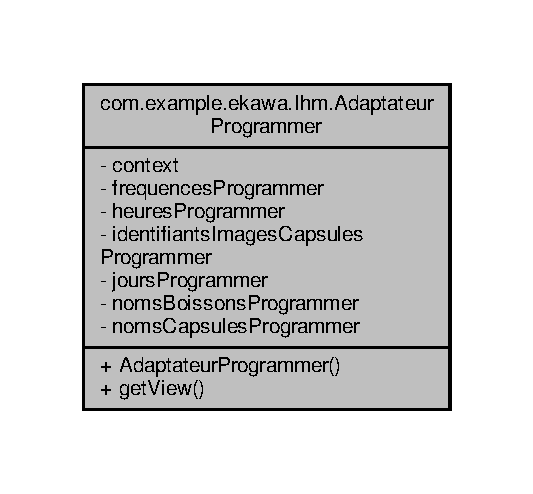
\includegraphics[width=256pt]{classcom_1_1example_1_1ekawa_1_1_ihm_1_1_adaptateur_programmer__coll__graph}
\end{center}
\end{figure}
\subsubsection*{Fonctions membres publiques}
\begin{DoxyCompactItemize}
\item 
\hyperlink{classcom_1_1example_1_1ekawa_1_1_ihm_1_1_adaptateur_programmer_a8a6bb79a26e790339065f37777890a34}{Adaptateur\+Programmer} (Activity \hyperlink{classcom_1_1example_1_1ekawa_1_1_ihm_1_1_adaptateur_programmer_aa2573f7d985ef662075730cb36a80f8a}{context}, Array\+List$<$ \hyperlink{classcom_1_1example_1_1ekawa_1_1_programmation}{Programmation} $>$ programmations)
\item 
View \hyperlink{classcom_1_1example_1_1ekawa_1_1_ihm_1_1_adaptateur_programmer_a948e7fa6ac9d148823e9f9dd3fba2f64}{get\+View} (int position, View item\+Converti, View\+Group parent)
\end{DoxyCompactItemize}
\subsubsection*{Attributs privés}
\begin{DoxyCompactItemize}
\item 
Activity \hyperlink{classcom_1_1example_1_1ekawa_1_1_ihm_1_1_adaptateur_programmer_aa2573f7d985ef662075730cb36a80f8a}{context}
\item 
Array\+List$<$ String $>$ \hyperlink{classcom_1_1example_1_1ekawa_1_1_ihm_1_1_adaptateur_programmer_a877b83e1a28ac8f704052df39aad695e}{frequences\+Programmer}
\item 
Array\+List$<$ String $>$ \hyperlink{classcom_1_1example_1_1ekawa_1_1_ihm_1_1_adaptateur_programmer_a114578f4eb2a34e7d3a258635c2ad9f1}{heures\+Programmer}
\item 
Array\+List$<$ Integer $>$ \hyperlink{classcom_1_1example_1_1ekawa_1_1_ihm_1_1_adaptateur_programmer_a468b21b654bd1c5cc663e1abf34c62ba}{identifiants\+Images\+Capsules\+Programmer}
\item 
Array\+List$<$ String $>$ \hyperlink{classcom_1_1example_1_1ekawa_1_1_ihm_1_1_adaptateur_programmer_a935bc1f05da276a491141ff78b66dad6}{jours\+Programmer}
\item 
Array\+List$<$ String $>$ \hyperlink{classcom_1_1example_1_1ekawa_1_1_ihm_1_1_adaptateur_programmer_a6cf686ef8f8c82dee10e609c7544a8e6}{noms\+Boissons\+Programmer}
\item 
Array\+List$<$ String $>$ \hyperlink{classcom_1_1example_1_1ekawa_1_1_ihm_1_1_adaptateur_programmer_ae079ecc919f92004afb238e01bb53928}{noms\+Capsules\+Programmer}
\end{DoxyCompactItemize}


\subsubsection{Description détaillée}


Définition à la ligne \hyperlink{_ihm_8java_source_l00180}{180} du fichier \hyperlink{_ihm_8java_source}{Ihm.\+java}.



\subsubsection{Documentation des constructeurs et destructeur}
\mbox{\Hypertarget{classcom_1_1example_1_1ekawa_1_1_ihm_1_1_adaptateur_programmer_a8a6bb79a26e790339065f37777890a34}\label{classcom_1_1example_1_1ekawa_1_1_ihm_1_1_adaptateur_programmer_a8a6bb79a26e790339065f37777890a34}} 
\index{com\+::example\+::ekawa\+::\+Ihm\+::\+Adaptateur\+Programmer@{com\+::example\+::ekawa\+::\+Ihm\+::\+Adaptateur\+Programmer}!Adaptateur\+Programmer@{Adaptateur\+Programmer}}
\index{Adaptateur\+Programmer@{Adaptateur\+Programmer}!com\+::example\+::ekawa\+::\+Ihm\+::\+Adaptateur\+Programmer@{com\+::example\+::ekawa\+::\+Ihm\+::\+Adaptateur\+Programmer}}
\paragraph{\texorpdfstring{Adaptateur\+Programmer()}{AdaptateurProgrammer()}}
{\footnotesize\ttfamily com.\+example.\+ekawa.\+Ihm.\+Adaptateur\+Programmer.\+Adaptateur\+Programmer (\begin{DoxyParamCaption}\item[{Activity}]{context,  }\item[{Array\+List$<$ \hyperlink{classcom_1_1example_1_1ekawa_1_1_programmation}{Programmation} $>$}]{programmations }\end{DoxyParamCaption})}



Définition à la ligne \hyperlink{_ihm_8java_source_l00190}{190} du fichier \hyperlink{_ihm_8java_source}{Ihm.\+java}.



Références \hyperlink{_ihm_8java_source_l00152}{com.\+example.\+ekawa.\+Ihm.\+Adaptateur\+Selection.\+context}, \hyperlink{_programmation_8java_source_l00067}{com.\+example.\+ekawa.\+Programmation.\+Frequences.\+F\+R\+E\+Q\+U\+E\+N\+C\+ES}, et \hyperlink{_programmation_8java_source_l00047}{com.\+example.\+ekawa.\+Programmation.\+Jours.\+J\+O\+U\+RS}.


\begin{DoxyCode}
00191         \{
00192             super(\hyperlink{classcom_1_1example_1_1ekawa_1_1_ihm_1_1_adaptateur_programmer_aa2573f7d985ef662075730cb36a80f8a}{context}, R.layout.item\_selection, programmations);
00193             this.\hyperlink{classcom_1_1example_1_1ekawa_1_1_ihm_1_1_adaptateur_programmer_aa2573f7d985ef662075730cb36a80f8a}{context} = \hyperlink{classcom_1_1example_1_1ekawa_1_1_ihm_1_1_adaptateur_programmer_aa2573f7d985ef662075730cb36a80f8a}{context};
00194             \hyperlink{classcom_1_1example_1_1ekawa_1_1_ihm_1_1_adaptateur_programmer_ae079ecc919f92004afb238e01bb53928}{nomsCapsulesProgrammer} = \textcolor{keyword}{new} ArrayList<String>();
00195             \hyperlink{classcom_1_1example_1_1ekawa_1_1_ihm_1_1_adaptateur_programmer_a6cf686ef8f8c82dee10e609c7544a8e6}{nomsBoissonsProgrammer} = \textcolor{keyword}{new} ArrayList<String>();
00196             \hyperlink{classcom_1_1example_1_1ekawa_1_1_ihm_1_1_adaptateur_programmer_a468b21b654bd1c5cc663e1abf34c62ba}{identifiantsImagesCapsulesProgrammer} = \textcolor{keyword}{new} 
      ArrayList<Integer>();
00197             \hyperlink{classcom_1_1example_1_1ekawa_1_1_ihm_1_1_adaptateur_programmer_a935bc1f05da276a491141ff78b66dad6}{joursProgrammer} = \textcolor{keyword}{new} ArrayList<String>();
00198             \hyperlink{classcom_1_1example_1_1ekawa_1_1_ihm_1_1_adaptateur_programmer_a114578f4eb2a34e7d3a258635c2ad9f1}{heuresProgrammer} = \textcolor{keyword}{new} ArrayList<String>();
00199             \hyperlink{classcom_1_1example_1_1ekawa_1_1_ihm_1_1_adaptateur_programmer_a877b83e1a28ac8f704052df39aad695e}{frequencesProgrammer} = \textcolor{keyword}{new} ArrayList<String>();
00200             \textcolor{keywordflow}{for} (Programmation programmation : programmations)
00201             \{
00202                 this.\hyperlink{classcom_1_1example_1_1ekawa_1_1_ihm_1_1_adaptateur_programmer_ae079ecc919f92004afb238e01bb53928}{nomsCapsulesProgrammer}.add(
      \hyperlink{classcom_1_1example_1_1ekawa_1_1_ihm_a9d61b7bfd998d449bb405dcf5e6e4e89}{nomsCapsules}[programmation.obtenirCapsule()]);
00203                 this.nomsBoissonsProgrammer.add(\hyperlink{classcom_1_1example_1_1ekawa_1_1_ihm_abafa700d1d1f943bd3e9678f698ed33a}{nomsBoisson}[programmation.obtenirBoisson()]);
00204                 this.identifiantsImagesCapsulesProgrammer.add(
      \hyperlink{classcom_1_1example_1_1ekawa_1_1_ihm_af35b42764d9f7b10c8bc0e210c3ba76d}{identifiantsImagesCapsules}[programmation.obtenirCapsule()]);
00205                 this.joursProgrammer.add(Programmation.Jours.JOURS[programmation.obtenirJour()]);
00206                 this.heuresProgrammer.add(programmation.obtenirHeure());
00207                 this.frequencesProgrammer.add(Programmation.Frequences.FREQUENCES[programmation.
      obtenirFrequence()]);
00208             \}
00209         \}
\end{DoxyCode}


\subsubsection{Documentation des fonctions membres}
\mbox{\Hypertarget{classcom_1_1example_1_1ekawa_1_1_ihm_1_1_adaptateur_programmer_a948e7fa6ac9d148823e9f9dd3fba2f64}\label{classcom_1_1example_1_1ekawa_1_1_ihm_1_1_adaptateur_programmer_a948e7fa6ac9d148823e9f9dd3fba2f64}} 
\index{com\+::example\+::ekawa\+::\+Ihm\+::\+Adaptateur\+Programmer@{com\+::example\+::ekawa\+::\+Ihm\+::\+Adaptateur\+Programmer}!get\+View@{get\+View}}
\index{get\+View@{get\+View}!com\+::example\+::ekawa\+::\+Ihm\+::\+Adaptateur\+Programmer@{com\+::example\+::ekawa\+::\+Ihm\+::\+Adaptateur\+Programmer}}
\paragraph{\texorpdfstring{get\+View()}{getView()}}
{\footnotesize\ttfamily View com.\+example.\+ekawa.\+Ihm.\+Adaptateur\+Programmer.\+get\+View (\begin{DoxyParamCaption}\item[{int}]{position,  }\item[{View}]{item\+Converti,  }\item[{View\+Group}]{parent }\end{DoxyParamCaption})}



Définition à la ligne \hyperlink{_ihm_8java_source_l00212}{212} du fichier \hyperlink{_ihm_8java_source}{Ihm.\+java}.


\begin{DoxyCode}
00213         \{
00214             View item = itemConverti;
00215             LayoutInflater inflater = \hyperlink{classcom_1_1example_1_1ekawa_1_1_ihm_1_1_adaptateur_programmer_aa2573f7d985ef662075730cb36a80f8a}{context}.getLayoutInflater();
00216             \textcolor{keywordflow}{if} (itemConverti == null)
00217                 item = inflater.inflate(R.layout.item\_programmer, null, \textcolor{keyword}{true});
00218             ImageView imageItem = (ImageView) item.findViewById(R.id.item\_image\_programmer);
00219             TextView texteCapsuleItem = (TextView) item.findViewById(R.id.item\_capsule);
00220             TextView texteBoissonItem = (TextView) item.findViewById(R.id.item\_boisson);
00221             TextView texteJourHeureItem = (TextView) item.findViewById(R.id.item\_jour\_heure);
00222             TextView texteFrequenceItem = (TextView) item.findViewById(R.id.item\_frequence);
00223 
00224             \textcolor{keywordflow}{if}(position == 0)
00225             \{
00226                 imageItem.setImageResource(R.drawable.ic\_plus);
00227                 texteCapsuleItem.setText(\textcolor{stringliteral}{""});
00228                 texteBoissonItem.setText(\textcolor{stringliteral}{""});
00229                 texteJourHeureItem.setText(\textcolor{stringliteral}{""});
00230                 texteFrequenceItem.setText(\textcolor{stringliteral}{""});
00231             \}
00232             \textcolor{keywordflow}{else}
00233             \{
00234                 imageItem.setImageResource(\hyperlink{classcom_1_1example_1_1ekawa_1_1_ihm_1_1_adaptateur_programmer_a468b21b654bd1c5cc663e1abf34c62ba}{identifiantsImagesCapsulesProgrammer}
      .get(position));
00235                 texteCapsuleItem.setText(\hyperlink{classcom_1_1example_1_1ekawa_1_1_ihm_1_1_adaptateur_programmer_ae079ecc919f92004afb238e01bb53928}{nomsCapsulesProgrammer}.get(position));
00236                 texteBoissonItem.setText(\hyperlink{classcom_1_1example_1_1ekawa_1_1_ihm_1_1_adaptateur_programmer_a6cf686ef8f8c82dee10e609c7544a8e6}{nomsBoissonsProgrammer}.get(position));
00237                 texteJourHeureItem.setText(\hyperlink{classcom_1_1example_1_1ekawa_1_1_ihm_1_1_adaptateur_programmer_a935bc1f05da276a491141ff78b66dad6}{joursProgrammer}.get(position) + \textcolor{stringliteral}{" - "} + 
      \hyperlink{classcom_1_1example_1_1ekawa_1_1_ihm_1_1_adaptateur_programmer_a114578f4eb2a34e7d3a258635c2ad9f1}{heuresProgrammer}.get(position));
00238                 texteFrequenceItem.setText(\hyperlink{classcom_1_1example_1_1ekawa_1_1_ihm_1_1_adaptateur_programmer_a877b83e1a28ac8f704052df39aad695e}{frequencesProgrammer}.get(position));
00239             \}
00240             \textcolor{keywordflow}{return} item;
00241         \}
\end{DoxyCode}


\subsubsection{Documentation des données membres}
\mbox{\Hypertarget{classcom_1_1example_1_1ekawa_1_1_ihm_1_1_adaptateur_programmer_aa2573f7d985ef662075730cb36a80f8a}\label{classcom_1_1example_1_1ekawa_1_1_ihm_1_1_adaptateur_programmer_aa2573f7d985ef662075730cb36a80f8a}} 
\index{com\+::example\+::ekawa\+::\+Ihm\+::\+Adaptateur\+Programmer@{com\+::example\+::ekawa\+::\+Ihm\+::\+Adaptateur\+Programmer}!context@{context}}
\index{context@{context}!com\+::example\+::ekawa\+::\+Ihm\+::\+Adaptateur\+Programmer@{com\+::example\+::ekawa\+::\+Ihm\+::\+Adaptateur\+Programmer}}
\paragraph{\texorpdfstring{context}{context}}
{\footnotesize\ttfamily Activity com.\+example.\+ekawa.\+Ihm.\+Adaptateur\+Programmer.\+context\hspace{0.3cm}{\ttfamily [private]}}



Définition à la ligne \hyperlink{_ihm_8java_source_l00182}{182} du fichier \hyperlink{_ihm_8java_source}{Ihm.\+java}.

\mbox{\Hypertarget{classcom_1_1example_1_1ekawa_1_1_ihm_1_1_adaptateur_programmer_a877b83e1a28ac8f704052df39aad695e}\label{classcom_1_1example_1_1ekawa_1_1_ihm_1_1_adaptateur_programmer_a877b83e1a28ac8f704052df39aad695e}} 
\index{com\+::example\+::ekawa\+::\+Ihm\+::\+Adaptateur\+Programmer@{com\+::example\+::ekawa\+::\+Ihm\+::\+Adaptateur\+Programmer}!frequences\+Programmer@{frequences\+Programmer}}
\index{frequences\+Programmer@{frequences\+Programmer}!com\+::example\+::ekawa\+::\+Ihm\+::\+Adaptateur\+Programmer@{com\+::example\+::ekawa\+::\+Ihm\+::\+Adaptateur\+Programmer}}
\paragraph{\texorpdfstring{frequences\+Programmer}{frequencesProgrammer}}
{\footnotesize\ttfamily Array\+List$<$String$>$ com.\+example.\+ekawa.\+Ihm.\+Adaptateur\+Programmer.\+frequences\+Programmer\hspace{0.3cm}{\ttfamily [private]}}



Définition à la ligne \hyperlink{_ihm_8java_source_l00188}{188} du fichier \hyperlink{_ihm_8java_source}{Ihm.\+java}.

\mbox{\Hypertarget{classcom_1_1example_1_1ekawa_1_1_ihm_1_1_adaptateur_programmer_a114578f4eb2a34e7d3a258635c2ad9f1}\label{classcom_1_1example_1_1ekawa_1_1_ihm_1_1_adaptateur_programmer_a114578f4eb2a34e7d3a258635c2ad9f1}} 
\index{com\+::example\+::ekawa\+::\+Ihm\+::\+Adaptateur\+Programmer@{com\+::example\+::ekawa\+::\+Ihm\+::\+Adaptateur\+Programmer}!heures\+Programmer@{heures\+Programmer}}
\index{heures\+Programmer@{heures\+Programmer}!com\+::example\+::ekawa\+::\+Ihm\+::\+Adaptateur\+Programmer@{com\+::example\+::ekawa\+::\+Ihm\+::\+Adaptateur\+Programmer}}
\paragraph{\texorpdfstring{heures\+Programmer}{heuresProgrammer}}
{\footnotesize\ttfamily Array\+List$<$String$>$ com.\+example.\+ekawa.\+Ihm.\+Adaptateur\+Programmer.\+heures\+Programmer\hspace{0.3cm}{\ttfamily [private]}}



Définition à la ligne \hyperlink{_ihm_8java_source_l00187}{187} du fichier \hyperlink{_ihm_8java_source}{Ihm.\+java}.

\mbox{\Hypertarget{classcom_1_1example_1_1ekawa_1_1_ihm_1_1_adaptateur_programmer_a468b21b654bd1c5cc663e1abf34c62ba}\label{classcom_1_1example_1_1ekawa_1_1_ihm_1_1_adaptateur_programmer_a468b21b654bd1c5cc663e1abf34c62ba}} 
\index{com\+::example\+::ekawa\+::\+Ihm\+::\+Adaptateur\+Programmer@{com\+::example\+::ekawa\+::\+Ihm\+::\+Adaptateur\+Programmer}!identifiants\+Images\+Capsules\+Programmer@{identifiants\+Images\+Capsules\+Programmer}}
\index{identifiants\+Images\+Capsules\+Programmer@{identifiants\+Images\+Capsules\+Programmer}!com\+::example\+::ekawa\+::\+Ihm\+::\+Adaptateur\+Programmer@{com\+::example\+::ekawa\+::\+Ihm\+::\+Adaptateur\+Programmer}}
\paragraph{\texorpdfstring{identifiants\+Images\+Capsules\+Programmer}{identifiantsImagesCapsulesProgrammer}}
{\footnotesize\ttfamily Array\+List$<$Integer$>$ com.\+example.\+ekawa.\+Ihm.\+Adaptateur\+Programmer.\+identifiants\+Images\+Capsules\+Programmer\hspace{0.3cm}{\ttfamily [private]}}



Définition à la ligne \hyperlink{_ihm_8java_source_l00185}{185} du fichier \hyperlink{_ihm_8java_source}{Ihm.\+java}.

\mbox{\Hypertarget{classcom_1_1example_1_1ekawa_1_1_ihm_1_1_adaptateur_programmer_a935bc1f05da276a491141ff78b66dad6}\label{classcom_1_1example_1_1ekawa_1_1_ihm_1_1_adaptateur_programmer_a935bc1f05da276a491141ff78b66dad6}} 
\index{com\+::example\+::ekawa\+::\+Ihm\+::\+Adaptateur\+Programmer@{com\+::example\+::ekawa\+::\+Ihm\+::\+Adaptateur\+Programmer}!jours\+Programmer@{jours\+Programmer}}
\index{jours\+Programmer@{jours\+Programmer}!com\+::example\+::ekawa\+::\+Ihm\+::\+Adaptateur\+Programmer@{com\+::example\+::ekawa\+::\+Ihm\+::\+Adaptateur\+Programmer}}
\paragraph{\texorpdfstring{jours\+Programmer}{joursProgrammer}}
{\footnotesize\ttfamily Array\+List$<$String$>$ com.\+example.\+ekawa.\+Ihm.\+Adaptateur\+Programmer.\+jours\+Programmer\hspace{0.3cm}{\ttfamily [private]}}



Définition à la ligne \hyperlink{_ihm_8java_source_l00186}{186} du fichier \hyperlink{_ihm_8java_source}{Ihm.\+java}.

\mbox{\Hypertarget{classcom_1_1example_1_1ekawa_1_1_ihm_1_1_adaptateur_programmer_a6cf686ef8f8c82dee10e609c7544a8e6}\label{classcom_1_1example_1_1ekawa_1_1_ihm_1_1_adaptateur_programmer_a6cf686ef8f8c82dee10e609c7544a8e6}} 
\index{com\+::example\+::ekawa\+::\+Ihm\+::\+Adaptateur\+Programmer@{com\+::example\+::ekawa\+::\+Ihm\+::\+Adaptateur\+Programmer}!noms\+Boissons\+Programmer@{noms\+Boissons\+Programmer}}
\index{noms\+Boissons\+Programmer@{noms\+Boissons\+Programmer}!com\+::example\+::ekawa\+::\+Ihm\+::\+Adaptateur\+Programmer@{com\+::example\+::ekawa\+::\+Ihm\+::\+Adaptateur\+Programmer}}
\paragraph{\texorpdfstring{noms\+Boissons\+Programmer}{nomsBoissonsProgrammer}}
{\footnotesize\ttfamily Array\+List$<$String$>$ com.\+example.\+ekawa.\+Ihm.\+Adaptateur\+Programmer.\+noms\+Boissons\+Programmer\hspace{0.3cm}{\ttfamily [private]}}



Définition à la ligne \hyperlink{_ihm_8java_source_l00184}{184} du fichier \hyperlink{_ihm_8java_source}{Ihm.\+java}.

\mbox{\Hypertarget{classcom_1_1example_1_1ekawa_1_1_ihm_1_1_adaptateur_programmer_ae079ecc919f92004afb238e01bb53928}\label{classcom_1_1example_1_1ekawa_1_1_ihm_1_1_adaptateur_programmer_ae079ecc919f92004afb238e01bb53928}} 
\index{com\+::example\+::ekawa\+::\+Ihm\+::\+Adaptateur\+Programmer@{com\+::example\+::ekawa\+::\+Ihm\+::\+Adaptateur\+Programmer}!noms\+Capsules\+Programmer@{noms\+Capsules\+Programmer}}
\index{noms\+Capsules\+Programmer@{noms\+Capsules\+Programmer}!com\+::example\+::ekawa\+::\+Ihm\+::\+Adaptateur\+Programmer@{com\+::example\+::ekawa\+::\+Ihm\+::\+Adaptateur\+Programmer}}
\paragraph{\texorpdfstring{noms\+Capsules\+Programmer}{nomsCapsulesProgrammer}}
{\footnotesize\ttfamily Array\+List$<$String$>$ com.\+example.\+ekawa.\+Ihm.\+Adaptateur\+Programmer.\+noms\+Capsules\+Programmer\hspace{0.3cm}{\ttfamily [private]}}



Définition à la ligne \hyperlink{_ihm_8java_source_l00183}{183} du fichier \hyperlink{_ihm_8java_source}{Ihm.\+java}.



La documentation de cette classe a été générée à partir du fichier suivant \+:\begin{DoxyCompactItemize}
\item 
\hyperlink{_ihm_8java}{Ihm.\+java}\end{DoxyCompactItemize}

\hypertarget{classcom_1_1example_1_1ekawa_1_1_ihm_1_1_adaptateur_selection}{}\subsection{Référence de la classe com.\+example.\+ekawa.\+Ihm.\+Adaptateur\+Selection}
\label{classcom_1_1example_1_1ekawa_1_1_ihm_1_1_adaptateur_selection}\index{com.\+example.\+ekawa.\+Ihm.\+Adaptateur\+Selection@{com.\+example.\+ekawa.\+Ihm.\+Adaptateur\+Selection}}


Graphe de collaboration de com.\+example.\+ekawa.\+Ihm.\+Adaptateur\+Selection\+:\nopagebreak
\begin{figure}[H]
\begin{center}
\leavevmode
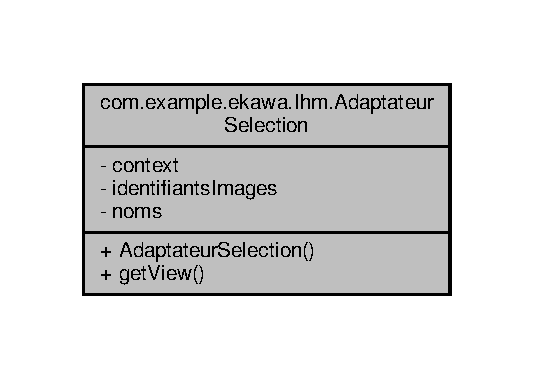
\includegraphics[width=256pt]{classcom_1_1example_1_1ekawa_1_1_ihm_1_1_adaptateur_selection__coll__graph}
\end{center}
\end{figure}
\subsubsection*{Fonctions membres publiques}
\begin{DoxyCompactItemize}
\item 
\hyperlink{classcom_1_1example_1_1ekawa_1_1_ihm_1_1_adaptateur_selection_a41746ec1a290651b4cacb0894a32307b}{Adaptateur\+Selection} (Activity \hyperlink{classcom_1_1example_1_1ekawa_1_1_ihm_1_1_adaptateur_selection_a9605d2f9384114fcb57da610a7071676}{context}, String\mbox{[}$\,$\mbox{]} \hyperlink{classcom_1_1example_1_1ekawa_1_1_ihm_1_1_adaptateur_selection_a5d71a6dd60ad53aa95ae59bb094b4002}{noms}, Integer\mbox{[}$\,$\mbox{]} identidiants\+Images)
\item 
View \hyperlink{classcom_1_1example_1_1ekawa_1_1_ihm_1_1_adaptateur_selection_a9c763267cefd3c67f449b8a797cdf916}{get\+View} (int position, View item\+Converti, View\+Group parent)
\end{DoxyCompactItemize}
\subsubsection*{Attributs privés}
\begin{DoxyCompactItemize}
\item 
Activity \hyperlink{classcom_1_1example_1_1ekawa_1_1_ihm_1_1_adaptateur_selection_a9605d2f9384114fcb57da610a7071676}{context}
\item 
Integer \mbox{[}$\,$\mbox{]} \hyperlink{classcom_1_1example_1_1ekawa_1_1_ihm_1_1_adaptateur_selection_ac242f0e242c82c556fb9bba16a5207d1}{identifiants\+Images}
\item 
String \mbox{[}$\,$\mbox{]} \hyperlink{classcom_1_1example_1_1ekawa_1_1_ihm_1_1_adaptateur_selection_a5d71a6dd60ad53aa95ae59bb094b4002}{noms}
\end{DoxyCompactItemize}


\subsubsection{Description détaillée}


Définition à la ligne \hyperlink{_ihm_8java_source_l00150}{150} du fichier \hyperlink{_ihm_8java_source}{Ihm.\+java}.



\subsubsection{Documentation des constructeurs et destructeur}
\mbox{\Hypertarget{classcom_1_1example_1_1ekawa_1_1_ihm_1_1_adaptateur_selection_a41746ec1a290651b4cacb0894a32307b}\label{classcom_1_1example_1_1ekawa_1_1_ihm_1_1_adaptateur_selection_a41746ec1a290651b4cacb0894a32307b}} 
\index{com\+::example\+::ekawa\+::\+Ihm\+::\+Adaptateur\+Selection@{com\+::example\+::ekawa\+::\+Ihm\+::\+Adaptateur\+Selection}!Adaptateur\+Selection@{Adaptateur\+Selection}}
\index{Adaptateur\+Selection@{Adaptateur\+Selection}!com\+::example\+::ekawa\+::\+Ihm\+::\+Adaptateur\+Selection@{com\+::example\+::ekawa\+::\+Ihm\+::\+Adaptateur\+Selection}}
\paragraph{\texorpdfstring{Adaptateur\+Selection()}{AdaptateurSelection()}}
{\footnotesize\ttfamily com.\+example.\+ekawa.\+Ihm.\+Adaptateur\+Selection.\+Adaptateur\+Selection (\begin{DoxyParamCaption}\item[{Activity}]{context,  }\item[{String \mbox{[}$\,$\mbox{]}}]{noms,  }\item[{Integer \mbox{[}$\,$\mbox{]}}]{identidiants\+Images }\end{DoxyParamCaption})}



Définition à la ligne \hyperlink{_ihm_8java_source_l00156}{156} du fichier \hyperlink{_ihm_8java_source}{Ihm.\+java}.



Références \hyperlink{_ihm_8java_source_l00152}{com.\+example.\+ekawa.\+Ihm.\+Adaptateur\+Selection.\+context}, et \hyperlink{_ihm_8java_source_l00153}{com.\+example.\+ekawa.\+Ihm.\+Adaptateur\+Selection.\+noms}.



Référencé par \hyperlink{_ihm_8java_source_l00727}{com.\+example.\+ekawa.\+Ihm.\+initialiser\+Fenetre\+Programmer()}, \hyperlink{_ihm_8java_source_l00637}{com.\+example.\+ekawa.\+Ihm.\+initialiser\+Page\+Informations()}, \hyperlink{_ihm_8java_source_l00470}{com.\+example.\+ekawa.\+Ihm.\+initialiser\+Selection\+Boisson()}, et \hyperlink{_ihm_8java_source_l00413}{com.\+example.\+ekawa.\+Ihm.\+initialiser\+Selection\+Capsule()}.


\begin{DoxyCode}
00157         \{
00158             super(\hyperlink{classcom_1_1example_1_1ekawa_1_1_ihm_1_1_adaptateur_selection_a9605d2f9384114fcb57da610a7071676}{context}, R.layout.item\_selection, \hyperlink{classcom_1_1example_1_1ekawa_1_1_ihm_1_1_adaptateur_selection_a5d71a6dd60ad53aa95ae59bb094b4002}{noms});
00159             this.\hyperlink{classcom_1_1example_1_1ekawa_1_1_ihm_1_1_adaptateur_selection_a9605d2f9384114fcb57da610a7071676}{context} = \hyperlink{classcom_1_1example_1_1ekawa_1_1_ihm_1_1_adaptateur_selection_a9605d2f9384114fcb57da610a7071676}{context};
00160             this.\hyperlink{classcom_1_1example_1_1ekawa_1_1_ihm_1_1_adaptateur_selection_a5d71a6dd60ad53aa95ae59bb094b4002}{noms} = \hyperlink{classcom_1_1example_1_1ekawa_1_1_ihm_1_1_adaptateur_selection_a5d71a6dd60ad53aa95ae59bb094b4002}{noms};
00161             this.\hyperlink{classcom_1_1example_1_1ekawa_1_1_ihm_1_1_adaptateur_selection_ac242f0e242c82c556fb9bba16a5207d1}{identifiantsImages} = identidiantsImages;
00162         \}
\end{DoxyCode}


\subsubsection{Documentation des fonctions membres}
\mbox{\Hypertarget{classcom_1_1example_1_1ekawa_1_1_ihm_1_1_adaptateur_selection_a9c763267cefd3c67f449b8a797cdf916}\label{classcom_1_1example_1_1ekawa_1_1_ihm_1_1_adaptateur_selection_a9c763267cefd3c67f449b8a797cdf916}} 
\index{com\+::example\+::ekawa\+::\+Ihm\+::\+Adaptateur\+Selection@{com\+::example\+::ekawa\+::\+Ihm\+::\+Adaptateur\+Selection}!get\+View@{get\+View}}
\index{get\+View@{get\+View}!com\+::example\+::ekawa\+::\+Ihm\+::\+Adaptateur\+Selection@{com\+::example\+::ekawa\+::\+Ihm\+::\+Adaptateur\+Selection}}
\paragraph{\texorpdfstring{get\+View()}{getView()}}
{\footnotesize\ttfamily View com.\+example.\+ekawa.\+Ihm.\+Adaptateur\+Selection.\+get\+View (\begin{DoxyParamCaption}\item[{int}]{position,  }\item[{View}]{item\+Converti,  }\item[{View\+Group}]{parent }\end{DoxyParamCaption})}



Définition à la ligne \hyperlink{_ihm_8java_source_l00165}{165} du fichier \hyperlink{_ihm_8java_source}{Ihm.\+java}.


\begin{DoxyCode}
00166         \{
00167             View item = itemConverti;
00168             LayoutInflater inflater = \hyperlink{classcom_1_1example_1_1ekawa_1_1_ihm_1_1_adaptateur_selection_a9605d2f9384114fcb57da610a7071676}{context}.getLayoutInflater();
00169             \textcolor{keywordflow}{if} (itemConverti == null)
00170                 item = inflater.inflate(R.layout.item\_selection, null, \textcolor{keyword}{true});
00171             ImageView imageItem = (ImageView) item.findViewById(R.id.item\_image);
00172             TextView texteItem = (TextView) item.findViewById(R.id.item\_texte);
00173 
00174             imageItem.setImageResource(\hyperlink{classcom_1_1example_1_1ekawa_1_1_ihm_1_1_adaptateur_selection_ac242f0e242c82c556fb9bba16a5207d1}{identifiantsImages}[position]);
00175             texteItem.setText(String.valueOf(position) + \textcolor{stringliteral}{" - "} + \hyperlink{classcom_1_1example_1_1ekawa_1_1_ihm_1_1_adaptateur_selection_a5d71a6dd60ad53aa95ae59bb094b4002}{noms}[position]);
00176             \textcolor{keywordflow}{return} item;
00177         \}
\end{DoxyCode}


\subsubsection{Documentation des données membres}
\mbox{\Hypertarget{classcom_1_1example_1_1ekawa_1_1_ihm_1_1_adaptateur_selection_a9605d2f9384114fcb57da610a7071676}\label{classcom_1_1example_1_1ekawa_1_1_ihm_1_1_adaptateur_selection_a9605d2f9384114fcb57da610a7071676}} 
\index{com\+::example\+::ekawa\+::\+Ihm\+::\+Adaptateur\+Selection@{com\+::example\+::ekawa\+::\+Ihm\+::\+Adaptateur\+Selection}!context@{context}}
\index{context@{context}!com\+::example\+::ekawa\+::\+Ihm\+::\+Adaptateur\+Selection@{com\+::example\+::ekawa\+::\+Ihm\+::\+Adaptateur\+Selection}}
\paragraph{\texorpdfstring{context}{context}}
{\footnotesize\ttfamily Activity com.\+example.\+ekawa.\+Ihm.\+Adaptateur\+Selection.\+context\hspace{0.3cm}{\ttfamily [private]}}



Définition à la ligne \hyperlink{_ihm_8java_source_l00152}{152} du fichier \hyperlink{_ihm_8java_source}{Ihm.\+java}.



Référencé par \hyperlink{_ihm_8java_source_l00190}{com.\+example.\+ekawa.\+Ihm.\+Adaptateur\+Programmer.\+Adaptateur\+Programmer()}, et \hyperlink{_ihm_8java_source_l00156}{com.\+example.\+ekawa.\+Ihm.\+Adaptateur\+Selection.\+Adaptateur\+Selection()}.

\mbox{\Hypertarget{classcom_1_1example_1_1ekawa_1_1_ihm_1_1_adaptateur_selection_ac242f0e242c82c556fb9bba16a5207d1}\label{classcom_1_1example_1_1ekawa_1_1_ihm_1_1_adaptateur_selection_ac242f0e242c82c556fb9bba16a5207d1}} 
\index{com\+::example\+::ekawa\+::\+Ihm\+::\+Adaptateur\+Selection@{com\+::example\+::ekawa\+::\+Ihm\+::\+Adaptateur\+Selection}!identifiants\+Images@{identifiants\+Images}}
\index{identifiants\+Images@{identifiants\+Images}!com\+::example\+::ekawa\+::\+Ihm\+::\+Adaptateur\+Selection@{com\+::example\+::ekawa\+::\+Ihm\+::\+Adaptateur\+Selection}}
\paragraph{\texorpdfstring{identifiants\+Images}{identifiantsImages}}
{\footnotesize\ttfamily Integer \mbox{[}$\,$\mbox{]} com.\+example.\+ekawa.\+Ihm.\+Adaptateur\+Selection.\+identifiants\+Images\hspace{0.3cm}{\ttfamily [private]}}



Définition à la ligne \hyperlink{_ihm_8java_source_l00154}{154} du fichier \hyperlink{_ihm_8java_source}{Ihm.\+java}.

\mbox{\Hypertarget{classcom_1_1example_1_1ekawa_1_1_ihm_1_1_adaptateur_selection_a5d71a6dd60ad53aa95ae59bb094b4002}\label{classcom_1_1example_1_1ekawa_1_1_ihm_1_1_adaptateur_selection_a5d71a6dd60ad53aa95ae59bb094b4002}} 
\index{com\+::example\+::ekawa\+::\+Ihm\+::\+Adaptateur\+Selection@{com\+::example\+::ekawa\+::\+Ihm\+::\+Adaptateur\+Selection}!noms@{noms}}
\index{noms@{noms}!com\+::example\+::ekawa\+::\+Ihm\+::\+Adaptateur\+Selection@{com\+::example\+::ekawa\+::\+Ihm\+::\+Adaptateur\+Selection}}
\paragraph{\texorpdfstring{noms}{noms}}
{\footnotesize\ttfamily String \mbox{[}$\,$\mbox{]} com.\+example.\+ekawa.\+Ihm.\+Adaptateur\+Selection.\+noms\hspace{0.3cm}{\ttfamily [private]}}



Définition à la ligne \hyperlink{_ihm_8java_source_l00153}{153} du fichier \hyperlink{_ihm_8java_source}{Ihm.\+java}.



Référencé par \hyperlink{_ihm_8java_source_l00156}{com.\+example.\+ekawa.\+Ihm.\+Adaptateur\+Selection.\+Adaptateur\+Selection()}.



La documentation de cette classe a été générée à partir du fichier suivant \+:\begin{DoxyCompactItemize}
\item 
\hyperlink{_ihm_8java}{Ihm.\+java}\end{DoxyCompactItemize}

\hypertarget{classcom_1_1example_1_1ekawa_1_1_boisson}{}\subsection{Référence de la classe com.\+example.\+ekawa.\+Boisson}
\label{classcom_1_1example_1_1ekawa_1_1_boisson}\index{com.\+example.\+ekawa.\+Boisson@{com.\+example.\+ekawa.\+Boisson}}


Définit les caractéristiques des boissons d\textquotesingle{}E\+K\+A\+WA.  




Graphe de collaboration de com.\+example.\+ekawa.\+Boisson\+:\nopagebreak
\begin{figure}[H]
\begin{center}
\leavevmode
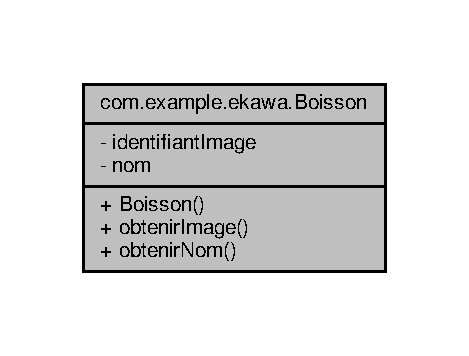
\includegraphics[width=225pt]{classcom_1_1example_1_1ekawa_1_1_boisson__coll__graph}
\end{center}
\end{figure}
\subsubsection*{Fonctions membres publiques}
\begin{DoxyCompactItemize}
\item 
\hyperlink{classcom_1_1example_1_1ekawa_1_1_boisson_a4dd8019f54eb6d1293a179ffe5e8b918}{Boisson} (String \hyperlink{classcom_1_1example_1_1ekawa_1_1_boisson_a9c932ca6665790c36acb6d4792a5a31a}{nom}, Integer \hyperlink{classcom_1_1example_1_1ekawa_1_1_boisson_ac73d259d39e459b00e5cfdf73a2aaf98}{identifiant\+Image})
\begin{DoxyCompactList}\small\item\em Constructeur de la classe \hyperlink{classcom_1_1example_1_1ekawa_1_1_boisson}{Boisson}. \end{DoxyCompactList}\item 
Integer \hyperlink{classcom_1_1example_1_1ekawa_1_1_boisson_a6edf9114dd70c1c16382136e57e6d345}{obtenir\+Image} ()
\begin{DoxyCompactList}\small\item\em Méthode qui permet d\textquotesingle{}obtenir l\textquotesingle{}identifiant de l\textquotesingle{}image de la boisson. \end{DoxyCompactList}\item 
String \hyperlink{classcom_1_1example_1_1ekawa_1_1_boisson_a410781851622f3c4b87a30d7381f9082}{obtenir\+Nom} ()
\begin{DoxyCompactList}\small\item\em Méthode qui permet d\textquotesingle{}obtenir le nom de la boisson. \end{DoxyCompactList}\end{DoxyCompactItemize}
\subsubsection*{Attributs privés}
\begin{DoxyCompactItemize}
\item 
Integer \hyperlink{classcom_1_1example_1_1ekawa_1_1_boisson_ac73d259d39e459b00e5cfdf73a2aaf98}{identifiant\+Image}
\item 
String \hyperlink{classcom_1_1example_1_1ekawa_1_1_boisson_a9c932ca6665790c36acb6d4792a5a31a}{nom}
\end{DoxyCompactItemize}


\subsubsection{Description détaillée}
Définit les caractéristiques des boissons d\textquotesingle{}E\+K\+A\+WA. 

Définition à la ligne \hyperlink{_boisson_8java_source_l00015}{15} du fichier \hyperlink{_boisson_8java_source}{Boisson.\+java}.



\subsubsection{Documentation des constructeurs et destructeur}
\mbox{\Hypertarget{classcom_1_1example_1_1ekawa_1_1_boisson_a4dd8019f54eb6d1293a179ffe5e8b918}\label{classcom_1_1example_1_1ekawa_1_1_boisson_a4dd8019f54eb6d1293a179ffe5e8b918}} 
\index{com\+::example\+::ekawa\+::\+Boisson@{com\+::example\+::ekawa\+::\+Boisson}!Boisson@{Boisson}}
\index{Boisson@{Boisson}!com\+::example\+::ekawa\+::\+Boisson@{com\+::example\+::ekawa\+::\+Boisson}}
\paragraph{\texorpdfstring{Boisson()}{Boisson()}}
{\footnotesize\ttfamily com.\+example.\+ekawa.\+Boisson.\+Boisson (\begin{DoxyParamCaption}\item[{String}]{nom,  }\item[{Integer}]{identifiant\+Image }\end{DoxyParamCaption})}



Constructeur de la classe \hyperlink{classcom_1_1example_1_1ekawa_1_1_boisson}{Boisson}. 


\begin{DoxyParams}{Paramètres}
{\em nom} & le nom de la boisson \\
\hline
{\em identifiant\+Image} & l\textquotesingle{}identifiant de l\textquotesingle{}image de la boisson \\
\hline
\end{DoxyParams}


Définition à la ligne \hyperlink{_boisson_8java_source_l00025}{25} du fichier \hyperlink{_boisson_8java_source}{Boisson.\+java}.



Références \hyperlink{_boisson_8java_source_l00018}{com.\+example.\+ekawa.\+Boisson.\+identifiant\+Image}, et \hyperlink{_boisson_8java_source_l00017}{com.\+example.\+ekawa.\+Boisson.\+nom}.


\begin{DoxyCode}
00026     \{
00027         this.\hyperlink{classcom_1_1example_1_1ekawa_1_1_boisson_a9c932ca6665790c36acb6d4792a5a31a}{nom} = \hyperlink{classcom_1_1example_1_1ekawa_1_1_boisson_a9c932ca6665790c36acb6d4792a5a31a}{nom};
00028         this.\hyperlink{classcom_1_1example_1_1ekawa_1_1_boisson_ac73d259d39e459b00e5cfdf73a2aaf98}{identifiantImage} = \hyperlink{classcom_1_1example_1_1ekawa_1_1_boisson_ac73d259d39e459b00e5cfdf73a2aaf98}{identifiantImage};
00029     \}
\end{DoxyCode}


\subsubsection{Documentation des fonctions membres}
\mbox{\Hypertarget{classcom_1_1example_1_1ekawa_1_1_boisson_a6edf9114dd70c1c16382136e57e6d345}\label{classcom_1_1example_1_1ekawa_1_1_boisson_a6edf9114dd70c1c16382136e57e6d345}} 
\index{com\+::example\+::ekawa\+::\+Boisson@{com\+::example\+::ekawa\+::\+Boisson}!obtenir\+Image@{obtenir\+Image}}
\index{obtenir\+Image@{obtenir\+Image}!com\+::example\+::ekawa\+::\+Boisson@{com\+::example\+::ekawa\+::\+Boisson}}
\paragraph{\texorpdfstring{obtenir\+Image()}{obtenirImage()}}
{\footnotesize\ttfamily Integer com.\+example.\+ekawa.\+Boisson.\+obtenir\+Image (\begin{DoxyParamCaption}{ }\end{DoxyParamCaption})}



Méthode qui permet d\textquotesingle{}obtenir l\textquotesingle{}identifiant de l\textquotesingle{}image de la boisson. 

\begin{DoxyReturn}{Renvoie}
Integer l\textquotesingle{}identifiant de l\textquotesingle{}image de la boisson 
\end{DoxyReturn}


Définition à la ligne \hyperlink{_boisson_8java_source_l00044}{44} du fichier \hyperlink{_boisson_8java_source}{Boisson.\+java}.



Références \hyperlink{_boisson_8java_source_l00018}{com.\+example.\+ekawa.\+Boisson.\+identifiant\+Image}.


\begin{DoxyCode}
00045     \{
00046         \textcolor{keywordflow}{return} this.\hyperlink{classcom_1_1example_1_1ekawa_1_1_boisson_ac73d259d39e459b00e5cfdf73a2aaf98}{identifiantImage};
00047     \}
\end{DoxyCode}
\mbox{\Hypertarget{classcom_1_1example_1_1ekawa_1_1_boisson_a410781851622f3c4b87a30d7381f9082}\label{classcom_1_1example_1_1ekawa_1_1_boisson_a410781851622f3c4b87a30d7381f9082}} 
\index{com\+::example\+::ekawa\+::\+Boisson@{com\+::example\+::ekawa\+::\+Boisson}!obtenir\+Nom@{obtenir\+Nom}}
\index{obtenir\+Nom@{obtenir\+Nom}!com\+::example\+::ekawa\+::\+Boisson@{com\+::example\+::ekawa\+::\+Boisson}}
\paragraph{\texorpdfstring{obtenir\+Nom()}{obtenirNom()}}
{\footnotesize\ttfamily String com.\+example.\+ekawa.\+Boisson.\+obtenir\+Nom (\begin{DoxyParamCaption}{ }\end{DoxyParamCaption})}



Méthode qui permet d\textquotesingle{}obtenir le nom de la boisson. 

\begin{DoxyReturn}{Renvoie}
String le nom de la boisson 
\end{DoxyReturn}


Définition à la ligne \hyperlink{_boisson_8java_source_l00035}{35} du fichier \hyperlink{_boisson_8java_source}{Boisson.\+java}.



Références \hyperlink{_boisson_8java_source_l00017}{com.\+example.\+ekawa.\+Boisson.\+nom}.


\begin{DoxyCode}
00036     \{
00037         \textcolor{keywordflow}{return} this.\hyperlink{classcom_1_1example_1_1ekawa_1_1_boisson_a9c932ca6665790c36acb6d4792a5a31a}{nom};
00038     \}
\end{DoxyCode}


\subsubsection{Documentation des données membres}
\mbox{\Hypertarget{classcom_1_1example_1_1ekawa_1_1_boisson_ac73d259d39e459b00e5cfdf73a2aaf98}\label{classcom_1_1example_1_1ekawa_1_1_boisson_ac73d259d39e459b00e5cfdf73a2aaf98}} 
\index{com\+::example\+::ekawa\+::\+Boisson@{com\+::example\+::ekawa\+::\+Boisson}!identifiant\+Image@{identifiant\+Image}}
\index{identifiant\+Image@{identifiant\+Image}!com\+::example\+::ekawa\+::\+Boisson@{com\+::example\+::ekawa\+::\+Boisson}}
\paragraph{\texorpdfstring{identifiant\+Image}{identifiantImage}}
{\footnotesize\ttfamily Integer com.\+example.\+ekawa.\+Boisson.\+identifiant\+Image\hspace{0.3cm}{\ttfamily [private]}}



Définition à la ligne \hyperlink{_boisson_8java_source_l00018}{18} du fichier \hyperlink{_boisson_8java_source}{Boisson.\+java}.



Référencé par \hyperlink{_boisson_8java_source_l00025}{com.\+example.\+ekawa.\+Boisson.\+Boisson()}, et \hyperlink{_boisson_8java_source_l00044}{com.\+example.\+ekawa.\+Boisson.\+obtenir\+Image()}.

\mbox{\Hypertarget{classcom_1_1example_1_1ekawa_1_1_boisson_a9c932ca6665790c36acb6d4792a5a31a}\label{classcom_1_1example_1_1ekawa_1_1_boisson_a9c932ca6665790c36acb6d4792a5a31a}} 
\index{com\+::example\+::ekawa\+::\+Boisson@{com\+::example\+::ekawa\+::\+Boisson}!nom@{nom}}
\index{nom@{nom}!com\+::example\+::ekawa\+::\+Boisson@{com\+::example\+::ekawa\+::\+Boisson}}
\paragraph{\texorpdfstring{nom}{nom}}
{\footnotesize\ttfamily String com.\+example.\+ekawa.\+Boisson.\+nom\hspace{0.3cm}{\ttfamily [private]}}



Définition à la ligne \hyperlink{_boisson_8java_source_l00017}{17} du fichier \hyperlink{_boisson_8java_source}{Boisson.\+java}.



Référencé par \hyperlink{_boisson_8java_source_l00025}{com.\+example.\+ekawa.\+Boisson.\+Boisson()}, et \hyperlink{_boisson_8java_source_l00035}{com.\+example.\+ekawa.\+Boisson.\+obtenir\+Nom()}.



La documentation de cette classe a été générée à partir du fichier suivant \+:\begin{DoxyCompactItemize}
\item 
\hyperlink{_boisson_8java}{Boisson.\+java}\end{DoxyCompactItemize}

\hypertarget{classcom_1_1example_1_1ekawa_1_1_cafetiere}{}\subsection{Référence de la classe com.\+example.\+ekawa.\+Cafetiere}
\label{classcom_1_1example_1_1ekawa_1_1_cafetiere}\index{com.\+example.\+ekawa.\+Cafetiere@{com.\+example.\+ekawa.\+Cafetiere}}


Déclaration de la classe principale de l\textquotesingle{}application.  




Graphe de collaboration de com.\+example.\+ekawa.\+Cafetiere\+:\nopagebreak
\begin{figure}[H]
\begin{center}
\leavevmode
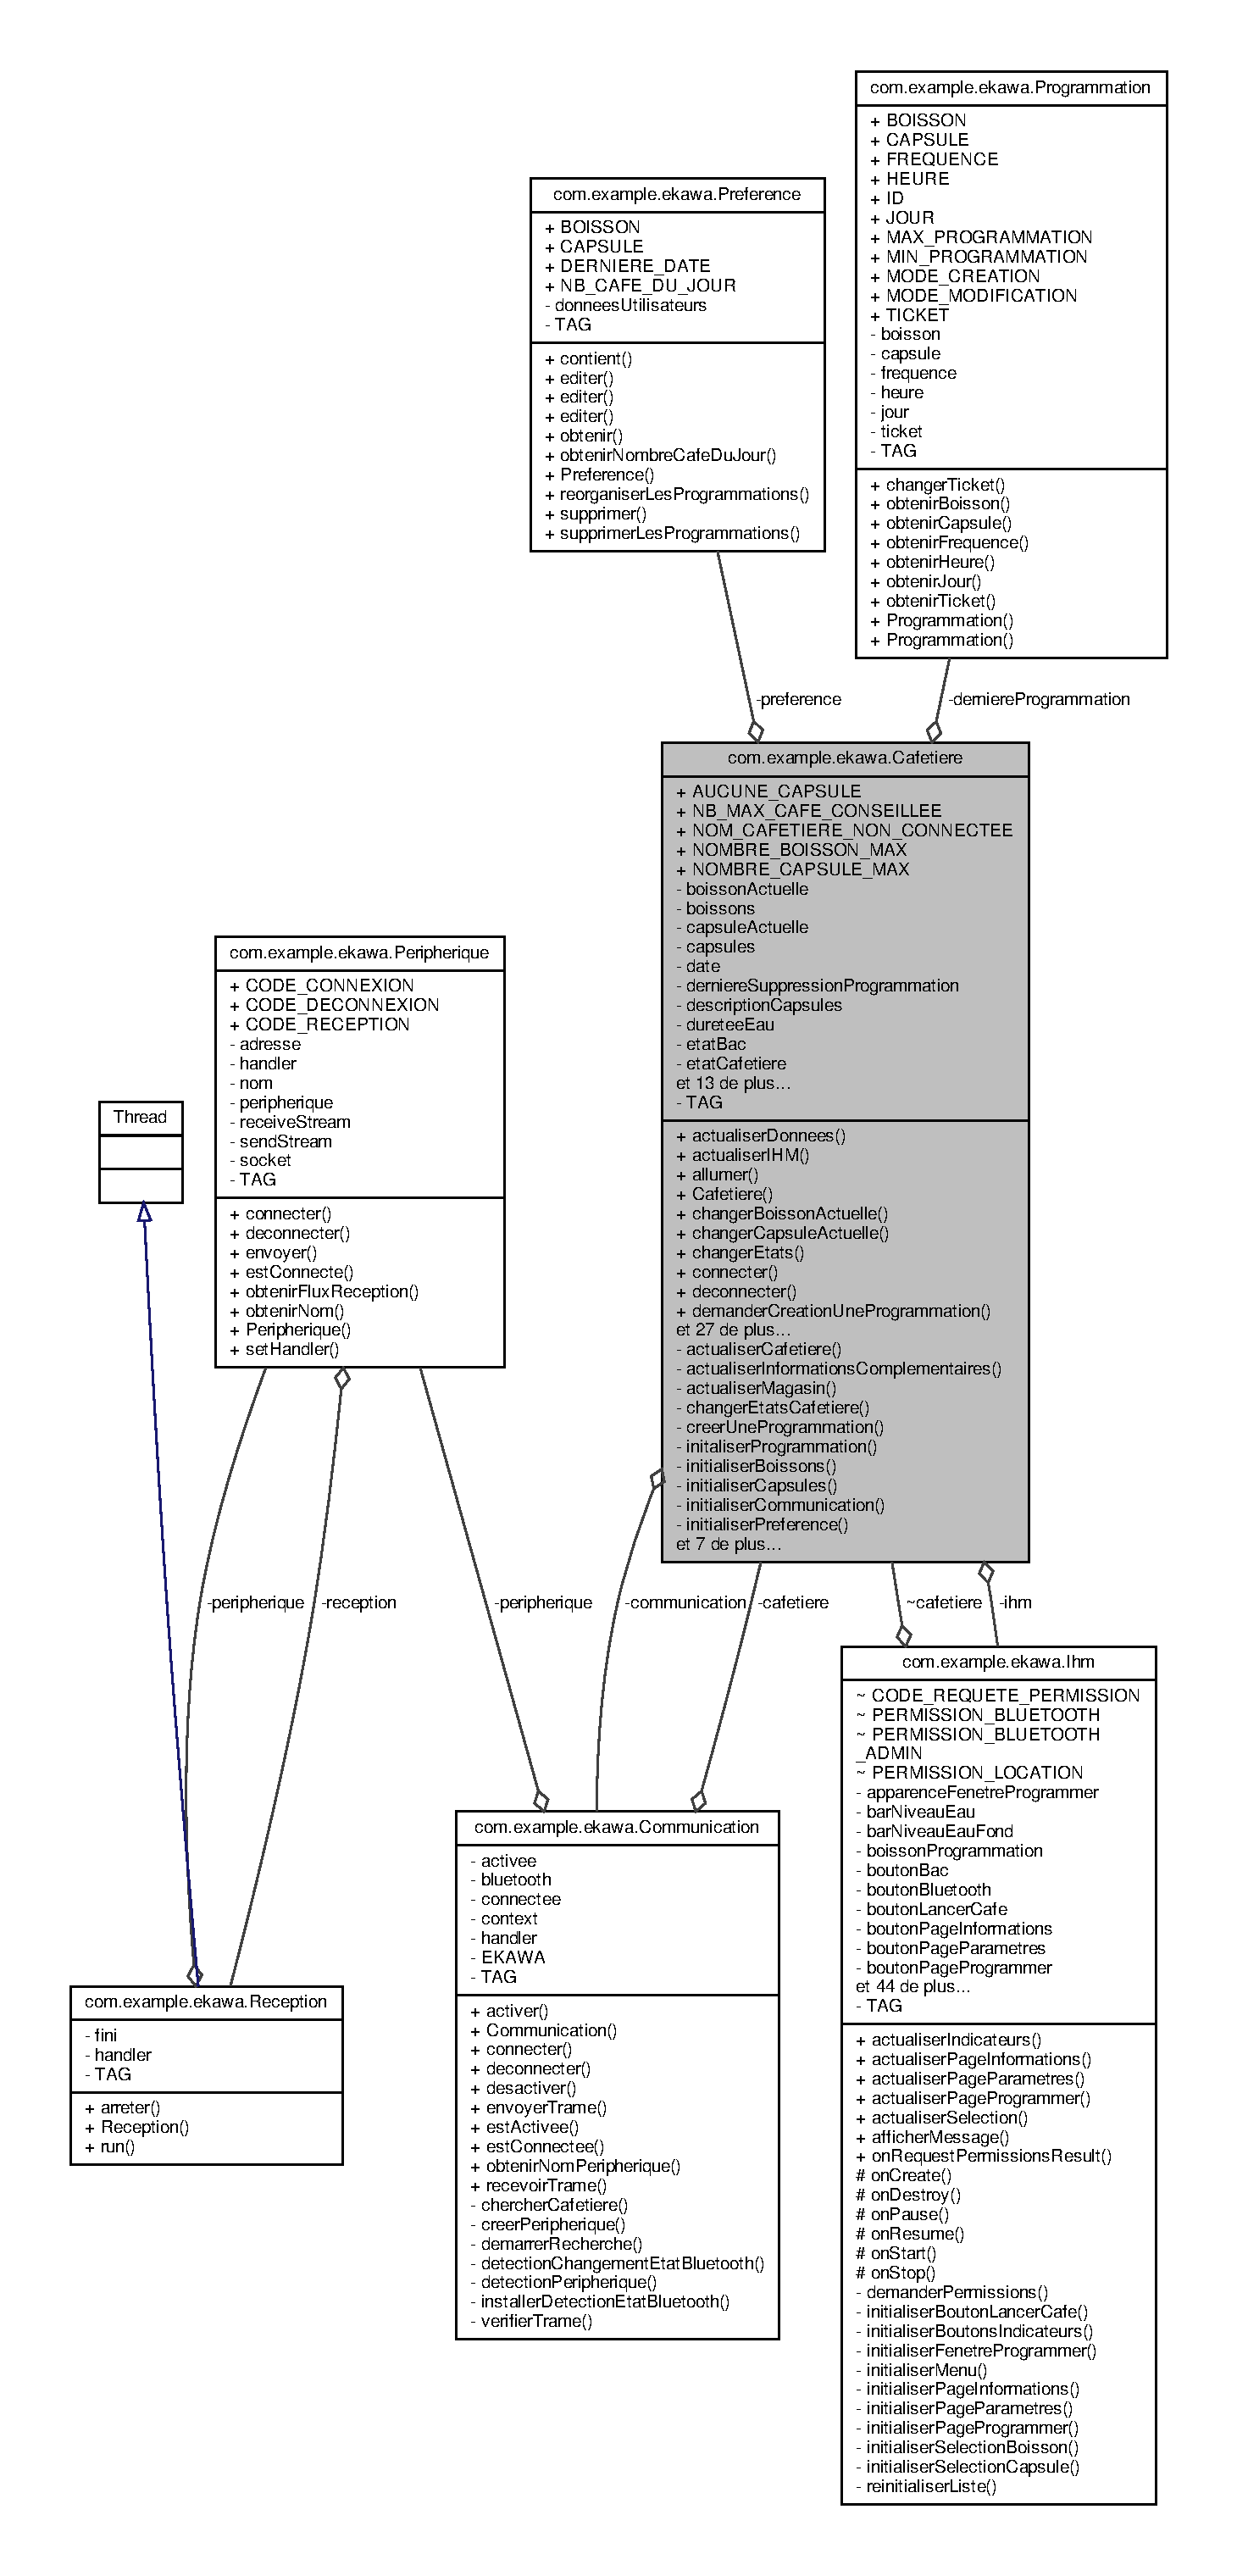
\includegraphics[height=550pt]{classcom_1_1example_1_1ekawa_1_1_cafetiere__coll__graph}
\end{center}
\end{figure}
\subsubsection*{Fonctions membres publiques}
\begin{DoxyCompactItemize}
\item 
void \hyperlink{classcom_1_1example_1_1ekawa_1_1_cafetiere_a1c6b2ea0e069cda876260e18ea8f6e84}{actualiser\+Donnees} ()
\begin{DoxyCompactList}\small\item\em Méthode qui permet d\textquotesingle{}envoyer les trames d\textquotesingle{}actualisations à la cafetière. \end{DoxyCompactList}\item 
void \hyperlink{classcom_1_1example_1_1ekawa_1_1_cafetiere_ad8c8b7d410315f55a216de809571fd87}{actualiser\+I\+HM} ()
\begin{DoxyCompactList}\small\item\em Méthode qui permet d\textquotesingle{}actualiser l\textquotesingle{}I\+HM. \end{DoxyCompactList}\item 
void \hyperlink{classcom_1_1example_1_1ekawa_1_1_cafetiere_afa405dc114a82fe74c06ff0971fa6cfc}{allumer} ()
\begin{DoxyCompactList}\small\item\em Méthode qui permet d\textquotesingle{}allumer le bluetooth. \end{DoxyCompactList}\item 
\hyperlink{classcom_1_1example_1_1ekawa_1_1_cafetiere_a8a8b762148526c605b13daeaf9d2e7cb}{Cafetiere} (\hyperlink{classcom_1_1example_1_1ekawa_1_1_ihm}{Ihm} \hyperlink{classcom_1_1example_1_1ekawa_1_1_cafetiere_a7db4a63088834eda5f6a3e951611bf82}{ihm})
\begin{DoxyCompactList}\small\item\em Constructeur de la classe Cafetière. \end{DoxyCompactList}\item 
void \hyperlink{classcom_1_1example_1_1ekawa_1_1_cafetiere_a50775b093a7f6d1b0fe8ad3662d80fc5}{changer\+Boisson\+Actuelle} (int boisson)
\begin{DoxyCompactList}\small\item\em Méthode qui modifie la boisson actuelle. \end{DoxyCompactList}\item 
void \hyperlink{classcom_1_1example_1_1ekawa_1_1_cafetiere_a686b4e821ea9164323753eb123576921}{changer\+Capsule\+Actuelle} (int capsule)
\begin{DoxyCompactList}\small\item\em Méthode qui modifie la capsule actuelle. \end{DoxyCompactList}\item 
void \hyperlink{classcom_1_1example_1_1ekawa_1_1_cafetiere_aba42bba06ffbf08735d7f548bcce9f42}{changer\+Etats} (String trame)
\begin{DoxyCompactList}\small\item\em Méthode qui permet d\textquotesingle{}actualiser les états de la cafetière, la tasse, le bac et le niveau d\textquotesingle{}eau + les présences des capsules. \end{DoxyCompactList}\item 
void \hyperlink{classcom_1_1example_1_1ekawa_1_1_cafetiere_a7ea38fe01cdeb8588fc34de028907a9c}{connecter} ()
\begin{DoxyCompactList}\small\item\em Méthode qui permet de connecter le bluetooth à la cafetière. \end{DoxyCompactList}\item 
void \hyperlink{classcom_1_1example_1_1ekawa_1_1_cafetiere_a8bf7e4352dafd60485555ee68edb9e52}{deconnecter} ()
\begin{DoxyCompactList}\small\item\em Méthode qui permet de deconnecter le bluetooth de la cafetière. \end{DoxyCompactList}\item 
void \hyperlink{classcom_1_1example_1_1ekawa_1_1_cafetiere_a2657310905f93ef4fba5b5f1dad81be9}{demander\+Creation\+Une\+Programmation} (int capsule, int boisson, int jour, String heure, int frequence)
\begin{DoxyCompactList}\small\item\em Méthode qui permet de demander la création d\textquotesingle{}une programmation. \end{DoxyCompactList}\item 
void \hyperlink{classcom_1_1example_1_1ekawa_1_1_cafetiere_a76eb3aa494815ac3b43371e21de21db3}{demander\+Preparation\+Cafe} ()
\begin{DoxyCompactList}\small\item\em Méthode qui permet de lancer la préparation d\textquotesingle{}un café \end{DoxyCompactList}\item 
void \hyperlink{classcom_1_1example_1_1ekawa_1_1_cafetiere_a0af9bf8f80c745c7919ea3efdc2183d0}{demander\+Suppression\+Une\+Programmation} (int position)
\begin{DoxyCompactList}\small\item\em Méthode qui permet de demander la suppression d\textquotesingle{}une programmation. \end{DoxyCompactList}\item 
void \hyperlink{classcom_1_1example_1_1ekawa_1_1_cafetiere_acca6b757d8fad0d0faf64f3266557ca2}{eteindre} ()
\begin{DoxyCompactList}\small\item\em Méthode qui permet d\textquotesingle{}eteindre le bluetooth. \end{DoxyCompactList}\item 
int \hyperlink{classcom_1_1example_1_1ekawa_1_1_cafetiere_aa7022512d5a36d2b911722ae6400379f}{informer\+Boisson\+Actuelle} ()
\begin{DoxyCompactList}\small\item\em Méthode qui renvoie la boisson actuelle. \end{DoxyCompactList}\item 
int \hyperlink{classcom_1_1example_1_1ekawa_1_1_cafetiere_a3251d1865f3a4113553e1743a971984d}{informer\+Capsule\+Actuelle} ()
\begin{DoxyCompactList}\small\item\em Méthode qui renvoie la capsule actuelle. \end{DoxyCompactList}\item 
boolean \hyperlink{classcom_1_1example_1_1ekawa_1_1_cafetiere_a97d9ca4701a961fe8865ecfa1d5bf64a}{informer\+Connexion\+Bluetooth} ()
\begin{DoxyCompactList}\small\item\em Méthode qui renvoie si le bluetooth est connecté ou non. \end{DoxyCompactList}\item 
int \hyperlink{classcom_1_1example_1_1ekawa_1_1_cafetiere_a078b7b5343bfbc06dec35dbd8fb292be}{informer\+Duretee\+Eau} ()
\begin{DoxyCompactList}\small\item\em Méthode qui renvoie la duretee de l\textquotesingle{}eau. \end{DoxyCompactList}\item 
boolean \hyperlink{classcom_1_1example_1_1ekawa_1_1_cafetiere_a1e5aad72cec77a755c8b70eb1be5e6e5}{informer\+Etat\+Bac} ()
\begin{DoxyCompactList}\small\item\em Méthode qui renvoie si le bac est plein ou non. \end{DoxyCompactList}\item 
boolean \hyperlink{classcom_1_1example_1_1ekawa_1_1_cafetiere_aeff88ad385713a7897074dcdb76077a5}{informer\+Etat\+Bluetooth} ()
\begin{DoxyCompactList}\small\item\em Méthode qui renvoie si le bluetooth est activé ou non. \end{DoxyCompactList}\item 
boolean \hyperlink{classcom_1_1example_1_1ekawa_1_1_cafetiere_a4253a092cf9c84f7b97021e628d5bfb4}{informer\+Etat\+Cafetiere} ()
\begin{DoxyCompactList}\small\item\em Méthode qui renvoie si la cafetière est utilisable ou non. \end{DoxyCompactList}\item 
boolean \hyperlink{classcom_1_1example_1_1ekawa_1_1_cafetiere_ae3c04cc0258cbe554eee5894655c379e}{informer\+Etat\+Tasse} ()
\begin{DoxyCompactList}\small\item\em Méthode qui renvoie si la tasse est bien placée ou non. \end{DoxyCompactList}\item 
int \hyperlink{classcom_1_1example_1_1ekawa_1_1_cafetiere_ab8113e922056276f8097744991ca76b6}{informer\+Niveau\+Eau} ()
\begin{DoxyCompactList}\small\item\em Méthode qui renvoie le niveau d\textquotesingle{}eau. \end{DoxyCompactList}\item 
int \hyperlink{classcom_1_1example_1_1ekawa_1_1_cafetiere_a6c708e64b24c32926eb787c3e7b8645a}{informer\+Nombre\+Bac\+Vide} ()
\begin{DoxyCompactList}\small\item\em Méthode qui renvoie le nombre de bac videe. \end{DoxyCompactList}\item 
int \hyperlink{classcom_1_1example_1_1ekawa_1_1_cafetiere_ac93a294ca5d2dcd4cc9c54bf5c41c3e4}{informer\+Nombre\+Cafe\+Du\+Jour} ()
\begin{DoxyCompactList}\small\item\em Méthode qui renvoie le nombre de cafe du jour. \end{DoxyCompactList}\item 
int \hyperlink{classcom_1_1example_1_1ekawa_1_1_cafetiere_a01de1ada0bfd9d75e9c873ca1bdb62df}{informer\+Nombre\+Cafe\+Total} ()
\begin{DoxyCompactList}\small\item\em Méthode qui renvoie le nombre de café total. \end{DoxyCompactList}\item 
int \hyperlink{classcom_1_1example_1_1ekawa_1_1_cafetiere_a456c870bf52bcd639abdc299e50ddd73}{informer\+Nombre\+Eau\+Remplie} ()
\begin{DoxyCompactList}\small\item\em Méthode qui renvoie le nombre d\textquotesingle{}eau remplie. \end{DoxyCompactList}\item 
String \hyperlink{classcom_1_1example_1_1ekawa_1_1_cafetiere_aa267545b22527a434e812f8c001d1e8a}{informer\+Nom\+Cafetiere} ()
\begin{DoxyCompactList}\small\item\em Méthode qui renvoie le nom de la cafetière connectée. \end{DoxyCompactList}\item 
boolean \hyperlink{classcom_1_1example_1_1ekawa_1_1_cafetiere_a35a291f849346b374f63324bc3ecd70b}{informer\+Presence\+Capsule} (int position)
\begin{DoxyCompactList}\small\item\em Méthode qui renvoie le niveau d\textquotesingle{}eau. \end{DoxyCompactList}\item 
int \hyperlink{classcom_1_1example_1_1ekawa_1_1_cafetiere_a1c04bcbd87ed47f8abf08e36e0629e13}{informer\+Qualitee\+Eau} ()
\begin{DoxyCompactList}\small\item\em Méthode qui renvoie la qualitee de l\textquotesingle{}eau. \end{DoxyCompactList}\item 
Array\+List$<$ \hyperlink{classcom_1_1example_1_1ekawa_1_1_boisson}{Boisson} $>$ \hyperlink{classcom_1_1example_1_1ekawa_1_1_cafetiere_a508a256d85a4e78c2b5c1a45899fcd99}{lister\+Boissons} ()
\begin{DoxyCompactList}\small\item\em Méthode qui renvoie la liste des boissons. \end{DoxyCompactList}\item 
Array\+List$<$ \hyperlink{classcom_1_1example_1_1ekawa_1_1_capsule}{Capsule} $>$ \hyperlink{classcom_1_1example_1_1ekawa_1_1_cafetiere_a86149d999dc196c3d97c855be0073e99}{lister\+Capsules} ()
\begin{DoxyCompactList}\small\item\em Méthode qui renvoie la liste des capsules. \end{DoxyCompactList}\item 
Array\+List$<$ \hyperlink{classcom_1_1example_1_1ekawa_1_1_programmation}{Programmation} $>$ \hyperlink{classcom_1_1example_1_1ekawa_1_1_cafetiere_af82120eee3f2f7dbb28f74e663bfe15a}{lister\+Programmations} ()
\begin{DoxyCompactList}\small\item\em Méthode qui renvoie tous les programmations. \end{DoxyCompactList}\item 
void \hyperlink{classcom_1_1example_1_1ekawa_1_1_cafetiere_ae15274dce04b0f875727b29e573fc83f}{modifier\+Une\+Programmation} (int position, int capsule, int boisson, int jour, String heure, int frequence)
\begin{DoxyCompactList}\small\item\em Méthode qui permet de modifier une programmation. \end{DoxyCompactList}\item 
Integer \hyperlink{classcom_1_1example_1_1ekawa_1_1_cafetiere_ac9ff316ec5e971d52f595dc4594e7b5b}{obtenir\+Description\+Capsule} (int position)
\begin{DoxyCompactList}\small\item\em Méthode qui renvoie la liste des boissons. \end{DoxyCompactList}\item 
\hyperlink{classcom_1_1example_1_1ekawa_1_1_programmation}{Programmation} \hyperlink{classcom_1_1example_1_1ekawa_1_1_cafetiere_aaaaa95b5ed36da9d14f5aa60116a66b8}{obtenir\+Programmation} (int position)
\begin{DoxyCompactList}\small\item\em Méthode qui renvoie une programmation. \end{DoxyCompactList}\item 
void \hyperlink{classcom_1_1example_1_1ekawa_1_1_cafetiere_a18e77fd60191cc0b2c7e247f72807096}{reinitialiser\+Informations} ()
\begin{DoxyCompactList}\small\item\em Méthode qui permet de reinitialiser les informations complémentaires. \end{DoxyCompactList}\item 
void \hyperlink{classcom_1_1example_1_1ekawa_1_1_cafetiere_a10a040b45cfaac52cd5c26049bf2d7b7}{remettre\+A\+Zero} ()
\begin{DoxyCompactList}\small\item\em Méthode qui permet de remettre les arguments à zéro. \end{DoxyCompactList}\end{DoxyCompactItemize}
\subsubsection*{Attributs publics statiques}
\begin{DoxyCompactItemize}
\item 
static final int \hyperlink{classcom_1_1example_1_1ekawa_1_1_cafetiere_a5a23a636fa5f2e5826458e700f453c16}{A\+U\+C\+U\+N\+E\+\_\+\+C\+A\+P\+S\+U\+LE} = -\/1
\begin{DoxyCompactList}\small\item\em L\textquotesingle{}indicateur qu\textquotesingle{}il n\textquotesingle{}y a aucune capsule sélectionnée. \end{DoxyCompactList}\item 
static final int \hyperlink{classcom_1_1example_1_1ekawa_1_1_cafetiere_a9e0cce07580820dfbc85696f1fb82aef}{N\+B\+\_\+\+M\+A\+X\+\_\+\+C\+A\+F\+E\+\_\+\+C\+O\+N\+S\+E\+I\+L\+L\+EE} = 4
\begin{DoxyCompactList}\small\item\em Le nombre de café conseillé par jour. \end{DoxyCompactList}\item 
static final String \hyperlink{classcom_1_1example_1_1ekawa_1_1_cafetiere_a5b10663105c7e3fd28dfd9d51b5e925f}{N\+O\+M\+\_\+\+C\+A\+F\+E\+T\+I\+E\+R\+E\+\_\+\+N\+O\+N\+\_\+\+C\+O\+N\+N\+E\+C\+T\+EE} = \char`\"{}Aucune\char`\"{}
\begin{DoxyCompactList}\small\item\em ??? \end{DoxyCompactList}\item 
static final Integer \hyperlink{classcom_1_1example_1_1ekawa_1_1_cafetiere_a2be5950bf3bb155b8396593d390b808b}{N\+O\+M\+B\+R\+E\+\_\+\+B\+O\+I\+S\+S\+O\+N\+\_\+\+M\+AX} = 2
\begin{DoxyCompactList}\small\item\em Le nombre maximal de types de boisson (court/long) \end{DoxyCompactList}\item 
static final Integer \hyperlink{classcom_1_1example_1_1ekawa_1_1_cafetiere_a183d96e89c056c4ac9c565bf8f24851e}{N\+O\+M\+B\+R\+E\+\_\+\+C\+A\+P\+S\+U\+L\+E\+\_\+\+M\+AX} = 8
\begin{DoxyCompactList}\small\item\em Le nombre maximal de capsules. \end{DoxyCompactList}\end{DoxyCompactItemize}
\subsubsection*{Fonctions membres privées}
\begin{DoxyCompactItemize}
\item 
void \hyperlink{classcom_1_1example_1_1ekawa_1_1_cafetiere_a6485aa7504eeb5c3c09accab52bb3ad1}{actualiser\+Cafetiere} (String trame)
\begin{DoxyCompactList}\small\item\em Méthode qui permet d\textquotesingle{}actualiser les états de la cafetière, la tasse, le bac et le niveau d\textquotesingle{}eau. \end{DoxyCompactList}\item 
void \hyperlink{classcom_1_1example_1_1ekawa_1_1_cafetiere_af968afecce6625f466b145a54e8b1d44}{actualiser\+Informations\+Complementaires} (String trame)
\begin{DoxyCompactList}\small\item\em Méthode qui permet d\textquotesingle{}actualiser et d\textquotesingle{}initialiser les informations complémentaires. \end{DoxyCompactList}\item 
void \hyperlink{classcom_1_1example_1_1ekawa_1_1_cafetiere_a406c04398043ee4abca9902828197d91}{actualiser\+Magasin} (String trame)
\begin{DoxyCompactList}\small\item\em Méthode qui permet d\textquotesingle{}actualiser les présences des capsules. \end{DoxyCompactList}\item 
void \hyperlink{classcom_1_1example_1_1ekawa_1_1_cafetiere_a6fa4b1560875b71d339a9f6c24c5336d}{changer\+Etats\+Cafetiere} (boolean \hyperlink{classcom_1_1example_1_1ekawa_1_1_cafetiere_ae170dd018d1e740b3bda080d1cc3d900}{etat\+Cafetiere}, boolean \hyperlink{classcom_1_1example_1_1ekawa_1_1_cafetiere_a93c5021591facf06397e760c11556904}{etat\+Tasse}, boolean \hyperlink{classcom_1_1example_1_1ekawa_1_1_cafetiere_a058f7a18cd9c0567d583b8bc6250d143}{etat\+Bac}, int \hyperlink{classcom_1_1example_1_1ekawa_1_1_cafetiere_aaf8e1a960f803c2de4defa414b5984a4}{niveau\+Eau})
\begin{DoxyCompactList}\small\item\em Méthode qui permet d\textquotesingle{}actualiser les états de la cafetière, la tasse, le bac et le niveau d\textquotesingle{}eau. \end{DoxyCompactList}\item 
void \hyperlink{classcom_1_1example_1_1ekawa_1_1_cafetiere_a8664d05f55227160182de50a7c31ccf3}{creer\+Une\+Programmation} (String trame)
\begin{DoxyCompactList}\small\item\em Méthode qui permet de créer une programmation. \end{DoxyCompactList}\item 
void \hyperlink{classcom_1_1example_1_1ekawa_1_1_cafetiere_aae065b86cdb3a8df2c904068aab7e9bf}{initaliser\+Programmation} ()
\item 
void \hyperlink{classcom_1_1example_1_1ekawa_1_1_cafetiere_ae9092a9540897e60c4cf7307073a75ab}{initialiser\+Boissons} ()
\begin{DoxyCompactList}\small\item\em Méthode qui permet d\textquotesingle{}initialiser la liste des boissons. \end{DoxyCompactList}\item 
void \hyperlink{classcom_1_1example_1_1ekawa_1_1_cafetiere_a75d0df422427eed8b12e7b46a6e11a35}{initialiser\+Capsules} ()
\begin{DoxyCompactList}\small\item\em Méthode qui permet d\textquotesingle{}initialiser la liste des capsules. \end{DoxyCompactList}\item 
void \hyperlink{classcom_1_1example_1_1ekawa_1_1_cafetiere_ad7c3e155b2ddf4dae05da8cd9c38518a}{initialiser\+Communication} ()
\begin{DoxyCompactList}\small\item\em Méthode qui permet d\textquotesingle{}initialiser la communication. \end{DoxyCompactList}\item 
void \hyperlink{classcom_1_1example_1_1ekawa_1_1_cafetiere_a20f3b74112d4e668a382882c4c8ccd07}{initialiser\+Preference} ()
\begin{DoxyCompactList}\small\item\em Méthode qui permet d\textquotesingle{}initialiser les préférences de l\textquotesingle{}utilisateur. \end{DoxyCompactList}\item 
void \hyperlink{classcom_1_1example_1_1ekawa_1_1_cafetiere_a406e5771edb1663ebb1fc571365b75ac}{initialiser\+Programmations} ()
\begin{DoxyCompactList}\small\item\em Méthode qui renvoie une programmation. \end{DoxyCompactList}\item 
void \hyperlink{classcom_1_1example_1_1ekawa_1_1_cafetiere_ac79907a8b3499bb9b2f50e31f8c904e8}{lancer\+Preparation\+Cafe} ()
\begin{DoxyCompactList}\small\item\em Méthode qui permet de lancer la préparation d\textquotesingle{}un café \end{DoxyCompactList}\item 
void \hyperlink{classcom_1_1example_1_1ekawa_1_1_cafetiere_a6d1bc4321c372f7639a3305cf74f10db}{supprimer\+Les\+Programmations} ()
\begin{DoxyCompactList}\small\item\em Méthode qui permet de suprimer toutes les programmations. \end{DoxyCompactList}\item 
void \hyperlink{classcom_1_1example_1_1ekawa_1_1_cafetiere_a40880363bf27354c1a7cb5df139fae53}{supprimer\+Une\+Programmation} ()
\begin{DoxyCompactList}\small\item\em Méthode qui permet de supprimer une programmation. \end{DoxyCompactList}\item 
void \hyperlink{classcom_1_1example_1_1ekawa_1_1_cafetiere_ac2f81a08528b9f7017bfe6183fde876f}{verifier\+Preparation\+Cafe} (String trame)
\begin{DoxyCompactList}\small\item\em Méthode qui permet de vérifier la trame de réponse d\textquotesingle{}une demande de préparation d\textquotesingle{}un café \end{DoxyCompactList}\item 
boolean \hyperlink{classcom_1_1example_1_1ekawa_1_1_cafetiere_ac3f2b337d1fd091faa312c2c6ec08bfc}{verifier\+Programmation} (String trame)
\begin{DoxyCompactList}\small\item\em Méthode qui permet de verifier si la programmation s\textquotesingle{}est bien lancer. \end{DoxyCompactList}\item 
void \hyperlink{classcom_1_1example_1_1ekawa_1_1_cafetiere_a316296ae1fad708259a403c60099caa1}{verifier\+Suppression\+Dune\+Programmation} (String trame)
\begin{DoxyCompactList}\small\item\em Méthode qui permet de vérifier la suppression d\textquotesingle{}une programmation. \end{DoxyCompactList}\end{DoxyCompactItemize}
\subsubsection*{Attributs privés}
\begin{DoxyCompactItemize}
\item 
int \hyperlink{classcom_1_1example_1_1ekawa_1_1_cafetiere_a73c5fa3b510655e1e3425140336b7f5b}{boisson\+Actuelle} = 0
\item 
Array\+List$<$ \hyperlink{classcom_1_1example_1_1ekawa_1_1_boisson}{Boisson} $>$ \hyperlink{classcom_1_1example_1_1ekawa_1_1_cafetiere_aad375efbc01f1db83572f4ae567189de}{boissons}
\item 
int \hyperlink{classcom_1_1example_1_1ekawa_1_1_cafetiere_ac8fa3d1ad76eccf431ee04b395a557a3}{capsule\+Actuelle} = \hyperlink{classcom_1_1example_1_1ekawa_1_1_cafetiere_a5a23a636fa5f2e5826458e700f453c16}{A\+U\+C\+U\+N\+E\+\_\+\+C\+A\+P\+S\+U\+LE}
\item 
Array\+List$<$ \hyperlink{classcom_1_1example_1_1ekawa_1_1_capsule}{Capsule} $>$ \hyperlink{classcom_1_1example_1_1ekawa_1_1_cafetiere_ae9590789503a6ae2094c86cf93299821}{capsules}
\item 
\hyperlink{classcom_1_1example_1_1ekawa_1_1_communication}{Communication} \hyperlink{classcom_1_1example_1_1ekawa_1_1_cafetiere_af9506a7805d000d2cb83444cdb8ea889}{communication} = null
\item 
String \hyperlink{classcom_1_1example_1_1ekawa_1_1_cafetiere_a61e4ab1e5ebdc60ffea39a344711e477}{date} = null
\item 
\hyperlink{classcom_1_1example_1_1ekawa_1_1_programmation}{Programmation} \hyperlink{classcom_1_1example_1_1ekawa_1_1_cafetiere_ae5fa359f1ddcbd80ce3651e2d7368ff8}{derniere\+Programmation}
\item 
int \hyperlink{classcom_1_1example_1_1ekawa_1_1_cafetiere_a79faede6506425563ec617affef48e09}{derniere\+Suppression\+Programmation}
\item 
Integer \mbox{[}$\,$\mbox{]} \hyperlink{classcom_1_1example_1_1ekawa_1_1_cafetiere_a054b6a7668e317cfa1da3d8600311e4e}{description\+Capsules}
\item 
int \hyperlink{classcom_1_1example_1_1ekawa_1_1_cafetiere_aafc365a43172fca9166fb2a9006c6ecf}{duretee\+Eau} = 0
\item 
boolean \hyperlink{classcom_1_1example_1_1ekawa_1_1_cafetiere_a058f7a18cd9c0567d583b8bc6250d143}{etat\+Bac} = false
\item 
boolean \hyperlink{classcom_1_1example_1_1ekawa_1_1_cafetiere_ae170dd018d1e740b3bda080d1cc3d900}{etat\+Cafetiere} = false
\item 
boolean \hyperlink{classcom_1_1example_1_1ekawa_1_1_cafetiere_a93c5021591facf06397e760c11556904}{etat\+Tasse} = false
\item 
Integer \mbox{[}$\,$\mbox{]} \hyperlink{classcom_1_1example_1_1ekawa_1_1_cafetiere_a10645115a166d3529e63aeb4ea16a869}{id\+Images\+Boissons} = \{ R.\+drawable.\+ic\+\_\+cafe\+\_\+court, R.\+drawable.\+ic\+\_\+cafe\+\_\+long \}
\item 
Integer \mbox{[}$\,$\mbox{]} \hyperlink{classcom_1_1example_1_1ekawa_1_1_cafetiere_a7558b3f423bd53d4198a7c143bd2d657}{id\+Images\+Capsules}
\item 
\hyperlink{classcom_1_1example_1_1ekawa_1_1_ihm}{Ihm} \hyperlink{classcom_1_1example_1_1ekawa_1_1_cafetiere_a7db4a63088834eda5f6a3e951611bf82}{ihm}
\item 
int \hyperlink{classcom_1_1example_1_1ekawa_1_1_cafetiere_aaf8e1a960f803c2de4defa414b5984a4}{niveau\+Eau} = 0
\item 
int \hyperlink{classcom_1_1example_1_1ekawa_1_1_cafetiere_a6491d6d04db5d6e7da868565b84f6d7f}{nombre\+Bac\+Vide} = 0
\item 
int \hyperlink{classcom_1_1example_1_1ekawa_1_1_cafetiere_a123b6fcb9a9c1decae40e026660e716b}{nombre\+Cafe\+Du\+Jour} = 0
\begin{DoxyCompactList}\small\item\em ??? \end{DoxyCompactList}\item 
int \hyperlink{classcom_1_1example_1_1ekawa_1_1_cafetiere_ac22f9da8ed59c7362871b8f22e501e23}{nombre\+Cafe\+Total} = 0
\begin{DoxyCompactList}\small\item\em ??? \end{DoxyCompactList}\item 
int \hyperlink{classcom_1_1example_1_1ekawa_1_1_cafetiere_a2332c2e33acff5084b4571663b48bd89}{nombre\+Eau\+Remplie} = 0
\item 
String \mbox{[}$\,$\mbox{]} \hyperlink{classcom_1_1example_1_1ekawa_1_1_cafetiere_a59db420b33a9f03aad97d6cad4f87c03}{noms\+Boissons} = \{ \char`\"{}Court\char`\"{}, \char`\"{}Long\char`\"{} \}
\item 
String \mbox{[}$\,$\mbox{]} \hyperlink{classcom_1_1example_1_1ekawa_1_1_cafetiere_a127a27c8f3b4c6c5dc4bfb639f654b3d}{noms\+Capusles}
\begin{DoxyCompactList}\small\item\em Exemples de noms de capsule. \end{DoxyCompactList}\item 
\hyperlink{classcom_1_1example_1_1ekawa_1_1_preference}{Preference} \hyperlink{classcom_1_1example_1_1ekawa_1_1_cafetiere_aee3f9b78df63bc8dd73bf564954d51ca}{preference} = null
\item 
boolean \mbox{[}$\,$\mbox{]} \hyperlink{classcom_1_1example_1_1ekawa_1_1_cafetiere_aebaaf300362a258e047ae31b7e56e622}{presences\+Capsules} = \{ true, true, true, true, true, true, true, true \}
\item 
Array\+List$<$ \hyperlink{classcom_1_1example_1_1ekawa_1_1_programmation}{Programmation} $>$ \hyperlink{classcom_1_1example_1_1ekawa_1_1_cafetiere_a987c8e1bcea506b65f4b05f955b3f699}{programmations}
\item 
int \hyperlink{classcom_1_1example_1_1ekawa_1_1_cafetiere_a27aba2ce49934d0bf7b2d2230b3003d7}{qualitee\+Eau} = 0
\end{DoxyCompactItemize}
\subsubsection*{Attributs privés statiques}
\begin{DoxyCompactItemize}
\item 
static final String \hyperlink{classcom_1_1example_1_1ekawa_1_1_cafetiere_aa0c1fd99a2508b06c462aea17034aa91}{T\+AG} = \char`\"{}Cafetiere\char`\"{}
\begin{DoxyCompactList}\small\item\em T\+AG pour les logs. \end{DoxyCompactList}\end{DoxyCompactItemize}


\subsubsection{Description détaillée}
Déclaration de la classe principale de l\textquotesingle{}application. 

Définition à la ligne \hyperlink{_cafetiere_8java_source_l00022}{22} du fichier \hyperlink{_cafetiere_8java_source}{Cafetiere.\+java}.



\subsubsection{Documentation des constructeurs et destructeur}
\mbox{\Hypertarget{classcom_1_1example_1_1ekawa_1_1_cafetiere_a8a8b762148526c605b13daeaf9d2e7cb}\label{classcom_1_1example_1_1ekawa_1_1_cafetiere_a8a8b762148526c605b13daeaf9d2e7cb}} 
\index{com\+::example\+::ekawa\+::\+Cafetiere@{com\+::example\+::ekawa\+::\+Cafetiere}!Cafetiere@{Cafetiere}}
\index{Cafetiere@{Cafetiere}!com\+::example\+::ekawa\+::\+Cafetiere@{com\+::example\+::ekawa\+::\+Cafetiere}}
\paragraph{\texorpdfstring{Cafetiere()}{Cafetiere()}}
{\footnotesize\ttfamily com.\+example.\+ekawa.\+Cafetiere.\+Cafetiere (\begin{DoxyParamCaption}\item[{\hyperlink{classcom_1_1example_1_1ekawa_1_1_ihm}{Ihm}}]{ihm }\end{DoxyParamCaption})}



Constructeur de la classe Cafetière. 


\begin{DoxyParams}{Paramètres}
{\em ihm} & l\textquotesingle{}ihm \\
\hline
\end{DoxyParams}


Définition à la ligne \hyperlink{_cafetiere_8java_source_l00108}{108} du fichier \hyperlink{_cafetiere_8java_source}{Cafetiere.\+java}.



Références \hyperlink{_cafetiere_8java_source_l00080}{com.\+example.\+ekawa.\+Cafetiere.\+ihm}, \hyperlink{_cafetiere_8java_source_l00143}{com.\+example.\+ekawa.\+Cafetiere.\+initaliser\+Programmation()}, \hyperlink{_cafetiere_8java_source_l00173}{com.\+example.\+ekawa.\+Cafetiere.\+initialiser\+Boissons()}, \hyperlink{_cafetiere_8java_source_l00162}{com.\+example.\+ekawa.\+Cafetiere.\+initialiser\+Capsules()}, \hyperlink{_cafetiere_8java_source_l00153}{com.\+example.\+ekawa.\+Cafetiere.\+initialiser\+Communication()}, et \hyperlink{_cafetiere_8java_source_l00122}{com.\+example.\+ekawa.\+Cafetiere.\+initialiser\+Preference()}.


\begin{DoxyCode}
00109     \{
00110         Log.d(\hyperlink{classcom_1_1example_1_1ekawa_1_1_cafetiere_aa0c1fd99a2508b06c462aea17034aa91}{TAG}, \textcolor{stringliteral}{"Cafetiere()"});
00111         this.\hyperlink{classcom_1_1example_1_1ekawa_1_1_cafetiere_a7db4a63088834eda5f6a3e951611bf82}{ihm} = \hyperlink{classcom_1_1example_1_1ekawa_1_1_cafetiere_a7db4a63088834eda5f6a3e951611bf82}{ihm};
00112         \hyperlink{classcom_1_1example_1_1ekawa_1_1_cafetiere_a20f3b74112d4e668a382882c4c8ccd07}{initialiserPreference}();
00113         \hyperlink{classcom_1_1example_1_1ekawa_1_1_cafetiere_a75d0df422427eed8b12e7b46a6e11a35}{initialiserCapsules}();
00114         \hyperlink{classcom_1_1example_1_1ekawa_1_1_cafetiere_ae9092a9540897e60c4cf7307073a75ab}{initialiserBoissons}();
00115         \hyperlink{classcom_1_1example_1_1ekawa_1_1_cafetiere_ad7c3e155b2ddf4dae05da8cd9c38518a}{initialiserCommunication}();
00116         \hyperlink{classcom_1_1example_1_1ekawa_1_1_cafetiere_aae065b86cdb3a8df2c904068aab7e9bf}{initaliserProgrammation}();
00117     \}
\end{DoxyCode}


\subsubsection{Documentation des fonctions membres}
\mbox{\Hypertarget{classcom_1_1example_1_1ekawa_1_1_cafetiere_a6485aa7504eeb5c3c09accab52bb3ad1}\label{classcom_1_1example_1_1ekawa_1_1_cafetiere_a6485aa7504eeb5c3c09accab52bb3ad1}} 
\index{com\+::example\+::ekawa\+::\+Cafetiere@{com\+::example\+::ekawa\+::\+Cafetiere}!actualiser\+Cafetiere@{actualiser\+Cafetiere}}
\index{actualiser\+Cafetiere@{actualiser\+Cafetiere}!com\+::example\+::ekawa\+::\+Cafetiere@{com\+::example\+::ekawa\+::\+Cafetiere}}
\paragraph{\texorpdfstring{actualiser\+Cafetiere()}{actualiserCafetiere()}}
{\footnotesize\ttfamily void com.\+example.\+ekawa.\+Cafetiere.\+actualiser\+Cafetiere (\begin{DoxyParamCaption}\item[{String}]{trame }\end{DoxyParamCaption})\hspace{0.3cm}{\ttfamily [private]}}



Méthode qui permet d\textquotesingle{}actualiser les états de la cafetière, la tasse, le bac et le niveau d\textquotesingle{}eau. 


\begin{DoxyParams}{Paramètres}
{\em trame} & Trame recue \\
\hline
\end{DoxyParams}


Définition à la ligne \hyperlink{_cafetiere_8java_source_l00543}{543} du fichier \hyperlink{_cafetiere_8java_source}{Cafetiere.\+java}.



Références \hyperlink{_ihm_8java_source_l00855}{com.\+example.\+ekawa.\+Ihm.\+actualiser\+Indicateurs()}, \hyperlink{_cafetiere_8java_source_l00636}{com.\+example.\+ekawa.\+Cafetiere.\+changer\+Etats\+Cafetiere()}, \hyperlink{_protocole_8java_source_l00277}{com.\+example.\+ekawa.\+Protocole.\+extraire\+Valeur\+Bac()}, \hyperlink{_protocole_8java_source_l00233}{com.\+example.\+ekawa.\+Protocole.\+extraire\+Valeur\+Cafetiere()}, \hyperlink{_protocole_8java_source_l00299}{com.\+example.\+ekawa.\+Protocole.\+extraire\+Valeur\+Eau()}, et \hyperlink{_protocole_8java_source_l00255}{com.\+example.\+ekawa.\+Protocole.\+extraire\+Valeur\+Tasse()}.



Référencé par \hyperlink{_cafetiere_8java_source_l00463}{com.\+example.\+ekawa.\+Cafetiere.\+changer\+Etats()}.


\begin{DoxyCode}
00544     \{
00545         Log.d(\hyperlink{classcom_1_1example_1_1ekawa_1_1_cafetiere_aa0c1fd99a2508b06c462aea17034aa91}{TAG}, \textcolor{stringliteral}{"actualiserCafetiere()"});
00546 
00547         \textcolor{keywordtype}{boolean} \hyperlink{classcom_1_1example_1_1ekawa_1_1_cafetiere_ae170dd018d1e740b3bda080d1cc3d900}{etatCafetiere} = Protocole.extraireValeurCafetiere(trame);
00548         \textcolor{keywordtype}{boolean} \hyperlink{classcom_1_1example_1_1ekawa_1_1_cafetiere_a93c5021591facf06397e760c11556904}{etatTasse} = Protocole.extraireValeurTasse(trame);
00549         \textcolor{keywordtype}{boolean} \hyperlink{classcom_1_1example_1_1ekawa_1_1_cafetiere_a058f7a18cd9c0567d583b8bc6250d143}{etatBac} = Protocole.extraireValeurBac(trame);
00550         \textcolor{keywordtype}{int} \hyperlink{classcom_1_1example_1_1ekawa_1_1_cafetiere_aaf8e1a960f803c2de4defa414b5984a4}{niveauEau} = Protocole.extraireValeurEau(trame);
00551 
00552         \hyperlink{classcom_1_1example_1_1ekawa_1_1_cafetiere_a6fa4b1560875b71d339a9f6c24c5336d}{changerEtatsCafetiere}(etatCafetiere, etatTasse, etatBac, niveauEau);
00553 
00554         \hyperlink{classcom_1_1example_1_1ekawa_1_1_cafetiere_a7db4a63088834eda5f6a3e951611bf82}{ihm}.\hyperlink{classcom_1_1example_1_1ekawa_1_1_ihm_a2c3740dd5be20b3111b36649514fd41e}{actualiserIndicateurs}();
00555     \}
\end{DoxyCode}
\mbox{\Hypertarget{classcom_1_1example_1_1ekawa_1_1_cafetiere_a1c6b2ea0e069cda876260e18ea8f6e84}\label{classcom_1_1example_1_1ekawa_1_1_cafetiere_a1c6b2ea0e069cda876260e18ea8f6e84}} 
\index{com\+::example\+::ekawa\+::\+Cafetiere@{com\+::example\+::ekawa\+::\+Cafetiere}!actualiser\+Donnees@{actualiser\+Donnees}}
\index{actualiser\+Donnees@{actualiser\+Donnees}!com\+::example\+::ekawa\+::\+Cafetiere@{com\+::example\+::ekawa\+::\+Cafetiere}}
\paragraph{\texorpdfstring{actualiser\+Donnees()}{actualiserDonnees()}}
{\footnotesize\ttfamily void com.\+example.\+ekawa.\+Cafetiere.\+actualiser\+Donnees (\begin{DoxyParamCaption}{ }\end{DoxyParamCaption})}



Méthode qui permet d\textquotesingle{}envoyer les trames d\textquotesingle{}actualisations à la cafetière. 



Définition à la ligne \hyperlink{_cafetiere_8java_source_l00495}{495} du fichier \hyperlink{_cafetiere_8java_source}{Cafetiere.\+java}.



Références \hyperlink{_communication_8java_source_l00309}{com.\+example.\+ekawa.\+Communication.\+envoyer\+Trame()}, \hyperlink{_communication_8java_source_l00260}{com.\+example.\+ekawa.\+Communication.\+est\+Connectee()}, \hyperlink{_protocole_8java_source_l00145}{com.\+example.\+ekawa.\+Protocole.\+fabriquer\+Trame\+Actualisation\+Cafetiere()}, \hyperlink{_protocole_8java_source_l00165}{com.\+example.\+ekawa.\+Protocole.\+fabriquer\+Trame\+Actualisation\+Complementaires()}, et \hyperlink{_protocole_8java_source_l00155}{com.\+example.\+ekawa.\+Protocole.\+fabriquer\+Trame\+Actualisation\+Magasin()}.



Référencé par \hyperlink{_cafetiere_8java_source_l00463}{com.\+example.\+ekawa.\+Cafetiere.\+changer\+Etats()}, \hyperlink{_ihm_8java_source_l00526}{com.\+example.\+ekawa.\+Ihm.\+initialiser\+Bouton\+Lancer\+Cafe()}, et \hyperlink{_ihm_8java_source_l00357}{com.\+example.\+ekawa.\+Ihm.\+initialiser\+Boutons\+Indicateurs()}.


\begin{DoxyCode}
00496     \{
00497         \textcolor{keywordflow}{if}(\hyperlink{classcom_1_1example_1_1ekawa_1_1_cafetiere_af9506a7805d000d2cb83444cdb8ea889}{communication}.\hyperlink{classcom_1_1example_1_1ekawa_1_1_communication_a0c591a578528edaa5bb665cede5738bc}{estConnectee}())
00498         \{
00499             \hyperlink{classcom_1_1example_1_1ekawa_1_1_cafetiere_af9506a7805d000d2cb83444cdb8ea889}{communication}.\hyperlink{classcom_1_1example_1_1ekawa_1_1_communication_a98808d0236e547b9a3ee485f66aa7af0}{envoyerTrame}(Protocole.
      fabriquerTrameActualisationCafetiere());
00500             \hyperlink{classcom_1_1example_1_1ekawa_1_1_cafetiere_af9506a7805d000d2cb83444cdb8ea889}{communication}.\hyperlink{classcom_1_1example_1_1ekawa_1_1_communication_a98808d0236e547b9a3ee485f66aa7af0}{envoyerTrame}(Protocole.
      fabriquerTrameActualisationMagasin());
00501             \hyperlink{classcom_1_1example_1_1ekawa_1_1_cafetiere_af9506a7805d000d2cb83444cdb8ea889}{communication}.\hyperlink{classcom_1_1example_1_1ekawa_1_1_communication_a98808d0236e547b9a3ee485f66aa7af0}{envoyerTrame}(Protocole.
      fabriquerTrameActualisationComplementaires());
00502         \}
00503     \}
\end{DoxyCode}
\mbox{\Hypertarget{classcom_1_1example_1_1ekawa_1_1_cafetiere_ad8c8b7d410315f55a216de809571fd87}\label{classcom_1_1example_1_1ekawa_1_1_cafetiere_ad8c8b7d410315f55a216de809571fd87}} 
\index{com\+::example\+::ekawa\+::\+Cafetiere@{com\+::example\+::ekawa\+::\+Cafetiere}!actualiser\+I\+HM@{actualiser\+I\+HM}}
\index{actualiser\+I\+HM@{actualiser\+I\+HM}!com\+::example\+::ekawa\+::\+Cafetiere@{com\+::example\+::ekawa\+::\+Cafetiere}}
\paragraph{\texorpdfstring{actualiser\+I\+H\+M()}{actualiserIHM()}}
{\footnotesize\ttfamily void com.\+example.\+ekawa.\+Cafetiere.\+actualiser\+I\+HM (\begin{DoxyParamCaption}{ }\end{DoxyParamCaption})}



Méthode qui permet d\textquotesingle{}actualiser l\textquotesingle{}I\+HM. 



Définition à la ligne \hyperlink{_cafetiere_8java_source_l00674}{674} du fichier \hyperlink{_cafetiere_8java_source}{Cafetiere.\+java}.



Références \hyperlink{_ihm_8java_source_l00855}{com.\+example.\+ekawa.\+Ihm.\+actualiser\+Indicateurs()}.



Référencé par \hyperlink{_communication_8java_source_l00078}{com.\+example.\+ekawa.\+Communication.\+detection\+Changement\+Etat\+Bluetooth()}.


\begin{DoxyCode}
00675     \{
00676         Log.d(\hyperlink{classcom_1_1example_1_1ekawa_1_1_cafetiere_aa0c1fd99a2508b06c462aea17034aa91}{TAG}, \textcolor{stringliteral}{"actualiserIHM()"});
00677         \hyperlink{classcom_1_1example_1_1ekawa_1_1_cafetiere_a7db4a63088834eda5f6a3e951611bf82}{ihm}.\hyperlink{classcom_1_1example_1_1ekawa_1_1_ihm_a2c3740dd5be20b3111b36649514fd41e}{actualiserIndicateurs}();
00678     \}
\end{DoxyCode}
\mbox{\Hypertarget{classcom_1_1example_1_1ekawa_1_1_cafetiere_af968afecce6625f466b145a54e8b1d44}\label{classcom_1_1example_1_1ekawa_1_1_cafetiere_af968afecce6625f466b145a54e8b1d44}} 
\index{com\+::example\+::ekawa\+::\+Cafetiere@{com\+::example\+::ekawa\+::\+Cafetiere}!actualiser\+Informations\+Complementaires@{actualiser\+Informations\+Complementaires}}
\index{actualiser\+Informations\+Complementaires@{actualiser\+Informations\+Complementaires}!com\+::example\+::ekawa\+::\+Cafetiere@{com\+::example\+::ekawa\+::\+Cafetiere}}
\paragraph{\texorpdfstring{actualiser\+Informations\+Complementaires()}{actualiserInformationsComplementaires()}}
{\footnotesize\ttfamily void com.\+example.\+ekawa.\+Cafetiere.\+actualiser\+Informations\+Complementaires (\begin{DoxyParamCaption}\item[{String}]{trame }\end{DoxyParamCaption})\hspace{0.3cm}{\ttfamily [private]}}



Méthode qui permet d\textquotesingle{}actualiser et d\textquotesingle{}initialiser les informations complémentaires. 


\begin{DoxyParams}{Paramètres}
{\em trame} & Trame recue \\
\hline
\end{DoxyParams}


Définition à la ligne \hyperlink{_cafetiere_8java_source_l00574}{574} du fichier \hyperlink{_cafetiere_8java_source}{Cafetiere.\+java}.



Références \hyperlink{_protocole_8java_source_l00036}{com.\+example.\+ekawa.\+Protocole.\+A\+C\+T\+U\+A\+L\+I\+S\+A\+T\+I\+O\+N\+\_\+\+C\+O\+M\+P\+L\+E\+M\+E\+N\+T\+A\+I\+RE}, \hyperlink{_ihm_8java_source_l00919}{com.\+example.\+ekawa.\+Ihm.\+actualiser\+Page\+Informations()}, \hyperlink{_ihm_8java_source_l00964}{com.\+example.\+ekawa.\+Ihm.\+afficher\+Message()}, \hyperlink{_protocole_8java_source_l00394}{com.\+example.\+ekawa.\+Protocole.\+extraire\+Durete\+Eau()}, \hyperlink{_protocole_8java_source_l00360}{com.\+example.\+ekawa.\+Protocole.\+extraire\+Nombre\+Bac\+Vide()}, \hyperlink{_protocole_8java_source_l00343}{com.\+example.\+ekawa.\+Protocole.\+extraire\+Nombre\+Cafe\+Total()}, \hyperlink{_protocole_8java_source_l00377}{com.\+example.\+ekawa.\+Protocole.\+extraire\+Nombre\+Eau\+Remplie()}, \hyperlink{_protocole_8java_source_l00411}{com.\+example.\+ekawa.\+Protocole.\+extraire\+Qualite\+Eau()}, \hyperlink{_protocole_8java_source_l00440}{com.\+example.\+ekawa.\+Protocole.\+extraire\+Verification()}, \hyperlink{_protocole_8java_source_l00031}{com.\+example.\+ekawa.\+Protocole.\+R\+E\+I\+N\+I\+T\+I\+A\+L\+I\+S\+ER}, et \hyperlink{_cafetiere_8java_source_l00834}{com.\+example.\+ekawa.\+Cafetiere.\+supprimer\+Les\+Programmations()}.



Référencé par \hyperlink{_cafetiere_8java_source_l00463}{com.\+example.\+ekawa.\+Cafetiere.\+changer\+Etats()}.


\begin{DoxyCode}
00575     \{
00576         Log.d(\hyperlink{classcom_1_1example_1_1ekawa_1_1_cafetiere_aa0c1fd99a2508b06c462aea17034aa91}{TAG}, \textcolor{stringliteral}{"actualiserInformationsComplementaires()"});
00577 
00578         \textcolor{keywordflow}{if}(trame.startsWith(Protocole.ACTUALISATION\_COMPLEMENTAIRE))
00579         \{
00580             \hyperlink{classcom_1_1example_1_1ekawa_1_1_cafetiere_ac22f9da8ed59c7362871b8f22e501e23}{nombreCafeTotal} = Protocole.extraireNombreCafeTotal(trame);
00581             \hyperlink{classcom_1_1example_1_1ekawa_1_1_cafetiere_a6491d6d04db5d6e7da868565b84f6d7f}{nombreBacVide} = Protocole.extraireNombreBacVide(trame);
00582             \hyperlink{classcom_1_1example_1_1ekawa_1_1_cafetiere_a2332c2e33acff5084b4571663b48bd89}{nombreEauRemplie} = Protocole.extraireNombreEauRemplie(trame);
00583             \hyperlink{classcom_1_1example_1_1ekawa_1_1_cafetiere_aafc365a43172fca9166fb2a9006c6ecf}{dureteeEau} = Protocole.extraireDureteEau(trame);
00584             \hyperlink{classcom_1_1example_1_1ekawa_1_1_cafetiere_a27aba2ce49934d0bf7b2d2230b3003d7}{qualiteeEau} = Protocole.extraireQualiteEau(trame);
00585         \}
00586         \textcolor{keywordflow}{else} \textcolor{keywordflow}{if}(trame.startsWith(Protocole.REINITIALISER))
00587         \{
00588             \textcolor{keywordflow}{if}(Protocole.extraireVerification(trame))
00589             \{
00590                 \hyperlink{classcom_1_1example_1_1ekawa_1_1_cafetiere_ac22f9da8ed59c7362871b8f22e501e23}{nombreCafeTotal} = 0;
00591                 \hyperlink{classcom_1_1example_1_1ekawa_1_1_cafetiere_a6491d6d04db5d6e7da868565b84f6d7f}{nombreBacVide} = 0;
00592                 \hyperlink{classcom_1_1example_1_1ekawa_1_1_cafetiere_a2332c2e33acff5084b4571663b48bd89}{nombreEauRemplie} = 0;
00593                 \hyperlink{classcom_1_1example_1_1ekawa_1_1_cafetiere_aafc365a43172fca9166fb2a9006c6ecf}{dureteeEau} = 0;
00594                 \hyperlink{classcom_1_1example_1_1ekawa_1_1_cafetiere_a27aba2ce49934d0bf7b2d2230b3003d7}{qualiteeEau} = 0;
00595                 \hyperlink{classcom_1_1example_1_1ekawa_1_1_cafetiere_a6d1bc4321c372f7639a3305cf74f10db}{supprimerLesProgrammations}();
00596                 \hyperlink{classcom_1_1example_1_1ekawa_1_1_cafetiere_a7db4a63088834eda5f6a3e951611bf82}{ihm}.\hyperlink{classcom_1_1example_1_1ekawa_1_1_ihm_ab1ca33ad18d42540299e3a58a82f4d9a}{afficherMessage}(\textcolor{stringliteral}{"Données réinitialisées"});
00597             \}
00598         \}
00599         \hyperlink{classcom_1_1example_1_1ekawa_1_1_cafetiere_a7db4a63088834eda5f6a3e951611bf82}{ihm}.\hyperlink{classcom_1_1example_1_1ekawa_1_1_ihm_a2422719a8e893b23e95f80b5899adb76}{actualiserPageInformations}();
00600     \}
\end{DoxyCode}
\mbox{\Hypertarget{classcom_1_1example_1_1ekawa_1_1_cafetiere_a406c04398043ee4abca9902828197d91}\label{classcom_1_1example_1_1ekawa_1_1_cafetiere_a406c04398043ee4abca9902828197d91}} 
\index{com\+::example\+::ekawa\+::\+Cafetiere@{com\+::example\+::ekawa\+::\+Cafetiere}!actualiser\+Magasin@{actualiser\+Magasin}}
\index{actualiser\+Magasin@{actualiser\+Magasin}!com\+::example\+::ekawa\+::\+Cafetiere@{com\+::example\+::ekawa\+::\+Cafetiere}}
\paragraph{\texorpdfstring{actualiser\+Magasin()}{actualiserMagasin()}}
{\footnotesize\ttfamily void com.\+example.\+ekawa.\+Cafetiere.\+actualiser\+Magasin (\begin{DoxyParamCaption}\item[{String}]{trame }\end{DoxyParamCaption})\hspace{0.3cm}{\ttfamily [private]}}



Méthode qui permet d\textquotesingle{}actualiser les présences des capsules. 


\begin{DoxyParams}{Paramètres}
{\em trame} & Trame recue \\
\hline
\end{DoxyParams}


Définition à la ligne \hyperlink{_cafetiere_8java_source_l00561}{561} du fichier \hyperlink{_cafetiere_8java_source}{Cafetiere.\+java}.



Références \hyperlink{_ihm_8java_source_l00892}{com.\+example.\+ekawa.\+Ihm.\+actualiser\+Selection()}, \hyperlink{_protocole_8java_source_l00319}{com.\+example.\+ekawa.\+Protocole.\+extraire\+Valeurs\+Capsules()}, et \hyperlink{_cafetiere_8java_source_l00029}{com.\+example.\+ekawa.\+Cafetiere.\+N\+O\+M\+B\+R\+E\+\_\+\+C\+A\+P\+S\+U\+L\+E\+\_\+\+M\+AX}.



Référencé par \hyperlink{_cafetiere_8java_source_l00463}{com.\+example.\+ekawa.\+Cafetiere.\+changer\+Etats()}.


\begin{DoxyCode}
00562     \{
00563         Log.d(\hyperlink{classcom_1_1example_1_1ekawa_1_1_cafetiere_aa0c1fd99a2508b06c462aea17034aa91}{TAG}, \textcolor{stringliteral}{"actualiserMagasin()"});
00564         \hyperlink{classcom_1_1example_1_1ekawa_1_1_cafetiere_aebaaf300362a258e047ae31b7e56e622}{presencesCapsules} = Protocole.extraireValeursCapsules(trame);
00565         \textcolor{keywordflow}{for}(\textcolor{keywordtype}{int} i = 0; i < \hyperlink{classcom_1_1example_1_1ekawa_1_1_cafetiere_a183d96e89c056c4ac9c565bf8f24851e}{NOMBRE\_CAPSULE\_MAX}; ++i)
00566             \hyperlink{classcom_1_1example_1_1ekawa_1_1_cafetiere_ae9590789503a6ae2094c86cf93299821}{capsules}.get(i).changerPresence(\hyperlink{classcom_1_1example_1_1ekawa_1_1_cafetiere_aebaaf300362a258e047ae31b7e56e622}{presencesCapsules}[i]);
00567         \hyperlink{classcom_1_1example_1_1ekawa_1_1_cafetiere_a7db4a63088834eda5f6a3e951611bf82}{ihm}.\hyperlink{classcom_1_1example_1_1ekawa_1_1_ihm_a2d7fd2fe397785acc2b9a32e65cfd52f}{actualiserSelection}();
00568     \}
\end{DoxyCode}
\mbox{\Hypertarget{classcom_1_1example_1_1ekawa_1_1_cafetiere_afa405dc114a82fe74c06ff0971fa6cfc}\label{classcom_1_1example_1_1ekawa_1_1_cafetiere_afa405dc114a82fe74c06ff0971fa6cfc}} 
\index{com\+::example\+::ekawa\+::\+Cafetiere@{com\+::example\+::ekawa\+::\+Cafetiere}!allumer@{allumer}}
\index{allumer@{allumer}!com\+::example\+::ekawa\+::\+Cafetiere@{com\+::example\+::ekawa\+::\+Cafetiere}}
\paragraph{\texorpdfstring{allumer()}{allumer()}}
{\footnotesize\ttfamily void com.\+example.\+ekawa.\+Cafetiere.\+allumer (\begin{DoxyParamCaption}{ }\end{DoxyParamCaption})}



Méthode qui permet d\textquotesingle{}allumer le bluetooth. 



Définition à la ligne \hyperlink{_cafetiere_8java_source_l00414}{414} du fichier \hyperlink{_cafetiere_8java_source}{Cafetiere.\+java}.



Références \hyperlink{_communication_8java_source_l00215}{com.\+example.\+ekawa.\+Communication.\+activer()}.



Référencé par \hyperlink{_ihm_8java_source_l00357}{com.\+example.\+ekawa.\+Ihm.\+initialiser\+Boutons\+Indicateurs()}, et \hyperlink{_ihm_8java_source_l00338}{com.\+example.\+ekawa.\+Ihm.\+on\+Request\+Permissions\+Result()}.


\begin{DoxyCode}
00415     \{
00416         Log.d(\hyperlink{classcom_1_1example_1_1ekawa_1_1_cafetiere_aa0c1fd99a2508b06c462aea17034aa91}{TAG},\textcolor{stringliteral}{"allumer()"});
00417         \textcolor{keywordflow}{if}(\hyperlink{classcom_1_1example_1_1ekawa_1_1_cafetiere_af9506a7805d000d2cb83444cdb8ea889}{communication} != null)
00418             \hyperlink{classcom_1_1example_1_1ekawa_1_1_cafetiere_af9506a7805d000d2cb83444cdb8ea889}{communication}.\hyperlink{classcom_1_1example_1_1ekawa_1_1_communication_a64e0731414722f27a990d8ac884aca83}{activer}();
00419     \}
\end{DoxyCode}
\mbox{\Hypertarget{classcom_1_1example_1_1ekawa_1_1_cafetiere_a50775b093a7f6d1b0fe8ad3662d80fc5}\label{classcom_1_1example_1_1ekawa_1_1_cafetiere_a50775b093a7f6d1b0fe8ad3662d80fc5}} 
\index{com\+::example\+::ekawa\+::\+Cafetiere@{com\+::example\+::ekawa\+::\+Cafetiere}!changer\+Boisson\+Actuelle@{changer\+Boisson\+Actuelle}}
\index{changer\+Boisson\+Actuelle@{changer\+Boisson\+Actuelle}!com\+::example\+::ekawa\+::\+Cafetiere@{com\+::example\+::ekawa\+::\+Cafetiere}}
\paragraph{\texorpdfstring{changer\+Boisson\+Actuelle()}{changerBoissonActuelle()}}
{\footnotesize\ttfamily void com.\+example.\+ekawa.\+Cafetiere.\+changer\+Boisson\+Actuelle (\begin{DoxyParamCaption}\item[{int}]{boisson }\end{DoxyParamCaption})}



Méthode qui modifie la boisson actuelle. 


\begin{DoxyParams}{Paramètres}
{\em boisson} & Le numéro de boisson \\
\hline
\end{DoxyParams}


Définition à la ligne \hyperlink{_cafetiere_8java_source_l00224}{224} du fichier \hyperlink{_cafetiere_8java_source}{Cafetiere.\+java}.



Références \hyperlink{_preference_8java_source_l00032}{com.\+example.\+ekawa.\+Preference.\+B\+O\+I\+S\+S\+ON}, et \hyperlink{_preference_8java_source_l00100}{com.\+example.\+ekawa.\+Preference.\+editer()}.



Référencé par \hyperlink{_ihm_8java_source_l00470}{com.\+example.\+ekawa.\+Ihm.\+initialiser\+Selection\+Boisson()}.


\begin{DoxyCode}
00225     \{
00226         Log.d(\hyperlink{classcom_1_1example_1_1ekawa_1_1_cafetiere_aa0c1fd99a2508b06c462aea17034aa91}{TAG}, \textcolor{stringliteral}{"changerBoissonActuelle()"});
00227         this.\hyperlink{classcom_1_1example_1_1ekawa_1_1_cafetiere_a73c5fa3b510655e1e3425140336b7f5b}{boissonActuelle} = boisson;
00228         \hyperlink{classcom_1_1example_1_1ekawa_1_1_cafetiere_aee3f9b78df63bc8dd73bf564954d51ca}{preference}.\hyperlink{classcom_1_1example_1_1ekawa_1_1_preference_a5af7a0595acfd41f1bd0b34ca0bfcb2a}{editer}(Preference.BOISSON, \hyperlink{classcom_1_1example_1_1ekawa_1_1_cafetiere_a73c5fa3b510655e1e3425140336b7f5b}{boissonActuelle});
00229     \}
\end{DoxyCode}
\mbox{\Hypertarget{classcom_1_1example_1_1ekawa_1_1_cafetiere_a686b4e821ea9164323753eb123576921}\label{classcom_1_1example_1_1ekawa_1_1_cafetiere_a686b4e821ea9164323753eb123576921}} 
\index{com\+::example\+::ekawa\+::\+Cafetiere@{com\+::example\+::ekawa\+::\+Cafetiere}!changer\+Capsule\+Actuelle@{changer\+Capsule\+Actuelle}}
\index{changer\+Capsule\+Actuelle@{changer\+Capsule\+Actuelle}!com\+::example\+::ekawa\+::\+Cafetiere@{com\+::example\+::ekawa\+::\+Cafetiere}}
\paragraph{\texorpdfstring{changer\+Capsule\+Actuelle()}{changerCapsuleActuelle()}}
{\footnotesize\ttfamily void com.\+example.\+ekawa.\+Cafetiere.\+changer\+Capsule\+Actuelle (\begin{DoxyParamCaption}\item[{int}]{capsule }\end{DoxyParamCaption})}



Méthode qui modifie la capsule actuelle. 


\begin{DoxyParams}{Paramètres}
{\em capsule} & Le numéro de capsule \\
\hline
\end{DoxyParams}


Définition à la ligne \hyperlink{_cafetiere_8java_source_l00212}{212} du fichier \hyperlink{_cafetiere_8java_source}{Cafetiere.\+java}.



Références \hyperlink{_ihm_8java_source_l00855}{com.\+example.\+ekawa.\+Ihm.\+actualiser\+Indicateurs()}, \hyperlink{_preference_8java_source_l00031}{com.\+example.\+ekawa.\+Preference.\+C\+A\+P\+S\+U\+LE}, et \hyperlink{_preference_8java_source_l00100}{com.\+example.\+ekawa.\+Preference.\+editer()}.



Référencé par \hyperlink{_ihm_8java_source_l00413}{com.\+example.\+ekawa.\+Ihm.\+initialiser\+Selection\+Capsule()}.


\begin{DoxyCode}
00213     \{
00214         Log.d(\hyperlink{classcom_1_1example_1_1ekawa_1_1_cafetiere_aa0c1fd99a2508b06c462aea17034aa91}{TAG}, \textcolor{stringliteral}{"changerCapsuleActuelle()"});
00215         this.\hyperlink{classcom_1_1example_1_1ekawa_1_1_cafetiere_ac8fa3d1ad76eccf431ee04b395a557a3}{capsuleActuelle} = capsule;
00216         \hyperlink{classcom_1_1example_1_1ekawa_1_1_cafetiere_aee3f9b78df63bc8dd73bf564954d51ca}{preference}.\hyperlink{classcom_1_1example_1_1ekawa_1_1_preference_a5af7a0595acfd41f1bd0b34ca0bfcb2a}{editer}(Preference.CAPSULE, \hyperlink{classcom_1_1example_1_1ekawa_1_1_cafetiere_ac8fa3d1ad76eccf431ee04b395a557a3}{capsuleActuelle});
00217         \hyperlink{classcom_1_1example_1_1ekawa_1_1_cafetiere_a7db4a63088834eda5f6a3e951611bf82}{ihm}.\hyperlink{classcom_1_1example_1_1ekawa_1_1_ihm_a2c3740dd5be20b3111b36649514fd41e}{actualiserIndicateurs}();
00218     \}
\end{DoxyCode}
\mbox{\Hypertarget{classcom_1_1example_1_1ekawa_1_1_cafetiere_aba42bba06ffbf08735d7f548bcce9f42}\label{classcom_1_1example_1_1ekawa_1_1_cafetiere_aba42bba06ffbf08735d7f548bcce9f42}} 
\index{com\+::example\+::ekawa\+::\+Cafetiere@{com\+::example\+::ekawa\+::\+Cafetiere}!changer\+Etats@{changer\+Etats}}
\index{changer\+Etats@{changer\+Etats}!com\+::example\+::ekawa\+::\+Cafetiere@{com\+::example\+::ekawa\+::\+Cafetiere}}
\paragraph{\texorpdfstring{changer\+Etats()}{changerEtats()}}
{\footnotesize\ttfamily void com.\+example.\+ekawa.\+Cafetiere.\+changer\+Etats (\begin{DoxyParamCaption}\item[{String}]{trame }\end{DoxyParamCaption})}



Méthode qui permet d\textquotesingle{}actualiser les états de la cafetière, la tasse, le bac et le niveau d\textquotesingle{}eau + les présences des capsules. 


\begin{DoxyParams}{Paramètres}
{\em trame} & Trame recue \\
\hline
\end{DoxyParams}


Définition à la ligne \hyperlink{_cafetiere_8java_source_l00463}{463} du fichier \hyperlink{_cafetiere_8java_source}{Cafetiere.\+java}.



Références \hyperlink{_protocole_8java_source_l00034}{com.\+example.\+ekawa.\+Protocole.\+A\+C\+T\+U\+A\+L\+I\+S\+A\+T\+I\+O\+N\+\_\+\+C\+A\+F\+E\+T\+I\+E\+RE}, \hyperlink{_protocole_8java_source_l00036}{com.\+example.\+ekawa.\+Protocole.\+A\+C\+T\+U\+A\+L\+I\+S\+A\+T\+I\+O\+N\+\_\+\+C\+O\+M\+P\+L\+E\+M\+E\+N\+T\+A\+I\+RE}, \hyperlink{_protocole_8java_source_l00035}{com.\+example.\+ekawa.\+Protocole.\+A\+C\+T\+U\+A\+L\+I\+S\+A\+T\+I\+O\+N\+\_\+\+M\+A\+G\+A\+S\+IN}, \hyperlink{_protocole_8java_source_l00037}{com.\+example.\+ekawa.\+Protocole.\+A\+C\+T\+U\+A\+L\+I\+S\+A\+T\+I\+O\+N\+\_\+\+P\+R\+O\+G\+R\+A\+M\+M\+A\+T\+I\+ON}, \hyperlink{_cafetiere_8java_source_l00543}{com.\+example.\+ekawa.\+Cafetiere.\+actualiser\+Cafetiere()}, \hyperlink{_cafetiere_8java_source_l00495}{com.\+example.\+ekawa.\+Cafetiere.\+actualiser\+Donnees()}, \hyperlink{_cafetiere_8java_source_l00574}{com.\+example.\+ekawa.\+Cafetiere.\+actualiser\+Informations\+Complementaires()}, \hyperlink{_cafetiere_8java_source_l00561}{com.\+example.\+ekawa.\+Cafetiere.\+actualiser\+Magasin()}, \hyperlink{_protocole_8java_source_l00032}{com.\+example.\+ekawa.\+Protocole.\+C\+R\+E\+E\+R\+\_\+\+P\+R\+O\+G\+R\+A\+M\+M\+A\+T\+I\+ON}, \hyperlink{_cafetiere_8java_source_l00731}{com.\+example.\+ekawa.\+Cafetiere.\+creer\+Une\+Programmation()}, \hyperlink{_protocole_8java_source_l00025}{com.\+example.\+ekawa.\+Protocole.\+D\+E\+B\+U\+T\+\_\+\+T\+R\+A\+ME}, \hyperlink{_protocole_8java_source_l00030}{com.\+example.\+ekawa.\+Protocole.\+I\+N\+D\+I\+C\+A\+T\+E\+U\+R\+\_\+\+P\+R\+E\+P\+A\+R\+A\+T\+I\+O\+N\+\_\+\+C\+A\+FE}, \hyperlink{_cafetiere_8java_source_l00527}{com.\+example.\+ekawa.\+Cafetiere.\+lancer\+Preparation\+Cafe()}, \hyperlink{_protocole_8java_source_l00031}{com.\+example.\+ekawa.\+Protocole.\+R\+E\+I\+N\+I\+T\+I\+A\+L\+I\+S\+ER}, \hyperlink{_protocole_8java_source_l00033}{com.\+example.\+ekawa.\+Protocole.\+S\+U\+P\+P\+R\+I\+M\+E\+R\+\_\+\+P\+R\+O\+G\+R\+A\+M\+M\+A\+T\+I\+ON}, \hyperlink{_protocole_8java_source_l00029}{com.\+example.\+ekawa.\+Protocole.\+T\+E\+S\+T\+\_\+\+A\+L\+I\+VE}, \hyperlink{_cafetiere_8java_source_l00509}{com.\+example.\+ekawa.\+Cafetiere.\+verifier\+Preparation\+Cafe()}, \hyperlink{_cafetiere_8java_source_l00606}{com.\+example.\+ekawa.\+Cafetiere.\+verifier\+Programmation()}, et \hyperlink{_cafetiere_8java_source_l00804}{com.\+example.\+ekawa.\+Cafetiere.\+verifier\+Suppression\+Dune\+Programmation()}.


\begin{DoxyCode}
00464     \{
00465         Log.d(\hyperlink{classcom_1_1example_1_1ekawa_1_1_cafetiere_aa0c1fd99a2508b06c462aea17034aa91}{TAG}, \textcolor{stringliteral}{"changerEtats()"});
00466         trame = trame.replace(Protocole.DEBUT\_TRAME, \textcolor{stringliteral}{""});
00467 
00468         \textcolor{keywordflow}{if}(trame != null)
00469         \{
00470             \textcolor{keywordflow}{if} (trame.startsWith(Protocole.TEST\_ALIVE))
00471                 \hyperlink{classcom_1_1example_1_1ekawa_1_1_cafetiere_a1c6b2ea0e069cda876260e18ea8f6e84}{actualiserDonnees}();
00472             \textcolor{keywordflow}{else} \textcolor{keywordflow}{if} (trame.startsWith(Protocole.INDICATEUR\_PREPARATION\_CAFE))
00473                 \hyperlink{classcom_1_1example_1_1ekawa_1_1_cafetiere_ac2f81a08528b9f7017bfe6183fde876f}{verifierPreparationCafe}(trame);
00474             \textcolor{keywordflow}{else} \textcolor{keywordflow}{if} (trame.startsWith(Protocole.ACTUALISATION\_CAFETIERE))
00475                 \hyperlink{classcom_1_1example_1_1ekawa_1_1_cafetiere_a6485aa7504eeb5c3c09accab52bb3ad1}{actualiserCafetiere}(trame);
00476             \textcolor{keywordflow}{else} \textcolor{keywordflow}{if} (trame.startsWith(Protocole.ACTUALISATION\_MAGASIN))
00477                 \hyperlink{classcom_1_1example_1_1ekawa_1_1_cafetiere_a406c04398043ee4abca9902828197d91}{actualiserMagasin}(trame);
00478             \textcolor{keywordflow}{else} \textcolor{keywordflow}{if} (trame.startsWith(Protocole.ACTUALISATION\_COMPLEMENTAIRE) || trame.startsWith(Protocole
      .REINITIALISER))
00479                 \hyperlink{classcom_1_1example_1_1ekawa_1_1_cafetiere_af968afecce6625f466b145a54e8b1d44}{actualiserInformationsComplementaires}(trame);
00480             \textcolor{keywordflow}{else} \textcolor{keywordflow}{if} (trame.startsWith(Protocole.ACTUALISATION\_PROGRAMMATION))
00481             \{
00482                 \textcolor{keywordflow}{if} (\hyperlink{classcom_1_1example_1_1ekawa_1_1_cafetiere_ac3f2b337d1fd091faa312c2c6ec08bfc}{verifierProgrammation}(trame))
00483                     \hyperlink{classcom_1_1example_1_1ekawa_1_1_cafetiere_ac79907a8b3499bb9b2f50e31f8c904e8}{lancerPreparationCafe}();
00484             \}
00485             \textcolor{keywordflow}{else} \textcolor{keywordflow}{if} (trame.startsWith(Protocole.CREER\_PROGRAMMATION))
00486                 \hyperlink{classcom_1_1example_1_1ekawa_1_1_cafetiere_a8664d05f55227160182de50a7c31ccf3}{creerUneProgrammation}(trame);
00487             \textcolor{keywordflow}{else} \textcolor{keywordflow}{if} (trame.startsWith(Protocole.SUPPRIMER\_PROGRAMMATION))
00488                 \hyperlink{classcom_1_1example_1_1ekawa_1_1_cafetiere_a316296ae1fad708259a403c60099caa1}{verifierSuppressionDuneProgrammation}(trame);
00489         \}
00490     \}
\end{DoxyCode}
\mbox{\Hypertarget{classcom_1_1example_1_1ekawa_1_1_cafetiere_a6fa4b1560875b71d339a9f6c24c5336d}\label{classcom_1_1example_1_1ekawa_1_1_cafetiere_a6fa4b1560875b71d339a9f6c24c5336d}} 
\index{com\+::example\+::ekawa\+::\+Cafetiere@{com\+::example\+::ekawa\+::\+Cafetiere}!changer\+Etats\+Cafetiere@{changer\+Etats\+Cafetiere}}
\index{changer\+Etats\+Cafetiere@{changer\+Etats\+Cafetiere}!com\+::example\+::ekawa\+::\+Cafetiere@{com\+::example\+::ekawa\+::\+Cafetiere}}
\paragraph{\texorpdfstring{changer\+Etats\+Cafetiere()}{changerEtatsCafetiere()}}
{\footnotesize\ttfamily void com.\+example.\+ekawa.\+Cafetiere.\+changer\+Etats\+Cafetiere (\begin{DoxyParamCaption}\item[{boolean}]{etat\+Cafetiere,  }\item[{boolean}]{etat\+Tasse,  }\item[{boolean}]{etat\+Bac,  }\item[{int}]{niveau\+Eau }\end{DoxyParamCaption})\hspace{0.3cm}{\ttfamily [private]}}



Méthode qui permet d\textquotesingle{}actualiser les états de la cafetière, la tasse, le bac et le niveau d\textquotesingle{}eau. 


\begin{DoxyParams}{Paramètres}
{\em etat\+Cafetiere} & Etat de la cafetière \\
\hline
{\em etat\+Tasse} & Etat de la tasse \\
\hline
{\em etat\+Bac} & Etat du bac \\
\hline
{\em niveau\+Eau} & Niveau de l\textquotesingle{}eau \\
\hline
\end{DoxyParams}


Définition à la ligne \hyperlink{_cafetiere_8java_source_l00636}{636} du fichier \hyperlink{_cafetiere_8java_source}{Cafetiere.\+java}.



Références \hyperlink{_communication_8java_source_l00268}{com.\+example.\+ekawa.\+Communication.\+est\+Activee()}, \hyperlink{_communication_8java_source_l00260}{com.\+example.\+ekawa.\+Communication.\+est\+Connectee()}, \hyperlink{_cafetiere_8java_source_l00092}{com.\+example.\+ekawa.\+Cafetiere.\+etat\+Bac}, \hyperlink{_cafetiere_8java_source_l00090}{com.\+example.\+ekawa.\+Cafetiere.\+etat\+Cafetiere}, \hyperlink{_cafetiere_8java_source_l00091}{com.\+example.\+ekawa.\+Cafetiere.\+etat\+Tasse}, et \hyperlink{_cafetiere_8java_source_l00093}{com.\+example.\+ekawa.\+Cafetiere.\+niveau\+Eau}.



Référencé par \hyperlink{_cafetiere_8java_source_l00543}{com.\+example.\+ekawa.\+Cafetiere.\+actualiser\+Cafetiere()}.


\begin{DoxyCode}
00637     \{
00638         Log.d(\hyperlink{classcom_1_1example_1_1ekawa_1_1_cafetiere_aa0c1fd99a2508b06c462aea17034aa91}{TAG}, \textcolor{stringliteral}{"changerEtatsCafetiere()"});
00639         \textcolor{keywordflow}{if}(\hyperlink{classcom_1_1example_1_1ekawa_1_1_cafetiere_af9506a7805d000d2cb83444cdb8ea889}{communication}.\hyperlink{classcom_1_1example_1_1ekawa_1_1_communication_a1007662e44cb2d0af3bef6d36246bf9a}{estActivee}() && \hyperlink{classcom_1_1example_1_1ekawa_1_1_cafetiere_af9506a7805d000d2cb83444cdb8ea889}{communication}.
      \hyperlink{classcom_1_1example_1_1ekawa_1_1_communication_a0c591a578528edaa5bb665cede5738bc}{estConnectee}())
00640         \{
00641             this.\hyperlink{classcom_1_1example_1_1ekawa_1_1_cafetiere_ae170dd018d1e740b3bda080d1cc3d900}{etatCafetiere} = \hyperlink{classcom_1_1example_1_1ekawa_1_1_cafetiere_ae170dd018d1e740b3bda080d1cc3d900}{etatCafetiere};
00642             this.\hyperlink{classcom_1_1example_1_1ekawa_1_1_cafetiere_a93c5021591facf06397e760c11556904}{etatTasse} = \hyperlink{classcom_1_1example_1_1ekawa_1_1_cafetiere_a93c5021591facf06397e760c11556904}{etatTasse};
00643             this.\hyperlink{classcom_1_1example_1_1ekawa_1_1_cafetiere_a058f7a18cd9c0567d583b8bc6250d143}{etatBac} = \hyperlink{classcom_1_1example_1_1ekawa_1_1_cafetiere_a058f7a18cd9c0567d583b8bc6250d143}{etatBac};
00644             this.\hyperlink{classcom_1_1example_1_1ekawa_1_1_cafetiere_aaf8e1a960f803c2de4defa414b5984a4}{niveauEau} = \hyperlink{classcom_1_1example_1_1ekawa_1_1_cafetiere_aaf8e1a960f803c2de4defa414b5984a4}{niveauEau};
00645         \}
00646         \textcolor{keywordflow}{else}
00647         \{
00648             this.\hyperlink{classcom_1_1example_1_1ekawa_1_1_cafetiere_ae170dd018d1e740b3bda080d1cc3d900}{etatCafetiere} = \textcolor{keyword}{false};
00649             this.\hyperlink{classcom_1_1example_1_1ekawa_1_1_cafetiere_a93c5021591facf06397e760c11556904}{etatTasse} = \textcolor{keyword}{false};
00650             this.\hyperlink{classcom_1_1example_1_1ekawa_1_1_cafetiere_a058f7a18cd9c0567d583b8bc6250d143}{etatBac} = \textcolor{keyword}{false};
00651             this.\hyperlink{classcom_1_1example_1_1ekawa_1_1_cafetiere_aaf8e1a960f803c2de4defa414b5984a4}{niveauEau} = 0;
00652         \}
00653     \}
\end{DoxyCode}
\mbox{\Hypertarget{classcom_1_1example_1_1ekawa_1_1_cafetiere_a7ea38fe01cdeb8588fc34de028907a9c}\label{classcom_1_1example_1_1ekawa_1_1_cafetiere_a7ea38fe01cdeb8588fc34de028907a9c}} 
\index{com\+::example\+::ekawa\+::\+Cafetiere@{com\+::example\+::ekawa\+::\+Cafetiere}!connecter@{connecter}}
\index{connecter@{connecter}!com\+::example\+::ekawa\+::\+Cafetiere@{com\+::example\+::ekawa\+::\+Cafetiere}}
\paragraph{\texorpdfstring{connecter()}{connecter()}}
{\footnotesize\ttfamily void com.\+example.\+ekawa.\+Cafetiere.\+connecter (\begin{DoxyParamCaption}{ }\end{DoxyParamCaption})}



Méthode qui permet de connecter le bluetooth à la cafetière. 



Définition à la ligne \hyperlink{_cafetiere_8java_source_l00438}{438} du fichier \hyperlink{_cafetiere_8java_source}{Cafetiere.\+java}.



Références \hyperlink{_communication_8java_source_l00226}{com.\+example.\+ekawa.\+Communication.\+connecter()}.



Référencé par \hyperlink{_ihm_8java_source_l00357}{com.\+example.\+ekawa.\+Ihm.\+initialiser\+Boutons\+Indicateurs()}.


\begin{DoxyCode}
00439     \{
00440         Log.d(\hyperlink{classcom_1_1example_1_1ekawa_1_1_cafetiere_aa0c1fd99a2508b06c462aea17034aa91}{TAG},\textcolor{stringliteral}{"connecter()"});
00441         \textcolor{keywordflow}{if}(\hyperlink{classcom_1_1example_1_1ekawa_1_1_cafetiere_af9506a7805d000d2cb83444cdb8ea889}{communication} != null)
00442             \hyperlink{classcom_1_1example_1_1ekawa_1_1_cafetiere_af9506a7805d000d2cb83444cdb8ea889}{communication}.\hyperlink{classcom_1_1example_1_1ekawa_1_1_communication_af0cb2a6a5c1674a7204174ba786e8596}{connecter}();
00443     \}
\end{DoxyCode}
\mbox{\Hypertarget{classcom_1_1example_1_1ekawa_1_1_cafetiere_a8664d05f55227160182de50a7c31ccf3}\label{classcom_1_1example_1_1ekawa_1_1_cafetiere_a8664d05f55227160182de50a7c31ccf3}} 
\index{com\+::example\+::ekawa\+::\+Cafetiere@{com\+::example\+::ekawa\+::\+Cafetiere}!creer\+Une\+Programmation@{creer\+Une\+Programmation}}
\index{creer\+Une\+Programmation@{creer\+Une\+Programmation}!com\+::example\+::ekawa\+::\+Cafetiere@{com\+::example\+::ekawa\+::\+Cafetiere}}
\paragraph{\texorpdfstring{creer\+Une\+Programmation()}{creerUneProgrammation()}}
{\footnotesize\ttfamily void com.\+example.\+ekawa.\+Cafetiere.\+creer\+Une\+Programmation (\begin{DoxyParamCaption}\item[{String}]{trame }\end{DoxyParamCaption})\hspace{0.3cm}{\ttfamily [private]}}



Méthode qui permet de créer une programmation. 


\begin{DoxyParams}{Paramètres}
{\em trame} & la trame recue \\
\hline
\end{DoxyParams}


Définition à la ligne \hyperlink{_cafetiere_8java_source_l00731}{731} du fichier \hyperlink{_cafetiere_8java_source}{Cafetiere.\+java}.



Références \hyperlink{_ihm_8java_source_l00938}{com.\+example.\+ekawa.\+Ihm.\+actualiser\+Page\+Programmer()}, \hyperlink{_ihm_8java_source_l00964}{com.\+example.\+ekawa.\+Ihm.\+afficher\+Message()}, \hyperlink{_programmation_8java_source_l00027}{com.\+example.\+ekawa.\+Programmation.\+B\+O\+I\+S\+S\+ON}, \hyperlink{_programmation_8java_source_l00026}{com.\+example.\+ekawa.\+Programmation.\+C\+A\+P\+S\+U\+LE}, \hyperlink{_programmation_8java_source_l00178}{com.\+example.\+ekawa.\+Programmation.\+changer\+Ticket()}, \hyperlink{_preference_8java_source_l00087}{com.\+example.\+ekawa.\+Preference.\+contient()}, \hyperlink{_preference_8java_source_l00100}{com.\+example.\+ekawa.\+Preference.\+editer()}, \hyperlink{_protocole_8java_source_l00091}{com.\+example.\+ekawa.\+Protocole.\+E\+R\+R\+E\+U\+R\+\_\+\+T\+I\+C\+K\+ET}, \hyperlink{_protocole_8java_source_l00423}{com.\+example.\+ekawa.\+Protocole.\+extraire\+Ticket()}, \hyperlink{_programmation_8java_source_l00030}{com.\+example.\+ekawa.\+Programmation.\+F\+R\+E\+Q\+U\+E\+N\+CE}, \hyperlink{_programmation_8java_source_l00029}{com.\+example.\+ekawa.\+Programmation.\+H\+E\+U\+RE}, \hyperlink{_programmation_8java_source_l00025}{com.\+example.\+ekawa.\+Programmation.\+ID}, \hyperlink{_programmation_8java_source_l00028}{com.\+example.\+ekawa.\+Programmation.\+J\+O\+UR}, \hyperlink{_programmation_8java_source_l00023}{com.\+example.\+ekawa.\+Programmation.\+M\+A\+X\+\_\+\+P\+R\+O\+G\+R\+A\+M\+M\+A\+T\+I\+ON}, \hyperlink{_programmation_8java_source_l00133}{com.\+example.\+ekawa.\+Programmation.\+obtenir\+Boisson()}, \hyperlink{_programmation_8java_source_l00124}{com.\+example.\+ekawa.\+Programmation.\+obtenir\+Capsule()}, \hyperlink{_programmation_8java_source_l00160}{com.\+example.\+ekawa.\+Programmation.\+obtenir\+Frequence()}, \hyperlink{_programmation_8java_source_l00151}{com.\+example.\+ekawa.\+Programmation.\+obtenir\+Heure()}, \hyperlink{_programmation_8java_source_l00142}{com.\+example.\+ekawa.\+Programmation.\+obtenir\+Jour()}, \hyperlink{_programmation_8java_source_l00169}{com.\+example.\+ekawa.\+Programmation.\+obtenir\+Ticket()}, et \hyperlink{_programmation_8java_source_l00031}{com.\+example.\+ekawa.\+Programmation.\+T\+I\+C\+K\+ET}.



Référencé par \hyperlink{_cafetiere_8java_source_l00463}{com.\+example.\+ekawa.\+Cafetiere.\+changer\+Etats()}.


\begin{DoxyCode}
00732     \{
00733         Log.d(\hyperlink{classcom_1_1example_1_1ekawa_1_1_cafetiere_aa0c1fd99a2508b06c462aea17034aa91}{TAG}, \textcolor{stringliteral}{"creerUneProgrammation()"});
00734         \textcolor{keywordtype}{int} i = 0;
00735         \textcolor{keywordflow}{while}(\hyperlink{classcom_1_1example_1_1ekawa_1_1_cafetiere_aee3f9b78df63bc8dd73bf564954d51ca}{preference}.\hyperlink{classcom_1_1example_1_1ekawa_1_1_preference_a25b7a4cfcc9fe5f9258471ce454a718a}{contient}(Programmation.ID + i))
00736         \{
00737             ++i;
00738         \}
00739 
00740         \textcolor{keywordflow}{if}(i >= Programmation.MAX\_PROGRAMMATION)
00741         \{
00742             \hyperlink{classcom_1_1example_1_1ekawa_1_1_cafetiere_a7db4a63088834eda5f6a3e951611bf82}{ihm}.\hyperlink{classcom_1_1example_1_1ekawa_1_1_ihm_ab1ca33ad18d42540299e3a58a82f4d9a}{afficherMessage}(\textcolor{stringliteral}{"Désolé, vous ne pouvez faire que 4 programmations !"});
00743             \textcolor{keywordflow}{return};
00744         \}
00745 
00746         \textcolor{keywordflow}{if}(Protocole.extraireTicket(trame) == Protocole.ERREUR\_TICKET)
00747         \{
00748             \hyperlink{classcom_1_1example_1_1ekawa_1_1_cafetiere_a7db4a63088834eda5f6a3e951611bf82}{ihm}.\hyperlink{classcom_1_1example_1_1ekawa_1_1_ihm_ab1ca33ad18d42540299e3a58a82f4d9a}{afficherMessage}(\textcolor{stringliteral}{"Erreur lors de la création de la programmation !"});
00749             \textcolor{keywordflow}{return};
00750         \}
00751         \hyperlink{classcom_1_1example_1_1ekawa_1_1_cafetiere_ae5fa359f1ddcbd80ce3651e2d7368ff8}{derniereProgrammation}.\hyperlink{classcom_1_1example_1_1ekawa_1_1_programmation_afb82bed29c60248fe8d966af8d6da897}{changerTicket}(Protocole.extraireTicket(
      trame));
00752         \hyperlink{classcom_1_1example_1_1ekawa_1_1_cafetiere_a987c8e1bcea506b65f4b05f955b3f699}{programmations}.add(\hyperlink{classcom_1_1example_1_1ekawa_1_1_cafetiere_ae5fa359f1ddcbd80ce3651e2d7368ff8}{derniereProgrammation});
00753 
00754         String idNouvelleProgrammation = Programmation.ID + i;
00755         \hyperlink{classcom_1_1example_1_1ekawa_1_1_cafetiere_aee3f9b78df63bc8dd73bf564954d51ca}{preference}.\hyperlink{classcom_1_1example_1_1ekawa_1_1_preference_a5af7a0595acfd41f1bd0b34ca0bfcb2a}{editer}(idNouvelleProgrammation, i);
00756         \hyperlink{classcom_1_1example_1_1ekawa_1_1_cafetiere_aee3f9b78df63bc8dd73bf564954d51ca}{preference}.\hyperlink{classcom_1_1example_1_1ekawa_1_1_preference_a5af7a0595acfd41f1bd0b34ca0bfcb2a}{editer}(idNouvelleProgrammation + \textcolor{stringliteral}{"\_"} + Programmation.CAPSULE, 
      \hyperlink{classcom_1_1example_1_1ekawa_1_1_cafetiere_ae5fa359f1ddcbd80ce3651e2d7368ff8}{derniereProgrammation}.\hyperlink{classcom_1_1example_1_1ekawa_1_1_programmation_a48d39b49a1250bbfaf51e4c32e934da0}{obtenirCapsule}());
00757         \hyperlink{classcom_1_1example_1_1ekawa_1_1_cafetiere_aee3f9b78df63bc8dd73bf564954d51ca}{preference}.\hyperlink{classcom_1_1example_1_1ekawa_1_1_preference_a5af7a0595acfd41f1bd0b34ca0bfcb2a}{editer}(idNouvelleProgrammation + \textcolor{stringliteral}{"\_"} + Programmation.BOISSON, 
      \hyperlink{classcom_1_1example_1_1ekawa_1_1_cafetiere_ae5fa359f1ddcbd80ce3651e2d7368ff8}{derniereProgrammation}.\hyperlink{classcom_1_1example_1_1ekawa_1_1_programmation_a325b9fb3bb7e041e783ecc0ed8234c20}{obtenirBoisson}());
00758         \hyperlink{classcom_1_1example_1_1ekawa_1_1_cafetiere_aee3f9b78df63bc8dd73bf564954d51ca}{preference}.\hyperlink{classcom_1_1example_1_1ekawa_1_1_preference_a5af7a0595acfd41f1bd0b34ca0bfcb2a}{editer}(idNouvelleProgrammation + \textcolor{stringliteral}{"\_"} + Programmation.JOUR, 
      \hyperlink{classcom_1_1example_1_1ekawa_1_1_cafetiere_ae5fa359f1ddcbd80ce3651e2d7368ff8}{derniereProgrammation}.\hyperlink{classcom_1_1example_1_1ekawa_1_1_programmation_a0e5090c0968474d6887518b7ef659337}{obtenirJour}());
00759         \hyperlink{classcom_1_1example_1_1ekawa_1_1_cafetiere_aee3f9b78df63bc8dd73bf564954d51ca}{preference}.\hyperlink{classcom_1_1example_1_1ekawa_1_1_preference_a5af7a0595acfd41f1bd0b34ca0bfcb2a}{editer}(idNouvelleProgrammation + \textcolor{stringliteral}{"\_"} + Programmation.HEURE, 
      \hyperlink{classcom_1_1example_1_1ekawa_1_1_cafetiere_ae5fa359f1ddcbd80ce3651e2d7368ff8}{derniereProgrammation}.\hyperlink{classcom_1_1example_1_1ekawa_1_1_programmation_ad8930be27ca5d1eed33c5e6729735897}{obtenirHeure}());
00760         \hyperlink{classcom_1_1example_1_1ekawa_1_1_cafetiere_aee3f9b78df63bc8dd73bf564954d51ca}{preference}.\hyperlink{classcom_1_1example_1_1ekawa_1_1_preference_a5af7a0595acfd41f1bd0b34ca0bfcb2a}{editer}(idNouvelleProgrammation + \textcolor{stringliteral}{"\_"} + Programmation.FREQUENCE, 
      \hyperlink{classcom_1_1example_1_1ekawa_1_1_cafetiere_ae5fa359f1ddcbd80ce3651e2d7368ff8}{derniereProgrammation}.\hyperlink{classcom_1_1example_1_1ekawa_1_1_programmation_aa23acaed287ef27f86aec2771714a15f}{obtenirFrequence}());
00761         \hyperlink{classcom_1_1example_1_1ekawa_1_1_cafetiere_aee3f9b78df63bc8dd73bf564954d51ca}{preference}.\hyperlink{classcom_1_1example_1_1ekawa_1_1_preference_a5af7a0595acfd41f1bd0b34ca0bfcb2a}{editer}(idNouvelleProgrammation + \textcolor{stringliteral}{"\_"} + Programmation.TICKET, 
      \hyperlink{classcom_1_1example_1_1ekawa_1_1_cafetiere_ae5fa359f1ddcbd80ce3651e2d7368ff8}{derniereProgrammation}.\hyperlink{classcom_1_1example_1_1ekawa_1_1_programmation_a63e8701af99c5bd974e028ba53209887}{obtenirTicket}());
00762 
00763         \hyperlink{classcom_1_1example_1_1ekawa_1_1_cafetiere_a7db4a63088834eda5f6a3e951611bf82}{ihm}.\hyperlink{classcom_1_1example_1_1ekawa_1_1_ihm_adbeeac61b5a53c52d21da490659de983}{actualiserPageProgrammer}();
00764     \}
\end{DoxyCode}
\mbox{\Hypertarget{classcom_1_1example_1_1ekawa_1_1_cafetiere_a8bf7e4352dafd60485555ee68edb9e52}\label{classcom_1_1example_1_1ekawa_1_1_cafetiere_a8bf7e4352dafd60485555ee68edb9e52}} 
\index{com\+::example\+::ekawa\+::\+Cafetiere@{com\+::example\+::ekawa\+::\+Cafetiere}!deconnecter@{deconnecter}}
\index{deconnecter@{deconnecter}!com\+::example\+::ekawa\+::\+Cafetiere@{com\+::example\+::ekawa\+::\+Cafetiere}}
\paragraph{\texorpdfstring{deconnecter()}{deconnecter()}}
{\footnotesize\ttfamily void com.\+example.\+ekawa.\+Cafetiere.\+deconnecter (\begin{DoxyParamCaption}{ }\end{DoxyParamCaption})}



Méthode qui permet de deconnecter le bluetooth de la cafetière. 



Définition à la ligne \hyperlink{_cafetiere_8java_source_l00448}{448} du fichier \hyperlink{_cafetiere_8java_source}{Cafetiere.\+java}.



Références \hyperlink{_communication_8java_source_l00250}{com.\+example.\+ekawa.\+Communication.\+deconnecter()}.


\begin{DoxyCode}
00449     \{
00450         Log.d(\hyperlink{classcom_1_1example_1_1ekawa_1_1_cafetiere_aa0c1fd99a2508b06c462aea17034aa91}{TAG},\textcolor{stringliteral}{"deconnecter()"});
00451         \textcolor{keywordflow}{if}(\hyperlink{classcom_1_1example_1_1ekawa_1_1_cafetiere_af9506a7805d000d2cb83444cdb8ea889}{communication} != null)
00452             \hyperlink{classcom_1_1example_1_1ekawa_1_1_cafetiere_af9506a7805d000d2cb83444cdb8ea889}{communication}.\hyperlink{classcom_1_1example_1_1ekawa_1_1_communication_a024ca42abcc8727d303a54ec44b4c99b}{deconnecter}();
00453         \hyperlink{classcom_1_1example_1_1ekawa_1_1_cafetiere_ae170dd018d1e740b3bda080d1cc3d900}{etatCafetiere} = \textcolor{keyword}{false};
00454         \hyperlink{classcom_1_1example_1_1ekawa_1_1_cafetiere_a93c5021591facf06397e760c11556904}{etatTasse} = \textcolor{keyword}{false};
00455         \hyperlink{classcom_1_1example_1_1ekawa_1_1_cafetiere_a058f7a18cd9c0567d583b8bc6250d143}{etatBac} = \textcolor{keyword}{false};
00456         \hyperlink{classcom_1_1example_1_1ekawa_1_1_cafetiere_aaf8e1a960f803c2de4defa414b5984a4}{niveauEau} = 0;
00457     \}
\end{DoxyCode}
\mbox{\Hypertarget{classcom_1_1example_1_1ekawa_1_1_cafetiere_a2657310905f93ef4fba5b5f1dad81be9}\label{classcom_1_1example_1_1ekawa_1_1_cafetiere_a2657310905f93ef4fba5b5f1dad81be9}} 
\index{com\+::example\+::ekawa\+::\+Cafetiere@{com\+::example\+::ekawa\+::\+Cafetiere}!demander\+Creation\+Une\+Programmation@{demander\+Creation\+Une\+Programmation}}
\index{demander\+Creation\+Une\+Programmation@{demander\+Creation\+Une\+Programmation}!com\+::example\+::ekawa\+::\+Cafetiere@{com\+::example\+::ekawa\+::\+Cafetiere}}
\paragraph{\texorpdfstring{demander\+Creation\+Une\+Programmation()}{demanderCreationUneProgrammation()}}
{\footnotesize\ttfamily void com.\+example.\+ekawa.\+Cafetiere.\+demander\+Creation\+Une\+Programmation (\begin{DoxyParamCaption}\item[{int}]{capsule,  }\item[{int}]{boisson,  }\item[{int}]{jour,  }\item[{String}]{heure,  }\item[{int}]{frequence }\end{DoxyParamCaption})}



Méthode qui permet de demander la création d\textquotesingle{}une programmation. 


\begin{DoxyParams}{Paramètres}
{\em capsule} & la capsule demandée \\
\hline
{\em boisson} & la boisson demandée \\
\hline
{\em jour} & le jour demandé \\
\hline
{\em heure} & l\textquotesingle{}heure demandée \\
\hline
{\em frequence} & la fréquence demandée \\
\hline
\end{DoxyParams}


Définition à la ligne \hyperlink{_cafetiere_8java_source_l00720}{720} du fichier \hyperlink{_cafetiere_8java_source}{Cafetiere.\+java}.



Références \hyperlink{_communication_8java_source_l00309}{com.\+example.\+ekawa.\+Communication.\+envoyer\+Trame()}, et \hyperlink{_protocole_8java_source_l00175}{com.\+example.\+ekawa.\+Protocole.\+fabriquer\+Trame\+Creer\+Programmation()}.



Référencé par \hyperlink{_ihm_8java_source_l00727}{com.\+example.\+ekawa.\+Ihm.\+initialiser\+Fenetre\+Programmer()}.


\begin{DoxyCode}
00721     \{
00722         Log.d(\hyperlink{classcom_1_1example_1_1ekawa_1_1_cafetiere_aa0c1fd99a2508b06c462aea17034aa91}{TAG}, \textcolor{stringliteral}{"demanderCreationUneProgrammation()"});
00723         \hyperlink{classcom_1_1example_1_1ekawa_1_1_cafetiere_af9506a7805d000d2cb83444cdb8ea889}{communication}.\hyperlink{classcom_1_1example_1_1ekawa_1_1_communication_a98808d0236e547b9a3ee485f66aa7af0}{envoyerTrame}(Protocole.fabriquerTrameCreerProgrammation(
      capsule, boisson, jour, heure, frequence));
00724         \hyperlink{classcom_1_1example_1_1ekawa_1_1_cafetiere_ae5fa359f1ddcbd80ce3651e2d7368ff8}{derniereProgrammation} = \textcolor{keyword}{new} Programmation(capsule, boisson, jour, heure, 
      frequence);
00725     \}
\end{DoxyCode}
\mbox{\Hypertarget{classcom_1_1example_1_1ekawa_1_1_cafetiere_a76eb3aa494815ac3b43371e21de21db3}\label{classcom_1_1example_1_1ekawa_1_1_cafetiere_a76eb3aa494815ac3b43371e21de21db3}} 
\index{com\+::example\+::ekawa\+::\+Cafetiere@{com\+::example\+::ekawa\+::\+Cafetiere}!demander\+Preparation\+Cafe@{demander\+Preparation\+Cafe}}
\index{demander\+Preparation\+Cafe@{demander\+Preparation\+Cafe}!com\+::example\+::ekawa\+::\+Cafetiere@{com\+::example\+::ekawa\+::\+Cafetiere}}
\paragraph{\texorpdfstring{demander\+Preparation\+Cafe()}{demanderPreparationCafe()}}
{\footnotesize\ttfamily void com.\+example.\+ekawa.\+Cafetiere.\+demander\+Preparation\+Cafe (\begin{DoxyParamCaption}{ }\end{DoxyParamCaption})}



Méthode qui permet de lancer la préparation d\textquotesingle{}un café 



Définition à la ligne \hyperlink{_cafetiere_8java_source_l00397}{397} du fichier \hyperlink{_cafetiere_8java_source}{Cafetiere.\+java}.



Références \hyperlink{_ihm_8java_source_l00964}{com.\+example.\+ekawa.\+Ihm.\+afficher\+Message()}, \hyperlink{_communication_8java_source_l00309}{com.\+example.\+ekawa.\+Communication.\+envoyer\+Trame()}, et \hyperlink{_protocole_8java_source_l00099}{com.\+example.\+ekawa.\+Protocole.\+fabriquer\+Trame\+Preparation\+Cafe()}.



Référencé par \hyperlink{_ihm_8java_source_l00526}{com.\+example.\+ekawa.\+Ihm.\+initialiser\+Bouton\+Lancer\+Cafe()}.


\begin{DoxyCode}
00398     \{
00399         \textcolor{keywordflow}{if}(\hyperlink{classcom_1_1example_1_1ekawa_1_1_cafetiere_ac8fa3d1ad76eccf431ee04b395a557a3}{capsuleActuelle} != \hyperlink{classcom_1_1example_1_1ekawa_1_1_cafetiere_a5a23a636fa5f2e5826458e700f453c16}{AUCUNE\_CAPSULE})
00400         \{
00401             String trame = Protocole.fabriquerTramePreparationCafe(
      \hyperlink{classcom_1_1example_1_1ekawa_1_1_cafetiere_a73c5fa3b510655e1e3425140336b7f5b}{boissonActuelle}, \hyperlink{classcom_1_1example_1_1ekawa_1_1_cafetiere_ac8fa3d1ad76eccf431ee04b395a557a3}{capsuleActuelle});
00402             \hyperlink{classcom_1_1example_1_1ekawa_1_1_cafetiere_af9506a7805d000d2cb83444cdb8ea889}{communication}.\hyperlink{classcom_1_1example_1_1ekawa_1_1_communication_a98808d0236e547b9a3ee485f66aa7af0}{envoyerTrame}(trame);
00403             Log.d(\hyperlink{classcom_1_1example_1_1ekawa_1_1_cafetiere_aa0c1fd99a2508b06c462aea17034aa91}{TAG}, \textcolor{stringliteral}{"demanderPreparationCafe() : trame "} + trame);
00404         \}
00405         \textcolor{keywordflow}{else}
00406         \{
00407             \hyperlink{classcom_1_1example_1_1ekawa_1_1_cafetiere_a7db4a63088834eda5f6a3e951611bf82}{ihm}.\hyperlink{classcom_1_1example_1_1ekawa_1_1_ihm_ab1ca33ad18d42540299e3a58a82f4d9a}{afficherMessage}(\textcolor{stringliteral}{"Veuillez sélectionner une capsule !"});
00408         \}
00409     \}
\end{DoxyCode}
\mbox{\Hypertarget{classcom_1_1example_1_1ekawa_1_1_cafetiere_a0af9bf8f80c745c7919ea3efdc2183d0}\label{classcom_1_1example_1_1ekawa_1_1_cafetiere_a0af9bf8f80c745c7919ea3efdc2183d0}} 
\index{com\+::example\+::ekawa\+::\+Cafetiere@{com\+::example\+::ekawa\+::\+Cafetiere}!demander\+Suppression\+Une\+Programmation@{demander\+Suppression\+Une\+Programmation}}
\index{demander\+Suppression\+Une\+Programmation@{demander\+Suppression\+Une\+Programmation}!com\+::example\+::ekawa\+::\+Cafetiere@{com\+::example\+::ekawa\+::\+Cafetiere}}
\paragraph{\texorpdfstring{demander\+Suppression\+Une\+Programmation()}{demanderSuppressionUneProgrammation()}}
{\footnotesize\ttfamily void com.\+example.\+ekawa.\+Cafetiere.\+demander\+Suppression\+Une\+Programmation (\begin{DoxyParamCaption}\item[{int}]{position }\end{DoxyParamCaption})}



Méthode qui permet de demander la suppression d\textquotesingle{}une programmation. 


\begin{DoxyParams}{Paramètres}
{\em position} & la position de la programmation \\
\hline
\end{DoxyParams}


Définition à la ligne \hyperlink{_cafetiere_8java_source_l00793}{793} du fichier \hyperlink{_cafetiere_8java_source}{Cafetiere.\+java}.



Références \hyperlink{_communication_8java_source_l00309}{com.\+example.\+ekawa.\+Communication.\+envoyer\+Trame()}, et \hyperlink{_protocole_8java_source_l00193}{com.\+example.\+ekawa.\+Protocole.\+fabriquer\+Trame\+Supprimer\+Programmation()}.



Référencé par \hyperlink{_ihm_8java_source_l00727}{com.\+example.\+ekawa.\+Ihm.\+initialiser\+Fenetre\+Programmer()}.


\begin{DoxyCode}
00794     \{
00795         Log.d(\hyperlink{classcom_1_1example_1_1ekawa_1_1_cafetiere_aa0c1fd99a2508b06c462aea17034aa91}{TAG}, \textcolor{stringliteral}{"demanderSuppressionUneProgrammation()"});
00796         \hyperlink{classcom_1_1example_1_1ekawa_1_1_cafetiere_af9506a7805d000d2cb83444cdb8ea889}{communication}.\hyperlink{classcom_1_1example_1_1ekawa_1_1_communication_a98808d0236e547b9a3ee485f66aa7af0}{envoyerTrame}(Protocole.fabriquerTrameSupprimerProgrammation(
      \hyperlink{classcom_1_1example_1_1ekawa_1_1_cafetiere_a987c8e1bcea506b65f4b05f955b3f699}{programmations}.get(position).obtenirTicket()));
00797         \hyperlink{classcom_1_1example_1_1ekawa_1_1_cafetiere_a79faede6506425563ec617affef48e09}{derniereSuppressionProgrammation} = position;
00798     \}
\end{DoxyCode}
\mbox{\Hypertarget{classcom_1_1example_1_1ekawa_1_1_cafetiere_acca6b757d8fad0d0faf64f3266557ca2}\label{classcom_1_1example_1_1ekawa_1_1_cafetiere_acca6b757d8fad0d0faf64f3266557ca2}} 
\index{com\+::example\+::ekawa\+::\+Cafetiere@{com\+::example\+::ekawa\+::\+Cafetiere}!eteindre@{eteindre}}
\index{eteindre@{eteindre}!com\+::example\+::ekawa\+::\+Cafetiere@{com\+::example\+::ekawa\+::\+Cafetiere}}
\paragraph{\texorpdfstring{eteindre()}{eteindre()}}
{\footnotesize\ttfamily void com.\+example.\+ekawa.\+Cafetiere.\+eteindre (\begin{DoxyParamCaption}{ }\end{DoxyParamCaption})}



Méthode qui permet d\textquotesingle{}eteindre le bluetooth. 



Définition à la ligne \hyperlink{_cafetiere_8java_source_l00424}{424} du fichier \hyperlink{_cafetiere_8java_source}{Cafetiere.\+java}.



Références \hyperlink{_communication_8java_source_l00237}{com.\+example.\+ekawa.\+Communication.\+desactiver()}.



Référencé par \hyperlink{_ihm_8java_source_l00357}{com.\+example.\+ekawa.\+Ihm.\+initialiser\+Boutons\+Indicateurs()}, et \hyperlink{_ihm_8java_source_l00315}{com.\+example.\+ekawa.\+Ihm.\+on\+Destroy()}.


\begin{DoxyCode}
00425     \{
00426         Log.d(\hyperlink{classcom_1_1example_1_1ekawa_1_1_cafetiere_aa0c1fd99a2508b06c462aea17034aa91}{TAG},\textcolor{stringliteral}{"eteindre()"});
00427         \textcolor{keywordflow}{if}(\hyperlink{classcom_1_1example_1_1ekawa_1_1_cafetiere_af9506a7805d000d2cb83444cdb8ea889}{communication} != null)
00428             \hyperlink{classcom_1_1example_1_1ekawa_1_1_cafetiere_af9506a7805d000d2cb83444cdb8ea889}{communication}.\hyperlink{classcom_1_1example_1_1ekawa_1_1_communication_a230dde1900a47e26832b7467eddc556a}{desactiver}();
00429         \hyperlink{classcom_1_1example_1_1ekawa_1_1_cafetiere_ae170dd018d1e740b3bda080d1cc3d900}{etatCafetiere} = \textcolor{keyword}{false};
00430         \hyperlink{classcom_1_1example_1_1ekawa_1_1_cafetiere_a93c5021591facf06397e760c11556904}{etatTasse} = \textcolor{keyword}{false};
00431         \hyperlink{classcom_1_1example_1_1ekawa_1_1_cafetiere_a058f7a18cd9c0567d583b8bc6250d143}{etatBac} = \textcolor{keyword}{false};
00432         \hyperlink{classcom_1_1example_1_1ekawa_1_1_cafetiere_aaf8e1a960f803c2de4defa414b5984a4}{niveauEau} = 0;
00433     \}
\end{DoxyCode}
\mbox{\Hypertarget{classcom_1_1example_1_1ekawa_1_1_cafetiere_aa7022512d5a36d2b911722ae6400379f}\label{classcom_1_1example_1_1ekawa_1_1_cafetiere_aa7022512d5a36d2b911722ae6400379f}} 
\index{com\+::example\+::ekawa\+::\+Cafetiere@{com\+::example\+::ekawa\+::\+Cafetiere}!informer\+Boisson\+Actuelle@{informer\+Boisson\+Actuelle}}
\index{informer\+Boisson\+Actuelle@{informer\+Boisson\+Actuelle}!com\+::example\+::ekawa\+::\+Cafetiere@{com\+::example\+::ekawa\+::\+Cafetiere}}
\paragraph{\texorpdfstring{informer\+Boisson\+Actuelle()}{informerBoissonActuelle()}}
{\footnotesize\ttfamily int com.\+example.\+ekawa.\+Cafetiere.\+informer\+Boisson\+Actuelle (\begin{DoxyParamCaption}{ }\end{DoxyParamCaption})}



Méthode qui renvoie la boisson actuelle. 

\begin{DoxyReturn}{Renvoie}
int boisson actuelle 
\end{DoxyReturn}


Définition à la ligne \hyperlink{_cafetiere_8java_source_l00245}{245} du fichier \hyperlink{_cafetiere_8java_source}{Cafetiere.\+java}.



Références \hyperlink{_cafetiere_8java_source_l00088}{com.\+example.\+ekawa.\+Cafetiere.\+boisson\+Actuelle}.



Référencé par \hyperlink{_ihm_8java_source_l00892}{com.\+example.\+ekawa.\+Ihm.\+actualiser\+Selection()}, \hyperlink{_ihm_8java_source_l00727}{com.\+example.\+ekawa.\+Ihm.\+initialiser\+Fenetre\+Programmer()}, et \hyperlink{_ihm_8java_source_l00668}{com.\+example.\+ekawa.\+Ihm.\+initialiser\+Page\+Programmer()}.


\begin{DoxyCode}
00246     \{
00247         Log.d(\hyperlink{classcom_1_1example_1_1ekawa_1_1_cafetiere_aa0c1fd99a2508b06c462aea17034aa91}{TAG}, \textcolor{stringliteral}{"informerBoissonActuelle()"});
00248         \textcolor{keywordflow}{return} \hyperlink{classcom_1_1example_1_1ekawa_1_1_cafetiere_a73c5fa3b510655e1e3425140336b7f5b}{boissonActuelle};
00249     \}
\end{DoxyCode}
\mbox{\Hypertarget{classcom_1_1example_1_1ekawa_1_1_cafetiere_a3251d1865f3a4113553e1743a971984d}\label{classcom_1_1example_1_1ekawa_1_1_cafetiere_a3251d1865f3a4113553e1743a971984d}} 
\index{com\+::example\+::ekawa\+::\+Cafetiere@{com\+::example\+::ekawa\+::\+Cafetiere}!informer\+Capsule\+Actuelle@{informer\+Capsule\+Actuelle}}
\index{informer\+Capsule\+Actuelle@{informer\+Capsule\+Actuelle}!com\+::example\+::ekawa\+::\+Cafetiere@{com\+::example\+::ekawa\+::\+Cafetiere}}
\paragraph{\texorpdfstring{informer\+Capsule\+Actuelle()}{informerCapsuleActuelle()}}
{\footnotesize\ttfamily int com.\+example.\+ekawa.\+Cafetiere.\+informer\+Capsule\+Actuelle (\begin{DoxyParamCaption}{ }\end{DoxyParamCaption})}



Méthode qui renvoie la capsule actuelle. 

\begin{DoxyReturn}{Renvoie}
int capsule actuelle 
\end{DoxyReturn}


Définition à la ligne \hyperlink{_cafetiere_8java_source_l00235}{235} du fichier \hyperlink{_cafetiere_8java_source}{Cafetiere.\+java}.



Références \hyperlink{_cafetiere_8java_source_l00087}{com.\+example.\+ekawa.\+Cafetiere.\+capsule\+Actuelle}.



Référencé par \hyperlink{_ihm_8java_source_l00855}{com.\+example.\+ekawa.\+Ihm.\+actualiser\+Indicateurs()}, \hyperlink{_ihm_8java_source_l00892}{com.\+example.\+ekawa.\+Ihm.\+actualiser\+Selection()}, \hyperlink{_ihm_8java_source_l00526}{com.\+example.\+ekawa.\+Ihm.\+initialiser\+Bouton\+Lancer\+Cafe()}, \hyperlink{_ihm_8java_source_l00727}{com.\+example.\+ekawa.\+Ihm.\+initialiser\+Fenetre\+Programmer()}, et \hyperlink{_ihm_8java_source_l00668}{com.\+example.\+ekawa.\+Ihm.\+initialiser\+Page\+Programmer()}.


\begin{DoxyCode}
00236     \{
00237         Log.d(\hyperlink{classcom_1_1example_1_1ekawa_1_1_cafetiere_aa0c1fd99a2508b06c462aea17034aa91}{TAG}, \textcolor{stringliteral}{"informerCapsuleActuelle()"});
00238         \textcolor{keywordflow}{return} \hyperlink{classcom_1_1example_1_1ekawa_1_1_cafetiere_ac8fa3d1ad76eccf431ee04b395a557a3}{capsuleActuelle};
00239     \}
\end{DoxyCode}
\mbox{\Hypertarget{classcom_1_1example_1_1ekawa_1_1_cafetiere_a97d9ca4701a961fe8865ecfa1d5bf64a}\label{classcom_1_1example_1_1ekawa_1_1_cafetiere_a97d9ca4701a961fe8865ecfa1d5bf64a}} 
\index{com\+::example\+::ekawa\+::\+Cafetiere@{com\+::example\+::ekawa\+::\+Cafetiere}!informer\+Connexion\+Bluetooth@{informer\+Connexion\+Bluetooth}}
\index{informer\+Connexion\+Bluetooth@{informer\+Connexion\+Bluetooth}!com\+::example\+::ekawa\+::\+Cafetiere@{com\+::example\+::ekawa\+::\+Cafetiere}}
\paragraph{\texorpdfstring{informer\+Connexion\+Bluetooth()}{informerConnexionBluetooth()}}
{\footnotesize\ttfamily boolean com.\+example.\+ekawa.\+Cafetiere.\+informer\+Connexion\+Bluetooth (\begin{DoxyParamCaption}{ }\end{DoxyParamCaption})}



Méthode qui renvoie si le bluetooth est connecté ou non. 

\begin{DoxyReturn}{Renvoie}
boolean l\textquotesingle{}état de la connexion bluetooth 
\end{DoxyReturn}


Définition à la ligne \hyperlink{_cafetiere_8java_source_l00275}{275} du fichier \hyperlink{_cafetiere_8java_source}{Cafetiere.\+java}.



Références \hyperlink{_communication_8java_source_l00260}{com.\+example.\+ekawa.\+Communication.\+est\+Connectee()}.



Référencé par \hyperlink{_ihm_8java_source_l00855}{com.\+example.\+ekawa.\+Ihm.\+actualiser\+Indicateurs()}, \hyperlink{_ihm_8java_source_l00526}{com.\+example.\+ekawa.\+Ihm.\+initialiser\+Bouton\+Lancer\+Cafe()}, et \hyperlink{_ihm_8java_source_l00357}{com.\+example.\+ekawa.\+Ihm.\+initialiser\+Boutons\+Indicateurs()}.


\begin{DoxyCode}
00276     \{
00277         Log.d(\hyperlink{classcom_1_1example_1_1ekawa_1_1_cafetiere_aa0c1fd99a2508b06c462aea17034aa91}{TAG}, \textcolor{stringliteral}{"informerConnexionBluetooth()"});
00278         \textcolor{keywordflow}{return} \hyperlink{classcom_1_1example_1_1ekawa_1_1_cafetiere_af9506a7805d000d2cb83444cdb8ea889}{communication}.\hyperlink{classcom_1_1example_1_1ekawa_1_1_communication_a0c591a578528edaa5bb665cede5738bc}{estConnectee}();
00279     \}
\end{DoxyCode}
\mbox{\Hypertarget{classcom_1_1example_1_1ekawa_1_1_cafetiere_a078b7b5343bfbc06dec35dbd8fb292be}\label{classcom_1_1example_1_1ekawa_1_1_cafetiere_a078b7b5343bfbc06dec35dbd8fb292be}} 
\index{com\+::example\+::ekawa\+::\+Cafetiere@{com\+::example\+::ekawa\+::\+Cafetiere}!informer\+Duretee\+Eau@{informer\+Duretee\+Eau}}
\index{informer\+Duretee\+Eau@{informer\+Duretee\+Eau}!com\+::example\+::ekawa\+::\+Cafetiere@{com\+::example\+::ekawa\+::\+Cafetiere}}
\paragraph{\texorpdfstring{informer\+Duretee\+Eau()}{informerDureteeEau()}}
{\footnotesize\ttfamily int com.\+example.\+ekawa.\+Cafetiere.\+informer\+Duretee\+Eau (\begin{DoxyParamCaption}{ }\end{DoxyParamCaption})}



Méthode qui renvoie la duretee de l\textquotesingle{}eau. 

\begin{DoxyReturn}{Renvoie}
la duretee de l\textquotesingle{}eau 
\end{DoxyReturn}


Définition à la ligne \hyperlink{_cafetiere_8java_source_l00378}{378} du fichier \hyperlink{_cafetiere_8java_source}{Cafetiere.\+java}.



Références \hyperlink{_cafetiere_8java_source_l00101}{com.\+example.\+ekawa.\+Cafetiere.\+duretee\+Eau}.



Référencé par \hyperlink{_ihm_8java_source_l00919}{com.\+example.\+ekawa.\+Ihm.\+actualiser\+Page\+Informations()}.


\begin{DoxyCode}
00379     \{
00380         Log.d(\hyperlink{classcom_1_1example_1_1ekawa_1_1_cafetiere_aa0c1fd99a2508b06c462aea17034aa91}{TAG}, \textcolor{stringliteral}{"informerDureteeEau()"});
00381         \textcolor{keywordflow}{return} \hyperlink{classcom_1_1example_1_1ekawa_1_1_cafetiere_aafc365a43172fca9166fb2a9006c6ecf}{dureteeEau};
00382     \}
\end{DoxyCode}
\mbox{\Hypertarget{classcom_1_1example_1_1ekawa_1_1_cafetiere_a1e5aad72cec77a755c8b70eb1be5e6e5}\label{classcom_1_1example_1_1ekawa_1_1_cafetiere_a1e5aad72cec77a755c8b70eb1be5e6e5}} 
\index{com\+::example\+::ekawa\+::\+Cafetiere@{com\+::example\+::ekawa\+::\+Cafetiere}!informer\+Etat\+Bac@{informer\+Etat\+Bac}}
\index{informer\+Etat\+Bac@{informer\+Etat\+Bac}!com\+::example\+::ekawa\+::\+Cafetiere@{com\+::example\+::ekawa\+::\+Cafetiere}}
\paragraph{\texorpdfstring{informer\+Etat\+Bac()}{informerEtatBac()}}
{\footnotesize\ttfamily boolean com.\+example.\+ekawa.\+Cafetiere.\+informer\+Etat\+Bac (\begin{DoxyParamCaption}{ }\end{DoxyParamCaption})}



Méthode qui renvoie si le bac est plein ou non. 

\begin{DoxyReturn}{Renvoie}
boolean l\textquotesingle{}état du bac 
\end{DoxyReturn}


Définition à la ligne \hyperlink{_cafetiere_8java_source_l00295}{295} du fichier \hyperlink{_cafetiere_8java_source}{Cafetiere.\+java}.



Références \hyperlink{_cafetiere_8java_source_l00092}{com.\+example.\+ekawa.\+Cafetiere.\+etat\+Bac}.



Référencé par \hyperlink{_ihm_8java_source_l00855}{com.\+example.\+ekawa.\+Ihm.\+actualiser\+Indicateurs()}, et \hyperlink{_ihm_8java_source_l00526}{com.\+example.\+ekawa.\+Ihm.\+initialiser\+Bouton\+Lancer\+Cafe()}.


\begin{DoxyCode}
00296     \{
00297         Log.d(\hyperlink{classcom_1_1example_1_1ekawa_1_1_cafetiere_aa0c1fd99a2508b06c462aea17034aa91}{TAG}, \textcolor{stringliteral}{"informerEtatBac()"});
00298         \textcolor{keywordflow}{return} \hyperlink{classcom_1_1example_1_1ekawa_1_1_cafetiere_a058f7a18cd9c0567d583b8bc6250d143}{etatBac};
00299     \}
\end{DoxyCode}
\mbox{\Hypertarget{classcom_1_1example_1_1ekawa_1_1_cafetiere_aeff88ad385713a7897074dcdb76077a5}\label{classcom_1_1example_1_1ekawa_1_1_cafetiere_aeff88ad385713a7897074dcdb76077a5}} 
\index{com\+::example\+::ekawa\+::\+Cafetiere@{com\+::example\+::ekawa\+::\+Cafetiere}!informer\+Etat\+Bluetooth@{informer\+Etat\+Bluetooth}}
\index{informer\+Etat\+Bluetooth@{informer\+Etat\+Bluetooth}!com\+::example\+::ekawa\+::\+Cafetiere@{com\+::example\+::ekawa\+::\+Cafetiere}}
\paragraph{\texorpdfstring{informer\+Etat\+Bluetooth()}{informerEtatBluetooth()}}
{\footnotesize\ttfamily boolean com.\+example.\+ekawa.\+Cafetiere.\+informer\+Etat\+Bluetooth (\begin{DoxyParamCaption}{ }\end{DoxyParamCaption})}



Méthode qui renvoie si le bluetooth est activé ou non. 

\begin{DoxyReturn}{Renvoie}
boolean l\textquotesingle{}état du bluetooth 
\end{DoxyReturn}


Définition à la ligne \hyperlink{_cafetiere_8java_source_l00265}{265} du fichier \hyperlink{_cafetiere_8java_source}{Cafetiere.\+java}.



Références \hyperlink{_communication_8java_source_l00268}{com.\+example.\+ekawa.\+Communication.\+est\+Activee()}.



Référencé par \hyperlink{_ihm_8java_source_l00855}{com.\+example.\+ekawa.\+Ihm.\+actualiser\+Indicateurs()}, \hyperlink{_ihm_8java_source_l00526}{com.\+example.\+ekawa.\+Ihm.\+initialiser\+Bouton\+Lancer\+Cafe()}, et \hyperlink{_ihm_8java_source_l00357}{com.\+example.\+ekawa.\+Ihm.\+initialiser\+Boutons\+Indicateurs()}.


\begin{DoxyCode}
00266     \{
00267         Log.d(\hyperlink{classcom_1_1example_1_1ekawa_1_1_cafetiere_aa0c1fd99a2508b06c462aea17034aa91}{TAG}, \textcolor{stringliteral}{"informerEtatBluetooth()"});
00268         \textcolor{keywordflow}{return} \hyperlink{classcom_1_1example_1_1ekawa_1_1_cafetiere_af9506a7805d000d2cb83444cdb8ea889}{communication}.\hyperlink{classcom_1_1example_1_1ekawa_1_1_communication_a1007662e44cb2d0af3bef6d36246bf9a}{estActivee}();
00269     \}
\end{DoxyCode}
\mbox{\Hypertarget{classcom_1_1example_1_1ekawa_1_1_cafetiere_a4253a092cf9c84f7b97021e628d5bfb4}\label{classcom_1_1example_1_1ekawa_1_1_cafetiere_a4253a092cf9c84f7b97021e628d5bfb4}} 
\index{com\+::example\+::ekawa\+::\+Cafetiere@{com\+::example\+::ekawa\+::\+Cafetiere}!informer\+Etat\+Cafetiere@{informer\+Etat\+Cafetiere}}
\index{informer\+Etat\+Cafetiere@{informer\+Etat\+Cafetiere}!com\+::example\+::ekawa\+::\+Cafetiere@{com\+::example\+::ekawa\+::\+Cafetiere}}
\paragraph{\texorpdfstring{informer\+Etat\+Cafetiere()}{informerEtatCafetiere()}}
{\footnotesize\ttfamily boolean com.\+example.\+ekawa.\+Cafetiere.\+informer\+Etat\+Cafetiere (\begin{DoxyParamCaption}{ }\end{DoxyParamCaption})}



Méthode qui renvoie si la cafetière est utilisable ou non. 

\begin{DoxyReturn}{Renvoie}
boolean l\textquotesingle{}état de la cafetière 
\end{DoxyReturn}


Définition à la ligne \hyperlink{_cafetiere_8java_source_l00255}{255} du fichier \hyperlink{_cafetiere_8java_source}{Cafetiere.\+java}.



Références \hyperlink{_cafetiere_8java_source_l00090}{com.\+example.\+ekawa.\+Cafetiere.\+etat\+Cafetiere}.



Référencé par \hyperlink{_ihm_8java_source_l00855}{com.\+example.\+ekawa.\+Ihm.\+actualiser\+Indicateurs()}, et \hyperlink{_ihm_8java_source_l00526}{com.\+example.\+ekawa.\+Ihm.\+initialiser\+Bouton\+Lancer\+Cafe()}.


\begin{DoxyCode}
00256     \{
00257         Log.d(\hyperlink{classcom_1_1example_1_1ekawa_1_1_cafetiere_aa0c1fd99a2508b06c462aea17034aa91}{TAG}, \textcolor{stringliteral}{"informerEtatCafetiere()"});
00258         \textcolor{keywordflow}{return} \hyperlink{classcom_1_1example_1_1ekawa_1_1_cafetiere_ae170dd018d1e740b3bda080d1cc3d900}{etatCafetiere};
00259     \}
\end{DoxyCode}
\mbox{\Hypertarget{classcom_1_1example_1_1ekawa_1_1_cafetiere_ae3c04cc0258cbe554eee5894655c379e}\label{classcom_1_1example_1_1ekawa_1_1_cafetiere_ae3c04cc0258cbe554eee5894655c379e}} 
\index{com\+::example\+::ekawa\+::\+Cafetiere@{com\+::example\+::ekawa\+::\+Cafetiere}!informer\+Etat\+Tasse@{informer\+Etat\+Tasse}}
\index{informer\+Etat\+Tasse@{informer\+Etat\+Tasse}!com\+::example\+::ekawa\+::\+Cafetiere@{com\+::example\+::ekawa\+::\+Cafetiere}}
\paragraph{\texorpdfstring{informer\+Etat\+Tasse()}{informerEtatTasse()}}
{\footnotesize\ttfamily boolean com.\+example.\+ekawa.\+Cafetiere.\+informer\+Etat\+Tasse (\begin{DoxyParamCaption}{ }\end{DoxyParamCaption})}



Méthode qui renvoie si la tasse est bien placée ou non. 

\begin{DoxyReturn}{Renvoie}
boolean l\textquotesingle{}état de la tasse 
\end{DoxyReturn}


Définition à la ligne \hyperlink{_cafetiere_8java_source_l00285}{285} du fichier \hyperlink{_cafetiere_8java_source}{Cafetiere.\+java}.



Références \hyperlink{_cafetiere_8java_source_l00091}{com.\+example.\+ekawa.\+Cafetiere.\+etat\+Tasse}.



Référencé par \hyperlink{_ihm_8java_source_l00855}{com.\+example.\+ekawa.\+Ihm.\+actualiser\+Indicateurs()}, et \hyperlink{_ihm_8java_source_l00526}{com.\+example.\+ekawa.\+Ihm.\+initialiser\+Bouton\+Lancer\+Cafe()}.


\begin{DoxyCode}
00286     \{
00287         Log.d(\hyperlink{classcom_1_1example_1_1ekawa_1_1_cafetiere_aa0c1fd99a2508b06c462aea17034aa91}{TAG}, \textcolor{stringliteral}{"informerEtatTasse()"});
00288         \textcolor{keywordflow}{return} \hyperlink{classcom_1_1example_1_1ekawa_1_1_cafetiere_a93c5021591facf06397e760c11556904}{etatTasse};
00289     \}
\end{DoxyCode}
\mbox{\Hypertarget{classcom_1_1example_1_1ekawa_1_1_cafetiere_ab8113e922056276f8097744991ca76b6}\label{classcom_1_1example_1_1ekawa_1_1_cafetiere_ab8113e922056276f8097744991ca76b6}} 
\index{com\+::example\+::ekawa\+::\+Cafetiere@{com\+::example\+::ekawa\+::\+Cafetiere}!informer\+Niveau\+Eau@{informer\+Niveau\+Eau}}
\index{informer\+Niveau\+Eau@{informer\+Niveau\+Eau}!com\+::example\+::ekawa\+::\+Cafetiere@{com\+::example\+::ekawa\+::\+Cafetiere}}
\paragraph{\texorpdfstring{informer\+Niveau\+Eau()}{informerNiveauEau()}}
{\footnotesize\ttfamily int com.\+example.\+ekawa.\+Cafetiere.\+informer\+Niveau\+Eau (\begin{DoxyParamCaption}{ }\end{DoxyParamCaption})}



Méthode qui renvoie le niveau d\textquotesingle{}eau. 

\begin{DoxyReturn}{Renvoie}
int niveau d\textquotesingle{}eau 
\end{DoxyReturn}


Définition à la ligne \hyperlink{_cafetiere_8java_source_l00305}{305} du fichier \hyperlink{_cafetiere_8java_source}{Cafetiere.\+java}.



Références \hyperlink{_cafetiere_8java_source_l00093}{com.\+example.\+ekawa.\+Cafetiere.\+niveau\+Eau}.



Référencé par \hyperlink{_ihm_8java_source_l00855}{com.\+example.\+ekawa.\+Ihm.\+actualiser\+Indicateurs()}, et \hyperlink{_ihm_8java_source_l00526}{com.\+example.\+ekawa.\+Ihm.\+initialiser\+Bouton\+Lancer\+Cafe()}.


\begin{DoxyCode}
00306     \{
00307         Log.d(\hyperlink{classcom_1_1example_1_1ekawa_1_1_cafetiere_aa0c1fd99a2508b06c462aea17034aa91}{TAG}, \textcolor{stringliteral}{"informerNiveauEau()"});
00308         \textcolor{keywordflow}{return} \hyperlink{classcom_1_1example_1_1ekawa_1_1_cafetiere_aaf8e1a960f803c2de4defa414b5984a4}{niveauEau};
00309     \}
\end{DoxyCode}
\mbox{\Hypertarget{classcom_1_1example_1_1ekawa_1_1_cafetiere_a6c708e64b24c32926eb787c3e7b8645a}\label{classcom_1_1example_1_1ekawa_1_1_cafetiere_a6c708e64b24c32926eb787c3e7b8645a}} 
\index{com\+::example\+::ekawa\+::\+Cafetiere@{com\+::example\+::ekawa\+::\+Cafetiere}!informer\+Nombre\+Bac\+Vide@{informer\+Nombre\+Bac\+Vide}}
\index{informer\+Nombre\+Bac\+Vide@{informer\+Nombre\+Bac\+Vide}!com\+::example\+::ekawa\+::\+Cafetiere@{com\+::example\+::ekawa\+::\+Cafetiere}}
\paragraph{\texorpdfstring{informer\+Nombre\+Bac\+Vide()}{informerNombreBacVide()}}
{\footnotesize\ttfamily int com.\+example.\+ekawa.\+Cafetiere.\+informer\+Nombre\+Bac\+Vide (\begin{DoxyParamCaption}{ }\end{DoxyParamCaption})}



Méthode qui renvoie le nombre de bac videe. 

\begin{DoxyReturn}{Renvoie}
le nombre de bac videe 
\end{DoxyReturn}


Définition à la ligne \hyperlink{_cafetiere_8java_source_l00358}{358} du fichier \hyperlink{_cafetiere_8java_source}{Cafetiere.\+java}.



Références \hyperlink{_cafetiere_8java_source_l00099}{com.\+example.\+ekawa.\+Cafetiere.\+nombre\+Bac\+Vide}.



Référencé par \hyperlink{_ihm_8java_source_l00919}{com.\+example.\+ekawa.\+Ihm.\+actualiser\+Page\+Informations()}.


\begin{DoxyCode}
00359     \{
00360         Log.d(\hyperlink{classcom_1_1example_1_1ekawa_1_1_cafetiere_aa0c1fd99a2508b06c462aea17034aa91}{TAG}, \textcolor{stringliteral}{"informerNombreBacVide()"});
00361         \textcolor{keywordflow}{return} \hyperlink{classcom_1_1example_1_1ekawa_1_1_cafetiere_a6491d6d04db5d6e7da868565b84f6d7f}{nombreBacVide};
00362     \}
\end{DoxyCode}
\mbox{\Hypertarget{classcom_1_1example_1_1ekawa_1_1_cafetiere_ac93a294ca5d2dcd4cc9c54bf5c41c3e4}\label{classcom_1_1example_1_1ekawa_1_1_cafetiere_ac93a294ca5d2dcd4cc9c54bf5c41c3e4}} 
\index{com\+::example\+::ekawa\+::\+Cafetiere@{com\+::example\+::ekawa\+::\+Cafetiere}!informer\+Nombre\+Cafe\+Du\+Jour@{informer\+Nombre\+Cafe\+Du\+Jour}}
\index{informer\+Nombre\+Cafe\+Du\+Jour@{informer\+Nombre\+Cafe\+Du\+Jour}!com\+::example\+::ekawa\+::\+Cafetiere@{com\+::example\+::ekawa\+::\+Cafetiere}}
\paragraph{\texorpdfstring{informer\+Nombre\+Cafe\+Du\+Jour()}{informerNombreCafeDuJour()}}
{\footnotesize\ttfamily int com.\+example.\+ekawa.\+Cafetiere.\+informer\+Nombre\+Cafe\+Du\+Jour (\begin{DoxyParamCaption}{ }\end{DoxyParamCaption})}



Méthode qui renvoie le nombre de cafe du jour. 

\begin{DoxyReturn}{Renvoie}
le nombre de cafe du jour 
\end{DoxyReturn}


Définition à la ligne \hyperlink{_cafetiere_8java_source_l00326}{326} du fichier \hyperlink{_cafetiere_8java_source}{Cafetiere.\+java}.



Références \hyperlink{_cafetiere_8java_source_l00096}{com.\+example.\+ekawa.\+Cafetiere.\+nombre\+Cafe\+Du\+Jour}.



Référencé par \hyperlink{_ihm_8java_source_l00919}{com.\+example.\+ekawa.\+Ihm.\+actualiser\+Page\+Informations()}.


\begin{DoxyCode}
00327     \{
00328         Log.d(\hyperlink{classcom_1_1example_1_1ekawa_1_1_cafetiere_aa0c1fd99a2508b06c462aea17034aa91}{TAG}, \textcolor{stringliteral}{"informerNombreCafeDuJour()"});
00329         \textcolor{keywordflow}{return} \hyperlink{classcom_1_1example_1_1ekawa_1_1_cafetiere_a123b6fcb9a9c1decae40e026660e716b}{nombreCafeDuJour};
00330     \}
\end{DoxyCode}
\mbox{\Hypertarget{classcom_1_1example_1_1ekawa_1_1_cafetiere_a01de1ada0bfd9d75e9c873ca1bdb62df}\label{classcom_1_1example_1_1ekawa_1_1_cafetiere_a01de1ada0bfd9d75e9c873ca1bdb62df}} 
\index{com\+::example\+::ekawa\+::\+Cafetiere@{com\+::example\+::ekawa\+::\+Cafetiere}!informer\+Nombre\+Cafe\+Total@{informer\+Nombre\+Cafe\+Total}}
\index{informer\+Nombre\+Cafe\+Total@{informer\+Nombre\+Cafe\+Total}!com\+::example\+::ekawa\+::\+Cafetiere@{com\+::example\+::ekawa\+::\+Cafetiere}}
\paragraph{\texorpdfstring{informer\+Nombre\+Cafe\+Total()}{informerNombreCafeTotal()}}
{\footnotesize\ttfamily int com.\+example.\+ekawa.\+Cafetiere.\+informer\+Nombre\+Cafe\+Total (\begin{DoxyParamCaption}{ }\end{DoxyParamCaption})}



Méthode qui renvoie le nombre de café total. 

\begin{DoxyReturn}{Renvoie}
le nombre de café total 
\end{DoxyReturn}


Définition à la ligne \hyperlink{_cafetiere_8java_source_l00348}{348} du fichier \hyperlink{_cafetiere_8java_source}{Cafetiere.\+java}.



Références \hyperlink{_cafetiere_8java_source_l00098}{com.\+example.\+ekawa.\+Cafetiere.\+nombre\+Cafe\+Total}.



Référencé par \hyperlink{_ihm_8java_source_l00919}{com.\+example.\+ekawa.\+Ihm.\+actualiser\+Page\+Informations()}.


\begin{DoxyCode}
00349     \{
00350         Log.d(\hyperlink{classcom_1_1example_1_1ekawa_1_1_cafetiere_aa0c1fd99a2508b06c462aea17034aa91}{TAG}, \textcolor{stringliteral}{"informerNombreCafeTotal()"});
00351         \textcolor{keywordflow}{return} \hyperlink{classcom_1_1example_1_1ekawa_1_1_cafetiere_ac22f9da8ed59c7362871b8f22e501e23}{nombreCafeTotal};
00352     \}
\end{DoxyCode}
\mbox{\Hypertarget{classcom_1_1example_1_1ekawa_1_1_cafetiere_a456c870bf52bcd639abdc299e50ddd73}\label{classcom_1_1example_1_1ekawa_1_1_cafetiere_a456c870bf52bcd639abdc299e50ddd73}} 
\index{com\+::example\+::ekawa\+::\+Cafetiere@{com\+::example\+::ekawa\+::\+Cafetiere}!informer\+Nombre\+Eau\+Remplie@{informer\+Nombre\+Eau\+Remplie}}
\index{informer\+Nombre\+Eau\+Remplie@{informer\+Nombre\+Eau\+Remplie}!com\+::example\+::ekawa\+::\+Cafetiere@{com\+::example\+::ekawa\+::\+Cafetiere}}
\paragraph{\texorpdfstring{informer\+Nombre\+Eau\+Remplie()}{informerNombreEauRemplie()}}
{\footnotesize\ttfamily int com.\+example.\+ekawa.\+Cafetiere.\+informer\+Nombre\+Eau\+Remplie (\begin{DoxyParamCaption}{ }\end{DoxyParamCaption})}



Méthode qui renvoie le nombre d\textquotesingle{}eau remplie. 

\begin{DoxyReturn}{Renvoie}
le nombre d\textquotesingle{}eau remplie 
\end{DoxyReturn}


Définition à la ligne \hyperlink{_cafetiere_8java_source_l00368}{368} du fichier \hyperlink{_cafetiere_8java_source}{Cafetiere.\+java}.



Références \hyperlink{_cafetiere_8java_source_l00100}{com.\+example.\+ekawa.\+Cafetiere.\+nombre\+Eau\+Remplie}.



Référencé par \hyperlink{_ihm_8java_source_l00919}{com.\+example.\+ekawa.\+Ihm.\+actualiser\+Page\+Informations()}.


\begin{DoxyCode}
00369     \{
00370         Log.d(\hyperlink{classcom_1_1example_1_1ekawa_1_1_cafetiere_aa0c1fd99a2508b06c462aea17034aa91}{TAG}, \textcolor{stringliteral}{"informerNombreEauRemplie()"});
00371         \textcolor{keywordflow}{return} \hyperlink{classcom_1_1example_1_1ekawa_1_1_cafetiere_a2332c2e33acff5084b4571663b48bd89}{nombreEauRemplie};
00372     \}
\end{DoxyCode}
\mbox{\Hypertarget{classcom_1_1example_1_1ekawa_1_1_cafetiere_aa267545b22527a434e812f8c001d1e8a}\label{classcom_1_1example_1_1ekawa_1_1_cafetiere_aa267545b22527a434e812f8c001d1e8a}} 
\index{com\+::example\+::ekawa\+::\+Cafetiere@{com\+::example\+::ekawa\+::\+Cafetiere}!informer\+Nom\+Cafetiere@{informer\+Nom\+Cafetiere}}
\index{informer\+Nom\+Cafetiere@{informer\+Nom\+Cafetiere}!com\+::example\+::ekawa\+::\+Cafetiere@{com\+::example\+::ekawa\+::\+Cafetiere}}
\paragraph{\texorpdfstring{informer\+Nom\+Cafetiere()}{informerNomCafetiere()}}
{\footnotesize\ttfamily String com.\+example.\+ekawa.\+Cafetiere.\+informer\+Nom\+Cafetiere (\begin{DoxyParamCaption}{ }\end{DoxyParamCaption})}



Méthode qui renvoie le nom de la cafetière connectée. 

\begin{DoxyReturn}{Renvoie}
le nom de la cafetière connectée 
\end{DoxyReturn}


Définition à la ligne \hyperlink{_cafetiere_8java_source_l00336}{336} du fichier \hyperlink{_cafetiere_8java_source}{Cafetiere.\+java}.



Références \hyperlink{_communication_8java_source_l00260}{com.\+example.\+ekawa.\+Communication.\+est\+Connectee()}, \hyperlink{_cafetiere_8java_source_l00032}{com.\+example.\+ekawa.\+Cafetiere.\+N\+O\+M\+\_\+\+C\+A\+F\+E\+T\+I\+E\+R\+E\+\_\+\+N\+O\+N\+\_\+\+C\+O\+N\+N\+E\+C\+T\+EE}, et \hyperlink{_communication_8java_source_l00379}{com.\+example.\+ekawa.\+Communication.\+obtenir\+Nom\+Peripherique()}.



Référencé par \hyperlink{_ihm_8java_source_l00919}{com.\+example.\+ekawa.\+Ihm.\+actualiser\+Page\+Informations()}.


\begin{DoxyCode}
00337     \{
00338         Log.d(\hyperlink{classcom_1_1example_1_1ekawa_1_1_cafetiere_aa0c1fd99a2508b06c462aea17034aa91}{TAG}, \textcolor{stringliteral}{"informerNomCafetiere()"});
00339         \textcolor{keywordflow}{if}(\hyperlink{classcom_1_1example_1_1ekawa_1_1_cafetiere_af9506a7805d000d2cb83444cdb8ea889}{communication}.\hyperlink{classcom_1_1example_1_1ekawa_1_1_communication_a0c591a578528edaa5bb665cede5738bc}{estConnectee}())
00340             \textcolor{keywordflow}{return} \hyperlink{classcom_1_1example_1_1ekawa_1_1_cafetiere_af9506a7805d000d2cb83444cdb8ea889}{communication}.\hyperlink{classcom_1_1example_1_1ekawa_1_1_communication_a133dd63afcf2d2f1229a416abe099494}{obtenirNomPeripherique}();
00341         \textcolor{keywordflow}{return} \hyperlink{classcom_1_1example_1_1ekawa_1_1_cafetiere_a5b10663105c7e3fd28dfd9d51b5e925f}{NOM\_CAFETIERE\_NON\_CONNECTEE};
00342     \}
\end{DoxyCode}
\mbox{\Hypertarget{classcom_1_1example_1_1ekawa_1_1_cafetiere_a35a291f849346b374f63324bc3ecd70b}\label{classcom_1_1example_1_1ekawa_1_1_cafetiere_a35a291f849346b374f63324bc3ecd70b}} 
\index{com\+::example\+::ekawa\+::\+Cafetiere@{com\+::example\+::ekawa\+::\+Cafetiere}!informer\+Presence\+Capsule@{informer\+Presence\+Capsule}}
\index{informer\+Presence\+Capsule@{informer\+Presence\+Capsule}!com\+::example\+::ekawa\+::\+Cafetiere@{com\+::example\+::ekawa\+::\+Cafetiere}}
\paragraph{\texorpdfstring{informer\+Presence\+Capsule()}{informerPresenceCapsule()}}
{\footnotesize\ttfamily boolean com.\+example.\+ekawa.\+Cafetiere.\+informer\+Presence\+Capsule (\begin{DoxyParamCaption}\item[{int}]{position }\end{DoxyParamCaption})}



Méthode qui renvoie le niveau d\textquotesingle{}eau. 


\begin{DoxyParams}{Paramètres}
{\em position} & Position de la capsule \\
\hline
\end{DoxyParams}
\begin{DoxyReturn}{Renvoie}
boolean la présence capsule en fonction du parametre position 
\end{DoxyReturn}


Définition à la ligne \hyperlink{_cafetiere_8java_source_l00316}{316} du fichier \hyperlink{_cafetiere_8java_source}{Cafetiere.\+java}.



Référencé par \hyperlink{_ihm_8java_source_l00892}{com.\+example.\+ekawa.\+Ihm.\+actualiser\+Selection()}, et \hyperlink{_ihm_8java_source_l00413}{com.\+example.\+ekawa.\+Ihm.\+initialiser\+Selection\+Capsule()}.


\begin{DoxyCode}
00317     \{
00318         Log.d(\hyperlink{classcom_1_1example_1_1ekawa_1_1_cafetiere_aa0c1fd99a2508b06c462aea17034aa91}{TAG}, \textcolor{stringliteral}{"informerPresenceCapsule()"});
00319         \textcolor{keywordflow}{return} \hyperlink{classcom_1_1example_1_1ekawa_1_1_cafetiere_ae9590789503a6ae2094c86cf93299821}{capsules}.get(position).obtenirPresence();
00320     \}
\end{DoxyCode}
\mbox{\Hypertarget{classcom_1_1example_1_1ekawa_1_1_cafetiere_a1c04bcbd87ed47f8abf08e36e0629e13}\label{classcom_1_1example_1_1ekawa_1_1_cafetiere_a1c04bcbd87ed47f8abf08e36e0629e13}} 
\index{com\+::example\+::ekawa\+::\+Cafetiere@{com\+::example\+::ekawa\+::\+Cafetiere}!informer\+Qualitee\+Eau@{informer\+Qualitee\+Eau}}
\index{informer\+Qualitee\+Eau@{informer\+Qualitee\+Eau}!com\+::example\+::ekawa\+::\+Cafetiere@{com\+::example\+::ekawa\+::\+Cafetiere}}
\paragraph{\texorpdfstring{informer\+Qualitee\+Eau()}{informerQualiteeEau()}}
{\footnotesize\ttfamily int com.\+example.\+ekawa.\+Cafetiere.\+informer\+Qualitee\+Eau (\begin{DoxyParamCaption}{ }\end{DoxyParamCaption})}



Méthode qui renvoie la qualitee de l\textquotesingle{}eau. 

\begin{DoxyReturn}{Renvoie}
la qualitee de l\textquotesingle{}eau 
\end{DoxyReturn}


Définition à la ligne \hyperlink{_cafetiere_8java_source_l00388}{388} du fichier \hyperlink{_cafetiere_8java_source}{Cafetiere.\+java}.



Références \hyperlink{_cafetiere_8java_source_l00102}{com.\+example.\+ekawa.\+Cafetiere.\+qualitee\+Eau}.



Référencé par \hyperlink{_ihm_8java_source_l00919}{com.\+example.\+ekawa.\+Ihm.\+actualiser\+Page\+Informations()}.


\begin{DoxyCode}
00389     \{
00390         Log.d(\hyperlink{classcom_1_1example_1_1ekawa_1_1_cafetiere_aa0c1fd99a2508b06c462aea17034aa91}{TAG}, \textcolor{stringliteral}{"informerQualiteeEau()"});
00391         \textcolor{keywordflow}{return} \hyperlink{classcom_1_1example_1_1ekawa_1_1_cafetiere_a27aba2ce49934d0bf7b2d2230b3003d7}{qualiteeEau};
00392     \}
\end{DoxyCode}
\mbox{\Hypertarget{classcom_1_1example_1_1ekawa_1_1_cafetiere_aae065b86cdb3a8df2c904068aab7e9bf}\label{classcom_1_1example_1_1ekawa_1_1_cafetiere_aae065b86cdb3a8df2c904068aab7e9bf}} 
\index{com\+::example\+::ekawa\+::\+Cafetiere@{com\+::example\+::ekawa\+::\+Cafetiere}!initaliser\+Programmation@{initaliser\+Programmation}}
\index{initaliser\+Programmation@{initaliser\+Programmation}!com\+::example\+::ekawa\+::\+Cafetiere@{com\+::example\+::ekawa\+::\+Cafetiere}}
\paragraph{\texorpdfstring{initaliser\+Programmation()}{initaliserProgrammation()}}
{\footnotesize\ttfamily void com.\+example.\+ekawa.\+Cafetiere.\+initaliser\+Programmation (\begin{DoxyParamCaption}{ }\end{DoxyParamCaption})\hspace{0.3cm}{\ttfamily [private]}}



Définition à la ligne \hyperlink{_cafetiere_8java_source_l00143}{143} du fichier \hyperlink{_cafetiere_8java_source}{Cafetiere.\+java}.



Références \hyperlink{_cafetiere_8java_source_l00692}{com.\+example.\+ekawa.\+Cafetiere.\+initialiser\+Programmations()}.



Référencé par \hyperlink{_cafetiere_8java_source_l00108}{com.\+example.\+ekawa.\+Cafetiere.\+Cafetiere()}.


\begin{DoxyCode}
00144     \{
00145         Log.d(\hyperlink{classcom_1_1example_1_1ekawa_1_1_cafetiere_aa0c1fd99a2508b06c462aea17034aa91}{TAG}, \textcolor{stringliteral}{"initaliserProgrammation()"});
00146         \hyperlink{classcom_1_1example_1_1ekawa_1_1_cafetiere_a987c8e1bcea506b65f4b05f955b3f699}{programmations} = \textcolor{keyword}{new} ArrayList<Programmation>();
00147         \hyperlink{classcom_1_1example_1_1ekawa_1_1_cafetiere_a406e5771edb1663ebb1fc571365b75ac}{initialiserProgrammations}();
00148     \}
\end{DoxyCode}
\mbox{\Hypertarget{classcom_1_1example_1_1ekawa_1_1_cafetiere_ae9092a9540897e60c4cf7307073a75ab}\label{classcom_1_1example_1_1ekawa_1_1_cafetiere_ae9092a9540897e60c4cf7307073a75ab}} 
\index{com\+::example\+::ekawa\+::\+Cafetiere@{com\+::example\+::ekawa\+::\+Cafetiere}!initialiser\+Boissons@{initialiser\+Boissons}}
\index{initialiser\+Boissons@{initialiser\+Boissons}!com\+::example\+::ekawa\+::\+Cafetiere@{com\+::example\+::ekawa\+::\+Cafetiere}}
\paragraph{\texorpdfstring{initialiser\+Boissons()}{initialiserBoissons()}}
{\footnotesize\ttfamily void com.\+example.\+ekawa.\+Cafetiere.\+initialiser\+Boissons (\begin{DoxyParamCaption}{ }\end{DoxyParamCaption})\hspace{0.3cm}{\ttfamily [private]}}



Méthode qui permet d\textquotesingle{}initialiser la liste des boissons. 



Définition à la ligne \hyperlink{_cafetiere_8java_source_l00173}{173} du fichier \hyperlink{_cafetiere_8java_source}{Cafetiere.\+java}.



Références \hyperlink{_cafetiere_8java_source_l00030}{com.\+example.\+ekawa.\+Cafetiere.\+N\+O\+M\+B\+R\+E\+\_\+\+B\+O\+I\+S\+S\+O\+N\+\_\+\+M\+AX}.



Référencé par \hyperlink{_cafetiere_8java_source_l00108}{com.\+example.\+ekawa.\+Cafetiere.\+Cafetiere()}.


\begin{DoxyCode}
00174     \{
00175         Log.d(\hyperlink{classcom_1_1example_1_1ekawa_1_1_cafetiere_aa0c1fd99a2508b06c462aea17034aa91}{TAG}, \textcolor{stringliteral}{"initialiserBoissons()"});
00176         \hyperlink{classcom_1_1example_1_1ekawa_1_1_cafetiere_aad375efbc01f1db83572f4ae567189de}{boissons} = \textcolor{keyword}{new} ArrayList<>();
00177         \textcolor{keywordflow}{for}(\textcolor{keywordtype}{int} i = 0; i < \hyperlink{classcom_1_1example_1_1ekawa_1_1_cafetiere_a2be5950bf3bb155b8396593d390b808b}{NOMBRE\_BOISSON\_MAX}; ++i)
00178             \hyperlink{classcom_1_1example_1_1ekawa_1_1_cafetiere_aad375efbc01f1db83572f4ae567189de}{boissons}.add(\textcolor{keyword}{new} Boisson(\hyperlink{classcom_1_1example_1_1ekawa_1_1_cafetiere_a59db420b33a9f03aad97d6cad4f87c03}{nomsBoissons}[i], 
      \hyperlink{classcom_1_1example_1_1ekawa_1_1_cafetiere_a10645115a166d3529e63aeb4ea16a869}{idImagesBoissons}[i]));
00179     \}
\end{DoxyCode}
\mbox{\Hypertarget{classcom_1_1example_1_1ekawa_1_1_cafetiere_a75d0df422427eed8b12e7b46a6e11a35}\label{classcom_1_1example_1_1ekawa_1_1_cafetiere_a75d0df422427eed8b12e7b46a6e11a35}} 
\index{com\+::example\+::ekawa\+::\+Cafetiere@{com\+::example\+::ekawa\+::\+Cafetiere}!initialiser\+Capsules@{initialiser\+Capsules}}
\index{initialiser\+Capsules@{initialiser\+Capsules}!com\+::example\+::ekawa\+::\+Cafetiere@{com\+::example\+::ekawa\+::\+Cafetiere}}
\paragraph{\texorpdfstring{initialiser\+Capsules()}{initialiserCapsules()}}
{\footnotesize\ttfamily void com.\+example.\+ekawa.\+Cafetiere.\+initialiser\+Capsules (\begin{DoxyParamCaption}{ }\end{DoxyParamCaption})\hspace{0.3cm}{\ttfamily [private]}}



Méthode qui permet d\textquotesingle{}initialiser la liste des capsules. 



Définition à la ligne \hyperlink{_cafetiere_8java_source_l00162}{162} du fichier \hyperlink{_cafetiere_8java_source}{Cafetiere.\+java}.



Références \hyperlink{_cafetiere_8java_source_l00029}{com.\+example.\+ekawa.\+Cafetiere.\+N\+O\+M\+B\+R\+E\+\_\+\+C\+A\+P\+S\+U\+L\+E\+\_\+\+M\+AX}.



Référencé par \hyperlink{_cafetiere_8java_source_l00108}{com.\+example.\+ekawa.\+Cafetiere.\+Cafetiere()}.


\begin{DoxyCode}
00163     \{
00164         Log.d(\hyperlink{classcom_1_1example_1_1ekawa_1_1_cafetiere_aa0c1fd99a2508b06c462aea17034aa91}{TAG}, \textcolor{stringliteral}{"initialiserCapsules()"});
00165         \hyperlink{classcom_1_1example_1_1ekawa_1_1_cafetiere_ae9590789503a6ae2094c86cf93299821}{capsules} = \textcolor{keyword}{new} ArrayList<>();
00166         \textcolor{keywordflow}{for}(\textcolor{keywordtype}{int} i = 0; i < \hyperlink{classcom_1_1example_1_1ekawa_1_1_cafetiere_a183d96e89c056c4ac9c565bf8f24851e}{NOMBRE\_CAPSULE\_MAX}; ++i)
00167             \hyperlink{classcom_1_1example_1_1ekawa_1_1_cafetiere_ae9590789503a6ae2094c86cf93299821}{capsules}.add(\textcolor{keyword}{new} Capsule(\hyperlink{classcom_1_1example_1_1ekawa_1_1_cafetiere_a127a27c8f3b4c6c5dc4bfb639f654b3d}{nomsCapusles}[i], 
      \hyperlink{classcom_1_1example_1_1ekawa_1_1_cafetiere_a7558b3f423bd53d4198a7c143bd2d657}{idImagesCapsules}[i], \hyperlink{classcom_1_1example_1_1ekawa_1_1_cafetiere_aebaaf300362a258e047ae31b7e56e622}{presencesCapsules}[i]));
00168     \}
\end{DoxyCode}
\mbox{\Hypertarget{classcom_1_1example_1_1ekawa_1_1_cafetiere_ad7c3e155b2ddf4dae05da8cd9c38518a}\label{classcom_1_1example_1_1ekawa_1_1_cafetiere_ad7c3e155b2ddf4dae05da8cd9c38518a}} 
\index{com\+::example\+::ekawa\+::\+Cafetiere@{com\+::example\+::ekawa\+::\+Cafetiere}!initialiser\+Communication@{initialiser\+Communication}}
\index{initialiser\+Communication@{initialiser\+Communication}!com\+::example\+::ekawa\+::\+Cafetiere@{com\+::example\+::ekawa\+::\+Cafetiere}}
\paragraph{\texorpdfstring{initialiser\+Communication()}{initialiserCommunication()}}
{\footnotesize\ttfamily void com.\+example.\+ekawa.\+Cafetiere.\+initialiser\+Communication (\begin{DoxyParamCaption}{ }\end{DoxyParamCaption})\hspace{0.3cm}{\ttfamily [private]}}



Méthode qui permet d\textquotesingle{}initialiser la communication. 



Définition à la ligne \hyperlink{_cafetiere_8java_source_l00153}{153} du fichier \hyperlink{_cafetiere_8java_source}{Cafetiere.\+java}.



Référencé par \hyperlink{_cafetiere_8java_source_l00108}{com.\+example.\+ekawa.\+Cafetiere.\+Cafetiere()}.


\begin{DoxyCode}
00154     \{
00155         Log.d(\hyperlink{classcom_1_1example_1_1ekawa_1_1_cafetiere_aa0c1fd99a2508b06c462aea17034aa91}{TAG}, \textcolor{stringliteral}{"initialiserCommunication()"});
00156         \hyperlink{classcom_1_1example_1_1ekawa_1_1_cafetiere_af9506a7805d000d2cb83444cdb8ea889}{communication} = \textcolor{keyword}{new} Communication(\hyperlink{classcom_1_1example_1_1ekawa_1_1_cafetiere_a7db4a63088834eda5f6a3e951611bf82}{ihm}, \textcolor{keyword}{this});
00157     \}
\end{DoxyCode}
\mbox{\Hypertarget{classcom_1_1example_1_1ekawa_1_1_cafetiere_a20f3b74112d4e668a382882c4c8ccd07}\label{classcom_1_1example_1_1ekawa_1_1_cafetiere_a20f3b74112d4e668a382882c4c8ccd07}} 
\index{com\+::example\+::ekawa\+::\+Cafetiere@{com\+::example\+::ekawa\+::\+Cafetiere}!initialiser\+Preference@{initialiser\+Preference}}
\index{initialiser\+Preference@{initialiser\+Preference}!com\+::example\+::ekawa\+::\+Cafetiere@{com\+::example\+::ekawa\+::\+Cafetiere}}
\paragraph{\texorpdfstring{initialiser\+Preference()}{initialiserPreference()}}
{\footnotesize\ttfamily void com.\+example.\+ekawa.\+Cafetiere.\+initialiser\+Preference (\begin{DoxyParamCaption}{ }\end{DoxyParamCaption})\hspace{0.3cm}{\ttfamily [private]}}



Méthode qui permet d\textquotesingle{}initialiser les préférences de l\textquotesingle{}utilisateur. 



Définition à la ligne \hyperlink{_cafetiere_8java_source_l00122}{122} du fichier \hyperlink{_cafetiere_8java_source}{Cafetiere.\+java}.



Références \hyperlink{_preference_8java_source_l00032}{com.\+example.\+ekawa.\+Preference.\+B\+O\+I\+S\+S\+ON}, \hyperlink{_preference_8java_source_l00031}{com.\+example.\+ekawa.\+Preference.\+C\+A\+P\+S\+U\+LE}, \hyperlink{_preference_8java_source_l00052}{com.\+example.\+ekawa.\+Preference.\+obtenir()}, et \hyperlink{_preference_8java_source_l00063}{com.\+example.\+ekawa.\+Preference.\+obtenir\+Nombre\+Cafe\+Du\+Jour()}.



Référencé par \hyperlink{_cafetiere_8java_source_l00108}{com.\+example.\+ekawa.\+Cafetiere.\+Cafetiere()}.


\begin{DoxyCode}
00123     \{
00124         \hyperlink{classcom_1_1example_1_1ekawa_1_1_cafetiere_aee3f9b78df63bc8dd73bf564954d51ca}{preference} = \textcolor{keyword}{new} Preference(\hyperlink{classcom_1_1example_1_1ekawa_1_1_cafetiere_a7db4a63088834eda5f6a3e951611bf82}{ihm});
00125         \textcolor{comment}{//if(preference.contient(Preference.CAPSULE))}
00126         String donnee = \hyperlink{classcom_1_1example_1_1ekawa_1_1_cafetiere_aee3f9b78df63bc8dd73bf564954d51ca}{preference}.\hyperlink{classcom_1_1example_1_1ekawa_1_1_preference_a485d7fe31708aa1b85c0e2dcdcc05c0d}{obtenir}(Preference.CAPSULE).toString();
00127         \textcolor{keywordflow}{if}(!donnee.isEmpty())
00128             \hyperlink{classcom_1_1example_1_1ekawa_1_1_cafetiere_ac8fa3d1ad76eccf431ee04b395a557a3}{capsuleActuelle} = Integer.valueOf(donnee);
00129         \textcolor{keywordflow}{else}
00130             \hyperlink{classcom_1_1example_1_1ekawa_1_1_cafetiere_ac8fa3d1ad76eccf431ee04b395a557a3}{capsuleActuelle} = 0; \textcolor{comment}{// première capsule}
00131         \textcolor{comment}{//if(preference.contient(Preference.CAPSULE))}
00132         donnee = \hyperlink{classcom_1_1example_1_1ekawa_1_1_cafetiere_aee3f9b78df63bc8dd73bf564954d51ca}{preference}.\hyperlink{classcom_1_1example_1_1ekawa_1_1_preference_a485d7fe31708aa1b85c0e2dcdcc05c0d}{obtenir}(Preference.BOISSON).toString();
00133         \textcolor{keywordflow}{if}(!donnee.isEmpty())
00134             \hyperlink{classcom_1_1example_1_1ekawa_1_1_cafetiere_a73c5fa3b510655e1e3425140336b7f5b}{boissonActuelle} = Integer.valueOf(donnee);
00135         \textcolor{keywordflow}{else}
00136             \hyperlink{classcom_1_1example_1_1ekawa_1_1_cafetiere_a73c5fa3b510655e1e3425140336b7f5b}{boissonActuelle} = 0; \textcolor{comment}{// café court}
00137         \hyperlink{classcom_1_1example_1_1ekawa_1_1_cafetiere_a123b6fcb9a9c1decae40e026660e716b}{nombreCafeDuJour} = \hyperlink{classcom_1_1example_1_1ekawa_1_1_cafetiere_aee3f9b78df63bc8dd73bf564954d51ca}{preference}.
      \hyperlink{classcom_1_1example_1_1ekawa_1_1_preference_a5a8f4c9f845924a0ebb3aec5ca99a5f5}{obtenirNombreCafeDuJour}(\hyperlink{classcom_1_1example_1_1ekawa_1_1_cafetiere_a61e4ab1e5ebdc60ffea39a344711e477}{date}, \hyperlink{classcom_1_1example_1_1ekawa_1_1_cafetiere_a123b6fcb9a9c1decae40e026660e716b}{nombreCafeDuJour});
00138         Log.d(\hyperlink{classcom_1_1example_1_1ekawa_1_1_cafetiere_aa0c1fd99a2508b06c462aea17034aa91}{TAG}, \textcolor{stringliteral}{"initialiserPreference() capsuleActuelle = "} + 
      \hyperlink{classcom_1_1example_1_1ekawa_1_1_cafetiere_ac8fa3d1ad76eccf431ee04b395a557a3}{capsuleActuelle});
00139         Log.d(\hyperlink{classcom_1_1example_1_1ekawa_1_1_cafetiere_aa0c1fd99a2508b06c462aea17034aa91}{TAG}, \textcolor{stringliteral}{"initialiserPreference() boissonActuelle = "} + 
      \hyperlink{classcom_1_1example_1_1ekawa_1_1_cafetiere_a73c5fa3b510655e1e3425140336b7f5b}{boissonActuelle});
00140         Log.d(\hyperlink{classcom_1_1example_1_1ekawa_1_1_cafetiere_aa0c1fd99a2508b06c462aea17034aa91}{TAG}, \textcolor{stringliteral}{"initialiserPreference() nombreCafeDuJour = "} + 
      \hyperlink{classcom_1_1example_1_1ekawa_1_1_cafetiere_a123b6fcb9a9c1decae40e026660e716b}{nombreCafeDuJour});
00141     \}
\end{DoxyCode}
\mbox{\Hypertarget{classcom_1_1example_1_1ekawa_1_1_cafetiere_a406e5771edb1663ebb1fc571365b75ac}\label{classcom_1_1example_1_1ekawa_1_1_cafetiere_a406e5771edb1663ebb1fc571365b75ac}} 
\index{com\+::example\+::ekawa\+::\+Cafetiere@{com\+::example\+::ekawa\+::\+Cafetiere}!initialiser\+Programmations@{initialiser\+Programmations}}
\index{initialiser\+Programmations@{initialiser\+Programmations}!com\+::example\+::ekawa\+::\+Cafetiere@{com\+::example\+::ekawa\+::\+Cafetiere}}
\paragraph{\texorpdfstring{initialiser\+Programmations()}{initialiserProgrammations()}}
{\footnotesize\ttfamily void com.\+example.\+ekawa.\+Cafetiere.\+initialiser\+Programmations (\begin{DoxyParamCaption}{ }\end{DoxyParamCaption})\hspace{0.3cm}{\ttfamily [private]}}



Méthode qui renvoie une programmation. 



Définition à la ligne \hyperlink{_cafetiere_8java_source_l00692}{692} du fichier \hyperlink{_cafetiere_8java_source}{Cafetiere.\+java}.



Références \hyperlink{_programmation_8java_source_l00027}{com.\+example.\+ekawa.\+Programmation.\+B\+O\+I\+S\+S\+ON}, \hyperlink{_programmation_8java_source_l00026}{com.\+example.\+ekawa.\+Programmation.\+C\+A\+P\+S\+U\+LE}, \hyperlink{_preference_8java_source_l00087}{com.\+example.\+ekawa.\+Preference.\+contient()}, \hyperlink{_programmation_8java_source_l00030}{com.\+example.\+ekawa.\+Programmation.\+F\+R\+E\+Q\+U\+E\+N\+CE}, \hyperlink{_programmation_8java_source_l00029}{com.\+example.\+ekawa.\+Programmation.\+H\+E\+U\+RE}, \hyperlink{_programmation_8java_source_l00025}{com.\+example.\+ekawa.\+Programmation.\+ID}, \hyperlink{_programmation_8java_source_l00028}{com.\+example.\+ekawa.\+Programmation.\+J\+O\+UR}, \hyperlink{_programmation_8java_source_l00023}{com.\+example.\+ekawa.\+Programmation.\+M\+A\+X\+\_\+\+P\+R\+O\+G\+R\+A\+M\+M\+A\+T\+I\+ON}, \hyperlink{_preference_8java_source_l00052}{com.\+example.\+ekawa.\+Preference.\+obtenir()}, et \hyperlink{_programmation_8java_source_l00031}{com.\+example.\+ekawa.\+Programmation.\+T\+I\+C\+K\+ET}.



Référencé par \hyperlink{_cafetiere_8java_source_l00143}{com.\+example.\+ekawa.\+Cafetiere.\+initaliser\+Programmation()}.


\begin{DoxyCode}
00693     \{
00694         Log.d(\hyperlink{classcom_1_1example_1_1ekawa_1_1_cafetiere_aa0c1fd99a2508b06c462aea17034aa91}{TAG}, \textcolor{stringliteral}{"initialiserProgrammations()"});
00695         \textcolor{keywordflow}{for} (\textcolor{keywordtype}{int} i = 0; i < Programmation.MAX\_PROGRAMMATION; ++i)
00696         \{
00697             String idNouvelleProgrammation = Programmation.ID + i;
00698             \textcolor{keywordflow}{if}(\hyperlink{classcom_1_1example_1_1ekawa_1_1_cafetiere_aee3f9b78df63bc8dd73bf564954d51ca}{preference}.\hyperlink{classcom_1_1example_1_1ekawa_1_1_preference_a25b7a4cfcc9fe5f9258471ce454a718a}{contient}(idNouvelleProgrammation))
00699             \{
00700                 \hyperlink{classcom_1_1example_1_1ekawa_1_1_cafetiere_a987c8e1bcea506b65f4b05f955b3f699}{programmations}.add(\textcolor{keyword}{new} Programmation(
00701                         (\textcolor{keywordtype}{int}) \hyperlink{classcom_1_1example_1_1ekawa_1_1_cafetiere_aee3f9b78df63bc8dd73bf564954d51ca}{preference}.\hyperlink{classcom_1_1example_1_1ekawa_1_1_preference_a485d7fe31708aa1b85c0e2dcdcc05c0d}{obtenir}(idNouvelleProgrammation + \textcolor{stringliteral}{"\_"} + 
      Programmation.CAPSULE),
00702                         (int) \hyperlink{classcom_1_1example_1_1ekawa_1_1_cafetiere_aee3f9b78df63bc8dd73bf564954d51ca}{preference}.\hyperlink{classcom_1_1example_1_1ekawa_1_1_preference_a485d7fe31708aa1b85c0e2dcdcc05c0d}{obtenir}(idNouvelleProgrammation + \textcolor{stringliteral}{"\_"} + 
      Programmation.BOISSON),
00703                         (int) \hyperlink{classcom_1_1example_1_1ekawa_1_1_cafetiere_aee3f9b78df63bc8dd73bf564954d51ca}{preference}.\hyperlink{classcom_1_1example_1_1ekawa_1_1_preference_a485d7fe31708aa1b85c0e2dcdcc05c0d}{obtenir}(idNouvelleProgrammation + \textcolor{stringliteral}{"\_"} + 
      Programmation.JOUR),
00704                         (String) \hyperlink{classcom_1_1example_1_1ekawa_1_1_cafetiere_aee3f9b78df63bc8dd73bf564954d51ca}{preference}.\hyperlink{classcom_1_1example_1_1ekawa_1_1_preference_a485d7fe31708aa1b85c0e2dcdcc05c0d}{obtenir}(idNouvelleProgrammation + \textcolor{stringliteral}{"\_"} + 
      Programmation.HEURE),
00705                         (int) \hyperlink{classcom_1_1example_1_1ekawa_1_1_cafetiere_aee3f9b78df63bc8dd73bf564954d51ca}{preference}.\hyperlink{classcom_1_1example_1_1ekawa_1_1_preference_a485d7fe31708aa1b85c0e2dcdcc05c0d}{obtenir}(idNouvelleProgrammation + \textcolor{stringliteral}{"\_"} + 
      Programmation.FREQUENCE),
00706                         (int) \hyperlink{classcom_1_1example_1_1ekawa_1_1_cafetiere_aee3f9b78df63bc8dd73bf564954d51ca}{preference}.\hyperlink{classcom_1_1example_1_1ekawa_1_1_preference_a485d7fe31708aa1b85c0e2dcdcc05c0d}{obtenir}(idNouvelleProgrammation + \textcolor{stringliteral}{"\_"} + 
      Programmation.TICKET)
00707                 ));
00708             \}
00709         \}
00710     \}
\end{DoxyCode}
\mbox{\Hypertarget{classcom_1_1example_1_1ekawa_1_1_cafetiere_ac79907a8b3499bb9b2f50e31f8c904e8}\label{classcom_1_1example_1_1ekawa_1_1_cafetiere_ac79907a8b3499bb9b2f50e31f8c904e8}} 
\index{com\+::example\+::ekawa\+::\+Cafetiere@{com\+::example\+::ekawa\+::\+Cafetiere}!lancer\+Preparation\+Cafe@{lancer\+Preparation\+Cafe}}
\index{lancer\+Preparation\+Cafe@{lancer\+Preparation\+Cafe}!com\+::example\+::ekawa\+::\+Cafetiere@{com\+::example\+::ekawa\+::\+Cafetiere}}
\paragraph{\texorpdfstring{lancer\+Preparation\+Cafe()}{lancerPreparationCafe()}}
{\footnotesize\ttfamily void com.\+example.\+ekawa.\+Cafetiere.\+lancer\+Preparation\+Cafe (\begin{DoxyParamCaption}{ }\end{DoxyParamCaption})\hspace{0.3cm}{\ttfamily [private]}}



Méthode qui permet de lancer la préparation d\textquotesingle{}un café 



Définition à la ligne \hyperlink{_cafetiere_8java_source_l00527}{527} du fichier \hyperlink{_cafetiere_8java_source}{Cafetiere.\+java}.



Références \hyperlink{_ihm_8java_source_l00855}{com.\+example.\+ekawa.\+Ihm.\+actualiser\+Indicateurs()}, \hyperlink{_ihm_8java_source_l00919}{com.\+example.\+ekawa.\+Ihm.\+actualiser\+Page\+Informations()}, \hyperlink{_preference_8java_source_l00100}{com.\+example.\+ekawa.\+Preference.\+editer()}, \hyperlink{_preference_8java_source_l00034}{com.\+example.\+ekawa.\+Preference.\+N\+B\+\_\+\+C\+A\+F\+E\+\_\+\+D\+U\+\_\+\+J\+O\+UR}, \hyperlink{_cafetiere_8java_source_l00096}{com.\+example.\+ekawa.\+Cafetiere.\+nombre\+Cafe\+Du\+Jour}, et \hyperlink{_cafetiere_8java_source_l00098}{com.\+example.\+ekawa.\+Cafetiere.\+nombre\+Cafe\+Total}.



Référencé par \hyperlink{_cafetiere_8java_source_l00463}{com.\+example.\+ekawa.\+Cafetiere.\+changer\+Etats()}, et \hyperlink{_cafetiere_8java_source_l00509}{com.\+example.\+ekawa.\+Cafetiere.\+verifier\+Preparation\+Cafe()}.


\begin{DoxyCode}
00528     \{
00529         Log.d(\hyperlink{classcom_1_1example_1_1ekawa_1_1_cafetiere_aa0c1fd99a2508b06c462aea17034aa91}{TAG}, \textcolor{stringliteral}{"lancerPreparationCafe()"});
00530         Toast.makeText(\hyperlink{classcom_1_1example_1_1ekawa_1_1_cafetiere_a7db4a63088834eda5f6a3e951611bf82}{ihm}.getApplicationContext(), \textcolor{stringliteral}{"Votre café est en cours de préparation"}, Toast.
      LENGTH\_LONG).show();
00531         ++\hyperlink{classcom_1_1example_1_1ekawa_1_1_cafetiere_a123b6fcb9a9c1decae40e026660e716b}{nombreCafeDuJour};
00532         ++\hyperlink{classcom_1_1example_1_1ekawa_1_1_cafetiere_ac22f9da8ed59c7362871b8f22e501e23}{nombreCafeTotal};
00533         \hyperlink{classcom_1_1example_1_1ekawa_1_1_cafetiere_ae170dd018d1e740b3bda080d1cc3d900}{etatCafetiere} = \textcolor{keyword}{false};
00534         \hyperlink{classcom_1_1example_1_1ekawa_1_1_cafetiere_aee3f9b78df63bc8dd73bf564954d51ca}{preference}.\hyperlink{classcom_1_1example_1_1ekawa_1_1_preference_a5af7a0595acfd41f1bd0b34ca0bfcb2a}{editer}(Preference.NB\_CAFE\_DU\_JOUR, 
      \hyperlink{classcom_1_1example_1_1ekawa_1_1_cafetiere_a123b6fcb9a9c1decae40e026660e716b}{nombreCafeDuJour});
00535         \hyperlink{classcom_1_1example_1_1ekawa_1_1_cafetiere_a7db4a63088834eda5f6a3e951611bf82}{ihm}.\hyperlink{classcom_1_1example_1_1ekawa_1_1_ihm_a2c3740dd5be20b3111b36649514fd41e}{actualiserIndicateurs}();
00536         \hyperlink{classcom_1_1example_1_1ekawa_1_1_cafetiere_a7db4a63088834eda5f6a3e951611bf82}{ihm}.\hyperlink{classcom_1_1example_1_1ekawa_1_1_ihm_a2422719a8e893b23e95f80b5899adb76}{actualiserPageInformations}();
00537     \}
\end{DoxyCode}
\mbox{\Hypertarget{classcom_1_1example_1_1ekawa_1_1_cafetiere_a508a256d85a4e78c2b5c1a45899fcd99}\label{classcom_1_1example_1_1ekawa_1_1_cafetiere_a508a256d85a4e78c2b5c1a45899fcd99}} 
\index{com\+::example\+::ekawa\+::\+Cafetiere@{com\+::example\+::ekawa\+::\+Cafetiere}!lister\+Boissons@{lister\+Boissons}}
\index{lister\+Boissons@{lister\+Boissons}!com\+::example\+::ekawa\+::\+Cafetiere@{com\+::example\+::ekawa\+::\+Cafetiere}}
\paragraph{\texorpdfstring{lister\+Boissons()}{listerBoissons()}}
{\footnotesize\ttfamily Array\+List$<$\hyperlink{classcom_1_1example_1_1ekawa_1_1_boisson}{Boisson}$>$ com.\+example.\+ekawa.\+Cafetiere.\+lister\+Boissons (\begin{DoxyParamCaption}{ }\end{DoxyParamCaption})}



Méthode qui renvoie la liste des boissons. 



Définition à la ligne \hyperlink{_cafetiere_8java_source_l00193}{193} du fichier \hyperlink{_cafetiere_8java_source}{Cafetiere.\+java}.



Références \hyperlink{_cafetiere_8java_source_l00086}{com.\+example.\+ekawa.\+Cafetiere.\+boissons}.



Référencé par \hyperlink{_ihm_8java_source_l00470}{com.\+example.\+ekawa.\+Ihm.\+initialiser\+Selection\+Boisson()}.


\begin{DoxyCode}
00194     \{
00195         Log.d(\hyperlink{classcom_1_1example_1_1ekawa_1_1_cafetiere_aa0c1fd99a2508b06c462aea17034aa91}{TAG}, \textcolor{stringliteral}{"listerBoissons()"});
00196         \textcolor{keywordflow}{return} \hyperlink{classcom_1_1example_1_1ekawa_1_1_cafetiere_aad375efbc01f1db83572f4ae567189de}{boissons};
00197     \}
\end{DoxyCode}
\mbox{\Hypertarget{classcom_1_1example_1_1ekawa_1_1_cafetiere_a86149d999dc196c3d97c855be0073e99}\label{classcom_1_1example_1_1ekawa_1_1_cafetiere_a86149d999dc196c3d97c855be0073e99}} 
\index{com\+::example\+::ekawa\+::\+Cafetiere@{com\+::example\+::ekawa\+::\+Cafetiere}!lister\+Capsules@{lister\+Capsules}}
\index{lister\+Capsules@{lister\+Capsules}!com\+::example\+::ekawa\+::\+Cafetiere@{com\+::example\+::ekawa\+::\+Cafetiere}}
\paragraph{\texorpdfstring{lister\+Capsules()}{listerCapsules()}}
{\footnotesize\ttfamily Array\+List$<$\hyperlink{classcom_1_1example_1_1ekawa_1_1_capsule}{Capsule}$>$ com.\+example.\+ekawa.\+Cafetiere.\+lister\+Capsules (\begin{DoxyParamCaption}{ }\end{DoxyParamCaption})}



Méthode qui renvoie la liste des capsules. 



Définition à la ligne \hyperlink{_cafetiere_8java_source_l00184}{184} du fichier \hyperlink{_cafetiere_8java_source}{Cafetiere.\+java}.



Références \hyperlink{_cafetiere_8java_source_l00085}{com.\+example.\+ekawa.\+Cafetiere.\+capsules}.



Référencé par \hyperlink{_ihm_8java_source_l00413}{com.\+example.\+ekawa.\+Ihm.\+initialiser\+Selection\+Capsule()}.


\begin{DoxyCode}
00185     \{
00186         Log.d(\hyperlink{classcom_1_1example_1_1ekawa_1_1_cafetiere_aa0c1fd99a2508b06c462aea17034aa91}{TAG}, \textcolor{stringliteral}{"listerCapsules()"});
00187         \textcolor{keywordflow}{return} \hyperlink{classcom_1_1example_1_1ekawa_1_1_cafetiere_ae9590789503a6ae2094c86cf93299821}{capsules};
00188     \}
\end{DoxyCode}
\mbox{\Hypertarget{classcom_1_1example_1_1ekawa_1_1_cafetiere_af82120eee3f2f7dbb28f74e663bfe15a}\label{classcom_1_1example_1_1ekawa_1_1_cafetiere_af82120eee3f2f7dbb28f74e663bfe15a}} 
\index{com\+::example\+::ekawa\+::\+Cafetiere@{com\+::example\+::ekawa\+::\+Cafetiere}!lister\+Programmations@{lister\+Programmations}}
\index{lister\+Programmations@{lister\+Programmations}!com\+::example\+::ekawa\+::\+Cafetiere@{com\+::example\+::ekawa\+::\+Cafetiere}}
\paragraph{\texorpdfstring{lister\+Programmations()}{listerProgrammations()}}
{\footnotesize\ttfamily Array\+List$<$\hyperlink{classcom_1_1example_1_1ekawa_1_1_programmation}{Programmation}$>$ com.\+example.\+ekawa.\+Cafetiere.\+lister\+Programmations (\begin{DoxyParamCaption}{ }\end{DoxyParamCaption})}



Méthode qui renvoie tous les programmations. 

\begin{DoxyReturn}{Renvoie}
Array\+List$<$\+Programmation$>$ les données des programmations 
\end{DoxyReturn}


Définition à la ligne \hyperlink{_cafetiere_8java_source_l00846}{846} du fichier \hyperlink{_cafetiere_8java_source}{Cafetiere.\+java}.



Références \hyperlink{_cafetiere_8java_source_l00083}{com.\+example.\+ekawa.\+Cafetiere.\+programmations}.



Référencé par \hyperlink{_ihm_8java_source_l00938}{com.\+example.\+ekawa.\+Ihm.\+actualiser\+Page\+Programmer()}.


\begin{DoxyCode}
00847     \{
00848         \textcolor{keywordflow}{return} \hyperlink{classcom_1_1example_1_1ekawa_1_1_cafetiere_a987c8e1bcea506b65f4b05f955b3f699}{programmations};
00849     \}
\end{DoxyCode}
\mbox{\Hypertarget{classcom_1_1example_1_1ekawa_1_1_cafetiere_ae15274dce04b0f875727b29e573fc83f}\label{classcom_1_1example_1_1ekawa_1_1_cafetiere_ae15274dce04b0f875727b29e573fc83f}} 
\index{com\+::example\+::ekawa\+::\+Cafetiere@{com\+::example\+::ekawa\+::\+Cafetiere}!modifier\+Une\+Programmation@{modifier\+Une\+Programmation}}
\index{modifier\+Une\+Programmation@{modifier\+Une\+Programmation}!com\+::example\+::ekawa\+::\+Cafetiere@{com\+::example\+::ekawa\+::\+Cafetiere}}
\paragraph{\texorpdfstring{modifier\+Une\+Programmation()}{modifierUneProgrammation()}}
{\footnotesize\ttfamily void com.\+example.\+ekawa.\+Cafetiere.\+modifier\+Une\+Programmation (\begin{DoxyParamCaption}\item[{int}]{position,  }\item[{int}]{capsule,  }\item[{int}]{boisson,  }\item[{int}]{jour,  }\item[{String}]{heure,  }\item[{int}]{frequence }\end{DoxyParamCaption})}



Méthode qui permet de modifier une programmation. 


\begin{DoxyParams}{Paramètres}
{\em position} & la position de la programmation \\
\hline
{\em capsule} & la capsule demandée \\
\hline
{\em boisson} & la boisson demandée \\
\hline
{\em jour} & le jour demandé \\
\hline
{\em heure} & l\textquotesingle{}heure demandée \\
\hline
{\em frequence} & la fréquence demandée \\
\hline
\end{DoxyParams}


Définition à la ligne \hyperlink{_cafetiere_8java_source_l00775}{775} du fichier \hyperlink{_cafetiere_8java_source}{Cafetiere.\+java}.



Références \hyperlink{_ihm_8java_source_l00938}{com.\+example.\+ekawa.\+Ihm.\+actualiser\+Page\+Programmer()}, \hyperlink{_programmation_8java_source_l00027}{com.\+example.\+ekawa.\+Programmation.\+B\+O\+I\+S\+S\+ON}, \hyperlink{_programmation_8java_source_l00026}{com.\+example.\+ekawa.\+Programmation.\+C\+A\+P\+S\+U\+LE}, \hyperlink{_preference_8java_source_l00100}{com.\+example.\+ekawa.\+Preference.\+editer()}, \hyperlink{_programmation_8java_source_l00030}{com.\+example.\+ekawa.\+Programmation.\+F\+R\+E\+Q\+U\+E\+N\+CE}, \hyperlink{_programmation_8java_source_l00029}{com.\+example.\+ekawa.\+Programmation.\+H\+E\+U\+RE}, \hyperlink{_programmation_8java_source_l00025}{com.\+example.\+ekawa.\+Programmation.\+ID}, et \hyperlink{_programmation_8java_source_l00028}{com.\+example.\+ekawa.\+Programmation.\+J\+O\+UR}.



Référencé par \hyperlink{_ihm_8java_source_l00727}{com.\+example.\+ekawa.\+Ihm.\+initialiser\+Fenetre\+Programmer()}.


\begin{DoxyCode}
00776     \{
00777         Log.d(\hyperlink{classcom_1_1example_1_1ekawa_1_1_cafetiere_aa0c1fd99a2508b06c462aea17034aa91}{TAG}, \textcolor{stringliteral}{"modifierUneProgrammation()"});
00778         \hyperlink{classcom_1_1example_1_1ekawa_1_1_cafetiere_a987c8e1bcea506b65f4b05f955b3f699}{programmations}.set(position, \textcolor{keyword}{new} Programmation(capsule, boisson, jour, heure, 
      frequence));
00779         String idNouvelleProgrammation = Programmation.ID + position;
00780         \hyperlink{classcom_1_1example_1_1ekawa_1_1_cafetiere_aee3f9b78df63bc8dd73bf564954d51ca}{preference}.\hyperlink{classcom_1_1example_1_1ekawa_1_1_preference_a5af7a0595acfd41f1bd0b34ca0bfcb2a}{editer}(idNouvelleProgrammation, position);
00781         \hyperlink{classcom_1_1example_1_1ekawa_1_1_cafetiere_aee3f9b78df63bc8dd73bf564954d51ca}{preference}.\hyperlink{classcom_1_1example_1_1ekawa_1_1_preference_a5af7a0595acfd41f1bd0b34ca0bfcb2a}{editer}(idNouvelleProgrammation + \textcolor{stringliteral}{"\_"} + Programmation.CAPSULE, capsule);
00782         \hyperlink{classcom_1_1example_1_1ekawa_1_1_cafetiere_aee3f9b78df63bc8dd73bf564954d51ca}{preference}.\hyperlink{classcom_1_1example_1_1ekawa_1_1_preference_a5af7a0595acfd41f1bd0b34ca0bfcb2a}{editer}(idNouvelleProgrammation + \textcolor{stringliteral}{"\_"} + Programmation.BOISSON, boisson);
00783         \hyperlink{classcom_1_1example_1_1ekawa_1_1_cafetiere_aee3f9b78df63bc8dd73bf564954d51ca}{preference}.\hyperlink{classcom_1_1example_1_1ekawa_1_1_preference_a5af7a0595acfd41f1bd0b34ca0bfcb2a}{editer}(idNouvelleProgrammation + \textcolor{stringliteral}{"\_"} + Programmation.JOUR, jour);
00784         \hyperlink{classcom_1_1example_1_1ekawa_1_1_cafetiere_aee3f9b78df63bc8dd73bf564954d51ca}{preference}.\hyperlink{classcom_1_1example_1_1ekawa_1_1_preference_a5af7a0595acfd41f1bd0b34ca0bfcb2a}{editer}(idNouvelleProgrammation + \textcolor{stringliteral}{"\_"} + Programmation.HEURE, heure);
00785         \hyperlink{classcom_1_1example_1_1ekawa_1_1_cafetiere_aee3f9b78df63bc8dd73bf564954d51ca}{preference}.\hyperlink{classcom_1_1example_1_1ekawa_1_1_preference_a5af7a0595acfd41f1bd0b34ca0bfcb2a}{editer}(idNouvelleProgrammation + \textcolor{stringliteral}{"\_"} + Programmation.FREQUENCE, 
      frequence);
00786         \hyperlink{classcom_1_1example_1_1ekawa_1_1_cafetiere_a7db4a63088834eda5f6a3e951611bf82}{ihm}.\hyperlink{classcom_1_1example_1_1ekawa_1_1_ihm_adbeeac61b5a53c52d21da490659de983}{actualiserPageProgrammer}();
00787     \}
\end{DoxyCode}
\mbox{\Hypertarget{classcom_1_1example_1_1ekawa_1_1_cafetiere_ac9ff316ec5e971d52f595dc4594e7b5b}\label{classcom_1_1example_1_1ekawa_1_1_cafetiere_ac9ff316ec5e971d52f595dc4594e7b5b}} 
\index{com\+::example\+::ekawa\+::\+Cafetiere@{com\+::example\+::ekawa\+::\+Cafetiere}!obtenir\+Description\+Capsule@{obtenir\+Description\+Capsule}}
\index{obtenir\+Description\+Capsule@{obtenir\+Description\+Capsule}!com\+::example\+::ekawa\+::\+Cafetiere@{com\+::example\+::ekawa\+::\+Cafetiere}}
\paragraph{\texorpdfstring{obtenir\+Description\+Capsule()}{obtenirDescriptionCapsule()}}
{\footnotesize\ttfamily Integer com.\+example.\+ekawa.\+Cafetiere.\+obtenir\+Description\+Capsule (\begin{DoxyParamCaption}\item[{int}]{position }\end{DoxyParamCaption})}



Méthode qui renvoie la liste des boissons. 



Définition à la ligne \hyperlink{_cafetiere_8java_source_l00202}{202} du fichier \hyperlink{_cafetiere_8java_source}{Cafetiere.\+java}.



Référencé par \hyperlink{_ihm_8java_source_l00637}{com.\+example.\+ekawa.\+Ihm.\+initialiser\+Page\+Informations()}.


\begin{DoxyCode}
00203     \{
00204         Log.d(\hyperlink{classcom_1_1example_1_1ekawa_1_1_cafetiere_aa0c1fd99a2508b06c462aea17034aa91}{TAG}, \textcolor{stringliteral}{"obtenirDescriptionCapsule()"});
00205         \textcolor{keywordflow}{return} \hyperlink{classcom_1_1example_1_1ekawa_1_1_cafetiere_a054b6a7668e317cfa1da3d8600311e4e}{descriptionCapsules}[position];
00206     \}
\end{DoxyCode}
\mbox{\Hypertarget{classcom_1_1example_1_1ekawa_1_1_cafetiere_aaaaa95b5ed36da9d14f5aa60116a66b8}\label{classcom_1_1example_1_1ekawa_1_1_cafetiere_aaaaa95b5ed36da9d14f5aa60116a66b8}} 
\index{com\+::example\+::ekawa\+::\+Cafetiere@{com\+::example\+::ekawa\+::\+Cafetiere}!obtenir\+Programmation@{obtenir\+Programmation}}
\index{obtenir\+Programmation@{obtenir\+Programmation}!com\+::example\+::ekawa\+::\+Cafetiere@{com\+::example\+::ekawa\+::\+Cafetiere}}
\paragraph{\texorpdfstring{obtenir\+Programmation()}{obtenirProgrammation()}}
{\footnotesize\ttfamily \hyperlink{classcom_1_1example_1_1ekawa_1_1_programmation}{Programmation} com.\+example.\+ekawa.\+Cafetiere.\+obtenir\+Programmation (\begin{DoxyParamCaption}\item[{int}]{position }\end{DoxyParamCaption})}



Méthode qui renvoie une programmation. 


\begin{DoxyParams}{Paramètres}
{\em position} & la position de la programmation \\
\hline
\end{DoxyParams}
\begin{DoxyReturn}{Renvoie}
\hyperlink{classcom_1_1example_1_1ekawa_1_1_programmation}{Programmation} les données de la programmation 
\end{DoxyReturn}


Définition à la ligne \hyperlink{_cafetiere_8java_source_l00856}{856} du fichier \hyperlink{_cafetiere_8java_source}{Cafetiere.\+java}.



Référencé par \hyperlink{_ihm_8java_source_l00668}{com.\+example.\+ekawa.\+Ihm.\+initialiser\+Page\+Programmer()}.


\begin{DoxyCode}
00857     \{
00858         \textcolor{keywordflow}{return} \hyperlink{classcom_1_1example_1_1ekawa_1_1_cafetiere_a987c8e1bcea506b65f4b05f955b3f699}{programmations}.get(position);
00859     \}
\end{DoxyCode}
\mbox{\Hypertarget{classcom_1_1example_1_1ekawa_1_1_cafetiere_a18e77fd60191cc0b2c7e247f72807096}\label{classcom_1_1example_1_1ekawa_1_1_cafetiere_a18e77fd60191cc0b2c7e247f72807096}} 
\index{com\+::example\+::ekawa\+::\+Cafetiere@{com\+::example\+::ekawa\+::\+Cafetiere}!reinitialiser\+Informations@{reinitialiser\+Informations}}
\index{reinitialiser\+Informations@{reinitialiser\+Informations}!com\+::example\+::ekawa\+::\+Cafetiere@{com\+::example\+::ekawa\+::\+Cafetiere}}
\paragraph{\texorpdfstring{reinitialiser\+Informations()}{reinitialiserInformations()}}
{\footnotesize\ttfamily void com.\+example.\+ekawa.\+Cafetiere.\+reinitialiser\+Informations (\begin{DoxyParamCaption}{ }\end{DoxyParamCaption})}



Méthode qui permet de reinitialiser les informations complémentaires. 



Définition à la ligne \hyperlink{_cafetiere_8java_source_l00683}{683} du fichier \hyperlink{_cafetiere_8java_source}{Cafetiere.\+java}.



Références \hyperlink{_communication_8java_source_l00309}{com.\+example.\+ekawa.\+Communication.\+envoyer\+Trame()}, et \hyperlink{_protocole_8java_source_l00126}{com.\+example.\+ekawa.\+Protocole.\+fabriquer\+Trame\+Reinitialiser()}.



Référencé par \hyperlink{_ihm_8java_source_l00835}{com.\+example.\+ekawa.\+Ihm.\+initialiser\+Page\+Parametres()}.


\begin{DoxyCode}
00684     \{
00685         Log.d(\hyperlink{classcom_1_1example_1_1ekawa_1_1_cafetiere_aa0c1fd99a2508b06c462aea17034aa91}{TAG}, \textcolor{stringliteral}{"reinitialiserInformations()"});
00686         \hyperlink{classcom_1_1example_1_1ekawa_1_1_cafetiere_af9506a7805d000d2cb83444cdb8ea889}{communication}.\hyperlink{classcom_1_1example_1_1ekawa_1_1_communication_a98808d0236e547b9a3ee485f66aa7af0}{envoyerTrame}(Protocole.fabriquerTrameReinitialiser());
00687     \}
\end{DoxyCode}
\mbox{\Hypertarget{classcom_1_1example_1_1ekawa_1_1_cafetiere_a10a040b45cfaac52cd5c26049bf2d7b7}\label{classcom_1_1example_1_1ekawa_1_1_cafetiere_a10a040b45cfaac52cd5c26049bf2d7b7}} 
\index{com\+::example\+::ekawa\+::\+Cafetiere@{com\+::example\+::ekawa\+::\+Cafetiere}!remettre\+A\+Zero@{remettre\+A\+Zero}}
\index{remettre\+A\+Zero@{remettre\+A\+Zero}!com\+::example\+::ekawa\+::\+Cafetiere@{com\+::example\+::ekawa\+::\+Cafetiere}}
\paragraph{\texorpdfstring{remettre\+A\+Zero()}{remettreAZero()}}
{\footnotesize\ttfamily void com.\+example.\+ekawa.\+Cafetiere.\+remettre\+A\+Zero (\begin{DoxyParamCaption}{ }\end{DoxyParamCaption})}



Méthode qui permet de remettre les arguments à zéro. 



Définition à la ligne \hyperlink{_cafetiere_8java_source_l00658}{658} du fichier \hyperlink{_cafetiere_8java_source}{Cafetiere.\+java}.



Références \hyperlink{_ihm_8java_source_l00855}{com.\+example.\+ekawa.\+Ihm.\+actualiser\+Indicateurs()}, \hyperlink{_ihm_8java_source_l00892}{com.\+example.\+ekawa.\+Ihm.\+actualiser\+Selection()}, et \hyperlink{_cafetiere_8java_source_l00028}{com.\+example.\+ekawa.\+Cafetiere.\+A\+U\+C\+U\+N\+E\+\_\+\+C\+A\+P\+S\+U\+LE}.



Référencé par \hyperlink{_communication_8java_source_l00078}{com.\+example.\+ekawa.\+Communication.\+detection\+Changement\+Etat\+Bluetooth()}.


\begin{DoxyCode}
00659     \{
00660         Log.d(\hyperlink{classcom_1_1example_1_1ekawa_1_1_cafetiere_aa0c1fd99a2508b06c462aea17034aa91}{TAG}, \textcolor{stringliteral}{"remettreAZero()"});
00661         \hyperlink{classcom_1_1example_1_1ekawa_1_1_cafetiere_ac8fa3d1ad76eccf431ee04b395a557a3}{capsuleActuelle} = \hyperlink{classcom_1_1example_1_1ekawa_1_1_cafetiere_a5a23a636fa5f2e5826458e700f453c16}{AUCUNE\_CAPSULE};
00662         \hyperlink{classcom_1_1example_1_1ekawa_1_1_cafetiere_a73c5fa3b510655e1e3425140336b7f5b}{boissonActuelle} = 0;
00663         \hyperlink{classcom_1_1example_1_1ekawa_1_1_cafetiere_ae170dd018d1e740b3bda080d1cc3d900}{etatCafetiere} = \textcolor{keyword}{false};
00664         \hyperlink{classcom_1_1example_1_1ekawa_1_1_cafetiere_a93c5021591facf06397e760c11556904}{etatTasse} = \textcolor{keyword}{false};
00665         \hyperlink{classcom_1_1example_1_1ekawa_1_1_cafetiere_a058f7a18cd9c0567d583b8bc6250d143}{etatBac} = \textcolor{keyword}{false};
00666         \hyperlink{classcom_1_1example_1_1ekawa_1_1_cafetiere_aaf8e1a960f803c2de4defa414b5984a4}{niveauEau} = 0;
00667         \hyperlink{classcom_1_1example_1_1ekawa_1_1_cafetiere_a7db4a63088834eda5f6a3e951611bf82}{ihm}.\hyperlink{classcom_1_1example_1_1ekawa_1_1_ihm_a2c3740dd5be20b3111b36649514fd41e}{actualiserIndicateurs}();
00668         \hyperlink{classcom_1_1example_1_1ekawa_1_1_cafetiere_a7db4a63088834eda5f6a3e951611bf82}{ihm}.\hyperlink{classcom_1_1example_1_1ekawa_1_1_ihm_a2d7fd2fe397785acc2b9a32e65cfd52f}{actualiserSelection}();
00669     \}
\end{DoxyCode}
\mbox{\Hypertarget{classcom_1_1example_1_1ekawa_1_1_cafetiere_a6d1bc4321c372f7639a3305cf74f10db}\label{classcom_1_1example_1_1ekawa_1_1_cafetiere_a6d1bc4321c372f7639a3305cf74f10db}} 
\index{com\+::example\+::ekawa\+::\+Cafetiere@{com\+::example\+::ekawa\+::\+Cafetiere}!supprimer\+Les\+Programmations@{supprimer\+Les\+Programmations}}
\index{supprimer\+Les\+Programmations@{supprimer\+Les\+Programmations}!com\+::example\+::ekawa\+::\+Cafetiere@{com\+::example\+::ekawa\+::\+Cafetiere}}
\paragraph{\texorpdfstring{supprimer\+Les\+Programmations()}{supprimerLesProgrammations()}}
{\footnotesize\ttfamily void com.\+example.\+ekawa.\+Cafetiere.\+supprimer\+Les\+Programmations (\begin{DoxyParamCaption}{ }\end{DoxyParamCaption})\hspace{0.3cm}{\ttfamily [private]}}



Méthode qui permet de suprimer toutes les programmations. 



Définition à la ligne \hyperlink{_cafetiere_8java_source_l00834}{834} du fichier \hyperlink{_cafetiere_8java_source}{Cafetiere.\+java}.



Références \hyperlink{_ihm_8java_source_l00938}{com.\+example.\+ekawa.\+Ihm.\+actualiser\+Page\+Programmer()}, et \hyperlink{_preference_8java_source_l00142}{com.\+example.\+ekawa.\+Preference.\+supprimer\+Les\+Programmations()}.



Référencé par \hyperlink{_cafetiere_8java_source_l00574}{com.\+example.\+ekawa.\+Cafetiere.\+actualiser\+Informations\+Complementaires()}.


\begin{DoxyCode}
00835     \{
00836         Log.d(\hyperlink{classcom_1_1example_1_1ekawa_1_1_cafetiere_aa0c1fd99a2508b06c462aea17034aa91}{TAG}, \textcolor{stringliteral}{"supprimerLesProgrammations()"});
00837         \hyperlink{classcom_1_1example_1_1ekawa_1_1_cafetiere_a987c8e1bcea506b65f4b05f955b3f699}{programmations} = \textcolor{keyword}{new} ArrayList<>();
00838         \hyperlink{classcom_1_1example_1_1ekawa_1_1_cafetiere_aee3f9b78df63bc8dd73bf564954d51ca}{preference}.\hyperlink{classcom_1_1example_1_1ekawa_1_1_preference_aec0e98bb3cfb4d104c5c86a4259c56b5}{supprimerLesProgrammations}();
00839         \hyperlink{classcom_1_1example_1_1ekawa_1_1_cafetiere_a7db4a63088834eda5f6a3e951611bf82}{ihm}.\hyperlink{classcom_1_1example_1_1ekawa_1_1_ihm_adbeeac61b5a53c52d21da490659de983}{actualiserPageProgrammer}();
00840     \}
\end{DoxyCode}
\mbox{\Hypertarget{classcom_1_1example_1_1ekawa_1_1_cafetiere_a40880363bf27354c1a7cb5df139fae53}\label{classcom_1_1example_1_1ekawa_1_1_cafetiere_a40880363bf27354c1a7cb5df139fae53}} 
\index{com\+::example\+::ekawa\+::\+Cafetiere@{com\+::example\+::ekawa\+::\+Cafetiere}!supprimer\+Une\+Programmation@{supprimer\+Une\+Programmation}}
\index{supprimer\+Une\+Programmation@{supprimer\+Une\+Programmation}!com\+::example\+::ekawa\+::\+Cafetiere@{com\+::example\+::ekawa\+::\+Cafetiere}}
\paragraph{\texorpdfstring{supprimer\+Une\+Programmation()}{supprimerUneProgrammation()}}
{\footnotesize\ttfamily void com.\+example.\+ekawa.\+Cafetiere.\+supprimer\+Une\+Programmation (\begin{DoxyParamCaption}{ }\end{DoxyParamCaption})\hspace{0.3cm}{\ttfamily [private]}}



Méthode qui permet de supprimer une programmation. 



Définition à la ligne \hyperlink{_cafetiere_8java_source_l00820}{820} du fichier \hyperlink{_cafetiere_8java_source}{Cafetiere.\+java}.



Références \hyperlink{_ihm_8java_source_l00938}{com.\+example.\+ekawa.\+Ihm.\+actualiser\+Page\+Programmer()}, \hyperlink{_ihm_8java_source_l00964}{com.\+example.\+ekawa.\+Ihm.\+afficher\+Message()}, \hyperlink{_cafetiere_8java_source_l00078}{com.\+example.\+ekawa.\+Cafetiere.\+derniere\+Suppression\+Programmation}, \hyperlink{_programmation_8java_source_l00025}{com.\+example.\+ekawa.\+Programmation.\+ID}, \hyperlink{_preference_8java_source_l00157}{com.\+example.\+ekawa.\+Preference.\+reorganiser\+Les\+Programmations()}, et \hyperlink{_preference_8java_source_l00132}{com.\+example.\+ekawa.\+Preference.\+supprimer()}.



Référencé par \hyperlink{_cafetiere_8java_source_l00606}{com.\+example.\+ekawa.\+Cafetiere.\+verifier\+Programmation()}, et \hyperlink{_cafetiere_8java_source_l00804}{com.\+example.\+ekawa.\+Cafetiere.\+verifier\+Suppression\+Dune\+Programmation()}.


\begin{DoxyCode}
00821     \{
00822         Log.d(\hyperlink{classcom_1_1example_1_1ekawa_1_1_cafetiere_aa0c1fd99a2508b06c462aea17034aa91}{TAG}, \textcolor{stringliteral}{"supprimerUneProgrammation()"});
00823         String idProgrammation = Programmation.ID + 
      \hyperlink{classcom_1_1example_1_1ekawa_1_1_cafetiere_a79faede6506425563ec617affef48e09}{derniereSuppressionProgrammation};
00824         \hyperlink{classcom_1_1example_1_1ekawa_1_1_cafetiere_a987c8e1bcea506b65f4b05f955b3f699}{programmations}.remove(\hyperlink{classcom_1_1example_1_1ekawa_1_1_cafetiere_a79faede6506425563ec617affef48e09}{derniereSuppressionProgrammation}
      );
00825         \hyperlink{classcom_1_1example_1_1ekawa_1_1_cafetiere_aee3f9b78df63bc8dd73bf564954d51ca}{preference}.\hyperlink{classcom_1_1example_1_1ekawa_1_1_preference_a63914421a8e7b8f79822853e3aff3106}{supprimer}(idProgrammation);
00826         \hyperlink{classcom_1_1example_1_1ekawa_1_1_cafetiere_aee3f9b78df63bc8dd73bf564954d51ca}{preference}.\hyperlink{classcom_1_1example_1_1ekawa_1_1_preference_a98ab818534d930d51fa09de962780fe3}{reorganiserLesProgrammations}(
      \hyperlink{classcom_1_1example_1_1ekawa_1_1_cafetiere_a79faede6506425563ec617affef48e09}{derniereSuppressionProgrammation});
00827         \hyperlink{classcom_1_1example_1_1ekawa_1_1_cafetiere_a7db4a63088834eda5f6a3e951611bf82}{ihm}.\hyperlink{classcom_1_1example_1_1ekawa_1_1_ihm_ab1ca33ad18d42540299e3a58a82f4d9a}{afficherMessage}(\textcolor{stringliteral}{"Vous avez supprimé une programmation !"});
00828         \hyperlink{classcom_1_1example_1_1ekawa_1_1_cafetiere_a7db4a63088834eda5f6a3e951611bf82}{ihm}.\hyperlink{classcom_1_1example_1_1ekawa_1_1_ihm_adbeeac61b5a53c52d21da490659de983}{actualiserPageProgrammer}();
00829     \}
\end{DoxyCode}
\mbox{\Hypertarget{classcom_1_1example_1_1ekawa_1_1_cafetiere_ac2f81a08528b9f7017bfe6183fde876f}\label{classcom_1_1example_1_1ekawa_1_1_cafetiere_ac2f81a08528b9f7017bfe6183fde876f}} 
\index{com\+::example\+::ekawa\+::\+Cafetiere@{com\+::example\+::ekawa\+::\+Cafetiere}!verifier\+Preparation\+Cafe@{verifier\+Preparation\+Cafe}}
\index{verifier\+Preparation\+Cafe@{verifier\+Preparation\+Cafe}!com\+::example\+::ekawa\+::\+Cafetiere@{com\+::example\+::ekawa\+::\+Cafetiere}}
\paragraph{\texorpdfstring{verifier\+Preparation\+Cafe()}{verifierPreparationCafe()}}
{\footnotesize\ttfamily void com.\+example.\+ekawa.\+Cafetiere.\+verifier\+Preparation\+Cafe (\begin{DoxyParamCaption}\item[{String}]{trame }\end{DoxyParamCaption})\hspace{0.3cm}{\ttfamily [private]}}



Méthode qui permet de vérifier la trame de réponse d\textquotesingle{}une demande de préparation d\textquotesingle{}un café 


\begin{DoxyParams}{Paramètres}
{\em trame} & Trame recue \\
\hline
\end{DoxyParams}


Définition à la ligne \hyperlink{_cafetiere_8java_source_l00509}{509} du fichier \hyperlink{_cafetiere_8java_source}{Cafetiere.\+java}.



Références \hyperlink{_protocole_8java_source_l00071}{com.\+example.\+ekawa.\+Protocole.\+E\+M\+P\+L\+A\+C\+E\+M\+E\+N\+T\+\_\+\+R\+E\+T\+O\+UR}, \hyperlink{_protocole_8java_source_l00030}{com.\+example.\+ekawa.\+Protocole.\+I\+N\+D\+I\+C\+A\+T\+E\+U\+R\+\_\+\+P\+R\+E\+P\+A\+R\+A\+T\+I\+O\+N\+\_\+\+C\+A\+FE}, \hyperlink{_cafetiere_8java_source_l00527}{com.\+example.\+ekawa.\+Cafetiere.\+lancer\+Preparation\+Cafe()}, et \hyperlink{_protocole_8java_source_l00072}{com.\+example.\+ekawa.\+Protocole.\+R\+E\+T\+O\+U\+R\+\_\+\+I\+N\+V\+A\+L\+I\+DE}.



Référencé par \hyperlink{_cafetiere_8java_source_l00463}{com.\+example.\+ekawa.\+Cafetiere.\+changer\+Etats()}.


\begin{DoxyCode}
00510     \{
00511         trame = trame.replace(Protocole.INDICATEUR\_PREPARATION\_CAFE + \textcolor{charliteral}{';'}, \textcolor{stringliteral}{""});
00512 
00513         \textcolor{keywordflow}{if}(trame.charAt(Protocole.EMPLACEMENT\_RETOUR) == Protocole.RETOUR\_INVALIDE)
00514         \{
00515             Log.d(\hyperlink{classcom_1_1example_1_1ekawa_1_1_cafetiere_aa0c1fd99a2508b06c462aea17034aa91}{TAG}, \textcolor{stringliteral}{"Erreur préparataion café !"});
00516             Toast.makeText(\hyperlink{classcom_1_1example_1_1ekawa_1_1_cafetiere_a7db4a63088834eda5f6a3e951611bf82}{ihm}.getApplicationContext(), \textcolor{stringliteral}{"Impossible de préparer le café !"}, Toast.
      LENGTH\_LONG).show();
00517         \}
00518         \textcolor{keywordflow}{else}
00519         \{
00520             \hyperlink{classcom_1_1example_1_1ekawa_1_1_cafetiere_ac79907a8b3499bb9b2f50e31f8c904e8}{lancerPreparationCafe}();
00521         \}
00522     \}
\end{DoxyCode}
\mbox{\Hypertarget{classcom_1_1example_1_1ekawa_1_1_cafetiere_ac3f2b337d1fd091faa312c2c6ec08bfc}\label{classcom_1_1example_1_1ekawa_1_1_cafetiere_ac3f2b337d1fd091faa312c2c6ec08bfc}} 
\index{com\+::example\+::ekawa\+::\+Cafetiere@{com\+::example\+::ekawa\+::\+Cafetiere}!verifier\+Programmation@{verifier\+Programmation}}
\index{verifier\+Programmation@{verifier\+Programmation}!com\+::example\+::ekawa\+::\+Cafetiere@{com\+::example\+::ekawa\+::\+Cafetiere}}
\paragraph{\texorpdfstring{verifier\+Programmation()}{verifierProgrammation()}}
{\footnotesize\ttfamily boolean com.\+example.\+ekawa.\+Cafetiere.\+verifier\+Programmation (\begin{DoxyParamCaption}\item[{String}]{trame }\end{DoxyParamCaption})\hspace{0.3cm}{\ttfamily [private]}}



Méthode qui permet de verifier si la programmation s\textquotesingle{}est bien lancer. 


\begin{DoxyParams}{Paramètres}
{\em trame} & Trame recue \\
\hline
\end{DoxyParams}


Définition à la ligne \hyperlink{_cafetiere_8java_source_l00606}{606} du fichier \hyperlink{_cafetiere_8java_source}{Cafetiere.\+java}.



Références \hyperlink{_ihm_8java_source_l00964}{com.\+example.\+ekawa.\+Ihm.\+afficher\+Message()}, \hyperlink{_protocole_8java_source_l00423}{com.\+example.\+ekawa.\+Protocole.\+extraire\+Ticket()}, \hyperlink{_protocole_8java_source_l00440}{com.\+example.\+ekawa.\+Protocole.\+extraire\+Verification()}, et \hyperlink{_cafetiere_8java_source_l00820}{com.\+example.\+ekawa.\+Cafetiere.\+supprimer\+Une\+Programmation()}.



Référencé par \hyperlink{_cafetiere_8java_source_l00463}{com.\+example.\+ekawa.\+Cafetiere.\+changer\+Etats()}.


\begin{DoxyCode}
00607     \{
00608         Log.d(\hyperlink{classcom_1_1example_1_1ekawa_1_1_cafetiere_aa0c1fd99a2508b06c462aea17034aa91}{TAG}, \textcolor{stringliteral}{"verifierProgrammation()"});
00609         \textcolor{keywordtype}{int} ticket = Protocole.extraireTicket(trame);
00610         \textcolor{keywordtype}{boolean} valide = \textcolor{keyword}{false};
00611         \textcolor{keywordflow}{for}(Programmation programmation:\hyperlink{classcom_1_1example_1_1ekawa_1_1_cafetiere_a987c8e1bcea506b65f4b05f955b3f699}{programmations})
00612         \{
00613             \textcolor{keywordflow}{if}(programmation.obtenirTicket() == ticket)
00614             \{
00615                 valide = \textcolor{keyword}{true};
00616                 \hyperlink{classcom_1_1example_1_1ekawa_1_1_cafetiere_a79faede6506425563ec617affef48e09}{derniereSuppressionProgrammation} = programmations.indexOf(
      programmation);
00617                 \textcolor{keywordflow}{break};
00618             \}
00619         \}
00620         \textcolor{keywordflow}{if}(valide && Protocole.extraireVerification(trame))
00621         \{
00622             \hyperlink{classcom_1_1example_1_1ekawa_1_1_cafetiere_a40880363bf27354c1a7cb5df139fae53}{supprimerUneProgrammation}();
00623             \textcolor{keywordflow}{return} \textcolor{keyword}{true};
00624         \}
00625         \hyperlink{classcom_1_1example_1_1ekawa_1_1_cafetiere_a7db4a63088834eda5f6a3e951611bf82}{ihm}.\hyperlink{classcom_1_1example_1_1ekawa_1_1_ihm_ab1ca33ad18d42540299e3a58a82f4d9a}{afficherMessage}(\textcolor{stringliteral}{"Erreur lors du lancement de votre programmation"});
00626         \textcolor{keywordflow}{return} \textcolor{keyword}{false};
00627     \}
\end{DoxyCode}
\mbox{\Hypertarget{classcom_1_1example_1_1ekawa_1_1_cafetiere_a316296ae1fad708259a403c60099caa1}\label{classcom_1_1example_1_1ekawa_1_1_cafetiere_a316296ae1fad708259a403c60099caa1}} 
\index{com\+::example\+::ekawa\+::\+Cafetiere@{com\+::example\+::ekawa\+::\+Cafetiere}!verifier\+Suppression\+Dune\+Programmation@{verifier\+Suppression\+Dune\+Programmation}}
\index{verifier\+Suppression\+Dune\+Programmation@{verifier\+Suppression\+Dune\+Programmation}!com\+::example\+::ekawa\+::\+Cafetiere@{com\+::example\+::ekawa\+::\+Cafetiere}}
\paragraph{\texorpdfstring{verifier\+Suppression\+Dune\+Programmation()}{verifierSuppressionDuneProgrammation()}}
{\footnotesize\ttfamily void com.\+example.\+ekawa.\+Cafetiere.\+verifier\+Suppression\+Dune\+Programmation (\begin{DoxyParamCaption}\item[{String}]{trame }\end{DoxyParamCaption})\hspace{0.3cm}{\ttfamily [private]}}



Méthode qui permet de vérifier la suppression d\textquotesingle{}une programmation. 


\begin{DoxyParams}{Paramètres}
{\em trame} & la trame recue \\
\hline
\end{DoxyParams}


Définition à la ligne \hyperlink{_cafetiere_8java_source_l00804}{804} du fichier \hyperlink{_cafetiere_8java_source}{Cafetiere.\+java}.



Références \hyperlink{_ihm_8java_source_l00964}{com.\+example.\+ekawa.\+Ihm.\+afficher\+Message()}, \hyperlink{_protocole_8java_source_l00440}{com.\+example.\+ekawa.\+Protocole.\+extraire\+Verification()}, et \hyperlink{_cafetiere_8java_source_l00820}{com.\+example.\+ekawa.\+Cafetiere.\+supprimer\+Une\+Programmation()}.



Référencé par \hyperlink{_cafetiere_8java_source_l00463}{com.\+example.\+ekawa.\+Cafetiere.\+changer\+Etats()}.


\begin{DoxyCode}
00805     \{
00806         Log.d(\hyperlink{classcom_1_1example_1_1ekawa_1_1_cafetiere_aa0c1fd99a2508b06c462aea17034aa91}{TAG}, \textcolor{stringliteral}{"verifierSuppressionDuneProgrammation()"});
00807         \textcolor{keywordflow}{if}(Protocole.extraireVerification(trame))
00808         \{
00809             \hyperlink{classcom_1_1example_1_1ekawa_1_1_cafetiere_a40880363bf27354c1a7cb5df139fae53}{supprimerUneProgrammation}();
00810         \}
00811         \textcolor{keywordflow}{else}
00812         \{
00813             \hyperlink{classcom_1_1example_1_1ekawa_1_1_cafetiere_a7db4a63088834eda5f6a3e951611bf82}{ihm}.\hyperlink{classcom_1_1example_1_1ekawa_1_1_ihm_ab1ca33ad18d42540299e3a58a82f4d9a}{afficherMessage}(\textcolor{stringliteral}{"Erreur lors de la suppression de votre programmation"});
00814         \}
00815     \}
\end{DoxyCode}


\subsubsection{Documentation des données membres}
\mbox{\Hypertarget{classcom_1_1example_1_1ekawa_1_1_cafetiere_a5a23a636fa5f2e5826458e700f453c16}\label{classcom_1_1example_1_1ekawa_1_1_cafetiere_a5a23a636fa5f2e5826458e700f453c16}} 
\index{com\+::example\+::ekawa\+::\+Cafetiere@{com\+::example\+::ekawa\+::\+Cafetiere}!A\+U\+C\+U\+N\+E\+\_\+\+C\+A\+P\+S\+U\+LE@{A\+U\+C\+U\+N\+E\+\_\+\+C\+A\+P\+S\+U\+LE}}
\index{A\+U\+C\+U\+N\+E\+\_\+\+C\+A\+P\+S\+U\+LE@{A\+U\+C\+U\+N\+E\+\_\+\+C\+A\+P\+S\+U\+LE}!com\+::example\+::ekawa\+::\+Cafetiere@{com\+::example\+::ekawa\+::\+Cafetiere}}
\paragraph{\texorpdfstring{A\+U\+C\+U\+N\+E\+\_\+\+C\+A\+P\+S\+U\+LE}{AUCUNE\_CAPSULE}}
{\footnotesize\ttfamily final int com.\+example.\+ekawa.\+Cafetiere.\+A\+U\+C\+U\+N\+E\+\_\+\+C\+A\+P\+S\+U\+LE = -\/1\hspace{0.3cm}{\ttfamily [static]}}



L\textquotesingle{}indicateur qu\textquotesingle{}il n\textquotesingle{}y a aucune capsule sélectionnée. 



Définition à la ligne \hyperlink{_cafetiere_8java_source_l00028}{28} du fichier \hyperlink{_cafetiere_8java_source}{Cafetiere.\+java}.



Référencé par \hyperlink{_ihm_8java_source_l00855}{com.\+example.\+ekawa.\+Ihm.\+actualiser\+Indicateurs()}, \hyperlink{_ihm_8java_source_l00892}{com.\+example.\+ekawa.\+Ihm.\+actualiser\+Selection()}, \hyperlink{_ihm_8java_source_l00526}{com.\+example.\+ekawa.\+Ihm.\+initialiser\+Bouton\+Lancer\+Cafe()}, et \hyperlink{_cafetiere_8java_source_l00658}{com.\+example.\+ekawa.\+Cafetiere.\+remettre\+A\+Zero()}.

\mbox{\Hypertarget{classcom_1_1example_1_1ekawa_1_1_cafetiere_a73c5fa3b510655e1e3425140336b7f5b}\label{classcom_1_1example_1_1ekawa_1_1_cafetiere_a73c5fa3b510655e1e3425140336b7f5b}} 
\index{com\+::example\+::ekawa\+::\+Cafetiere@{com\+::example\+::ekawa\+::\+Cafetiere}!boisson\+Actuelle@{boisson\+Actuelle}}
\index{boisson\+Actuelle@{boisson\+Actuelle}!com\+::example\+::ekawa\+::\+Cafetiere@{com\+::example\+::ekawa\+::\+Cafetiere}}
\paragraph{\texorpdfstring{boisson\+Actuelle}{boissonActuelle}}
{\footnotesize\ttfamily int com.\+example.\+ekawa.\+Cafetiere.\+boisson\+Actuelle = 0\hspace{0.3cm}{\ttfamily [private]}}



Définition à la ligne \hyperlink{_cafetiere_8java_source_l00088}{88} du fichier \hyperlink{_cafetiere_8java_source}{Cafetiere.\+java}.



Référencé par \hyperlink{_cafetiere_8java_source_l00245}{com.\+example.\+ekawa.\+Cafetiere.\+informer\+Boisson\+Actuelle()}.

\mbox{\Hypertarget{classcom_1_1example_1_1ekawa_1_1_cafetiere_aad375efbc01f1db83572f4ae567189de}\label{classcom_1_1example_1_1ekawa_1_1_cafetiere_aad375efbc01f1db83572f4ae567189de}} 
\index{com\+::example\+::ekawa\+::\+Cafetiere@{com\+::example\+::ekawa\+::\+Cafetiere}!boissons@{boissons}}
\index{boissons@{boissons}!com\+::example\+::ekawa\+::\+Cafetiere@{com\+::example\+::ekawa\+::\+Cafetiere}}
\paragraph{\texorpdfstring{boissons}{boissons}}
{\footnotesize\ttfamily Array\+List$<$\hyperlink{classcom_1_1example_1_1ekawa_1_1_boisson}{Boisson}$>$ com.\+example.\+ekawa.\+Cafetiere.\+boissons\hspace{0.3cm}{\ttfamily [private]}}



Définition à la ligne \hyperlink{_cafetiere_8java_source_l00086}{86} du fichier \hyperlink{_cafetiere_8java_source}{Cafetiere.\+java}.



Référencé par \hyperlink{_cafetiere_8java_source_l00193}{com.\+example.\+ekawa.\+Cafetiere.\+lister\+Boissons()}.

\mbox{\Hypertarget{classcom_1_1example_1_1ekawa_1_1_cafetiere_ac8fa3d1ad76eccf431ee04b395a557a3}\label{classcom_1_1example_1_1ekawa_1_1_cafetiere_ac8fa3d1ad76eccf431ee04b395a557a3}} 
\index{com\+::example\+::ekawa\+::\+Cafetiere@{com\+::example\+::ekawa\+::\+Cafetiere}!capsule\+Actuelle@{capsule\+Actuelle}}
\index{capsule\+Actuelle@{capsule\+Actuelle}!com\+::example\+::ekawa\+::\+Cafetiere@{com\+::example\+::ekawa\+::\+Cafetiere}}
\paragraph{\texorpdfstring{capsule\+Actuelle}{capsuleActuelle}}
{\footnotesize\ttfamily int com.\+example.\+ekawa.\+Cafetiere.\+capsule\+Actuelle = \hyperlink{classcom_1_1example_1_1ekawa_1_1_cafetiere_a5a23a636fa5f2e5826458e700f453c16}{A\+U\+C\+U\+N\+E\+\_\+\+C\+A\+P\+S\+U\+LE}\hspace{0.3cm}{\ttfamily [private]}}



Définition à la ligne \hyperlink{_cafetiere_8java_source_l00087}{87} du fichier \hyperlink{_cafetiere_8java_source}{Cafetiere.\+java}.



Référencé par \hyperlink{_cafetiere_8java_source_l00235}{com.\+example.\+ekawa.\+Cafetiere.\+informer\+Capsule\+Actuelle()}.

\mbox{\Hypertarget{classcom_1_1example_1_1ekawa_1_1_cafetiere_ae9590789503a6ae2094c86cf93299821}\label{classcom_1_1example_1_1ekawa_1_1_cafetiere_ae9590789503a6ae2094c86cf93299821}} 
\index{com\+::example\+::ekawa\+::\+Cafetiere@{com\+::example\+::ekawa\+::\+Cafetiere}!capsules@{capsules}}
\index{capsules@{capsules}!com\+::example\+::ekawa\+::\+Cafetiere@{com\+::example\+::ekawa\+::\+Cafetiere}}
\paragraph{\texorpdfstring{capsules}{capsules}}
{\footnotesize\ttfamily Array\+List$<$\hyperlink{classcom_1_1example_1_1ekawa_1_1_capsule}{Capsule}$>$ com.\+example.\+ekawa.\+Cafetiere.\+capsules\hspace{0.3cm}{\ttfamily [private]}}



Définition à la ligne \hyperlink{_cafetiere_8java_source_l00085}{85} du fichier \hyperlink{_cafetiere_8java_source}{Cafetiere.\+java}.



Référencé par \hyperlink{_cafetiere_8java_source_l00184}{com.\+example.\+ekawa.\+Cafetiere.\+lister\+Capsules()}.

\mbox{\Hypertarget{classcom_1_1example_1_1ekawa_1_1_cafetiere_af9506a7805d000d2cb83444cdb8ea889}\label{classcom_1_1example_1_1ekawa_1_1_cafetiere_af9506a7805d000d2cb83444cdb8ea889}} 
\index{com\+::example\+::ekawa\+::\+Cafetiere@{com\+::example\+::ekawa\+::\+Cafetiere}!communication@{communication}}
\index{communication@{communication}!com\+::example\+::ekawa\+::\+Cafetiere@{com\+::example\+::ekawa\+::\+Cafetiere}}
\paragraph{\texorpdfstring{communication}{communication}}
{\footnotesize\ttfamily \hyperlink{classcom_1_1example_1_1ekawa_1_1_communication}{Communication} com.\+example.\+ekawa.\+Cafetiere.\+communication = null\hspace{0.3cm}{\ttfamily [private]}}



Définition à la ligne \hyperlink{_cafetiere_8java_source_l00081}{81} du fichier \hyperlink{_cafetiere_8java_source}{Cafetiere.\+java}.

\mbox{\Hypertarget{classcom_1_1example_1_1ekawa_1_1_cafetiere_a61e4ab1e5ebdc60ffea39a344711e477}\label{classcom_1_1example_1_1ekawa_1_1_cafetiere_a61e4ab1e5ebdc60ffea39a344711e477}} 
\index{com\+::example\+::ekawa\+::\+Cafetiere@{com\+::example\+::ekawa\+::\+Cafetiere}!date@{date}}
\index{date@{date}!com\+::example\+::ekawa\+::\+Cafetiere@{com\+::example\+::ekawa\+::\+Cafetiere}}
\paragraph{\texorpdfstring{date}{date}}
{\footnotesize\ttfamily String com.\+example.\+ekawa.\+Cafetiere.\+date = null\hspace{0.3cm}{\ttfamily [private]}}



Définition à la ligne \hyperlink{_cafetiere_8java_source_l00097}{97} du fichier \hyperlink{_cafetiere_8java_source}{Cafetiere.\+java}.

\mbox{\Hypertarget{classcom_1_1example_1_1ekawa_1_1_cafetiere_ae5fa359f1ddcbd80ce3651e2d7368ff8}\label{classcom_1_1example_1_1ekawa_1_1_cafetiere_ae5fa359f1ddcbd80ce3651e2d7368ff8}} 
\index{com\+::example\+::ekawa\+::\+Cafetiere@{com\+::example\+::ekawa\+::\+Cafetiere}!derniere\+Programmation@{derniere\+Programmation}}
\index{derniere\+Programmation@{derniere\+Programmation}!com\+::example\+::ekawa\+::\+Cafetiere@{com\+::example\+::ekawa\+::\+Cafetiere}}
\paragraph{\texorpdfstring{derniere\+Programmation}{derniereProgrammation}}
{\footnotesize\ttfamily \hyperlink{classcom_1_1example_1_1ekawa_1_1_programmation}{Programmation} com.\+example.\+ekawa.\+Cafetiere.\+derniere\+Programmation\hspace{0.3cm}{\ttfamily [private]}}



Définition à la ligne \hyperlink{_cafetiere_8java_source_l00077}{77} du fichier \hyperlink{_cafetiere_8java_source}{Cafetiere.\+java}.

\mbox{\Hypertarget{classcom_1_1example_1_1ekawa_1_1_cafetiere_a79faede6506425563ec617affef48e09}\label{classcom_1_1example_1_1ekawa_1_1_cafetiere_a79faede6506425563ec617affef48e09}} 
\index{com\+::example\+::ekawa\+::\+Cafetiere@{com\+::example\+::ekawa\+::\+Cafetiere}!derniere\+Suppression\+Programmation@{derniere\+Suppression\+Programmation}}
\index{derniere\+Suppression\+Programmation@{derniere\+Suppression\+Programmation}!com\+::example\+::ekawa\+::\+Cafetiere@{com\+::example\+::ekawa\+::\+Cafetiere}}
\paragraph{\texorpdfstring{derniere\+Suppression\+Programmation}{derniereSuppressionProgrammation}}
{\footnotesize\ttfamily int com.\+example.\+ekawa.\+Cafetiere.\+derniere\+Suppression\+Programmation\hspace{0.3cm}{\ttfamily [private]}}



Définition à la ligne \hyperlink{_cafetiere_8java_source_l00078}{78} du fichier \hyperlink{_cafetiere_8java_source}{Cafetiere.\+java}.



Référencé par \hyperlink{_cafetiere_8java_source_l00820}{com.\+example.\+ekawa.\+Cafetiere.\+supprimer\+Une\+Programmation()}.

\mbox{\Hypertarget{classcom_1_1example_1_1ekawa_1_1_cafetiere_a054b6a7668e317cfa1da3d8600311e4e}\label{classcom_1_1example_1_1ekawa_1_1_cafetiere_a054b6a7668e317cfa1da3d8600311e4e}} 
\index{com\+::example\+::ekawa\+::\+Cafetiere@{com\+::example\+::ekawa\+::\+Cafetiere}!description\+Capsules@{description\+Capsules}}
\index{description\+Capsules@{description\+Capsules}!com\+::example\+::ekawa\+::\+Cafetiere@{com\+::example\+::ekawa\+::\+Cafetiere}}
\paragraph{\texorpdfstring{description\+Capsules}{descriptionCapsules}}
{\footnotesize\ttfamily Integer \mbox{[}$\,$\mbox{]} com.\+example.\+ekawa.\+Cafetiere.\+description\+Capsules\hspace{0.3cm}{\ttfamily [private]}}

{\bfseries Valeur initiale \+:}
\begin{DoxyCode}
= \{
            R.string.colombia,
            R.string.indonesia,
            R.string.ethiopia,
            R.string.volluto,
            R.string.capriccio,
            R.string.cosi,
            R.string.scuro,
            R.string.vanilla\_eclair
    \}
\end{DoxyCode}


Définition à la ligne \hyperlink{_cafetiere_8java_source_l00066}{66} du fichier \hyperlink{_cafetiere_8java_source}{Cafetiere.\+java}.

\mbox{\Hypertarget{classcom_1_1example_1_1ekawa_1_1_cafetiere_aafc365a43172fca9166fb2a9006c6ecf}\label{classcom_1_1example_1_1ekawa_1_1_cafetiere_aafc365a43172fca9166fb2a9006c6ecf}} 
\index{com\+::example\+::ekawa\+::\+Cafetiere@{com\+::example\+::ekawa\+::\+Cafetiere}!duretee\+Eau@{duretee\+Eau}}
\index{duretee\+Eau@{duretee\+Eau}!com\+::example\+::ekawa\+::\+Cafetiere@{com\+::example\+::ekawa\+::\+Cafetiere}}
\paragraph{\texorpdfstring{duretee\+Eau}{dureteeEau}}
{\footnotesize\ttfamily int com.\+example.\+ekawa.\+Cafetiere.\+duretee\+Eau = 0\hspace{0.3cm}{\ttfamily [private]}}



Définition à la ligne \hyperlink{_cafetiere_8java_source_l00101}{101} du fichier \hyperlink{_cafetiere_8java_source}{Cafetiere.\+java}.



Référencé par \hyperlink{_cafetiere_8java_source_l00378}{com.\+example.\+ekawa.\+Cafetiere.\+informer\+Duretee\+Eau()}.

\mbox{\Hypertarget{classcom_1_1example_1_1ekawa_1_1_cafetiere_a058f7a18cd9c0567d583b8bc6250d143}\label{classcom_1_1example_1_1ekawa_1_1_cafetiere_a058f7a18cd9c0567d583b8bc6250d143}} 
\index{com\+::example\+::ekawa\+::\+Cafetiere@{com\+::example\+::ekawa\+::\+Cafetiere}!etat\+Bac@{etat\+Bac}}
\index{etat\+Bac@{etat\+Bac}!com\+::example\+::ekawa\+::\+Cafetiere@{com\+::example\+::ekawa\+::\+Cafetiere}}
\paragraph{\texorpdfstring{etat\+Bac}{etatBac}}
{\footnotesize\ttfamily boolean com.\+example.\+ekawa.\+Cafetiere.\+etat\+Bac = false\hspace{0.3cm}{\ttfamily [private]}}



Définition à la ligne \hyperlink{_cafetiere_8java_source_l00092}{92} du fichier \hyperlink{_cafetiere_8java_source}{Cafetiere.\+java}.



Référencé par \hyperlink{_cafetiere_8java_source_l00636}{com.\+example.\+ekawa.\+Cafetiere.\+changer\+Etats\+Cafetiere()}, et \hyperlink{_cafetiere_8java_source_l00295}{com.\+example.\+ekawa.\+Cafetiere.\+informer\+Etat\+Bac()}.

\mbox{\Hypertarget{classcom_1_1example_1_1ekawa_1_1_cafetiere_ae170dd018d1e740b3bda080d1cc3d900}\label{classcom_1_1example_1_1ekawa_1_1_cafetiere_ae170dd018d1e740b3bda080d1cc3d900}} 
\index{com\+::example\+::ekawa\+::\+Cafetiere@{com\+::example\+::ekawa\+::\+Cafetiere}!etat\+Cafetiere@{etat\+Cafetiere}}
\index{etat\+Cafetiere@{etat\+Cafetiere}!com\+::example\+::ekawa\+::\+Cafetiere@{com\+::example\+::ekawa\+::\+Cafetiere}}
\paragraph{\texorpdfstring{etat\+Cafetiere}{etatCafetiere}}
{\footnotesize\ttfamily boolean com.\+example.\+ekawa.\+Cafetiere.\+etat\+Cafetiere = false\hspace{0.3cm}{\ttfamily [private]}}



Définition à la ligne \hyperlink{_cafetiere_8java_source_l00090}{90} du fichier \hyperlink{_cafetiere_8java_source}{Cafetiere.\+java}.



Référencé par \hyperlink{_cafetiere_8java_source_l00636}{com.\+example.\+ekawa.\+Cafetiere.\+changer\+Etats\+Cafetiere()}, et \hyperlink{_cafetiere_8java_source_l00255}{com.\+example.\+ekawa.\+Cafetiere.\+informer\+Etat\+Cafetiere()}.

\mbox{\Hypertarget{classcom_1_1example_1_1ekawa_1_1_cafetiere_a93c5021591facf06397e760c11556904}\label{classcom_1_1example_1_1ekawa_1_1_cafetiere_a93c5021591facf06397e760c11556904}} 
\index{com\+::example\+::ekawa\+::\+Cafetiere@{com\+::example\+::ekawa\+::\+Cafetiere}!etat\+Tasse@{etat\+Tasse}}
\index{etat\+Tasse@{etat\+Tasse}!com\+::example\+::ekawa\+::\+Cafetiere@{com\+::example\+::ekawa\+::\+Cafetiere}}
\paragraph{\texorpdfstring{etat\+Tasse}{etatTasse}}
{\footnotesize\ttfamily boolean com.\+example.\+ekawa.\+Cafetiere.\+etat\+Tasse = false\hspace{0.3cm}{\ttfamily [private]}}



Définition à la ligne \hyperlink{_cafetiere_8java_source_l00091}{91} du fichier \hyperlink{_cafetiere_8java_source}{Cafetiere.\+java}.



Référencé par \hyperlink{_cafetiere_8java_source_l00636}{com.\+example.\+ekawa.\+Cafetiere.\+changer\+Etats\+Cafetiere()}, et \hyperlink{_cafetiere_8java_source_l00285}{com.\+example.\+ekawa.\+Cafetiere.\+informer\+Etat\+Tasse()}.

\mbox{\Hypertarget{classcom_1_1example_1_1ekawa_1_1_cafetiere_a10645115a166d3529e63aeb4ea16a869}\label{classcom_1_1example_1_1ekawa_1_1_cafetiere_a10645115a166d3529e63aeb4ea16a869}} 
\index{com\+::example\+::ekawa\+::\+Cafetiere@{com\+::example\+::ekawa\+::\+Cafetiere}!id\+Images\+Boissons@{id\+Images\+Boissons}}
\index{id\+Images\+Boissons@{id\+Images\+Boissons}!com\+::example\+::ekawa\+::\+Cafetiere@{com\+::example\+::ekawa\+::\+Cafetiere}}
\paragraph{\texorpdfstring{id\+Images\+Boissons}{idImagesBoissons}}
{\footnotesize\ttfamily Integer \mbox{[}$\,$\mbox{]} com.\+example.\+ekawa.\+Cafetiere.\+id\+Images\+Boissons = \{ R.\+drawable.\+ic\+\_\+cafe\+\_\+court, R.\+drawable.\+ic\+\_\+cafe\+\_\+long \}\hspace{0.3cm}{\ttfamily [private]}}



Définition à la ligne \hyperlink{_cafetiere_8java_source_l00064}{64} du fichier \hyperlink{_cafetiere_8java_source}{Cafetiere.\+java}.

\mbox{\Hypertarget{classcom_1_1example_1_1ekawa_1_1_cafetiere_a7558b3f423bd53d4198a7c143bd2d657}\label{classcom_1_1example_1_1ekawa_1_1_cafetiere_a7558b3f423bd53d4198a7c143bd2d657}} 
\index{com\+::example\+::ekawa\+::\+Cafetiere@{com\+::example\+::ekawa\+::\+Cafetiere}!id\+Images\+Capsules@{id\+Images\+Capsules}}
\index{id\+Images\+Capsules@{id\+Images\+Capsules}!com\+::example\+::ekawa\+::\+Cafetiere@{com\+::example\+::ekawa\+::\+Cafetiere}}
\paragraph{\texorpdfstring{id\+Images\+Capsules}{idImagesCapsules}}
{\footnotesize\ttfamily Integer \mbox{[}$\,$\mbox{]} com.\+example.\+ekawa.\+Cafetiere.\+id\+Images\+Capsules\hspace{0.3cm}{\ttfamily [private]}}

{\bfseries Valeur initiale \+:}
\begin{DoxyCode}
=
    \{
            R.mipmap.ic\_capsule\_colombia,
            R.mipmap.ic\_capsule\_indonesia,
            R.mipmap.ic\_capsule\_ethiopia,
            R.mipmap.ic\_capsule\_volluto,
            R.mipmap.ic\_capsule\_capriccio,
            R.mipmap.ic\_capsule\_cosi,
            R.mipmap.ic\_capsule\_scuro,
            R.mipmap.ic\_capsule\_vanilla\_eclair
    \}
\end{DoxyCode}


Définition à la ligne \hyperlink{_cafetiere_8java_source_l00048}{48} du fichier \hyperlink{_cafetiere_8java_source}{Cafetiere.\+java}.

\mbox{\Hypertarget{classcom_1_1example_1_1ekawa_1_1_cafetiere_a7db4a63088834eda5f6a3e951611bf82}\label{classcom_1_1example_1_1ekawa_1_1_cafetiere_a7db4a63088834eda5f6a3e951611bf82}} 
\index{com\+::example\+::ekawa\+::\+Cafetiere@{com\+::example\+::ekawa\+::\+Cafetiere}!ihm@{ihm}}
\index{ihm@{ihm}!com\+::example\+::ekawa\+::\+Cafetiere@{com\+::example\+::ekawa\+::\+Cafetiere}}
\paragraph{\texorpdfstring{ihm}{ihm}}
{\footnotesize\ttfamily \hyperlink{classcom_1_1example_1_1ekawa_1_1_ihm}{Ihm} com.\+example.\+ekawa.\+Cafetiere.\+ihm\hspace{0.3cm}{\ttfamily [private]}}



Définition à la ligne \hyperlink{_cafetiere_8java_source_l00080}{80} du fichier \hyperlink{_cafetiere_8java_source}{Cafetiere.\+java}.



Référencé par \hyperlink{_cafetiere_8java_source_l00108}{com.\+example.\+ekawa.\+Cafetiere.\+Cafetiere()}.

\mbox{\Hypertarget{classcom_1_1example_1_1ekawa_1_1_cafetiere_a9e0cce07580820dfbc85696f1fb82aef}\label{classcom_1_1example_1_1ekawa_1_1_cafetiere_a9e0cce07580820dfbc85696f1fb82aef}} 
\index{com\+::example\+::ekawa\+::\+Cafetiere@{com\+::example\+::ekawa\+::\+Cafetiere}!N\+B\+\_\+\+M\+A\+X\+\_\+\+C\+A\+F\+E\+\_\+\+C\+O\+N\+S\+E\+I\+L\+L\+EE@{N\+B\+\_\+\+M\+A\+X\+\_\+\+C\+A\+F\+E\+\_\+\+C\+O\+N\+S\+E\+I\+L\+L\+EE}}
\index{N\+B\+\_\+\+M\+A\+X\+\_\+\+C\+A\+F\+E\+\_\+\+C\+O\+N\+S\+E\+I\+L\+L\+EE@{N\+B\+\_\+\+M\+A\+X\+\_\+\+C\+A\+F\+E\+\_\+\+C\+O\+N\+S\+E\+I\+L\+L\+EE}!com\+::example\+::ekawa\+::\+Cafetiere@{com\+::example\+::ekawa\+::\+Cafetiere}}
\paragraph{\texorpdfstring{N\+B\+\_\+\+M\+A\+X\+\_\+\+C\+A\+F\+E\+\_\+\+C\+O\+N\+S\+E\+I\+L\+L\+EE}{NB\_MAX\_CAFE\_CONSEILLEE}}
{\footnotesize\ttfamily final int com.\+example.\+ekawa.\+Cafetiere.\+N\+B\+\_\+\+M\+A\+X\+\_\+\+C\+A\+F\+E\+\_\+\+C\+O\+N\+S\+E\+I\+L\+L\+EE = 4\hspace{0.3cm}{\ttfamily [static]}}



Le nombre de café conseillé par jour. 



Définition à la ligne \hyperlink{_cafetiere_8java_source_l00031}{31} du fichier \hyperlink{_cafetiere_8java_source}{Cafetiere.\+java}.



Référencé par \hyperlink{_ihm_8java_source_l00919}{com.\+example.\+ekawa.\+Ihm.\+actualiser\+Page\+Informations()}.

\mbox{\Hypertarget{classcom_1_1example_1_1ekawa_1_1_cafetiere_aaf8e1a960f803c2de4defa414b5984a4}\label{classcom_1_1example_1_1ekawa_1_1_cafetiere_aaf8e1a960f803c2de4defa414b5984a4}} 
\index{com\+::example\+::ekawa\+::\+Cafetiere@{com\+::example\+::ekawa\+::\+Cafetiere}!niveau\+Eau@{niveau\+Eau}}
\index{niveau\+Eau@{niveau\+Eau}!com\+::example\+::ekawa\+::\+Cafetiere@{com\+::example\+::ekawa\+::\+Cafetiere}}
\paragraph{\texorpdfstring{niveau\+Eau}{niveauEau}}
{\footnotesize\ttfamily int com.\+example.\+ekawa.\+Cafetiere.\+niveau\+Eau = 0\hspace{0.3cm}{\ttfamily [private]}}



Définition à la ligne \hyperlink{_cafetiere_8java_source_l00093}{93} du fichier \hyperlink{_cafetiere_8java_source}{Cafetiere.\+java}.



Référencé par \hyperlink{_cafetiere_8java_source_l00636}{com.\+example.\+ekawa.\+Cafetiere.\+changer\+Etats\+Cafetiere()}, et \hyperlink{_cafetiere_8java_source_l00305}{com.\+example.\+ekawa.\+Cafetiere.\+informer\+Niveau\+Eau()}.

\mbox{\Hypertarget{classcom_1_1example_1_1ekawa_1_1_cafetiere_a5b10663105c7e3fd28dfd9d51b5e925f}\label{classcom_1_1example_1_1ekawa_1_1_cafetiere_a5b10663105c7e3fd28dfd9d51b5e925f}} 
\index{com\+::example\+::ekawa\+::\+Cafetiere@{com\+::example\+::ekawa\+::\+Cafetiere}!N\+O\+M\+\_\+\+C\+A\+F\+E\+T\+I\+E\+R\+E\+\_\+\+N\+O\+N\+\_\+\+C\+O\+N\+N\+E\+C\+T\+EE@{N\+O\+M\+\_\+\+C\+A\+F\+E\+T\+I\+E\+R\+E\+\_\+\+N\+O\+N\+\_\+\+C\+O\+N\+N\+E\+C\+T\+EE}}
\index{N\+O\+M\+\_\+\+C\+A\+F\+E\+T\+I\+E\+R\+E\+\_\+\+N\+O\+N\+\_\+\+C\+O\+N\+N\+E\+C\+T\+EE@{N\+O\+M\+\_\+\+C\+A\+F\+E\+T\+I\+E\+R\+E\+\_\+\+N\+O\+N\+\_\+\+C\+O\+N\+N\+E\+C\+T\+EE}!com\+::example\+::ekawa\+::\+Cafetiere@{com\+::example\+::ekawa\+::\+Cafetiere}}
\paragraph{\texorpdfstring{N\+O\+M\+\_\+\+C\+A\+F\+E\+T\+I\+E\+R\+E\+\_\+\+N\+O\+N\+\_\+\+C\+O\+N\+N\+E\+C\+T\+EE}{NOM\_CAFETIERE\_NON\_CONNECTEE}}
{\footnotesize\ttfamily final String com.\+example.\+ekawa.\+Cafetiere.\+N\+O\+M\+\_\+\+C\+A\+F\+E\+T\+I\+E\+R\+E\+\_\+\+N\+O\+N\+\_\+\+C\+O\+N\+N\+E\+C\+T\+EE = \char`\"{}Aucune\char`\"{}\hspace{0.3cm}{\ttfamily [static]}}



??? 



Définition à la ligne \hyperlink{_cafetiere_8java_source_l00032}{32} du fichier \hyperlink{_cafetiere_8java_source}{Cafetiere.\+java}.



Référencé par \hyperlink{_cafetiere_8java_source_l00336}{com.\+example.\+ekawa.\+Cafetiere.\+informer\+Nom\+Cafetiere()}.

\mbox{\Hypertarget{classcom_1_1example_1_1ekawa_1_1_cafetiere_a2be5950bf3bb155b8396593d390b808b}\label{classcom_1_1example_1_1ekawa_1_1_cafetiere_a2be5950bf3bb155b8396593d390b808b}} 
\index{com\+::example\+::ekawa\+::\+Cafetiere@{com\+::example\+::ekawa\+::\+Cafetiere}!N\+O\+M\+B\+R\+E\+\_\+\+B\+O\+I\+S\+S\+O\+N\+\_\+\+M\+AX@{N\+O\+M\+B\+R\+E\+\_\+\+B\+O\+I\+S\+S\+O\+N\+\_\+\+M\+AX}}
\index{N\+O\+M\+B\+R\+E\+\_\+\+B\+O\+I\+S\+S\+O\+N\+\_\+\+M\+AX@{N\+O\+M\+B\+R\+E\+\_\+\+B\+O\+I\+S\+S\+O\+N\+\_\+\+M\+AX}!com\+::example\+::ekawa\+::\+Cafetiere@{com\+::example\+::ekawa\+::\+Cafetiere}}
\paragraph{\texorpdfstring{N\+O\+M\+B\+R\+E\+\_\+\+B\+O\+I\+S\+S\+O\+N\+\_\+\+M\+AX}{NOMBRE\_BOISSON\_MAX}}
{\footnotesize\ttfamily final Integer com.\+example.\+ekawa.\+Cafetiere.\+N\+O\+M\+B\+R\+E\+\_\+\+B\+O\+I\+S\+S\+O\+N\+\_\+\+M\+AX = 2\hspace{0.3cm}{\ttfamily [static]}}



Le nombre maximal de types de boisson (court/long) 



Définition à la ligne \hyperlink{_cafetiere_8java_source_l00030}{30} du fichier \hyperlink{_cafetiere_8java_source}{Cafetiere.\+java}.



Référencé par \hyperlink{_cafetiere_8java_source_l00173}{com.\+example.\+ekawa.\+Cafetiere.\+initialiser\+Boissons()}, et \hyperlink{_ihm_8java_source_l00470}{com.\+example.\+ekawa.\+Ihm.\+initialiser\+Selection\+Boisson()}.

\mbox{\Hypertarget{classcom_1_1example_1_1ekawa_1_1_cafetiere_a183d96e89c056c4ac9c565bf8f24851e}\label{classcom_1_1example_1_1ekawa_1_1_cafetiere_a183d96e89c056c4ac9c565bf8f24851e}} 
\index{com\+::example\+::ekawa\+::\+Cafetiere@{com\+::example\+::ekawa\+::\+Cafetiere}!N\+O\+M\+B\+R\+E\+\_\+\+C\+A\+P\+S\+U\+L\+E\+\_\+\+M\+AX@{N\+O\+M\+B\+R\+E\+\_\+\+C\+A\+P\+S\+U\+L\+E\+\_\+\+M\+AX}}
\index{N\+O\+M\+B\+R\+E\+\_\+\+C\+A\+P\+S\+U\+L\+E\+\_\+\+M\+AX@{N\+O\+M\+B\+R\+E\+\_\+\+C\+A\+P\+S\+U\+L\+E\+\_\+\+M\+AX}!com\+::example\+::ekawa\+::\+Cafetiere@{com\+::example\+::ekawa\+::\+Cafetiere}}
\paragraph{\texorpdfstring{N\+O\+M\+B\+R\+E\+\_\+\+C\+A\+P\+S\+U\+L\+E\+\_\+\+M\+AX}{NOMBRE\_CAPSULE\_MAX}}
{\footnotesize\ttfamily final Integer com.\+example.\+ekawa.\+Cafetiere.\+N\+O\+M\+B\+R\+E\+\_\+\+C\+A\+P\+S\+U\+L\+E\+\_\+\+M\+AX = 8\hspace{0.3cm}{\ttfamily [static]}}



Le nombre maximal de capsules. 



Définition à la ligne \hyperlink{_cafetiere_8java_source_l00029}{29} du fichier \hyperlink{_cafetiere_8java_source}{Cafetiere.\+java}.



Référencé par \hyperlink{_cafetiere_8java_source_l00561}{com.\+example.\+ekawa.\+Cafetiere.\+actualiser\+Magasin()}, \hyperlink{_ihm_8java_source_l00892}{com.\+example.\+ekawa.\+Ihm.\+actualiser\+Selection()}, \hyperlink{_protocole_8java_source_l00319}{com.\+example.\+ekawa.\+Protocole.\+extraire\+Valeurs\+Capsules()}, \hyperlink{_cafetiere_8java_source_l00162}{com.\+example.\+ekawa.\+Cafetiere.\+initialiser\+Capsules()}, et \hyperlink{_ihm_8java_source_l00413}{com.\+example.\+ekawa.\+Ihm.\+initialiser\+Selection\+Capsule()}.

\mbox{\Hypertarget{classcom_1_1example_1_1ekawa_1_1_cafetiere_a6491d6d04db5d6e7da868565b84f6d7f}\label{classcom_1_1example_1_1ekawa_1_1_cafetiere_a6491d6d04db5d6e7da868565b84f6d7f}} 
\index{com\+::example\+::ekawa\+::\+Cafetiere@{com\+::example\+::ekawa\+::\+Cafetiere}!nombre\+Bac\+Vide@{nombre\+Bac\+Vide}}
\index{nombre\+Bac\+Vide@{nombre\+Bac\+Vide}!com\+::example\+::ekawa\+::\+Cafetiere@{com\+::example\+::ekawa\+::\+Cafetiere}}
\paragraph{\texorpdfstring{nombre\+Bac\+Vide}{nombreBacVide}}
{\footnotesize\ttfamily int com.\+example.\+ekawa.\+Cafetiere.\+nombre\+Bac\+Vide = 0\hspace{0.3cm}{\ttfamily [private]}}



Définition à la ligne \hyperlink{_cafetiere_8java_source_l00099}{99} du fichier \hyperlink{_cafetiere_8java_source}{Cafetiere.\+java}.



Référencé par \hyperlink{_cafetiere_8java_source_l00358}{com.\+example.\+ekawa.\+Cafetiere.\+informer\+Nombre\+Bac\+Vide()}.

\mbox{\Hypertarget{classcom_1_1example_1_1ekawa_1_1_cafetiere_a123b6fcb9a9c1decae40e026660e716b}\label{classcom_1_1example_1_1ekawa_1_1_cafetiere_a123b6fcb9a9c1decae40e026660e716b}} 
\index{com\+::example\+::ekawa\+::\+Cafetiere@{com\+::example\+::ekawa\+::\+Cafetiere}!nombre\+Cafe\+Du\+Jour@{nombre\+Cafe\+Du\+Jour}}
\index{nombre\+Cafe\+Du\+Jour@{nombre\+Cafe\+Du\+Jour}!com\+::example\+::ekawa\+::\+Cafetiere@{com\+::example\+::ekawa\+::\+Cafetiere}}
\paragraph{\texorpdfstring{nombre\+Cafe\+Du\+Jour}{nombreCafeDuJour}}
{\footnotesize\ttfamily int com.\+example.\+ekawa.\+Cafetiere.\+nombre\+Cafe\+Du\+Jour = 0\hspace{0.3cm}{\ttfamily [private]}}



??? 



Définition à la ligne \hyperlink{_cafetiere_8java_source_l00096}{96} du fichier \hyperlink{_cafetiere_8java_source}{Cafetiere.\+java}.



Référencé par \hyperlink{_cafetiere_8java_source_l00326}{com.\+example.\+ekawa.\+Cafetiere.\+informer\+Nombre\+Cafe\+Du\+Jour()}, et \hyperlink{_cafetiere_8java_source_l00527}{com.\+example.\+ekawa.\+Cafetiere.\+lancer\+Preparation\+Cafe()}.

\mbox{\Hypertarget{classcom_1_1example_1_1ekawa_1_1_cafetiere_ac22f9da8ed59c7362871b8f22e501e23}\label{classcom_1_1example_1_1ekawa_1_1_cafetiere_ac22f9da8ed59c7362871b8f22e501e23}} 
\index{com\+::example\+::ekawa\+::\+Cafetiere@{com\+::example\+::ekawa\+::\+Cafetiere}!nombre\+Cafe\+Total@{nombre\+Cafe\+Total}}
\index{nombre\+Cafe\+Total@{nombre\+Cafe\+Total}!com\+::example\+::ekawa\+::\+Cafetiere@{com\+::example\+::ekawa\+::\+Cafetiere}}
\paragraph{\texorpdfstring{nombre\+Cafe\+Total}{nombreCafeTotal}}
{\footnotesize\ttfamily int com.\+example.\+ekawa.\+Cafetiere.\+nombre\+Cafe\+Total = 0\hspace{0.3cm}{\ttfamily [private]}}



??? 



Définition à la ligne \hyperlink{_cafetiere_8java_source_l00098}{98} du fichier \hyperlink{_cafetiere_8java_source}{Cafetiere.\+java}.



Référencé par \hyperlink{_cafetiere_8java_source_l00348}{com.\+example.\+ekawa.\+Cafetiere.\+informer\+Nombre\+Cafe\+Total()}, et \hyperlink{_cafetiere_8java_source_l00527}{com.\+example.\+ekawa.\+Cafetiere.\+lancer\+Preparation\+Cafe()}.

\mbox{\Hypertarget{classcom_1_1example_1_1ekawa_1_1_cafetiere_a2332c2e33acff5084b4571663b48bd89}\label{classcom_1_1example_1_1ekawa_1_1_cafetiere_a2332c2e33acff5084b4571663b48bd89}} 
\index{com\+::example\+::ekawa\+::\+Cafetiere@{com\+::example\+::ekawa\+::\+Cafetiere}!nombre\+Eau\+Remplie@{nombre\+Eau\+Remplie}}
\index{nombre\+Eau\+Remplie@{nombre\+Eau\+Remplie}!com\+::example\+::ekawa\+::\+Cafetiere@{com\+::example\+::ekawa\+::\+Cafetiere}}
\paragraph{\texorpdfstring{nombre\+Eau\+Remplie}{nombreEauRemplie}}
{\footnotesize\ttfamily int com.\+example.\+ekawa.\+Cafetiere.\+nombre\+Eau\+Remplie = 0\hspace{0.3cm}{\ttfamily [private]}}



Définition à la ligne \hyperlink{_cafetiere_8java_source_l00100}{100} du fichier \hyperlink{_cafetiere_8java_source}{Cafetiere.\+java}.



Référencé par \hyperlink{_cafetiere_8java_source_l00368}{com.\+example.\+ekawa.\+Cafetiere.\+informer\+Nombre\+Eau\+Remplie()}.

\mbox{\Hypertarget{classcom_1_1example_1_1ekawa_1_1_cafetiere_a59db420b33a9f03aad97d6cad4f87c03}\label{classcom_1_1example_1_1ekawa_1_1_cafetiere_a59db420b33a9f03aad97d6cad4f87c03}} 
\index{com\+::example\+::ekawa\+::\+Cafetiere@{com\+::example\+::ekawa\+::\+Cafetiere}!noms\+Boissons@{noms\+Boissons}}
\index{noms\+Boissons@{noms\+Boissons}!com\+::example\+::ekawa\+::\+Cafetiere@{com\+::example\+::ekawa\+::\+Cafetiere}}
\paragraph{\texorpdfstring{noms\+Boissons}{nomsBoissons}}
{\footnotesize\ttfamily String \mbox{[}$\,$\mbox{]} com.\+example.\+ekawa.\+Cafetiere.\+noms\+Boissons = \{ \char`\"{}Court\char`\"{}, \char`\"{}Long\char`\"{} \}\hspace{0.3cm}{\ttfamily [private]}}



Définition à la ligne \hyperlink{_cafetiere_8java_source_l00062}{62} du fichier \hyperlink{_cafetiere_8java_source}{Cafetiere.\+java}.

\mbox{\Hypertarget{classcom_1_1example_1_1ekawa_1_1_cafetiere_a127a27c8f3b4c6c5dc4bfb639f654b3d}\label{classcom_1_1example_1_1ekawa_1_1_cafetiere_a127a27c8f3b4c6c5dc4bfb639f654b3d}} 
\index{com\+::example\+::ekawa\+::\+Cafetiere@{com\+::example\+::ekawa\+::\+Cafetiere}!noms\+Capusles@{noms\+Capusles}}
\index{noms\+Capusles@{noms\+Capusles}!com\+::example\+::ekawa\+::\+Cafetiere@{com\+::example\+::ekawa\+::\+Cafetiere}}
\paragraph{\texorpdfstring{noms\+Capusles}{nomsCapusles}}
{\footnotesize\ttfamily String \mbox{[}$\,$\mbox{]} com.\+example.\+ekawa.\+Cafetiere.\+noms\+Capusles\hspace{0.3cm}{\ttfamily [private]}}

{\bfseries Valeur initiale \+:}
\begin{DoxyCode}
= \{
            \textcolor{stringliteral}{"Colombia"},
            \textcolor{stringliteral}{"Indonesia"},
            \textcolor{stringliteral}{"Ethiopia"},
            \textcolor{stringliteral}{"Volluto"},
            \textcolor{stringliteral}{"Capriccio"},
            \textcolor{stringliteral}{"Cosi"},
            \textcolor{stringliteral}{"Scuro"},
            \textcolor{stringliteral}{"Vanilla Eclair"}
    \}
\end{DoxyCode}


Exemples de noms de capsule. 

\begin{DoxyRefDesc}{A faire}
\item[\hyperlink{todo__todo000001}{A faire}]Il faut commenter toutes les variables pour Doxygen \end{DoxyRefDesc}


Définition à la ligne \hyperlink{_cafetiere_8java_source_l00037}{37} du fichier \hyperlink{_cafetiere_8java_source}{Cafetiere.\+java}.

\mbox{\Hypertarget{classcom_1_1example_1_1ekawa_1_1_cafetiere_aee3f9b78df63bc8dd73bf564954d51ca}\label{classcom_1_1example_1_1ekawa_1_1_cafetiere_aee3f9b78df63bc8dd73bf564954d51ca}} 
\index{com\+::example\+::ekawa\+::\+Cafetiere@{com\+::example\+::ekawa\+::\+Cafetiere}!preference@{preference}}
\index{preference@{preference}!com\+::example\+::ekawa\+::\+Cafetiere@{com\+::example\+::ekawa\+::\+Cafetiere}}
\paragraph{\texorpdfstring{preference}{preference}}
{\footnotesize\ttfamily \hyperlink{classcom_1_1example_1_1ekawa_1_1_preference}{Preference} com.\+example.\+ekawa.\+Cafetiere.\+preference = null\hspace{0.3cm}{\ttfamily [private]}}



Définition à la ligne \hyperlink{_cafetiere_8java_source_l00082}{82} du fichier \hyperlink{_cafetiere_8java_source}{Cafetiere.\+java}.

\mbox{\Hypertarget{classcom_1_1example_1_1ekawa_1_1_cafetiere_aebaaf300362a258e047ae31b7e56e622}\label{classcom_1_1example_1_1ekawa_1_1_cafetiere_aebaaf300362a258e047ae31b7e56e622}} 
\index{com\+::example\+::ekawa\+::\+Cafetiere@{com\+::example\+::ekawa\+::\+Cafetiere}!presences\+Capsules@{presences\+Capsules}}
\index{presences\+Capsules@{presences\+Capsules}!com\+::example\+::ekawa\+::\+Cafetiere@{com\+::example\+::ekawa\+::\+Cafetiere}}
\paragraph{\texorpdfstring{presences\+Capsules}{presencesCapsules}}
{\footnotesize\ttfamily boolean \mbox{[}$\,$\mbox{]} com.\+example.\+ekawa.\+Cafetiere.\+presences\+Capsules = \{ true, true, true, true, true, true, true, true \}\hspace{0.3cm}{\ttfamily [private]}}



Définition à la ligne \hyperlink{_cafetiere_8java_source_l00060}{60} du fichier \hyperlink{_cafetiere_8java_source}{Cafetiere.\+java}.

\mbox{\Hypertarget{classcom_1_1example_1_1ekawa_1_1_cafetiere_a987c8e1bcea506b65f4b05f955b3f699}\label{classcom_1_1example_1_1ekawa_1_1_cafetiere_a987c8e1bcea506b65f4b05f955b3f699}} 
\index{com\+::example\+::ekawa\+::\+Cafetiere@{com\+::example\+::ekawa\+::\+Cafetiere}!programmations@{programmations}}
\index{programmations@{programmations}!com\+::example\+::ekawa\+::\+Cafetiere@{com\+::example\+::ekawa\+::\+Cafetiere}}
\paragraph{\texorpdfstring{programmations}{programmations}}
{\footnotesize\ttfamily Array\+List$<$\hyperlink{classcom_1_1example_1_1ekawa_1_1_programmation}{Programmation}$>$ com.\+example.\+ekawa.\+Cafetiere.\+programmations\hspace{0.3cm}{\ttfamily [private]}}



Définition à la ligne \hyperlink{_cafetiere_8java_source_l00083}{83} du fichier \hyperlink{_cafetiere_8java_source}{Cafetiere.\+java}.



Référencé par \hyperlink{_cafetiere_8java_source_l00846}{com.\+example.\+ekawa.\+Cafetiere.\+lister\+Programmations()}.

\mbox{\Hypertarget{classcom_1_1example_1_1ekawa_1_1_cafetiere_a27aba2ce49934d0bf7b2d2230b3003d7}\label{classcom_1_1example_1_1ekawa_1_1_cafetiere_a27aba2ce49934d0bf7b2d2230b3003d7}} 
\index{com\+::example\+::ekawa\+::\+Cafetiere@{com\+::example\+::ekawa\+::\+Cafetiere}!qualitee\+Eau@{qualitee\+Eau}}
\index{qualitee\+Eau@{qualitee\+Eau}!com\+::example\+::ekawa\+::\+Cafetiere@{com\+::example\+::ekawa\+::\+Cafetiere}}
\paragraph{\texorpdfstring{qualitee\+Eau}{qualiteeEau}}
{\footnotesize\ttfamily int com.\+example.\+ekawa.\+Cafetiere.\+qualitee\+Eau = 0\hspace{0.3cm}{\ttfamily [private]}}



Définition à la ligne \hyperlink{_cafetiere_8java_source_l00102}{102} du fichier \hyperlink{_cafetiere_8java_source}{Cafetiere.\+java}.



Référencé par \hyperlink{_cafetiere_8java_source_l00388}{com.\+example.\+ekawa.\+Cafetiere.\+informer\+Qualitee\+Eau()}.

\mbox{\Hypertarget{classcom_1_1example_1_1ekawa_1_1_cafetiere_aa0c1fd99a2508b06c462aea17034aa91}\label{classcom_1_1example_1_1ekawa_1_1_cafetiere_aa0c1fd99a2508b06c462aea17034aa91}} 
\index{com\+::example\+::ekawa\+::\+Cafetiere@{com\+::example\+::ekawa\+::\+Cafetiere}!T\+AG@{T\+AG}}
\index{T\+AG@{T\+AG}!com\+::example\+::ekawa\+::\+Cafetiere@{com\+::example\+::ekawa\+::\+Cafetiere}}
\paragraph{\texorpdfstring{T\+AG}{TAG}}
{\footnotesize\ttfamily final String com.\+example.\+ekawa.\+Cafetiere.\+T\+AG = \char`\"{}Cafetiere\char`\"{}\hspace{0.3cm}{\ttfamily [static]}, {\ttfamily [private]}}



T\+AG pour les logs. 

Constantes 

Définition à la ligne \hyperlink{_cafetiere_8java_source_l00027}{27} du fichier \hyperlink{_cafetiere_8java_source}{Cafetiere.\+java}.



La documentation de cette classe a été générée à partir du fichier suivant \+:\begin{DoxyCompactItemize}
\item 
\hyperlink{_cafetiere_8java}{Cafetiere.\+java}\end{DoxyCompactItemize}

\hypertarget{classcom_1_1example_1_1ekawa_1_1_capsule}{}\subsection{Référence de la classe com.\+example.\+ekawa.\+Capsule}
\label{classcom_1_1example_1_1ekawa_1_1_capsule}\index{com.\+example.\+ekawa.\+Capsule@{com.\+example.\+ekawa.\+Capsule}}


Définit les caractéristiques des capsules d\textquotesingle{}E\+K\+A\+WA.  




Graphe de collaboration de com.\+example.\+ekawa.\+Capsule\+:\nopagebreak
\begin{figure}[H]
\begin{center}
\leavevmode
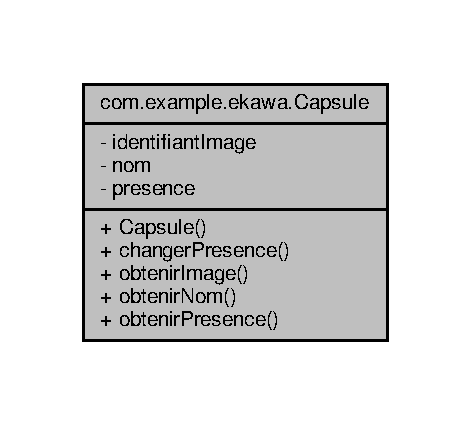
\includegraphics[width=226pt]{classcom_1_1example_1_1ekawa_1_1_capsule__coll__graph}
\end{center}
\end{figure}
\subsubsection*{Fonctions membres publiques}
\begin{DoxyCompactItemize}
\item 
\hyperlink{classcom_1_1example_1_1ekawa_1_1_capsule_a7d802ab4d4c4732063c997d1be472186}{Capsule} (String \hyperlink{classcom_1_1example_1_1ekawa_1_1_capsule_a936a082e9bcfdda4bb8fbffd33665cb0}{nom}, Integer \hyperlink{classcom_1_1example_1_1ekawa_1_1_capsule_a05fa50e416ea3a48d6b8dab73174c9d0}{identifiant\+Image}, boolean \hyperlink{classcom_1_1example_1_1ekawa_1_1_capsule_a351ef1f4b4258f4651d24b206fc38a94}{presence})
\begin{DoxyCompactList}\small\item\em Constructeur de la classe \hyperlink{classcom_1_1example_1_1ekawa_1_1_capsule}{Capsule}. \end{DoxyCompactList}\item 
void \hyperlink{classcom_1_1example_1_1ekawa_1_1_capsule_ad9c3e6efb116092fc0dfc26cf8ea6c2f}{changer\+Presence} (boolean \hyperlink{classcom_1_1example_1_1ekawa_1_1_capsule_a351ef1f4b4258f4651d24b206fc38a94}{presence})
\item 
Integer \hyperlink{classcom_1_1example_1_1ekawa_1_1_capsule_ab03475c7f750fd6319a5899da8393252}{obtenir\+Image} ()
\begin{DoxyCompactList}\small\item\em Méthode qui permet d\textquotesingle{}obtenir l\textquotesingle{}identifiant de l\textquotesingle{}image de la capsule. \end{DoxyCompactList}\item 
String \hyperlink{classcom_1_1example_1_1ekawa_1_1_capsule_a56668990154945141a80702633efc123}{obtenir\+Nom} ()
\begin{DoxyCompactList}\small\item\em Méthode qui permet d\textquotesingle{}obtenir le nom de la capsule. \end{DoxyCompactList}\item 
boolean \hyperlink{classcom_1_1example_1_1ekawa_1_1_capsule_a66a878ce2dd20d39cf49d1d66cc5c600}{obtenir\+Presence} ()
\begin{DoxyCompactList}\small\item\em Méthode qui permet d\textquotesingle{}obtenir la présence de la capsule. \end{DoxyCompactList}\end{DoxyCompactItemize}
\subsubsection*{Attributs privés}
\begin{DoxyCompactItemize}
\item 
Integer \hyperlink{classcom_1_1example_1_1ekawa_1_1_capsule_a05fa50e416ea3a48d6b8dab73174c9d0}{identifiant\+Image}
\item 
String \hyperlink{classcom_1_1example_1_1ekawa_1_1_capsule_a936a082e9bcfdda4bb8fbffd33665cb0}{nom}
\item 
boolean \hyperlink{classcom_1_1example_1_1ekawa_1_1_capsule_a351ef1f4b4258f4651d24b206fc38a94}{presence}
\end{DoxyCompactItemize}


\subsubsection{Description détaillée}
Définit les caractéristiques des capsules d\textquotesingle{}E\+K\+A\+WA. 

Définition à la ligne \hyperlink{_capsule_8java_source_l00016}{16} du fichier \hyperlink{_capsule_8java_source}{Capsule.\+java}.



\subsubsection{Documentation des constructeurs et destructeur}
\mbox{\Hypertarget{classcom_1_1example_1_1ekawa_1_1_capsule_a7d802ab4d4c4732063c997d1be472186}\label{classcom_1_1example_1_1ekawa_1_1_capsule_a7d802ab4d4c4732063c997d1be472186}} 
\index{com\+::example\+::ekawa\+::\+Capsule@{com\+::example\+::ekawa\+::\+Capsule}!Capsule@{Capsule}}
\index{Capsule@{Capsule}!com\+::example\+::ekawa\+::\+Capsule@{com\+::example\+::ekawa\+::\+Capsule}}
\paragraph{\texorpdfstring{Capsule()}{Capsule()}}
{\footnotesize\ttfamily com.\+example.\+ekawa.\+Capsule.\+Capsule (\begin{DoxyParamCaption}\item[{String}]{nom,  }\item[{Integer}]{identifiant\+Image,  }\item[{boolean}]{presence }\end{DoxyParamCaption})}



Constructeur de la classe \hyperlink{classcom_1_1example_1_1ekawa_1_1_capsule}{Capsule}. 


\begin{DoxyParams}{Paramètres}
{\em nom} & le nom de la capsule \\
\hline
{\em identifiant\+Image} & l\textquotesingle{}identifiant de l\textquotesingle{}image de la capsule \\
\hline
\end{DoxyParams}


Définition à la ligne \hyperlink{_capsule_8java_source_l00027}{27} du fichier \hyperlink{_capsule_8java_source}{Capsule.\+java}.



Références \hyperlink{_capsule_8java_source_l00019}{com.\+example.\+ekawa.\+Capsule.\+identifiant\+Image}, \hyperlink{_capsule_8java_source_l00018}{com.\+example.\+ekawa.\+Capsule.\+nom}, et \hyperlink{_capsule_8java_source_l00020}{com.\+example.\+ekawa.\+Capsule.\+presence}.


\begin{DoxyCode}
00028     \{
00029         this.\hyperlink{classcom_1_1example_1_1ekawa_1_1_capsule_a936a082e9bcfdda4bb8fbffd33665cb0}{nom} = \hyperlink{classcom_1_1example_1_1ekawa_1_1_capsule_a936a082e9bcfdda4bb8fbffd33665cb0}{nom};
00030         this.\hyperlink{classcom_1_1example_1_1ekawa_1_1_capsule_a05fa50e416ea3a48d6b8dab73174c9d0}{identifiantImage} = \hyperlink{classcom_1_1example_1_1ekawa_1_1_capsule_a05fa50e416ea3a48d6b8dab73174c9d0}{identifiantImage};
00031         this.\hyperlink{classcom_1_1example_1_1ekawa_1_1_capsule_a351ef1f4b4258f4651d24b206fc38a94}{presence} = \hyperlink{classcom_1_1example_1_1ekawa_1_1_capsule_a351ef1f4b4258f4651d24b206fc38a94}{presence};
00032     \}
\end{DoxyCode}


\subsubsection{Documentation des fonctions membres}
\mbox{\Hypertarget{classcom_1_1example_1_1ekawa_1_1_capsule_ad9c3e6efb116092fc0dfc26cf8ea6c2f}\label{classcom_1_1example_1_1ekawa_1_1_capsule_ad9c3e6efb116092fc0dfc26cf8ea6c2f}} 
\index{com\+::example\+::ekawa\+::\+Capsule@{com\+::example\+::ekawa\+::\+Capsule}!changer\+Presence@{changer\+Presence}}
\index{changer\+Presence@{changer\+Presence}!com\+::example\+::ekawa\+::\+Capsule@{com\+::example\+::ekawa\+::\+Capsule}}
\paragraph{\texorpdfstring{changer\+Presence()}{changerPresence()}}
{\footnotesize\ttfamily void com.\+example.\+ekawa.\+Capsule.\+changer\+Presence (\begin{DoxyParamCaption}\item[{boolean}]{presence }\end{DoxyParamCaption})}



Définition à la ligne \hyperlink{_capsule_8java_source_l00061}{61} du fichier \hyperlink{_capsule_8java_source}{Capsule.\+java}.



Références \hyperlink{_capsule_8java_source_l00020}{com.\+example.\+ekawa.\+Capsule.\+presence}.


\begin{DoxyCode}
00062     \{
00063         this.\hyperlink{classcom_1_1example_1_1ekawa_1_1_capsule_a351ef1f4b4258f4651d24b206fc38a94}{presence} = \hyperlink{classcom_1_1example_1_1ekawa_1_1_capsule_a351ef1f4b4258f4651d24b206fc38a94}{presence};
00064     \}
\end{DoxyCode}
\mbox{\Hypertarget{classcom_1_1example_1_1ekawa_1_1_capsule_ab03475c7f750fd6319a5899da8393252}\label{classcom_1_1example_1_1ekawa_1_1_capsule_ab03475c7f750fd6319a5899da8393252}} 
\index{com\+::example\+::ekawa\+::\+Capsule@{com\+::example\+::ekawa\+::\+Capsule}!obtenir\+Image@{obtenir\+Image}}
\index{obtenir\+Image@{obtenir\+Image}!com\+::example\+::ekawa\+::\+Capsule@{com\+::example\+::ekawa\+::\+Capsule}}
\paragraph{\texorpdfstring{obtenir\+Image()}{obtenirImage()}}
{\footnotesize\ttfamily Integer com.\+example.\+ekawa.\+Capsule.\+obtenir\+Image (\begin{DoxyParamCaption}{ }\end{DoxyParamCaption})}



Méthode qui permet d\textquotesingle{}obtenir l\textquotesingle{}identifiant de l\textquotesingle{}image de la capsule. 

\begin{DoxyReturn}{Renvoie}
Integer l\textquotesingle{}identifiant de l\textquotesingle{}image de la capsule 
\end{DoxyReturn}


Définition à la ligne \hyperlink{_capsule_8java_source_l00047}{47} du fichier \hyperlink{_capsule_8java_source}{Capsule.\+java}.



Références \hyperlink{_capsule_8java_source_l00019}{com.\+example.\+ekawa.\+Capsule.\+identifiant\+Image}.


\begin{DoxyCode}
00048     \{
00049         \textcolor{keywordflow}{return} this.\hyperlink{classcom_1_1example_1_1ekawa_1_1_capsule_a05fa50e416ea3a48d6b8dab73174c9d0}{identifiantImage};
00050     \}
\end{DoxyCode}
\mbox{\Hypertarget{classcom_1_1example_1_1ekawa_1_1_capsule_a56668990154945141a80702633efc123}\label{classcom_1_1example_1_1ekawa_1_1_capsule_a56668990154945141a80702633efc123}} 
\index{com\+::example\+::ekawa\+::\+Capsule@{com\+::example\+::ekawa\+::\+Capsule}!obtenir\+Nom@{obtenir\+Nom}}
\index{obtenir\+Nom@{obtenir\+Nom}!com\+::example\+::ekawa\+::\+Capsule@{com\+::example\+::ekawa\+::\+Capsule}}
\paragraph{\texorpdfstring{obtenir\+Nom()}{obtenirNom()}}
{\footnotesize\ttfamily String com.\+example.\+ekawa.\+Capsule.\+obtenir\+Nom (\begin{DoxyParamCaption}{ }\end{DoxyParamCaption})}



Méthode qui permet d\textquotesingle{}obtenir le nom de la capsule. 

\begin{DoxyReturn}{Renvoie}
String le nom de la capsule 
\end{DoxyReturn}


Définition à la ligne \hyperlink{_capsule_8java_source_l00038}{38} du fichier \hyperlink{_capsule_8java_source}{Capsule.\+java}.



Références \hyperlink{_capsule_8java_source_l00018}{com.\+example.\+ekawa.\+Capsule.\+nom}.


\begin{DoxyCode}
00039     \{
00040         \textcolor{keywordflow}{return} this.\hyperlink{classcom_1_1example_1_1ekawa_1_1_capsule_a936a082e9bcfdda4bb8fbffd33665cb0}{nom};
00041     \}
\end{DoxyCode}
\mbox{\Hypertarget{classcom_1_1example_1_1ekawa_1_1_capsule_a66a878ce2dd20d39cf49d1d66cc5c600}\label{classcom_1_1example_1_1ekawa_1_1_capsule_a66a878ce2dd20d39cf49d1d66cc5c600}} 
\index{com\+::example\+::ekawa\+::\+Capsule@{com\+::example\+::ekawa\+::\+Capsule}!obtenir\+Presence@{obtenir\+Presence}}
\index{obtenir\+Presence@{obtenir\+Presence}!com\+::example\+::ekawa\+::\+Capsule@{com\+::example\+::ekawa\+::\+Capsule}}
\paragraph{\texorpdfstring{obtenir\+Presence()}{obtenirPresence()}}
{\footnotesize\ttfamily boolean com.\+example.\+ekawa.\+Capsule.\+obtenir\+Presence (\begin{DoxyParamCaption}{ }\end{DoxyParamCaption})}



Méthode qui permet d\textquotesingle{}obtenir la présence de la capsule. 

\begin{DoxyReturn}{Renvoie}
boolean la présence de la capsule 
\end{DoxyReturn}


Définition à la ligne \hyperlink{_capsule_8java_source_l00056}{56} du fichier \hyperlink{_capsule_8java_source}{Capsule.\+java}.



Références \hyperlink{_capsule_8java_source_l00020}{com.\+example.\+ekawa.\+Capsule.\+presence}.


\begin{DoxyCode}
00057     \{
00058         \textcolor{keywordflow}{return} this.\hyperlink{classcom_1_1example_1_1ekawa_1_1_capsule_a351ef1f4b4258f4651d24b206fc38a94}{presence};
00059     \}
\end{DoxyCode}


\subsubsection{Documentation des données membres}
\mbox{\Hypertarget{classcom_1_1example_1_1ekawa_1_1_capsule_a05fa50e416ea3a48d6b8dab73174c9d0}\label{classcom_1_1example_1_1ekawa_1_1_capsule_a05fa50e416ea3a48d6b8dab73174c9d0}} 
\index{com\+::example\+::ekawa\+::\+Capsule@{com\+::example\+::ekawa\+::\+Capsule}!identifiant\+Image@{identifiant\+Image}}
\index{identifiant\+Image@{identifiant\+Image}!com\+::example\+::ekawa\+::\+Capsule@{com\+::example\+::ekawa\+::\+Capsule}}
\paragraph{\texorpdfstring{identifiant\+Image}{identifiantImage}}
{\footnotesize\ttfamily Integer com.\+example.\+ekawa.\+Capsule.\+identifiant\+Image\hspace{0.3cm}{\ttfamily [private]}}



Définition à la ligne \hyperlink{_capsule_8java_source_l00019}{19} du fichier \hyperlink{_capsule_8java_source}{Capsule.\+java}.



Référencé par \hyperlink{_capsule_8java_source_l00027}{com.\+example.\+ekawa.\+Capsule.\+Capsule()}, et \hyperlink{_capsule_8java_source_l00047}{com.\+example.\+ekawa.\+Capsule.\+obtenir\+Image()}.

\mbox{\Hypertarget{classcom_1_1example_1_1ekawa_1_1_capsule_a936a082e9bcfdda4bb8fbffd33665cb0}\label{classcom_1_1example_1_1ekawa_1_1_capsule_a936a082e9bcfdda4bb8fbffd33665cb0}} 
\index{com\+::example\+::ekawa\+::\+Capsule@{com\+::example\+::ekawa\+::\+Capsule}!nom@{nom}}
\index{nom@{nom}!com\+::example\+::ekawa\+::\+Capsule@{com\+::example\+::ekawa\+::\+Capsule}}
\paragraph{\texorpdfstring{nom}{nom}}
{\footnotesize\ttfamily String com.\+example.\+ekawa.\+Capsule.\+nom\hspace{0.3cm}{\ttfamily [private]}}



Définition à la ligne \hyperlink{_capsule_8java_source_l00018}{18} du fichier \hyperlink{_capsule_8java_source}{Capsule.\+java}.



Référencé par \hyperlink{_capsule_8java_source_l00027}{com.\+example.\+ekawa.\+Capsule.\+Capsule()}, et \hyperlink{_capsule_8java_source_l00038}{com.\+example.\+ekawa.\+Capsule.\+obtenir\+Nom()}.

\mbox{\Hypertarget{classcom_1_1example_1_1ekawa_1_1_capsule_a351ef1f4b4258f4651d24b206fc38a94}\label{classcom_1_1example_1_1ekawa_1_1_capsule_a351ef1f4b4258f4651d24b206fc38a94}} 
\index{com\+::example\+::ekawa\+::\+Capsule@{com\+::example\+::ekawa\+::\+Capsule}!presence@{presence}}
\index{presence@{presence}!com\+::example\+::ekawa\+::\+Capsule@{com\+::example\+::ekawa\+::\+Capsule}}
\paragraph{\texorpdfstring{presence}{presence}}
{\footnotesize\ttfamily boolean com.\+example.\+ekawa.\+Capsule.\+presence\hspace{0.3cm}{\ttfamily [private]}}



Définition à la ligne \hyperlink{_capsule_8java_source_l00020}{20} du fichier \hyperlink{_capsule_8java_source}{Capsule.\+java}.



Référencé par \hyperlink{_capsule_8java_source_l00027}{com.\+example.\+ekawa.\+Capsule.\+Capsule()}, \hyperlink{_capsule_8java_source_l00061}{com.\+example.\+ekawa.\+Capsule.\+changer\+Presence()}, et \hyperlink{_capsule_8java_source_l00056}{com.\+example.\+ekawa.\+Capsule.\+obtenir\+Presence()}.



La documentation de cette classe a été générée à partir du fichier suivant \+:\begin{DoxyCompactItemize}
\item 
\hyperlink{_capsule_8java}{Capsule.\+java}\end{DoxyCompactItemize}

\hypertarget{classcom_1_1example_1_1ekawa_1_1_communication}{}\subsection{Référence de la classe com.\+example.\+ekawa.\+Communication}
\label{classcom_1_1example_1_1ekawa_1_1_communication}\index{com.\+example.\+ekawa.\+Communication@{com.\+example.\+ekawa.\+Communication}}


Permet la communication Bluetooth avec la cafetière.  




Graphe de collaboration de com.\+example.\+ekawa.\+Communication\+:\nopagebreak
\begin{figure}[H]
\begin{center}
\leavevmode
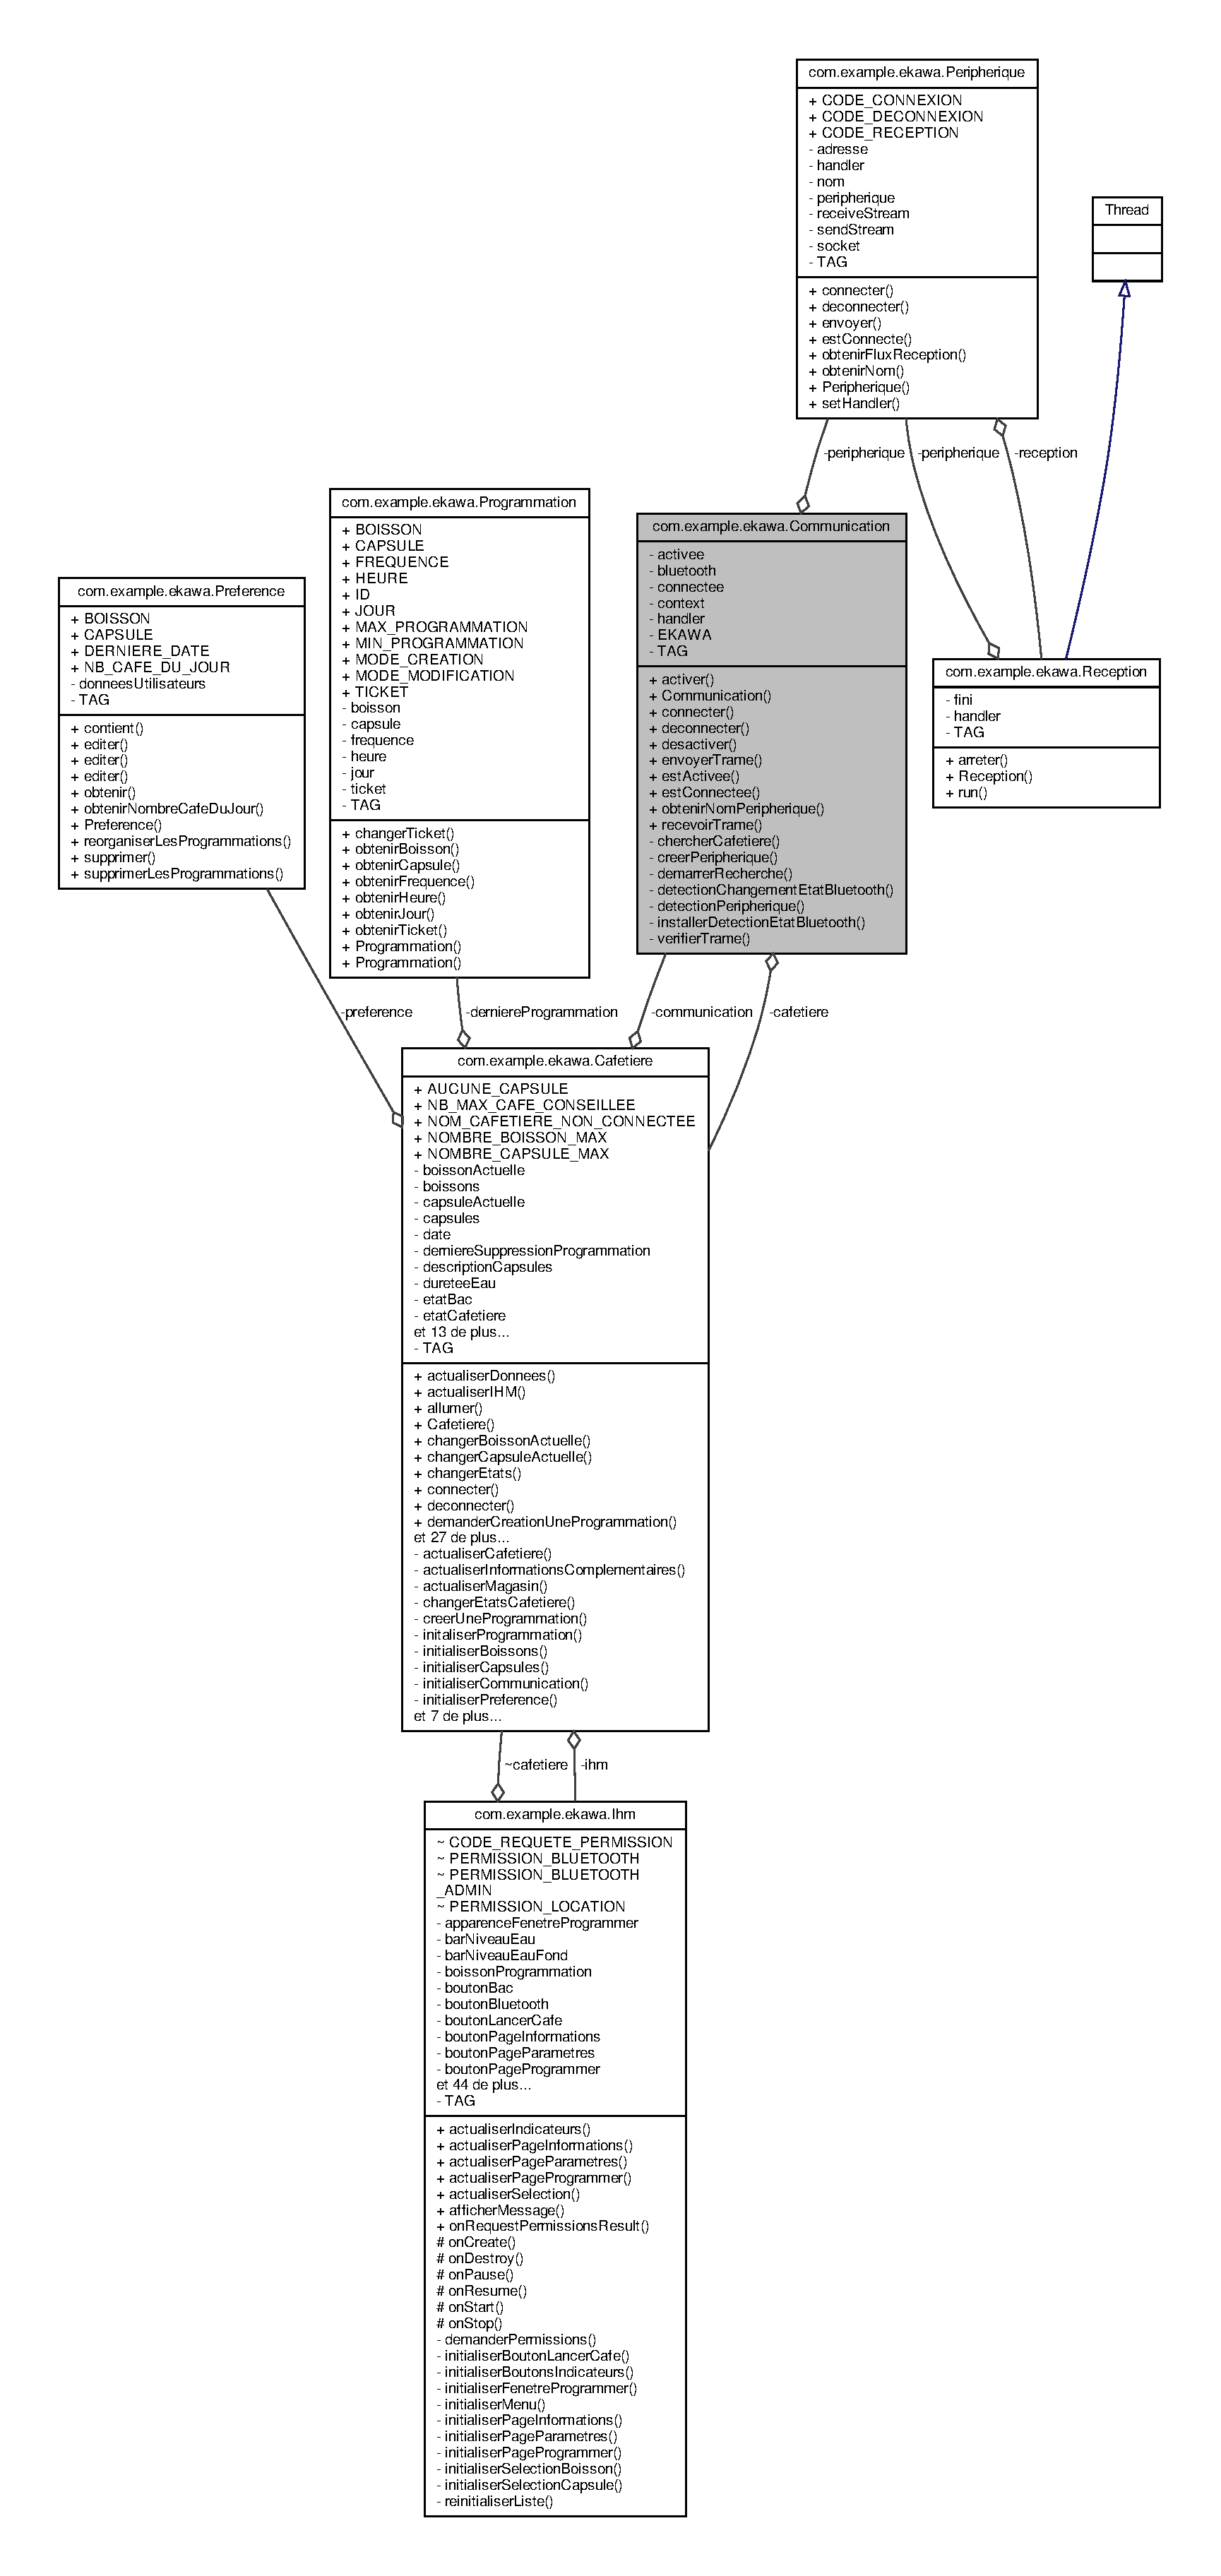
\includegraphics[height=550pt]{classcom_1_1example_1_1ekawa_1_1_communication__coll__graph}
\end{center}
\end{figure}
\subsubsection*{Fonctions membres publiques}
\begin{DoxyCompactItemize}
\item 
void \hyperlink{classcom_1_1example_1_1ekawa_1_1_communication_a64e0731414722f27a990d8ac884aca83}{activer} ()
\begin{DoxyCompactList}\small\item\em Méthode qui permet d\textquotesingle{}allumer le bluetooth. \end{DoxyCompactList}\item 
\hyperlink{classcom_1_1example_1_1ekawa_1_1_communication_a78557db29f39808417c9fa4435b90d3b}{Communication} (App\+Compat\+Activity activity, \hyperlink{classcom_1_1example_1_1ekawa_1_1_cafetiere}{Cafetiere} \hyperlink{classcom_1_1example_1_1ekawa_1_1_communication_a3b69b78cdf60bc35b2e3e564519dc1b6}{cafetiere})
\begin{DoxyCompactList}\small\item\em Constructeur de la classe \hyperlink{classcom_1_1example_1_1ekawa_1_1_communication}{Communication}. \end{DoxyCompactList}\item 
void \hyperlink{classcom_1_1example_1_1ekawa_1_1_communication_af0cb2a6a5c1674a7204174ba786e8596}{connecter} ()
\begin{DoxyCompactList}\small\item\em Méthode qui permet de connecter le bluetooth à la cafetière. \end{DoxyCompactList}\item 
void \hyperlink{classcom_1_1example_1_1ekawa_1_1_communication_a024ca42abcc8727d303a54ec44b4c99b}{deconnecter} ()
\begin{DoxyCompactList}\small\item\em Méthode qui permet de deconnecter le bluetooth de la cafetière. \end{DoxyCompactList}\item 
void \hyperlink{classcom_1_1example_1_1ekawa_1_1_communication_a230dde1900a47e26832b7467eddc556a}{desactiver} ()
\begin{DoxyCompactList}\small\item\em Méthode qui permet d\textquotesingle{}eteindre le bluetooth. \end{DoxyCompactList}\item 
void \hyperlink{classcom_1_1example_1_1ekawa_1_1_communication_a98808d0236e547b9a3ee485f66aa7af0}{envoyer\+Trame} (String trame)
\begin{DoxyCompactList}\small\item\em Méthode qui permet d\textquotesingle{}envoyer des trames à la cafetière. \end{DoxyCompactList}\item 
boolean \hyperlink{classcom_1_1example_1_1ekawa_1_1_communication_a1007662e44cb2d0af3bef6d36246bf9a}{est\+Activee} ()
\begin{DoxyCompactList}\small\item\em Méthode qui retourne si le bluetooth est activé ou non. \end{DoxyCompactList}\item 
boolean \hyperlink{classcom_1_1example_1_1ekawa_1_1_communication_a0c591a578528edaa5bb665cede5738bc}{est\+Connectee} ()
\begin{DoxyCompactList}\small\item\em Méthode qui retourne l\textquotesingle{}etat de la connection avec la cafetière. \end{DoxyCompactList}\item 
String \hyperlink{classcom_1_1example_1_1ekawa_1_1_communication_a133dd63afcf2d2f1229a416abe099494}{obtenir\+Nom\+Peripherique} ()
\begin{DoxyCompactList}\small\item\em Méthode qui retourne le nom du périphérique. \end{DoxyCompactList}\item 
String \hyperlink{classcom_1_1example_1_1ekawa_1_1_communication_a0ca98776b3fe48fa76e134607edb7871}{recevoir\+Trame} (String trame)
\begin{DoxyCompactList}\small\item\em Méthode qui permet de recevoir des trames de la cafetière. \end{DoxyCompactList}\end{DoxyCompactItemize}
\subsubsection*{Fonctions membres privées}
\begin{DoxyCompactItemize}
\item 
void \hyperlink{classcom_1_1example_1_1ekawa_1_1_communication_afc96e58f53fc167fe9fc76a229c01cb0}{chercher\+Cafetiere} ()
\begin{DoxyCompactList}\small\item\em Méthode qui permet de chercher da cafetière dans les périphérique bluetooth appareillé \end{DoxyCompactList}\item 
void \hyperlink{classcom_1_1example_1_1ekawa_1_1_communication_a41f24da10de9e598f65941bf55320566}{creer\+Peripherique} (Bluetooth\+Device \hyperlink{classcom_1_1example_1_1ekawa_1_1_communication_a59a25b4807148701560e4341f79c0c16}{peripherique})
\begin{DoxyCompactList}\small\item\em Méthode qui permet de créer le périphérique. \end{DoxyCompactList}\item 
void \hyperlink{classcom_1_1example_1_1ekawa_1_1_communication_a4b8036f1d4f4f37e15c85886af645900}{demarrer\+Recherche} ()
\begin{DoxyCompactList}\small\item\em Méthode qui permet de lancer la recherche de périphérique non appareillé \end{DoxyCompactList}\item 
final Broadcast\+Receiver \hyperlink{classcom_1_1example_1_1ekawa_1_1_communication_a7fb7acee2a343c884103481715ab4e65}{detection\+Changement\+Etat\+Bluetooth} ()
\begin{DoxyCompactList}\small\item\em Détecteur de changement d\textquotesingle{}état du bluetooth. \end{DoxyCompactList}\item 
final Broadcast\+Receiver \hyperlink{classcom_1_1example_1_1ekawa_1_1_communication_a4e46e30e8c22ae617b52260d198a76ca}{detection\+Peripherique} ()
\begin{DoxyCompactList}\small\item\em Détecteur de périphériques. \end{DoxyCompactList}\item 
void \hyperlink{classcom_1_1example_1_1ekawa_1_1_communication_a6640c878b7a4c97af7ccda45e33ead80}{installer\+Detection\+Etat\+Bluetooth} ()
\begin{DoxyCompactList}\small\item\em Méthode qui installe la détection des changements d\textquotesingle{}états bluetooth. \end{DoxyCompactList}\item 
boolean \hyperlink{classcom_1_1example_1_1ekawa_1_1_communication_a6421eb8129e103841f088870610b1b33}{verifier\+Trame} (String trame)
\begin{DoxyCompactList}\small\item\em Méthode qui permet de vérifier la trame recue. \end{DoxyCompactList}\end{DoxyCompactItemize}
\subsubsection*{Attributs privés}
\begin{DoxyCompactItemize}
\item 
boolean \hyperlink{classcom_1_1example_1_1ekawa_1_1_communication_a2f49177a9865ed41a759bce83658bb6e}{activee} = false
\begin{DoxyCompactList}\small\item\em Indique si le bluetooth est activée. \end{DoxyCompactList}\item 
Bluetooth\+Adapter \hyperlink{classcom_1_1example_1_1ekawa_1_1_communication_a0ed43f74b2eae7e8f150b049953da384}{bluetooth} = null
\begin{DoxyCompactList}\small\item\em L\textquotesingle{}adaptateur Bluetooth de la tablette. \end{DoxyCompactList}\item 
\hyperlink{classcom_1_1example_1_1ekawa_1_1_cafetiere}{Cafetiere} \hyperlink{classcom_1_1example_1_1ekawa_1_1_communication_a3b69b78cdf60bc35b2e3e564519dc1b6}{cafetiere}
\begin{DoxyCompactList}\small\item\em Relation avec l\textquotesingle{}objet principal \hyperlink{classcom_1_1example_1_1ekawa_1_1_cafetiere}{Cafetiere}. \end{DoxyCompactList}\item 
boolean \hyperlink{classcom_1_1example_1_1ekawa_1_1_communication_a93d9caaa9d4454a32d9dc28a6f22d2eb}{connectee} = false
\begin{DoxyCompactList}\small\item\em Indique l\textquotesingle{}état de la connexion avec la cafetière. \end{DoxyCompactList}\item 
Context \hyperlink{classcom_1_1example_1_1ekawa_1_1_communication_aa5ae3c4eaab6ec31d3b358431e812d00}{context}
\begin{DoxyCompactList}\small\item\em Le contexte de l\textquotesingle{}application. \end{DoxyCompactList}\item 
final Handler \hyperlink{classcom_1_1example_1_1ekawa_1_1_communication_ae1e1b4415de23491b36f0bd70da2f164}{handler}
\begin{DoxyCompactList}\small\item\em Traitement des messages en provenance des Threads. \end{DoxyCompactList}\item 
\hyperlink{classcom_1_1example_1_1ekawa_1_1_peripherique}{Peripherique} \hyperlink{classcom_1_1example_1_1ekawa_1_1_communication_a59a25b4807148701560e4341f79c0c16}{peripherique} = null
\begin{DoxyCompactList}\small\item\em Le périphérique bluetooth distant. \end{DoxyCompactList}\end{DoxyCompactItemize}
\subsubsection*{Attributs privés statiques}
\begin{DoxyCompactItemize}
\item 
static final String \hyperlink{classcom_1_1example_1_1ekawa_1_1_communication_a85da929bac3fd83864a79ed4c3a57044}{E\+K\+A\+WA} = \char`\"{}ekawa-\/\char`\"{}
\begin{DoxyCompactList}\small\item\em Nom du périphérique bluettoth. \end{DoxyCompactList}\item 
static final String \hyperlink{classcom_1_1example_1_1ekawa_1_1_communication_af355bac38153a4e6d1cda0b3e74bc1c7}{T\+AG} = \char`\"{}Communication\char`\"{}
\begin{DoxyCompactList}\small\item\em T\+AG pour les logs. \end{DoxyCompactList}\end{DoxyCompactItemize}


\subsubsection{Description détaillée}
Permet la communication Bluetooth avec la cafetière. 

Définition à la ligne \hyperlink{_communication_8java_source_l00031}{31} du fichier \hyperlink{_communication_8java_source}{Communication.\+java}.



\subsubsection{Documentation des constructeurs et destructeur}
\mbox{\Hypertarget{classcom_1_1example_1_1ekawa_1_1_communication_a78557db29f39808417c9fa4435b90d3b}\label{classcom_1_1example_1_1ekawa_1_1_communication_a78557db29f39808417c9fa4435b90d3b}} 
\index{com\+::example\+::ekawa\+::\+Communication@{com\+::example\+::ekawa\+::\+Communication}!Communication@{Communication}}
\index{Communication@{Communication}!com\+::example\+::ekawa\+::\+Communication@{com\+::example\+::ekawa\+::\+Communication}}
\paragraph{\texorpdfstring{Communication()}{Communication()}}
{\footnotesize\ttfamily com.\+example.\+ekawa.\+Communication.\+Communication (\begin{DoxyParamCaption}\item[{App\+Compat\+Activity}]{activity,  }\item[{\hyperlink{classcom_1_1example_1_1ekawa_1_1_cafetiere}{Cafetiere}}]{cafetiere }\end{DoxyParamCaption})}



Constructeur de la classe \hyperlink{classcom_1_1example_1_1ekawa_1_1_communication}{Communication}. 



Définition à la ligne \hyperlink{_communication_8java_source_l00195}{195} du fichier \hyperlink{_communication_8java_source}{Communication.\+java}.



Références \hyperlink{_communication_8java_source_l00215}{com.\+example.\+ekawa.\+Communication.\+activer()}, \hyperlink{_communication_8java_source_l00047}{com.\+example.\+ekawa.\+Communication.\+cafetiere}, et \hyperlink{_communication_8java_source_l00339}{com.\+example.\+ekawa.\+Communication.\+installer\+Detection\+Etat\+Bluetooth()}.


\begin{DoxyCode}
00196     \{
00197         Log.d(\hyperlink{classcom_1_1example_1_1ekawa_1_1_communication_af355bac38153a4e6d1cda0b3e74bc1c7}{TAG},\textcolor{stringliteral}{"Communication()"});
00198         this.\hyperlink{classcom_1_1example_1_1ekawa_1_1_communication_aa5ae3c4eaab6ec31d3b358431e812d00}{context} = activity.getApplicationContext();
00199         this.\hyperlink{classcom_1_1example_1_1ekawa_1_1_communication_a3b69b78cdf60bc35b2e3e564519dc1b6}{cafetiere} = \hyperlink{classcom_1_1example_1_1ekawa_1_1_communication_a3b69b78cdf60bc35b2e3e564519dc1b6}{cafetiere};
00200         \hyperlink{classcom_1_1example_1_1ekawa_1_1_communication_a0ed43f74b2eae7e8f150b049953da384}{bluetooth} = BluetoothAdapter.getDefaultAdapter();
00201         \textcolor{keywordflow}{if}(\hyperlink{classcom_1_1example_1_1ekawa_1_1_communication_a0ed43f74b2eae7e8f150b049953da384}{bluetooth} != null)
00202         \{
00203             \hyperlink{classcom_1_1example_1_1ekawa_1_1_communication_a6640c878b7a4c97af7ccda45e33ead80}{installerDetectionEtatBluetooth}();
00204             \hyperlink{classcom_1_1example_1_1ekawa_1_1_communication_a64e0731414722f27a990d8ac884aca83}{activer}();
00205         \}
00206         \textcolor{keywordflow}{else}
00207         \{
00208             Log.d(\hyperlink{classcom_1_1example_1_1ekawa_1_1_communication_af355bac38153a4e6d1cda0b3e74bc1c7}{TAG},\textcolor{stringliteral}{"Pas de bluetooth ?"});
00209         \}
00210     \}
\end{DoxyCode}


\subsubsection{Documentation des fonctions membres}
\mbox{\Hypertarget{classcom_1_1example_1_1ekawa_1_1_communication_a64e0731414722f27a990d8ac884aca83}\label{classcom_1_1example_1_1ekawa_1_1_communication_a64e0731414722f27a990d8ac884aca83}} 
\index{com\+::example\+::ekawa\+::\+Communication@{com\+::example\+::ekawa\+::\+Communication}!activer@{activer}}
\index{activer@{activer}!com\+::example\+::ekawa\+::\+Communication@{com\+::example\+::ekawa\+::\+Communication}}
\paragraph{\texorpdfstring{activer()}{activer()}}
{\footnotesize\ttfamily void com.\+example.\+ekawa.\+Communication.\+activer (\begin{DoxyParamCaption}{ }\end{DoxyParamCaption})}



Méthode qui permet d\textquotesingle{}allumer le bluetooth. 



Définition à la ligne \hyperlink{_communication_8java_source_l00215}{215} du fichier \hyperlink{_communication_8java_source}{Communication.\+java}.



Références \hyperlink{_communication_8java_source_l00276}{com.\+example.\+ekawa.\+Communication.\+chercher\+Cafetiere()}.



Référencé par \hyperlink{_cafetiere_8java_source_l00414}{com.\+example.\+ekawa.\+Cafetiere.\+allumer()}, et \hyperlink{_communication_8java_source_l00195}{com.\+example.\+ekawa.\+Communication.\+Communication()}.


\begin{DoxyCode}
00216     \{
00217         \textcolor{keywordflow}{if} (!\hyperlink{classcom_1_1example_1_1ekawa_1_1_communication_a0ed43f74b2eae7e8f150b049953da384}{bluetooth}.isEnabled())
00218             \hyperlink{classcom_1_1example_1_1ekawa_1_1_communication_a0ed43f74b2eae7e8f150b049953da384}{bluetooth}.enable();
00219         \hyperlink{classcom_1_1example_1_1ekawa_1_1_communication_a2f49177a9865ed41a759bce83658bb6e}{activee} = \textcolor{keyword}{true};
00220         \hyperlink{classcom_1_1example_1_1ekawa_1_1_communication_afc96e58f53fc167fe9fc76a229c01cb0}{chercherCafetiere}();
00221     \}
\end{DoxyCode}
\mbox{\Hypertarget{classcom_1_1example_1_1ekawa_1_1_communication_afc96e58f53fc167fe9fc76a229c01cb0}\label{classcom_1_1example_1_1ekawa_1_1_communication_afc96e58f53fc167fe9fc76a229c01cb0}} 
\index{com\+::example\+::ekawa\+::\+Communication@{com\+::example\+::ekawa\+::\+Communication}!chercher\+Cafetiere@{chercher\+Cafetiere}}
\index{chercher\+Cafetiere@{chercher\+Cafetiere}!com\+::example\+::ekawa\+::\+Communication@{com\+::example\+::ekawa\+::\+Communication}}
\paragraph{\texorpdfstring{chercher\+Cafetiere()}{chercherCafetiere()}}
{\footnotesize\ttfamily void com.\+example.\+ekawa.\+Communication.\+chercher\+Cafetiere (\begin{DoxyParamCaption}{ }\end{DoxyParamCaption})\hspace{0.3cm}{\ttfamily [private]}}



Méthode qui permet de chercher da cafetière dans les périphérique bluetooth appareillé 



Définition à la ligne \hyperlink{_communication_8java_source_l00276}{276} du fichier \hyperlink{_communication_8java_source}{Communication.\+java}.



Références \hyperlink{_peripherique_8java_source_l00101}{com.\+example.\+ekawa.\+Peripherique.\+connecter()}, \hyperlink{_communication_8java_source_l00365}{com.\+example.\+ekawa.\+Communication.\+creer\+Peripherique()}, \hyperlink{_communication_8java_source_l00350}{com.\+example.\+ekawa.\+Communication.\+demarrer\+Recherche()}, \hyperlink{_peripherique_8java_source_l00234}{com.\+example.\+ekawa.\+Peripherique.\+est\+Connecte()}, et \hyperlink{_peripherique_8java_source_l00244}{com.\+example.\+ekawa.\+Peripherique.\+obtenir\+Nom()}.



Référencé par \hyperlink{_communication_8java_source_l00215}{com.\+example.\+ekawa.\+Communication.\+activer()}, \hyperlink{_communication_8java_source_l00226}{com.\+example.\+ekawa.\+Communication.\+connecter()}, et \hyperlink{_communication_8java_source_l00078}{com.\+example.\+ekawa.\+Communication.\+detection\+Changement\+Etat\+Bluetooth()}.


\begin{DoxyCode}
00277     \{
00278         Set<BluetoothDevice> devices;
00279 
00280         \textcolor{keywordflow}{if}(\hyperlink{classcom_1_1example_1_1ekawa_1_1_communication_a59a25b4807148701560e4341f79c0c16}{peripherique} != null)
00281             \hyperlink{classcom_1_1example_1_1ekawa_1_1_communication_a59a25b4807148701560e4341f79c0c16}{peripherique} = null;
00282 
00283         devices = \hyperlink{classcom_1_1example_1_1ekawa_1_1_communication_a0ed43f74b2eae7e8f150b049953da384}{bluetooth}.getBondedDevices();
00284         \textcolor{keywordflow}{for}(BluetoothDevice blueDevice : devices)
00285         \{
00286             Log.d(\hyperlink{classcom_1_1example_1_1ekawa_1_1_communication_af355bac38153a4e6d1cda0b3e74bc1c7}{TAG},\textcolor{stringliteral}{"[chercherCafetiere] device : "} + blueDevice.getName() + \textcolor{stringliteral}{" ["} + blueDevice.
      getAddress() + \textcolor{stringliteral}{"]"});
00287             \textcolor{keywordflow}{if}(blueDevice.getName().startsWith(\hyperlink{classcom_1_1example_1_1ekawa_1_1_communication_a85da929bac3fd83864a79ed4c3a57044}{EKAWA}))
00288             \{
00289                 Log.d(\hyperlink{classcom_1_1example_1_1ekawa_1_1_communication_af355bac38153a4e6d1cda0b3e74bc1c7}{TAG},\textcolor{stringliteral}{"[chercherCafetiere] cafetière : "} + blueDevice.getName() + \textcolor{stringliteral}{" ["} + blueDevice.
      getAddress() + \textcolor{stringliteral}{"]"});
00290                 \hyperlink{classcom_1_1example_1_1ekawa_1_1_communication_a41f24da10de9e598f65941bf55320566}{creerPeripherique}(blueDevice);
00291                 \hyperlink{classcom_1_1example_1_1ekawa_1_1_communication_a59a25b4807148701560e4341f79c0c16}{peripherique}.\hyperlink{classcom_1_1example_1_1ekawa_1_1_peripherique_aeec8c1b360496726a5aecd6c129de81b}{connecter}();
00292                 \textcolor{keywordflow}{if}(\hyperlink{classcom_1_1example_1_1ekawa_1_1_communication_a59a25b4807148701560e4341f79c0c16}{peripherique}.\hyperlink{classcom_1_1example_1_1ekawa_1_1_peripherique_a963c20e3fba4ed926e9dee972e3b6b39}{estConnecte}())
00293                     \hyperlink{classcom_1_1example_1_1ekawa_1_1_communication_a93d9caaa9d4454a32d9dc28a6f22d2eb}{connectee} = \textcolor{keyword}{true};
00294                 Toast.makeText(\hyperlink{classcom_1_1example_1_1ekawa_1_1_communication_aa5ae3c4eaab6ec31d3b358431e812d00}{context}, \textcolor{stringliteral}{"Cafetière : "} + \hyperlink{classcom_1_1example_1_1ekawa_1_1_communication_a59a25b4807148701560e4341f79c0c16}{peripherique}.
      \hyperlink{classcom_1_1example_1_1ekawa_1_1_peripherique_ad54cfafe03dfcf18cbd9b20602c4d86e}{obtenirNom}(), Toast.LENGTH\_LONG).show();
00295                 \textcolor{keywordflow}{break};
00296             \}
00297         \}
00298 
00299         \textcolor{keywordflow}{if}(\hyperlink{classcom_1_1example_1_1ekawa_1_1_communication_a59a25b4807148701560e4341f79c0c16}{peripherique} == null)
00300         \{
00301             Log.d(\hyperlink{classcom_1_1example_1_1ekawa_1_1_communication_af355bac38153a4e6d1cda0b3e74bc1c7}{TAG},\textcolor{stringliteral}{"[chercherCafetiere] cafetière ekawa non trouvée !"});
00302             \hyperlink{classcom_1_1example_1_1ekawa_1_1_communication_a4b8036f1d4f4f37e15c85886af645900}{demarrerRecherche}();
00303         \}
00304     \}
\end{DoxyCode}
\mbox{\Hypertarget{classcom_1_1example_1_1ekawa_1_1_communication_af0cb2a6a5c1674a7204174ba786e8596}\label{classcom_1_1example_1_1ekawa_1_1_communication_af0cb2a6a5c1674a7204174ba786e8596}} 
\index{com\+::example\+::ekawa\+::\+Communication@{com\+::example\+::ekawa\+::\+Communication}!connecter@{connecter}}
\index{connecter@{connecter}!com\+::example\+::ekawa\+::\+Communication@{com\+::example\+::ekawa\+::\+Communication}}
\paragraph{\texorpdfstring{connecter()}{connecter()}}
{\footnotesize\ttfamily void com.\+example.\+ekawa.\+Communication.\+connecter (\begin{DoxyParamCaption}{ }\end{DoxyParamCaption})}



Méthode qui permet de connecter le bluetooth à la cafetière. 



Définition à la ligne \hyperlink{_communication_8java_source_l00226}{226} du fichier \hyperlink{_communication_8java_source}{Communication.\+java}.



Références \hyperlink{_communication_8java_source_l00276}{com.\+example.\+ekawa.\+Communication.\+chercher\+Cafetiere()}.



Référencé par \hyperlink{_cafetiere_8java_source_l00438}{com.\+example.\+ekawa.\+Cafetiere.\+connecter()}.


\begin{DoxyCode}
00227     \{
00228         \textcolor{keywordflow}{if}(\hyperlink{classcom_1_1example_1_1ekawa_1_1_communication_a0ed43f74b2eae7e8f150b049953da384}{bluetooth}.isEnabled())
00229         \{
00230             \hyperlink{classcom_1_1example_1_1ekawa_1_1_communication_afc96e58f53fc167fe9fc76a229c01cb0}{chercherCafetiere}();
00231         \}
00232     \}
\end{DoxyCode}
\mbox{\Hypertarget{classcom_1_1example_1_1ekawa_1_1_communication_a41f24da10de9e598f65941bf55320566}\label{classcom_1_1example_1_1ekawa_1_1_communication_a41f24da10de9e598f65941bf55320566}} 
\index{com\+::example\+::ekawa\+::\+Communication@{com\+::example\+::ekawa\+::\+Communication}!creer\+Peripherique@{creer\+Peripherique}}
\index{creer\+Peripherique@{creer\+Peripherique}!com\+::example\+::ekawa\+::\+Communication@{com\+::example\+::ekawa\+::\+Communication}}
\paragraph{\texorpdfstring{creer\+Peripherique()}{creerPeripherique()}}
{\footnotesize\ttfamily void com.\+example.\+ekawa.\+Communication.\+creer\+Peripherique (\begin{DoxyParamCaption}\item[{Bluetooth\+Device}]{peripherique }\end{DoxyParamCaption})\hspace{0.3cm}{\ttfamily [private]}}



Méthode qui permet de créer le périphérique. 



Définition à la ligne \hyperlink{_communication_8java_source_l00365}{365} du fichier \hyperlink{_communication_8java_source}{Communication.\+java}.



Référencé par \hyperlink{_communication_8java_source_l00276}{com.\+example.\+ekawa.\+Communication.\+chercher\+Cafetiere()}, et \hyperlink{_communication_8java_source_l00140}{com.\+example.\+ekawa.\+Communication.\+detection\+Peripherique()}.


\begin{DoxyCode}
00366     \{
00367         Log.d(\hyperlink{classcom_1_1example_1_1ekawa_1_1_communication_af355bac38153a4e6d1cda0b3e74bc1c7}{TAG},\textcolor{stringliteral}{"[definirPeripherique] nom : "} + \hyperlink{classcom_1_1example_1_1ekawa_1_1_communication_a59a25b4807148701560e4341f79c0c16}{peripherique}.getName());
00368         \textcolor{keywordflow}{if}(this.\hyperlink{classcom_1_1example_1_1ekawa_1_1_communication_a59a25b4807148701560e4341f79c0c16}{peripherique} != null)
00369         \{
00370             this.\hyperlink{classcom_1_1example_1_1ekawa_1_1_communication_a59a25b4807148701560e4341f79c0c16}{peripherique}.\hyperlink{classcom_1_1example_1_1ekawa_1_1_peripherique_aadfd24f4d783a7834c044041c7c035bb}{deconnecter}();
00371             this.\hyperlink{classcom_1_1example_1_1ekawa_1_1_communication_a59a25b4807148701560e4341f79c0c16}{peripherique} = null;
00372         \}
00373         this.\hyperlink{classcom_1_1example_1_1ekawa_1_1_communication_a59a25b4807148701560e4341f79c0c16}{peripherique} = \textcolor{keyword}{new} Peripherique(\hyperlink{classcom_1_1example_1_1ekawa_1_1_communication_a59a25b4807148701560e4341f79c0c16}{peripherique}, 
      \hyperlink{classcom_1_1example_1_1ekawa_1_1_communication_ae1e1b4415de23491b36f0bd70da2f164}{handler});
00374     \}
\end{DoxyCode}
\mbox{\Hypertarget{classcom_1_1example_1_1ekawa_1_1_communication_a024ca42abcc8727d303a54ec44b4c99b}\label{classcom_1_1example_1_1ekawa_1_1_communication_a024ca42abcc8727d303a54ec44b4c99b}} 
\index{com\+::example\+::ekawa\+::\+Communication@{com\+::example\+::ekawa\+::\+Communication}!deconnecter@{deconnecter}}
\index{deconnecter@{deconnecter}!com\+::example\+::ekawa\+::\+Communication@{com\+::example\+::ekawa\+::\+Communication}}
\paragraph{\texorpdfstring{deconnecter()}{deconnecter()}}
{\footnotesize\ttfamily void com.\+example.\+ekawa.\+Communication.\+deconnecter (\begin{DoxyParamCaption}{ }\end{DoxyParamCaption})}



Méthode qui permet de deconnecter le bluetooth de la cafetière. 



Définition à la ligne \hyperlink{_communication_8java_source_l00250}{250} du fichier \hyperlink{_communication_8java_source}{Communication.\+java}.



Références \hyperlink{_peripherique_8java_source_l00150}{com.\+example.\+ekawa.\+Peripherique.\+deconnecter()}.



Référencé par \hyperlink{_cafetiere_8java_source_l00448}{com.\+example.\+ekawa.\+Cafetiere.\+deconnecter()}, et \hyperlink{_communication_8java_source_l00237}{com.\+example.\+ekawa.\+Communication.\+desactiver()}.


\begin{DoxyCode}
00251     \{
00252         \textcolor{keywordflow}{if}(\hyperlink{classcom_1_1example_1_1ekawa_1_1_communication_a0ed43f74b2eae7e8f150b049953da384}{bluetooth}.isEnabled())
00253             \hyperlink{classcom_1_1example_1_1ekawa_1_1_communication_a59a25b4807148701560e4341f79c0c16}{peripherique}.\hyperlink{classcom_1_1example_1_1ekawa_1_1_peripherique_aadfd24f4d783a7834c044041c7c035bb}{deconnecter}();
00254         \hyperlink{classcom_1_1example_1_1ekawa_1_1_communication_a93d9caaa9d4454a32d9dc28a6f22d2eb}{connectee} = \textcolor{keyword}{false};
00255     \}
\end{DoxyCode}
\mbox{\Hypertarget{classcom_1_1example_1_1ekawa_1_1_communication_a4b8036f1d4f4f37e15c85886af645900}\label{classcom_1_1example_1_1ekawa_1_1_communication_a4b8036f1d4f4f37e15c85886af645900}} 
\index{com\+::example\+::ekawa\+::\+Communication@{com\+::example\+::ekawa\+::\+Communication}!demarrer\+Recherche@{demarrer\+Recherche}}
\index{demarrer\+Recherche@{demarrer\+Recherche}!com\+::example\+::ekawa\+::\+Communication@{com\+::example\+::ekawa\+::\+Communication}}
\paragraph{\texorpdfstring{demarrer\+Recherche()}{demarrerRecherche()}}
{\footnotesize\ttfamily void com.\+example.\+ekawa.\+Communication.\+demarrer\+Recherche (\begin{DoxyParamCaption}{ }\end{DoxyParamCaption})\hspace{0.3cm}{\ttfamily [private]}}



Méthode qui permet de lancer la recherche de périphérique non appareillé 



Définition à la ligne \hyperlink{_communication_8java_source_l00350}{350} du fichier \hyperlink{_communication_8java_source}{Communication.\+java}.



Références \hyperlink{_communication_8java_source_l00140}{com.\+example.\+ekawa.\+Communication.\+detection\+Peripherique()}.



Référencé par \hyperlink{_communication_8java_source_l00276}{com.\+example.\+ekawa.\+Communication.\+chercher\+Cafetiere()}.


\begin{DoxyCode}
00351     \{
00352         IntentFilter filter = \textcolor{keyword}{new} IntentFilter(BluetoothDevice.ACTION\_FOUND);
00353         filter.addAction(BluetoothAdapter.ACTION\_DISCOVERY\_STARTED);
00354         filter.addAction(BluetoothAdapter.ACTION\_DISCOVERY\_FINISHED);
00355         \hyperlink{classcom_1_1example_1_1ekawa_1_1_communication_aa5ae3c4eaab6ec31d3b358431e812d00}{context}.registerReceiver(\hyperlink{classcom_1_1example_1_1ekawa_1_1_communication_a4e46e30e8c22ae617b52260d198a76ca}{detectionPeripherique}(), filter);
00356         \textcolor{keywordflow}{if}(\hyperlink{classcom_1_1example_1_1ekawa_1_1_communication_a0ed43f74b2eae7e8f150b049953da384}{bluetooth}.isDiscovering())
00357             \hyperlink{classcom_1_1example_1_1ekawa_1_1_communication_a0ed43f74b2eae7e8f150b049953da384}{bluetooth}.cancelDiscovery();
00358         \textcolor{keywordtype}{boolean} etatDemarrageDecouverte = \hyperlink{classcom_1_1example_1_1ekawa_1_1_communication_a0ed43f74b2eae7e8f150b049953da384}{bluetooth}.startDiscovery();
00359         Log.d(\hyperlink{classcom_1_1example_1_1ekawa_1_1_communication_af355bac38153a4e6d1cda0b3e74bc1c7}{TAG},\textcolor{stringliteral}{"[chercherCafetiere] démarrage découverte bluetooth "} + etatDemarrageDecouverte);
00360     \}
\end{DoxyCode}
\mbox{\Hypertarget{classcom_1_1example_1_1ekawa_1_1_communication_a230dde1900a47e26832b7467eddc556a}\label{classcom_1_1example_1_1ekawa_1_1_communication_a230dde1900a47e26832b7467eddc556a}} 
\index{com\+::example\+::ekawa\+::\+Communication@{com\+::example\+::ekawa\+::\+Communication}!desactiver@{desactiver}}
\index{desactiver@{desactiver}!com\+::example\+::ekawa\+::\+Communication@{com\+::example\+::ekawa\+::\+Communication}}
\paragraph{\texorpdfstring{desactiver()}{desactiver()}}
{\footnotesize\ttfamily void com.\+example.\+ekawa.\+Communication.\+desactiver (\begin{DoxyParamCaption}{ }\end{DoxyParamCaption})}



Méthode qui permet d\textquotesingle{}eteindre le bluetooth. 



Définition à la ligne \hyperlink{_communication_8java_source_l00237}{237} du fichier \hyperlink{_communication_8java_source}{Communication.\+java}.



Références \hyperlink{_communication_8java_source_l00250}{com.\+example.\+ekawa.\+Communication.\+deconnecter()}.



Référencé par \hyperlink{_cafetiere_8java_source_l00424}{com.\+example.\+ekawa.\+Cafetiere.\+eteindre()}.


\begin{DoxyCode}
00238     \{
00239         \textcolor{keywordflow}{if}(\hyperlink{classcom_1_1example_1_1ekawa_1_1_communication_a0ed43f74b2eae7e8f150b049953da384}{bluetooth}.isEnabled())
00240         \{
00241             \hyperlink{classcom_1_1example_1_1ekawa_1_1_communication_a024ca42abcc8727d303a54ec44b4c99b}{deconnecter}();
00242             \hyperlink{classcom_1_1example_1_1ekawa_1_1_communication_a0ed43f74b2eae7e8f150b049953da384}{bluetooth}.disable();
00243             \hyperlink{classcom_1_1example_1_1ekawa_1_1_communication_a2f49177a9865ed41a759bce83658bb6e}{activee} = \textcolor{keyword}{false};
00244         \}
00245     \}
\end{DoxyCode}
\mbox{\Hypertarget{classcom_1_1example_1_1ekawa_1_1_communication_a7fb7acee2a343c884103481715ab4e65}\label{classcom_1_1example_1_1ekawa_1_1_communication_a7fb7acee2a343c884103481715ab4e65}} 
\index{com\+::example\+::ekawa\+::\+Communication@{com\+::example\+::ekawa\+::\+Communication}!detection\+Changement\+Etat\+Bluetooth@{detection\+Changement\+Etat\+Bluetooth}}
\index{detection\+Changement\+Etat\+Bluetooth@{detection\+Changement\+Etat\+Bluetooth}!com\+::example\+::ekawa\+::\+Communication@{com\+::example\+::ekawa\+::\+Communication}}
\paragraph{\texorpdfstring{detection\+Changement\+Etat\+Bluetooth()}{detectionChangementEtatBluetooth()}}
{\footnotesize\ttfamily final Broadcast\+Receiver com.\+example.\+ekawa.\+Communication.\+detection\+Changement\+Etat\+Bluetooth (\begin{DoxyParamCaption}{ }\end{DoxyParamCaption})\hspace{0.3cm}{\ttfamily [private]}}



Détecteur de changement d\textquotesingle{}état du bluetooth. 



Définition à la ligne \hyperlink{_communication_8java_source_l00078}{78} du fichier \hyperlink{_communication_8java_source}{Communication.\+java}.



Références \hyperlink{_cafetiere_8java_source_l00674}{com.\+example.\+ekawa.\+Cafetiere.\+actualiser\+I\+H\+M()}, \hyperlink{_communication_8java_source_l00276}{com.\+example.\+ekawa.\+Communication.\+chercher\+Cafetiere()}, \hyperlink{_peripherique_8java_source_l00101}{com.\+example.\+ekawa.\+Peripherique.\+connecter()}, \hyperlink{_peripherique_8java_source_l00234}{com.\+example.\+ekawa.\+Peripherique.\+est\+Connecte()}, et \hyperlink{_cafetiere_8java_source_l00658}{com.\+example.\+ekawa.\+Cafetiere.\+remettre\+A\+Zero()}.



Référencé par \hyperlink{_communication_8java_source_l00339}{com.\+example.\+ekawa.\+Communication.\+installer\+Detection\+Etat\+Bluetooth()}.


\begin{DoxyCode}
00079     \{
00080         BroadcastReceiver receiverEtatBluetooth = \textcolor{keyword}{new} BroadcastReceiver()
00081         \{
00082             @Override
00083             \textcolor{keyword}{public} \textcolor{keywordtype}{void} onReceive(Context \hyperlink{classcom_1_1example_1_1ekawa_1_1_communication_aa5ae3c4eaab6ec31d3b358431e812d00}{context}, Intent intent)
00084             \{
00085                 \textcolor{keyword}{final} String action = intent.getAction();
00086                 Log.d(\hyperlink{classcom_1_1example_1_1ekawa_1_1_communication_af355bac38153a4e6d1cda0b3e74bc1c7}{TAG},\textcolor{stringliteral}{"[detectionChangementEtatBluetooth] action : "} + action);
00087                 \textcolor{keywordflow}{if} (action.equals(BluetoothAdapter.ACTION\_STATE\_CHANGED))
00088                 \{
00089                     \textcolor{keyword}{final} \textcolor{keywordtype}{int} state = intent.getIntExtra(BluetoothAdapter.EXTRA\_STATE, BluetoothAdapter.
      ERROR);
00090                     \textcolor{keywordflow}{switch} (state)
00091                     \{
00092                         \textcolor{keywordflow}{case} BluetoothAdapter.STATE\_OFF:
00093                             Log.d(\hyperlink{classcom_1_1example_1_1ekawa_1_1_communication_af355bac38153a4e6d1cda0b3e74bc1c7}{TAG},\textcolor{stringliteral}{"[detectionChangementEtatBluetooth] bluetooth désactivé !"});
00094                             \hyperlink{classcom_1_1example_1_1ekawa_1_1_communication_a2f49177a9865ed41a759bce83658bb6e}{activee} = \textcolor{keyword}{false};
00095                             \hyperlink{classcom_1_1example_1_1ekawa_1_1_communication_a3b69b78cdf60bc35b2e3e564519dc1b6}{cafetiere}.\hyperlink{classcom_1_1example_1_1ekawa_1_1_cafetiere_ad8c8b7d410315f55a216de809571fd87}{actualiserIHM}();
00096                             \textcolor{keywordflow}{break};
00097                         \textcolor{keywordflow}{case} BluetoothAdapter.STATE\_TURNING\_OFF:
00098                             Log.d(\hyperlink{classcom_1_1example_1_1ekawa_1_1_communication_af355bac38153a4e6d1cda0b3e74bc1c7}{TAG},\textcolor{stringliteral}{"[detectionChangementEtatBluetooth] bluetooth en cours de
       désactivation !"});
00099                             \textcolor{keywordflow}{break};
00100                         \textcolor{keywordflow}{case} BluetoothAdapter.STATE\_ON:
00101                             Log.d(\hyperlink{classcom_1_1example_1_1ekawa_1_1_communication_af355bac38153a4e6d1cda0b3e74bc1c7}{TAG},\textcolor{stringliteral}{"[detectionChangementEtatBluetooth] bluetooth activé !"});
00102                             \hyperlink{classcom_1_1example_1_1ekawa_1_1_communication_a2f49177a9865ed41a759bce83658bb6e}{activee} = \textcolor{keyword}{true};
00103                             \hyperlink{classcom_1_1example_1_1ekawa_1_1_communication_a3b69b78cdf60bc35b2e3e564519dc1b6}{cafetiere}.\hyperlink{classcom_1_1example_1_1ekawa_1_1_cafetiere_ad8c8b7d410315f55a216de809571fd87}{actualiserIHM}();
00104                             \hyperlink{classcom_1_1example_1_1ekawa_1_1_communication_afc96e58f53fc167fe9fc76a229c01cb0}{chercherCafetiere}();
00105                             \textcolor{keywordflow}{break};
00106                         \textcolor{keywordflow}{case} BluetoothAdapter.STATE\_TURNING\_ON:
00107                             Log.d(\hyperlink{classcom_1_1example_1_1ekawa_1_1_communication_af355bac38153a4e6d1cda0b3e74bc1c7}{TAG},\textcolor{stringliteral}{"[detectionChangementEtatBluetooth] bluetooth en cours
       d'activation !"});
00108                             \textcolor{keywordflow}{break};
00109                         \textcolor{keywordflow}{default}:
00110                             Log.d(\hyperlink{classcom_1_1example_1_1ekawa_1_1_communication_af355bac38153a4e6d1cda0b3e74bc1c7}{TAG},\textcolor{stringliteral}{"[detectionChangementEtatBluetooth] etat : "} + state);
00111                             \textcolor{keywordflow}{break};
00112                     \}
00113                 \}
00114                 \textcolor{keywordflow}{else} \textcolor{keywordflow}{if} (action.equals(BluetoothDevice.ACTION\_ACL\_DISCONNECTED))
00115                 \{
00116                     Log.d(\hyperlink{classcom_1_1example_1_1ekawa_1_1_communication_af355bac38153a4e6d1cda0b3e74bc1c7}{TAG},\textcolor{stringliteral}{"[detectionChangementEtatBluetooth] bluetooth déconnecté !"});
00117                     \hyperlink{classcom_1_1example_1_1ekawa_1_1_communication_a93d9caaa9d4454a32d9dc28a6f22d2eb}{connectee} = \textcolor{keyword}{false};
00118                     \hyperlink{classcom_1_1example_1_1ekawa_1_1_communication_a3b69b78cdf60bc35b2e3e564519dc1b6}{cafetiere}.\hyperlink{classcom_1_1example_1_1ekawa_1_1_cafetiere_a10a040b45cfaac52cd5c26049bf2d7b7}{remettreAZero}();
00119                 \}
00120                 \textcolor{keywordflow}{else} \textcolor{keywordflow}{if}(action.equals(BluetoothDevice.ACTION\_BOND\_STATE\_CHANGED))
00121                 \{
00122                     \textcolor{keyword}{final} \textcolor{keywordtype}{int} state = intent.getIntExtra(BluetoothDevice.EXTRA\_BOND\_STATE, BluetoothAdapter
      .ERROR);
00123                     \textcolor{keywordflow}{if}(state == BluetoothDevice.BOND\_BONDED)
00124                     \{
00125                         Log.d(\hyperlink{classcom_1_1example_1_1ekawa_1_1_communication_af355bac38153a4e6d1cda0b3e74bc1c7}{TAG},\textcolor{stringliteral}{"[detectionChangementEtatBluetooth] cafetière appairée !"});
00126                         \hyperlink{classcom_1_1example_1_1ekawa_1_1_communication_a59a25b4807148701560e4341f79c0c16}{peripherique}.\hyperlink{classcom_1_1example_1_1ekawa_1_1_peripherique_aeec8c1b360496726a5aecd6c129de81b}{connecter}();
00127                         \textcolor{keywordflow}{if}(\hyperlink{classcom_1_1example_1_1ekawa_1_1_communication_a59a25b4807148701560e4341f79c0c16}{peripherique}.\hyperlink{classcom_1_1example_1_1ekawa_1_1_peripherique_a963c20e3fba4ed926e9dee972e3b6b39}{estConnecte}())
00128                             \hyperlink{classcom_1_1example_1_1ekawa_1_1_communication_a93d9caaa9d4454a32d9dc28a6f22d2eb}{connectee} = \textcolor{keyword}{true};
00129                     \}
00130                 \}
00131             \}
00132         \};
00133 
00134         \textcolor{keywordflow}{return} receiverEtatBluetooth;
00135     \}
\end{DoxyCode}
\mbox{\Hypertarget{classcom_1_1example_1_1ekawa_1_1_communication_a4e46e30e8c22ae617b52260d198a76ca}\label{classcom_1_1example_1_1ekawa_1_1_communication_a4e46e30e8c22ae617b52260d198a76ca}} 
\index{com\+::example\+::ekawa\+::\+Communication@{com\+::example\+::ekawa\+::\+Communication}!detection\+Peripherique@{detection\+Peripherique}}
\index{detection\+Peripherique@{detection\+Peripherique}!com\+::example\+::ekawa\+::\+Communication@{com\+::example\+::ekawa\+::\+Communication}}
\paragraph{\texorpdfstring{detection\+Peripherique()}{detectionPeripherique()}}
{\footnotesize\ttfamily final Broadcast\+Receiver com.\+example.\+ekawa.\+Communication.\+detection\+Peripherique (\begin{DoxyParamCaption}{ }\end{DoxyParamCaption})\hspace{0.3cm}{\ttfamily [private]}}



Détecteur de périphériques. 



Définition à la ligne \hyperlink{_communication_8java_source_l00140}{140} du fichier \hyperlink{_communication_8java_source}{Communication.\+java}.



Références \hyperlink{_communication_8java_source_l00365}{com.\+example.\+ekawa.\+Communication.\+creer\+Peripherique()}.



Référencé par \hyperlink{_communication_8java_source_l00350}{com.\+example.\+ekawa.\+Communication.\+demarrer\+Recherche()}.


\begin{DoxyCode}
00141     \{
00142         BroadcastReceiver receiverDetectionBluetooth = \textcolor{keyword}{new} BroadcastReceiver()
00143         \{
00144             \textcolor{keyword}{public} \textcolor{keywordtype}{void} onReceive(Context \hyperlink{classcom_1_1example_1_1ekawa_1_1_communication_aa5ae3c4eaab6ec31d3b358431e812d00}{context}, Intent intent)
00145             \{
00146                 \textcolor{keywordtype}{boolean} appaire = \textcolor{keyword}{false};
00147 
00148                 String action = intent.getAction();
00149                 Log.d(\hyperlink{classcom_1_1example_1_1ekawa_1_1_communication_af355bac38153a4e6d1cda0b3e74bc1c7}{TAG}, \textcolor{stringliteral}{"[receiverDetectionBluetooth] action : "} + action);
00150 
00151                 \textcolor{keywordflow}{if} (BluetoothAdapter.ACTION\_DISCOVERY\_STARTED.equals(action))
00152                 \{
00153                     Log.d(\hyperlink{classcom_1_1example_1_1ekawa_1_1_communication_af355bac38153a4e6d1cda0b3e74bc1c7}{TAG}, \textcolor{stringliteral}{"[receiverDetectionBluetooth] découverte démarrée"});
00154                 \}
00155                 \textcolor{keywordflow}{else} \textcolor{keywordflow}{if} (BluetoothAdapter.ACTION\_DISCOVERY\_FINISHED.equals(action))
00156                 \{
00157                     Log.d(\hyperlink{classcom_1_1example_1_1ekawa_1_1_communication_af355bac38153a4e6d1cda0b3e74bc1c7}{TAG}, \textcolor{stringliteral}{"[receiverDetectionBluetooth] découverte terminée"});
00158                 \}
00159                 \textcolor{keywordflow}{else} \textcolor{keywordflow}{if} (BluetoothDevice.ACTION\_FOUND.equals(action))
00160                 \{
00161                     BluetoothDevice device = intent.getParcelableExtra(BluetoothDevice.EXTRA\_DEVICE);
00162                     Log.d(\hyperlink{classcom_1_1example_1_1ekawa_1_1_communication_af355bac38153a4e6d1cda0b3e74bc1c7}{TAG},\textcolor{stringliteral}{"[receiverDetectionBluetooth] device détecté : "} + device.getName() + \textcolor{stringliteral}{" ["}
       + device.getAddress() + \textcolor{stringliteral}{"]"});
00163                     \textcolor{keywordflow}{if} (device.getName() != null && device.getName().startsWith(
      \hyperlink{classcom_1_1example_1_1ekawa_1_1_communication_a85da929bac3fd83864a79ed4c3a57044}{EKAWA}))
00164                     \{
00165                         Toast.makeText(context, \textcolor{stringliteral}{"Trouvé : "} + device.getName(), Toast.LENGTH\_LONG).show();
00166                         \textcolor{keywordflow}{if} (device.getBondState() != BluetoothDevice.BOND\_BONDED)
00167                         \{
00168                             Log.d(\hyperlink{classcom_1_1example_1_1ekawa_1_1_communication_af355bac38153a4e6d1cda0b3e74bc1c7}{TAG},\textcolor{stringliteral}{"[receiverDetectionBluetooth] cafetière détectée mais non appairée
       !"});
00169                             \textcolor{keywordflow}{if}(Build.VERSION.SDK\_INT >= 19)
00170                             \{
00171                                 appaire = device.createBond(); \textcolor{comment}{// appairage}
00172                             \}
00173                             \textcolor{keywordflow}{else}
00174                             \{
00175                                 Toast.makeText(context, \textcolor{stringliteral}{"Veuillez associer votre cafetière Ekawa au
       bluetooth manuellement."}, Toast.LENGTH\_LONG).show();
00176                             \}
00177                         \}
00178                         \textcolor{keywordflow}{if} (device.getBondState() == BluetoothDevice.BOND\_BONDED || appaire)
00179                         \{
00180                             Log.d(\hyperlink{classcom_1_1example_1_1ekawa_1_1_communication_af355bac38153a4e6d1cda0b3e74bc1c7}{TAG}, \textcolor{stringliteral}{"[receiverDetectionBluetooth] cafetière appairée : "} + device.
      getName() + \textcolor{stringliteral}{" ["} + device.getAddress() + \textcolor{stringliteral}{"]"});
00181                             \hyperlink{classcom_1_1example_1_1ekawa_1_1_communication_a41f24da10de9e598f65941bf55320566}{creerPeripherique}(device);
00182                             \hyperlink{classcom_1_1example_1_1ekawa_1_1_communication_a0ed43f74b2eae7e8f150b049953da384}{bluetooth}.cancelDiscovery();
00183                         \}
00184                     \}
00185                 \}
00186             \}
00187         \};
00188 
00189         \textcolor{keywordflow}{return} receiverDetectionBluetooth;
00190     \};
\end{DoxyCode}
\mbox{\Hypertarget{classcom_1_1example_1_1ekawa_1_1_communication_a98808d0236e547b9a3ee485f66aa7af0}\label{classcom_1_1example_1_1ekawa_1_1_communication_a98808d0236e547b9a3ee485f66aa7af0}} 
\index{com\+::example\+::ekawa\+::\+Communication@{com\+::example\+::ekawa\+::\+Communication}!envoyer\+Trame@{envoyer\+Trame}}
\index{envoyer\+Trame@{envoyer\+Trame}!com\+::example\+::ekawa\+::\+Communication@{com\+::example\+::ekawa\+::\+Communication}}
\paragraph{\texorpdfstring{envoyer\+Trame()}{envoyerTrame()}}
{\footnotesize\ttfamily void com.\+example.\+ekawa.\+Communication.\+envoyer\+Trame (\begin{DoxyParamCaption}\item[{String}]{trame }\end{DoxyParamCaption})}



Méthode qui permet d\textquotesingle{}envoyer des trames à la cafetière. 



Définition à la ligne \hyperlink{_communication_8java_source_l00309}{309} du fichier \hyperlink{_communication_8java_source}{Communication.\+java}.



Références \hyperlink{_peripherique_8java_source_l00197}{com.\+example.\+ekawa.\+Peripherique.\+envoyer()}.



Référencé par \hyperlink{_cafetiere_8java_source_l00495}{com.\+example.\+ekawa.\+Cafetiere.\+actualiser\+Donnees()}, \hyperlink{_cafetiere_8java_source_l00720}{com.\+example.\+ekawa.\+Cafetiere.\+demander\+Creation\+Une\+Programmation()}, \hyperlink{_cafetiere_8java_source_l00397}{com.\+example.\+ekawa.\+Cafetiere.\+demander\+Preparation\+Cafe()}, \hyperlink{_cafetiere_8java_source_l00793}{com.\+example.\+ekawa.\+Cafetiere.\+demander\+Suppression\+Une\+Programmation()}, et \hyperlink{_cafetiere_8java_source_l00683}{com.\+example.\+ekawa.\+Cafetiere.\+reinitialiser\+Informations()}.


\begin{DoxyCode}
00310     \{
00311         \textcolor{keywordflow}{if}(\hyperlink{classcom_1_1example_1_1ekawa_1_1_communication_a59a25b4807148701560e4341f79c0c16}{peripherique} != null)
00312             \hyperlink{classcom_1_1example_1_1ekawa_1_1_communication_a59a25b4807148701560e4341f79c0c16}{peripherique}.\hyperlink{classcom_1_1example_1_1ekawa_1_1_peripherique_ac1361bc1a445b00c4c7ebb56dfee274d}{envoyer}(trame);
00313     \}
\end{DoxyCode}
\mbox{\Hypertarget{classcom_1_1example_1_1ekawa_1_1_communication_a1007662e44cb2d0af3bef6d36246bf9a}\label{classcom_1_1example_1_1ekawa_1_1_communication_a1007662e44cb2d0af3bef6d36246bf9a}} 
\index{com\+::example\+::ekawa\+::\+Communication@{com\+::example\+::ekawa\+::\+Communication}!est\+Activee@{est\+Activee}}
\index{est\+Activee@{est\+Activee}!com\+::example\+::ekawa\+::\+Communication@{com\+::example\+::ekawa\+::\+Communication}}
\paragraph{\texorpdfstring{est\+Activee()}{estActivee()}}
{\footnotesize\ttfamily boolean com.\+example.\+ekawa.\+Communication.\+est\+Activee (\begin{DoxyParamCaption}{ }\end{DoxyParamCaption})}



Méthode qui retourne si le bluetooth est activé ou non. 



Définition à la ligne \hyperlink{_communication_8java_source_l00268}{268} du fichier \hyperlink{_communication_8java_source}{Communication.\+java}.



Références \hyperlink{_communication_8java_source_l00042}{com.\+example.\+ekawa.\+Communication.\+activee}.



Référencé par \hyperlink{_cafetiere_8java_source_l00636}{com.\+example.\+ekawa.\+Cafetiere.\+changer\+Etats\+Cafetiere()}, et \hyperlink{_cafetiere_8java_source_l00265}{com.\+example.\+ekawa.\+Cafetiere.\+informer\+Etat\+Bluetooth()}.


\begin{DoxyCode}
00269     \{
00270         \textcolor{keywordflow}{return} \hyperlink{classcom_1_1example_1_1ekawa_1_1_communication_a2f49177a9865ed41a759bce83658bb6e}{activee};
00271     \}
\end{DoxyCode}
\mbox{\Hypertarget{classcom_1_1example_1_1ekawa_1_1_communication_a0c591a578528edaa5bb665cede5738bc}\label{classcom_1_1example_1_1ekawa_1_1_communication_a0c591a578528edaa5bb665cede5738bc}} 
\index{com\+::example\+::ekawa\+::\+Communication@{com\+::example\+::ekawa\+::\+Communication}!est\+Connectee@{est\+Connectee}}
\index{est\+Connectee@{est\+Connectee}!com\+::example\+::ekawa\+::\+Communication@{com\+::example\+::ekawa\+::\+Communication}}
\paragraph{\texorpdfstring{est\+Connectee()}{estConnectee()}}
{\footnotesize\ttfamily boolean com.\+example.\+ekawa.\+Communication.\+est\+Connectee (\begin{DoxyParamCaption}{ }\end{DoxyParamCaption})}



Méthode qui retourne l\textquotesingle{}etat de la connection avec la cafetière. 



Définition à la ligne \hyperlink{_communication_8java_source_l00260}{260} du fichier \hyperlink{_communication_8java_source}{Communication.\+java}.



Références \hyperlink{_communication_8java_source_l00043}{com.\+example.\+ekawa.\+Communication.\+connectee}.



Référencé par \hyperlink{_cafetiere_8java_source_l00495}{com.\+example.\+ekawa.\+Cafetiere.\+actualiser\+Donnees()}, \hyperlink{_cafetiere_8java_source_l00636}{com.\+example.\+ekawa.\+Cafetiere.\+changer\+Etats\+Cafetiere()}, \hyperlink{_cafetiere_8java_source_l00275}{com.\+example.\+ekawa.\+Cafetiere.\+informer\+Connexion\+Bluetooth()}, et \hyperlink{_cafetiere_8java_source_l00336}{com.\+example.\+ekawa.\+Cafetiere.\+informer\+Nom\+Cafetiere()}.


\begin{DoxyCode}
00261     \{
00262         \textcolor{keywordflow}{return} \hyperlink{classcom_1_1example_1_1ekawa_1_1_communication_a93d9caaa9d4454a32d9dc28a6f22d2eb}{connectee};
00263     \}
\end{DoxyCode}
\mbox{\Hypertarget{classcom_1_1example_1_1ekawa_1_1_communication_a6640c878b7a4c97af7ccda45e33ead80}\label{classcom_1_1example_1_1ekawa_1_1_communication_a6640c878b7a4c97af7ccda45e33ead80}} 
\index{com\+::example\+::ekawa\+::\+Communication@{com\+::example\+::ekawa\+::\+Communication}!installer\+Detection\+Etat\+Bluetooth@{installer\+Detection\+Etat\+Bluetooth}}
\index{installer\+Detection\+Etat\+Bluetooth@{installer\+Detection\+Etat\+Bluetooth}!com\+::example\+::ekawa\+::\+Communication@{com\+::example\+::ekawa\+::\+Communication}}
\paragraph{\texorpdfstring{installer\+Detection\+Etat\+Bluetooth()}{installerDetectionEtatBluetooth()}}
{\footnotesize\ttfamily void com.\+example.\+ekawa.\+Communication.\+installer\+Detection\+Etat\+Bluetooth (\begin{DoxyParamCaption}{ }\end{DoxyParamCaption})\hspace{0.3cm}{\ttfamily [private]}}



Méthode qui installe la détection des changements d\textquotesingle{}états bluetooth. 



Définition à la ligne \hyperlink{_communication_8java_source_l00339}{339} du fichier \hyperlink{_communication_8java_source}{Communication.\+java}.



Références \hyperlink{_communication_8java_source_l00078}{com.\+example.\+ekawa.\+Communication.\+detection\+Changement\+Etat\+Bluetooth()}.



Référencé par \hyperlink{_communication_8java_source_l00195}{com.\+example.\+ekawa.\+Communication.\+Communication()}.


\begin{DoxyCode}
00340     \{
00341         IntentFilter filter = \textcolor{keyword}{new} IntentFilter(BluetoothAdapter.ACTION\_STATE\_CHANGED);
00342         filter.addAction(BluetoothDevice.ACTION\_ACL\_DISCONNECTED);
00343         filter.addAction(BluetoothDevice.ACTION\_BOND\_STATE\_CHANGED);
00344         \hyperlink{classcom_1_1example_1_1ekawa_1_1_communication_aa5ae3c4eaab6ec31d3b358431e812d00}{context}.registerReceiver(\hyperlink{classcom_1_1example_1_1ekawa_1_1_communication_a7fb7acee2a343c884103481715ab4e65}{detectionChangementEtatBluetooth}(),
       filter);
00345     \}
\end{DoxyCode}
\mbox{\Hypertarget{classcom_1_1example_1_1ekawa_1_1_communication_a133dd63afcf2d2f1229a416abe099494}\label{classcom_1_1example_1_1ekawa_1_1_communication_a133dd63afcf2d2f1229a416abe099494}} 
\index{com\+::example\+::ekawa\+::\+Communication@{com\+::example\+::ekawa\+::\+Communication}!obtenir\+Nom\+Peripherique@{obtenir\+Nom\+Peripherique}}
\index{obtenir\+Nom\+Peripherique@{obtenir\+Nom\+Peripherique}!com\+::example\+::ekawa\+::\+Communication@{com\+::example\+::ekawa\+::\+Communication}}
\paragraph{\texorpdfstring{obtenir\+Nom\+Peripherique()}{obtenirNomPeripherique()}}
{\footnotesize\ttfamily String com.\+example.\+ekawa.\+Communication.\+obtenir\+Nom\+Peripherique (\begin{DoxyParamCaption}{ }\end{DoxyParamCaption})}



Méthode qui retourne le nom du périphérique. 



Définition à la ligne \hyperlink{_communication_8java_source_l00379}{379} du fichier \hyperlink{_communication_8java_source}{Communication.\+java}.



Références \hyperlink{_peripherique_8java_source_l00244}{com.\+example.\+ekawa.\+Peripherique.\+obtenir\+Nom()}.



Référencé par \hyperlink{_cafetiere_8java_source_l00336}{com.\+example.\+ekawa.\+Cafetiere.\+informer\+Nom\+Cafetiere()}.


\begin{DoxyCode}
00380     \{
00381         \textcolor{keywordflow}{if}(\hyperlink{classcom_1_1example_1_1ekawa_1_1_communication_a59a25b4807148701560e4341f79c0c16}{peripherique} != null)
00382             \textcolor{keywordflow}{return} \hyperlink{classcom_1_1example_1_1ekawa_1_1_communication_a59a25b4807148701560e4341f79c0c16}{peripherique}.\hyperlink{classcom_1_1example_1_1ekawa_1_1_peripherique_ad54cfafe03dfcf18cbd9b20602c4d86e}{obtenirNom}();
00383         \textcolor{keywordflow}{return} null;
00384     \}
\end{DoxyCode}
\mbox{\Hypertarget{classcom_1_1example_1_1ekawa_1_1_communication_a0ca98776b3fe48fa76e134607edb7871}\label{classcom_1_1example_1_1ekawa_1_1_communication_a0ca98776b3fe48fa76e134607edb7871}} 
\index{com\+::example\+::ekawa\+::\+Communication@{com\+::example\+::ekawa\+::\+Communication}!recevoir\+Trame@{recevoir\+Trame}}
\index{recevoir\+Trame@{recevoir\+Trame}!com\+::example\+::ekawa\+::\+Communication@{com\+::example\+::ekawa\+::\+Communication}}
\paragraph{\texorpdfstring{recevoir\+Trame()}{recevoirTrame()}}
{\footnotesize\ttfamily String com.\+example.\+ekawa.\+Communication.\+recevoir\+Trame (\begin{DoxyParamCaption}\item[{String}]{trame }\end{DoxyParamCaption})}



Méthode qui permet de recevoir des trames de la cafetière. 



Définition à la ligne \hyperlink{_communication_8java_source_l00318}{318} du fichier \hyperlink{_communication_8java_source}{Communication.\+java}.



Références \hyperlink{_communication_8java_source_l00329}{com.\+example.\+ekawa.\+Communication.\+verifier\+Trame()}.


\begin{DoxyCode}
00319     \{
00320         Log.d(\hyperlink{classcom_1_1example_1_1ekawa_1_1_communication_af355bac38153a4e6d1cda0b3e74bc1c7}{TAG},\textcolor{stringliteral}{"Recu : "} + trame);
00321         \textcolor{keywordflow}{if}(\hyperlink{classcom_1_1example_1_1ekawa_1_1_communication_a6421eb8129e103841f088870610b1b33}{verifierTrame}(trame))
00322             \textcolor{keywordflow}{return} trame;
00323         \textcolor{keywordflow}{return} null;
00324     \}
\end{DoxyCode}
\mbox{\Hypertarget{classcom_1_1example_1_1ekawa_1_1_communication_a6421eb8129e103841f088870610b1b33}\label{classcom_1_1example_1_1ekawa_1_1_communication_a6421eb8129e103841f088870610b1b33}} 
\index{com\+::example\+::ekawa\+::\+Communication@{com\+::example\+::ekawa\+::\+Communication}!verifier\+Trame@{verifier\+Trame}}
\index{verifier\+Trame@{verifier\+Trame}!com\+::example\+::ekawa\+::\+Communication@{com\+::example\+::ekawa\+::\+Communication}}
\paragraph{\texorpdfstring{verifier\+Trame()}{verifierTrame()}}
{\footnotesize\ttfamily boolean com.\+example.\+ekawa.\+Communication.\+verifier\+Trame (\begin{DoxyParamCaption}\item[{String}]{trame }\end{DoxyParamCaption})\hspace{0.3cm}{\ttfamily [private]}}



Méthode qui permet de vérifier la trame recue. 



Définition à la ligne \hyperlink{_communication_8java_source_l00329}{329} du fichier \hyperlink{_communication_8java_source}{Communication.\+java}.



Références \hyperlink{_protocole_8java_source_l00025}{com.\+example.\+ekawa.\+Protocole.\+D\+E\+B\+U\+T\+\_\+\+T\+R\+A\+ME}.



Référencé par \hyperlink{_communication_8java_source_l00318}{com.\+example.\+ekawa.\+Communication.\+recevoir\+Trame()}.


\begin{DoxyCode}
00330     \{
00331         \textcolor{keywordflow}{if}(trame.startsWith(Protocole.DEBUT\_TRAME))
00332             \textcolor{keywordflow}{return} \textcolor{keyword}{true};
00333         \textcolor{keywordflow}{return} \textcolor{keyword}{false};
00334     \}
\end{DoxyCode}


\subsubsection{Documentation des données membres}
\mbox{\Hypertarget{classcom_1_1example_1_1ekawa_1_1_communication_a2f49177a9865ed41a759bce83658bb6e}\label{classcom_1_1example_1_1ekawa_1_1_communication_a2f49177a9865ed41a759bce83658bb6e}} 
\index{com\+::example\+::ekawa\+::\+Communication@{com\+::example\+::ekawa\+::\+Communication}!activee@{activee}}
\index{activee@{activee}!com\+::example\+::ekawa\+::\+Communication@{com\+::example\+::ekawa\+::\+Communication}}
\paragraph{\texorpdfstring{activee}{activee}}
{\footnotesize\ttfamily boolean com.\+example.\+ekawa.\+Communication.\+activee = false\hspace{0.3cm}{\ttfamily [private]}}



Indique si le bluetooth est activée. 

Attributs 

Définition à la ligne \hyperlink{_communication_8java_source_l00042}{42} du fichier \hyperlink{_communication_8java_source}{Communication.\+java}.



Référencé par \hyperlink{_communication_8java_source_l00268}{com.\+example.\+ekawa.\+Communication.\+est\+Activee()}.

\mbox{\Hypertarget{classcom_1_1example_1_1ekawa_1_1_communication_a0ed43f74b2eae7e8f150b049953da384}\label{classcom_1_1example_1_1ekawa_1_1_communication_a0ed43f74b2eae7e8f150b049953da384}} 
\index{com\+::example\+::ekawa\+::\+Communication@{com\+::example\+::ekawa\+::\+Communication}!bluetooth@{bluetooth}}
\index{bluetooth@{bluetooth}!com\+::example\+::ekawa\+::\+Communication@{com\+::example\+::ekawa\+::\+Communication}}
\paragraph{\texorpdfstring{bluetooth}{bluetooth}}
{\footnotesize\ttfamily Bluetooth\+Adapter com.\+example.\+ekawa.\+Communication.\+bluetooth = null\hspace{0.3cm}{\ttfamily [private]}}



L\textquotesingle{}adaptateur Bluetooth de la tablette. 



Définition à la ligne \hyperlink{_communication_8java_source_l00044}{44} du fichier \hyperlink{_communication_8java_source}{Communication.\+java}.

\mbox{\Hypertarget{classcom_1_1example_1_1ekawa_1_1_communication_a3b69b78cdf60bc35b2e3e564519dc1b6}\label{classcom_1_1example_1_1ekawa_1_1_communication_a3b69b78cdf60bc35b2e3e564519dc1b6}} 
\index{com\+::example\+::ekawa\+::\+Communication@{com\+::example\+::ekawa\+::\+Communication}!cafetiere@{cafetiere}}
\index{cafetiere@{cafetiere}!com\+::example\+::ekawa\+::\+Communication@{com\+::example\+::ekawa\+::\+Communication}}
\paragraph{\texorpdfstring{cafetiere}{cafetiere}}
{\footnotesize\ttfamily \hyperlink{classcom_1_1example_1_1ekawa_1_1_cafetiere}{Cafetiere} com.\+example.\+ekawa.\+Communication.\+cafetiere\hspace{0.3cm}{\ttfamily [private]}}



Relation avec l\textquotesingle{}objet principal \hyperlink{classcom_1_1example_1_1ekawa_1_1_cafetiere}{Cafetiere}. 



Définition à la ligne \hyperlink{_communication_8java_source_l00047}{47} du fichier \hyperlink{_communication_8java_source}{Communication.\+java}.



Référencé par \hyperlink{_communication_8java_source_l00195}{com.\+example.\+ekawa.\+Communication.\+Communication()}.

\mbox{\Hypertarget{classcom_1_1example_1_1ekawa_1_1_communication_a93d9caaa9d4454a32d9dc28a6f22d2eb}\label{classcom_1_1example_1_1ekawa_1_1_communication_a93d9caaa9d4454a32d9dc28a6f22d2eb}} 
\index{com\+::example\+::ekawa\+::\+Communication@{com\+::example\+::ekawa\+::\+Communication}!connectee@{connectee}}
\index{connectee@{connectee}!com\+::example\+::ekawa\+::\+Communication@{com\+::example\+::ekawa\+::\+Communication}}
\paragraph{\texorpdfstring{connectee}{connectee}}
{\footnotesize\ttfamily boolean com.\+example.\+ekawa.\+Communication.\+connectee = false\hspace{0.3cm}{\ttfamily [private]}}



Indique l\textquotesingle{}état de la connexion avec la cafetière. 



Définition à la ligne \hyperlink{_communication_8java_source_l00043}{43} du fichier \hyperlink{_communication_8java_source}{Communication.\+java}.



Référencé par \hyperlink{_communication_8java_source_l00260}{com.\+example.\+ekawa.\+Communication.\+est\+Connectee()}.

\mbox{\Hypertarget{classcom_1_1example_1_1ekawa_1_1_communication_aa5ae3c4eaab6ec31d3b358431e812d00}\label{classcom_1_1example_1_1ekawa_1_1_communication_aa5ae3c4eaab6ec31d3b358431e812d00}} 
\index{com\+::example\+::ekawa\+::\+Communication@{com\+::example\+::ekawa\+::\+Communication}!context@{context}}
\index{context@{context}!com\+::example\+::ekawa\+::\+Communication@{com\+::example\+::ekawa\+::\+Communication}}
\paragraph{\texorpdfstring{context}{context}}
{\footnotesize\ttfamily Context com.\+example.\+ekawa.\+Communication.\+context\hspace{0.3cm}{\ttfamily [private]}}



Le contexte de l\textquotesingle{}application. 



Définition à la ligne \hyperlink{_communication_8java_source_l00046}{46} du fichier \hyperlink{_communication_8java_source}{Communication.\+java}.

\mbox{\Hypertarget{classcom_1_1example_1_1ekawa_1_1_communication_a85da929bac3fd83864a79ed4c3a57044}\label{classcom_1_1example_1_1ekawa_1_1_communication_a85da929bac3fd83864a79ed4c3a57044}} 
\index{com\+::example\+::ekawa\+::\+Communication@{com\+::example\+::ekawa\+::\+Communication}!E\+K\+A\+WA@{E\+K\+A\+WA}}
\index{E\+K\+A\+WA@{E\+K\+A\+WA}!com\+::example\+::ekawa\+::\+Communication@{com\+::example\+::ekawa\+::\+Communication}}
\paragraph{\texorpdfstring{E\+K\+A\+WA}{EKAWA}}
{\footnotesize\ttfamily final String com.\+example.\+ekawa.\+Communication.\+E\+K\+A\+WA = \char`\"{}ekawa-\/\char`\"{}\hspace{0.3cm}{\ttfamily [static]}, {\ttfamily [private]}}



Nom du périphérique bluettoth. 



Définition à la ligne \hyperlink{_communication_8java_source_l00037}{37} du fichier \hyperlink{_communication_8java_source}{Communication.\+java}.

\mbox{\Hypertarget{classcom_1_1example_1_1ekawa_1_1_communication_ae1e1b4415de23491b36f0bd70da2f164}\label{classcom_1_1example_1_1ekawa_1_1_communication_ae1e1b4415de23491b36f0bd70da2f164}} 
\index{com\+::example\+::ekawa\+::\+Communication@{com\+::example\+::ekawa\+::\+Communication}!handler@{handler}}
\index{handler@{handler}!com\+::example\+::ekawa\+::\+Communication@{com\+::example\+::ekawa\+::\+Communication}}
\paragraph{\texorpdfstring{handler}{handler}}
{\footnotesize\ttfamily final Handler com.\+example.\+ekawa.\+Communication.\+handler\hspace{0.3cm}{\ttfamily [private]}}

{\bfseries Valeur initiale \+:}
\begin{DoxyCode}
= \textcolor{keyword}{new} Handler()
    \{
        \textcolor{keyword}{public} \textcolor{keywordtype}{void} handleMessage(Message msg)
        \{
            super.handleMessage(msg);
            \textcolor{keywordflow}{switch} (msg.what)
            \{
                \textcolor{keywordflow}{case} Peripherique.CODE\_CONNEXION:
                    \hyperlink{classcom_1_1example_1_1ekawa_1_1_communication_a93d9caaa9d4454a32d9dc28a6f22d2eb}{connectee} = \textcolor{keyword}{true};
                    \hyperlink{classcom_1_1example_1_1ekawa_1_1_communication_a3b69b78cdf60bc35b2e3e564519dc1b6}{cafetiere}.\hyperlink{classcom_1_1example_1_1ekawa_1_1_cafetiere_ad8c8b7d410315f55a216de809571fd87}{actualiserIHM}();
                    \hyperlink{classcom_1_1example_1_1ekawa_1_1_communication_a59a25b4807148701560e4341f79c0c16}{peripherique}.\hyperlink{classcom_1_1example_1_1ekawa_1_1_peripherique_ac1361bc1a445b00c4c7ebb56dfee274d}{envoyer}(Protocole.fabriquerTrameTestAlive());
                    \textcolor{keywordflow}{break};
                \textcolor{keywordflow}{case} Peripherique.CODE\_RECEPTION:
                    \hyperlink{classcom_1_1example_1_1ekawa_1_1_communication_a3b69b78cdf60bc35b2e3e564519dc1b6}{cafetiere}.\hyperlink{classcom_1_1example_1_1ekawa_1_1_cafetiere_aba42bba06ffbf08735d7f548bcce9f42}{changerEtats}(\hyperlink{classcom_1_1example_1_1ekawa_1_1_communication_a0ca98776b3fe48fa76e134607edb7871}{recevoirTrame}((String) msg.obj
      ));
                    \textcolor{keywordflow}{break};
                \textcolor{keywordflow}{case} Peripherique.CODE\_DECONNEXION:
                    \hyperlink{classcom_1_1example_1_1ekawa_1_1_communication_a93d9caaa9d4454a32d9dc28a6f22d2eb}{connectee} = \textcolor{keyword}{false};
                    \hyperlink{classcom_1_1example_1_1ekawa_1_1_communication_a3b69b78cdf60bc35b2e3e564519dc1b6}{cafetiere}.\hyperlink{classcom_1_1example_1_1ekawa_1_1_cafetiere_ad8c8b7d410315f55a216de809571fd87}{actualiserIHM}();
                    \textcolor{keywordflow}{break};
            \}
        \}
    \}
\end{DoxyCode}


Traitement des messages en provenance des Threads. 



Définition à la ligne \hyperlink{_communication_8java_source_l00052}{52} du fichier \hyperlink{_communication_8java_source}{Communication.\+java}.

\mbox{\Hypertarget{classcom_1_1example_1_1ekawa_1_1_communication_a59a25b4807148701560e4341f79c0c16}\label{classcom_1_1example_1_1ekawa_1_1_communication_a59a25b4807148701560e4341f79c0c16}} 
\index{com\+::example\+::ekawa\+::\+Communication@{com\+::example\+::ekawa\+::\+Communication}!peripherique@{peripherique}}
\index{peripherique@{peripherique}!com\+::example\+::ekawa\+::\+Communication@{com\+::example\+::ekawa\+::\+Communication}}
\paragraph{\texorpdfstring{peripherique}{peripherique}}
{\footnotesize\ttfamily \hyperlink{classcom_1_1example_1_1ekawa_1_1_peripherique}{Peripherique} com.\+example.\+ekawa.\+Communication.\+peripherique = null\hspace{0.3cm}{\ttfamily [private]}}



Le périphérique bluetooth distant. 



Définition à la ligne \hyperlink{_communication_8java_source_l00045}{45} du fichier \hyperlink{_communication_8java_source}{Communication.\+java}.

\mbox{\Hypertarget{classcom_1_1example_1_1ekawa_1_1_communication_af355bac38153a4e6d1cda0b3e74bc1c7}\label{classcom_1_1example_1_1ekawa_1_1_communication_af355bac38153a4e6d1cda0b3e74bc1c7}} 
\index{com\+::example\+::ekawa\+::\+Communication@{com\+::example\+::ekawa\+::\+Communication}!T\+AG@{T\+AG}}
\index{T\+AG@{T\+AG}!com\+::example\+::ekawa\+::\+Communication@{com\+::example\+::ekawa\+::\+Communication}}
\paragraph{\texorpdfstring{T\+AG}{TAG}}
{\footnotesize\ttfamily final String com.\+example.\+ekawa.\+Communication.\+T\+AG = \char`\"{}Communication\char`\"{}\hspace{0.3cm}{\ttfamily [static]}, {\ttfamily [private]}}



T\+AG pour les logs. 

Constantes 

Définition à la ligne \hyperlink{_communication_8java_source_l00036}{36} du fichier \hyperlink{_communication_8java_source}{Communication.\+java}.



La documentation de cette classe a été générée à partir du fichier suivant \+:\begin{DoxyCompactItemize}
\item 
\hyperlink{_communication_8java}{Communication.\+java}\end{DoxyCompactItemize}

\hypertarget{classcom_1_1example_1_1ekawa_1_1_programmation_1_1_frequences}{}\subsection{Référence de la classe com.\+example.\+ekawa.\+Programmation.\+Frequences}
\label{classcom_1_1example_1_1ekawa_1_1_programmation_1_1_frequences}\index{com.\+example.\+ekawa.\+Programmation.\+Frequences@{com.\+example.\+ekawa.\+Programmation.\+Frequences}}


Graphe de collaboration de com.\+example.\+ekawa.\+Programmation.\+Frequences\+:\nopagebreak
\begin{figure}[H]
\begin{center}
\leavevmode
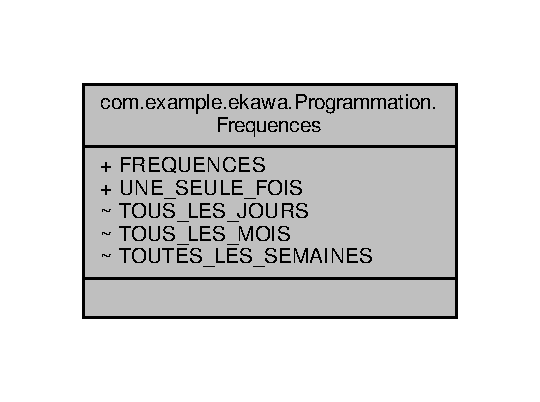
\includegraphics[width=259pt]{classcom_1_1example_1_1ekawa_1_1_programmation_1_1_frequences__coll__graph}
\end{center}
\end{figure}
\subsubsection*{Attributs publics statiques}
\begin{DoxyCompactItemize}
\item 
static final String \mbox{[}$\,$\mbox{]} \hyperlink{classcom_1_1example_1_1ekawa_1_1_programmation_1_1_frequences_afdc0109428ca2cc827cff55b8427cd50}{F\+R\+E\+Q\+U\+E\+N\+C\+ES}
\item 
static final int \hyperlink{classcom_1_1example_1_1ekawa_1_1_programmation_1_1_frequences_a92b76aab3e8479b140194ab329a0f3de}{U\+N\+E\+\_\+\+S\+E\+U\+L\+E\+\_\+\+F\+O\+IS} = 0
\end{DoxyCompactItemize}


\subsubsection{Description détaillée}


Définition à la ligne \hyperlink{_programmation_8java_source_l00059}{59} du fichier \hyperlink{_programmation_8java_source}{Programmation.\+java}.



\subsubsection{Documentation des données membres}
\mbox{\Hypertarget{classcom_1_1example_1_1ekawa_1_1_programmation_1_1_frequences_afdc0109428ca2cc827cff55b8427cd50}\label{classcom_1_1example_1_1ekawa_1_1_programmation_1_1_frequences_afdc0109428ca2cc827cff55b8427cd50}} 
\index{com\+::example\+::ekawa\+::\+Programmation\+::\+Frequences@{com\+::example\+::ekawa\+::\+Programmation\+::\+Frequences}!F\+R\+E\+Q\+U\+E\+N\+C\+ES@{F\+R\+E\+Q\+U\+E\+N\+C\+ES}}
\index{F\+R\+E\+Q\+U\+E\+N\+C\+ES@{F\+R\+E\+Q\+U\+E\+N\+C\+ES}!com\+::example\+::ekawa\+::\+Programmation\+::\+Frequences@{com\+::example\+::ekawa\+::\+Programmation\+::\+Frequences}}
\paragraph{\texorpdfstring{F\+R\+E\+Q\+U\+E\+N\+C\+ES}{FREQUENCES}}
{\footnotesize\ttfamily final String \mbox{[}$\,$\mbox{]} com.\+example.\+ekawa.\+Programmation.\+Frequences.\+F\+R\+E\+Q\+U\+E\+N\+C\+ES\hspace{0.3cm}{\ttfamily [static]}}

{\bfseries Valeur initiale \+:}
\begin{DoxyCode}
=
        \{
            \textcolor{stringliteral}{"Une seule fois"},
            \textcolor{stringliteral}{"Tous les jours"},
            \textcolor{stringliteral}{"Toutes les semaines"},
            \textcolor{stringliteral}{"Tous les mois"}
        \}
\end{DoxyCode}


Définition à la ligne \hyperlink{_programmation_8java_source_l00067}{67} du fichier \hyperlink{_programmation_8java_source}{Programmation.\+java}.



Référencé par \hyperlink{_ihm_8java_source_l00190}{com.\+example.\+ekawa.\+Ihm.\+Adaptateur\+Programmer.\+Adaptateur\+Programmer()}, et \hyperlink{_ihm_8java_source_l00727}{com.\+example.\+ekawa.\+Ihm.\+initialiser\+Fenetre\+Programmer()}.

\mbox{\Hypertarget{classcom_1_1example_1_1ekawa_1_1_programmation_1_1_frequences_a92b76aab3e8479b140194ab329a0f3de}\label{classcom_1_1example_1_1ekawa_1_1_programmation_1_1_frequences_a92b76aab3e8479b140194ab329a0f3de}} 
\index{com\+::example\+::ekawa\+::\+Programmation\+::\+Frequences@{com\+::example\+::ekawa\+::\+Programmation\+::\+Frequences}!U\+N\+E\+\_\+\+S\+E\+U\+L\+E\+\_\+\+F\+O\+IS@{U\+N\+E\+\_\+\+S\+E\+U\+L\+E\+\_\+\+F\+O\+IS}}
\index{U\+N\+E\+\_\+\+S\+E\+U\+L\+E\+\_\+\+F\+O\+IS@{U\+N\+E\+\_\+\+S\+E\+U\+L\+E\+\_\+\+F\+O\+IS}!com\+::example\+::ekawa\+::\+Programmation\+::\+Frequences@{com\+::example\+::ekawa\+::\+Programmation\+::\+Frequences}}
\paragraph{\texorpdfstring{U\+N\+E\+\_\+\+S\+E\+U\+L\+E\+\_\+\+F\+O\+IS}{UNE\_SEULE\_FOIS}}
{\footnotesize\ttfamily final int com.\+example.\+ekawa.\+Programmation.\+Frequences.\+U\+N\+E\+\_\+\+S\+E\+U\+L\+E\+\_\+\+F\+O\+IS = 0\hspace{0.3cm}{\ttfamily [static]}}



Définition à la ligne \hyperlink{_programmation_8java_source_l00062}{62} du fichier \hyperlink{_programmation_8java_source}{Programmation.\+java}.



Référencé par \hyperlink{_ihm_8java_source_l00938}{com.\+example.\+ekawa.\+Ihm.\+actualiser\+Page\+Programmer()}.



La documentation de cette classe a été générée à partir du fichier suivant \+:\begin{DoxyCompactItemize}
\item 
\hyperlink{_programmation_8java}{Programmation.\+java}\end{DoxyCompactItemize}

\hypertarget{classcom_1_1example_1_1ekawa_1_1_ihm}{}\subsection{Référence de la classe com.\+example.\+ekawa.\+Ihm}
\label{classcom_1_1example_1_1ekawa_1_1_ihm}\index{com.\+example.\+ekawa.\+Ihm@{com.\+example.\+ekawa.\+Ihm}}


Déclaration de l\textquotesingle{}activité principale de l\textquotesingle{}application Ekawa.  




Graphe de collaboration de com.\+example.\+ekawa.\+Ihm\+:\nopagebreak
\begin{figure}[H]
\begin{center}
\leavevmode
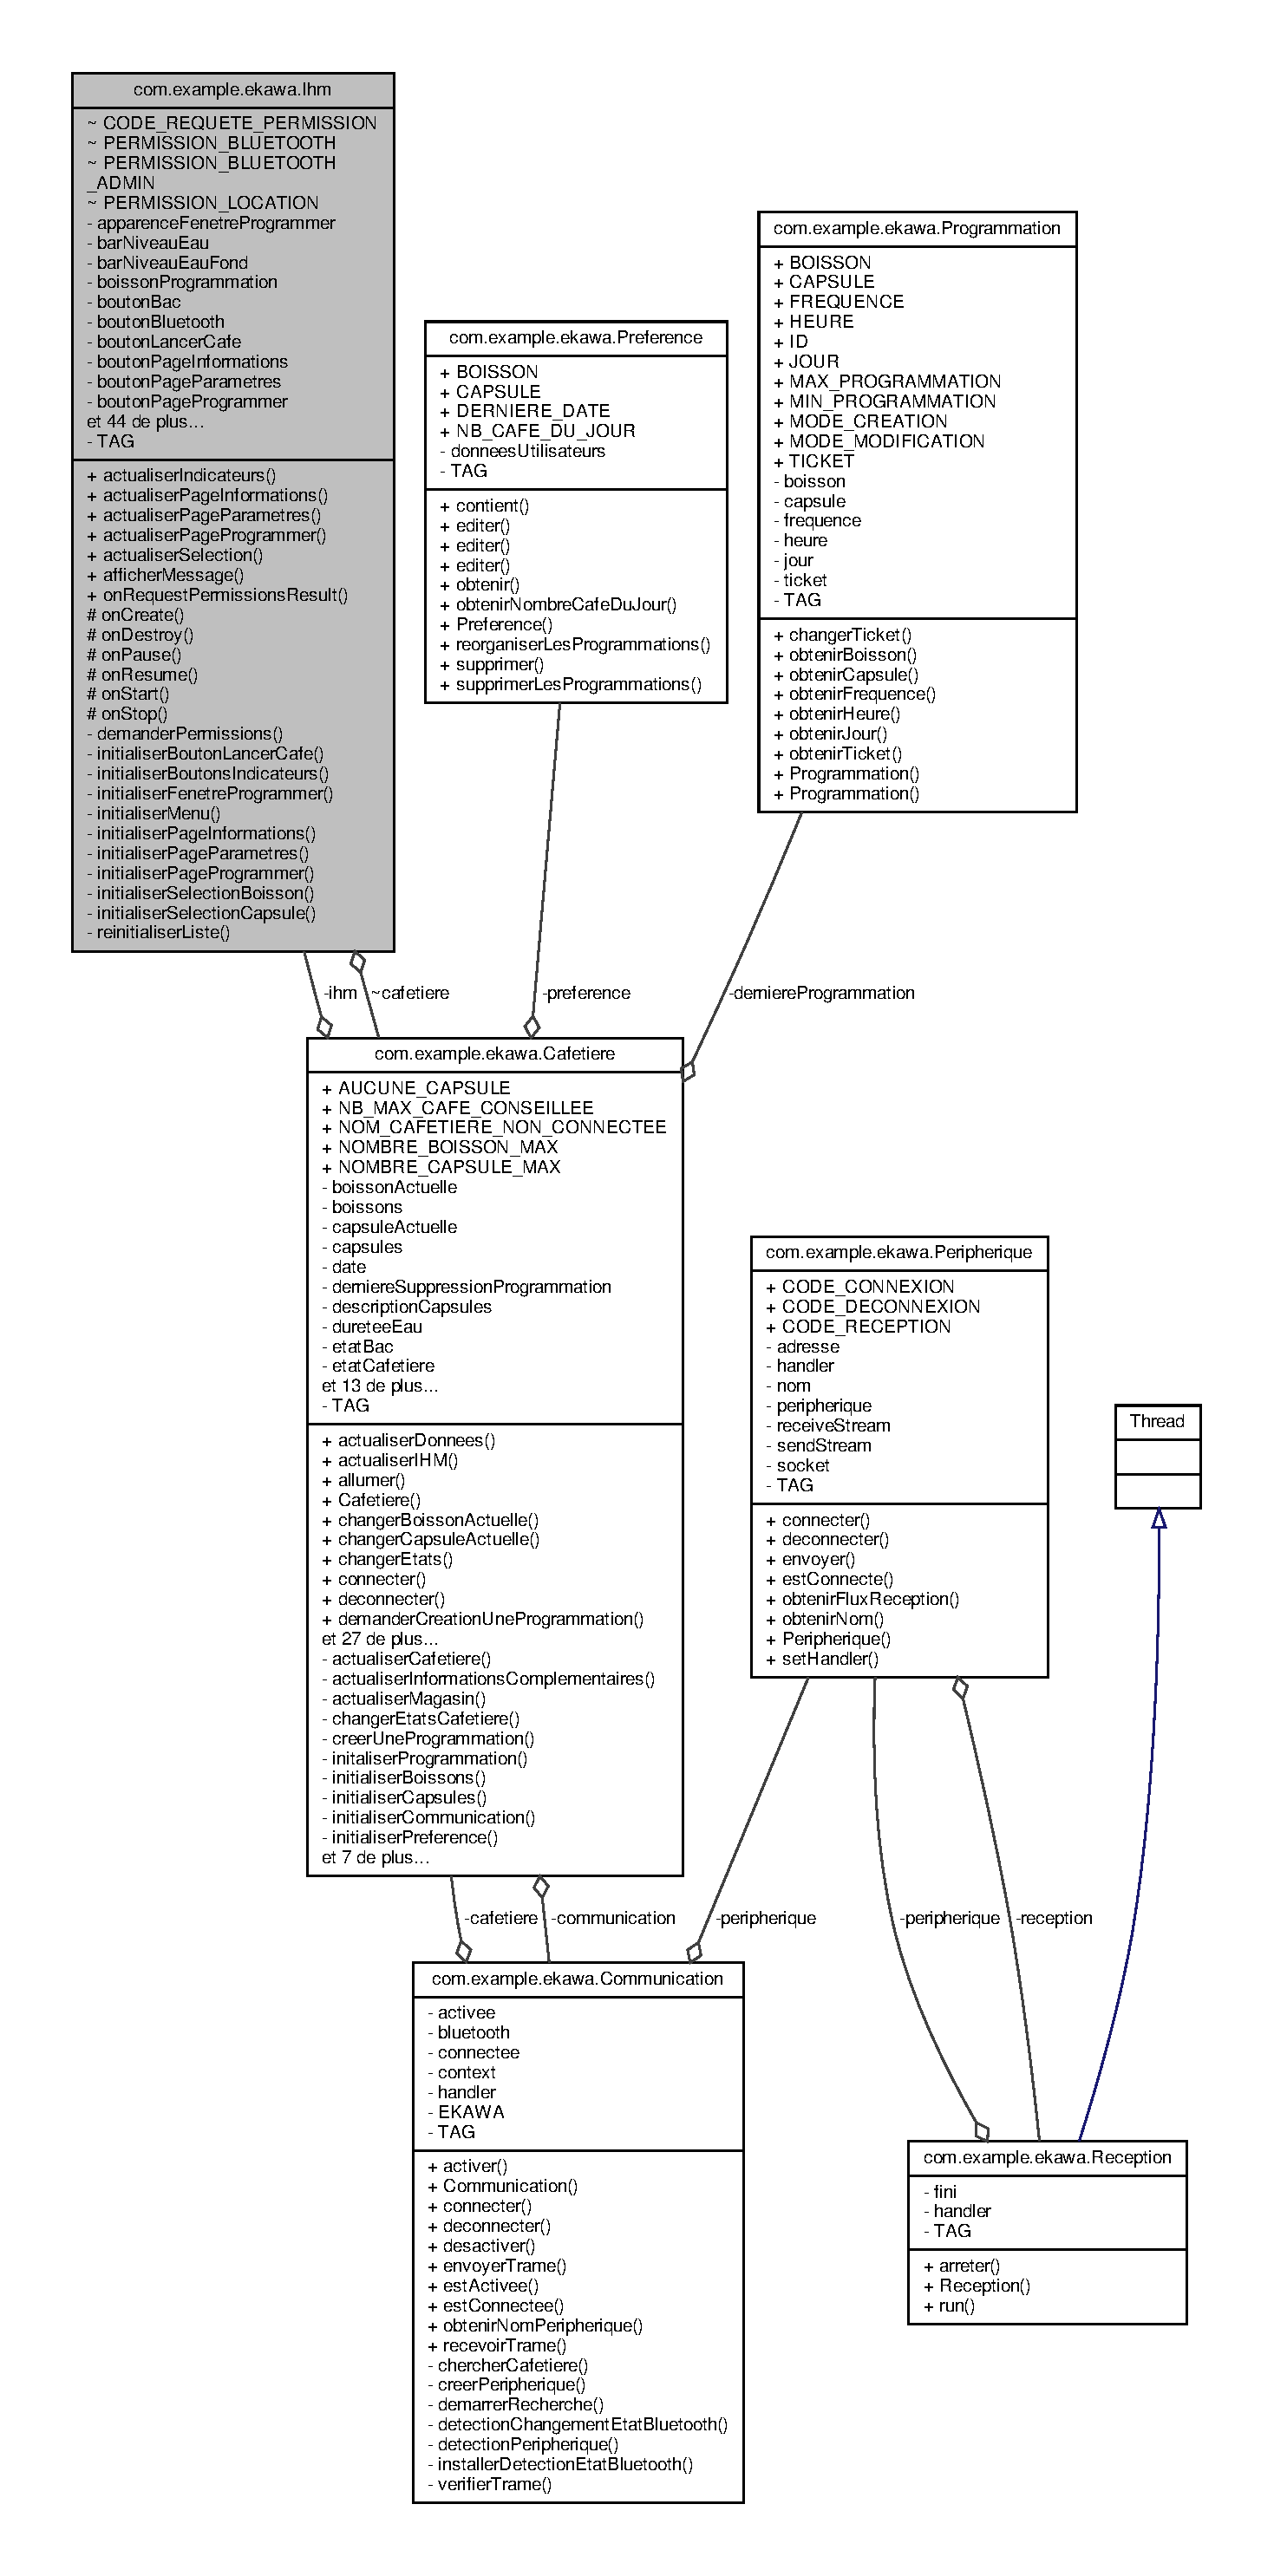
\includegraphics[height=550pt]{classcom_1_1example_1_1ekawa_1_1_ihm__coll__graph}
\end{center}
\end{figure}
\subsubsection*{Classes}
\begin{DoxyCompactItemize}
\item 
class \hyperlink{classcom_1_1example_1_1ekawa_1_1_ihm_1_1_adaptateur_programmer}{Adaptateur\+Programmer}
\item 
class \hyperlink{classcom_1_1example_1_1ekawa_1_1_ihm_1_1_adaptateur_selection}{Adaptateur\+Selection}
\end{DoxyCompactItemize}
\subsubsection*{Fonctions membres publiques}
\begin{DoxyCompactItemize}
\item 
void \hyperlink{classcom_1_1example_1_1ekawa_1_1_ihm_a2c3740dd5be20b3111b36649514fd41e}{actualiser\+Indicateurs} ()
\begin{DoxyCompactList}\small\item\em Méthode qui permet de mettre à jour les indicateurs (bluetooth, tasse, bac, eau) \end{DoxyCompactList}\item 
void \hyperlink{classcom_1_1example_1_1ekawa_1_1_ihm_a2422719a8e893b23e95f80b5899adb76}{actualiser\+Page\+Informations} ()
\begin{DoxyCompactList}\small\item\em Méthode qui permet d\textquotesingle{}actualiser la page \char`\"{}\+Informations\char`\"{}. \end{DoxyCompactList}\item 
void \hyperlink{classcom_1_1example_1_1ekawa_1_1_ihm_a7eca80c1cbf9a0f0f5c82dd79d32f4f4}{actualiser\+Page\+Parametres} ()
\begin{DoxyCompactList}\small\item\em Méthode qui permet d\textquotesingle{}actualiser la page \char`\"{}\+Parametres\char`\"{}. \end{DoxyCompactList}\item 
void \hyperlink{classcom_1_1example_1_1ekawa_1_1_ihm_adbeeac61b5a53c52d21da490659de983}{actualiser\+Page\+Programmer} ()
\begin{DoxyCompactList}\small\item\em Méthode qui permet d\textquotesingle{}actualiser la page \char`\"{}\+Programmer\char`\"{}. \end{DoxyCompactList}\item 
void \hyperlink{classcom_1_1example_1_1ekawa_1_1_ihm_a2d7fd2fe397785acc2b9a32e65cfd52f}{actualiser\+Selection} ()
\begin{DoxyCompactList}\small\item\em Méthode qui permet de mettre à jour la liste des selections des capsules. \end{DoxyCompactList}\item 
void \hyperlink{classcom_1_1example_1_1ekawa_1_1_ihm_ab1ca33ad18d42540299e3a58a82f4d9a}{afficher\+Message} (String texte)
\begin{DoxyCompactList}\small\item\em Méthode qui permet d\textquotesingle{}afficher des messages. \end{DoxyCompactList}\item 
void \hyperlink{classcom_1_1example_1_1ekawa_1_1_ihm_a708f7d3adb02a942cb67a5d6ec42b64f}{on\+Request\+Permissions\+Result} (int request\+Code, String permissions\mbox{[}$\,$\mbox{]}, int\mbox{[}$\,$\mbox{]} grant\+Results)
\begin{DoxyCompactList}\small\item\em Méthode qui permet de gérer la réponse à la demande de permission location. \end{DoxyCompactList}\end{DoxyCompactItemize}
\subsubsection*{Fonctions membres protégées}
\begin{DoxyCompactItemize}
\item 
void \hyperlink{classcom_1_1example_1_1ekawa_1_1_ihm_af37a1d1d731eaed5e9cc19d23475ede3}{on\+Create} (Bundle saved\+Instance\+State)
\begin{DoxyCompactList}\small\item\em Méthode appelée à la création de l\textquotesingle{}activité \end{DoxyCompactList}\item 
void \hyperlink{classcom_1_1example_1_1ekawa_1_1_ihm_a5ae27969ec39afede5d0cd36b469f145}{on\+Destroy} ()
\begin{DoxyCompactList}\small\item\em Méthode appelée à la destruction de l\textquotesingle{}application (après \hyperlink{classcom_1_1example_1_1ekawa_1_1_ihm_adc7bc6671d8cd5018724bcbf4fbc0d75}{on\+Stop()} et détruite par le système Android) \end{DoxyCompactList}\item 
void \hyperlink{classcom_1_1example_1_1ekawa_1_1_ihm_a4cf2ee6861e571d2634a4dd2492e9be9}{on\+Pause} ()
\begin{DoxyCompactList}\small\item\em Méthode appelée après qu\textquotesingle{}une boîte de dialogue s\textquotesingle{}est affichée (on reprend sur un \hyperlink{classcom_1_1example_1_1ekawa_1_1_ihm_aec9b38c2990ae4bdee8df0b49253120f}{on\+Resume()}) ou avant \hyperlink{classcom_1_1example_1_1ekawa_1_1_ihm_adc7bc6671d8cd5018724bcbf4fbc0d75}{on\+Stop()} (activité plus visible) \end{DoxyCompactList}\item 
void \hyperlink{classcom_1_1example_1_1ekawa_1_1_ihm_aec9b38c2990ae4bdee8df0b49253120f}{on\+Resume} ()
\begin{DoxyCompactList}\small\item\em Méthode appelée après \hyperlink{classcom_1_1example_1_1ekawa_1_1_ihm_a5cf91e6625760cbdca208988a08e86f6}{on\+Start()} ou après \hyperlink{classcom_1_1example_1_1ekawa_1_1_ihm_a4cf2ee6861e571d2634a4dd2492e9be9}{on\+Pause()} \end{DoxyCompactList}\item 
void \hyperlink{classcom_1_1example_1_1ekawa_1_1_ihm_a5cf91e6625760cbdca208988a08e86f6}{on\+Start} ()
\begin{DoxyCompactList}\small\item\em Méthode appelée au démarrage après le \hyperlink{classcom_1_1example_1_1ekawa_1_1_ihm_af37a1d1d731eaed5e9cc19d23475ede3}{on\+Create()} ou un restart après un \hyperlink{classcom_1_1example_1_1ekawa_1_1_ihm_adc7bc6671d8cd5018724bcbf4fbc0d75}{on\+Stop()} \end{DoxyCompactList}\item 
void \hyperlink{classcom_1_1example_1_1ekawa_1_1_ihm_adc7bc6671d8cd5018724bcbf4fbc0d75}{on\+Stop} ()
\begin{DoxyCompactList}\small\item\em Méthode appelée lorsque l\textquotesingle{}activité n\textquotesingle{}est plus visible. \end{DoxyCompactList}\end{DoxyCompactItemize}
\subsubsection*{Fonctions membres privées}
\begin{DoxyCompactItemize}
\item 
void \hyperlink{classcom_1_1example_1_1ekawa_1_1_ihm_a30e0dc3bf57b1abc608cb8b932527566}{demander\+Permissions} ()
\begin{DoxyCompactList}\small\item\em Méthode qui permet de demander le droit de permission location. \end{DoxyCompactList}\item 
void \hyperlink{classcom_1_1example_1_1ekawa_1_1_ihm_a6616a5f240867f43c8e56f2b432e43be}{initialiser\+Bouton\+Lancer\+Cafe} ()
\begin{DoxyCompactList}\small\item\em Méthode qui permet d\textquotesingle{}initialiser le bouton principal de l\textquotesingle{}application (pour lancer le café) \end{DoxyCompactList}\item 
void \hyperlink{classcom_1_1example_1_1ekawa_1_1_ihm_ae38db41c355bc415b46f21f9d608d4b9}{initialiser\+Boutons\+Indicateurs} ()
\begin{DoxyCompactList}\small\item\em Méthode qui permet d\textquotesingle{}initialiser les indicateurs (bluetooth, tasse, bac, eau) \end{DoxyCompactList}\item 
void \hyperlink{classcom_1_1example_1_1ekawa_1_1_ihm_a08b1da8fdc68effff9a6da918e14d12d}{initialiser\+Fenetre\+Programmer} ()
\begin{DoxyCompactList}\small\item\em Méthode qui permet d\textquotesingle{}initialiser la fenetre volante \char`\"{}\+Programmer\char`\"{}. \end{DoxyCompactList}\item 
void \hyperlink{classcom_1_1example_1_1ekawa_1_1_ihm_a60968cecc69df879805b531a5f2ae19c}{initialiser\+Menu} ()
\begin{DoxyCompactList}\small\item\em Méthode qui permet d\textquotesingle{}initialiser le menu (page \char`\"{}informations\char`\"{}, page \char`\"{}programmer\char`\"{}, page \char`\"{}paramètres\char`\"{}) \end{DoxyCompactList}\item 
void \hyperlink{classcom_1_1example_1_1ekawa_1_1_ihm_ad431346f0a437b4f23697208c5048a02}{initialiser\+Page\+Informations} ()
\begin{DoxyCompactList}\small\item\em Méthode qui permet d\textquotesingle{}initialiser la page \char`\"{}\+Informations\char`\"{}. \end{DoxyCompactList}\item 
void \hyperlink{classcom_1_1example_1_1ekawa_1_1_ihm_af18a3c8df11503003c92e8e5de89b7c3}{initialiser\+Page\+Parametres} ()
\begin{DoxyCompactList}\small\item\em Méthode qui permet d\textquotesingle{}initialiser la page \char`\"{}\+Parametres\char`\"{}. \end{DoxyCompactList}\item 
void \hyperlink{classcom_1_1example_1_1ekawa_1_1_ihm_aa5ef2c0c4b4cefb518ec4f3e05b098aa}{initialiser\+Page\+Programmer} ()
\begin{DoxyCompactList}\small\item\em Méthode qui permet d\textquotesingle{}initialiser la page \char`\"{}\+Programmer\char`\"{}. \end{DoxyCompactList}\item 
void \hyperlink{classcom_1_1example_1_1ekawa_1_1_ihm_a0a4086cea2ee9d6d18c957513706cbce}{initialiser\+Selection\+Boisson} ()
\begin{DoxyCompactList}\small\item\em Méthode qui permet d\textquotesingle{}initialiser la liste de selection des boissons. \end{DoxyCompactList}\item 
void \hyperlink{classcom_1_1example_1_1ekawa_1_1_ihm_a32a1b0d802eef67b6c838d8839de7bdb}{initialiser\+Selection\+Capsule} ()
\begin{DoxyCompactList}\small\item\em Méthode qui permet d\textquotesingle{}initialiser la liste de selection des capsules. \end{DoxyCompactList}\item 
void \hyperlink{classcom_1_1example_1_1ekawa_1_1_ihm_a4c6ea5a7de9f8fc5c820fa4c8ce14838}{reinitialiser\+Liste} (List\+View liste)
\begin{DoxyCompactList}\small\item\em Méthode qui permet de reinitialiser une liste. \end{DoxyCompactList}\end{DoxyCompactItemize}
\subsubsection*{Attributs privés}
\begin{DoxyCompactItemize}
\item 
View \hyperlink{classcom_1_1example_1_1ekawa_1_1_ihm_aa8beb9a05b4f2c2030b9829642f87d3f}{apparence\+Fenetre\+Programmer}
\item 
Progress\+Bar \hyperlink{classcom_1_1example_1_1ekawa_1_1_ihm_a9023d37b98385b21d2b5dd6910c13020}{bar\+Niveau\+Eau}
\item 
Progress\+Bar \hyperlink{classcom_1_1example_1_1ekawa_1_1_ihm_a104a80153a74a9cbcbd757c24ce84a36}{bar\+Niveau\+Eau\+Fond}
\item 
int \hyperlink{classcom_1_1example_1_1ekawa_1_1_ihm_a6ad8136ec35fff9e96476c4f35726fea}{boisson\+Programmation} = 0
\item 
Image\+Button \hyperlink{classcom_1_1example_1_1ekawa_1_1_ihm_a6c4ca9f4166d4ceee1bee82b4f7508a4}{bouton\+Bac}
\item 
Image\+Button \hyperlink{classcom_1_1example_1_1ekawa_1_1_ihm_a0c2ec4e1fa0085520fa9db31ee4284fc}{bouton\+Bluetooth}
\item 
Frame\+Layout \hyperlink{classcom_1_1example_1_1ekawa_1_1_ihm_af64465b03533ddddfaac1a55b0f14012}{bouton\+Lancer\+Cafe}
\item 
Linear\+Layout \hyperlink{classcom_1_1example_1_1ekawa_1_1_ihm_a93dd279f2c6fa8d4e22ce298b1c4ab16}{bouton\+Page\+Informations}
\item 
Linear\+Layout \hyperlink{classcom_1_1example_1_1ekawa_1_1_ihm_a11fe63d247e6b4966aac0086c06bd495}{bouton\+Page\+Parametres}
\item 
Linear\+Layout \hyperlink{classcom_1_1example_1_1ekawa_1_1_ihm_a15ad5787c0800a7a2e2f00964787255f}{bouton\+Page\+Programmer}
\item 
Button \hyperlink{classcom_1_1example_1_1ekawa_1_1_ihm_aa910a5ff04c7003b0035f89572310652}{bouton\+Reinitialiser\+Informations}
\item 
Frame\+Layout \hyperlink{classcom_1_1example_1_1ekawa_1_1_ihm_a5aec848e98e7bd8b933b87e390de809e}{bouton\+Selection\+Boisson}
\item 
Frame\+Layout \hyperlink{classcom_1_1example_1_1ekawa_1_1_ihm_a866bc916203a767c5f9def913b59175d}{bouton\+Selection\+Capsule}
\item 
Image\+Button \hyperlink{classcom_1_1example_1_1ekawa_1_1_ihm_a32e7322f35858a93cdfb75e06f788842}{bouton\+Tasse}
\item 
int \hyperlink{classcom_1_1example_1_1ekawa_1_1_ihm_a2ddf5b95e2a3fbb3a15d160ba266295a}{capsule\+Programmation} = 0
\item 
Alert\+Dialog \hyperlink{classcom_1_1example_1_1ekawa_1_1_ihm_a369f219339f23afe8a6d1d93bf6611ca}{fenetre\+Informations}
\item 
Alert\+Dialog \hyperlink{classcom_1_1example_1_1ekawa_1_1_ihm_addac9c5f93086d06e5131cd42f3be941}{fenetre\+Programmer}
\item 
Time\+Picker \hyperlink{classcom_1_1example_1_1ekawa_1_1_ihm_ac6f46062030a20efac18673970d37547}{heure\+Programmer}
\item 
Integer \mbox{[}$\,$\mbox{]} \hyperlink{classcom_1_1example_1_1ekawa_1_1_ihm_aab3ed36de15018dd29af2df4b3e150e4}{identifiants\+Images\+Boisson}
\item 
Integer \mbox{[}$\,$\mbox{]} \hyperlink{classcom_1_1example_1_1ekawa_1_1_ihm_af35b42764d9f7b10c8bc0e210c3ba76d}{identifiants\+Images\+Capsules}
\item 
Image\+View \hyperlink{classcom_1_1example_1_1ekawa_1_1_ihm_a2d83809a52b5f9a97f7817ae183c456d}{image\+Boisson\+Actuelle}
\item 
Image\+View \hyperlink{classcom_1_1example_1_1ekawa_1_1_ihm_a82418c4769be80ea67628e2ae8e85ee4}{image\+Capsule\+Actuelle}
\item 
List\+View \hyperlink{classcom_1_1example_1_1ekawa_1_1_ihm_a8badf9f0485d205f8a379e54b01deab7}{liste\+Boisson\+Programmer}
\item 
List\+View \hyperlink{classcom_1_1example_1_1ekawa_1_1_ihm_a955e0c1674ee1ddfbf05f3ef6a081d67}{liste\+Capsule}
\item 
List\+View \hyperlink{classcom_1_1example_1_1ekawa_1_1_ihm_adfeb58df0ce9fa2088a7a708a54ffe07}{liste\+Capsule\+Programmer}
\item 
List\+View \hyperlink{classcom_1_1example_1_1ekawa_1_1_ihm_a4fd152e506a6b1130477795d8c2d2a83}{liste\+Programmer}
\item 
List\+View \hyperlink{classcom_1_1example_1_1ekawa_1_1_ihm_a6f81eeec5d65c16e33b7ac67b4e771cb}{liste\+Selection\+Boisson}
\item 
List\+View \hyperlink{classcom_1_1example_1_1ekawa_1_1_ihm_a0842447d70bca2098431fa532c1c94e8}{liste\+Selection\+Capsule}
\item 
boolean \hyperlink{classcom_1_1example_1_1ekawa_1_1_ihm_acc8db4ba4fa39c343412d6ff57c2acbd}{mode\+Programmer}
\item 
String \mbox{[}$\,$\mbox{]} \hyperlink{classcom_1_1example_1_1ekawa_1_1_ihm_abafa700d1d1f943bd3e9678f698ed33a}{noms\+Boisson}
\item 
String \mbox{[}$\,$\mbox{]} \hyperlink{classcom_1_1example_1_1ekawa_1_1_ihm_a9d61b7bfd998d449bb405dcf5e6e4e89}{noms\+Capsules}
\item 
Linear\+Layout \hyperlink{classcom_1_1example_1_1ekawa_1_1_ihm_a554ab8cbe600e837516ec78e62312fea}{page\+Informations}
\item 
Linear\+Layout \hyperlink{classcom_1_1example_1_1ekawa_1_1_ihm_a12537211f4d695c3dc62713da00ffa35}{page\+Parametres}
\item 
Linear\+Layout \hyperlink{classcom_1_1example_1_1ekawa_1_1_ihm_a9a3747e82c5917a681a8d8a726cd5fa8}{page\+Programmer}
\item 
Alert\+Dialog.\+Builder \hyperlink{classcom_1_1example_1_1ekawa_1_1_ihm_a610b25d0bf8b26fbf1ed24345acef189}{parametres\+Fenetre\+Informations}
\item 
Alert\+Dialog.\+Builder \hyperlink{classcom_1_1example_1_1ekawa_1_1_ihm_a6eb2afb2fe8da7f3a749089c84934145}{parametres\+Fenetre\+Programmer}
\item 
int \hyperlink{classcom_1_1example_1_1ekawa_1_1_ihm_ada29cde0c67d8614d47b27ed04c337e9}{position\+Programmer}
\item 
Spinner \hyperlink{classcom_1_1example_1_1ekawa_1_1_ihm_ab266576a3855dbd6e36e346ddb27247a}{spinner\+Frequence\+Programmer}
\item 
Spinner \hyperlink{classcom_1_1example_1_1ekawa_1_1_ihm_a49e6261929f259b2fcc81bf13d21ad7f}{spinner\+Jour\+Programmer}
\item 
Text\+View \hyperlink{classcom_1_1example_1_1ekawa_1_1_ihm_a6655fee013d48228f2c7981f1cd8f74e}{texte\+Boisson\+Actuelle}
\item 
Text\+View \hyperlink{classcom_1_1example_1_1ekawa_1_1_ihm_a3a9c8a185607e09fed0df62e46925786}{texte\+Capsule\+Actuelle}
\item 
Text\+View \hyperlink{classcom_1_1example_1_1ekawa_1_1_ihm_ac19dc1f761f988fcd51bbdb6f67a4009}{texte\+Duretee\+Eau}
\item 
Text\+View \hyperlink{classcom_1_1example_1_1ekawa_1_1_ihm_a96074c1992a3a44734b3c82e5cdf073b}{texte\+Nb\+Bac}
\item 
Text\+View \hyperlink{classcom_1_1example_1_1ekawa_1_1_ihm_a30418331964030ba9c2cb5f4e7b34b2c}{texte\+Nb\+Cafe}
\item 
Text\+View \hyperlink{classcom_1_1example_1_1ekawa_1_1_ihm_a06f0f159882f0c5c3e3cca7f698489c9}{texte\+Nb\+Cafe\+Jour}
\item 
Text\+View \hyperlink{classcom_1_1example_1_1ekawa_1_1_ihm_a6abf08d241bab230727c22069aa7913c}{texte\+Nb\+Eau}
\item 
Text\+View \hyperlink{classcom_1_1example_1_1ekawa_1_1_ihm_aa20f5ea009dec0e50b6df5aaffbb690c}{texte\+Niveau\+Eau}
\item 
Text\+View \hyperlink{classcom_1_1example_1_1ekawa_1_1_ihm_abc84321aabf4b59d9e452afdb878357f}{texte\+Nom\+Cafetiere}
\item 
Text\+View \hyperlink{classcom_1_1example_1_1ekawa_1_1_ihm_af66cb31129c00413279e8254a6599143}{texte\+Qualitee\+Eau}
\item 
boolean \hyperlink{classcom_1_1example_1_1ekawa_1_1_ihm_a874a157d2a92d1a386a06512f36182ff}{visibilite\+Liste\+Selection\+Boisson} = false
\item 
boolean \hyperlink{classcom_1_1example_1_1ekawa_1_1_ihm_aa6b9cda83ef1aba8816fd43797fb7ab2}{visibilite\+Liste\+Selection\+Capsule} = false
\item 
boolean \hyperlink{classcom_1_1example_1_1ekawa_1_1_ihm_a3a1aee8b3e12447c5a73aa16de64b1f0}{visibilite\+Page\+Informations} = false
\item 
boolean \hyperlink{classcom_1_1example_1_1ekawa_1_1_ihm_abc6f7d562f994f120a9034a9e11b72d0}{visibilite\+Page\+Parametres} = false
\item 
boolean \hyperlink{classcom_1_1example_1_1ekawa_1_1_ihm_a1db719bfa9b48f6c1f64259e37703963}{visibilite\+Page\+Programmer} = false
\end{DoxyCompactItemize}
\subsubsection*{Attributs privés statiques}
\begin{DoxyCompactItemize}
\item 
static final String \hyperlink{classcom_1_1example_1_1ekawa_1_1_ihm_a95cd92c2acaf9f8982302da08d94f9aa}{T\+AG} = \char`\"{}\+\_\+\+Ihm\char`\"{}
\begin{DoxyCompactList}\small\item\em T\+AG pour les logs. \end{DoxyCompactList}\end{DoxyCompactItemize}


\subsubsection{Description détaillée}
Déclaration de l\textquotesingle{}activité principale de l\textquotesingle{}application Ekawa. 

Définition à la ligne \hyperlink{_ihm_8java_source_l00054}{54} du fichier \hyperlink{_ihm_8java_source}{Ihm.\+java}.



\subsubsection{Documentation des fonctions membres}
\mbox{\Hypertarget{classcom_1_1example_1_1ekawa_1_1_ihm_a2c3740dd5be20b3111b36649514fd41e}\label{classcom_1_1example_1_1ekawa_1_1_ihm_a2c3740dd5be20b3111b36649514fd41e}} 
\index{com\+::example\+::ekawa\+::\+Ihm@{com\+::example\+::ekawa\+::\+Ihm}!actualiser\+Indicateurs@{actualiser\+Indicateurs}}
\index{actualiser\+Indicateurs@{actualiser\+Indicateurs}!com\+::example\+::ekawa\+::\+Ihm@{com\+::example\+::ekawa\+::\+Ihm}}
\paragraph{\texorpdfstring{actualiser\+Indicateurs()}{actualiserIndicateurs()}}
{\footnotesize\ttfamily void com.\+example.\+ekawa.\+Ihm.\+actualiser\+Indicateurs (\begin{DoxyParamCaption}{ }\end{DoxyParamCaption})}



Méthode qui permet de mettre à jour les indicateurs (bluetooth, tasse, bac, eau) 



Définition à la ligne \hyperlink{_ihm_8java_source_l00855}{855} du fichier \hyperlink{_ihm_8java_source}{Ihm.\+java}.



Références \hyperlink{_cafetiere_8java_source_l00028}{com.\+example.\+ekawa.\+Cafetiere.\+A\+U\+C\+U\+N\+E\+\_\+\+C\+A\+P\+S\+U\+LE}, \hyperlink{_cafetiere_8java_source_l00235}{com.\+example.\+ekawa.\+Cafetiere.\+informer\+Capsule\+Actuelle()}, \hyperlink{_cafetiere_8java_source_l00275}{com.\+example.\+ekawa.\+Cafetiere.\+informer\+Connexion\+Bluetooth()}, \hyperlink{_cafetiere_8java_source_l00295}{com.\+example.\+ekawa.\+Cafetiere.\+informer\+Etat\+Bac()}, \hyperlink{_cafetiere_8java_source_l00265}{com.\+example.\+ekawa.\+Cafetiere.\+informer\+Etat\+Bluetooth()}, \hyperlink{_cafetiere_8java_source_l00255}{com.\+example.\+ekawa.\+Cafetiere.\+informer\+Etat\+Cafetiere()}, \hyperlink{_cafetiere_8java_source_l00285}{com.\+example.\+ekawa.\+Cafetiere.\+informer\+Etat\+Tasse()}, et \hyperlink{_cafetiere_8java_source_l00305}{com.\+example.\+ekawa.\+Cafetiere.\+informer\+Niveau\+Eau()}.



Référencé par \hyperlink{_cafetiere_8java_source_l00543}{com.\+example.\+ekawa.\+Cafetiere.\+actualiser\+Cafetiere()}, \hyperlink{_cafetiere_8java_source_l00674}{com.\+example.\+ekawa.\+Cafetiere.\+actualiser\+I\+H\+M()}, \hyperlink{_cafetiere_8java_source_l00212}{com.\+example.\+ekawa.\+Cafetiere.\+changer\+Capsule\+Actuelle()}, \hyperlink{_cafetiere_8java_source_l00527}{com.\+example.\+ekawa.\+Cafetiere.\+lancer\+Preparation\+Cafe()}, \hyperlink{_ihm_8java_source_l00248}{com.\+example.\+ekawa.\+Ihm.\+on\+Create()}, \hyperlink{_ihm_8java_source_l00284}{com.\+example.\+ekawa.\+Ihm.\+on\+Resume()}, et \hyperlink{_cafetiere_8java_source_l00658}{com.\+example.\+ekawa.\+Cafetiere.\+remettre\+A\+Zero()}.


\begin{DoxyCode}
00856     \{
00857         Log.d(\hyperlink{classcom_1_1example_1_1ekawa_1_1_ihm_a95cd92c2acaf9f8982302da08d94f9aa}{TAG}, \textcolor{stringliteral}{"actualiserIndicateurs()"});
00858         \textcolor{keywordflow}{if} (cafetiere.\hyperlink{classcom_1_1example_1_1ekawa_1_1_cafetiere_aeff88ad385713a7897074dcdb76077a5}{informerEtatBluetooth}() && cafetiere.
      \hyperlink{classcom_1_1example_1_1ekawa_1_1_cafetiere_a97d9ca4701a961fe8865ecfa1d5bf64a}{informerConnexionBluetooth}())
00859             \hyperlink{classcom_1_1example_1_1ekawa_1_1_ihm_a0c2ec4e1fa0085520fa9db31ee4284fc}{boutonBluetooth}.setBackgroundResource(R.drawable.style\_bouton\_valide);
00860         \textcolor{keywordflow}{else} \textcolor{keywordflow}{if} (cafetiere.\hyperlink{classcom_1_1example_1_1ekawa_1_1_cafetiere_aeff88ad385713a7897074dcdb76077a5}{informerEtatBluetooth}() && !cafetiere.
      \hyperlink{classcom_1_1example_1_1ekawa_1_1_cafetiere_a97d9ca4701a961fe8865ecfa1d5bf64a}{informerConnexionBluetooth}())
00861             \hyperlink{classcom_1_1example_1_1ekawa_1_1_ihm_a0c2ec4e1fa0085520fa9db31ee4284fc}{boutonBluetooth}.setBackgroundResource(R.drawable.style\_bouton\_semi\_valide);
00862         \textcolor{keywordflow}{else}
00863             \hyperlink{classcom_1_1example_1_1ekawa_1_1_ihm_a0c2ec4e1fa0085520fa9db31ee4284fc}{boutonBluetooth}.setBackgroundResource(R.drawable.style\_bouton\_invalide);
00864 
00865         \textcolor{keywordflow}{if} (cafetiere.\hyperlink{classcom_1_1example_1_1ekawa_1_1_cafetiere_ae3c04cc0258cbe554eee5894655c379e}{informerEtatTasse}())
00866             \hyperlink{classcom_1_1example_1_1ekawa_1_1_ihm_a32e7322f35858a93cdfb75e06f788842}{boutonTasse}.setBackgroundResource(R.drawable.style\_bouton\_valide);
00867         \textcolor{keywordflow}{else}
00868             \hyperlink{classcom_1_1example_1_1ekawa_1_1_ihm_a32e7322f35858a93cdfb75e06f788842}{boutonTasse}.setBackgroundResource(R.drawable.style\_bouton\_invalide);
00869 
00870         \textcolor{keywordflow}{if} (cafetiere.\hyperlink{classcom_1_1example_1_1ekawa_1_1_cafetiere_a1e5aad72cec77a755c8b70eb1be5e6e5}{informerEtatBac}())
00871             \hyperlink{classcom_1_1example_1_1ekawa_1_1_ihm_a6c4ca9f4166d4ceee1bee82b4f7508a4}{boutonBac}.setBackgroundResource(R.drawable.style\_bouton\_valide);
00872         \textcolor{keywordflow}{else}
00873             \hyperlink{classcom_1_1example_1_1ekawa_1_1_ihm_a6c4ca9f4166d4ceee1bee82b4f7508a4}{boutonBac}.setBackgroundResource(R.drawable.style\_bouton\_invalide);
00874 
00875         \textcolor{keywordflow}{if} (cafetiere.\hyperlink{classcom_1_1example_1_1ekawa_1_1_cafetiere_aeff88ad385713a7897074dcdb76077a5}{informerEtatBluetooth}() && cafetiere.
      \hyperlink{classcom_1_1example_1_1ekawa_1_1_cafetiere_a97d9ca4701a961fe8865ecfa1d5bf64a}{informerConnexionBluetooth}() && cafetiere.
      \hyperlink{classcom_1_1example_1_1ekawa_1_1_cafetiere_a3251d1865f3a4113553e1743a971984d}{informerCapsuleActuelle}() != Cafetiere.AUCUNE\_CAPSULE && cafetiere.
      \hyperlink{classcom_1_1example_1_1ekawa_1_1_cafetiere_a4253a092cf9c84f7b97021e628d5bfb4}{informerEtatCafetiere}() && cafetiere.\hyperlink{classcom_1_1example_1_1ekawa_1_1_cafetiere_ae3c04cc0258cbe554eee5894655c379e}{informerEtatTasse}() && cafetiere
      .\hyperlink{classcom_1_1example_1_1ekawa_1_1_cafetiere_a1e5aad72cec77a755c8b70eb1be5e6e5}{informerEtatBac}() && cafetiere.\hyperlink{classcom_1_1example_1_1ekawa_1_1_cafetiere_ab8113e922056276f8097744991ca76b6}{informerNiveauEau}() != 0)
00876         \{
00877             \hyperlink{classcom_1_1example_1_1ekawa_1_1_ihm_af64465b03533ddddfaac1a55b0f14012}{boutonLancerCafe}.setBackgroundResource(R.drawable.style\_bouton\_valide);
00878         \}
00879         \textcolor{keywordflow}{else}
00880         \{
00881             \hyperlink{classcom_1_1example_1_1ekawa_1_1_ihm_af64465b03533ddddfaac1a55b0f14012}{boutonLancerCafe}.setBackgroundResource(R.drawable.style\_bouton\_invalide);
00882         \}
00883 
00884         \hyperlink{classcom_1_1example_1_1ekawa_1_1_ihm_a104a80153a74a9cbcbd757c24ce84a36}{barNiveauEauFond}.setProgress(cafetiere.\hyperlink{classcom_1_1example_1_1ekawa_1_1_cafetiere_ab8113e922056276f8097744991ca76b6}{informerNiveauEau}());
00885         \hyperlink{classcom_1_1example_1_1ekawa_1_1_ihm_a9023d37b98385b21d2b5dd6910c13020}{barNiveauEau}.setProgress(cafetiere.\hyperlink{classcom_1_1example_1_1ekawa_1_1_cafetiere_ab8113e922056276f8097744991ca76b6}{informerNiveauEau}());
00886         \hyperlink{classcom_1_1example_1_1ekawa_1_1_ihm_aa20f5ea009dec0e50b6df5aaffbb690c}{texteNiveauEau}.setText(cafetiere.\hyperlink{classcom_1_1example_1_1ekawa_1_1_cafetiere_ab8113e922056276f8097744991ca76b6}{informerNiveauEau}() + \textcolor{stringliteral}{"%"});
00887     \}
\end{DoxyCode}
\mbox{\Hypertarget{classcom_1_1example_1_1ekawa_1_1_ihm_a2422719a8e893b23e95f80b5899adb76}\label{classcom_1_1example_1_1ekawa_1_1_ihm_a2422719a8e893b23e95f80b5899adb76}} 
\index{com\+::example\+::ekawa\+::\+Ihm@{com\+::example\+::ekawa\+::\+Ihm}!actualiser\+Page\+Informations@{actualiser\+Page\+Informations}}
\index{actualiser\+Page\+Informations@{actualiser\+Page\+Informations}!com\+::example\+::ekawa\+::\+Ihm@{com\+::example\+::ekawa\+::\+Ihm}}
\paragraph{\texorpdfstring{actualiser\+Page\+Informations()}{actualiserPageInformations()}}
{\footnotesize\ttfamily void com.\+example.\+ekawa.\+Ihm.\+actualiser\+Page\+Informations (\begin{DoxyParamCaption}{ }\end{DoxyParamCaption})}



Méthode qui permet d\textquotesingle{}actualiser la page \char`\"{}\+Informations\char`\"{}. 



Définition à la ligne \hyperlink{_ihm_8java_source_l00919}{919} du fichier \hyperlink{_ihm_8java_source}{Ihm.\+java}.



Références \hyperlink{_cafetiere_8java_source_l00378}{com.\+example.\+ekawa.\+Cafetiere.\+informer\+Duretee\+Eau()}, \hyperlink{_cafetiere_8java_source_l00358}{com.\+example.\+ekawa.\+Cafetiere.\+informer\+Nombre\+Bac\+Vide()}, \hyperlink{_cafetiere_8java_source_l00326}{com.\+example.\+ekawa.\+Cafetiere.\+informer\+Nombre\+Cafe\+Du\+Jour()}, \hyperlink{_cafetiere_8java_source_l00348}{com.\+example.\+ekawa.\+Cafetiere.\+informer\+Nombre\+Cafe\+Total()}, \hyperlink{_cafetiere_8java_source_l00368}{com.\+example.\+ekawa.\+Cafetiere.\+informer\+Nombre\+Eau\+Remplie()}, \hyperlink{_cafetiere_8java_source_l00336}{com.\+example.\+ekawa.\+Cafetiere.\+informer\+Nom\+Cafetiere()}, \hyperlink{_cafetiere_8java_source_l00388}{com.\+example.\+ekawa.\+Cafetiere.\+informer\+Qualitee\+Eau()}, et \hyperlink{_cafetiere_8java_source_l00031}{com.\+example.\+ekawa.\+Cafetiere.\+N\+B\+\_\+\+M\+A\+X\+\_\+\+C\+A\+F\+E\+\_\+\+C\+O\+N\+S\+E\+I\+L\+L\+EE}.



Référencé par \hyperlink{_cafetiere_8java_source_l00574}{com.\+example.\+ekawa.\+Cafetiere.\+actualiser\+Informations\+Complementaires()}, \hyperlink{_ihm_8java_source_l00550}{com.\+example.\+ekawa.\+Ihm.\+initialiser\+Menu()}, et \hyperlink{_cafetiere_8java_source_l00527}{com.\+example.\+ekawa.\+Cafetiere.\+lancer\+Preparation\+Cafe()}.


\begin{DoxyCode}
00920     \{
00921         Log.d(\hyperlink{classcom_1_1example_1_1ekawa_1_1_ihm_a95cd92c2acaf9f8982302da08d94f9aa}{TAG}, \textcolor{stringliteral}{"actualiserPageInformations()"});
00922         \hyperlink{classcom_1_1example_1_1ekawa_1_1_ihm_a06f0f159882f0c5c3e3cca7f698489c9}{texteNbCafeJour}.setText(String.valueOf(cafetiere.
      \hyperlink{classcom_1_1example_1_1ekawa_1_1_cafetiere_ac93a294ca5d2dcd4cc9c54bf5c41c3e4}{informerNombreCafeDuJour}()));
00923         \textcolor{keywordflow}{if}(cafetiere.\hyperlink{classcom_1_1example_1_1ekawa_1_1_cafetiere_ac93a294ca5d2dcd4cc9c54bf5c41c3e4}{informerNombreCafeDuJour}() >= Cafetiere.NB\_MAX\_CAFE\_CONSEILLEE
      )
00924             \hyperlink{classcom_1_1example_1_1ekawa_1_1_ihm_a06f0f159882f0c5c3e3cca7f698489c9}{texteNbCafeJour}.setTextColor(ContextCompat.getColor(getApplicationContext(), R.
      color.red));
00925         \textcolor{keywordflow}{else}
00926             \hyperlink{classcom_1_1example_1_1ekawa_1_1_ihm_a06f0f159882f0c5c3e3cca7f698489c9}{texteNbCafeJour}.setTextColor(ContextCompat.getColor(getApplicationContext(), R.
      color.black));
00927         \hyperlink{classcom_1_1example_1_1ekawa_1_1_ihm_abc84321aabf4b59d9e452afdb878357f}{texteNomCafetiere}.setText(cafetiere.
      \hyperlink{classcom_1_1example_1_1ekawa_1_1_cafetiere_aa267545b22527a434e812f8c001d1e8a}{informerNomCafetiere}());
00928         \hyperlink{classcom_1_1example_1_1ekawa_1_1_ihm_a30418331964030ba9c2cb5f4e7b34b2c}{texteNbCafe}.setText(String.valueOf(cafetiere.
      \hyperlink{classcom_1_1example_1_1ekawa_1_1_cafetiere_a01de1ada0bfd9d75e9c873ca1bdb62df}{informerNombreCafeTotal}()));
00929         \hyperlink{classcom_1_1example_1_1ekawa_1_1_ihm_a96074c1992a3a44734b3c82e5cdf073b}{texteNbBac}.setText(String.valueOf(cafetiere.
      \hyperlink{classcom_1_1example_1_1ekawa_1_1_cafetiere_a6c708e64b24c32926eb787c3e7b8645a}{informerNombreBacVide}()));
00930         \hyperlink{classcom_1_1example_1_1ekawa_1_1_ihm_a6abf08d241bab230727c22069aa7913c}{texteNbEau}.setText(String.valueOf(cafetiere.
      \hyperlink{classcom_1_1example_1_1ekawa_1_1_cafetiere_a456c870bf52bcd639abdc299e50ddd73}{informerNombreEauRemplie}()));
00931         \hyperlink{classcom_1_1example_1_1ekawa_1_1_ihm_ac19dc1f761f988fcd51bbdb6f67a4009}{texteDureteeEau}.setText(String.valueOf(cafetiere.
      \hyperlink{classcom_1_1example_1_1ekawa_1_1_cafetiere_a078b7b5343bfbc06dec35dbd8fb292be}{informerDureteeEau}()));
00932         \hyperlink{classcom_1_1example_1_1ekawa_1_1_ihm_af66cb31129c00413279e8254a6599143}{texteQualiteeEau}.setText(String.valueOf(cafetiere.
      \hyperlink{classcom_1_1example_1_1ekawa_1_1_cafetiere_a1c04bcbd87ed47f8abf08e36e0629e13}{informerQualiteeEau}()));
00933     \}
\end{DoxyCode}
\mbox{\Hypertarget{classcom_1_1example_1_1ekawa_1_1_ihm_a7eca80c1cbf9a0f0f5c82dd79d32f4f4}\label{classcom_1_1example_1_1ekawa_1_1_ihm_a7eca80c1cbf9a0f0f5c82dd79d32f4f4}} 
\index{com\+::example\+::ekawa\+::\+Ihm@{com\+::example\+::ekawa\+::\+Ihm}!actualiser\+Page\+Parametres@{actualiser\+Page\+Parametres}}
\index{actualiser\+Page\+Parametres@{actualiser\+Page\+Parametres}!com\+::example\+::ekawa\+::\+Ihm@{com\+::example\+::ekawa\+::\+Ihm}}
\paragraph{\texorpdfstring{actualiser\+Page\+Parametres()}{actualiserPageParametres()}}
{\footnotesize\ttfamily void com.\+example.\+ekawa.\+Ihm.\+actualiser\+Page\+Parametres (\begin{DoxyParamCaption}{ }\end{DoxyParamCaption})}



Méthode qui permet d\textquotesingle{}actualiser la page \char`\"{}\+Parametres\char`\"{}. 

\begin{DoxyRefDesc}{A faire}
\item[\hyperlink{todo__todo000003}{A faire}]\hyperlink{classcom_1_1example_1_1ekawa_1_1_ihm}{Ihm}\+:\hyperlink{classcom_1_1example_1_1ekawa_1_1_ihm_a7eca80c1cbf9a0f0f5c82dd79d32f4f4}{actualiser\+Page\+Parametres()} \end{DoxyRefDesc}


Définition à la ligne \hyperlink{_ihm_8java_source_l00952}{952} du fichier \hyperlink{_ihm_8java_source}{Ihm.\+java}.


\begin{DoxyCode}
00953     \{
00954         Log.d(\hyperlink{classcom_1_1example_1_1ekawa_1_1_ihm_a95cd92c2acaf9f8982302da08d94f9aa}{TAG}, \textcolor{stringliteral}{"actualiserPageParametres()"});
00958     \}
\end{DoxyCode}
\mbox{\Hypertarget{classcom_1_1example_1_1ekawa_1_1_ihm_adbeeac61b5a53c52d21da490659de983}\label{classcom_1_1example_1_1ekawa_1_1_ihm_adbeeac61b5a53c52d21da490659de983}} 
\index{com\+::example\+::ekawa\+::\+Ihm@{com\+::example\+::ekawa\+::\+Ihm}!actualiser\+Page\+Programmer@{actualiser\+Page\+Programmer}}
\index{actualiser\+Page\+Programmer@{actualiser\+Page\+Programmer}!com\+::example\+::ekawa\+::\+Ihm@{com\+::example\+::ekawa\+::\+Ihm}}
\paragraph{\texorpdfstring{actualiser\+Page\+Programmer()}{actualiserPageProgrammer()}}
{\footnotesize\ttfamily void com.\+example.\+ekawa.\+Ihm.\+actualiser\+Page\+Programmer (\begin{DoxyParamCaption}{ }\end{DoxyParamCaption})}



Méthode qui permet d\textquotesingle{}actualiser la page \char`\"{}\+Programmer\char`\"{}. 



Définition à la ligne \hyperlink{_ihm_8java_source_l00938}{938} du fichier \hyperlink{_ihm_8java_source}{Ihm.\+java}.



Références \hyperlink{_cafetiere_8java_source_l00846}{com.\+example.\+ekawa.\+Cafetiere.\+lister\+Programmations()}, \hyperlink{_programmation_8java_source_l00039}{com.\+example.\+ekawa.\+Programmation.\+Jours.\+L\+U\+N\+DI}, et \hyperlink{_programmation_8java_source_l00062}{com.\+example.\+ekawa.\+Programmation.\+Frequences.\+U\+N\+E\+\_\+\+S\+E\+U\+L\+E\+\_\+\+F\+O\+IS}.



Référencé par \hyperlink{_cafetiere_8java_source_l00731}{com.\+example.\+ekawa.\+Cafetiere.\+creer\+Une\+Programmation()}, \hyperlink{_ihm_8java_source_l00727}{com.\+example.\+ekawa.\+Ihm.\+initialiser\+Fenetre\+Programmer()}, \hyperlink{_ihm_8java_source_l00668}{com.\+example.\+ekawa.\+Ihm.\+initialiser\+Page\+Programmer()}, \hyperlink{_cafetiere_8java_source_l00775}{com.\+example.\+ekawa.\+Cafetiere.\+modifier\+Une\+Programmation()}, \hyperlink{_cafetiere_8java_source_l00834}{com.\+example.\+ekawa.\+Cafetiere.\+supprimer\+Les\+Programmations()}, et \hyperlink{_cafetiere_8java_source_l00820}{com.\+example.\+ekawa.\+Cafetiere.\+supprimer\+Une\+Programmation()}.


\begin{DoxyCode}
00939     \{
00940         Log.d(\hyperlink{classcom_1_1example_1_1ekawa_1_1_ihm_a95cd92c2acaf9f8982302da08d94f9aa}{TAG}, \textcolor{stringliteral}{"actualiserPageProgrammer()"});
00941         ArrayList<Programmation> programmations = \textcolor{keyword}{new} ArrayList<Programmation>();
00942         programmations.add(\textcolor{keyword}{new} Programmation(0,0, Programmation.Jours.LUNDI,\textcolor{stringliteral}{""}, Programmation.Frequences.
      UNE\_SEULE\_FOIS));
00943         \textcolor{keywordflow}{if}(cafetiere.\hyperlink{classcom_1_1example_1_1ekawa_1_1_cafetiere_af82120eee3f2f7dbb28f74e663bfe15a}{listerProgrammations}() != null)
00944             programmations.addAll(cafetiere.\hyperlink{classcom_1_1example_1_1ekawa_1_1_cafetiere_af82120eee3f2f7dbb28f74e663bfe15a}{listerProgrammations}());
00945         AdaptateurProgrammer adaptateurProgrammer = \textcolor{keyword}{new} AdaptateurProgrammer(\textcolor{keyword}{this}, programmations);
00946         \hyperlink{classcom_1_1example_1_1ekawa_1_1_ihm_a4fd152e506a6b1130477795d8c2d2a83}{listeProgrammer}.setAdapter(adaptateurProgrammer);
00947     \}
\end{DoxyCode}
\mbox{\Hypertarget{classcom_1_1example_1_1ekawa_1_1_ihm_a2d7fd2fe397785acc2b9a32e65cfd52f}\label{classcom_1_1example_1_1ekawa_1_1_ihm_a2d7fd2fe397785acc2b9a32e65cfd52f}} 
\index{com\+::example\+::ekawa\+::\+Ihm@{com\+::example\+::ekawa\+::\+Ihm}!actualiser\+Selection@{actualiser\+Selection}}
\index{actualiser\+Selection@{actualiser\+Selection}!com\+::example\+::ekawa\+::\+Ihm@{com\+::example\+::ekawa\+::\+Ihm}}
\paragraph{\texorpdfstring{actualiser\+Selection()}{actualiserSelection()}}
{\footnotesize\ttfamily void com.\+example.\+ekawa.\+Ihm.\+actualiser\+Selection (\begin{DoxyParamCaption}{ }\end{DoxyParamCaption})}



Méthode qui permet de mettre à jour la liste des selections des capsules. 



Définition à la ligne \hyperlink{_ihm_8java_source_l00892}{892} du fichier \hyperlink{_ihm_8java_source}{Ihm.\+java}.



Références \hyperlink{_cafetiere_8java_source_l00028}{com.\+example.\+ekawa.\+Cafetiere.\+A\+U\+C\+U\+N\+E\+\_\+\+C\+A\+P\+S\+U\+LE}, \hyperlink{_cafetiere_8java_source_l00245}{com.\+example.\+ekawa.\+Cafetiere.\+informer\+Boisson\+Actuelle()}, \hyperlink{_cafetiere_8java_source_l00235}{com.\+example.\+ekawa.\+Cafetiere.\+informer\+Capsule\+Actuelle()}, \hyperlink{_cafetiere_8java_source_l00316}{com.\+example.\+ekawa.\+Cafetiere.\+informer\+Presence\+Capsule()}, et \hyperlink{_cafetiere_8java_source_l00029}{com.\+example.\+ekawa.\+Cafetiere.\+N\+O\+M\+B\+R\+E\+\_\+\+C\+A\+P\+S\+U\+L\+E\+\_\+\+M\+AX}.



Référencé par \hyperlink{_cafetiere_8java_source_l00561}{com.\+example.\+ekawa.\+Cafetiere.\+actualiser\+Magasin()}, et \hyperlink{_cafetiere_8java_source_l00658}{com.\+example.\+ekawa.\+Cafetiere.\+remettre\+A\+Zero()}.


\begin{DoxyCode}
00893     \{
00894         Log.d(\hyperlink{classcom_1_1example_1_1ekawa_1_1_ihm_a95cd92c2acaf9f8982302da08d94f9aa}{TAG}, \textcolor{stringliteral}{"actualiserSelection()"});
00895         \textcolor{keywordflow}{if}(cafetiere.\hyperlink{classcom_1_1example_1_1ekawa_1_1_cafetiere_a3251d1865f3a4113553e1743a971984d}{informerCapsuleActuelle}() == Cafetiere.AUCUNE\_CAPSULE)
00896         \{
00897             \hyperlink{classcom_1_1example_1_1ekawa_1_1_ihm_a3a9c8a185607e09fed0df62e46925786}{texteCapsuleActuelle}.setText(\textcolor{stringliteral}{"Aucune"});
00898             \hyperlink{classcom_1_1example_1_1ekawa_1_1_ihm_a82418c4769be80ea67628e2ae8e85ee4}{imageCapsuleActuelle}.setImageResource(R.drawable.ic\_capsule);
00899         \}
00900         \textcolor{keywordflow}{else}
00901         \{
00902             \hyperlink{classcom_1_1example_1_1ekawa_1_1_ihm_a3a9c8a185607e09fed0df62e46925786}{texteCapsuleActuelle}.setText(\hyperlink{classcom_1_1example_1_1ekawa_1_1_ihm_a9d61b7bfd998d449bb405dcf5e6e4e89}{nomsCapsules}[cafetiere.
      \hyperlink{classcom_1_1example_1_1ekawa_1_1_cafetiere_a3251d1865f3a4113553e1743a971984d}{informerCapsuleActuelle}()]);
00903             \hyperlink{classcom_1_1example_1_1ekawa_1_1_ihm_a82418c4769be80ea67628e2ae8e85ee4}{imageCapsuleActuelle}.setImageResource(
      \hyperlink{classcom_1_1example_1_1ekawa_1_1_ihm_af35b42764d9f7b10c8bc0e210c3ba76d}{identifiantsImagesCapsules}[cafetiere.
      \hyperlink{classcom_1_1example_1_1ekawa_1_1_cafetiere_a3251d1865f3a4113553e1743a971984d}{informerCapsuleActuelle}()]);
00904         \}
00905         \textcolor{keywordflow}{for} (\textcolor{keywordtype}{int} i = 0; i < Cafetiere.NOMBRE\_CAPSULE\_MAX; ++i)
00906         \{
00907             \textcolor{keywordflow}{if}(cafetiere.\hyperlink{classcom_1_1example_1_1ekawa_1_1_cafetiere_a35a291f849346b374f63324bc3ecd70b}{informerPresenceCapsule}(i))
00908                 \hyperlink{classcom_1_1example_1_1ekawa_1_1_ihm_a0842447d70bca2098431fa532c1c94e8}{listeSelectionCapsule}.getChildAt(i).setBackgroundColor(ContextCompat.
      getColor(getApplicationContext(), R.color.white));
00909             \textcolor{keywordflow}{else}
00910                 \hyperlink{classcom_1_1example_1_1ekawa_1_1_ihm_a0842447d70bca2098431fa532c1c94e8}{listeSelectionCapsule}.getChildAt(i).setBackgroundColor(ContextCompat.
      getColor(getApplicationContext(), R.color.grey));
00911         \}
00912         \hyperlink{classcom_1_1example_1_1ekawa_1_1_ihm_a6655fee013d48228f2c7981f1cd8f74e}{texteBoissonActuelle}.setText(\hyperlink{classcom_1_1example_1_1ekawa_1_1_ihm_abafa700d1d1f943bd3e9678f698ed33a}{nomsBoisson}[cafetiere.
      \hyperlink{classcom_1_1example_1_1ekawa_1_1_cafetiere_aa7022512d5a36d2b911722ae6400379f}{informerBoissonActuelle}()]);
00913         \hyperlink{classcom_1_1example_1_1ekawa_1_1_ihm_a2d83809a52b5f9a97f7817ae183c456d}{imageBoissonActuelle}.setImageResource(
      \hyperlink{classcom_1_1example_1_1ekawa_1_1_ihm_aab3ed36de15018dd29af2df4b3e150e4}{identifiantsImagesBoisson}[cafetiere.
      \hyperlink{classcom_1_1example_1_1ekawa_1_1_cafetiere_aa7022512d5a36d2b911722ae6400379f}{informerBoissonActuelle}()]);
00914     \}
\end{DoxyCode}
\mbox{\Hypertarget{classcom_1_1example_1_1ekawa_1_1_ihm_ab1ca33ad18d42540299e3a58a82f4d9a}\label{classcom_1_1example_1_1ekawa_1_1_ihm_ab1ca33ad18d42540299e3a58a82f4d9a}} 
\index{com\+::example\+::ekawa\+::\+Ihm@{com\+::example\+::ekawa\+::\+Ihm}!afficher\+Message@{afficher\+Message}}
\index{afficher\+Message@{afficher\+Message}!com\+::example\+::ekawa\+::\+Ihm@{com\+::example\+::ekawa\+::\+Ihm}}
\paragraph{\texorpdfstring{afficher\+Message()}{afficherMessage()}}
{\footnotesize\ttfamily void com.\+example.\+ekawa.\+Ihm.\+afficher\+Message (\begin{DoxyParamCaption}\item[{String}]{texte }\end{DoxyParamCaption})}



Méthode qui permet d\textquotesingle{}afficher des messages. 


\begin{DoxyParams}{Paramètres}
{\em texte} & texte à afficher \\
\hline
\end{DoxyParams}


Définition à la ligne \hyperlink{_ihm_8java_source_l00964}{964} du fichier \hyperlink{_ihm_8java_source}{Ihm.\+java}.



Référencé par \hyperlink{_cafetiere_8java_source_l00574}{com.\+example.\+ekawa.\+Cafetiere.\+actualiser\+Informations\+Complementaires()}, \hyperlink{_cafetiere_8java_source_l00731}{com.\+example.\+ekawa.\+Cafetiere.\+creer\+Une\+Programmation()}, \hyperlink{_cafetiere_8java_source_l00397}{com.\+example.\+ekawa.\+Cafetiere.\+demander\+Preparation\+Cafe()}, \hyperlink{_cafetiere_8java_source_l00820}{com.\+example.\+ekawa.\+Cafetiere.\+supprimer\+Une\+Programmation()}, \hyperlink{_cafetiere_8java_source_l00606}{com.\+example.\+ekawa.\+Cafetiere.\+verifier\+Programmation()}, et \hyperlink{_cafetiere_8java_source_l00804}{com.\+example.\+ekawa.\+Cafetiere.\+verifier\+Suppression\+Dune\+Programmation()}.


\begin{DoxyCode}
00965     \{
00966         Log.d(\hyperlink{classcom_1_1example_1_1ekawa_1_1_ihm_a95cd92c2acaf9f8982302da08d94f9aa}{TAG}, \textcolor{stringliteral}{"afficherMessage()"});
00967         Toast.makeText(getApplicationContext(), texte, Toast.LENGTH\_LONG).show();
00968     \}
\end{DoxyCode}
\mbox{\Hypertarget{classcom_1_1example_1_1ekawa_1_1_ihm_a30e0dc3bf57b1abc608cb8b932527566}\label{classcom_1_1example_1_1ekawa_1_1_ihm_a30e0dc3bf57b1abc608cb8b932527566}} 
\index{com\+::example\+::ekawa\+::\+Ihm@{com\+::example\+::ekawa\+::\+Ihm}!demander\+Permissions@{demander\+Permissions}}
\index{demander\+Permissions@{demander\+Permissions}!com\+::example\+::ekawa\+::\+Ihm@{com\+::example\+::ekawa\+::\+Ihm}}
\paragraph{\texorpdfstring{demander\+Permissions()}{demanderPermissions()}}
{\footnotesize\ttfamily void com.\+example.\+ekawa.\+Ihm.\+demander\+Permissions (\begin{DoxyParamCaption}{ }\end{DoxyParamCaption})\hspace{0.3cm}{\ttfamily [private]}}



Méthode qui permet de demander le droit de permission location. 



Définition à la ligne \hyperlink{_ihm_8java_source_l00325}{325} du fichier \hyperlink{_ihm_8java_source}{Ihm.\+java}.



Référencé par \hyperlink{_ihm_8java_source_l00248}{com.\+example.\+ekawa.\+Ihm.\+on\+Create()}.


\begin{DoxyCode}
00326     \{
00327         Log.d(\hyperlink{classcom_1_1example_1_1ekawa_1_1_ihm_a95cd92c2acaf9f8982302da08d94f9aa}{TAG}, \textcolor{stringliteral}{"demanderPermissions()"});
00328         \textcolor{keywordflow}{if} (ActivityCompat.checkSelfPermission(getApplicationContext(), PERMISSION\_LOCATION) != 
      PackageManager.PERMISSION\_GRANTED)
00329         \{
00330             ActivityCompat.requestPermissions(\textcolor{keyword}{this}, \textcolor{keyword}{new} String[]\{PERMISSION\_LOCATION\}, 
      CODE\_REQUETE\_PERMISSION);
00331         \}
00332     \}
\end{DoxyCode}
\mbox{\Hypertarget{classcom_1_1example_1_1ekawa_1_1_ihm_a6616a5f240867f43c8e56f2b432e43be}\label{classcom_1_1example_1_1ekawa_1_1_ihm_a6616a5f240867f43c8e56f2b432e43be}} 
\index{com\+::example\+::ekawa\+::\+Ihm@{com\+::example\+::ekawa\+::\+Ihm}!initialiser\+Bouton\+Lancer\+Cafe@{initialiser\+Bouton\+Lancer\+Cafe}}
\index{initialiser\+Bouton\+Lancer\+Cafe@{initialiser\+Bouton\+Lancer\+Cafe}!com\+::example\+::ekawa\+::\+Ihm@{com\+::example\+::ekawa\+::\+Ihm}}
\paragraph{\texorpdfstring{initialiser\+Bouton\+Lancer\+Cafe()}{initialiserBoutonLancerCafe()}}
{\footnotesize\ttfamily void com.\+example.\+ekawa.\+Ihm.\+initialiser\+Bouton\+Lancer\+Cafe (\begin{DoxyParamCaption}{ }\end{DoxyParamCaption})\hspace{0.3cm}{\ttfamily [private]}}



Méthode qui permet d\textquotesingle{}initialiser le bouton principal de l\textquotesingle{}application (pour lancer le café) 



Définition à la ligne \hyperlink{_ihm_8java_source_l00526}{526} du fichier \hyperlink{_ihm_8java_source}{Ihm.\+java}.



Références \hyperlink{_cafetiere_8java_source_l00495}{com.\+example.\+ekawa.\+Cafetiere.\+actualiser\+Donnees()}, \hyperlink{_cafetiere_8java_source_l00028}{com.\+example.\+ekawa.\+Cafetiere.\+A\+U\+C\+U\+N\+E\+\_\+\+C\+A\+P\+S\+U\+LE}, \hyperlink{_cafetiere_8java_source_l00397}{com.\+example.\+ekawa.\+Cafetiere.\+demander\+Preparation\+Cafe()}, \hyperlink{_cafetiere_8java_source_l00235}{com.\+example.\+ekawa.\+Cafetiere.\+informer\+Capsule\+Actuelle()}, \hyperlink{_cafetiere_8java_source_l00275}{com.\+example.\+ekawa.\+Cafetiere.\+informer\+Connexion\+Bluetooth()}, \hyperlink{_cafetiere_8java_source_l00295}{com.\+example.\+ekawa.\+Cafetiere.\+informer\+Etat\+Bac()}, \hyperlink{_cafetiere_8java_source_l00265}{com.\+example.\+ekawa.\+Cafetiere.\+informer\+Etat\+Bluetooth()}, \hyperlink{_cafetiere_8java_source_l00255}{com.\+example.\+ekawa.\+Cafetiere.\+informer\+Etat\+Cafetiere()}, \hyperlink{_cafetiere_8java_source_l00285}{com.\+example.\+ekawa.\+Cafetiere.\+informer\+Etat\+Tasse()}, et \hyperlink{_cafetiere_8java_source_l00305}{com.\+example.\+ekawa.\+Cafetiere.\+informer\+Niveau\+Eau()}.



Référencé par \hyperlink{_ihm_8java_source_l00248}{com.\+example.\+ekawa.\+Ihm.\+on\+Create()}.


\begin{DoxyCode}
00527     \{
00528         Log.d(\hyperlink{classcom_1_1example_1_1ekawa_1_1_ihm_a95cd92c2acaf9f8982302da08d94f9aa}{TAG}, \textcolor{stringliteral}{"initialiserBoutonLancerCafe()"});
00529         \hyperlink{classcom_1_1example_1_1ekawa_1_1_ihm_af64465b03533ddddfaac1a55b0f14012}{boutonLancerCafe} = (FrameLayout) findViewById(R.id.bouton\_lancer\_cafe);
00530         \hyperlink{classcom_1_1example_1_1ekawa_1_1_ihm_af64465b03533ddddfaac1a55b0f14012}{boutonLancerCafe}.setOnClickListener(\textcolor{keyword}{new} View.OnClickListener()
00531         \{
00532             @Override
00533             \textcolor{keyword}{public} \textcolor{keywordtype}{void} onClick(View v)
00534             \{
00535                 \textcolor{keywordflow}{if} (cafetiere.\hyperlink{classcom_1_1example_1_1ekawa_1_1_cafetiere_aeff88ad385713a7897074dcdb76077a5}{informerEtatBluetooth}() && cafetiere.
      \hyperlink{classcom_1_1example_1_1ekawa_1_1_cafetiere_a97d9ca4701a961fe8865ecfa1d5bf64a}{informerConnexionBluetooth}() && cafetiere.
      \hyperlink{classcom_1_1example_1_1ekawa_1_1_cafetiere_a3251d1865f3a4113553e1743a971984d}{informerCapsuleActuelle}() != Cafetiere.AUCUNE\_CAPSULE && cafetiere.
      \hyperlink{classcom_1_1example_1_1ekawa_1_1_cafetiere_a4253a092cf9c84f7b97021e628d5bfb4}{informerEtatCafetiere}() && cafetiere.\hyperlink{classcom_1_1example_1_1ekawa_1_1_cafetiere_ae3c04cc0258cbe554eee5894655c379e}{informerEtatTasse}() && cafetiere
      .\hyperlink{classcom_1_1example_1_1ekawa_1_1_cafetiere_a1e5aad72cec77a755c8b70eb1be5e6e5}{informerEtatBac}() && cafetiere.\hyperlink{classcom_1_1example_1_1ekawa_1_1_cafetiere_ab8113e922056276f8097744991ca76b6}{informerNiveauEau}() != 0)
00536                 \{
00537                     cafetiere.\hyperlink{classcom_1_1example_1_1ekawa_1_1_cafetiere_a76eb3aa494815ac3b43371e21de21db3}{demanderPreparationCafe}();
00538                 \}
00539                 \textcolor{keywordflow}{else}
00540                 \{
00541                     cafetiere.\hyperlink{classcom_1_1example_1_1ekawa_1_1_cafetiere_a1c6b2ea0e069cda876260e18ea8f6e84}{actualiserDonnees}();
00542                 \}
00543             \}
00544         \});
00545     \}
\end{DoxyCode}
\mbox{\Hypertarget{classcom_1_1example_1_1ekawa_1_1_ihm_ae38db41c355bc415b46f21f9d608d4b9}\label{classcom_1_1example_1_1ekawa_1_1_ihm_ae38db41c355bc415b46f21f9d608d4b9}} 
\index{com\+::example\+::ekawa\+::\+Ihm@{com\+::example\+::ekawa\+::\+Ihm}!initialiser\+Boutons\+Indicateurs@{initialiser\+Boutons\+Indicateurs}}
\index{initialiser\+Boutons\+Indicateurs@{initialiser\+Boutons\+Indicateurs}!com\+::example\+::ekawa\+::\+Ihm@{com\+::example\+::ekawa\+::\+Ihm}}
\paragraph{\texorpdfstring{initialiser\+Boutons\+Indicateurs()}{initialiserBoutonsIndicateurs()}}
{\footnotesize\ttfamily void com.\+example.\+ekawa.\+Ihm.\+initialiser\+Boutons\+Indicateurs (\begin{DoxyParamCaption}{ }\end{DoxyParamCaption})\hspace{0.3cm}{\ttfamily [private]}}



Méthode qui permet d\textquotesingle{}initialiser les indicateurs (bluetooth, tasse, bac, eau) 



Définition à la ligne \hyperlink{_ihm_8java_source_l00357}{357} du fichier \hyperlink{_ihm_8java_source}{Ihm.\+java}.



Références \hyperlink{_cafetiere_8java_source_l00495}{com.\+example.\+ekawa.\+Cafetiere.\+actualiser\+Donnees()}, \hyperlink{_cafetiere_8java_source_l00414}{com.\+example.\+ekawa.\+Cafetiere.\+allumer()}, \hyperlink{_cafetiere_8java_source_l00438}{com.\+example.\+ekawa.\+Cafetiere.\+connecter()}, \hyperlink{_cafetiere_8java_source_l00424}{com.\+example.\+ekawa.\+Cafetiere.\+eteindre()}, \hyperlink{_cafetiere_8java_source_l00275}{com.\+example.\+ekawa.\+Cafetiere.\+informer\+Connexion\+Bluetooth()}, et \hyperlink{_cafetiere_8java_source_l00265}{com.\+example.\+ekawa.\+Cafetiere.\+informer\+Etat\+Bluetooth()}.



Référencé par \hyperlink{_ihm_8java_source_l00248}{com.\+example.\+ekawa.\+Ihm.\+on\+Create()}.


\begin{DoxyCode}
00358     \{
00359         Log.d(\hyperlink{classcom_1_1example_1_1ekawa_1_1_ihm_a95cd92c2acaf9f8982302da08d94f9aa}{TAG}, \textcolor{stringliteral}{"initialiserBoutonsIndicateurs()"});
00360         \hyperlink{classcom_1_1example_1_1ekawa_1_1_ihm_a0c2ec4e1fa0085520fa9db31ee4284fc}{boutonBluetooth} = (ImageButton) findViewById(R.id.bouton\_bluetooth);
00361         \hyperlink{classcom_1_1example_1_1ekawa_1_1_ihm_a0c2ec4e1fa0085520fa9db31ee4284fc}{boutonBluetooth}.setOnClickListener(\textcolor{keyword}{new} View.OnClickListener()
00362         \{
00363             @Override
00364             \textcolor{keyword}{public} \textcolor{keywordtype}{void} onClick(View v)
00365             \{
00366                 Log.d(\hyperlink{classcom_1_1example_1_1ekawa_1_1_ihm_a95cd92c2acaf9f8982302da08d94f9aa}{TAG}, \textcolor{stringliteral}{"[boutonBluetooth] onClick : EtatBluetooth = "} + cafetiere.
      \hyperlink{classcom_1_1example_1_1ekawa_1_1_cafetiere_aeff88ad385713a7897074dcdb76077a5}{informerEtatBluetooth}() + \textcolor{stringliteral}{" - Connexion = "} + cafetiere.
      \hyperlink{classcom_1_1example_1_1ekawa_1_1_cafetiere_a97d9ca4701a961fe8865ecfa1d5bf64a}{informerConnexionBluetooth}());
00367                 \textcolor{keywordflow}{if}(cafetiere.\hyperlink{classcom_1_1example_1_1ekawa_1_1_cafetiere_aeff88ad385713a7897074dcdb76077a5}{informerEtatBluetooth}() && cafetiere.
      \hyperlink{classcom_1_1example_1_1ekawa_1_1_cafetiere_a97d9ca4701a961fe8865ecfa1d5bf64a}{informerConnexionBluetooth}())
00368                     cafetiere.\hyperlink{classcom_1_1example_1_1ekawa_1_1_cafetiere_acca6b757d8fad0d0faf64f3266557ca2}{eteindre}();
00369                 \textcolor{keywordflow}{else} \textcolor{keywordflow}{if}(cafetiere.\hyperlink{classcom_1_1example_1_1ekawa_1_1_cafetiere_aeff88ad385713a7897074dcdb76077a5}{informerEtatBluetooth}() && !cafetiere.
      \hyperlink{classcom_1_1example_1_1ekawa_1_1_cafetiere_a97d9ca4701a961fe8865ecfa1d5bf64a}{informerConnexionBluetooth}())
00370                     cafetiere.\hyperlink{classcom_1_1example_1_1ekawa_1_1_cafetiere_a7ea38fe01cdeb8588fc34de028907a9c}{connecter}();
00371                 \textcolor{keywordflow}{else}
00372                     cafetiere.\hyperlink{classcom_1_1example_1_1ekawa_1_1_cafetiere_afa405dc114a82fe74c06ff0971fa6cfc}{allumer}();
00373                 cafetiere.\hyperlink{classcom_1_1example_1_1ekawa_1_1_cafetiere_a1c6b2ea0e069cda876260e18ea8f6e84}{actualiserDonnees}();
00374             \}
00375         \});
00376 
00377         \hyperlink{classcom_1_1example_1_1ekawa_1_1_ihm_a32e7322f35858a93cdfb75e06f788842}{boutonTasse} = (ImageButton) findViewById(R.id.bouton\_tasse);
00378         \hyperlink{classcom_1_1example_1_1ekawa_1_1_ihm_a32e7322f35858a93cdfb75e06f788842}{boutonTasse}.setOnClickListener(\textcolor{keyword}{new} View.OnClickListener()
00379         \{
00380             @Override
00381             \textcolor{keyword}{public} \textcolor{keywordtype}{void} onClick(View v)
00382             \{
00383                 cafetiere.\hyperlink{classcom_1_1example_1_1ekawa_1_1_cafetiere_a1c6b2ea0e069cda876260e18ea8f6e84}{actualiserDonnees}();
00384             \}
00385         \});
00386 
00387         \hyperlink{classcom_1_1example_1_1ekawa_1_1_ihm_a6c4ca9f4166d4ceee1bee82b4f7508a4}{boutonBac} = (ImageButton) findViewById(R.id.bouton\_bac);
00388         \hyperlink{classcom_1_1example_1_1ekawa_1_1_ihm_a6c4ca9f4166d4ceee1bee82b4f7508a4}{boutonBac}.setOnClickListener(\textcolor{keyword}{new} View.OnClickListener()
00389         \{
00390             @Override
00391             \textcolor{keyword}{public} \textcolor{keywordtype}{void} onClick(View v)
00392             \{
00393                 cafetiere.\hyperlink{classcom_1_1example_1_1ekawa_1_1_cafetiere_a1c6b2ea0e069cda876260e18ea8f6e84}{actualiserDonnees}();
00394             \}
00395         \});
00396 
00397         \hyperlink{classcom_1_1example_1_1ekawa_1_1_ihm_a104a80153a74a9cbcbd757c24ce84a36}{barNiveauEauFond} = (ProgressBar) findViewById(R.id.fond\_niveau\_eau);
00398         \hyperlink{classcom_1_1example_1_1ekawa_1_1_ihm_a9023d37b98385b21d2b5dd6910c13020}{barNiveauEau} = (ProgressBar) findViewById(R.id.bar\_niveau\_eau);
00399         \hyperlink{classcom_1_1example_1_1ekawa_1_1_ihm_aa20f5ea009dec0e50b6df5aaffbb690c}{texteNiveauEau} = (TextView) findViewById(R.id.texte\_niveau\_eau);
00400         \hyperlink{classcom_1_1example_1_1ekawa_1_1_ihm_aa20f5ea009dec0e50b6df5aaffbb690c}{texteNiveauEau}.setOnClickListener(\textcolor{keyword}{new} View.OnClickListener()
00401         \{
00402             @Override
00403             \textcolor{keyword}{public} \textcolor{keywordtype}{void} onClick(View v)
00404             \{
00405                 cafetiere.\hyperlink{classcom_1_1example_1_1ekawa_1_1_cafetiere_a1c6b2ea0e069cda876260e18ea8f6e84}{actualiserDonnees}();
00406             \}
00407         \});
00408     \}
\end{DoxyCode}
\mbox{\Hypertarget{classcom_1_1example_1_1ekawa_1_1_ihm_a08b1da8fdc68effff9a6da918e14d12d}\label{classcom_1_1example_1_1ekawa_1_1_ihm_a08b1da8fdc68effff9a6da918e14d12d}} 
\index{com\+::example\+::ekawa\+::\+Ihm@{com\+::example\+::ekawa\+::\+Ihm}!initialiser\+Fenetre\+Programmer@{initialiser\+Fenetre\+Programmer}}
\index{initialiser\+Fenetre\+Programmer@{initialiser\+Fenetre\+Programmer}!com\+::example\+::ekawa\+::\+Ihm@{com\+::example\+::ekawa\+::\+Ihm}}
\paragraph{\texorpdfstring{initialiser\+Fenetre\+Programmer()}{initialiserFenetreProgrammer()}}
{\footnotesize\ttfamily void com.\+example.\+ekawa.\+Ihm.\+initialiser\+Fenetre\+Programmer (\begin{DoxyParamCaption}{ }\end{DoxyParamCaption})\hspace{0.3cm}{\ttfamily [private]}}



Méthode qui permet d\textquotesingle{}initialiser la fenetre volante \char`\"{}\+Programmer\char`\"{}. 



Définition à la ligne \hyperlink{_ihm_8java_source_l00727}{727} du fichier \hyperlink{_ihm_8java_source}{Ihm.\+java}.



Références \hyperlink{_ihm_8java_source_l00938}{com.\+example.\+ekawa.\+Ihm.\+actualiser\+Page\+Programmer()}, \hyperlink{_ihm_8java_source_l00156}{com.\+example.\+ekawa.\+Ihm.\+Adaptateur\+Selection.\+Adaptateur\+Selection()}, \hyperlink{_cafetiere_8java_source_l00720}{com.\+example.\+ekawa.\+Cafetiere.\+demander\+Creation\+Une\+Programmation()}, \hyperlink{_cafetiere_8java_source_l00793}{com.\+example.\+ekawa.\+Cafetiere.\+demander\+Suppression\+Une\+Programmation()}, \hyperlink{_programmation_8java_source_l00067}{com.\+example.\+ekawa.\+Programmation.\+Frequences.\+F\+R\+E\+Q\+U\+E\+N\+C\+ES}, \hyperlink{_cafetiere_8java_source_l00245}{com.\+example.\+ekawa.\+Cafetiere.\+informer\+Boisson\+Actuelle()}, \hyperlink{_cafetiere_8java_source_l00235}{com.\+example.\+ekawa.\+Cafetiere.\+informer\+Capsule\+Actuelle()}, \hyperlink{_programmation_8java_source_l00047}{com.\+example.\+ekawa.\+Programmation.\+Jours.\+J\+O\+U\+RS}, \hyperlink{_programmation_8java_source_l00033}{com.\+example.\+ekawa.\+Programmation.\+M\+O\+D\+E\+\_\+\+C\+R\+E\+A\+T\+I\+ON}, \hyperlink{_programmation_8java_source_l00034}{com.\+example.\+ekawa.\+Programmation.\+M\+O\+D\+E\+\_\+\+M\+O\+D\+I\+F\+I\+C\+A\+T\+I\+ON}, \hyperlink{_cafetiere_8java_source_l00775}{com.\+example.\+ekawa.\+Cafetiere.\+modifier\+Une\+Programmation()}, \hyperlink{_ihm_8java_source_l00137}{com.\+example.\+ekawa.\+Ihm.\+parametres\+Fenetre\+Programmer}, et \hyperlink{_ihm_8java_source_l00974}{com.\+example.\+ekawa.\+Ihm.\+reinitialiser\+Liste()}.



Référencé par \hyperlink{_ihm_8java_source_l00668}{com.\+example.\+ekawa.\+Ihm.\+initialiser\+Page\+Programmer()}.


\begin{DoxyCode}
00728     \{
00729         Log.d(\hyperlink{classcom_1_1example_1_1ekawa_1_1_ihm_a95cd92c2acaf9f8982302da08d94f9aa}{TAG}, \textcolor{stringliteral}{"initialiserFenetreProgrammer()"});
00730         \hyperlink{classcom_1_1example_1_1ekawa_1_1_ihm_a6eb2afb2fe8da7f3a749089c84934145}{parametresFenetreProgrammer}.setTitle(\textcolor{stringliteral}{"Créer ou modifier une
       programmation"});
00731 
00732         \hyperlink{classcom_1_1example_1_1ekawa_1_1_ihm_a2ddf5b95e2a3fbb3a15d160ba266295a}{capsuleProgrammation} = cafetiere.
      \hyperlink{classcom_1_1example_1_1ekawa_1_1_cafetiere_a3251d1865f3a4113553e1743a971984d}{informerCapsuleActuelle}();
00733         \hyperlink{classcom_1_1example_1_1ekawa_1_1_ihm_a6ad8136ec35fff9e96476c4f35726fea}{boissonProgrammation} = cafetiere.
      \hyperlink{classcom_1_1example_1_1ekawa_1_1_cafetiere_aa7022512d5a36d2b911722ae6400379f}{informerBoissonActuelle}();
00734         Log.d(\hyperlink{classcom_1_1example_1_1ekawa_1_1_ihm_a95cd92c2acaf9f8982302da08d94f9aa}{TAG}, \textcolor{stringliteral}{"initialiserFenetreProgrammer() capsuleProgrammation = "} + 
      \hyperlink{classcom_1_1example_1_1ekawa_1_1_ihm_a2ddf5b95e2a3fbb3a15d160ba266295a}{capsuleProgrammation});
00735         Log.d(\hyperlink{classcom_1_1example_1_1ekawa_1_1_ihm_a95cd92c2acaf9f8982302da08d94f9aa}{TAG}, \textcolor{stringliteral}{"initialiserFenetreProgrammer() boissonProgrammation = "} + 
      \hyperlink{classcom_1_1example_1_1ekawa_1_1_ihm_a6ad8136ec35fff9e96476c4f35726fea}{boissonProgrammation});
00736 
00737         \hyperlink{classcom_1_1example_1_1ekawa_1_1_ihm_adfeb58df0ce9fa2088a7a708a54ffe07}{listeCapsuleProgrammer} = (ListView) 
      \hyperlink{classcom_1_1example_1_1ekawa_1_1_ihm_aa8beb9a05b4f2c2030b9829642f87d3f}{apparenceFenetreProgrammer}.findViewById(R.id.liste\_capsule\_programmer);
00738         \hyperlink{classcom_1_1example_1_1ekawa_1_1_ihm_a8badf9f0485d205f8a379e54b01deab7}{listeBoissonProgrammer} = (ListView) 
      \hyperlink{classcom_1_1example_1_1ekawa_1_1_ihm_aa8beb9a05b4f2c2030b9829642f87d3f}{apparenceFenetreProgrammer}.findViewById(R.id.liste\_boisson\_programmer);
00739         \hyperlink{classcom_1_1example_1_1ekawa_1_1_ihm_a49e6261929f259b2fcc81bf13d21ad7f}{spinnerJourProgrammer} = (Spinner) 
      \hyperlink{classcom_1_1example_1_1ekawa_1_1_ihm_aa8beb9a05b4f2c2030b9829642f87d3f}{apparenceFenetreProgrammer}.findViewById(R.id.liste\_jour\_programmer);
00740         \hyperlink{classcom_1_1example_1_1ekawa_1_1_ihm_ac6f46062030a20efac18673970d37547}{heureProgrammer} = (TimePicker) \hyperlink{classcom_1_1example_1_1ekawa_1_1_ihm_aa8beb9a05b4f2c2030b9829642f87d3f}{apparenceFenetreProgrammer}.
      findViewById(R.id.temps\_programmer);
00741         \hyperlink{classcom_1_1example_1_1ekawa_1_1_ihm_ab266576a3855dbd6e36e346ddb27247a}{spinnerFrequenceProgrammer} = (Spinner) 
      \hyperlink{classcom_1_1example_1_1ekawa_1_1_ihm_aa8beb9a05b4f2c2030b9829642f87d3f}{apparenceFenetreProgrammer}.findViewById(R.id.liste\_frequence\_programmer);
00742 
00743         \hyperlink{classcom_1_1example_1_1ekawa_1_1_ihm_adfeb58df0ce9fa2088a7a708a54ffe07}{listeCapsuleProgrammer}.setAdapter(\textcolor{keyword}{new} AdaptateurSelection(\textcolor{keyword}{this}, 
      \hyperlink{classcom_1_1example_1_1ekawa_1_1_ihm_a9d61b7bfd998d449bb405dcf5e6e4e89}{nomsCapsules}, \hyperlink{classcom_1_1example_1_1ekawa_1_1_ihm_af35b42764d9f7b10c8bc0e210c3ba76d}{identifiantsImagesCapsules}));
00744         \hyperlink{classcom_1_1example_1_1ekawa_1_1_ihm_adfeb58df0ce9fa2088a7a708a54ffe07}{listeCapsuleProgrammer}.setOnItemClickListener(\textcolor{keyword}{new} AdapterView.
      OnItemClickListener()
00745         \{
00746             @Override
00747             \textcolor{keyword}{public} \textcolor{keywordtype}{void} onItemClick(AdapterView<?> parent, View view, \textcolor{keywordtype}{int} position, \textcolor{keywordtype}{long} \textcolor{keywordtype}{id})
00748             \{
00749                 \hyperlink{classcom_1_1example_1_1ekawa_1_1_ihm_a4c6ea5a7de9f8fc5c820fa4c8ce14838}{reinitialiserListe}(\hyperlink{classcom_1_1example_1_1ekawa_1_1_ihm_adfeb58df0ce9fa2088a7a708a54ffe07}{listeCapsuleProgrammer});
00750                 \hyperlink{classcom_1_1example_1_1ekawa_1_1_ihm_adfeb58df0ce9fa2088a7a708a54ffe07}{listeCapsuleProgrammer}.getChildAt(position).setBackgroundColor(
      ContextCompat.getColor(getApplicationContext(), R.color.grey));
00751                 \hyperlink{classcom_1_1example_1_1ekawa_1_1_ihm_a2ddf5b95e2a3fbb3a15d160ba266295a}{capsuleProgrammation} = position;
00752             \}
00753         \});
00754 
00755         \hyperlink{classcom_1_1example_1_1ekawa_1_1_ihm_a8badf9f0485d205f8a379e54b01deab7}{listeBoissonProgrammer}.setAdapter(\textcolor{keyword}{new} AdaptateurSelection(\textcolor{keyword}{this}, 
      \hyperlink{classcom_1_1example_1_1ekawa_1_1_ihm_abafa700d1d1f943bd3e9678f698ed33a}{nomsBoisson}, \hyperlink{classcom_1_1example_1_1ekawa_1_1_ihm_aab3ed36de15018dd29af2df4b3e150e4}{identifiantsImagesBoisson}));
00756         \hyperlink{classcom_1_1example_1_1ekawa_1_1_ihm_a8badf9f0485d205f8a379e54b01deab7}{listeBoissonProgrammer}.setOnItemClickListener(\textcolor{keyword}{new} AdapterView.
      OnItemClickListener()
00757         \{
00758             @Override
00759             \textcolor{keyword}{public} \textcolor{keywordtype}{void} onItemClick(AdapterView<?> parent, View view, \textcolor{keywordtype}{int} position, \textcolor{keywordtype}{long} \textcolor{keywordtype}{id})
00760             \{
00761                 \hyperlink{classcom_1_1example_1_1ekawa_1_1_ihm_a4c6ea5a7de9f8fc5c820fa4c8ce14838}{reinitialiserListe}(\hyperlink{classcom_1_1example_1_1ekawa_1_1_ihm_a8badf9f0485d205f8a379e54b01deab7}{listeBoissonProgrammer});
00762                 \hyperlink{classcom_1_1example_1_1ekawa_1_1_ihm_a8badf9f0485d205f8a379e54b01deab7}{listeBoissonProgrammer}.getChildAt(position).setBackgroundColor(
      ContextCompat.getColor(getApplicationContext(), R.color.grey));
00763                 \hyperlink{classcom_1_1example_1_1ekawa_1_1_ihm_a6ad8136ec35fff9e96476c4f35726fea}{boissonProgrammation} = position;
00764             \}
00765         \});
00766 
00767         \hyperlink{classcom_1_1example_1_1ekawa_1_1_ihm_a49e6261929f259b2fcc81bf13d21ad7f}{spinnerJourProgrammer}.setAdapter(\textcolor{keyword}{new} ArrayAdapter<String>(\textcolor{keyword}{this}, android.R.
      layout.simple\_spinner\_item, Programmation.Jours.JOURS));
00768         \hyperlink{classcom_1_1example_1_1ekawa_1_1_ihm_ac6f46062030a20efac18673970d37547}{heureProgrammer}.setIs24HourView(\textcolor{keyword}{true});
00769         \hyperlink{classcom_1_1example_1_1ekawa_1_1_ihm_ab266576a3855dbd6e36e346ddb27247a}{spinnerFrequenceProgrammer}.setAdapter(\textcolor{keyword}{new} ArrayAdapter<String>(\textcolor{keyword}{this}, 
      android.R.layout.simple\_spinner\_item, Programmation.Frequences.FREQUENCES));
00770 
00771         \hyperlink{classcom_1_1example_1_1ekawa_1_1_ihm_a6eb2afb2fe8da7f3a749089c84934145}{parametresFenetreProgrammer}.setPositiveButton(\textcolor{stringliteral}{"OK"}, \textcolor{keyword}{new} DialogInterface.
      OnClickListener() \{
00772             @RequiresApi(api = Build.VERSION\_CODES.M)
00773             @Override
00774             \textcolor{keyword}{public} \textcolor{keywordtype}{void} onClick(DialogInterface dialog, \textcolor{keywordtype}{int} which)
00775             \{
00776                 \textcolor{keywordflow}{if}(\hyperlink{classcom_1_1example_1_1ekawa_1_1_ihm_acc8db4ba4fa39c343412d6ff57c2acbd}{modeProgrammer} == Programmation.MODE\_CREATION)
00777                 \{
00778                     cafetiere.\hyperlink{classcom_1_1example_1_1ekawa_1_1_cafetiere_a2657310905f93ef4fba5b5f1dad81be9}{demanderCreationUneProgrammation}(
00779                         \hyperlink{classcom_1_1example_1_1ekawa_1_1_ihm_a2ddf5b95e2a3fbb3a15d160ba266295a}{capsuleProgrammation},
00780                         \hyperlink{classcom_1_1example_1_1ekawa_1_1_ihm_a6ad8136ec35fff9e96476c4f35726fea}{boissonProgrammation},
00781                         \hyperlink{classcom_1_1example_1_1ekawa_1_1_ihm_a49e6261929f259b2fcc81bf13d21ad7f}{spinnerJourProgrammer}.getSelectedItemPosition(),
00782                         \hyperlink{classcom_1_1example_1_1ekawa_1_1_ihm_ac6f46062030a20efac18673970d37547}{heureProgrammer}.getHour() + \textcolor{stringliteral}{"h"} + 
      \hyperlink{classcom_1_1example_1_1ekawa_1_1_ihm_ac6f46062030a20efac18673970d37547}{heureProgrammer}.getMinute(),
00783                         \hyperlink{classcom_1_1example_1_1ekawa_1_1_ihm_ab266576a3855dbd6e36e346ddb27247a}{spinnerFrequenceProgrammer}.getSelectedItemPosition()
00784                     );
00785                 \}
00786                 \textcolor{keywordflow}{if}(\hyperlink{classcom_1_1example_1_1ekawa_1_1_ihm_acc8db4ba4fa39c343412d6ff57c2acbd}{modeProgrammer} == Programmation.MODE\_MODIFICATION)
00787                 \{
00788                     cafetiere.\hyperlink{classcom_1_1example_1_1ekawa_1_1_cafetiere_ae15274dce04b0f875727b29e573fc83f}{modifierUneProgrammation}(
00789                             \hyperlink{classcom_1_1example_1_1ekawa_1_1_ihm_ada29cde0c67d8614d47b27ed04c337e9}{positionProgrammer},
00790                             \hyperlink{classcom_1_1example_1_1ekawa_1_1_ihm_a2ddf5b95e2a3fbb3a15d160ba266295a}{capsuleProgrammation},
00791                             \hyperlink{classcom_1_1example_1_1ekawa_1_1_ihm_a6ad8136ec35fff9e96476c4f35726fea}{boissonProgrammation},
00792                             \hyperlink{classcom_1_1example_1_1ekawa_1_1_ihm_a49e6261929f259b2fcc81bf13d21ad7f}{spinnerJourProgrammer}.getSelectedItemPosition(),
00793                             \hyperlink{classcom_1_1example_1_1ekawa_1_1_ihm_ac6f46062030a20efac18673970d37547}{heureProgrammer}.getHour() + \textcolor{stringliteral}{"h"} + 
      \hyperlink{classcom_1_1example_1_1ekawa_1_1_ihm_ac6f46062030a20efac18673970d37547}{heureProgrammer}.getMinute(),
00794                             \hyperlink{classcom_1_1example_1_1ekawa_1_1_ihm_ab266576a3855dbd6e36e346ddb27247a}{spinnerFrequenceProgrammer}.getSelectedItemPosition()
00795                     );
00796                 \}
00797                 \hyperlink{classcom_1_1example_1_1ekawa_1_1_ihm_adbeeac61b5a53c52d21da490659de983}{actualiserPageProgrammer}();
00798             \}
00799         \});
00800 
00801         \hyperlink{classcom_1_1example_1_1ekawa_1_1_ihm_a6eb2afb2fe8da7f3a749089c84934145}{parametresFenetreProgrammer}.setNegativeButton(\textcolor{stringliteral}{"Annuler"}, \textcolor{keyword}{new} 
      DialogInterface.OnClickListener() \{
00802             @Override
00803             \textcolor{keyword}{public} \textcolor{keywordtype}{void} onClick(DialogInterface dialog, \textcolor{keywordtype}{int} which)
00804             \{
00805 
00806             \}
00807         \});
00808 
00809         \hyperlink{classcom_1_1example_1_1ekawa_1_1_ihm_a6eb2afb2fe8da7f3a749089c84934145}{parametresFenetreProgrammer}.setNeutralButton(\textcolor{stringliteral}{"Supprimer"}, \textcolor{keyword}{new} 
      DialogInterface.OnClickListener() \{
00810             @Override
00811             \textcolor{keyword}{public} \textcolor{keywordtype}{void} onClick(DialogInterface dialog, \textcolor{keywordtype}{int} which)
00812             \{
00813                 \textcolor{keywordflow}{if}(\hyperlink{classcom_1_1example_1_1ekawa_1_1_ihm_acc8db4ba4fa39c343412d6ff57c2acbd}{modeProgrammer} == Programmation.MODE\_MODIFICATION)
00814                 \{
00815                     cafetiere.\hyperlink{classcom_1_1example_1_1ekawa_1_1_cafetiere_a0af9bf8f80c745c7919ea3efdc2183d0}{demanderSuppressionUneProgrammation}(
      \hyperlink{classcom_1_1example_1_1ekawa_1_1_ihm_ada29cde0c67d8614d47b27ed04c337e9}{positionProgrammer});
00816                     \hyperlink{classcom_1_1example_1_1ekawa_1_1_ihm_adbeeac61b5a53c52d21da490659de983}{actualiserPageProgrammer}();
00817                 \}
00818             \}
00819         \});
00820 
00821         \hyperlink{classcom_1_1example_1_1ekawa_1_1_ihm_addac9c5f93086d06e5131cd42f3be941}{fenetreProgrammer} = \hyperlink{classcom_1_1example_1_1ekawa_1_1_ihm_a6eb2afb2fe8da7f3a749089c84934145}{parametresFenetreProgrammer}.create(
      );
00822         \hyperlink{classcom_1_1example_1_1ekawa_1_1_ihm_addac9c5f93086d06e5131cd42f3be941}{fenetreProgrammer}.setOnShowListener(\textcolor{keyword}{new} DialogInterface.OnShowListener()\{
00823             @Override
00824             \textcolor{keyword}{public} \textcolor{keywordtype}{void} onShow(DialogInterface dialogInterface)\{
00825                 Log.d(\hyperlink{classcom_1_1example_1_1ekawa_1_1_ihm_a95cd92c2acaf9f8982302da08d94f9aa}{TAG}, \textcolor{stringliteral}{"fenetreProgrammer.onShow()"});
00826                 \hyperlink{classcom_1_1example_1_1ekawa_1_1_ihm_adfeb58df0ce9fa2088a7a708a54ffe07}{listeCapsuleProgrammer}.performItemClick(
      \hyperlink{classcom_1_1example_1_1ekawa_1_1_ihm_adfeb58df0ce9fa2088a7a708a54ffe07}{listeCapsuleProgrammer}, \hyperlink{classcom_1_1example_1_1ekawa_1_1_ihm_a2ddf5b95e2a3fbb3a15d160ba266295a}{capsuleProgrammation}, 
      \hyperlink{classcom_1_1example_1_1ekawa_1_1_ihm_adfeb58df0ce9fa2088a7a708a54ffe07}{listeCapsuleProgrammer}.getItemIdAtPosition(
      \hyperlink{classcom_1_1example_1_1ekawa_1_1_ihm_a2ddf5b95e2a3fbb3a15d160ba266295a}{capsuleProgrammation}));
00827                 \hyperlink{classcom_1_1example_1_1ekawa_1_1_ihm_a8badf9f0485d205f8a379e54b01deab7}{listeBoissonProgrammer}.performItemClick(
      \hyperlink{classcom_1_1example_1_1ekawa_1_1_ihm_a8badf9f0485d205f8a379e54b01deab7}{listeBoissonProgrammer}, \hyperlink{classcom_1_1example_1_1ekawa_1_1_ihm_a6ad8136ec35fff9e96476c4f35726fea}{boissonProgrammation}, 
      \hyperlink{classcom_1_1example_1_1ekawa_1_1_ihm_a8badf9f0485d205f8a379e54b01deab7}{listeBoissonProgrammer}.getItemIdAtPosition(
      \hyperlink{classcom_1_1example_1_1ekawa_1_1_ihm_a6ad8136ec35fff9e96476c4f35726fea}{boissonProgrammation}));
00828             \}
00829         \});
00830     \}
\end{DoxyCode}
\mbox{\Hypertarget{classcom_1_1example_1_1ekawa_1_1_ihm_a60968cecc69df879805b531a5f2ae19c}\label{classcom_1_1example_1_1ekawa_1_1_ihm_a60968cecc69df879805b531a5f2ae19c}} 
\index{com\+::example\+::ekawa\+::\+Ihm@{com\+::example\+::ekawa\+::\+Ihm}!initialiser\+Menu@{initialiser\+Menu}}
\index{initialiser\+Menu@{initialiser\+Menu}!com\+::example\+::ekawa\+::\+Ihm@{com\+::example\+::ekawa\+::\+Ihm}}
\paragraph{\texorpdfstring{initialiser\+Menu()}{initialiserMenu()}}
{\footnotesize\ttfamily void com.\+example.\+ekawa.\+Ihm.\+initialiser\+Menu (\begin{DoxyParamCaption}{ }\end{DoxyParamCaption})\hspace{0.3cm}{\ttfamily [private]}}



Méthode qui permet d\textquotesingle{}initialiser le menu (page \char`\"{}informations\char`\"{}, page \char`\"{}programmer\char`\"{}, page \char`\"{}paramètres\char`\"{}) 



Définition à la ligne \hyperlink{_ihm_8java_source_l00550}{550} du fichier \hyperlink{_ihm_8java_source}{Ihm.\+java}.



Références \hyperlink{_ihm_8java_source_l00919}{com.\+example.\+ekawa.\+Ihm.\+actualiser\+Page\+Informations()}.



Référencé par \hyperlink{_ihm_8java_source_l00248}{com.\+example.\+ekawa.\+Ihm.\+on\+Create()}.


\begin{DoxyCode}
00551     \{
00552         Log.d(\hyperlink{classcom_1_1example_1_1ekawa_1_1_ihm_a95cd92c2acaf9f8982302da08d94f9aa}{TAG}, \textcolor{stringliteral}{"initialiserMenu()"});
00553         \hyperlink{classcom_1_1example_1_1ekawa_1_1_ihm_a93dd279f2c6fa8d4e22ce298b1c4ab16}{boutonPageInformations} = (LinearLayout) findViewById(R.id.
      bouton\_page\_informations);
00554         \hyperlink{classcom_1_1example_1_1ekawa_1_1_ihm_a15ad5787c0800a7a2e2f00964787255f}{boutonPageProgrammer} = (LinearLayout) findViewById(R.id.bouton\_page\_programmer)
      ;
00555         \hyperlink{classcom_1_1example_1_1ekawa_1_1_ihm_a11fe63d247e6b4966aac0086c06bd495}{boutonPageParametres} = (LinearLayout) findViewById(R.id.bouton\_page\_parametres)
      ;
00556         \hyperlink{classcom_1_1example_1_1ekawa_1_1_ihm_a554ab8cbe600e837516ec78e62312fea}{pageInformations} = (LinearLayout) findViewById(R.id.page\_informations);
00557         \hyperlink{classcom_1_1example_1_1ekawa_1_1_ihm_a9a3747e82c5917a681a8d8a726cd5fa8}{pageProgrammer} = (LinearLayout) findViewById(R.id.page\_programmer);
00558         \hyperlink{classcom_1_1example_1_1ekawa_1_1_ihm_a12537211f4d695c3dc62713da00ffa35}{pageParametres} = (LinearLayout) findViewById(R.id.page\_parametres);
00559 
00560         \hyperlink{classcom_1_1example_1_1ekawa_1_1_ihm_a93dd279f2c6fa8d4e22ce298b1c4ab16}{boutonPageInformations}.setOnClickListener(\textcolor{keyword}{new} View.OnClickListener()
00561         \{
00562             @Override
00563             \textcolor{keyword}{public} \textcolor{keywordtype}{void} onClick(View v)
00564             \{
00565                 \textcolor{keywordflow}{if}(!\hyperlink{classcom_1_1example_1_1ekawa_1_1_ihm_a3a1aee8b3e12447c5a73aa16de64b1f0}{visibilitePageInformations})
00566                 \{
00567                     \hyperlink{classcom_1_1example_1_1ekawa_1_1_ihm_a554ab8cbe600e837516ec78e62312fea}{pageInformations}.setVisibility(View.VISIBLE);
00568                     \hyperlink{classcom_1_1example_1_1ekawa_1_1_ihm_a9a3747e82c5917a681a8d8a726cd5fa8}{pageProgrammer}.setVisibility(View.INVISIBLE);
00569                     \hyperlink{classcom_1_1example_1_1ekawa_1_1_ihm_a12537211f4d695c3dc62713da00ffa35}{pageParametres}.setVisibility(View.INVISIBLE);
00570                     \hyperlink{classcom_1_1example_1_1ekawa_1_1_ihm_a3a1aee8b3e12447c5a73aa16de64b1f0}{visibilitePageInformations} = \textcolor{keyword}{true};
00571                     \hyperlink{classcom_1_1example_1_1ekawa_1_1_ihm_a1db719bfa9b48f6c1f64259e37703963}{visibilitePageProgrammer} = \textcolor{keyword}{false};
00572                     \hyperlink{classcom_1_1example_1_1ekawa_1_1_ihm_abc6f7d562f994f120a9034a9e11b72d0}{visibilitePageParametres} = \textcolor{keyword}{false};
00573                     \hyperlink{classcom_1_1example_1_1ekawa_1_1_ihm_af64465b03533ddddfaac1a55b0f14012}{boutonLancerCafe}.setEnabled(\textcolor{keyword}{false});
00574                 \}
00575                 \textcolor{keywordflow}{else}
00576                 \{
00577                     \hyperlink{classcom_1_1example_1_1ekawa_1_1_ihm_a554ab8cbe600e837516ec78e62312fea}{pageInformations}.setVisibility(View.INVISIBLE);
00578                     \hyperlink{classcom_1_1example_1_1ekawa_1_1_ihm_a3a1aee8b3e12447c5a73aa16de64b1f0}{visibilitePageInformations} = \textcolor{keyword}{false};
00579                     \hyperlink{classcom_1_1example_1_1ekawa_1_1_ihm_af64465b03533ddddfaac1a55b0f14012}{boutonLancerCafe}.setEnabled(\textcolor{keyword}{true});
00580                 \}
00581                 \hyperlink{classcom_1_1example_1_1ekawa_1_1_ihm_a2422719a8e893b23e95f80b5899adb76}{actualiserPageInformations}();
00582             \}
00583         \});
00584 
00585         \hyperlink{classcom_1_1example_1_1ekawa_1_1_ihm_a15ad5787c0800a7a2e2f00964787255f}{boutonPageProgrammer}.setOnClickListener(\textcolor{keyword}{new} View.OnClickListener()
00586         \{
00587             @Override
00588             \textcolor{keyword}{public} \textcolor{keywordtype}{void} onClick(View v)
00589             \{
00590                 \textcolor{keywordflow}{if}(!\hyperlink{classcom_1_1example_1_1ekawa_1_1_ihm_a1db719bfa9b48f6c1f64259e37703963}{visibilitePageProgrammer})
00591                 \{
00592                     \hyperlink{classcom_1_1example_1_1ekawa_1_1_ihm_a554ab8cbe600e837516ec78e62312fea}{pageInformations}.setVisibility(View.INVISIBLE);
00593                     \hyperlink{classcom_1_1example_1_1ekawa_1_1_ihm_a9a3747e82c5917a681a8d8a726cd5fa8}{pageProgrammer}.setVisibility(View.VISIBLE);
00594                     \hyperlink{classcom_1_1example_1_1ekawa_1_1_ihm_a12537211f4d695c3dc62713da00ffa35}{pageParametres}.setVisibility(View.INVISIBLE);
00595                     \hyperlink{classcom_1_1example_1_1ekawa_1_1_ihm_a3a1aee8b3e12447c5a73aa16de64b1f0}{visibilitePageInformations} = \textcolor{keyword}{false};
00596                     \hyperlink{classcom_1_1example_1_1ekawa_1_1_ihm_a1db719bfa9b48f6c1f64259e37703963}{visibilitePageProgrammer} = \textcolor{keyword}{true};
00597                     \hyperlink{classcom_1_1example_1_1ekawa_1_1_ihm_abc6f7d562f994f120a9034a9e11b72d0}{visibilitePageParametres} = \textcolor{keyword}{false};
00598                     \hyperlink{classcom_1_1example_1_1ekawa_1_1_ihm_af64465b03533ddddfaac1a55b0f14012}{boutonLancerCafe}.setEnabled(\textcolor{keyword}{false});
00599                 \}
00600                 \textcolor{keywordflow}{else}
00601                 \{
00602                     \hyperlink{classcom_1_1example_1_1ekawa_1_1_ihm_a9a3747e82c5917a681a8d8a726cd5fa8}{pageProgrammer}.setVisibility(View.INVISIBLE);
00603                     \hyperlink{classcom_1_1example_1_1ekawa_1_1_ihm_a1db719bfa9b48f6c1f64259e37703963}{visibilitePageProgrammer} = \textcolor{keyword}{false};
00604                     \hyperlink{classcom_1_1example_1_1ekawa_1_1_ihm_af64465b03533ddddfaac1a55b0f14012}{boutonLancerCafe}.setEnabled(\textcolor{keyword}{true});
00605                 \}
00606             \}
00607         \});
00608 
00609         \hyperlink{classcom_1_1example_1_1ekawa_1_1_ihm_a11fe63d247e6b4966aac0086c06bd495}{boutonPageParametres}.setOnClickListener(\textcolor{keyword}{new} View.OnClickListener()
00610         \{
00611             @Override
00612             \textcolor{keyword}{public} \textcolor{keywordtype}{void} onClick(View v)
00613             \{
00614                 \textcolor{keywordflow}{if}(!\hyperlink{classcom_1_1example_1_1ekawa_1_1_ihm_abc6f7d562f994f120a9034a9e11b72d0}{visibilitePageParametres})
00615                 \{
00616                     \hyperlink{classcom_1_1example_1_1ekawa_1_1_ihm_a554ab8cbe600e837516ec78e62312fea}{pageInformations}.setVisibility(View.INVISIBLE);
00617                     \hyperlink{classcom_1_1example_1_1ekawa_1_1_ihm_a9a3747e82c5917a681a8d8a726cd5fa8}{pageProgrammer}.setVisibility(View.INVISIBLE);
00618                     \hyperlink{classcom_1_1example_1_1ekawa_1_1_ihm_a12537211f4d695c3dc62713da00ffa35}{pageParametres}.setVisibility(View.VISIBLE);
00619                     \hyperlink{classcom_1_1example_1_1ekawa_1_1_ihm_a3a1aee8b3e12447c5a73aa16de64b1f0}{visibilitePageInformations} = \textcolor{keyword}{false};
00620                     \hyperlink{classcom_1_1example_1_1ekawa_1_1_ihm_a1db719bfa9b48f6c1f64259e37703963}{visibilitePageProgrammer} = \textcolor{keyword}{false};
00621                     \hyperlink{classcom_1_1example_1_1ekawa_1_1_ihm_abc6f7d562f994f120a9034a9e11b72d0}{visibilitePageParametres} = \textcolor{keyword}{true};
00622                     \hyperlink{classcom_1_1example_1_1ekawa_1_1_ihm_af64465b03533ddddfaac1a55b0f14012}{boutonLancerCafe}.setEnabled(\textcolor{keyword}{false});
00623                 \}
00624                 \textcolor{keywordflow}{else}
00625                 \{
00626                     \hyperlink{classcom_1_1example_1_1ekawa_1_1_ihm_a12537211f4d695c3dc62713da00ffa35}{pageParametres}.setVisibility(View.INVISIBLE);
00627                     \hyperlink{classcom_1_1example_1_1ekawa_1_1_ihm_abc6f7d562f994f120a9034a9e11b72d0}{visibilitePageParametres} = \textcolor{keyword}{false};
00628                     \hyperlink{classcom_1_1example_1_1ekawa_1_1_ihm_af64465b03533ddddfaac1a55b0f14012}{boutonLancerCafe}.setEnabled(\textcolor{keyword}{true});
00629                 \}
00630             \}
00631         \});
00632     \}
\end{DoxyCode}
\mbox{\Hypertarget{classcom_1_1example_1_1ekawa_1_1_ihm_ad431346f0a437b4f23697208c5048a02}\label{classcom_1_1example_1_1ekawa_1_1_ihm_ad431346f0a437b4f23697208c5048a02}} 
\index{com\+::example\+::ekawa\+::\+Ihm@{com\+::example\+::ekawa\+::\+Ihm}!initialiser\+Page\+Informations@{initialiser\+Page\+Informations}}
\index{initialiser\+Page\+Informations@{initialiser\+Page\+Informations}!com\+::example\+::ekawa\+::\+Ihm@{com\+::example\+::ekawa\+::\+Ihm}}
\paragraph{\texorpdfstring{initialiser\+Page\+Informations()}{initialiserPageInformations()}}
{\footnotesize\ttfamily void com.\+example.\+ekawa.\+Ihm.\+initialiser\+Page\+Informations (\begin{DoxyParamCaption}{ }\end{DoxyParamCaption})\hspace{0.3cm}{\ttfamily [private]}}



Méthode qui permet d\textquotesingle{}initialiser la page \char`\"{}\+Informations\char`\"{}. 



Définition à la ligne \hyperlink{_ihm_8java_source_l00637}{637} du fichier \hyperlink{_ihm_8java_source}{Ihm.\+java}.



Références \hyperlink{_ihm_8java_source_l00156}{com.\+example.\+ekawa.\+Ihm.\+Adaptateur\+Selection.\+Adaptateur\+Selection()}, \hyperlink{_cafetiere_8java_source_l00202}{com.\+example.\+ekawa.\+Cafetiere.\+obtenir\+Description\+Capsule()}, et \hyperlink{_ihm_8java_source_l00124}{com.\+example.\+ekawa.\+Ihm.\+parametres\+Fenetre\+Informations}.



Référencé par \hyperlink{_ihm_8java_source_l00248}{com.\+example.\+ekawa.\+Ihm.\+on\+Create()}.


\begin{DoxyCode}
00638     \{
00639         Log.d(\hyperlink{classcom_1_1example_1_1ekawa_1_1_ihm_a95cd92c2acaf9f8982302da08d94f9aa}{TAG}, \textcolor{stringliteral}{"initialiserPageInformations()"});
00640         \hyperlink{classcom_1_1example_1_1ekawa_1_1_ihm_a06f0f159882f0c5c3e3cca7f698489c9}{texteNbCafeJour} = (TextView) findViewById(R.id.nb\_cafe\_jour);
00641         \hyperlink{classcom_1_1example_1_1ekawa_1_1_ihm_abc84321aabf4b59d9e452afdb878357f}{texteNomCafetiere} = (TextView) findViewById(R.id.nom\_cafetiere);
00642         \hyperlink{classcom_1_1example_1_1ekawa_1_1_ihm_a30418331964030ba9c2cb5f4e7b34b2c}{texteNbCafe} = (TextView) findViewById(R.id.nb\_cafe);
00643         \hyperlink{classcom_1_1example_1_1ekawa_1_1_ihm_a96074c1992a3a44734b3c82e5cdf073b}{texteNbBac} = (TextView) findViewById(R.id.nb\_bac);
00644         \hyperlink{classcom_1_1example_1_1ekawa_1_1_ihm_a6abf08d241bab230727c22069aa7913c}{texteNbEau} = (TextView) findViewById(R.id.nb\_eau);
00645         \hyperlink{classcom_1_1example_1_1ekawa_1_1_ihm_ac19dc1f761f988fcd51bbdb6f67a4009}{texteDureteeEau} = (TextView) findViewById(R.id.durete\_eau);
00646         \hyperlink{classcom_1_1example_1_1ekawa_1_1_ihm_af66cb31129c00413279e8254a6599143}{texteQualiteeEau} = (TextView) findViewById(R.id.qualite\_eau);
00647         \hyperlink{classcom_1_1example_1_1ekawa_1_1_ihm_a955e0c1674ee1ddfbf05f3ef6a081d67}{listeCapsule} = (ListView) findViewById(R.id.liste\_capsule\_informations);
00648         AdaptateurSelection adaptateurSelectionCapsule = \textcolor{keyword}{new} AdaptateurSelection(\textcolor{keyword}{this}, 
      \hyperlink{classcom_1_1example_1_1ekawa_1_1_ihm_a9d61b7bfd998d449bb405dcf5e6e4e89}{nomsCapsules}, \hyperlink{classcom_1_1example_1_1ekawa_1_1_ihm_af35b42764d9f7b10c8bc0e210c3ba76d}{identifiantsImagesCapsules});
00649         \hyperlink{classcom_1_1example_1_1ekawa_1_1_ihm_a955e0c1674ee1ddfbf05f3ef6a081d67}{listeCapsule}.setAdapter(adaptateurSelectionCapsule);
00650         \hyperlink{classcom_1_1example_1_1ekawa_1_1_ihm_a610b25d0bf8b26fbf1ed24345acef189}{parametresFenetreInformations} = \textcolor{keyword}{new} AlertDialog.Builder(\textcolor{keyword}{this});
00651         \hyperlink{classcom_1_1example_1_1ekawa_1_1_ihm_a955e0c1674ee1ddfbf05f3ef6a081d67}{listeCapsule}.setOnItemClickListener(\textcolor{keyword}{new} AdapterView.OnItemClickListener()
00652         \{
00653             @Override
00654             \textcolor{keyword}{public} \textcolor{keywordtype}{void} onItemClick(AdapterView<?> parent, View view, \textcolor{keywordtype}{int} position, \textcolor{keywordtype}{long} \textcolor{keywordtype}{id})
00655             \{
00656                 \hyperlink{classcom_1_1example_1_1ekawa_1_1_ihm_a610b25d0bf8b26fbf1ed24345acef189}{parametresFenetreInformations}.setIcon(
      \hyperlink{classcom_1_1example_1_1ekawa_1_1_ihm_af35b42764d9f7b10c8bc0e210c3ba76d}{identifiantsImagesCapsules}[position])
00657                         .setTitle(\hyperlink{classcom_1_1example_1_1ekawa_1_1_ihm_a9d61b7bfd998d449bb405dcf5e6e4e89}{nomsCapsules}[position])
00658                         .setMessage(\textcolor{stringliteral}{"Position : "} + position + \textcolor{stringliteral}{"\(\backslash\)n"} + getString(cafetiere.
      \hyperlink{classcom_1_1example_1_1ekawa_1_1_cafetiere_ac9ff316ec5e971d52f595dc4594e7b5b}{obtenirDescriptionCapsule}(position)));
00659                 \hyperlink{classcom_1_1example_1_1ekawa_1_1_ihm_a369f219339f23afe8a6d1d93bf6611ca}{fenetreInformations} = 
      \hyperlink{classcom_1_1example_1_1ekawa_1_1_ihm_a610b25d0bf8b26fbf1ed24345acef189}{parametresFenetreInformations}.create();
00660                 \hyperlink{classcom_1_1example_1_1ekawa_1_1_ihm_a369f219339f23afe8a6d1d93bf6611ca}{fenetreInformations}.show();
00661             \}
00662         \});
00663     \}
\end{DoxyCode}
\mbox{\Hypertarget{classcom_1_1example_1_1ekawa_1_1_ihm_af18a3c8df11503003c92e8e5de89b7c3}\label{classcom_1_1example_1_1ekawa_1_1_ihm_af18a3c8df11503003c92e8e5de89b7c3}} 
\index{com\+::example\+::ekawa\+::\+Ihm@{com\+::example\+::ekawa\+::\+Ihm}!initialiser\+Page\+Parametres@{initialiser\+Page\+Parametres}}
\index{initialiser\+Page\+Parametres@{initialiser\+Page\+Parametres}!com\+::example\+::ekawa\+::\+Ihm@{com\+::example\+::ekawa\+::\+Ihm}}
\paragraph{\texorpdfstring{initialiser\+Page\+Parametres()}{initialiserPageParametres()}}
{\footnotesize\ttfamily void com.\+example.\+ekawa.\+Ihm.\+initialiser\+Page\+Parametres (\begin{DoxyParamCaption}{ }\end{DoxyParamCaption})\hspace{0.3cm}{\ttfamily [private]}}



Méthode qui permet d\textquotesingle{}initialiser la page \char`\"{}\+Parametres\char`\"{}. 

\begin{DoxyRefDesc}{A faire}
\item[\hyperlink{todo__todo000002}{A faire}]\hyperlink{classcom_1_1example_1_1ekawa_1_1_ihm}{Ihm}\+:\hyperlink{classcom_1_1example_1_1ekawa_1_1_ihm_af18a3c8df11503003c92e8e5de89b7c3}{initialiser\+Page\+Parametres()} \end{DoxyRefDesc}


Définition à la ligne \hyperlink{_ihm_8java_source_l00835}{835} du fichier \hyperlink{_ihm_8java_source}{Ihm.\+java}.



Références \hyperlink{_cafetiere_8java_source_l00683}{com.\+example.\+ekawa.\+Cafetiere.\+reinitialiser\+Informations()}.



Référencé par \hyperlink{_ihm_8java_source_l00248}{com.\+example.\+ekawa.\+Ihm.\+on\+Create()}.


\begin{DoxyCode}
00836     \{
00837         Log.d(\hyperlink{classcom_1_1example_1_1ekawa_1_1_ihm_a95cd92c2acaf9f8982302da08d94f9aa}{TAG}, \textcolor{stringliteral}{"initialiserPageParametres()"});
00841         \hyperlink{classcom_1_1example_1_1ekawa_1_1_ihm_aa910a5ff04c7003b0035f89572310652}{boutonReinitialiserInformations} = (Button) findViewById(R.id.
      bouton\_reinitialiser\_valeurs);
00842         \hyperlink{classcom_1_1example_1_1ekawa_1_1_ihm_aa910a5ff04c7003b0035f89572310652}{boutonReinitialiserInformations}.setOnClickListener(\textcolor{keyword}{new} View.
      OnClickListener()
00843         \{
00844             @Override
00845             \textcolor{keyword}{public} \textcolor{keywordtype}{void} onClick(View v)
00846             \{
00847                 cafetiere.\hyperlink{classcom_1_1example_1_1ekawa_1_1_cafetiere_a18e77fd60191cc0b2c7e247f72807096}{reinitialiserInformations}();
00848             \}
00849         \});
00850     \}
\end{DoxyCode}
\mbox{\Hypertarget{classcom_1_1example_1_1ekawa_1_1_ihm_aa5ef2c0c4b4cefb518ec4f3e05b098aa}\label{classcom_1_1example_1_1ekawa_1_1_ihm_aa5ef2c0c4b4cefb518ec4f3e05b098aa}} 
\index{com\+::example\+::ekawa\+::\+Ihm@{com\+::example\+::ekawa\+::\+Ihm}!initialiser\+Page\+Programmer@{initialiser\+Page\+Programmer}}
\index{initialiser\+Page\+Programmer@{initialiser\+Page\+Programmer}!com\+::example\+::ekawa\+::\+Ihm@{com\+::example\+::ekawa\+::\+Ihm}}
\paragraph{\texorpdfstring{initialiser\+Page\+Programmer()}{initialiserPageProgrammer()}}
{\footnotesize\ttfamily void com.\+example.\+ekawa.\+Ihm.\+initialiser\+Page\+Programmer (\begin{DoxyParamCaption}{ }\end{DoxyParamCaption})\hspace{0.3cm}{\ttfamily [private]}}



Méthode qui permet d\textquotesingle{}initialiser la page \char`\"{}\+Programmer\char`\"{}. 



Définition à la ligne \hyperlink{_ihm_8java_source_l00668}{668} du fichier \hyperlink{_ihm_8java_source}{Ihm.\+java}.



Références \hyperlink{_ihm_8java_source_l00938}{com.\+example.\+ekawa.\+Ihm.\+actualiser\+Page\+Programmer()}, \hyperlink{_cafetiere_8java_source_l00245}{com.\+example.\+ekawa.\+Cafetiere.\+informer\+Boisson\+Actuelle()}, \hyperlink{_cafetiere_8java_source_l00235}{com.\+example.\+ekawa.\+Cafetiere.\+informer\+Capsule\+Actuelle()}, \hyperlink{_ihm_8java_source_l00727}{com.\+example.\+ekawa.\+Ihm.\+initialiser\+Fenetre\+Programmer()}, \hyperlink{_programmation_8java_source_l00033}{com.\+example.\+ekawa.\+Programmation.\+M\+O\+D\+E\+\_\+\+C\+R\+E\+A\+T\+I\+ON}, \hyperlink{_programmation_8java_source_l00034}{com.\+example.\+ekawa.\+Programmation.\+M\+O\+D\+E\+\_\+\+M\+O\+D\+I\+F\+I\+C\+A\+T\+I\+ON}, \hyperlink{_programmation_8java_source_l00133}{com.\+example.\+ekawa.\+Programmation.\+obtenir\+Boisson()}, \hyperlink{_programmation_8java_source_l00124}{com.\+example.\+ekawa.\+Programmation.\+obtenir\+Capsule()}, \hyperlink{_programmation_8java_source_l00160}{com.\+example.\+ekawa.\+Programmation.\+obtenir\+Frequence()}, \hyperlink{_programmation_8java_source_l00151}{com.\+example.\+ekawa.\+Programmation.\+obtenir\+Heure()}, \hyperlink{_programmation_8java_source_l00142}{com.\+example.\+ekawa.\+Programmation.\+obtenir\+Jour()}, \hyperlink{_cafetiere_8java_source_l00856}{com.\+example.\+ekawa.\+Cafetiere.\+obtenir\+Programmation()}, \hyperlink{_ihm_8java_source_l00137}{com.\+example.\+ekawa.\+Ihm.\+parametres\+Fenetre\+Programmer}, et \hyperlink{_ihm_8java_source_l00974}{com.\+example.\+ekawa.\+Ihm.\+reinitialiser\+Liste()}.



Référencé par \hyperlink{_ihm_8java_source_l00248}{com.\+example.\+ekawa.\+Ihm.\+on\+Create()}.


\begin{DoxyCode}
00669     \{
00670         Log.d(\hyperlink{classcom_1_1example_1_1ekawa_1_1_ihm_a95cd92c2acaf9f8982302da08d94f9aa}{TAG}, \textcolor{stringliteral}{"initialiserPageProgrammer()"});
00671         \hyperlink{classcom_1_1example_1_1ekawa_1_1_ihm_a4fd152e506a6b1130477795d8c2d2a83}{listeProgrammer} = (ListView) findViewById(R.id.liste\_programmer);
00672         \hyperlink{classcom_1_1example_1_1ekawa_1_1_ihm_adbeeac61b5a53c52d21da490659de983}{actualiserPageProgrammer}();
00673         \hyperlink{classcom_1_1example_1_1ekawa_1_1_ihm_a6eb2afb2fe8da7f3a749089c84934145}{parametresFenetreProgrammer} = \textcolor{keyword}{new} AlertDialog.Builder(\textcolor{keyword}{this});
00674         \hyperlink{classcom_1_1example_1_1ekawa_1_1_ihm_aa8beb9a05b4f2c2030b9829642f87d3f}{apparenceFenetreProgrammer} = getLayoutInflater().inflate(R.layout.
      page\_programmer, null);
00675         \hyperlink{classcom_1_1example_1_1ekawa_1_1_ihm_a6eb2afb2fe8da7f3a749089c84934145}{parametresFenetreProgrammer}.setView(
      \hyperlink{classcom_1_1example_1_1ekawa_1_1_ihm_aa8beb9a05b4f2c2030b9829642f87d3f}{apparenceFenetreProgrammer});
00676 
00677         \hyperlink{classcom_1_1example_1_1ekawa_1_1_ihm_a08b1da8fdc68effff9a6da918e14d12d}{initialiserFenetreProgrammer}();
00678 
00679         \hyperlink{classcom_1_1example_1_1ekawa_1_1_ihm_a4fd152e506a6b1130477795d8c2d2a83}{listeProgrammer}.setOnItemClickListener(\textcolor{keyword}{new} AdapterView.OnItemClickListener()
00680         \{
00681             @RequiresApi(api = Build.VERSION\_CODES.M)
00682             @Override
00683             \textcolor{keyword}{public} \textcolor{keywordtype}{void} onItemClick(AdapterView<?> a, View v, \textcolor{keywordtype}{int} position, \textcolor{keywordtype}{long} \textcolor{keywordtype}{id})
00684             \{
00685                 Log.d(\hyperlink{classcom_1_1example_1_1ekawa_1_1_ihm_a95cd92c2acaf9f8982302da08d94f9aa}{TAG}, \textcolor{stringliteral}{"initialiserPageProgrammer() onItemClick = "} + position);
00686 
00687                 \hyperlink{classcom_1_1example_1_1ekawa_1_1_ihm_ada29cde0c67d8614d47b27ed04c337e9}{positionProgrammer} = position - 1;
00688                 \textcolor{keywordflow}{if}(position == 0)
00689                 \{
00690                     \hyperlink{classcom_1_1example_1_1ekawa_1_1_ihm_acc8db4ba4fa39c343412d6ff57c2acbd}{modeProgrammer} = Programmation.MODE\_CREATION;
00691                     \hyperlink{classcom_1_1example_1_1ekawa_1_1_ihm_a2ddf5b95e2a3fbb3a15d160ba266295a}{capsuleProgrammation} = cafetiere.
      \hyperlink{classcom_1_1example_1_1ekawa_1_1_cafetiere_a3251d1865f3a4113553e1743a971984d}{informerCapsuleActuelle}();
00692                     \hyperlink{classcom_1_1example_1_1ekawa_1_1_ihm_a6ad8136ec35fff9e96476c4f35726fea}{boissonProgrammation} = cafetiere.
      \hyperlink{classcom_1_1example_1_1ekawa_1_1_cafetiere_aa7022512d5a36d2b911722ae6400379f}{informerBoissonActuelle}();
00693                 \}
00694                 \textcolor{keywordflow}{else}
00695                 \{
00696                     \hyperlink{classcom_1_1example_1_1ekawa_1_1_ihm_acc8db4ba4fa39c343412d6ff57c2acbd}{modeProgrammer} = Programmation.MODE\_MODIFICATION;
00697                     Programmation programmation = cafetiere.\hyperlink{classcom_1_1example_1_1ekawa_1_1_cafetiere_aaaaa95b5ed36da9d14f5aa60116a66b8}{obtenirProgrammation}(
      \hyperlink{classcom_1_1example_1_1ekawa_1_1_ihm_ada29cde0c67d8614d47b27ed04c337e9}{positionProgrammer});
00698                     \hyperlink{classcom_1_1example_1_1ekawa_1_1_ihm_a2ddf5b95e2a3fbb3a15d160ba266295a}{capsuleProgrammation} = programmation.obtenirCapsule();
00699                     \hyperlink{classcom_1_1example_1_1ekawa_1_1_ihm_a6ad8136ec35fff9e96476c4f35726fea}{boissonProgrammation} = programmation.obtenirBoisson();
00700                     \hyperlink{classcom_1_1example_1_1ekawa_1_1_ihm_a49e6261929f259b2fcc81bf13d21ad7f}{spinnerJourProgrammer}.setSelection(programmation.obtenirJour());
00701                     String heureMinute = programmation.obtenirHeure();
00702                     String[] splitHeureMinute = heureMinute.split(\textcolor{stringliteral}{"h"});
00703                     \hyperlink{classcom_1_1example_1_1ekawa_1_1_ihm_ac6f46062030a20efac18673970d37547}{heureProgrammer}.setHour(Integer.parseInt(splitHeureMinute[0]));
00704                     \hyperlink{classcom_1_1example_1_1ekawa_1_1_ihm_ac6f46062030a20efac18673970d37547}{heureProgrammer}.setMinute(Integer.parseInt(splitHeureMinute[1]));
00705                     \hyperlink{classcom_1_1example_1_1ekawa_1_1_ihm_ab266576a3855dbd6e36e346ddb27247a}{spinnerFrequenceProgrammer}.setSelection(programmation.
      obtenirFrequence());
00706                 \}
00707 
00708                 \hyperlink{classcom_1_1example_1_1ekawa_1_1_ihm_addac9c5f93086d06e5131cd42f3be941}{fenetreProgrammer}.show();
00709 
00710                 \textcolor{keywordflow}{if}(\hyperlink{classcom_1_1example_1_1ekawa_1_1_ihm_adfeb58df0ce9fa2088a7a708a54ffe07}{listeCapsuleProgrammer}.getChildAt(
      \hyperlink{classcom_1_1example_1_1ekawa_1_1_ihm_a2ddf5b95e2a3fbb3a15d160ba266295a}{capsuleProgrammation}) != null)
00711                 \{
00712                     \hyperlink{classcom_1_1example_1_1ekawa_1_1_ihm_a4c6ea5a7de9f8fc5c820fa4c8ce14838}{reinitialiserListe}(\hyperlink{classcom_1_1example_1_1ekawa_1_1_ihm_adfeb58df0ce9fa2088a7a708a54ffe07}{listeCapsuleProgrammer});
00713                     \hyperlink{classcom_1_1example_1_1ekawa_1_1_ihm_adfeb58df0ce9fa2088a7a708a54ffe07}{listeCapsuleProgrammer}.getChildAt(
      \hyperlink{classcom_1_1example_1_1ekawa_1_1_ihm_a2ddf5b95e2a3fbb3a15d160ba266295a}{capsuleProgrammation}).setBackgroundColor(ContextCompat.getColor(getApplicationContext()
      , R.color.grey));
00714                 \}
00715                 \textcolor{keywordflow}{if}(\hyperlink{classcom_1_1example_1_1ekawa_1_1_ihm_a8badf9f0485d205f8a379e54b01deab7}{listeBoissonProgrammer}.getChildAt(
      \hyperlink{classcom_1_1example_1_1ekawa_1_1_ihm_a6ad8136ec35fff9e96476c4f35726fea}{boissonProgrammation}) != null)
00716                 \{
00717                     \hyperlink{classcom_1_1example_1_1ekawa_1_1_ihm_a4c6ea5a7de9f8fc5c820fa4c8ce14838}{reinitialiserListe}(\hyperlink{classcom_1_1example_1_1ekawa_1_1_ihm_a8badf9f0485d205f8a379e54b01deab7}{listeBoissonProgrammer});
00718                     \hyperlink{classcom_1_1example_1_1ekawa_1_1_ihm_a8badf9f0485d205f8a379e54b01deab7}{listeBoissonProgrammer}.getChildAt(
      \hyperlink{classcom_1_1example_1_1ekawa_1_1_ihm_a6ad8136ec35fff9e96476c4f35726fea}{boissonProgrammation}).setBackgroundColor(ContextCompat.getColor(getApplicationContext()
      , R.color.grey));
00719                 \}
00720             \}
00721         \});
00722     \}
\end{DoxyCode}
\mbox{\Hypertarget{classcom_1_1example_1_1ekawa_1_1_ihm_a0a4086cea2ee9d6d18c957513706cbce}\label{classcom_1_1example_1_1ekawa_1_1_ihm_a0a4086cea2ee9d6d18c957513706cbce}} 
\index{com\+::example\+::ekawa\+::\+Ihm@{com\+::example\+::ekawa\+::\+Ihm}!initialiser\+Selection\+Boisson@{initialiser\+Selection\+Boisson}}
\index{initialiser\+Selection\+Boisson@{initialiser\+Selection\+Boisson}!com\+::example\+::ekawa\+::\+Ihm@{com\+::example\+::ekawa\+::\+Ihm}}
\paragraph{\texorpdfstring{initialiser\+Selection\+Boisson()}{initialiserSelectionBoisson()}}
{\footnotesize\ttfamily void com.\+example.\+ekawa.\+Ihm.\+initialiser\+Selection\+Boisson (\begin{DoxyParamCaption}{ }\end{DoxyParamCaption})\hspace{0.3cm}{\ttfamily [private]}}



Méthode qui permet d\textquotesingle{}initialiser la liste de selection des boissons. 



Définition à la ligne \hyperlink{_ihm_8java_source_l00470}{470} du fichier \hyperlink{_ihm_8java_source}{Ihm.\+java}.



Références \hyperlink{_ihm_8java_source_l00156}{com.\+example.\+ekawa.\+Ihm.\+Adaptateur\+Selection.\+Adaptateur\+Selection()}, \hyperlink{_cafetiere_8java_source_l00224}{com.\+example.\+ekawa.\+Cafetiere.\+changer\+Boisson\+Actuelle()}, \hyperlink{_cafetiere_8java_source_l00193}{com.\+example.\+ekawa.\+Cafetiere.\+lister\+Boissons()}, et \hyperlink{_cafetiere_8java_source_l00030}{com.\+example.\+ekawa.\+Cafetiere.\+N\+O\+M\+B\+R\+E\+\_\+\+B\+O\+I\+S\+S\+O\+N\+\_\+\+M\+AX}.



Référencé par \hyperlink{_ihm_8java_source_l00248}{com.\+example.\+ekawa.\+Ihm.\+on\+Create()}.


\begin{DoxyCode}
00471     \{
00472         Log.d(\hyperlink{classcom_1_1example_1_1ekawa_1_1_ihm_a95cd92c2acaf9f8982302da08d94f9aa}{TAG}, \textcolor{stringliteral}{"initialiserSelectionBoisson()"});
00473         \hyperlink{classcom_1_1example_1_1ekawa_1_1_ihm_a5aec848e98e7bd8b933b87e390de809e}{boutonSelectionBoisson} = (FrameLayout) findViewById(R.id.
      bouton\_selection\_boisson);
00474         \hyperlink{classcom_1_1example_1_1ekawa_1_1_ihm_a6f81eeec5d65c16e33b7ac67b4e771cb}{listeSelectionBoisson} = (ListView) findViewById(R.id.liste\_selection\_boisson);
00475         \hyperlink{classcom_1_1example_1_1ekawa_1_1_ihm_a2d83809a52b5f9a97f7817ae183c456d}{imageBoissonActuelle} = (ImageView) findViewById(R.id.image\_selection\_boisson);
00476         \hyperlink{classcom_1_1example_1_1ekawa_1_1_ihm_a6655fee013d48228f2c7981f1cd8f74e}{texteBoissonActuelle} = (TextView) findViewById(R.id.texte\_boisson\_actuelle);
00477         \hyperlink{classcom_1_1example_1_1ekawa_1_1_ihm_a5aec848e98e7bd8b933b87e390de809e}{boutonSelectionBoisson}.setOnClickListener(\textcolor{keyword}{new} View.OnClickListener()
00478         \{
00479             @Override
00480             \textcolor{keyword}{public} \textcolor{keywordtype}{void} onClick(View v)
00481             \{
00482                 \textcolor{keywordflow}{if} (\hyperlink{classcom_1_1example_1_1ekawa_1_1_ihm_a874a157d2a92d1a386a06512f36182ff}{visibiliteListeSelectionBoisson})
00483                 \{
00484                     \hyperlink{classcom_1_1example_1_1ekawa_1_1_ihm_a6f81eeec5d65c16e33b7ac67b4e771cb}{listeSelectionBoisson}.setVisibility(View.INVISIBLE);
00485                     \hyperlink{classcom_1_1example_1_1ekawa_1_1_ihm_a874a157d2a92d1a386a06512f36182ff}{visibiliteListeSelectionBoisson} = \textcolor{keyword}{false};
00486                 \}
00487                 \textcolor{keywordflow}{else}
00488                 \{
00489                     \hyperlink{classcom_1_1example_1_1ekawa_1_1_ihm_a6f81eeec5d65c16e33b7ac67b4e771cb}{listeSelectionBoisson}.setVisibility(View.VISIBLE);
00490                     \hyperlink{classcom_1_1example_1_1ekawa_1_1_ihm_a874a157d2a92d1a386a06512f36182ff}{visibiliteListeSelectionBoisson} = \textcolor{keyword}{true};
00491                     \textcolor{keywordflow}{if} (\hyperlink{classcom_1_1example_1_1ekawa_1_1_ihm_aa6b9cda83ef1aba8816fd43797fb7ab2}{visibiliteListeSelectionCapsule})
00492                         \hyperlink{classcom_1_1example_1_1ekawa_1_1_ihm_a866bc916203a767c5f9def913b59175d}{boutonSelectionCapsule}.callOnClick();
00493                 \}
00494             \}
00495         \});
00496 
00497         \hyperlink{classcom_1_1example_1_1ekawa_1_1_ihm_abafa700d1d1f943bd3e9678f698ed33a}{nomsBoisson} = \textcolor{keyword}{new} String[Cafetiere.NOMBRE\_BOISSON\_MAX];
00498         \hyperlink{classcom_1_1example_1_1ekawa_1_1_ihm_aab3ed36de15018dd29af2df4b3e150e4}{identifiantsImagesBoisson} = \textcolor{keyword}{new} Integer[Cafetiere.NOMBRE\_BOISSON\_MAX];
00499 
00500         \textcolor{keywordflow}{for} (\textcolor{keywordtype}{int} i = 0; i < Cafetiere.NOMBRE\_BOISSON\_MAX; ++i) \{
00501             \hyperlink{classcom_1_1example_1_1ekawa_1_1_ihm_abafa700d1d1f943bd3e9678f698ed33a}{nomsBoisson}[i] = cafetiere.\hyperlink{classcom_1_1example_1_1ekawa_1_1_cafetiere_a508a256d85a4e78c2b5c1a45899fcd99}{listerBoissons}().get(i).obtenirNom();
00502             \hyperlink{classcom_1_1example_1_1ekawa_1_1_ihm_aab3ed36de15018dd29af2df4b3e150e4}{identifiantsImagesBoisson}[i] = cafetiere.
      \hyperlink{classcom_1_1example_1_1ekawa_1_1_cafetiere_a508a256d85a4e78c2b5c1a45899fcd99}{listerBoissons}().get(i).obtenirImage();
00503         \}
00504 
00505         AdaptateurSelection adaptateurSelectionBoisson = \textcolor{keyword}{new} AdaptateurSelection(\textcolor{keyword}{this}, 
      \hyperlink{classcom_1_1example_1_1ekawa_1_1_ihm_abafa700d1d1f943bd3e9678f698ed33a}{nomsBoisson}, \hyperlink{classcom_1_1example_1_1ekawa_1_1_ihm_aab3ed36de15018dd29af2df4b3e150e4}{identifiantsImagesBoisson});
00506         \hyperlink{classcom_1_1example_1_1ekawa_1_1_ihm_a6f81eeec5d65c16e33b7ac67b4e771cb}{listeSelectionBoisson}.setAdapter(adaptateurSelectionBoisson);
00507 
00508         \hyperlink{classcom_1_1example_1_1ekawa_1_1_ihm_a6f81eeec5d65c16e33b7ac67b4e771cb}{listeSelectionBoisson}.setOnItemClickListener(\textcolor{keyword}{new} AdapterView.
      OnItemClickListener()
00509         \{
00510             @Override
00511             \textcolor{keyword}{public} \textcolor{keywordtype}{void} onItemClick(AdapterView<?> a, View v, \textcolor{keywordtype}{int} position, \textcolor{keywordtype}{long} \textcolor{keywordtype}{id})
00512             \{
00513                 \hyperlink{classcom_1_1example_1_1ekawa_1_1_ihm_a6655fee013d48228f2c7981f1cd8f74e}{texteBoissonActuelle}.setText(\hyperlink{classcom_1_1example_1_1ekawa_1_1_ihm_abafa700d1d1f943bd3e9678f698ed33a}{nomsBoisson}[position]);
00514                 \hyperlink{classcom_1_1example_1_1ekawa_1_1_ihm_a2d83809a52b5f9a97f7817ae183c456d}{imageBoissonActuelle}.setImageResource(
      \hyperlink{classcom_1_1example_1_1ekawa_1_1_ihm_aab3ed36de15018dd29af2df4b3e150e4}{identifiantsImagesBoisson}[position]);
00515                 cafetiere.\hyperlink{classcom_1_1example_1_1ekawa_1_1_cafetiere_a50775b093a7f6d1b0fe8ad3662d80fc5}{changerBoissonActuelle}(position);
00516                 \hyperlink{classcom_1_1example_1_1ekawa_1_1_ihm_a5aec848e98e7bd8b933b87e390de809e}{boutonSelectionBoisson}.callOnClick();
00517             \}
00518         \});
00519         \hyperlink{classcom_1_1example_1_1ekawa_1_1_ihm_a6655fee013d48228f2c7981f1cd8f74e}{texteBoissonActuelle}.setText(\hyperlink{classcom_1_1example_1_1ekawa_1_1_ihm_abafa700d1d1f943bd3e9678f698ed33a}{nomsBoisson}[0]);
00520         \hyperlink{classcom_1_1example_1_1ekawa_1_1_ihm_a2d83809a52b5f9a97f7817ae183c456d}{imageBoissonActuelle}.setImageResource(
      \hyperlink{classcom_1_1example_1_1ekawa_1_1_ihm_aab3ed36de15018dd29af2df4b3e150e4}{identifiantsImagesBoisson}[0]);
00521     \}
\end{DoxyCode}
\mbox{\Hypertarget{classcom_1_1example_1_1ekawa_1_1_ihm_a32a1b0d802eef67b6c838d8839de7bdb}\label{classcom_1_1example_1_1ekawa_1_1_ihm_a32a1b0d802eef67b6c838d8839de7bdb}} 
\index{com\+::example\+::ekawa\+::\+Ihm@{com\+::example\+::ekawa\+::\+Ihm}!initialiser\+Selection\+Capsule@{initialiser\+Selection\+Capsule}}
\index{initialiser\+Selection\+Capsule@{initialiser\+Selection\+Capsule}!com\+::example\+::ekawa\+::\+Ihm@{com\+::example\+::ekawa\+::\+Ihm}}
\paragraph{\texorpdfstring{initialiser\+Selection\+Capsule()}{initialiserSelectionCapsule()}}
{\footnotesize\ttfamily void com.\+example.\+ekawa.\+Ihm.\+initialiser\+Selection\+Capsule (\begin{DoxyParamCaption}{ }\end{DoxyParamCaption})\hspace{0.3cm}{\ttfamily [private]}}



Méthode qui permet d\textquotesingle{}initialiser la liste de selection des capsules. 



Définition à la ligne \hyperlink{_ihm_8java_source_l00413}{413} du fichier \hyperlink{_ihm_8java_source}{Ihm.\+java}.



Références \hyperlink{_ihm_8java_source_l00156}{com.\+example.\+ekawa.\+Ihm.\+Adaptateur\+Selection.\+Adaptateur\+Selection()}, \hyperlink{_cafetiere_8java_source_l00212}{com.\+example.\+ekawa.\+Cafetiere.\+changer\+Capsule\+Actuelle()}, \hyperlink{_cafetiere_8java_source_l00316}{com.\+example.\+ekawa.\+Cafetiere.\+informer\+Presence\+Capsule()}, \hyperlink{_cafetiere_8java_source_l00184}{com.\+example.\+ekawa.\+Cafetiere.\+lister\+Capsules()}, et \hyperlink{_cafetiere_8java_source_l00029}{com.\+example.\+ekawa.\+Cafetiere.\+N\+O\+M\+B\+R\+E\+\_\+\+C\+A\+P\+S\+U\+L\+E\+\_\+\+M\+AX}.



Référencé par \hyperlink{_ihm_8java_source_l00248}{com.\+example.\+ekawa.\+Ihm.\+on\+Create()}.


\begin{DoxyCode}
00414     \{
00415         Log.d(\hyperlink{classcom_1_1example_1_1ekawa_1_1_ihm_a95cd92c2acaf9f8982302da08d94f9aa}{TAG}, \textcolor{stringliteral}{"initialiserSelectionCapsule()"});
00416         \hyperlink{classcom_1_1example_1_1ekawa_1_1_ihm_a866bc916203a767c5f9def913b59175d}{boutonSelectionCapsule} = (FrameLayout) findViewById(R.id.
      bouton\_selection\_capsule);
00417         \hyperlink{classcom_1_1example_1_1ekawa_1_1_ihm_a0842447d70bca2098431fa532c1c94e8}{listeSelectionCapsule} = (ListView) findViewById(R.id.liste\_selection\_capsule);
00418         \hyperlink{classcom_1_1example_1_1ekawa_1_1_ihm_a82418c4769be80ea67628e2ae8e85ee4}{imageCapsuleActuelle} = (ImageView) findViewById(R.id.image\_selection\_capsule);
00419         \hyperlink{classcom_1_1example_1_1ekawa_1_1_ihm_a3a9c8a185607e09fed0df62e46925786}{texteCapsuleActuelle} = (TextView) findViewById(R.id.texte\_capsule\_actuelle);
00420         \hyperlink{classcom_1_1example_1_1ekawa_1_1_ihm_a866bc916203a767c5f9def913b59175d}{boutonSelectionCapsule}.setOnClickListener(\textcolor{keyword}{new} View.OnClickListener()
00421         \{
00422             @Override
00423             \textcolor{keyword}{public} \textcolor{keywordtype}{void} onClick(View v)
00424             \{
00425                 \textcolor{keywordflow}{if} (\hyperlink{classcom_1_1example_1_1ekawa_1_1_ihm_aa6b9cda83ef1aba8816fd43797fb7ab2}{visibiliteListeSelectionCapsule})
00426                 \{
00427                     \hyperlink{classcom_1_1example_1_1ekawa_1_1_ihm_a0842447d70bca2098431fa532c1c94e8}{listeSelectionCapsule}.setVisibility(View.INVISIBLE);
00428                     \hyperlink{classcom_1_1example_1_1ekawa_1_1_ihm_aa6b9cda83ef1aba8816fd43797fb7ab2}{visibiliteListeSelectionCapsule} = \textcolor{keyword}{false};
00429                 \}
00430                 \textcolor{keywordflow}{else}
00431                 \{
00432                     \hyperlink{classcom_1_1example_1_1ekawa_1_1_ihm_a0842447d70bca2098431fa532c1c94e8}{listeSelectionCapsule}.setVisibility(View.VISIBLE);
00433                     \hyperlink{classcom_1_1example_1_1ekawa_1_1_ihm_aa6b9cda83ef1aba8816fd43797fb7ab2}{visibiliteListeSelectionCapsule} = \textcolor{keyword}{true};
00434                     \textcolor{keywordflow}{if} (\hyperlink{classcom_1_1example_1_1ekawa_1_1_ihm_a874a157d2a92d1a386a06512f36182ff}{visibiliteListeSelectionBoisson})
00435                         \hyperlink{classcom_1_1example_1_1ekawa_1_1_ihm_a5aec848e98e7bd8b933b87e390de809e}{boutonSelectionBoisson}.callOnClick();
00436                 \}
00437             \}
00438         \});
00439 
00440         \hyperlink{classcom_1_1example_1_1ekawa_1_1_ihm_a9d61b7bfd998d449bb405dcf5e6e4e89}{nomsCapsules} = \textcolor{keyword}{new} String[Cafetiere.NOMBRE\_CAPSULE\_MAX];
00441         \hyperlink{classcom_1_1example_1_1ekawa_1_1_ihm_af35b42764d9f7b10c8bc0e210c3ba76d}{identifiantsImagesCapsules} = \textcolor{keyword}{new} Integer[Cafetiere.NOMBRE\_CAPSULE\_MAX];
00442 
00443         \textcolor{keywordflow}{for} (\textcolor{keywordtype}{int} i = 0; i < Cafetiere.NOMBRE\_CAPSULE\_MAX; ++i) \{
00444             \hyperlink{classcom_1_1example_1_1ekawa_1_1_ihm_a9d61b7bfd998d449bb405dcf5e6e4e89}{nomsCapsules}[i] = cafetiere.\hyperlink{classcom_1_1example_1_1ekawa_1_1_cafetiere_a86149d999dc196c3d97c855be0073e99}{listerCapsules}().get(i).obtenirNom();
00445             \hyperlink{classcom_1_1example_1_1ekawa_1_1_ihm_af35b42764d9f7b10c8bc0e210c3ba76d}{identifiantsImagesCapsules}[i] = cafetiere.
      \hyperlink{classcom_1_1example_1_1ekawa_1_1_cafetiere_a86149d999dc196c3d97c855be0073e99}{listerCapsules}().get(i).obtenirImage();
00446         \}
00447 
00448         AdaptateurSelection adaptateurSelectionCapsule = \textcolor{keyword}{new} AdaptateurSelection(\textcolor{keyword}{this}, 
      \hyperlink{classcom_1_1example_1_1ekawa_1_1_ihm_a9d61b7bfd998d449bb405dcf5e6e4e89}{nomsCapsules}, \hyperlink{classcom_1_1example_1_1ekawa_1_1_ihm_af35b42764d9f7b10c8bc0e210c3ba76d}{identifiantsImagesCapsules});
00449         \hyperlink{classcom_1_1example_1_1ekawa_1_1_ihm_a0842447d70bca2098431fa532c1c94e8}{listeSelectionCapsule}.setAdapter(adaptateurSelectionCapsule);
00450 
00451         \hyperlink{classcom_1_1example_1_1ekawa_1_1_ihm_a0842447d70bca2098431fa532c1c94e8}{listeSelectionCapsule}.setOnItemClickListener(\textcolor{keyword}{new} AdapterView.
      OnItemClickListener()
00452         \{
00453             @Override
00454             \textcolor{keyword}{public} \textcolor{keywordtype}{void} onItemClick(AdapterView<?> a, View v, \textcolor{keywordtype}{int} position, \textcolor{keywordtype}{long} \textcolor{keywordtype}{id})
00455             \{
00456                 \textcolor{keywordflow}{if}(cafetiere.\hyperlink{classcom_1_1example_1_1ekawa_1_1_cafetiere_a35a291f849346b374f63324bc3ecd70b}{informerPresenceCapsule}(position))
00457                 \{
00458                     \hyperlink{classcom_1_1example_1_1ekawa_1_1_ihm_a3a9c8a185607e09fed0df62e46925786}{texteCapsuleActuelle}.setText(
      \hyperlink{classcom_1_1example_1_1ekawa_1_1_ihm_a9d61b7bfd998d449bb405dcf5e6e4e89}{nomsCapsules}[position]);
00459                     \hyperlink{classcom_1_1example_1_1ekawa_1_1_ihm_a82418c4769be80ea67628e2ae8e85ee4}{imageCapsuleActuelle}.setImageResource(
      \hyperlink{classcom_1_1example_1_1ekawa_1_1_ihm_af35b42764d9f7b10c8bc0e210c3ba76d}{identifiantsImagesCapsules}[position]);
00460                     cafetiere.\hyperlink{classcom_1_1example_1_1ekawa_1_1_cafetiere_a686b4e821ea9164323753eb123576921}{changerCapsuleActuelle}(position);
00461                     \hyperlink{classcom_1_1example_1_1ekawa_1_1_ihm_a866bc916203a767c5f9def913b59175d}{boutonSelectionCapsule}.callOnClick();
00462                 \}
00463             \}
00464         \});
00465     \}
\end{DoxyCode}
\mbox{\Hypertarget{classcom_1_1example_1_1ekawa_1_1_ihm_af37a1d1d731eaed5e9cc19d23475ede3}\label{classcom_1_1example_1_1ekawa_1_1_ihm_af37a1d1d731eaed5e9cc19d23475ede3}} 
\index{com\+::example\+::ekawa\+::\+Ihm@{com\+::example\+::ekawa\+::\+Ihm}!on\+Create@{on\+Create}}
\index{on\+Create@{on\+Create}!com\+::example\+::ekawa\+::\+Ihm@{com\+::example\+::ekawa\+::\+Ihm}}
\paragraph{\texorpdfstring{on\+Create()}{onCreate()}}
{\footnotesize\ttfamily void com.\+example.\+ekawa.\+Ihm.\+on\+Create (\begin{DoxyParamCaption}\item[{Bundle}]{saved\+Instance\+State }\end{DoxyParamCaption})\hspace{0.3cm}{\ttfamily [protected]}}



Méthode appelée à la création de l\textquotesingle{}activité 



Définition à la ligne \hyperlink{_ihm_8java_source_l00248}{248} du fichier \hyperlink{_ihm_8java_source}{Ihm.\+java}.



Références \hyperlink{_ihm_8java_source_l00855}{com.\+example.\+ekawa.\+Ihm.\+actualiser\+Indicateurs()}, \hyperlink{_ihm_8java_source_l00325}{com.\+example.\+ekawa.\+Ihm.\+demander\+Permissions()}, \hyperlink{_ihm_8java_source_l00526}{com.\+example.\+ekawa.\+Ihm.\+initialiser\+Bouton\+Lancer\+Cafe()}, \hyperlink{_ihm_8java_source_l00357}{com.\+example.\+ekawa.\+Ihm.\+initialiser\+Boutons\+Indicateurs()}, \hyperlink{_ihm_8java_source_l00550}{com.\+example.\+ekawa.\+Ihm.\+initialiser\+Menu()}, \hyperlink{_ihm_8java_source_l00637}{com.\+example.\+ekawa.\+Ihm.\+initialiser\+Page\+Informations()}, \hyperlink{_ihm_8java_source_l00835}{com.\+example.\+ekawa.\+Ihm.\+initialiser\+Page\+Parametres()}, \hyperlink{_ihm_8java_source_l00668}{com.\+example.\+ekawa.\+Ihm.\+initialiser\+Page\+Programmer()}, \hyperlink{_ihm_8java_source_l00470}{com.\+example.\+ekawa.\+Ihm.\+initialiser\+Selection\+Boisson()}, et \hyperlink{_ihm_8java_source_l00413}{com.\+example.\+ekawa.\+Ihm.\+initialiser\+Selection\+Capsule()}.


\begin{DoxyCode}
00249     \{
00250         super.onCreate(savedInstanceState);
00251         setContentView(R.layout.ihm);
00252         Log.d(\hyperlink{classcom_1_1example_1_1ekawa_1_1_ihm_a95cd92c2acaf9f8982302da08d94f9aa}{TAG}, \textcolor{stringliteral}{"Création de l'activité"});
00253 
00254         \textcolor{comment}{// instancie l'objet principal de l'application}
00255         cafetiere = \textcolor{keyword}{new} Cafetiere(\textcolor{keyword}{this});
00256 
00257         \textcolor{comment}{// initialise l'application}
00258         \hyperlink{classcom_1_1example_1_1ekawa_1_1_ihm_a30e0dc3bf57b1abc608cb8b932527566}{demanderPermissions}();
00259         \hyperlink{classcom_1_1example_1_1ekawa_1_1_ihm_ae38db41c355bc415b46f21f9d608d4b9}{initialiserBoutonsIndicateurs}();
00260         \hyperlink{classcom_1_1example_1_1ekawa_1_1_ihm_a32a1b0d802eef67b6c838d8839de7bdb}{initialiserSelectionCapsule}();
00261         \hyperlink{classcom_1_1example_1_1ekawa_1_1_ihm_a0a4086cea2ee9d6d18c957513706cbce}{initialiserSelectionBoisson}();
00262         \hyperlink{classcom_1_1example_1_1ekawa_1_1_ihm_a6616a5f240867f43c8e56f2b432e43be}{initialiserBoutonLancerCafe}();
00263         \hyperlink{classcom_1_1example_1_1ekawa_1_1_ihm_a60968cecc69df879805b531a5f2ae19c}{initialiserMenu}();
00264         \hyperlink{classcom_1_1example_1_1ekawa_1_1_ihm_ad431346f0a437b4f23697208c5048a02}{initialiserPageInformations}();
00265         \hyperlink{classcom_1_1example_1_1ekawa_1_1_ihm_aa5ef2c0c4b4cefb518ec4f3e05b098aa}{initialiserPageProgrammer}();
00266         \hyperlink{classcom_1_1example_1_1ekawa_1_1_ihm_af18a3c8df11503003c92e8e5de89b7c3}{initialiserPageParametres}();
00267         \hyperlink{classcom_1_1example_1_1ekawa_1_1_ihm_a2c3740dd5be20b3111b36649514fd41e}{actualiserIndicateurs}();
00268     \}
\end{DoxyCode}
\mbox{\Hypertarget{classcom_1_1example_1_1ekawa_1_1_ihm_a5ae27969ec39afede5d0cd36b469f145}\label{classcom_1_1example_1_1ekawa_1_1_ihm_a5ae27969ec39afede5d0cd36b469f145}} 
\index{com\+::example\+::ekawa\+::\+Ihm@{com\+::example\+::ekawa\+::\+Ihm}!on\+Destroy@{on\+Destroy}}
\index{on\+Destroy@{on\+Destroy}!com\+::example\+::ekawa\+::\+Ihm@{com\+::example\+::ekawa\+::\+Ihm}}
\paragraph{\texorpdfstring{on\+Destroy()}{onDestroy()}}
{\footnotesize\ttfamily void com.\+example.\+ekawa.\+Ihm.\+on\+Destroy (\begin{DoxyParamCaption}{ }\end{DoxyParamCaption})\hspace{0.3cm}{\ttfamily [protected]}}



Méthode appelée à la destruction de l\textquotesingle{}application (après \hyperlink{classcom_1_1example_1_1ekawa_1_1_ihm_adc7bc6671d8cd5018724bcbf4fbc0d75}{on\+Stop()} et détruite par le système Android) 



Définition à la ligne \hyperlink{_ihm_8java_source_l00315}{315} du fichier \hyperlink{_ihm_8java_source}{Ihm.\+java}.



Références \hyperlink{_cafetiere_8java_source_l00424}{com.\+example.\+ekawa.\+Cafetiere.\+eteindre()}.



Référencé par \hyperlink{_ihm_8java_source_l00338}{com.\+example.\+ekawa.\+Ihm.\+on\+Request\+Permissions\+Result()}.


\begin{DoxyCode}
00316     \{
00317         super.onDestroy();
00318         cafetiere.\hyperlink{classcom_1_1example_1_1ekawa_1_1_cafetiere_acca6b757d8fad0d0faf64f3266557ca2}{eteindre}();
00319         Log.d(\hyperlink{classcom_1_1example_1_1ekawa_1_1_ihm_a95cd92c2acaf9f8982302da08d94f9aa}{TAG}, \textcolor{stringliteral}{"onDestroy()"});
00320     \}
\end{DoxyCode}
\mbox{\Hypertarget{classcom_1_1example_1_1ekawa_1_1_ihm_a4cf2ee6861e571d2634a4dd2492e9be9}\label{classcom_1_1example_1_1ekawa_1_1_ihm_a4cf2ee6861e571d2634a4dd2492e9be9}} 
\index{com\+::example\+::ekawa\+::\+Ihm@{com\+::example\+::ekawa\+::\+Ihm}!on\+Pause@{on\+Pause}}
\index{on\+Pause@{on\+Pause}!com\+::example\+::ekawa\+::\+Ihm@{com\+::example\+::ekawa\+::\+Ihm}}
\paragraph{\texorpdfstring{on\+Pause()}{onPause()}}
{\footnotesize\ttfamily void com.\+example.\+ekawa.\+Ihm.\+on\+Pause (\begin{DoxyParamCaption}{ }\end{DoxyParamCaption})\hspace{0.3cm}{\ttfamily [protected]}}



Méthode appelée après qu\textquotesingle{}une boîte de dialogue s\textquotesingle{}est affichée (on reprend sur un \hyperlink{classcom_1_1example_1_1ekawa_1_1_ihm_aec9b38c2990ae4bdee8df0b49253120f}{on\+Resume()}) ou avant \hyperlink{classcom_1_1example_1_1ekawa_1_1_ihm_adc7bc6671d8cd5018724bcbf4fbc0d75}{on\+Stop()} (activité plus visible) 



Définition à la ligne \hyperlink{_ihm_8java_source_l00295}{295} du fichier \hyperlink{_ihm_8java_source}{Ihm.\+java}.


\begin{DoxyCode}
00296     \{
00297         super.onPause();
00298         Log.d(\hyperlink{classcom_1_1example_1_1ekawa_1_1_ihm_a95cd92c2acaf9f8982302da08d94f9aa}{TAG}, \textcolor{stringliteral}{"onPause()"});
00299     \}
\end{DoxyCode}
\mbox{\Hypertarget{classcom_1_1example_1_1ekawa_1_1_ihm_a708f7d3adb02a942cb67a5d6ec42b64f}\label{classcom_1_1example_1_1ekawa_1_1_ihm_a708f7d3adb02a942cb67a5d6ec42b64f}} 
\index{com\+::example\+::ekawa\+::\+Ihm@{com\+::example\+::ekawa\+::\+Ihm}!on\+Request\+Permissions\+Result@{on\+Request\+Permissions\+Result}}
\index{on\+Request\+Permissions\+Result@{on\+Request\+Permissions\+Result}!com\+::example\+::ekawa\+::\+Ihm@{com\+::example\+::ekawa\+::\+Ihm}}
\paragraph{\texorpdfstring{on\+Request\+Permissions\+Result()}{onRequestPermissionsResult()}}
{\footnotesize\ttfamily void com.\+example.\+ekawa.\+Ihm.\+on\+Request\+Permissions\+Result (\begin{DoxyParamCaption}\item[{int}]{request\+Code,  }\item[{String}]{permissions\mbox{[}$\,$\mbox{]},  }\item[{int \mbox{[}$\,$\mbox{]}}]{grant\+Results }\end{DoxyParamCaption})}



Méthode qui permet de gérer la réponse à la demande de permission location. 



Définition à la ligne \hyperlink{_ihm_8java_source_l00338}{338} du fichier \hyperlink{_ihm_8java_source}{Ihm.\+java}.



Références \hyperlink{_cafetiere_8java_source_l00414}{com.\+example.\+ekawa.\+Cafetiere.\+allumer()}, et \hyperlink{_ihm_8java_source_l00315}{com.\+example.\+ekawa.\+Ihm.\+on\+Destroy()}.


\begin{DoxyCode}
00339     \{
00340         Log.d(\hyperlink{classcom_1_1example_1_1ekawa_1_1_ihm_a95cd92c2acaf9f8982302da08d94f9aa}{TAG}, \textcolor{stringliteral}{"onRequestPermissionsResult()"});
00341         \textcolor{keywordflow}{switch} (requestCode)
00342         \{
00343             \textcolor{keywordflow}{case} CODE\_REQUETE\_PERMISSION:
00344             \{
00345                 \textcolor{keywordflow}{if} (grantResults.length > 0 && grantResults[0] == PackageManager.PERMISSION\_GRANTED)
00346                     cafetiere.\hyperlink{classcom_1_1example_1_1ekawa_1_1_cafetiere_afa405dc114a82fe74c06ff0971fa6cfc}{allumer}();
00347                 \textcolor{keywordflow}{else}
00348                     \hyperlink{classcom_1_1example_1_1ekawa_1_1_ihm_a5ae27969ec39afede5d0cd36b469f145}{onDestroy}();
00349                 \textcolor{keywordflow}{return};
00350             \}
00351         \}
00352     \}
\end{DoxyCode}
\mbox{\Hypertarget{classcom_1_1example_1_1ekawa_1_1_ihm_aec9b38c2990ae4bdee8df0b49253120f}\label{classcom_1_1example_1_1ekawa_1_1_ihm_aec9b38c2990ae4bdee8df0b49253120f}} 
\index{com\+::example\+::ekawa\+::\+Ihm@{com\+::example\+::ekawa\+::\+Ihm}!on\+Resume@{on\+Resume}}
\index{on\+Resume@{on\+Resume}!com\+::example\+::ekawa\+::\+Ihm@{com\+::example\+::ekawa\+::\+Ihm}}
\paragraph{\texorpdfstring{on\+Resume()}{onResume()}}
{\footnotesize\ttfamily void com.\+example.\+ekawa.\+Ihm.\+on\+Resume (\begin{DoxyParamCaption}{ }\end{DoxyParamCaption})\hspace{0.3cm}{\ttfamily [protected]}}



Méthode appelée après \hyperlink{classcom_1_1example_1_1ekawa_1_1_ihm_a5cf91e6625760cbdca208988a08e86f6}{on\+Start()} ou après \hyperlink{classcom_1_1example_1_1ekawa_1_1_ihm_a4cf2ee6861e571d2634a4dd2492e9be9}{on\+Pause()} 



Définition à la ligne \hyperlink{_ihm_8java_source_l00284}{284} du fichier \hyperlink{_ihm_8java_source}{Ihm.\+java}.



Références \hyperlink{_ihm_8java_source_l00855}{com.\+example.\+ekawa.\+Ihm.\+actualiser\+Indicateurs()}.


\begin{DoxyCode}
00285     \{
00286         super.onResume();
00287         Log.d(\hyperlink{classcom_1_1example_1_1ekawa_1_1_ihm_a95cd92c2acaf9f8982302da08d94f9aa}{TAG}, \textcolor{stringliteral}{"onResume()"});
00288         \hyperlink{classcom_1_1example_1_1ekawa_1_1_ihm_a2c3740dd5be20b3111b36649514fd41e}{actualiserIndicateurs}();
00289     \}
\end{DoxyCode}
\mbox{\Hypertarget{classcom_1_1example_1_1ekawa_1_1_ihm_a5cf91e6625760cbdca208988a08e86f6}\label{classcom_1_1example_1_1ekawa_1_1_ihm_a5cf91e6625760cbdca208988a08e86f6}} 
\index{com\+::example\+::ekawa\+::\+Ihm@{com\+::example\+::ekawa\+::\+Ihm}!on\+Start@{on\+Start}}
\index{on\+Start@{on\+Start}!com\+::example\+::ekawa\+::\+Ihm@{com\+::example\+::ekawa\+::\+Ihm}}
\paragraph{\texorpdfstring{on\+Start()}{onStart()}}
{\footnotesize\ttfamily void com.\+example.\+ekawa.\+Ihm.\+on\+Start (\begin{DoxyParamCaption}{ }\end{DoxyParamCaption})\hspace{0.3cm}{\ttfamily [protected]}}



Méthode appelée au démarrage après le \hyperlink{classcom_1_1example_1_1ekawa_1_1_ihm_af37a1d1d731eaed5e9cc19d23475ede3}{on\+Create()} ou un restart après un \hyperlink{classcom_1_1example_1_1ekawa_1_1_ihm_adc7bc6671d8cd5018724bcbf4fbc0d75}{on\+Stop()} 



Définition à la ligne \hyperlink{_ihm_8java_source_l00274}{274} du fichier \hyperlink{_ihm_8java_source}{Ihm.\+java}.


\begin{DoxyCode}
00275     \{
00276         super.onStart();
00277         Log.d(\hyperlink{classcom_1_1example_1_1ekawa_1_1_ihm_a95cd92c2acaf9f8982302da08d94f9aa}{TAG}, \textcolor{stringliteral}{"onStart()"});
00278     \}
\end{DoxyCode}
\mbox{\Hypertarget{classcom_1_1example_1_1ekawa_1_1_ihm_adc7bc6671d8cd5018724bcbf4fbc0d75}\label{classcom_1_1example_1_1ekawa_1_1_ihm_adc7bc6671d8cd5018724bcbf4fbc0d75}} 
\index{com\+::example\+::ekawa\+::\+Ihm@{com\+::example\+::ekawa\+::\+Ihm}!on\+Stop@{on\+Stop}}
\index{on\+Stop@{on\+Stop}!com\+::example\+::ekawa\+::\+Ihm@{com\+::example\+::ekawa\+::\+Ihm}}
\paragraph{\texorpdfstring{on\+Stop()}{onStop()}}
{\footnotesize\ttfamily void com.\+example.\+ekawa.\+Ihm.\+on\+Stop (\begin{DoxyParamCaption}{ }\end{DoxyParamCaption})\hspace{0.3cm}{\ttfamily [protected]}}



Méthode appelée lorsque l\textquotesingle{}activité n\textquotesingle{}est plus visible. 



Définition à la ligne \hyperlink{_ihm_8java_source_l00305}{305} du fichier \hyperlink{_ihm_8java_source}{Ihm.\+java}.


\begin{DoxyCode}
00306     \{
00307         super.onStop();
00308         Log.d(\hyperlink{classcom_1_1example_1_1ekawa_1_1_ihm_a95cd92c2acaf9f8982302da08d94f9aa}{TAG}, \textcolor{stringliteral}{"onStop()"});
00309     \}
\end{DoxyCode}
\mbox{\Hypertarget{classcom_1_1example_1_1ekawa_1_1_ihm_a4c6ea5a7de9f8fc5c820fa4c8ce14838}\label{classcom_1_1example_1_1ekawa_1_1_ihm_a4c6ea5a7de9f8fc5c820fa4c8ce14838}} 
\index{com\+::example\+::ekawa\+::\+Ihm@{com\+::example\+::ekawa\+::\+Ihm}!reinitialiser\+Liste@{reinitialiser\+Liste}}
\index{reinitialiser\+Liste@{reinitialiser\+Liste}!com\+::example\+::ekawa\+::\+Ihm@{com\+::example\+::ekawa\+::\+Ihm}}
\paragraph{\texorpdfstring{reinitialiser\+Liste()}{reinitialiserListe()}}
{\footnotesize\ttfamily void com.\+example.\+ekawa.\+Ihm.\+reinitialiser\+Liste (\begin{DoxyParamCaption}\item[{List\+View}]{liste }\end{DoxyParamCaption})\hspace{0.3cm}{\ttfamily [private]}}



Méthode qui permet de reinitialiser une liste. 


\begin{DoxyItemize}
\item 
\begin{DoxyParams}{Paramètres}
{\em liste} & la liste a reinitialiser \\
\hline
\end{DoxyParams}

\end{DoxyItemize}

Définition à la ligne \hyperlink{_ihm_8java_source_l00974}{974} du fichier \hyperlink{_ihm_8java_source}{Ihm.\+java}.



Référencé par \hyperlink{_ihm_8java_source_l00727}{com.\+example.\+ekawa.\+Ihm.\+initialiser\+Fenetre\+Programmer()}, et \hyperlink{_ihm_8java_source_l00668}{com.\+example.\+ekawa.\+Ihm.\+initialiser\+Page\+Programmer()}.


\begin{DoxyCode}
00975     \{
00976         Log.d(\hyperlink{classcom_1_1example_1_1ekawa_1_1_ihm_a95cd92c2acaf9f8982302da08d94f9aa}{TAG}, \textcolor{stringliteral}{"reinitialiserListe()"});
00977         \textcolor{keywordflow}{for}(\textcolor{keywordtype}{int} i = 0; i < liste.getAdapter().getCount(); ++i)
00978         \{
00979             liste.getChildAt(i).setBackgroundColor(ContextCompat.getColor(getApplicationContext(), R.color.
      white));
00980         \}
00981     \}
\end{DoxyCode}


\subsubsection{Documentation des données membres}
\mbox{\Hypertarget{classcom_1_1example_1_1ekawa_1_1_ihm_aa8beb9a05b4f2c2030b9829642f87d3f}\label{classcom_1_1example_1_1ekawa_1_1_ihm_aa8beb9a05b4f2c2030b9829642f87d3f}} 
\index{com\+::example\+::ekawa\+::\+Ihm@{com\+::example\+::ekawa\+::\+Ihm}!apparence\+Fenetre\+Programmer@{apparence\+Fenetre\+Programmer}}
\index{apparence\+Fenetre\+Programmer@{apparence\+Fenetre\+Programmer}!com\+::example\+::ekawa\+::\+Ihm@{com\+::example\+::ekawa\+::\+Ihm}}
\paragraph{\texorpdfstring{apparence\+Fenetre\+Programmer}{apparenceFenetreProgrammer}}
{\footnotesize\ttfamily View com.\+example.\+ekawa.\+Ihm.\+apparence\+Fenetre\+Programmer\hspace{0.3cm}{\ttfamily [private]}}



Définition à la ligne \hyperlink{_ihm_8java_source_l00139}{139} du fichier \hyperlink{_ihm_8java_source}{Ihm.\+java}.

\mbox{\Hypertarget{classcom_1_1example_1_1ekawa_1_1_ihm_a9023d37b98385b21d2b5dd6910c13020}\label{classcom_1_1example_1_1ekawa_1_1_ihm_a9023d37b98385b21d2b5dd6910c13020}} 
\index{com\+::example\+::ekawa\+::\+Ihm@{com\+::example\+::ekawa\+::\+Ihm}!bar\+Niveau\+Eau@{bar\+Niveau\+Eau}}
\index{bar\+Niveau\+Eau@{bar\+Niveau\+Eau}!com\+::example\+::ekawa\+::\+Ihm@{com\+::example\+::ekawa\+::\+Ihm}}
\paragraph{\texorpdfstring{bar\+Niveau\+Eau}{barNiveauEau}}
{\footnotesize\ttfamily Progress\+Bar com.\+example.\+ekawa.\+Ihm.\+bar\+Niveau\+Eau\hspace{0.3cm}{\ttfamily [private]}}



Définition à la ligne \hyperlink{_ihm_8java_source_l00079}{79} du fichier \hyperlink{_ihm_8java_source}{Ihm.\+java}.

\mbox{\Hypertarget{classcom_1_1example_1_1ekawa_1_1_ihm_a104a80153a74a9cbcbd757c24ce84a36}\label{classcom_1_1example_1_1ekawa_1_1_ihm_a104a80153a74a9cbcbd757c24ce84a36}} 
\index{com\+::example\+::ekawa\+::\+Ihm@{com\+::example\+::ekawa\+::\+Ihm}!bar\+Niveau\+Eau\+Fond@{bar\+Niveau\+Eau\+Fond}}
\index{bar\+Niveau\+Eau\+Fond@{bar\+Niveau\+Eau\+Fond}!com\+::example\+::ekawa\+::\+Ihm@{com\+::example\+::ekawa\+::\+Ihm}}
\paragraph{\texorpdfstring{bar\+Niveau\+Eau\+Fond}{barNiveauEauFond}}
{\footnotesize\ttfamily Progress\+Bar com.\+example.\+ekawa.\+Ihm.\+bar\+Niveau\+Eau\+Fond\hspace{0.3cm}{\ttfamily [private]}}



Définition à la ligne \hyperlink{_ihm_8java_source_l00078}{78} du fichier \hyperlink{_ihm_8java_source}{Ihm.\+java}.

\mbox{\Hypertarget{classcom_1_1example_1_1ekawa_1_1_ihm_a6ad8136ec35fff9e96476c4f35726fea}\label{classcom_1_1example_1_1ekawa_1_1_ihm_a6ad8136ec35fff9e96476c4f35726fea}} 
\index{com\+::example\+::ekawa\+::\+Ihm@{com\+::example\+::ekawa\+::\+Ihm}!boisson\+Programmation@{boisson\+Programmation}}
\index{boisson\+Programmation@{boisson\+Programmation}!com\+::example\+::ekawa\+::\+Ihm@{com\+::example\+::ekawa\+::\+Ihm}}
\paragraph{\texorpdfstring{boisson\+Programmation}{boissonProgrammation}}
{\footnotesize\ttfamily int com.\+example.\+ekawa.\+Ihm.\+boisson\+Programmation = 0\hspace{0.3cm}{\ttfamily [private]}}



Définition à la ligne \hyperlink{_ihm_8java_source_l00133}{133} du fichier \hyperlink{_ihm_8java_source}{Ihm.\+java}.

\mbox{\Hypertarget{classcom_1_1example_1_1ekawa_1_1_ihm_a6c4ca9f4166d4ceee1bee82b4f7508a4}\label{classcom_1_1example_1_1ekawa_1_1_ihm_a6c4ca9f4166d4ceee1bee82b4f7508a4}} 
\index{com\+::example\+::ekawa\+::\+Ihm@{com\+::example\+::ekawa\+::\+Ihm}!bouton\+Bac@{bouton\+Bac}}
\index{bouton\+Bac@{bouton\+Bac}!com\+::example\+::ekawa\+::\+Ihm@{com\+::example\+::ekawa\+::\+Ihm}}
\paragraph{\texorpdfstring{bouton\+Bac}{boutonBac}}
{\footnotesize\ttfamily Image\+Button com.\+example.\+ekawa.\+Ihm.\+bouton\+Bac\hspace{0.3cm}{\ttfamily [private]}}



Définition à la ligne \hyperlink{_ihm_8java_source_l00077}{77} du fichier \hyperlink{_ihm_8java_source}{Ihm.\+java}.

\mbox{\Hypertarget{classcom_1_1example_1_1ekawa_1_1_ihm_a0c2ec4e1fa0085520fa9db31ee4284fc}\label{classcom_1_1example_1_1ekawa_1_1_ihm_a0c2ec4e1fa0085520fa9db31ee4284fc}} 
\index{com\+::example\+::ekawa\+::\+Ihm@{com\+::example\+::ekawa\+::\+Ihm}!bouton\+Bluetooth@{bouton\+Bluetooth}}
\index{bouton\+Bluetooth@{bouton\+Bluetooth}!com\+::example\+::ekawa\+::\+Ihm@{com\+::example\+::ekawa\+::\+Ihm}}
\paragraph{\texorpdfstring{bouton\+Bluetooth}{boutonBluetooth}}
{\footnotesize\ttfamily Image\+Button com.\+example.\+ekawa.\+Ihm.\+bouton\+Bluetooth\hspace{0.3cm}{\ttfamily [private]}}

Les widgets 

Définition à la ligne \hyperlink{_ihm_8java_source_l00075}{75} du fichier \hyperlink{_ihm_8java_source}{Ihm.\+java}.

\mbox{\Hypertarget{classcom_1_1example_1_1ekawa_1_1_ihm_af64465b03533ddddfaac1a55b0f14012}\label{classcom_1_1example_1_1ekawa_1_1_ihm_af64465b03533ddddfaac1a55b0f14012}} 
\index{com\+::example\+::ekawa\+::\+Ihm@{com\+::example\+::ekawa\+::\+Ihm}!bouton\+Lancer\+Cafe@{bouton\+Lancer\+Cafe}}
\index{bouton\+Lancer\+Cafe@{bouton\+Lancer\+Cafe}!com\+::example\+::ekawa\+::\+Ihm@{com\+::example\+::ekawa\+::\+Ihm}}
\paragraph{\texorpdfstring{bouton\+Lancer\+Cafe}{boutonLancerCafe}}
{\footnotesize\ttfamily Frame\+Layout com.\+example.\+ekawa.\+Ihm.\+bouton\+Lancer\+Cafe\hspace{0.3cm}{\ttfamily [private]}}



Définition à la ligne \hyperlink{_ihm_8java_source_l00101}{101} du fichier \hyperlink{_ihm_8java_source}{Ihm.\+java}.

\mbox{\Hypertarget{classcom_1_1example_1_1ekawa_1_1_ihm_a93dd279f2c6fa8d4e22ce298b1c4ab16}\label{classcom_1_1example_1_1ekawa_1_1_ihm_a93dd279f2c6fa8d4e22ce298b1c4ab16}} 
\index{com\+::example\+::ekawa\+::\+Ihm@{com\+::example\+::ekawa\+::\+Ihm}!bouton\+Page\+Informations@{bouton\+Page\+Informations}}
\index{bouton\+Page\+Informations@{bouton\+Page\+Informations}!com\+::example\+::ekawa\+::\+Ihm@{com\+::example\+::ekawa\+::\+Ihm}}
\paragraph{\texorpdfstring{bouton\+Page\+Informations}{boutonPageInformations}}
{\footnotesize\ttfamily Linear\+Layout com.\+example.\+ekawa.\+Ihm.\+bouton\+Page\+Informations\hspace{0.3cm}{\ttfamily [private]}}



Définition à la ligne \hyperlink{_ihm_8java_source_l00104}{104} du fichier \hyperlink{_ihm_8java_source}{Ihm.\+java}.

\mbox{\Hypertarget{classcom_1_1example_1_1ekawa_1_1_ihm_a11fe63d247e6b4966aac0086c06bd495}\label{classcom_1_1example_1_1ekawa_1_1_ihm_a11fe63d247e6b4966aac0086c06bd495}} 
\index{com\+::example\+::ekawa\+::\+Ihm@{com\+::example\+::ekawa\+::\+Ihm}!bouton\+Page\+Parametres@{bouton\+Page\+Parametres}}
\index{bouton\+Page\+Parametres@{bouton\+Page\+Parametres}!com\+::example\+::ekawa\+::\+Ihm@{com\+::example\+::ekawa\+::\+Ihm}}
\paragraph{\texorpdfstring{bouton\+Page\+Parametres}{boutonPageParametres}}
{\footnotesize\ttfamily Linear\+Layout com.\+example.\+ekawa.\+Ihm.\+bouton\+Page\+Parametres\hspace{0.3cm}{\ttfamily [private]}}



Définition à la ligne \hyperlink{_ihm_8java_source_l00106}{106} du fichier \hyperlink{_ihm_8java_source}{Ihm.\+java}.

\mbox{\Hypertarget{classcom_1_1example_1_1ekawa_1_1_ihm_a15ad5787c0800a7a2e2f00964787255f}\label{classcom_1_1example_1_1ekawa_1_1_ihm_a15ad5787c0800a7a2e2f00964787255f}} 
\index{com\+::example\+::ekawa\+::\+Ihm@{com\+::example\+::ekawa\+::\+Ihm}!bouton\+Page\+Programmer@{bouton\+Page\+Programmer}}
\index{bouton\+Page\+Programmer@{bouton\+Page\+Programmer}!com\+::example\+::ekawa\+::\+Ihm@{com\+::example\+::ekawa\+::\+Ihm}}
\paragraph{\texorpdfstring{bouton\+Page\+Programmer}{boutonPageProgrammer}}
{\footnotesize\ttfamily Linear\+Layout com.\+example.\+ekawa.\+Ihm.\+bouton\+Page\+Programmer\hspace{0.3cm}{\ttfamily [private]}}



Définition à la ligne \hyperlink{_ihm_8java_source_l00105}{105} du fichier \hyperlink{_ihm_8java_source}{Ihm.\+java}.

\mbox{\Hypertarget{classcom_1_1example_1_1ekawa_1_1_ihm_aa910a5ff04c7003b0035f89572310652}\label{classcom_1_1example_1_1ekawa_1_1_ihm_aa910a5ff04c7003b0035f89572310652}} 
\index{com\+::example\+::ekawa\+::\+Ihm@{com\+::example\+::ekawa\+::\+Ihm}!bouton\+Reinitialiser\+Informations@{bouton\+Reinitialiser\+Informations}}
\index{bouton\+Reinitialiser\+Informations@{bouton\+Reinitialiser\+Informations}!com\+::example\+::ekawa\+::\+Ihm@{com\+::example\+::ekawa\+::\+Ihm}}
\paragraph{\texorpdfstring{bouton\+Reinitialiser\+Informations}{boutonReinitialiserInformations}}
{\footnotesize\ttfamily Button com.\+example.\+ekawa.\+Ihm.\+bouton\+Reinitialiser\+Informations\hspace{0.3cm}{\ttfamily [private]}}



Définition à la ligne \hyperlink{_ihm_8java_source_l00148}{148} du fichier \hyperlink{_ihm_8java_source}{Ihm.\+java}.

\mbox{\Hypertarget{classcom_1_1example_1_1ekawa_1_1_ihm_a5aec848e98e7bd8b933b87e390de809e}\label{classcom_1_1example_1_1ekawa_1_1_ihm_a5aec848e98e7bd8b933b87e390de809e}} 
\index{com\+::example\+::ekawa\+::\+Ihm@{com\+::example\+::ekawa\+::\+Ihm}!bouton\+Selection\+Boisson@{bouton\+Selection\+Boisson}}
\index{bouton\+Selection\+Boisson@{bouton\+Selection\+Boisson}!com\+::example\+::ekawa\+::\+Ihm@{com\+::example\+::ekawa\+::\+Ihm}}
\paragraph{\texorpdfstring{bouton\+Selection\+Boisson}{boutonSelectionBoisson}}
{\footnotesize\ttfamily Frame\+Layout com.\+example.\+ekawa.\+Ihm.\+bouton\+Selection\+Boisson\hspace{0.3cm}{\ttfamily [private]}}



Définition à la ligne \hyperlink{_ihm_8java_source_l00092}{92} du fichier \hyperlink{_ihm_8java_source}{Ihm.\+java}.

\mbox{\Hypertarget{classcom_1_1example_1_1ekawa_1_1_ihm_a866bc916203a767c5f9def913b59175d}\label{classcom_1_1example_1_1ekawa_1_1_ihm_a866bc916203a767c5f9def913b59175d}} 
\index{com\+::example\+::ekawa\+::\+Ihm@{com\+::example\+::ekawa\+::\+Ihm}!bouton\+Selection\+Capsule@{bouton\+Selection\+Capsule}}
\index{bouton\+Selection\+Capsule@{bouton\+Selection\+Capsule}!com\+::example\+::ekawa\+::\+Ihm@{com\+::example\+::ekawa\+::\+Ihm}}
\paragraph{\texorpdfstring{bouton\+Selection\+Capsule}{boutonSelectionCapsule}}
{\footnotesize\ttfamily Frame\+Layout com.\+example.\+ekawa.\+Ihm.\+bouton\+Selection\+Capsule\hspace{0.3cm}{\ttfamily [private]}}



Définition à la ligne \hyperlink{_ihm_8java_source_l00083}{83} du fichier \hyperlink{_ihm_8java_source}{Ihm.\+java}.

\mbox{\Hypertarget{classcom_1_1example_1_1ekawa_1_1_ihm_a32e7322f35858a93cdfb75e06f788842}\label{classcom_1_1example_1_1ekawa_1_1_ihm_a32e7322f35858a93cdfb75e06f788842}} 
\index{com\+::example\+::ekawa\+::\+Ihm@{com\+::example\+::ekawa\+::\+Ihm}!bouton\+Tasse@{bouton\+Tasse}}
\index{bouton\+Tasse@{bouton\+Tasse}!com\+::example\+::ekawa\+::\+Ihm@{com\+::example\+::ekawa\+::\+Ihm}}
\paragraph{\texorpdfstring{bouton\+Tasse}{boutonTasse}}
{\footnotesize\ttfamily Image\+Button com.\+example.\+ekawa.\+Ihm.\+bouton\+Tasse\hspace{0.3cm}{\ttfamily [private]}}



Définition à la ligne \hyperlink{_ihm_8java_source_l00076}{76} du fichier \hyperlink{_ihm_8java_source}{Ihm.\+java}.

\mbox{\Hypertarget{classcom_1_1example_1_1ekawa_1_1_ihm_a2ddf5b95e2a3fbb3a15d160ba266295a}\label{classcom_1_1example_1_1ekawa_1_1_ihm_a2ddf5b95e2a3fbb3a15d160ba266295a}} 
\index{com\+::example\+::ekawa\+::\+Ihm@{com\+::example\+::ekawa\+::\+Ihm}!capsule\+Programmation@{capsule\+Programmation}}
\index{capsule\+Programmation@{capsule\+Programmation}!com\+::example\+::ekawa\+::\+Ihm@{com\+::example\+::ekawa\+::\+Ihm}}
\paragraph{\texorpdfstring{capsule\+Programmation}{capsuleProgrammation}}
{\footnotesize\ttfamily int com.\+example.\+ekawa.\+Ihm.\+capsule\+Programmation = 0\hspace{0.3cm}{\ttfamily [private]}}



Définition à la ligne \hyperlink{_ihm_8java_source_l00132}{132} du fichier \hyperlink{_ihm_8java_source}{Ihm.\+java}.

\mbox{\Hypertarget{classcom_1_1example_1_1ekawa_1_1_ihm_a369f219339f23afe8a6d1d93bf6611ca}\label{classcom_1_1example_1_1ekawa_1_1_ihm_a369f219339f23afe8a6d1d93bf6611ca}} 
\index{com\+::example\+::ekawa\+::\+Ihm@{com\+::example\+::ekawa\+::\+Ihm}!fenetre\+Informations@{fenetre\+Informations}}
\index{fenetre\+Informations@{fenetre\+Informations}!com\+::example\+::ekawa\+::\+Ihm@{com\+::example\+::ekawa\+::\+Ihm}}
\paragraph{\texorpdfstring{fenetre\+Informations}{fenetreInformations}}
{\footnotesize\ttfamily Alert\+Dialog com.\+example.\+ekawa.\+Ihm.\+fenetre\+Informations\hspace{0.3cm}{\ttfamily [private]}}



Définition à la ligne \hyperlink{_ihm_8java_source_l00125}{125} du fichier \hyperlink{_ihm_8java_source}{Ihm.\+java}.

\mbox{\Hypertarget{classcom_1_1example_1_1ekawa_1_1_ihm_addac9c5f93086d06e5131cd42f3be941}\label{classcom_1_1example_1_1ekawa_1_1_ihm_addac9c5f93086d06e5131cd42f3be941}} 
\index{com\+::example\+::ekawa\+::\+Ihm@{com\+::example\+::ekawa\+::\+Ihm}!fenetre\+Programmer@{fenetre\+Programmer}}
\index{fenetre\+Programmer@{fenetre\+Programmer}!com\+::example\+::ekawa\+::\+Ihm@{com\+::example\+::ekawa\+::\+Ihm}}
\paragraph{\texorpdfstring{fenetre\+Programmer}{fenetreProgrammer}}
{\footnotesize\ttfamily Alert\+Dialog com.\+example.\+ekawa.\+Ihm.\+fenetre\+Programmer\hspace{0.3cm}{\ttfamily [private]}}



Définition à la ligne \hyperlink{_ihm_8java_source_l00138}{138} du fichier \hyperlink{_ihm_8java_source}{Ihm.\+java}.

\mbox{\Hypertarget{classcom_1_1example_1_1ekawa_1_1_ihm_ac6f46062030a20efac18673970d37547}\label{classcom_1_1example_1_1ekawa_1_1_ihm_ac6f46062030a20efac18673970d37547}} 
\index{com\+::example\+::ekawa\+::\+Ihm@{com\+::example\+::ekawa\+::\+Ihm}!heure\+Programmer@{heure\+Programmer}}
\index{heure\+Programmer@{heure\+Programmer}!com\+::example\+::ekawa\+::\+Ihm@{com\+::example\+::ekawa\+::\+Ihm}}
\paragraph{\texorpdfstring{heure\+Programmer}{heureProgrammer}}
{\footnotesize\ttfamily Time\+Picker com.\+example.\+ekawa.\+Ihm.\+heure\+Programmer\hspace{0.3cm}{\ttfamily [private]}}



Définition à la ligne \hyperlink{_ihm_8java_source_l00144}{144} du fichier \hyperlink{_ihm_8java_source}{Ihm.\+java}.

\mbox{\Hypertarget{classcom_1_1example_1_1ekawa_1_1_ihm_aab3ed36de15018dd29af2df4b3e150e4}\label{classcom_1_1example_1_1ekawa_1_1_ihm_aab3ed36de15018dd29af2df4b3e150e4}} 
\index{com\+::example\+::ekawa\+::\+Ihm@{com\+::example\+::ekawa\+::\+Ihm}!identifiants\+Images\+Boisson@{identifiants\+Images\+Boisson}}
\index{identifiants\+Images\+Boisson@{identifiants\+Images\+Boisson}!com\+::example\+::ekawa\+::\+Ihm@{com\+::example\+::ekawa\+::\+Ihm}}
\paragraph{\texorpdfstring{identifiants\+Images\+Boisson}{identifiantsImagesBoisson}}
{\footnotesize\ttfamily Integer \mbox{[}$\,$\mbox{]} com.\+example.\+ekawa.\+Ihm.\+identifiants\+Images\+Boisson\hspace{0.3cm}{\ttfamily [private]}}



Définition à la ligne \hyperlink{_ihm_8java_source_l00098}{98} du fichier \hyperlink{_ihm_8java_source}{Ihm.\+java}.

\mbox{\Hypertarget{classcom_1_1example_1_1ekawa_1_1_ihm_af35b42764d9f7b10c8bc0e210c3ba76d}\label{classcom_1_1example_1_1ekawa_1_1_ihm_af35b42764d9f7b10c8bc0e210c3ba76d}} 
\index{com\+::example\+::ekawa\+::\+Ihm@{com\+::example\+::ekawa\+::\+Ihm}!identifiants\+Images\+Capsules@{identifiants\+Images\+Capsules}}
\index{identifiants\+Images\+Capsules@{identifiants\+Images\+Capsules}!com\+::example\+::ekawa\+::\+Ihm@{com\+::example\+::ekawa\+::\+Ihm}}
\paragraph{\texorpdfstring{identifiants\+Images\+Capsules}{identifiantsImagesCapsules}}
{\footnotesize\ttfamily Integer \mbox{[}$\,$\mbox{]} com.\+example.\+ekawa.\+Ihm.\+identifiants\+Images\+Capsules\hspace{0.3cm}{\ttfamily [private]}}



Définition à la ligne \hyperlink{_ihm_8java_source_l00089}{89} du fichier \hyperlink{_ihm_8java_source}{Ihm.\+java}.

\mbox{\Hypertarget{classcom_1_1example_1_1ekawa_1_1_ihm_a2d83809a52b5f9a97f7817ae183c456d}\label{classcom_1_1example_1_1ekawa_1_1_ihm_a2d83809a52b5f9a97f7817ae183c456d}} 
\index{com\+::example\+::ekawa\+::\+Ihm@{com\+::example\+::ekawa\+::\+Ihm}!image\+Boisson\+Actuelle@{image\+Boisson\+Actuelle}}
\index{image\+Boisson\+Actuelle@{image\+Boisson\+Actuelle}!com\+::example\+::ekawa\+::\+Ihm@{com\+::example\+::ekawa\+::\+Ihm}}
\paragraph{\texorpdfstring{image\+Boisson\+Actuelle}{imageBoissonActuelle}}
{\footnotesize\ttfamily Image\+View com.\+example.\+ekawa.\+Ihm.\+image\+Boisson\+Actuelle\hspace{0.3cm}{\ttfamily [private]}}



Définition à la ligne \hyperlink{_ihm_8java_source_l00093}{93} du fichier \hyperlink{_ihm_8java_source}{Ihm.\+java}.

\mbox{\Hypertarget{classcom_1_1example_1_1ekawa_1_1_ihm_a82418c4769be80ea67628e2ae8e85ee4}\label{classcom_1_1example_1_1ekawa_1_1_ihm_a82418c4769be80ea67628e2ae8e85ee4}} 
\index{com\+::example\+::ekawa\+::\+Ihm@{com\+::example\+::ekawa\+::\+Ihm}!image\+Capsule\+Actuelle@{image\+Capsule\+Actuelle}}
\index{image\+Capsule\+Actuelle@{image\+Capsule\+Actuelle}!com\+::example\+::ekawa\+::\+Ihm@{com\+::example\+::ekawa\+::\+Ihm}}
\paragraph{\texorpdfstring{image\+Capsule\+Actuelle}{imageCapsuleActuelle}}
{\footnotesize\ttfamily Image\+View com.\+example.\+ekawa.\+Ihm.\+image\+Capsule\+Actuelle\hspace{0.3cm}{\ttfamily [private]}}



Définition à la ligne \hyperlink{_ihm_8java_source_l00084}{84} du fichier \hyperlink{_ihm_8java_source}{Ihm.\+java}.

\mbox{\Hypertarget{classcom_1_1example_1_1ekawa_1_1_ihm_a8badf9f0485d205f8a379e54b01deab7}\label{classcom_1_1example_1_1ekawa_1_1_ihm_a8badf9f0485d205f8a379e54b01deab7}} 
\index{com\+::example\+::ekawa\+::\+Ihm@{com\+::example\+::ekawa\+::\+Ihm}!liste\+Boisson\+Programmer@{liste\+Boisson\+Programmer}}
\index{liste\+Boisson\+Programmer@{liste\+Boisson\+Programmer}!com\+::example\+::ekawa\+::\+Ihm@{com\+::example\+::ekawa\+::\+Ihm}}
\paragraph{\texorpdfstring{liste\+Boisson\+Programmer}{listeBoissonProgrammer}}
{\footnotesize\ttfamily List\+View com.\+example.\+ekawa.\+Ihm.\+liste\+Boisson\+Programmer\hspace{0.3cm}{\ttfamily [private]}}



Définition à la ligne \hyperlink{_ihm_8java_source_l00142}{142} du fichier \hyperlink{_ihm_8java_source}{Ihm.\+java}.

\mbox{\Hypertarget{classcom_1_1example_1_1ekawa_1_1_ihm_a955e0c1674ee1ddfbf05f3ef6a081d67}\label{classcom_1_1example_1_1ekawa_1_1_ihm_a955e0c1674ee1ddfbf05f3ef6a081d67}} 
\index{com\+::example\+::ekawa\+::\+Ihm@{com\+::example\+::ekawa\+::\+Ihm}!liste\+Capsule@{liste\+Capsule}}
\index{liste\+Capsule@{liste\+Capsule}!com\+::example\+::ekawa\+::\+Ihm@{com\+::example\+::ekawa\+::\+Ihm}}
\paragraph{\texorpdfstring{liste\+Capsule}{listeCapsule}}
{\footnotesize\ttfamily List\+View com.\+example.\+ekawa.\+Ihm.\+liste\+Capsule\hspace{0.3cm}{\ttfamily [private]}}



Définition à la ligne \hyperlink{_ihm_8java_source_l00122}{122} du fichier \hyperlink{_ihm_8java_source}{Ihm.\+java}.

\mbox{\Hypertarget{classcom_1_1example_1_1ekawa_1_1_ihm_adfeb58df0ce9fa2088a7a708a54ffe07}\label{classcom_1_1example_1_1ekawa_1_1_ihm_adfeb58df0ce9fa2088a7a708a54ffe07}} 
\index{com\+::example\+::ekawa\+::\+Ihm@{com\+::example\+::ekawa\+::\+Ihm}!liste\+Capsule\+Programmer@{liste\+Capsule\+Programmer}}
\index{liste\+Capsule\+Programmer@{liste\+Capsule\+Programmer}!com\+::example\+::ekawa\+::\+Ihm@{com\+::example\+::ekawa\+::\+Ihm}}
\paragraph{\texorpdfstring{liste\+Capsule\+Programmer}{listeCapsuleProgrammer}}
{\footnotesize\ttfamily List\+View com.\+example.\+ekawa.\+Ihm.\+liste\+Capsule\+Programmer\hspace{0.3cm}{\ttfamily [private]}}



Définition à la ligne \hyperlink{_ihm_8java_source_l00141}{141} du fichier \hyperlink{_ihm_8java_source}{Ihm.\+java}.

\mbox{\Hypertarget{classcom_1_1example_1_1ekawa_1_1_ihm_a4fd152e506a6b1130477795d8c2d2a83}\label{classcom_1_1example_1_1ekawa_1_1_ihm_a4fd152e506a6b1130477795d8c2d2a83}} 
\index{com\+::example\+::ekawa\+::\+Ihm@{com\+::example\+::ekawa\+::\+Ihm}!liste\+Programmer@{liste\+Programmer}}
\index{liste\+Programmer@{liste\+Programmer}!com\+::example\+::ekawa\+::\+Ihm@{com\+::example\+::ekawa\+::\+Ihm}}
\paragraph{\texorpdfstring{liste\+Programmer}{listeProgrammer}}
{\footnotesize\ttfamily List\+View com.\+example.\+ekawa.\+Ihm.\+liste\+Programmer\hspace{0.3cm}{\ttfamily [private]}}



Définition à la ligne \hyperlink{_ihm_8java_source_l00135}{135} du fichier \hyperlink{_ihm_8java_source}{Ihm.\+java}.

\mbox{\Hypertarget{classcom_1_1example_1_1ekawa_1_1_ihm_a6f81eeec5d65c16e33b7ac67b4e771cb}\label{classcom_1_1example_1_1ekawa_1_1_ihm_a6f81eeec5d65c16e33b7ac67b4e771cb}} 
\index{com\+::example\+::ekawa\+::\+Ihm@{com\+::example\+::ekawa\+::\+Ihm}!liste\+Selection\+Boisson@{liste\+Selection\+Boisson}}
\index{liste\+Selection\+Boisson@{liste\+Selection\+Boisson}!com\+::example\+::ekawa\+::\+Ihm@{com\+::example\+::ekawa\+::\+Ihm}}
\paragraph{\texorpdfstring{liste\+Selection\+Boisson}{listeSelectionBoisson}}
{\footnotesize\ttfamily List\+View com.\+example.\+ekawa.\+Ihm.\+liste\+Selection\+Boisson\hspace{0.3cm}{\ttfamily [private]}}



Définition à la ligne \hyperlink{_ihm_8java_source_l00095}{95} du fichier \hyperlink{_ihm_8java_source}{Ihm.\+java}.

\mbox{\Hypertarget{classcom_1_1example_1_1ekawa_1_1_ihm_a0842447d70bca2098431fa532c1c94e8}\label{classcom_1_1example_1_1ekawa_1_1_ihm_a0842447d70bca2098431fa532c1c94e8}} 
\index{com\+::example\+::ekawa\+::\+Ihm@{com\+::example\+::ekawa\+::\+Ihm}!liste\+Selection\+Capsule@{liste\+Selection\+Capsule}}
\index{liste\+Selection\+Capsule@{liste\+Selection\+Capsule}!com\+::example\+::ekawa\+::\+Ihm@{com\+::example\+::ekawa\+::\+Ihm}}
\paragraph{\texorpdfstring{liste\+Selection\+Capsule}{listeSelectionCapsule}}
{\footnotesize\ttfamily List\+View com.\+example.\+ekawa.\+Ihm.\+liste\+Selection\+Capsule\hspace{0.3cm}{\ttfamily [private]}}



Définition à la ligne \hyperlink{_ihm_8java_source_l00086}{86} du fichier \hyperlink{_ihm_8java_source}{Ihm.\+java}.

\mbox{\Hypertarget{classcom_1_1example_1_1ekawa_1_1_ihm_acc8db4ba4fa39c343412d6ff57c2acbd}\label{classcom_1_1example_1_1ekawa_1_1_ihm_acc8db4ba4fa39c343412d6ff57c2acbd}} 
\index{com\+::example\+::ekawa\+::\+Ihm@{com\+::example\+::ekawa\+::\+Ihm}!mode\+Programmer@{mode\+Programmer}}
\index{mode\+Programmer@{mode\+Programmer}!com\+::example\+::ekawa\+::\+Ihm@{com\+::example\+::ekawa\+::\+Ihm}}
\paragraph{\texorpdfstring{mode\+Programmer}{modeProgrammer}}
{\footnotesize\ttfamily boolean com.\+example.\+ekawa.\+Ihm.\+mode\+Programmer\hspace{0.3cm}{\ttfamily [private]}}



Définition à la ligne \hyperlink{_ihm_8java_source_l00129}{129} du fichier \hyperlink{_ihm_8java_source}{Ihm.\+java}.

\mbox{\Hypertarget{classcom_1_1example_1_1ekawa_1_1_ihm_abafa700d1d1f943bd3e9678f698ed33a}\label{classcom_1_1example_1_1ekawa_1_1_ihm_abafa700d1d1f943bd3e9678f698ed33a}} 
\index{com\+::example\+::ekawa\+::\+Ihm@{com\+::example\+::ekawa\+::\+Ihm}!noms\+Boisson@{noms\+Boisson}}
\index{noms\+Boisson@{noms\+Boisson}!com\+::example\+::ekawa\+::\+Ihm@{com\+::example\+::ekawa\+::\+Ihm}}
\paragraph{\texorpdfstring{noms\+Boisson}{nomsBoisson}}
{\footnotesize\ttfamily String \mbox{[}$\,$\mbox{]} com.\+example.\+ekawa.\+Ihm.\+noms\+Boisson\hspace{0.3cm}{\ttfamily [private]}}



Définition à la ligne \hyperlink{_ihm_8java_source_l00097}{97} du fichier \hyperlink{_ihm_8java_source}{Ihm.\+java}.

\mbox{\Hypertarget{classcom_1_1example_1_1ekawa_1_1_ihm_a9d61b7bfd998d449bb405dcf5e6e4e89}\label{classcom_1_1example_1_1ekawa_1_1_ihm_a9d61b7bfd998d449bb405dcf5e6e4e89}} 
\index{com\+::example\+::ekawa\+::\+Ihm@{com\+::example\+::ekawa\+::\+Ihm}!noms\+Capsules@{noms\+Capsules}}
\index{noms\+Capsules@{noms\+Capsules}!com\+::example\+::ekawa\+::\+Ihm@{com\+::example\+::ekawa\+::\+Ihm}}
\paragraph{\texorpdfstring{noms\+Capsules}{nomsCapsules}}
{\footnotesize\ttfamily String \mbox{[}$\,$\mbox{]} com.\+example.\+ekawa.\+Ihm.\+noms\+Capsules\hspace{0.3cm}{\ttfamily [private]}}



Définition à la ligne \hyperlink{_ihm_8java_source_l00088}{88} du fichier \hyperlink{_ihm_8java_source}{Ihm.\+java}.

\mbox{\Hypertarget{classcom_1_1example_1_1ekawa_1_1_ihm_a554ab8cbe600e837516ec78e62312fea}\label{classcom_1_1example_1_1ekawa_1_1_ihm_a554ab8cbe600e837516ec78e62312fea}} 
\index{com\+::example\+::ekawa\+::\+Ihm@{com\+::example\+::ekawa\+::\+Ihm}!page\+Informations@{page\+Informations}}
\index{page\+Informations@{page\+Informations}!com\+::example\+::ekawa\+::\+Ihm@{com\+::example\+::ekawa\+::\+Ihm}}
\paragraph{\texorpdfstring{page\+Informations}{pageInformations}}
{\footnotesize\ttfamily Linear\+Layout com.\+example.\+ekawa.\+Ihm.\+page\+Informations\hspace{0.3cm}{\ttfamily [private]}}



Définition à la ligne \hyperlink{_ihm_8java_source_l00107}{107} du fichier \hyperlink{_ihm_8java_source}{Ihm.\+java}.

\mbox{\Hypertarget{classcom_1_1example_1_1ekawa_1_1_ihm_a12537211f4d695c3dc62713da00ffa35}\label{classcom_1_1example_1_1ekawa_1_1_ihm_a12537211f4d695c3dc62713da00ffa35}} 
\index{com\+::example\+::ekawa\+::\+Ihm@{com\+::example\+::ekawa\+::\+Ihm}!page\+Parametres@{page\+Parametres}}
\index{page\+Parametres@{page\+Parametres}!com\+::example\+::ekawa\+::\+Ihm@{com\+::example\+::ekawa\+::\+Ihm}}
\paragraph{\texorpdfstring{page\+Parametres}{pageParametres}}
{\footnotesize\ttfamily Linear\+Layout com.\+example.\+ekawa.\+Ihm.\+page\+Parametres\hspace{0.3cm}{\ttfamily [private]}}



Définition à la ligne \hyperlink{_ihm_8java_source_l00111}{111} du fichier \hyperlink{_ihm_8java_source}{Ihm.\+java}.

\mbox{\Hypertarget{classcom_1_1example_1_1ekawa_1_1_ihm_a9a3747e82c5917a681a8d8a726cd5fa8}\label{classcom_1_1example_1_1ekawa_1_1_ihm_a9a3747e82c5917a681a8d8a726cd5fa8}} 
\index{com\+::example\+::ekawa\+::\+Ihm@{com\+::example\+::ekawa\+::\+Ihm}!page\+Programmer@{page\+Programmer}}
\index{page\+Programmer@{page\+Programmer}!com\+::example\+::ekawa\+::\+Ihm@{com\+::example\+::ekawa\+::\+Ihm}}
\paragraph{\texorpdfstring{page\+Programmer}{pageProgrammer}}
{\footnotesize\ttfamily Linear\+Layout com.\+example.\+ekawa.\+Ihm.\+page\+Programmer\hspace{0.3cm}{\ttfamily [private]}}



Définition à la ligne \hyperlink{_ihm_8java_source_l00109}{109} du fichier \hyperlink{_ihm_8java_source}{Ihm.\+java}.

\mbox{\Hypertarget{classcom_1_1example_1_1ekawa_1_1_ihm_a610b25d0bf8b26fbf1ed24345acef189}\label{classcom_1_1example_1_1ekawa_1_1_ihm_a610b25d0bf8b26fbf1ed24345acef189}} 
\index{com\+::example\+::ekawa\+::\+Ihm@{com\+::example\+::ekawa\+::\+Ihm}!parametres\+Fenetre\+Informations@{parametres\+Fenetre\+Informations}}
\index{parametres\+Fenetre\+Informations@{parametres\+Fenetre\+Informations}!com\+::example\+::ekawa\+::\+Ihm@{com\+::example\+::ekawa\+::\+Ihm}}
\paragraph{\texorpdfstring{parametres\+Fenetre\+Informations}{parametresFenetreInformations}}
{\footnotesize\ttfamily Alert\+Dialog.\+Builder com.\+example.\+ekawa.\+Ihm.\+parametres\+Fenetre\+Informations\hspace{0.3cm}{\ttfamily [private]}}



Définition à la ligne \hyperlink{_ihm_8java_source_l00124}{124} du fichier \hyperlink{_ihm_8java_source}{Ihm.\+java}.



Référencé par \hyperlink{_ihm_8java_source_l00637}{com.\+example.\+ekawa.\+Ihm.\+initialiser\+Page\+Informations()}.

\mbox{\Hypertarget{classcom_1_1example_1_1ekawa_1_1_ihm_a6eb2afb2fe8da7f3a749089c84934145}\label{classcom_1_1example_1_1ekawa_1_1_ihm_a6eb2afb2fe8da7f3a749089c84934145}} 
\index{com\+::example\+::ekawa\+::\+Ihm@{com\+::example\+::ekawa\+::\+Ihm}!parametres\+Fenetre\+Programmer@{parametres\+Fenetre\+Programmer}}
\index{parametres\+Fenetre\+Programmer@{parametres\+Fenetre\+Programmer}!com\+::example\+::ekawa\+::\+Ihm@{com\+::example\+::ekawa\+::\+Ihm}}
\paragraph{\texorpdfstring{parametres\+Fenetre\+Programmer}{parametresFenetreProgrammer}}
{\footnotesize\ttfamily Alert\+Dialog.\+Builder com.\+example.\+ekawa.\+Ihm.\+parametres\+Fenetre\+Programmer\hspace{0.3cm}{\ttfamily [private]}}



Définition à la ligne \hyperlink{_ihm_8java_source_l00137}{137} du fichier \hyperlink{_ihm_8java_source}{Ihm.\+java}.



Référencé par \hyperlink{_ihm_8java_source_l00727}{com.\+example.\+ekawa.\+Ihm.\+initialiser\+Fenetre\+Programmer()}, et \hyperlink{_ihm_8java_source_l00668}{com.\+example.\+ekawa.\+Ihm.\+initialiser\+Page\+Programmer()}.

\mbox{\Hypertarget{classcom_1_1example_1_1ekawa_1_1_ihm_ada29cde0c67d8614d47b27ed04c337e9}\label{classcom_1_1example_1_1ekawa_1_1_ihm_ada29cde0c67d8614d47b27ed04c337e9}} 
\index{com\+::example\+::ekawa\+::\+Ihm@{com\+::example\+::ekawa\+::\+Ihm}!position\+Programmer@{position\+Programmer}}
\index{position\+Programmer@{position\+Programmer}!com\+::example\+::ekawa\+::\+Ihm@{com\+::example\+::ekawa\+::\+Ihm}}
\paragraph{\texorpdfstring{position\+Programmer}{positionProgrammer}}
{\footnotesize\ttfamily int com.\+example.\+ekawa.\+Ihm.\+position\+Programmer\hspace{0.3cm}{\ttfamily [private]}}



Définition à la ligne \hyperlink{_ihm_8java_source_l00130}{130} du fichier \hyperlink{_ihm_8java_source}{Ihm.\+java}.

\mbox{\Hypertarget{classcom_1_1example_1_1ekawa_1_1_ihm_ab266576a3855dbd6e36e346ddb27247a}\label{classcom_1_1example_1_1ekawa_1_1_ihm_ab266576a3855dbd6e36e346ddb27247a}} 
\index{com\+::example\+::ekawa\+::\+Ihm@{com\+::example\+::ekawa\+::\+Ihm}!spinner\+Frequence\+Programmer@{spinner\+Frequence\+Programmer}}
\index{spinner\+Frequence\+Programmer@{spinner\+Frequence\+Programmer}!com\+::example\+::ekawa\+::\+Ihm@{com\+::example\+::ekawa\+::\+Ihm}}
\paragraph{\texorpdfstring{spinner\+Frequence\+Programmer}{spinnerFrequenceProgrammer}}
{\footnotesize\ttfamily Spinner com.\+example.\+ekawa.\+Ihm.\+spinner\+Frequence\+Programmer\hspace{0.3cm}{\ttfamily [private]}}



Définition à la ligne \hyperlink{_ihm_8java_source_l00145}{145} du fichier \hyperlink{_ihm_8java_source}{Ihm.\+java}.

\mbox{\Hypertarget{classcom_1_1example_1_1ekawa_1_1_ihm_a49e6261929f259b2fcc81bf13d21ad7f}\label{classcom_1_1example_1_1ekawa_1_1_ihm_a49e6261929f259b2fcc81bf13d21ad7f}} 
\index{com\+::example\+::ekawa\+::\+Ihm@{com\+::example\+::ekawa\+::\+Ihm}!spinner\+Jour\+Programmer@{spinner\+Jour\+Programmer}}
\index{spinner\+Jour\+Programmer@{spinner\+Jour\+Programmer}!com\+::example\+::ekawa\+::\+Ihm@{com\+::example\+::ekawa\+::\+Ihm}}
\paragraph{\texorpdfstring{spinner\+Jour\+Programmer}{spinnerJourProgrammer}}
{\footnotesize\ttfamily Spinner com.\+example.\+ekawa.\+Ihm.\+spinner\+Jour\+Programmer\hspace{0.3cm}{\ttfamily [private]}}



Définition à la ligne \hyperlink{_ihm_8java_source_l00143}{143} du fichier \hyperlink{_ihm_8java_source}{Ihm.\+java}.

\mbox{\Hypertarget{classcom_1_1example_1_1ekawa_1_1_ihm_a95cd92c2acaf9f8982302da08d94f9aa}\label{classcom_1_1example_1_1ekawa_1_1_ihm_a95cd92c2acaf9f8982302da08d94f9aa}} 
\index{com\+::example\+::ekawa\+::\+Ihm@{com\+::example\+::ekawa\+::\+Ihm}!T\+AG@{T\+AG}}
\index{T\+AG@{T\+AG}!com\+::example\+::ekawa\+::\+Ihm@{com\+::example\+::ekawa\+::\+Ihm}}
\paragraph{\texorpdfstring{T\+AG}{TAG}}
{\footnotesize\ttfamily final String com.\+example.\+ekawa.\+Ihm.\+T\+AG = \char`\"{}\+\_\+\+Ihm\char`\"{}\hspace{0.3cm}{\ttfamily [static]}, {\ttfamily [private]}}



T\+AG pour les logs. 

Constantes 

Définition à la ligne \hyperlink{_ihm_8java_source_l00059}{59} du fichier \hyperlink{_ihm_8java_source}{Ihm.\+java}.

\mbox{\Hypertarget{classcom_1_1example_1_1ekawa_1_1_ihm_a6655fee013d48228f2c7981f1cd8f74e}\label{classcom_1_1example_1_1ekawa_1_1_ihm_a6655fee013d48228f2c7981f1cd8f74e}} 
\index{com\+::example\+::ekawa\+::\+Ihm@{com\+::example\+::ekawa\+::\+Ihm}!texte\+Boisson\+Actuelle@{texte\+Boisson\+Actuelle}}
\index{texte\+Boisson\+Actuelle@{texte\+Boisson\+Actuelle}!com\+::example\+::ekawa\+::\+Ihm@{com\+::example\+::ekawa\+::\+Ihm}}
\paragraph{\texorpdfstring{texte\+Boisson\+Actuelle}{texteBoissonActuelle}}
{\footnotesize\ttfamily Text\+View com.\+example.\+ekawa.\+Ihm.\+texte\+Boisson\+Actuelle\hspace{0.3cm}{\ttfamily [private]}}



Définition à la ligne \hyperlink{_ihm_8java_source_l00094}{94} du fichier \hyperlink{_ihm_8java_source}{Ihm.\+java}.

\mbox{\Hypertarget{classcom_1_1example_1_1ekawa_1_1_ihm_a3a9c8a185607e09fed0df62e46925786}\label{classcom_1_1example_1_1ekawa_1_1_ihm_a3a9c8a185607e09fed0df62e46925786}} 
\index{com\+::example\+::ekawa\+::\+Ihm@{com\+::example\+::ekawa\+::\+Ihm}!texte\+Capsule\+Actuelle@{texte\+Capsule\+Actuelle}}
\index{texte\+Capsule\+Actuelle@{texte\+Capsule\+Actuelle}!com\+::example\+::ekawa\+::\+Ihm@{com\+::example\+::ekawa\+::\+Ihm}}
\paragraph{\texorpdfstring{texte\+Capsule\+Actuelle}{texteCapsuleActuelle}}
{\footnotesize\ttfamily Text\+View com.\+example.\+ekawa.\+Ihm.\+texte\+Capsule\+Actuelle\hspace{0.3cm}{\ttfamily [private]}}



Définition à la ligne \hyperlink{_ihm_8java_source_l00085}{85} du fichier \hyperlink{_ihm_8java_source}{Ihm.\+java}.

\mbox{\Hypertarget{classcom_1_1example_1_1ekawa_1_1_ihm_ac19dc1f761f988fcd51bbdb6f67a4009}\label{classcom_1_1example_1_1ekawa_1_1_ihm_ac19dc1f761f988fcd51bbdb6f67a4009}} 
\index{com\+::example\+::ekawa\+::\+Ihm@{com\+::example\+::ekawa\+::\+Ihm}!texte\+Duretee\+Eau@{texte\+Duretee\+Eau}}
\index{texte\+Duretee\+Eau@{texte\+Duretee\+Eau}!com\+::example\+::ekawa\+::\+Ihm@{com\+::example\+::ekawa\+::\+Ihm}}
\paragraph{\texorpdfstring{texte\+Duretee\+Eau}{texteDureteeEau}}
{\footnotesize\ttfamily Text\+View com.\+example.\+ekawa.\+Ihm.\+texte\+Duretee\+Eau\hspace{0.3cm}{\ttfamily [private]}}



Définition à la ligne \hyperlink{_ihm_8java_source_l00120}{120} du fichier \hyperlink{_ihm_8java_source}{Ihm.\+java}.

\mbox{\Hypertarget{classcom_1_1example_1_1ekawa_1_1_ihm_a96074c1992a3a44734b3c82e5cdf073b}\label{classcom_1_1example_1_1ekawa_1_1_ihm_a96074c1992a3a44734b3c82e5cdf073b}} 
\index{com\+::example\+::ekawa\+::\+Ihm@{com\+::example\+::ekawa\+::\+Ihm}!texte\+Nb\+Bac@{texte\+Nb\+Bac}}
\index{texte\+Nb\+Bac@{texte\+Nb\+Bac}!com\+::example\+::ekawa\+::\+Ihm@{com\+::example\+::ekawa\+::\+Ihm}}
\paragraph{\texorpdfstring{texte\+Nb\+Bac}{texteNbBac}}
{\footnotesize\ttfamily Text\+View com.\+example.\+ekawa.\+Ihm.\+texte\+Nb\+Bac\hspace{0.3cm}{\ttfamily [private]}}



Définition à la ligne \hyperlink{_ihm_8java_source_l00118}{118} du fichier \hyperlink{_ihm_8java_source}{Ihm.\+java}.

\mbox{\Hypertarget{classcom_1_1example_1_1ekawa_1_1_ihm_a30418331964030ba9c2cb5f4e7b34b2c}\label{classcom_1_1example_1_1ekawa_1_1_ihm_a30418331964030ba9c2cb5f4e7b34b2c}} 
\index{com\+::example\+::ekawa\+::\+Ihm@{com\+::example\+::ekawa\+::\+Ihm}!texte\+Nb\+Cafe@{texte\+Nb\+Cafe}}
\index{texte\+Nb\+Cafe@{texte\+Nb\+Cafe}!com\+::example\+::ekawa\+::\+Ihm@{com\+::example\+::ekawa\+::\+Ihm}}
\paragraph{\texorpdfstring{texte\+Nb\+Cafe}{texteNbCafe}}
{\footnotesize\ttfamily Text\+View com.\+example.\+ekawa.\+Ihm.\+texte\+Nb\+Cafe\hspace{0.3cm}{\ttfamily [private]}}



Définition à la ligne \hyperlink{_ihm_8java_source_l00117}{117} du fichier \hyperlink{_ihm_8java_source}{Ihm.\+java}.

\mbox{\Hypertarget{classcom_1_1example_1_1ekawa_1_1_ihm_a06f0f159882f0c5c3e3cca7f698489c9}\label{classcom_1_1example_1_1ekawa_1_1_ihm_a06f0f159882f0c5c3e3cca7f698489c9}} 
\index{com\+::example\+::ekawa\+::\+Ihm@{com\+::example\+::ekawa\+::\+Ihm}!texte\+Nb\+Cafe\+Jour@{texte\+Nb\+Cafe\+Jour}}
\index{texte\+Nb\+Cafe\+Jour@{texte\+Nb\+Cafe\+Jour}!com\+::example\+::ekawa\+::\+Ihm@{com\+::example\+::ekawa\+::\+Ihm}}
\paragraph{\texorpdfstring{texte\+Nb\+Cafe\+Jour}{texteNbCafeJour}}
{\footnotesize\ttfamily Text\+View com.\+example.\+ekawa.\+Ihm.\+texte\+Nb\+Cafe\+Jour\hspace{0.3cm}{\ttfamily [private]}}



Définition à la ligne \hyperlink{_ihm_8java_source_l00115}{115} du fichier \hyperlink{_ihm_8java_source}{Ihm.\+java}.

\mbox{\Hypertarget{classcom_1_1example_1_1ekawa_1_1_ihm_a6abf08d241bab230727c22069aa7913c}\label{classcom_1_1example_1_1ekawa_1_1_ihm_a6abf08d241bab230727c22069aa7913c}} 
\index{com\+::example\+::ekawa\+::\+Ihm@{com\+::example\+::ekawa\+::\+Ihm}!texte\+Nb\+Eau@{texte\+Nb\+Eau}}
\index{texte\+Nb\+Eau@{texte\+Nb\+Eau}!com\+::example\+::ekawa\+::\+Ihm@{com\+::example\+::ekawa\+::\+Ihm}}
\paragraph{\texorpdfstring{texte\+Nb\+Eau}{texteNbEau}}
{\footnotesize\ttfamily Text\+View com.\+example.\+ekawa.\+Ihm.\+texte\+Nb\+Eau\hspace{0.3cm}{\ttfamily [private]}}



Définition à la ligne \hyperlink{_ihm_8java_source_l00119}{119} du fichier \hyperlink{_ihm_8java_source}{Ihm.\+java}.

\mbox{\Hypertarget{classcom_1_1example_1_1ekawa_1_1_ihm_aa20f5ea009dec0e50b6df5aaffbb690c}\label{classcom_1_1example_1_1ekawa_1_1_ihm_aa20f5ea009dec0e50b6df5aaffbb690c}} 
\index{com\+::example\+::ekawa\+::\+Ihm@{com\+::example\+::ekawa\+::\+Ihm}!texte\+Niveau\+Eau@{texte\+Niveau\+Eau}}
\index{texte\+Niveau\+Eau@{texte\+Niveau\+Eau}!com\+::example\+::ekawa\+::\+Ihm@{com\+::example\+::ekawa\+::\+Ihm}}
\paragraph{\texorpdfstring{texte\+Niveau\+Eau}{texteNiveauEau}}
{\footnotesize\ttfamily Text\+View com.\+example.\+ekawa.\+Ihm.\+texte\+Niveau\+Eau\hspace{0.3cm}{\ttfamily [private]}}



Définition à la ligne \hyperlink{_ihm_8java_source_l00080}{80} du fichier \hyperlink{_ihm_8java_source}{Ihm.\+java}.

\mbox{\Hypertarget{classcom_1_1example_1_1ekawa_1_1_ihm_abc84321aabf4b59d9e452afdb878357f}\label{classcom_1_1example_1_1ekawa_1_1_ihm_abc84321aabf4b59d9e452afdb878357f}} 
\index{com\+::example\+::ekawa\+::\+Ihm@{com\+::example\+::ekawa\+::\+Ihm}!texte\+Nom\+Cafetiere@{texte\+Nom\+Cafetiere}}
\index{texte\+Nom\+Cafetiere@{texte\+Nom\+Cafetiere}!com\+::example\+::ekawa\+::\+Ihm@{com\+::example\+::ekawa\+::\+Ihm}}
\paragraph{\texorpdfstring{texte\+Nom\+Cafetiere}{texteNomCafetiere}}
{\footnotesize\ttfamily Text\+View com.\+example.\+ekawa.\+Ihm.\+texte\+Nom\+Cafetiere\hspace{0.3cm}{\ttfamily [private]}}



Définition à la ligne \hyperlink{_ihm_8java_source_l00116}{116} du fichier \hyperlink{_ihm_8java_source}{Ihm.\+java}.

\mbox{\Hypertarget{classcom_1_1example_1_1ekawa_1_1_ihm_af66cb31129c00413279e8254a6599143}\label{classcom_1_1example_1_1ekawa_1_1_ihm_af66cb31129c00413279e8254a6599143}} 
\index{com\+::example\+::ekawa\+::\+Ihm@{com\+::example\+::ekawa\+::\+Ihm}!texte\+Qualitee\+Eau@{texte\+Qualitee\+Eau}}
\index{texte\+Qualitee\+Eau@{texte\+Qualitee\+Eau}!com\+::example\+::ekawa\+::\+Ihm@{com\+::example\+::ekawa\+::\+Ihm}}
\paragraph{\texorpdfstring{texte\+Qualitee\+Eau}{texteQualiteeEau}}
{\footnotesize\ttfamily Text\+View com.\+example.\+ekawa.\+Ihm.\+texte\+Qualitee\+Eau\hspace{0.3cm}{\ttfamily [private]}}



Définition à la ligne \hyperlink{_ihm_8java_source_l00121}{121} du fichier \hyperlink{_ihm_8java_source}{Ihm.\+java}.

\mbox{\Hypertarget{classcom_1_1example_1_1ekawa_1_1_ihm_a874a157d2a92d1a386a06512f36182ff}\label{classcom_1_1example_1_1ekawa_1_1_ihm_a874a157d2a92d1a386a06512f36182ff}} 
\index{com\+::example\+::ekawa\+::\+Ihm@{com\+::example\+::ekawa\+::\+Ihm}!visibilite\+Liste\+Selection\+Boisson@{visibilite\+Liste\+Selection\+Boisson}}
\index{visibilite\+Liste\+Selection\+Boisson@{visibilite\+Liste\+Selection\+Boisson}!com\+::example\+::ekawa\+::\+Ihm@{com\+::example\+::ekawa\+::\+Ihm}}
\paragraph{\texorpdfstring{visibilite\+Liste\+Selection\+Boisson}{visibiliteListeSelectionBoisson}}
{\footnotesize\ttfamily boolean com.\+example.\+ekawa.\+Ihm.\+visibilite\+Liste\+Selection\+Boisson = false\hspace{0.3cm}{\ttfamily [private]}}



Définition à la ligne \hyperlink{_ihm_8java_source_l00096}{96} du fichier \hyperlink{_ihm_8java_source}{Ihm.\+java}.

\mbox{\Hypertarget{classcom_1_1example_1_1ekawa_1_1_ihm_aa6b9cda83ef1aba8816fd43797fb7ab2}\label{classcom_1_1example_1_1ekawa_1_1_ihm_aa6b9cda83ef1aba8816fd43797fb7ab2}} 
\index{com\+::example\+::ekawa\+::\+Ihm@{com\+::example\+::ekawa\+::\+Ihm}!visibilite\+Liste\+Selection\+Capsule@{visibilite\+Liste\+Selection\+Capsule}}
\index{visibilite\+Liste\+Selection\+Capsule@{visibilite\+Liste\+Selection\+Capsule}!com\+::example\+::ekawa\+::\+Ihm@{com\+::example\+::ekawa\+::\+Ihm}}
\paragraph{\texorpdfstring{visibilite\+Liste\+Selection\+Capsule}{visibiliteListeSelectionCapsule}}
{\footnotesize\ttfamily boolean com.\+example.\+ekawa.\+Ihm.\+visibilite\+Liste\+Selection\+Capsule = false\hspace{0.3cm}{\ttfamily [private]}}



Définition à la ligne \hyperlink{_ihm_8java_source_l00087}{87} du fichier \hyperlink{_ihm_8java_source}{Ihm.\+java}.

\mbox{\Hypertarget{classcom_1_1example_1_1ekawa_1_1_ihm_a3a1aee8b3e12447c5a73aa16de64b1f0}\label{classcom_1_1example_1_1ekawa_1_1_ihm_a3a1aee8b3e12447c5a73aa16de64b1f0}} 
\index{com\+::example\+::ekawa\+::\+Ihm@{com\+::example\+::ekawa\+::\+Ihm}!visibilite\+Page\+Informations@{visibilite\+Page\+Informations}}
\index{visibilite\+Page\+Informations@{visibilite\+Page\+Informations}!com\+::example\+::ekawa\+::\+Ihm@{com\+::example\+::ekawa\+::\+Ihm}}
\paragraph{\texorpdfstring{visibilite\+Page\+Informations}{visibilitePageInformations}}
{\footnotesize\ttfamily boolean com.\+example.\+ekawa.\+Ihm.\+visibilite\+Page\+Informations = false\hspace{0.3cm}{\ttfamily [private]}}



Définition à la ligne \hyperlink{_ihm_8java_source_l00108}{108} du fichier \hyperlink{_ihm_8java_source}{Ihm.\+java}.

\mbox{\Hypertarget{classcom_1_1example_1_1ekawa_1_1_ihm_abc6f7d562f994f120a9034a9e11b72d0}\label{classcom_1_1example_1_1ekawa_1_1_ihm_abc6f7d562f994f120a9034a9e11b72d0}} 
\index{com\+::example\+::ekawa\+::\+Ihm@{com\+::example\+::ekawa\+::\+Ihm}!visibilite\+Page\+Parametres@{visibilite\+Page\+Parametres}}
\index{visibilite\+Page\+Parametres@{visibilite\+Page\+Parametres}!com\+::example\+::ekawa\+::\+Ihm@{com\+::example\+::ekawa\+::\+Ihm}}
\paragraph{\texorpdfstring{visibilite\+Page\+Parametres}{visibilitePageParametres}}
{\footnotesize\ttfamily boolean com.\+example.\+ekawa.\+Ihm.\+visibilite\+Page\+Parametres = false\hspace{0.3cm}{\ttfamily [private]}}



Définition à la ligne \hyperlink{_ihm_8java_source_l00112}{112} du fichier \hyperlink{_ihm_8java_source}{Ihm.\+java}.

\mbox{\Hypertarget{classcom_1_1example_1_1ekawa_1_1_ihm_a1db719bfa9b48f6c1f64259e37703963}\label{classcom_1_1example_1_1ekawa_1_1_ihm_a1db719bfa9b48f6c1f64259e37703963}} 
\index{com\+::example\+::ekawa\+::\+Ihm@{com\+::example\+::ekawa\+::\+Ihm}!visibilite\+Page\+Programmer@{visibilite\+Page\+Programmer}}
\index{visibilite\+Page\+Programmer@{visibilite\+Page\+Programmer}!com\+::example\+::ekawa\+::\+Ihm@{com\+::example\+::ekawa\+::\+Ihm}}
\paragraph{\texorpdfstring{visibilite\+Page\+Programmer}{visibilitePageProgrammer}}
{\footnotesize\ttfamily boolean com.\+example.\+ekawa.\+Ihm.\+visibilite\+Page\+Programmer = false\hspace{0.3cm}{\ttfamily [private]}}



Définition à la ligne \hyperlink{_ihm_8java_source_l00110}{110} du fichier \hyperlink{_ihm_8java_source}{Ihm.\+java}.



La documentation de cette classe a été générée à partir du fichier suivant \+:\begin{DoxyCompactItemize}
\item 
\hyperlink{_ihm_8java}{Ihm.\+java}\end{DoxyCompactItemize}

\hypertarget{classcom_1_1example_1_1ekawa_1_1_programmation_1_1_jours}{}\subsection{Référence de la classe com.\+example.\+ekawa.\+Programmation.\+Jours}
\label{classcom_1_1example_1_1ekawa_1_1_programmation_1_1_jours}\index{com.\+example.\+ekawa.\+Programmation.\+Jours@{com.\+example.\+ekawa.\+Programmation.\+Jours}}


Graphe de collaboration de com.\+example.\+ekawa.\+Programmation.\+Jours\+:\nopagebreak
\begin{figure}[H]
\begin{center}
\leavevmode
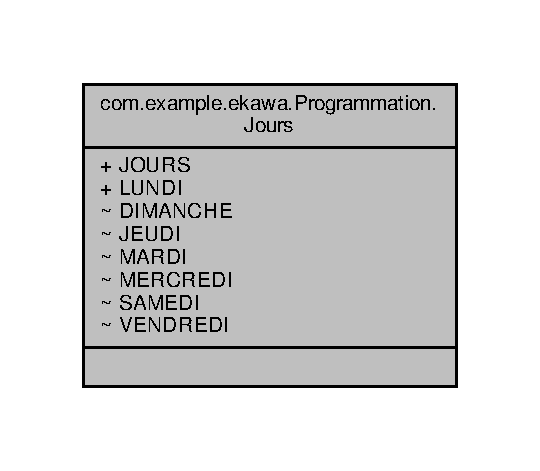
\includegraphics[width=259pt]{classcom_1_1example_1_1ekawa_1_1_programmation_1_1_jours__coll__graph}
\end{center}
\end{figure}
\subsubsection*{Attributs publics statiques}
\begin{DoxyCompactItemize}
\item 
static final String \mbox{[}$\,$\mbox{]} \hyperlink{classcom_1_1example_1_1ekawa_1_1_programmation_1_1_jours_a45d873d90f82a1cdeabeba21a37b7aba}{J\+O\+U\+RS}
\item 
static final int \hyperlink{classcom_1_1example_1_1ekawa_1_1_programmation_1_1_jours_af73668910813425a74baccc5940153ef}{L\+U\+N\+DI} = 0
\end{DoxyCompactItemize}


\subsubsection{Description détaillée}


Définition à la ligne \hyperlink{_programmation_8java_source_l00036}{36} du fichier \hyperlink{_programmation_8java_source}{Programmation.\+java}.



\subsubsection{Documentation des données membres}
\mbox{\Hypertarget{classcom_1_1example_1_1ekawa_1_1_programmation_1_1_jours_a45d873d90f82a1cdeabeba21a37b7aba}\label{classcom_1_1example_1_1ekawa_1_1_programmation_1_1_jours_a45d873d90f82a1cdeabeba21a37b7aba}} 
\index{com\+::example\+::ekawa\+::\+Programmation\+::\+Jours@{com\+::example\+::ekawa\+::\+Programmation\+::\+Jours}!J\+O\+U\+RS@{J\+O\+U\+RS}}
\index{J\+O\+U\+RS@{J\+O\+U\+RS}!com\+::example\+::ekawa\+::\+Programmation\+::\+Jours@{com\+::example\+::ekawa\+::\+Programmation\+::\+Jours}}
\paragraph{\texorpdfstring{J\+O\+U\+RS}{JOURS}}
{\footnotesize\ttfamily final String \mbox{[}$\,$\mbox{]} com.\+example.\+ekawa.\+Programmation.\+Jours.\+J\+O\+U\+RS\hspace{0.3cm}{\ttfamily [static]}}

{\bfseries Valeur initiale \+:}
\begin{DoxyCode}
=
        \{
            \textcolor{stringliteral}{"Lundi"},
            \textcolor{stringliteral}{"Mardi"},
            \textcolor{stringliteral}{"Mercredi"},
            \textcolor{stringliteral}{"Jeudi"},
            \textcolor{stringliteral}{"Vendredi"},
            \textcolor{stringliteral}{"Samedi"},
            \textcolor{stringliteral}{"Dimanche"}
        \}
\end{DoxyCode}


Définition à la ligne \hyperlink{_programmation_8java_source_l00047}{47} du fichier \hyperlink{_programmation_8java_source}{Programmation.\+java}.



Référencé par \hyperlink{_ihm_8java_source_l00190}{com.\+example.\+ekawa.\+Ihm.\+Adaptateur\+Programmer.\+Adaptateur\+Programmer()}, et \hyperlink{_ihm_8java_source_l00727}{com.\+example.\+ekawa.\+Ihm.\+initialiser\+Fenetre\+Programmer()}.

\mbox{\Hypertarget{classcom_1_1example_1_1ekawa_1_1_programmation_1_1_jours_af73668910813425a74baccc5940153ef}\label{classcom_1_1example_1_1ekawa_1_1_programmation_1_1_jours_af73668910813425a74baccc5940153ef}} 
\index{com\+::example\+::ekawa\+::\+Programmation\+::\+Jours@{com\+::example\+::ekawa\+::\+Programmation\+::\+Jours}!L\+U\+N\+DI@{L\+U\+N\+DI}}
\index{L\+U\+N\+DI@{L\+U\+N\+DI}!com\+::example\+::ekawa\+::\+Programmation\+::\+Jours@{com\+::example\+::ekawa\+::\+Programmation\+::\+Jours}}
\paragraph{\texorpdfstring{L\+U\+N\+DI}{LUNDI}}
{\footnotesize\ttfamily final int com.\+example.\+ekawa.\+Programmation.\+Jours.\+L\+U\+N\+DI = 0\hspace{0.3cm}{\ttfamily [static]}}



Définition à la ligne \hyperlink{_programmation_8java_source_l00039}{39} du fichier \hyperlink{_programmation_8java_source}{Programmation.\+java}.



Référencé par \hyperlink{_ihm_8java_source_l00938}{com.\+example.\+ekawa.\+Ihm.\+actualiser\+Page\+Programmer()}.



La documentation de cette classe a été générée à partir du fichier suivant \+:\begin{DoxyCompactItemize}
\item 
\hyperlink{_programmation_8java}{Programmation.\+java}\end{DoxyCompactItemize}

\hypertarget{classcom_1_1example_1_1ekawa_1_1_peripherique}{}\subsection{Référence de la classe com.\+example.\+ekawa.\+Peripherique}
\label{classcom_1_1example_1_1ekawa_1_1_peripherique}\index{com.\+example.\+ekawa.\+Peripherique@{com.\+example.\+ekawa.\+Peripherique}}


Permet le dialogue avec le périphérique Bluetooth de la cafetière.  




Graphe de collaboration de com.\+example.\+ekawa.\+Peripherique\+:\nopagebreak
\begin{figure}[H]
\begin{center}
\leavevmode
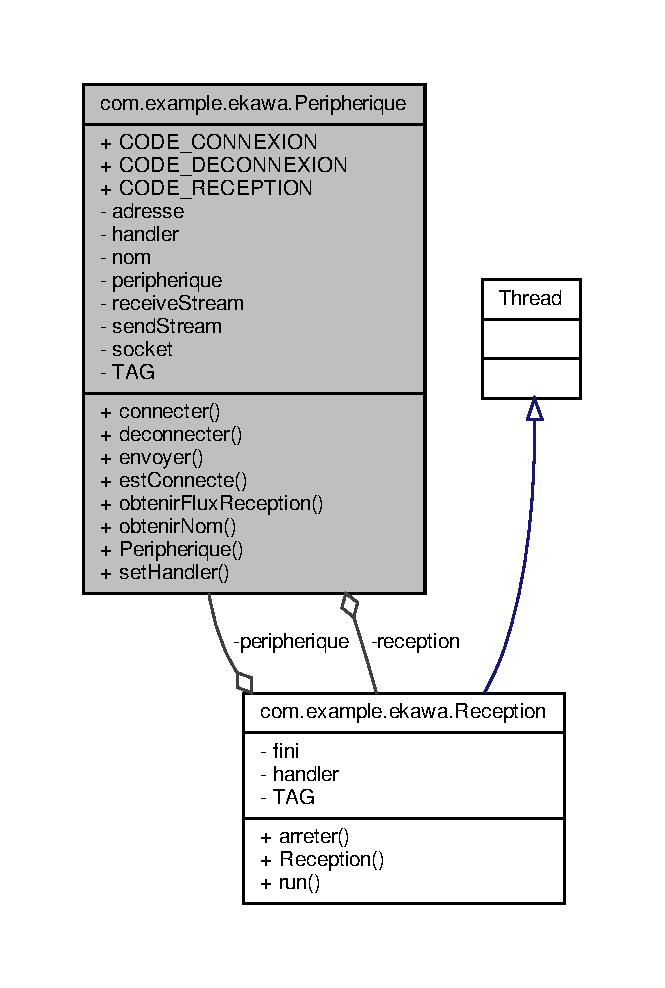
\includegraphics[width=319pt]{classcom_1_1example_1_1ekawa_1_1_peripherique__coll__graph}
\end{center}
\end{figure}
\subsubsection*{Fonctions membres publiques}
\begin{DoxyCompactItemize}
\item 
void \hyperlink{classcom_1_1example_1_1ekawa_1_1_peripherique_aeec8c1b360496726a5aecd6c129de81b}{connecter} ()
\begin{DoxyCompactList}\small\item\em Méthode qui permet de connecter le bluetooth à la cafetière. \end{DoxyCompactList}\item 
void \hyperlink{classcom_1_1example_1_1ekawa_1_1_peripherique_aadfd24f4d783a7834c044041c7c035bb}{deconnecter} ()
\begin{DoxyCompactList}\small\item\em Méthode qui permet de deconnecter le bluetooth de la cafetière. \end{DoxyCompactList}\item 
boolean \hyperlink{classcom_1_1example_1_1ekawa_1_1_peripherique_ac1361bc1a445b00c4c7ebb56dfee274d}{envoyer} (String trame)
\begin{DoxyCompactList}\small\item\em Méthode qui permet d\textquotesingle{}envoyer des trames à la cafetière. \end{DoxyCompactList}\item 
boolean \hyperlink{classcom_1_1example_1_1ekawa_1_1_peripherique_a963c20e3fba4ed926e9dee972e3b6b39}{est\+Connecte} ()
\item 
Input\+Stream \hyperlink{classcom_1_1example_1_1ekawa_1_1_peripherique_a8b88d0a0d9e0c1b1aae04ba7c9d24619}{obtenir\+Flux\+Reception} ()
\item 
String \hyperlink{classcom_1_1example_1_1ekawa_1_1_peripherique_ad54cfafe03dfcf18cbd9b20602c4d86e}{obtenir\+Nom} ()
\item 
\hyperlink{classcom_1_1example_1_1ekawa_1_1_peripherique_af952f48e767069b44804a96119bf3c75}{Peripherique} (Bluetooth\+Device \hyperlink{classcom_1_1example_1_1ekawa_1_1_peripherique_ab509bd2180c53845197423813a97f025}{peripherique}, Handler \hyperlink{classcom_1_1example_1_1ekawa_1_1_peripherique_ab6a0c0cae2eb087315d0d04d1cf6c3dc}{handler})
\begin{DoxyCompactList}\small\item\em Constructeur de la classe \hyperlink{classcom_1_1example_1_1ekawa_1_1_peripherique}{Peripherique}. \end{DoxyCompactList}\item 
void \hyperlink{classcom_1_1example_1_1ekawa_1_1_peripherique_a2cfa1b391efb3f2e7a78e761e965e7e3}{set\+Handler} (Handler \hyperlink{classcom_1_1example_1_1ekawa_1_1_peripherique_ab6a0c0cae2eb087315d0d04d1cf6c3dc}{handler})
\end{DoxyCompactItemize}
\subsubsection*{Attributs publics statiques}
\begin{DoxyCompactItemize}
\item 
static final int \hyperlink{classcom_1_1example_1_1ekawa_1_1_peripherique_addb8ee767dc82567360551db1004463e}{C\+O\+D\+E\+\_\+\+C\+O\+N\+N\+E\+X\+I\+ON} = 0
\item 
static final int \hyperlink{classcom_1_1example_1_1ekawa_1_1_peripherique_a99f0e30a113d64b30598c6305657dcee}{C\+O\+D\+E\+\_\+\+D\+E\+C\+O\+N\+N\+E\+X\+I\+ON} = 2
\item 
static final int \hyperlink{classcom_1_1example_1_1ekawa_1_1_peripherique_a532f5da1747b68217b8764db9b85e845}{C\+O\+D\+E\+\_\+\+R\+E\+C\+E\+P\+T\+I\+ON} = 1
\end{DoxyCompactItemize}
\subsubsection*{Attributs privés}
\begin{DoxyCompactItemize}
\item 
String \hyperlink{classcom_1_1example_1_1ekawa_1_1_peripherique_a2617309b5112a289fcd9f9570154341c}{adresse}
\item 
Handler \hyperlink{classcom_1_1example_1_1ekawa_1_1_peripherique_ab6a0c0cae2eb087315d0d04d1cf6c3dc}{handler}
\item 
String \hyperlink{classcom_1_1example_1_1ekawa_1_1_peripherique_a0fb529bb80d55dd616821bce74a2af8c}{nom}
\item 
Bluetooth\+Device \hyperlink{classcom_1_1example_1_1ekawa_1_1_peripherique_ab509bd2180c53845197423813a97f025}{peripherique} = null
\item 
Input\+Stream \hyperlink{classcom_1_1example_1_1ekawa_1_1_peripherique_af46a939491178c90c1ecd75dd781f4b6}{receive\+Stream} = null
\item 
\hyperlink{classcom_1_1example_1_1ekawa_1_1_reception}{Reception} \hyperlink{classcom_1_1example_1_1ekawa_1_1_peripherique_a0192ad260e727ed46efa968a79364338}{reception} = null
\item 
Output\+Stream \hyperlink{classcom_1_1example_1_1ekawa_1_1_peripherique_a9bacd88ef2a26eedac31fda999734639}{send\+Stream} = null
\item 
Bluetooth\+Socket \hyperlink{classcom_1_1example_1_1ekawa_1_1_peripherique_a00e15bc5bdafff61d45d4e39d7dd21e0}{socket} = null
\end{DoxyCompactItemize}
\subsubsection*{Attributs privés statiques}
\begin{DoxyCompactItemize}
\item 
static final String \hyperlink{classcom_1_1example_1_1ekawa_1_1_peripherique_a80ad0e52c530c7dc114109ff777ae975}{T\+AG} = \char`\"{}Peripherique\char`\"{}
\begin{DoxyCompactList}\small\item\em T\+AG pour les logs. \end{DoxyCompactList}\end{DoxyCompactItemize}


\subsubsection{Description détaillée}
Permet le dialogue avec le périphérique Bluetooth de la cafetière. 

Définition à la ligne \hyperlink{_peripherique_8java_source_l00029}{29} du fichier \hyperlink{_peripherique_8java_source}{Peripherique.\+java}.



\subsubsection{Documentation des constructeurs et destructeur}
\mbox{\Hypertarget{classcom_1_1example_1_1ekawa_1_1_peripherique_af952f48e767069b44804a96119bf3c75}\label{classcom_1_1example_1_1ekawa_1_1_peripherique_af952f48e767069b44804a96119bf3c75}} 
\index{com\+::example\+::ekawa\+::\+Peripherique@{com\+::example\+::ekawa\+::\+Peripherique}!Peripherique@{Peripherique}}
\index{Peripherique@{Peripherique}!com\+::example\+::ekawa\+::\+Peripherique@{com\+::example\+::ekawa\+::\+Peripherique}}
\paragraph{\texorpdfstring{Peripherique()}{Peripherique()}}
{\footnotesize\ttfamily com.\+example.\+ekawa.\+Peripherique.\+Peripherique (\begin{DoxyParamCaption}\item[{Bluetooth\+Device}]{peripherique,  }\item[{Handler}]{handler }\end{DoxyParamCaption})}



Constructeur de la classe \hyperlink{classcom_1_1example_1_1ekawa_1_1_peripherique}{Peripherique}. 



Définition à la ligne \hyperlink{_peripherique_8java_source_l00052}{52} du fichier \hyperlink{_peripherique_8java_source}{Peripherique.\+java}.



Références \hyperlink{_peripherique_8java_source_l00047}{com.\+example.\+ekawa.\+Peripherique.\+handler}, \hyperlink{_peripherique_8java_source_l00244}{com.\+example.\+ekawa.\+Peripherique.\+obtenir\+Nom()}, et \hyperlink{_peripherique_8java_source_l00039}{com.\+example.\+ekawa.\+Peripherique.\+peripherique}.


\begin{DoxyCode}
00053     \{
00054         Log.d(\hyperlink{classcom_1_1example_1_1ekawa_1_1_peripherique_a80ad0e52c530c7dc114109ff777ae975}{TAG},\textcolor{stringliteral}{"Peripherique()"});
00055         \textcolor{keywordflow}{if} (\hyperlink{classcom_1_1example_1_1ekawa_1_1_peripherique_ab509bd2180c53845197423813a97f025}{peripherique} != null)
00056         \{
00057             this.\hyperlink{classcom_1_1example_1_1ekawa_1_1_peripherique_ab509bd2180c53845197423813a97f025}{peripherique} = \hyperlink{classcom_1_1example_1_1ekawa_1_1_peripherique_ab509bd2180c53845197423813a97f025}{peripherique};
00058             this.\hyperlink{classcom_1_1example_1_1ekawa_1_1_peripherique_a0fb529bb80d55dd616821bce74a2af8c}{nom} = \hyperlink{classcom_1_1example_1_1ekawa_1_1_peripherique_ab509bd2180c53845197423813a97f025}{peripherique}.getName();
00059             this.\hyperlink{classcom_1_1example_1_1ekawa_1_1_peripherique_a2617309b5112a289fcd9f9570154341c}{adresse} = \hyperlink{classcom_1_1example_1_1ekawa_1_1_peripherique_ab509bd2180c53845197423813a97f025}{peripherique}.getAddress();
00060             this.\hyperlink{classcom_1_1example_1_1ekawa_1_1_peripherique_ab6a0c0cae2eb087315d0d04d1cf6c3dc}{handler} = \hyperlink{classcom_1_1example_1_1ekawa_1_1_peripherique_ab6a0c0cae2eb087315d0d04d1cf6c3dc}{handler};
00061 
00062             \textcolor{keywordflow}{try}
00063             \{
00064                 \hyperlink{classcom_1_1example_1_1ekawa_1_1_peripherique_a00e15bc5bdafff61d45d4e39d7dd21e0}{socket} = \hyperlink{classcom_1_1example_1_1ekawa_1_1_peripherique_ab509bd2180c53845197423813a97f025}{peripherique}.createRfcommSocketToServiceRecord(UUID.fromString(\textcolor{stringliteral}{"
      00001101-0000-1000-8000-00805F9B34FB"}));
00065                 \hyperlink{classcom_1_1example_1_1ekawa_1_1_peripherique_af46a939491178c90c1ecd75dd781f4b6}{receiveStream} = \hyperlink{classcom_1_1example_1_1ekawa_1_1_peripherique_a00e15bc5bdafff61d45d4e39d7dd21e0}{socket}.getInputStream();
00066                 \hyperlink{classcom_1_1example_1_1ekawa_1_1_peripherique_a9bacd88ef2a26eedac31fda999734639}{sendStream} = \hyperlink{classcom_1_1example_1_1ekawa_1_1_peripherique_a00e15bc5bdafff61d45d4e39d7dd21e0}{socket}.getOutputStream();
00067             \}
00068             \textcolor{keywordflow}{catch}(IOException e)
00069             \{
00070                 e.printStackTrace();
00071                 \hyperlink{classcom_1_1example_1_1ekawa_1_1_peripherique_a00e15bc5bdafff61d45d4e39d7dd21e0}{socket} = null;
00072                 Log.d(\hyperlink{classcom_1_1example_1_1ekawa_1_1_peripherique_a80ad0e52c530c7dc114109ff777ae975}{TAG},\textcolor{stringliteral}{"Erreur création socket !"});
00073             \}
00074         \}
00075         \textcolor{keywordflow}{else}
00076         \{
00077             this.\hyperlink{classcom_1_1example_1_1ekawa_1_1_peripherique_ab509bd2180c53845197423813a97f025}{peripherique} = \hyperlink{classcom_1_1example_1_1ekawa_1_1_peripherique_ab509bd2180c53845197423813a97f025}{peripherique};
00078             this.\hyperlink{classcom_1_1example_1_1ekawa_1_1_peripherique_a0fb529bb80d55dd616821bce74a2af8c}{nom} = \textcolor{stringliteral}{"Aucun"};
00079             this.\hyperlink{classcom_1_1example_1_1ekawa_1_1_peripherique_a2617309b5112a289fcd9f9570154341c}{adresse} = \textcolor{stringliteral}{""};
00080             this.\hyperlink{classcom_1_1example_1_1ekawa_1_1_peripherique_ab6a0c0cae2eb087315d0d04d1cf6c3dc}{handler} = null;
00081         \}
00082 
00083         \textcolor{keywordflow}{if}(\hyperlink{classcom_1_1example_1_1ekawa_1_1_peripherique_a00e15bc5bdafff61d45d4e39d7dd21e0}{socket} != null)
00084         \{
00085             \hyperlink{classcom_1_1example_1_1ekawa_1_1_peripherique_a0192ad260e727ed46efa968a79364338}{reception} = \textcolor{keyword}{new} Reception(\textcolor{keyword}{this}, \hyperlink{classcom_1_1example_1_1ekawa_1_1_peripherique_ab6a0c0cae2eb087315d0d04d1cf6c3dc}{handler});
00086             Log.v(\hyperlink{classcom_1_1example_1_1ekawa_1_1_peripherique_a80ad0e52c530c7dc114109ff777ae975}{TAG}, \textcolor{stringliteral}{"Périphérique "} + \hyperlink{classcom_1_1example_1_1ekawa_1_1_peripherique_ad54cfafe03dfcf18cbd9b20602c4d86e}{obtenirNom}() + \textcolor{stringliteral}{" prêt"});
00087         \}
00088     \}
\end{DoxyCode}


\subsubsection{Documentation des fonctions membres}
\mbox{\Hypertarget{classcom_1_1example_1_1ekawa_1_1_peripherique_aeec8c1b360496726a5aecd6c129de81b}\label{classcom_1_1example_1_1ekawa_1_1_peripherique_aeec8c1b360496726a5aecd6c129de81b}} 
\index{com\+::example\+::ekawa\+::\+Peripherique@{com\+::example\+::ekawa\+::\+Peripherique}!connecter@{connecter}}
\index{connecter@{connecter}!com\+::example\+::ekawa\+::\+Peripherique@{com\+::example\+::ekawa\+::\+Peripherique}}
\paragraph{\texorpdfstring{connecter()}{connecter()}}
{\footnotesize\ttfamily void com.\+example.\+ekawa.\+Peripherique.\+connecter (\begin{DoxyParamCaption}{ }\end{DoxyParamCaption})}



Méthode qui permet de connecter le bluetooth à la cafetière. 



Définition à la ligne \hyperlink{_peripherique_8java_source_l00101}{101} du fichier \hyperlink{_peripherique_8java_source}{Peripherique.\+java}.



Références \hyperlink{_peripherique_8java_source_l00033}{com.\+example.\+ekawa.\+Peripherique.\+C\+O\+D\+E\+\_\+\+C\+O\+N\+N\+E\+X\+I\+ON}, et \hyperlink{_peripherique_8java_source_l00244}{com.\+example.\+ekawa.\+Peripherique.\+obtenir\+Nom()}.



Référencé par \hyperlink{_communication_8java_source_l00276}{com.\+example.\+ekawa.\+Communication.\+chercher\+Cafetiere()}, et \hyperlink{_communication_8java_source_l00078}{com.\+example.\+ekawa.\+Communication.\+detection\+Changement\+Etat\+Bluetooth()}.


\begin{DoxyCode}
00102     \{
00103         \textcolor{keywordflow}{if}(\hyperlink{classcom_1_1example_1_1ekawa_1_1_peripherique_ab509bd2180c53845197423813a97f025}{peripherique} == null)
00104             \textcolor{keywordflow}{return};
00105 
00106         \textcolor{keyword}{new} \hyperlink{class_thread}{Thread}()
00107         \{
00108             @Override \textcolor{keyword}{public} \textcolor{keywordtype}{void} run()
00109             \{
00110                 \textcolor{keywordflow}{try}
00111                 \{
00112                     \textcolor{keywordflow}{if}(\hyperlink{classcom_1_1example_1_1ekawa_1_1_peripherique_a00e15bc5bdafff61d45d4e39d7dd21e0}{socket} != null)
00113                     \{
00114                         \textcolor{keywordflow}{if}(!\hyperlink{classcom_1_1example_1_1ekawa_1_1_peripherique_a00e15bc5bdafff61d45d4e39d7dd21e0}{socket}.isConnected())
00115                         \{
00116                             Log.d(\hyperlink{classcom_1_1example_1_1ekawa_1_1_peripherique_a80ad0e52c530c7dc114109ff777ae975}{TAG}, \textcolor{stringliteral}{"Socket connexion à "} + \hyperlink{classcom_1_1example_1_1ekawa_1_1_peripherique_ad54cfafe03dfcf18cbd9b20602c4d86e}{obtenirNom}());
00117                             \hyperlink{classcom_1_1example_1_1ekawa_1_1_peripherique_a00e15bc5bdafff61d45d4e39d7dd21e0}{socket}.connect();
00118                         \}
00119 
00120                         \textcolor{keywordflow}{if}(\hyperlink{classcom_1_1example_1_1ekawa_1_1_peripherique_a00e15bc5bdafff61d45d4e39d7dd21e0}{socket}.isConnected())
00121                         \{
00122                             Log.d(\hyperlink{classcom_1_1example_1_1ekawa_1_1_peripherique_a80ad0e52c530c7dc114109ff777ae975}{TAG}, \textcolor{stringliteral}{"Socket connecté à "} + \hyperlink{classcom_1_1example_1_1ekawa_1_1_peripherique_ad54cfafe03dfcf18cbd9b20602c4d86e}{obtenirNom}());
00123                             \textcolor{keywordflow}{if}(\hyperlink{classcom_1_1example_1_1ekawa_1_1_peripherique_ab6a0c0cae2eb087315d0d04d1cf6c3dc}{handler} != null)
00124                             \{
00125                                 Message msg = Message.obtain();
00126                                 msg.what = \hyperlink{classcom_1_1example_1_1ekawa_1_1_peripherique_addb8ee767dc82567360551db1004463e}{CODE\_CONNEXION};
00127                                 \hyperlink{classcom_1_1example_1_1ekawa_1_1_peripherique_ab6a0c0cae2eb087315d0d04d1cf6c3dc}{handler}.sendMessage(msg);
00128                             \}
00129                         \}
00130 
00131                         \textcolor{keywordflow}{if} (\hyperlink{classcom_1_1example_1_1ekawa_1_1_peripherique_a0192ad260e727ed46efa968a79364338}{reception} != null)
00132                         \{
00133                             \hyperlink{classcom_1_1example_1_1ekawa_1_1_peripherique_a0192ad260e727ed46efa968a79364338}{reception}.start();
00134                             Log.d(\hyperlink{classcom_1_1example_1_1ekawa_1_1_peripherique_a80ad0e52c530c7dc114109ff777ae975}{TAG}, \textcolor{stringliteral}{"Démarrage thread réception"});
00135                         \}
00136                     \}
00137                 \}
00138                 \textcolor{keywordflow}{catch} (IOException e)
00139                 \{
00140                     Log.d(\hyperlink{classcom_1_1example_1_1ekawa_1_1_peripherique_a80ad0e52c530c7dc114109ff777ae975}{TAG},\textcolor{stringliteral}{"Erreur connexion socket !"});
00141                     e.printStackTrace();
00142                 \}
00143             \}
00144         \}.start();
00145     \}
\end{DoxyCode}
\mbox{\Hypertarget{classcom_1_1example_1_1ekawa_1_1_peripherique_aadfd24f4d783a7834c044041c7c035bb}\label{classcom_1_1example_1_1ekawa_1_1_peripherique_aadfd24f4d783a7834c044041c7c035bb}} 
\index{com\+::example\+::ekawa\+::\+Peripherique@{com\+::example\+::ekawa\+::\+Peripherique}!deconnecter@{deconnecter}}
\index{deconnecter@{deconnecter}!com\+::example\+::ekawa\+::\+Peripherique@{com\+::example\+::ekawa\+::\+Peripherique}}
\paragraph{\texorpdfstring{deconnecter()}{deconnecter()}}
{\footnotesize\ttfamily void com.\+example.\+ekawa.\+Peripherique.\+deconnecter (\begin{DoxyParamCaption}{ }\end{DoxyParamCaption})}



Méthode qui permet de deconnecter le bluetooth de la cafetière. 



Définition à la ligne \hyperlink{_peripherique_8java_source_l00150}{150} du fichier \hyperlink{_peripherique_8java_source}{Peripherique.\+java}.



Références \hyperlink{_reception_8java_source_l00088}{com.\+example.\+ekawa.\+Reception.\+arreter()}, \hyperlink{_peripherique_8java_source_l00035}{com.\+example.\+ekawa.\+Peripherique.\+C\+O\+D\+E\+\_\+\+D\+E\+C\+O\+N\+N\+E\+X\+I\+ON}, et \hyperlink{_peripherique_8java_source_l00244}{com.\+example.\+ekawa.\+Peripherique.\+obtenir\+Nom()}.



Référencé par \hyperlink{_communication_8java_source_l00250}{com.\+example.\+ekawa.\+Communication.\+deconnecter()}.


\begin{DoxyCode}
00151     \{
00152         \textcolor{keywordflow}{if}(\hyperlink{classcom_1_1example_1_1ekawa_1_1_peripherique_ab509bd2180c53845197423813a97f025}{peripherique} == null)
00153             \textcolor{keywordflow}{return};
00154 
00155         \textcolor{keyword}{new} \hyperlink{class_thread}{Thread}()
00156         \{
00157             @Override \textcolor{keyword}{public} \textcolor{keywordtype}{void} run()
00158             \{
00159             \textcolor{keywordflow}{try}
00160             \{
00161                 \textcolor{keywordflow}{if} (\hyperlink{classcom_1_1example_1_1ekawa_1_1_peripherique_a0192ad260e727ed46efa968a79364338}{reception} != null)
00162                 \{
00163                     Log.d(\hyperlink{classcom_1_1example_1_1ekawa_1_1_peripherique_a80ad0e52c530c7dc114109ff777ae975}{TAG},\textcolor{stringliteral}{"Arrêt thread réception"});
00164                     \hyperlink{classcom_1_1example_1_1ekawa_1_1_peripherique_a0192ad260e727ed46efa968a79364338}{reception}.\hyperlink{classcom_1_1example_1_1ekawa_1_1_reception_a844c65410aaeee936f6b0d44f9df56db}{arreter}();
00165                     \hyperlink{classcom_1_1example_1_1ekawa_1_1_peripherique_af46a939491178c90c1ecd75dd781f4b6}{receiveStream}.close();
00166                     \hyperlink{classcom_1_1example_1_1ekawa_1_1_peripherique_a9bacd88ef2a26eedac31fda999734639}{sendStream}.close();
00167                     \textcolor{keywordflow}{if} (\hyperlink{classcom_1_1example_1_1ekawa_1_1_peripherique_a00e15bc5bdafff61d45d4e39d7dd21e0}{socket} != null)
00168                     \{
00169                         Log.d(\hyperlink{classcom_1_1example_1_1ekawa_1_1_peripherique_a80ad0e52c530c7dc114109ff777ae975}{TAG}, \textcolor{stringliteral}{"Socket déconnexion de "} + \hyperlink{classcom_1_1example_1_1ekawa_1_1_peripherique_ad54cfafe03dfcf18cbd9b20602c4d86e}{obtenirNom}());
00170                         \hyperlink{classcom_1_1example_1_1ekawa_1_1_peripherique_a00e15bc5bdafff61d45d4e39d7dd21e0}{socket}.close();
00171 
00172                         \textcolor{keywordflow}{if} (!\hyperlink{classcom_1_1example_1_1ekawa_1_1_peripherique_a00e15bc5bdafff61d45d4e39d7dd21e0}{socket}.isConnected())
00173                         \{
00174                             Log.d(\hyperlink{classcom_1_1example_1_1ekawa_1_1_peripherique_a80ad0e52c530c7dc114109ff777ae975}{TAG}, \textcolor{stringliteral}{"Socket déconnecté de "} + \hyperlink{classcom_1_1example_1_1ekawa_1_1_peripherique_ad54cfafe03dfcf18cbd9b20602c4d86e}{obtenirNom}());
00175                             \textcolor{keywordflow}{if} (\hyperlink{classcom_1_1example_1_1ekawa_1_1_peripherique_ab6a0c0cae2eb087315d0d04d1cf6c3dc}{handler} != null)
00176                             \{
00177                                 Message msg = Message.obtain();
00178                                 msg.what = \hyperlink{classcom_1_1example_1_1ekawa_1_1_peripherique_a99f0e30a113d64b30598c6305657dcee}{CODE\_DECONNEXION};
00179                                 \hyperlink{classcom_1_1example_1_1ekawa_1_1_peripherique_ab6a0c0cae2eb087315d0d04d1cf6c3dc}{handler}.sendMessage(msg);
00180                             \}
00181                         \}
00182                     \}
00183                 \}
00184             \}
00185             \textcolor{keywordflow}{catch} (IOException e)
00186             \{
00187                 Log.d(\hyperlink{classcom_1_1example_1_1ekawa_1_1_peripherique_a80ad0e52c530c7dc114109ff777ae975}{TAG},\textcolor{stringliteral}{"Erreur fermeture socket !"});
00188                 e.printStackTrace();
00189             \}
00190             \}
00191         \}.start();
00192     \}
\end{DoxyCode}
\mbox{\Hypertarget{classcom_1_1example_1_1ekawa_1_1_peripherique_ac1361bc1a445b00c4c7ebb56dfee274d}\label{classcom_1_1example_1_1ekawa_1_1_peripherique_ac1361bc1a445b00c4c7ebb56dfee274d}} 
\index{com\+::example\+::ekawa\+::\+Peripherique@{com\+::example\+::ekawa\+::\+Peripherique}!envoyer@{envoyer}}
\index{envoyer@{envoyer}!com\+::example\+::ekawa\+::\+Peripherique@{com\+::example\+::ekawa\+::\+Peripherique}}
\paragraph{\texorpdfstring{envoyer()}{envoyer()}}
{\footnotesize\ttfamily boolean com.\+example.\+ekawa.\+Peripherique.\+envoyer (\begin{DoxyParamCaption}\item[{String}]{trame }\end{DoxyParamCaption})}



Méthode qui permet d\textquotesingle{}envoyer des trames à la cafetière. 



Définition à la ligne \hyperlink{_peripherique_8java_source_l00197}{197} du fichier \hyperlink{_peripherique_8java_source}{Peripherique.\+java}.



Référencé par \hyperlink{_communication_8java_source_l00309}{com.\+example.\+ekawa.\+Communication.\+envoyer\+Trame()}.


\begin{DoxyCode}
00198     \{
00199         \textcolor{keyword}{final} String trameEnvoyee = trame;
00200 
00201         \textcolor{keywordflow}{if}(\hyperlink{classcom_1_1example_1_1ekawa_1_1_peripherique_a00e15bc5bdafff61d45d4e39d7dd21e0}{socket} == null)
00202             \textcolor{keywordflow}{return} \textcolor{keyword}{false};
00203 
00204         \textcolor{keywordflow}{if}(!\hyperlink{classcom_1_1example_1_1ekawa_1_1_peripherique_a00e15bc5bdafff61d45d4e39d7dd21e0}{socket}.isConnected())
00205             \textcolor{keywordflow}{return} \textcolor{keyword}{false};
00206 
00207         \textcolor{keyword}{new} \hyperlink{class_thread}{Thread}()
00208         \{
00209             @Override \textcolor{keyword}{public} \textcolor{keywordtype}{void} run()
00210             \{
00211                 \textcolor{keywordflow}{try}
00212                 \{
00213                     \textcolor{keywordflow}{if}(\hyperlink{classcom_1_1example_1_1ekawa_1_1_peripherique_a00e15bc5bdafff61d45d4e39d7dd21e0}{socket}.isConnected())
00214                     \{
00215                         \hyperlink{classcom_1_1example_1_1ekawa_1_1_peripherique_a9bacd88ef2a26eedac31fda999734639}{sendStream}.write(trameEnvoyee.getBytes());
00216                         \hyperlink{classcom_1_1example_1_1ekawa_1_1_peripherique_a9bacd88ef2a26eedac31fda999734639}{sendStream}.flush();
00217                         Log.d(\hyperlink{classcom_1_1example_1_1ekawa_1_1_peripherique_a80ad0e52c530c7dc114109ff777ae975}{TAG}, \textcolor{stringliteral}{"envoyer() : "} + trameEnvoyee);
00218                     \}
00219                 \}
00220                 \textcolor{keywordflow}{catch} (IOException e)
00221                 \{
00222                     Log.d(\hyperlink{classcom_1_1example_1_1ekawa_1_1_peripherique_a80ad0e52c530c7dc114109ff777ae975}{TAG},\textcolor{stringliteral}{"Erreur écriture socket !"});
00223                     e.printStackTrace();
00224                 \}
00225             \}
00226         \}.start();
00227 
00228         \textcolor{keywordflow}{return} \textcolor{keyword}{true};
00229     \}
\end{DoxyCode}
\mbox{\Hypertarget{classcom_1_1example_1_1ekawa_1_1_peripherique_a963c20e3fba4ed926e9dee972e3b6b39}\label{classcom_1_1example_1_1ekawa_1_1_peripherique_a963c20e3fba4ed926e9dee972e3b6b39}} 
\index{com\+::example\+::ekawa\+::\+Peripherique@{com\+::example\+::ekawa\+::\+Peripherique}!est\+Connecte@{est\+Connecte}}
\index{est\+Connecte@{est\+Connecte}!com\+::example\+::ekawa\+::\+Peripherique@{com\+::example\+::ekawa\+::\+Peripherique}}
\paragraph{\texorpdfstring{est\+Connecte()}{estConnecte()}}
{\footnotesize\ttfamily boolean com.\+example.\+ekawa.\+Peripherique.\+est\+Connecte (\begin{DoxyParamCaption}{ }\end{DoxyParamCaption})}



Définition à la ligne \hyperlink{_peripherique_8java_source_l00234}{234} du fichier \hyperlink{_peripherique_8java_source}{Peripherique.\+java}.



Référencé par \hyperlink{_communication_8java_source_l00276}{com.\+example.\+ekawa.\+Communication.\+chercher\+Cafetiere()}, et \hyperlink{_communication_8java_source_l00078}{com.\+example.\+ekawa.\+Communication.\+detection\+Changement\+Etat\+Bluetooth()}.


\begin{DoxyCode}
00235     \{
00236         \textcolor{keywordflow}{if}(\hyperlink{classcom_1_1example_1_1ekawa_1_1_peripherique_a00e15bc5bdafff61d45d4e39d7dd21e0}{socket} != null)
00237             \textcolor{keywordflow}{return} \hyperlink{classcom_1_1example_1_1ekawa_1_1_peripherique_a00e15bc5bdafff61d45d4e39d7dd21e0}{socket}.isConnected();
00238         \textcolor{keywordflow}{return} \textcolor{keyword}{false};
00239     \}
\end{DoxyCode}
\mbox{\Hypertarget{classcom_1_1example_1_1ekawa_1_1_peripherique_a8b88d0a0d9e0c1b1aae04ba7c9d24619}\label{classcom_1_1example_1_1ekawa_1_1_peripherique_a8b88d0a0d9e0c1b1aae04ba7c9d24619}} 
\index{com\+::example\+::ekawa\+::\+Peripherique@{com\+::example\+::ekawa\+::\+Peripherique}!obtenir\+Flux\+Reception@{obtenir\+Flux\+Reception}}
\index{obtenir\+Flux\+Reception@{obtenir\+Flux\+Reception}!com\+::example\+::ekawa\+::\+Peripherique@{com\+::example\+::ekawa\+::\+Peripherique}}
\paragraph{\texorpdfstring{obtenir\+Flux\+Reception()}{obtenirFluxReception()}}
{\footnotesize\ttfamily Input\+Stream com.\+example.\+ekawa.\+Peripherique.\+obtenir\+Flux\+Reception (\begin{DoxyParamCaption}{ }\end{DoxyParamCaption})}



Définition à la ligne \hyperlink{_peripherique_8java_source_l00252}{252} du fichier \hyperlink{_peripherique_8java_source}{Peripherique.\+java}.



Références \hyperlink{_peripherique_8java_source_l00042}{com.\+example.\+ekawa.\+Peripherique.\+receive\+Stream}.



Référencé par \hyperlink{_reception_8java_source_l00043}{com.\+example.\+ekawa.\+Reception.\+run()}.


\begin{DoxyCode}
00253     \{
00254         \textcolor{keywordflow}{return} \hyperlink{classcom_1_1example_1_1ekawa_1_1_peripherique_af46a939491178c90c1ecd75dd781f4b6}{receiveStream};
00255     \}
\end{DoxyCode}
\mbox{\Hypertarget{classcom_1_1example_1_1ekawa_1_1_peripherique_ad54cfafe03dfcf18cbd9b20602c4d86e}\label{classcom_1_1example_1_1ekawa_1_1_peripherique_ad54cfafe03dfcf18cbd9b20602c4d86e}} 
\index{com\+::example\+::ekawa\+::\+Peripherique@{com\+::example\+::ekawa\+::\+Peripherique}!obtenir\+Nom@{obtenir\+Nom}}
\index{obtenir\+Nom@{obtenir\+Nom}!com\+::example\+::ekawa\+::\+Peripherique@{com\+::example\+::ekawa\+::\+Peripherique}}
\paragraph{\texorpdfstring{obtenir\+Nom()}{obtenirNom()}}
{\footnotesize\ttfamily String com.\+example.\+ekawa.\+Peripherique.\+obtenir\+Nom (\begin{DoxyParamCaption}{ }\end{DoxyParamCaption})}



Définition à la ligne \hyperlink{_peripherique_8java_source_l00244}{244} du fichier \hyperlink{_peripherique_8java_source}{Peripherique.\+java}.



Références \hyperlink{_peripherique_8java_source_l00037}{com.\+example.\+ekawa.\+Peripherique.\+nom}.



Référencé par \hyperlink{_communication_8java_source_l00276}{com.\+example.\+ekawa.\+Communication.\+chercher\+Cafetiere()}, \hyperlink{_peripherique_8java_source_l00101}{com.\+example.\+ekawa.\+Peripherique.\+connecter()}, \hyperlink{_peripherique_8java_source_l00150}{com.\+example.\+ekawa.\+Peripherique.\+deconnecter()}, \hyperlink{_communication_8java_source_l00379}{com.\+example.\+ekawa.\+Communication.\+obtenir\+Nom\+Peripherique()}, et \hyperlink{_peripherique_8java_source_l00052}{com.\+example.\+ekawa.\+Peripherique.\+Peripherique()}.


\begin{DoxyCode}
00245     \{
00246         \textcolor{keywordflow}{return} \hyperlink{classcom_1_1example_1_1ekawa_1_1_peripherique_a0fb529bb80d55dd616821bce74a2af8c}{nom};
00247     \}
\end{DoxyCode}
\mbox{\Hypertarget{classcom_1_1example_1_1ekawa_1_1_peripherique_a2cfa1b391efb3f2e7a78e761e965e7e3}\label{classcom_1_1example_1_1ekawa_1_1_peripherique_a2cfa1b391efb3f2e7a78e761e965e7e3}} 
\index{com\+::example\+::ekawa\+::\+Peripherique@{com\+::example\+::ekawa\+::\+Peripherique}!set\+Handler@{set\+Handler}}
\index{set\+Handler@{set\+Handler}!com\+::example\+::ekawa\+::\+Peripherique@{com\+::example\+::ekawa\+::\+Peripherique}}
\paragraph{\texorpdfstring{set\+Handler()}{setHandler()}}
{\footnotesize\ttfamily void com.\+example.\+ekawa.\+Peripherique.\+set\+Handler (\begin{DoxyParamCaption}\item[{Handler}]{handler }\end{DoxyParamCaption})}



Définition à la ligne \hyperlink{_peripherique_8java_source_l00093}{93} du fichier \hyperlink{_peripherique_8java_source}{Peripherique.\+java}.



Références \hyperlink{_peripherique_8java_source_l00047}{com.\+example.\+ekawa.\+Peripherique.\+handler}.


\begin{DoxyCode}
00094     \{
00095         this.\hyperlink{classcom_1_1example_1_1ekawa_1_1_peripherique_ab6a0c0cae2eb087315d0d04d1cf6c3dc}{handler} = \hyperlink{classcom_1_1example_1_1ekawa_1_1_peripherique_ab6a0c0cae2eb087315d0d04d1cf6c3dc}{handler};
00096     \}
\end{DoxyCode}


\subsubsection{Documentation des données membres}
\mbox{\Hypertarget{classcom_1_1example_1_1ekawa_1_1_peripherique_a2617309b5112a289fcd9f9570154341c}\label{classcom_1_1example_1_1ekawa_1_1_peripherique_a2617309b5112a289fcd9f9570154341c}} 
\index{com\+::example\+::ekawa\+::\+Peripherique@{com\+::example\+::ekawa\+::\+Peripherique}!adresse@{adresse}}
\index{adresse@{adresse}!com\+::example\+::ekawa\+::\+Peripherique@{com\+::example\+::ekawa\+::\+Peripherique}}
\paragraph{\texorpdfstring{adresse}{adresse}}
{\footnotesize\ttfamily String com.\+example.\+ekawa.\+Peripherique.\+adresse\hspace{0.3cm}{\ttfamily [private]}}



Définition à la ligne \hyperlink{_peripherique_8java_source_l00038}{38} du fichier \hyperlink{_peripherique_8java_source}{Peripherique.\+java}.

\mbox{\Hypertarget{classcom_1_1example_1_1ekawa_1_1_peripherique_addb8ee767dc82567360551db1004463e}\label{classcom_1_1example_1_1ekawa_1_1_peripherique_addb8ee767dc82567360551db1004463e}} 
\index{com\+::example\+::ekawa\+::\+Peripherique@{com\+::example\+::ekawa\+::\+Peripherique}!C\+O\+D\+E\+\_\+\+C\+O\+N\+N\+E\+X\+I\+ON@{C\+O\+D\+E\+\_\+\+C\+O\+N\+N\+E\+X\+I\+ON}}
\index{C\+O\+D\+E\+\_\+\+C\+O\+N\+N\+E\+X\+I\+ON@{C\+O\+D\+E\+\_\+\+C\+O\+N\+N\+E\+X\+I\+ON}!com\+::example\+::ekawa\+::\+Peripherique@{com\+::example\+::ekawa\+::\+Peripherique}}
\paragraph{\texorpdfstring{C\+O\+D\+E\+\_\+\+C\+O\+N\+N\+E\+X\+I\+ON}{CODE\_CONNEXION}}
{\footnotesize\ttfamily final int com.\+example.\+ekawa.\+Peripherique.\+C\+O\+D\+E\+\_\+\+C\+O\+N\+N\+E\+X\+I\+ON = 0\hspace{0.3cm}{\ttfamily [static]}}



Définition à la ligne \hyperlink{_peripherique_8java_source_l00033}{33} du fichier \hyperlink{_peripherique_8java_source}{Peripherique.\+java}.



Référencé par \hyperlink{_peripherique_8java_source_l00101}{com.\+example.\+ekawa.\+Peripherique.\+connecter()}.

\mbox{\Hypertarget{classcom_1_1example_1_1ekawa_1_1_peripherique_a99f0e30a113d64b30598c6305657dcee}\label{classcom_1_1example_1_1ekawa_1_1_peripherique_a99f0e30a113d64b30598c6305657dcee}} 
\index{com\+::example\+::ekawa\+::\+Peripherique@{com\+::example\+::ekawa\+::\+Peripherique}!C\+O\+D\+E\+\_\+\+D\+E\+C\+O\+N\+N\+E\+X\+I\+ON@{C\+O\+D\+E\+\_\+\+D\+E\+C\+O\+N\+N\+E\+X\+I\+ON}}
\index{C\+O\+D\+E\+\_\+\+D\+E\+C\+O\+N\+N\+E\+X\+I\+ON@{C\+O\+D\+E\+\_\+\+D\+E\+C\+O\+N\+N\+E\+X\+I\+ON}!com\+::example\+::ekawa\+::\+Peripherique@{com\+::example\+::ekawa\+::\+Peripherique}}
\paragraph{\texorpdfstring{C\+O\+D\+E\+\_\+\+D\+E\+C\+O\+N\+N\+E\+X\+I\+ON}{CODE\_DECONNEXION}}
{\footnotesize\ttfamily final int com.\+example.\+ekawa.\+Peripherique.\+C\+O\+D\+E\+\_\+\+D\+E\+C\+O\+N\+N\+E\+X\+I\+ON = 2\hspace{0.3cm}{\ttfamily [static]}}



Définition à la ligne \hyperlink{_peripherique_8java_source_l00035}{35} du fichier \hyperlink{_peripherique_8java_source}{Peripherique.\+java}.



Référencé par \hyperlink{_peripherique_8java_source_l00150}{com.\+example.\+ekawa.\+Peripherique.\+deconnecter()}.

\mbox{\Hypertarget{classcom_1_1example_1_1ekawa_1_1_peripherique_a532f5da1747b68217b8764db9b85e845}\label{classcom_1_1example_1_1ekawa_1_1_peripherique_a532f5da1747b68217b8764db9b85e845}} 
\index{com\+::example\+::ekawa\+::\+Peripherique@{com\+::example\+::ekawa\+::\+Peripherique}!C\+O\+D\+E\+\_\+\+R\+E\+C\+E\+P\+T\+I\+ON@{C\+O\+D\+E\+\_\+\+R\+E\+C\+E\+P\+T\+I\+ON}}
\index{C\+O\+D\+E\+\_\+\+R\+E\+C\+E\+P\+T\+I\+ON@{C\+O\+D\+E\+\_\+\+R\+E\+C\+E\+P\+T\+I\+ON}!com\+::example\+::ekawa\+::\+Peripherique@{com\+::example\+::ekawa\+::\+Peripherique}}
\paragraph{\texorpdfstring{C\+O\+D\+E\+\_\+\+R\+E\+C\+E\+P\+T\+I\+ON}{CODE\_RECEPTION}}
{\footnotesize\ttfamily final int com.\+example.\+ekawa.\+Peripherique.\+C\+O\+D\+E\+\_\+\+R\+E\+C\+E\+P\+T\+I\+ON = 1\hspace{0.3cm}{\ttfamily [static]}}



Définition à la ligne \hyperlink{_peripherique_8java_source_l00034}{34} du fichier \hyperlink{_peripherique_8java_source}{Peripherique.\+java}.



Référencé par \hyperlink{_reception_8java_source_l00043}{com.\+example.\+ekawa.\+Reception.\+run()}.

\mbox{\Hypertarget{classcom_1_1example_1_1ekawa_1_1_peripherique_ab6a0c0cae2eb087315d0d04d1cf6c3dc}\label{classcom_1_1example_1_1ekawa_1_1_peripherique_ab6a0c0cae2eb087315d0d04d1cf6c3dc}} 
\index{com\+::example\+::ekawa\+::\+Peripherique@{com\+::example\+::ekawa\+::\+Peripherique}!handler@{handler}}
\index{handler@{handler}!com\+::example\+::ekawa\+::\+Peripherique@{com\+::example\+::ekawa\+::\+Peripherique}}
\paragraph{\texorpdfstring{handler}{handler}}
{\footnotesize\ttfamily Handler com.\+example.\+ekawa.\+Peripherique.\+handler\hspace{0.3cm}{\ttfamily [private]}}



Définition à la ligne \hyperlink{_peripherique_8java_source_l00047}{47} du fichier \hyperlink{_peripherique_8java_source}{Peripherique.\+java}.



Référencé par \hyperlink{_peripherique_8java_source_l00052}{com.\+example.\+ekawa.\+Peripherique.\+Peripherique()}, et \hyperlink{_peripherique_8java_source_l00093}{com.\+example.\+ekawa.\+Peripherique.\+set\+Handler()}.

\mbox{\Hypertarget{classcom_1_1example_1_1ekawa_1_1_peripherique_a0fb529bb80d55dd616821bce74a2af8c}\label{classcom_1_1example_1_1ekawa_1_1_peripherique_a0fb529bb80d55dd616821bce74a2af8c}} 
\index{com\+::example\+::ekawa\+::\+Peripherique@{com\+::example\+::ekawa\+::\+Peripherique}!nom@{nom}}
\index{nom@{nom}!com\+::example\+::ekawa\+::\+Peripherique@{com\+::example\+::ekawa\+::\+Peripherique}}
\paragraph{\texorpdfstring{nom}{nom}}
{\footnotesize\ttfamily String com.\+example.\+ekawa.\+Peripherique.\+nom\hspace{0.3cm}{\ttfamily [private]}}



Définition à la ligne \hyperlink{_peripherique_8java_source_l00037}{37} du fichier \hyperlink{_peripherique_8java_source}{Peripherique.\+java}.



Référencé par \hyperlink{_peripherique_8java_source_l00244}{com.\+example.\+ekawa.\+Peripherique.\+obtenir\+Nom()}.

\mbox{\Hypertarget{classcom_1_1example_1_1ekawa_1_1_peripherique_ab509bd2180c53845197423813a97f025}\label{classcom_1_1example_1_1ekawa_1_1_peripherique_ab509bd2180c53845197423813a97f025}} 
\index{com\+::example\+::ekawa\+::\+Peripherique@{com\+::example\+::ekawa\+::\+Peripherique}!peripherique@{peripherique}}
\index{peripherique@{peripherique}!com\+::example\+::ekawa\+::\+Peripherique@{com\+::example\+::ekawa\+::\+Peripherique}}
\paragraph{\texorpdfstring{peripherique}{peripherique}}
{\footnotesize\ttfamily Bluetooth\+Device com.\+example.\+ekawa.\+Peripherique.\+peripherique = null\hspace{0.3cm}{\ttfamily [private]}}



Définition à la ligne \hyperlink{_peripherique_8java_source_l00039}{39} du fichier \hyperlink{_peripherique_8java_source}{Peripherique.\+java}.



Référencé par \hyperlink{_peripherique_8java_source_l00052}{com.\+example.\+ekawa.\+Peripherique.\+Peripherique()}.

\mbox{\Hypertarget{classcom_1_1example_1_1ekawa_1_1_peripherique_af46a939491178c90c1ecd75dd781f4b6}\label{classcom_1_1example_1_1ekawa_1_1_peripherique_af46a939491178c90c1ecd75dd781f4b6}} 
\index{com\+::example\+::ekawa\+::\+Peripherique@{com\+::example\+::ekawa\+::\+Peripherique}!receive\+Stream@{receive\+Stream}}
\index{receive\+Stream@{receive\+Stream}!com\+::example\+::ekawa\+::\+Peripherique@{com\+::example\+::ekawa\+::\+Peripherique}}
\paragraph{\texorpdfstring{receive\+Stream}{receiveStream}}
{\footnotesize\ttfamily Input\+Stream com.\+example.\+ekawa.\+Peripherique.\+receive\+Stream = null\hspace{0.3cm}{\ttfamily [private]}}



Définition à la ligne \hyperlink{_peripherique_8java_source_l00042}{42} du fichier \hyperlink{_peripherique_8java_source}{Peripherique.\+java}.



Référencé par \hyperlink{_peripherique_8java_source_l00252}{com.\+example.\+ekawa.\+Peripherique.\+obtenir\+Flux\+Reception()}.

\mbox{\Hypertarget{classcom_1_1example_1_1ekawa_1_1_peripherique_a0192ad260e727ed46efa968a79364338}\label{classcom_1_1example_1_1ekawa_1_1_peripherique_a0192ad260e727ed46efa968a79364338}} 
\index{com\+::example\+::ekawa\+::\+Peripherique@{com\+::example\+::ekawa\+::\+Peripherique}!reception@{reception}}
\index{reception@{reception}!com\+::example\+::ekawa\+::\+Peripherique@{com\+::example\+::ekawa\+::\+Peripherique}}
\paragraph{\texorpdfstring{reception}{reception}}
{\footnotesize\ttfamily \hyperlink{classcom_1_1example_1_1ekawa_1_1_reception}{Reception} com.\+example.\+ekawa.\+Peripherique.\+reception = null\hspace{0.3cm}{\ttfamily [private]}}



Définition à la ligne \hyperlink{_peripherique_8java_source_l00045}{45} du fichier \hyperlink{_peripherique_8java_source}{Peripherique.\+java}.

\mbox{\Hypertarget{classcom_1_1example_1_1ekawa_1_1_peripherique_a9bacd88ef2a26eedac31fda999734639}\label{classcom_1_1example_1_1ekawa_1_1_peripherique_a9bacd88ef2a26eedac31fda999734639}} 
\index{com\+::example\+::ekawa\+::\+Peripherique@{com\+::example\+::ekawa\+::\+Peripherique}!send\+Stream@{send\+Stream}}
\index{send\+Stream@{send\+Stream}!com\+::example\+::ekawa\+::\+Peripherique@{com\+::example\+::ekawa\+::\+Peripherique}}
\paragraph{\texorpdfstring{send\+Stream}{sendStream}}
{\footnotesize\ttfamily Output\+Stream com.\+example.\+ekawa.\+Peripherique.\+send\+Stream = null\hspace{0.3cm}{\ttfamily [private]}}



Définition à la ligne \hyperlink{_peripherique_8java_source_l00043}{43} du fichier \hyperlink{_peripherique_8java_source}{Peripherique.\+java}.

\mbox{\Hypertarget{classcom_1_1example_1_1ekawa_1_1_peripherique_a00e15bc5bdafff61d45d4e39d7dd21e0}\label{classcom_1_1example_1_1ekawa_1_1_peripherique_a00e15bc5bdafff61d45d4e39d7dd21e0}} 
\index{com\+::example\+::ekawa\+::\+Peripherique@{com\+::example\+::ekawa\+::\+Peripherique}!socket@{socket}}
\index{socket@{socket}!com\+::example\+::ekawa\+::\+Peripherique@{com\+::example\+::ekawa\+::\+Peripherique}}
\paragraph{\texorpdfstring{socket}{socket}}
{\footnotesize\ttfamily Bluetooth\+Socket com.\+example.\+ekawa.\+Peripherique.\+socket = null\hspace{0.3cm}{\ttfamily [private]}}



Définition à la ligne \hyperlink{_peripherique_8java_source_l00041}{41} du fichier \hyperlink{_peripherique_8java_source}{Peripherique.\+java}.

\mbox{\Hypertarget{classcom_1_1example_1_1ekawa_1_1_peripherique_a80ad0e52c530c7dc114109ff777ae975}\label{classcom_1_1example_1_1ekawa_1_1_peripherique_a80ad0e52c530c7dc114109ff777ae975}} 
\index{com\+::example\+::ekawa\+::\+Peripherique@{com\+::example\+::ekawa\+::\+Peripherique}!T\+AG@{T\+AG}}
\index{T\+AG@{T\+AG}!com\+::example\+::ekawa\+::\+Peripherique@{com\+::example\+::ekawa\+::\+Peripherique}}
\paragraph{\texorpdfstring{T\+AG}{TAG}}
{\footnotesize\ttfamily final String com.\+example.\+ekawa.\+Peripherique.\+T\+AG = \char`\"{}Peripherique\char`\"{}\hspace{0.3cm}{\ttfamily [static]}, {\ttfamily [private]}}



T\+AG pour les logs. 



Définition à la ligne \hyperlink{_peripherique_8java_source_l00031}{31} du fichier \hyperlink{_peripherique_8java_source}{Peripherique.\+java}.



La documentation de cette classe a été générée à partir du fichier suivant \+:\begin{DoxyCompactItemize}
\item 
\hyperlink{_peripherique_8java}{Peripherique.\+java}\end{DoxyCompactItemize}

\hypertarget{classcom_1_1example_1_1ekawa_1_1_preference}{}\subsection{Référence de la classe com.\+example.\+ekawa.\+Preference}
\label{classcom_1_1example_1_1ekawa_1_1_preference}\index{com.\+example.\+ekawa.\+Preference@{com.\+example.\+ekawa.\+Preference}}


Définit les caractéristiques des préfences de l\textquotesingle{}utilisateur d\textquotesingle{}E\+K\+A\+WA.  




Graphe de collaboration de com.\+example.\+ekawa.\+Preference\+:\nopagebreak
\begin{figure}[H]
\begin{center}
\leavevmode
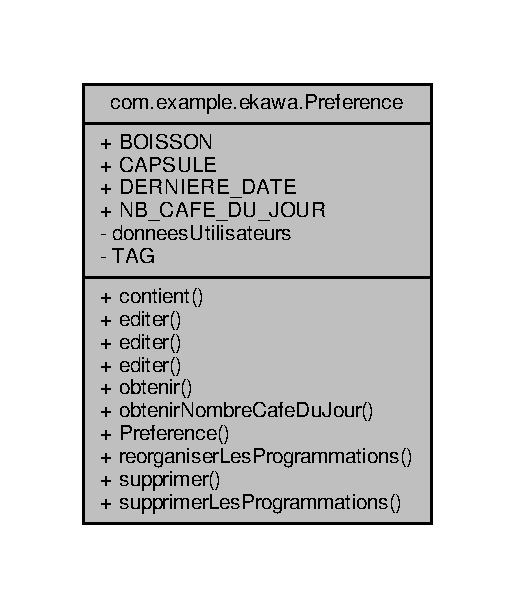
\includegraphics[width=247pt]{classcom_1_1example_1_1ekawa_1_1_preference__coll__graph}
\end{center}
\end{figure}
\subsubsection*{Fonctions membres publiques}
\begin{DoxyCompactItemize}
\item 
boolean \hyperlink{classcom_1_1example_1_1ekawa_1_1_preference_a25b7a4cfcc9fe5f9258471ce454a718a}{contient} (String nom\+Preference)
\begin{DoxyCompactList}\small\item\em Méthode qui permet de vérifer la présance d\textquotesingle{}une préférence. \end{DoxyCompactList}\item 
void \hyperlink{classcom_1_1example_1_1ekawa_1_1_preference_a5af7a0595acfd41f1bd0b34ca0bfcb2a}{editer} (String nom\+Preference, String valeur)
\begin{DoxyCompactList}\small\item\em Méthode qui permet de créer ou modifier une préférence. \end{DoxyCompactList}\item 
void \hyperlink{classcom_1_1example_1_1ekawa_1_1_preference_a7c14e4d338ffca5c03fda6b16289d8ce}{editer} (String nom\+Preference, int valeur)
\begin{DoxyCompactList}\small\item\em Méthode qui permet de créer ou modifier une préférence. \end{DoxyCompactList}\item 
void \hyperlink{classcom_1_1example_1_1ekawa_1_1_preference_a701dc293c4474f59028733e94b49b9da}{editer} (String nom\+Preference, boolean valeur)
\begin{DoxyCompactList}\small\item\em Méthode qui permet de créer ou modifier une préférence. \end{DoxyCompactList}\item 
Object \hyperlink{classcom_1_1example_1_1ekawa_1_1_preference_a485d7fe31708aa1b85c0e2dcdcc05c0d}{obtenir} (String nom\+Preference)
\begin{DoxyCompactList}\small\item\em Méthode qui permet d\textquotesingle{}obtenir une préférence. \end{DoxyCompactList}\item 
int \hyperlink{classcom_1_1example_1_1ekawa_1_1_preference_a5a8f4c9f845924a0ebb3aec5ca99a5f5}{obtenir\+Nombre\+Cafe\+Du\+Jour} (String date, int nombre\+Cafe\+Du\+Jour)
\item 
\hyperlink{classcom_1_1example_1_1ekawa_1_1_preference_a2594deda470fb764d1ac8e06cf504411}{Preference} (\hyperlink{classcom_1_1example_1_1ekawa_1_1_ihm}{Ihm} ihm)
\begin{DoxyCompactList}\small\item\em Constructeur de la classe \hyperlink{classcom_1_1example_1_1ekawa_1_1_preference}{Preference}. \end{DoxyCompactList}\item 
void \hyperlink{classcom_1_1example_1_1ekawa_1_1_preference_a98ab818534d930d51fa09de962780fe3}{reorganiser\+Les\+Programmations} (int position)
\begin{DoxyCompactList}\small\item\em Méthode qui permet de réorganiser les programmations. \end{DoxyCompactList}\item 
void \hyperlink{classcom_1_1example_1_1ekawa_1_1_preference_a63914421a8e7b8f79822853e3aff3106}{supprimer} (String nom\+Preference)
\begin{DoxyCompactList}\small\item\em Méthode qui permet de suprimer une préférence. \end{DoxyCompactList}\item 
void \hyperlink{classcom_1_1example_1_1ekawa_1_1_preference_aec0e98bb3cfb4d104c5c86a4259c56b5}{supprimer\+Les\+Programmations} ()
\begin{DoxyCompactList}\small\item\em Méthode qui permet de suprimer toutes les programmations. \end{DoxyCompactList}\end{DoxyCompactItemize}
\subsubsection*{Attributs publics statiques}
\begin{DoxyCompactItemize}
\item 
static final String \hyperlink{classcom_1_1example_1_1ekawa_1_1_preference_a6923224bd12c5b50259e5f376ed58a35}{B\+O\+I\+S\+S\+ON} = \char`\"{}boisson\+Preferee\char`\"{}
\item 
static final String \hyperlink{classcom_1_1example_1_1ekawa_1_1_preference_a64416823eba6f35e817636b31cb12265}{C\+A\+P\+S\+U\+LE} = \char`\"{}capsule\+Preferee\char`\"{}
\item 
static final String \hyperlink{classcom_1_1example_1_1ekawa_1_1_preference_a70095b2dd8748ba4bae554ff09d75d52}{D\+E\+R\+N\+I\+E\+R\+E\+\_\+\+D\+A\+TE} = \char`\"{}derniere\+Date\char`\"{}
\item 
static final String \hyperlink{classcom_1_1example_1_1ekawa_1_1_preference_a75bf6df7d252d793f34494240571a9ee}{N\+B\+\_\+\+C\+A\+F\+E\+\_\+\+D\+U\+\_\+\+J\+O\+UR} = \char`\"{}nombre\+Cafe\+Du\+Jour\char`\"{}
\end{DoxyCompactItemize}
\subsubsection*{Attributs privés}
\begin{DoxyCompactItemize}
\item 
Shared\+Preferences \hyperlink{classcom_1_1example_1_1ekawa_1_1_preference_a5ac49439bd1c8c3ff12dd9eb2475b894}{donnees\+Utilisateurs}
\end{DoxyCompactItemize}
\subsubsection*{Attributs privés statiques}
\begin{DoxyCompactItemize}
\item 
static final String \hyperlink{classcom_1_1example_1_1ekawa_1_1_preference_aeb5e1e787153c37929839622ac5d0339}{T\+AG} = \char`\"{}Preference\char`\"{}
\begin{DoxyCompactList}\small\item\em T\+AG pour les logs. \end{DoxyCompactList}\end{DoxyCompactItemize}


\subsubsection{Description détaillée}
Définit les caractéristiques des préfences de l\textquotesingle{}utilisateur d\textquotesingle{}E\+K\+A\+WA. 

Définition à la ligne \hyperlink{_preference_8java_source_l00023}{23} du fichier \hyperlink{_preference_8java_source}{Preference.\+java}.



\subsubsection{Documentation des constructeurs et destructeur}
\mbox{\Hypertarget{classcom_1_1example_1_1ekawa_1_1_preference_a2594deda470fb764d1ac8e06cf504411}\label{classcom_1_1example_1_1ekawa_1_1_preference_a2594deda470fb764d1ac8e06cf504411}} 
\index{com\+::example\+::ekawa\+::\+Preference@{com\+::example\+::ekawa\+::\+Preference}!Preference@{Preference}}
\index{Preference@{Preference}!com\+::example\+::ekawa\+::\+Preference@{com\+::example\+::ekawa\+::\+Preference}}
\paragraph{\texorpdfstring{Preference()}{Preference()}}
{\footnotesize\ttfamily com.\+example.\+ekawa.\+Preference.\+Preference (\begin{DoxyParamCaption}\item[{\hyperlink{classcom_1_1example_1_1ekawa_1_1_ihm}{Ihm}}]{ihm }\end{DoxyParamCaption})}



Constructeur de la classe \hyperlink{classcom_1_1example_1_1ekawa_1_1_preference}{Preference}. 



Définition à la ligne \hyperlink{_preference_8java_source_l00041}{41} du fichier \hyperlink{_preference_8java_source}{Preference.\+java}.


\begin{DoxyCode}
00042     \{
00043         Log.d(\hyperlink{classcom_1_1example_1_1ekawa_1_1_preference_aeb5e1e787153c37929839622ac5d0339}{TAG}, \textcolor{stringliteral}{"Preference()"});
00044         \hyperlink{classcom_1_1example_1_1ekawa_1_1_preference_a5ac49439bd1c8c3ff12dd9eb2475b894}{donneesUtilisateurs} = ihm.getPreferences(ihm.MODE\_PRIVATE);
00045     \}
\end{DoxyCode}


\subsubsection{Documentation des fonctions membres}
\mbox{\Hypertarget{classcom_1_1example_1_1ekawa_1_1_preference_a25b7a4cfcc9fe5f9258471ce454a718a}\label{classcom_1_1example_1_1ekawa_1_1_preference_a25b7a4cfcc9fe5f9258471ce454a718a}} 
\index{com\+::example\+::ekawa\+::\+Preference@{com\+::example\+::ekawa\+::\+Preference}!contient@{contient}}
\index{contient@{contient}!com\+::example\+::ekawa\+::\+Preference@{com\+::example\+::ekawa\+::\+Preference}}
\paragraph{\texorpdfstring{contient()}{contient()}}
{\footnotesize\ttfamily boolean com.\+example.\+ekawa.\+Preference.\+contient (\begin{DoxyParamCaption}\item[{String}]{nom\+Preference }\end{DoxyParamCaption})}



Méthode qui permet de vérifer la présance d\textquotesingle{}une préférence. 


\begin{DoxyParams}{Paramètres}
{\em nom\+Preference} & le nom de la préférence \\
\hline
\end{DoxyParams}
\begin{DoxyReturn}{Renvoie}
boolean la présance de la préférence 
\end{DoxyReturn}


Définition à la ligne \hyperlink{_preference_8java_source_l00087}{87} du fichier \hyperlink{_preference_8java_source}{Preference.\+java}.



Référencé par \hyperlink{_cafetiere_8java_source_l00731}{com.\+example.\+ekawa.\+Cafetiere.\+creer\+Une\+Programmation()}, \hyperlink{_cafetiere_8java_source_l00692}{com.\+example.\+ekawa.\+Cafetiere.\+initialiser\+Programmations()}, \hyperlink{_preference_8java_source_l00052}{com.\+example.\+ekawa.\+Preference.\+obtenir()}, \hyperlink{_preference_8java_source_l00063}{com.\+example.\+ekawa.\+Preference.\+obtenir\+Nombre\+Cafe\+Du\+Jour()}, \hyperlink{_preference_8java_source_l00157}{com.\+example.\+ekawa.\+Preference.\+reorganiser\+Les\+Programmations()}, et \hyperlink{_preference_8java_source_l00142}{com.\+example.\+ekawa.\+Preference.\+supprimer\+Les\+Programmations()}.


\begin{DoxyCode}
00088     \{
00089         Log.d(\hyperlink{classcom_1_1example_1_1ekawa_1_1_preference_aeb5e1e787153c37929839622ac5d0339}{TAG}, \textcolor{stringliteral}{"contient()"});
00090         \textcolor{keywordflow}{if}(\hyperlink{classcom_1_1example_1_1ekawa_1_1_preference_a5ac49439bd1c8c3ff12dd9eb2475b894}{donneesUtilisateurs}.contains(nomPreference))
00091             \textcolor{keywordflow}{return} \textcolor{keyword}{true};
00092         \textcolor{keywordflow}{return} \textcolor{keyword}{false};
00093     \}
\end{DoxyCode}
\mbox{\Hypertarget{classcom_1_1example_1_1ekawa_1_1_preference_a5af7a0595acfd41f1bd0b34ca0bfcb2a}\label{classcom_1_1example_1_1ekawa_1_1_preference_a5af7a0595acfd41f1bd0b34ca0bfcb2a}} 
\index{com\+::example\+::ekawa\+::\+Preference@{com\+::example\+::ekawa\+::\+Preference}!editer@{editer}}
\index{editer@{editer}!com\+::example\+::ekawa\+::\+Preference@{com\+::example\+::ekawa\+::\+Preference}}
\paragraph{\texorpdfstring{editer()}{editer()}\hspace{0.1cm}{\footnotesize\ttfamily [1/3]}}
{\footnotesize\ttfamily void com.\+example.\+ekawa.\+Preference.\+editer (\begin{DoxyParamCaption}\item[{String}]{nom\+Preference,  }\item[{String}]{valeur }\end{DoxyParamCaption})}



Méthode qui permet de créer ou modifier une préférence. 


\begin{DoxyParams}{Paramètres}
{\em nom\+Preference} & le nom de la préférence \\
\hline
{\em valeur} & la valeur de la préférence \\
\hline
\end{DoxyParams}


Définition à la ligne \hyperlink{_preference_8java_source_l00100}{100} du fichier \hyperlink{_preference_8java_source}{Preference.\+java}.



Référencé par \hyperlink{_cafetiere_8java_source_l00224}{com.\+example.\+ekawa.\+Cafetiere.\+changer\+Boisson\+Actuelle()}, \hyperlink{_cafetiere_8java_source_l00212}{com.\+example.\+ekawa.\+Cafetiere.\+changer\+Capsule\+Actuelle()}, \hyperlink{_cafetiere_8java_source_l00731}{com.\+example.\+ekawa.\+Cafetiere.\+creer\+Une\+Programmation()}, \hyperlink{_cafetiere_8java_source_l00527}{com.\+example.\+ekawa.\+Cafetiere.\+lancer\+Preparation\+Cafe()}, \hyperlink{_cafetiere_8java_source_l00775}{com.\+example.\+ekawa.\+Cafetiere.\+modifier\+Une\+Programmation()}, \hyperlink{_preference_8java_source_l00063}{com.\+example.\+ekawa.\+Preference.\+obtenir\+Nombre\+Cafe\+Du\+Jour()}, et \hyperlink{_preference_8java_source_l00157}{com.\+example.\+ekawa.\+Preference.\+reorganiser\+Les\+Programmations()}.


\begin{DoxyCode}
00101     \{
00102         Log.d(\hyperlink{classcom_1_1example_1_1ekawa_1_1_preference_aeb5e1e787153c37929839622ac5d0339}{TAG}, \textcolor{stringliteral}{"editer(String)"});
00103         \hyperlink{classcom_1_1example_1_1ekawa_1_1_preference_a5ac49439bd1c8c3ff12dd9eb2475b894}{donneesUtilisateurs}.edit().putString(nomPreference, valeur).apply();
00104     \}
\end{DoxyCode}
\mbox{\Hypertarget{classcom_1_1example_1_1ekawa_1_1_preference_a7c14e4d338ffca5c03fda6b16289d8ce}\label{classcom_1_1example_1_1ekawa_1_1_preference_a7c14e4d338ffca5c03fda6b16289d8ce}} 
\index{com\+::example\+::ekawa\+::\+Preference@{com\+::example\+::ekawa\+::\+Preference}!editer@{editer}}
\index{editer@{editer}!com\+::example\+::ekawa\+::\+Preference@{com\+::example\+::ekawa\+::\+Preference}}
\paragraph{\texorpdfstring{editer()}{editer()}\hspace{0.1cm}{\footnotesize\ttfamily [2/3]}}
{\footnotesize\ttfamily void com.\+example.\+ekawa.\+Preference.\+editer (\begin{DoxyParamCaption}\item[{String}]{nom\+Preference,  }\item[{int}]{valeur }\end{DoxyParamCaption})}



Méthode qui permet de créer ou modifier une préférence. 


\begin{DoxyParams}{Paramètres}
{\em nom\+Preference} & le nom de la préférence \\
\hline
{\em valeur} & la valeur de la préférence \\
\hline
\end{DoxyParams}


Définition à la ligne \hyperlink{_preference_8java_source_l00111}{111} du fichier \hyperlink{_preference_8java_source}{Preference.\+java}.


\begin{DoxyCode}
00112     \{
00113         Log.d(\hyperlink{classcom_1_1example_1_1ekawa_1_1_preference_aeb5e1e787153c37929839622ac5d0339}{TAG}, \textcolor{stringliteral}{"editer(int)"});
00114         \hyperlink{classcom_1_1example_1_1ekawa_1_1_preference_a5ac49439bd1c8c3ff12dd9eb2475b894}{donneesUtilisateurs}.edit().putInt(nomPreference, valeur).apply();
00115     \}
\end{DoxyCode}
\mbox{\Hypertarget{classcom_1_1example_1_1ekawa_1_1_preference_a701dc293c4474f59028733e94b49b9da}\label{classcom_1_1example_1_1ekawa_1_1_preference_a701dc293c4474f59028733e94b49b9da}} 
\index{com\+::example\+::ekawa\+::\+Preference@{com\+::example\+::ekawa\+::\+Preference}!editer@{editer}}
\index{editer@{editer}!com\+::example\+::ekawa\+::\+Preference@{com\+::example\+::ekawa\+::\+Preference}}
\paragraph{\texorpdfstring{editer()}{editer()}\hspace{0.1cm}{\footnotesize\ttfamily [3/3]}}
{\footnotesize\ttfamily void com.\+example.\+ekawa.\+Preference.\+editer (\begin{DoxyParamCaption}\item[{String}]{nom\+Preference,  }\item[{boolean}]{valeur }\end{DoxyParamCaption})}



Méthode qui permet de créer ou modifier une préférence. 


\begin{DoxyParams}{Paramètres}
{\em nom\+Preference} & le nom de la préférence \\
\hline
{\em valeur} & la valeur de la préférence \\
\hline
\end{DoxyParams}


Définition à la ligne \hyperlink{_preference_8java_source_l00122}{122} du fichier \hyperlink{_preference_8java_source}{Preference.\+java}.


\begin{DoxyCode}
00123     \{
00124         Log.d(\hyperlink{classcom_1_1example_1_1ekawa_1_1_preference_aeb5e1e787153c37929839622ac5d0339}{TAG}, \textcolor{stringliteral}{"editer(boolean)"});
00125         \hyperlink{classcom_1_1example_1_1ekawa_1_1_preference_a5ac49439bd1c8c3ff12dd9eb2475b894}{donneesUtilisateurs}.edit().putBoolean(nomPreference, valeur).apply();
00126     \}
\end{DoxyCode}
\mbox{\Hypertarget{classcom_1_1example_1_1ekawa_1_1_preference_a485d7fe31708aa1b85c0e2dcdcc05c0d}\label{classcom_1_1example_1_1ekawa_1_1_preference_a485d7fe31708aa1b85c0e2dcdcc05c0d}} 
\index{com\+::example\+::ekawa\+::\+Preference@{com\+::example\+::ekawa\+::\+Preference}!obtenir@{obtenir}}
\index{obtenir@{obtenir}!com\+::example\+::ekawa\+::\+Preference@{com\+::example\+::ekawa\+::\+Preference}}
\paragraph{\texorpdfstring{obtenir()}{obtenir()}}
{\footnotesize\ttfamily Object com.\+example.\+ekawa.\+Preference.\+obtenir (\begin{DoxyParamCaption}\item[{String}]{nom\+Preference }\end{DoxyParamCaption})}



Méthode qui permet d\textquotesingle{}obtenir une préférence. 


\begin{DoxyParams}{Paramètres}
{\em nom\+Preference} & le nom de la préférence \\
\hline
\end{DoxyParams}
\begin{DoxyReturn}{Renvoie}
Object la valeur de la préférence 
\end{DoxyReturn}


Définition à la ligne \hyperlink{_preference_8java_source_l00052}{52} du fichier \hyperlink{_preference_8java_source}{Preference.\+java}.



Références \hyperlink{_preference_8java_source_l00087}{com.\+example.\+ekawa.\+Preference.\+contient()}.



Référencé par \hyperlink{_cafetiere_8java_source_l00122}{com.\+example.\+ekawa.\+Cafetiere.\+initialiser\+Preference()}, \hyperlink{_cafetiere_8java_source_l00692}{com.\+example.\+ekawa.\+Cafetiere.\+initialiser\+Programmations()}, \hyperlink{_preference_8java_source_l00063}{com.\+example.\+ekawa.\+Preference.\+obtenir\+Nombre\+Cafe\+Du\+Jour()}, et \hyperlink{_preference_8java_source_l00157}{com.\+example.\+ekawa.\+Preference.\+reorganiser\+Les\+Programmations()}.


\begin{DoxyCode}
00053     \{
00054         Log.d(\hyperlink{classcom_1_1example_1_1ekawa_1_1_preference_aeb5e1e787153c37929839622ac5d0339}{TAG}, \textcolor{stringliteral}{"obtenir() nomPreference = "} + nomPreference);
00055         Map<String,?> donnees = \hyperlink{classcom_1_1example_1_1ekawa_1_1_preference_a5ac49439bd1c8c3ff12dd9eb2475b894}{donneesUtilisateurs}.getAll();
00056         Log.d(\hyperlink{classcom_1_1example_1_1ekawa_1_1_preference_aeb5e1e787153c37929839622ac5d0339}{TAG}, \textcolor{stringliteral}{"obtenir() donnees = "} + donnees);
00057         \textcolor{keywordflow}{if}(\hyperlink{classcom_1_1example_1_1ekawa_1_1_preference_a25b7a4cfcc9fe5f9258471ce454a718a}{contient}(nomPreference))
00058             \textcolor{keywordflow}{return} donnees.get(nomPreference);
00059         \textcolor{keywordflow}{else}
00060             \textcolor{keywordflow}{return} \textcolor{stringliteral}{""};
00061     \}
\end{DoxyCode}
\mbox{\Hypertarget{classcom_1_1example_1_1ekawa_1_1_preference_a5a8f4c9f845924a0ebb3aec5ca99a5f5}\label{classcom_1_1example_1_1ekawa_1_1_preference_a5a8f4c9f845924a0ebb3aec5ca99a5f5}} 
\index{com\+::example\+::ekawa\+::\+Preference@{com\+::example\+::ekawa\+::\+Preference}!obtenir\+Nombre\+Cafe\+Du\+Jour@{obtenir\+Nombre\+Cafe\+Du\+Jour}}
\index{obtenir\+Nombre\+Cafe\+Du\+Jour@{obtenir\+Nombre\+Cafe\+Du\+Jour}!com\+::example\+::ekawa\+::\+Preference@{com\+::example\+::ekawa\+::\+Preference}}
\paragraph{\texorpdfstring{obtenir\+Nombre\+Cafe\+Du\+Jour()}{obtenirNombreCafeDuJour()}}
{\footnotesize\ttfamily int com.\+example.\+ekawa.\+Preference.\+obtenir\+Nombre\+Cafe\+Du\+Jour (\begin{DoxyParamCaption}\item[{String}]{date,  }\item[{int}]{nombre\+Cafe\+Du\+Jour }\end{DoxyParamCaption})}



Définition à la ligne \hyperlink{_preference_8java_source_l00063}{63} du fichier \hyperlink{_preference_8java_source}{Preference.\+java}.



Références \hyperlink{_preference_8java_source_l00087}{com.\+example.\+ekawa.\+Preference.\+contient()}, \hyperlink{_preference_8java_source_l00033}{com.\+example.\+ekawa.\+Preference.\+D\+E\+R\+N\+I\+E\+R\+E\+\_\+\+D\+A\+TE}, \hyperlink{_preference_8java_source_l00100}{com.\+example.\+ekawa.\+Preference.\+editer()}, \hyperlink{_preference_8java_source_l00034}{com.\+example.\+ekawa.\+Preference.\+N\+B\+\_\+\+C\+A\+F\+E\+\_\+\+D\+U\+\_\+\+J\+O\+UR}, et \hyperlink{_preference_8java_source_l00052}{com.\+example.\+ekawa.\+Preference.\+obtenir()}.



Référencé par \hyperlink{_cafetiere_8java_source_l00122}{com.\+example.\+ekawa.\+Cafetiere.\+initialiser\+Preference()}.


\begin{DoxyCode}
00064     \{
00065         date = DateFormat.getDateInstance().format(\textcolor{keyword}{new} Date());
00066         \textcolor{keywordflow}{if}(!\hyperlink{classcom_1_1example_1_1ekawa_1_1_preference_a25b7a4cfcc9fe5f9258471ce454a718a}{contient}(\hyperlink{classcom_1_1example_1_1ekawa_1_1_preference_a2594deda470fb764d1ac8e06cf504411}{Preference}.DERNIERE\_DATE))
00067             \hyperlink{classcom_1_1example_1_1ekawa_1_1_preference_a5af7a0595acfd41f1bd0b34ca0bfcb2a}{editer}(\hyperlink{classcom_1_1example_1_1ekawa_1_1_preference_a2594deda470fb764d1ac8e06cf504411}{Preference}.DERNIERE\_DATE, date);
00068         \textcolor{keywordflow}{if}(!\hyperlink{classcom_1_1example_1_1ekawa_1_1_preference_a25b7a4cfcc9fe5f9258471ce454a718a}{contient}(\hyperlink{classcom_1_1example_1_1ekawa_1_1_preference_a2594deda470fb764d1ac8e06cf504411}{Preference}.NB\_CAFE\_DU\_JOUR))
00069             \hyperlink{classcom_1_1example_1_1ekawa_1_1_preference_a5af7a0595acfd41f1bd0b34ca0bfcb2a}{editer}(\hyperlink{classcom_1_1example_1_1ekawa_1_1_preference_a2594deda470fb764d1ac8e06cf504411}{Preference}.NB\_CAFE\_DU\_JOUR, nombreCafeDuJour);
00070 
00071         \textcolor{keywordflow}{if}(date.equals((String) \hyperlink{classcom_1_1example_1_1ekawa_1_1_preference_a485d7fe31708aa1b85c0e2dcdcc05c0d}{obtenir}(\hyperlink{classcom_1_1example_1_1ekawa_1_1_preference_a2594deda470fb764d1ac8e06cf504411}{Preference}.DERNIERE\_DATE)))
00072             nombreCafeDuJour = (\textcolor{keywordtype}{int}) \hyperlink{classcom_1_1example_1_1ekawa_1_1_preference_a485d7fe31708aa1b85c0e2dcdcc05c0d}{obtenir}(\hyperlink{classcom_1_1example_1_1ekawa_1_1_preference_a2594deda470fb764d1ac8e06cf504411}{Preference}.NB\_CAFE\_DU\_JOUR);
00073         \textcolor{keywordflow}{else}
00074         \{
00075             \hyperlink{classcom_1_1example_1_1ekawa_1_1_preference_a5af7a0595acfd41f1bd0b34ca0bfcb2a}{editer}(\hyperlink{classcom_1_1example_1_1ekawa_1_1_preference_a2594deda470fb764d1ac8e06cf504411}{Preference}.NB\_CAFE\_DU\_JOUR, nombreCafeDuJour);
00076             \hyperlink{classcom_1_1example_1_1ekawa_1_1_preference_a5af7a0595acfd41f1bd0b34ca0bfcb2a}{editer}(\hyperlink{classcom_1_1example_1_1ekawa_1_1_preference_a2594deda470fb764d1ac8e06cf504411}{Preference}.DERNIERE\_DATE, date);
00077             nombreCafeDuJour = 0;
00078         \}
00079         \textcolor{keywordflow}{return} nombreCafeDuJour;
00080     \}
\end{DoxyCode}
\mbox{\Hypertarget{classcom_1_1example_1_1ekawa_1_1_preference_a98ab818534d930d51fa09de962780fe3}\label{classcom_1_1example_1_1ekawa_1_1_preference_a98ab818534d930d51fa09de962780fe3}} 
\index{com\+::example\+::ekawa\+::\+Preference@{com\+::example\+::ekawa\+::\+Preference}!reorganiser\+Les\+Programmations@{reorganiser\+Les\+Programmations}}
\index{reorganiser\+Les\+Programmations@{reorganiser\+Les\+Programmations}!com\+::example\+::ekawa\+::\+Preference@{com\+::example\+::ekawa\+::\+Preference}}
\paragraph{\texorpdfstring{reorganiser\+Les\+Programmations()}{reorganiserLesProgrammations()}}
{\footnotesize\ttfamily void com.\+example.\+ekawa.\+Preference.\+reorganiser\+Les\+Programmations (\begin{DoxyParamCaption}\item[{int}]{position }\end{DoxyParamCaption})}



Méthode qui permet de réorganiser les programmations. 



Définition à la ligne \hyperlink{_preference_8java_source_l00157}{157} du fichier \hyperlink{_preference_8java_source}{Preference.\+java}.



Références \hyperlink{_programmation_8java_source_l00027}{com.\+example.\+ekawa.\+Programmation.\+B\+O\+I\+S\+S\+ON}, \hyperlink{_programmation_8java_source_l00026}{com.\+example.\+ekawa.\+Programmation.\+C\+A\+P\+S\+U\+LE}, \hyperlink{_preference_8java_source_l00087}{com.\+example.\+ekawa.\+Preference.\+contient()}, \hyperlink{_preference_8java_source_l00100}{com.\+example.\+ekawa.\+Preference.\+editer()}, \hyperlink{_programmation_8java_source_l00030}{com.\+example.\+ekawa.\+Programmation.\+F\+R\+E\+Q\+U\+E\+N\+CE}, \hyperlink{_programmation_8java_source_l00029}{com.\+example.\+ekawa.\+Programmation.\+H\+E\+U\+RE}, \hyperlink{_programmation_8java_source_l00025}{com.\+example.\+ekawa.\+Programmation.\+ID}, \hyperlink{_programmation_8java_source_l00028}{com.\+example.\+ekawa.\+Programmation.\+J\+O\+UR}, \hyperlink{_programmation_8java_source_l00023}{com.\+example.\+ekawa.\+Programmation.\+M\+A\+X\+\_\+\+P\+R\+O\+G\+R\+A\+M\+M\+A\+T\+I\+ON}, \hyperlink{_programmation_8java_source_l00022}{com.\+example.\+ekawa.\+Programmation.\+M\+I\+N\+\_\+\+P\+R\+O\+G\+R\+A\+M\+M\+A\+T\+I\+ON}, \hyperlink{_preference_8java_source_l00052}{com.\+example.\+ekawa.\+Preference.\+obtenir()}, \hyperlink{_preference_8java_source_l00132}{com.\+example.\+ekawa.\+Preference.\+supprimer()}, et \hyperlink{_programmation_8java_source_l00031}{com.\+example.\+ekawa.\+Programmation.\+T\+I\+C\+K\+ET}.



Référencé par \hyperlink{_cafetiere_8java_source_l00820}{com.\+example.\+ekawa.\+Cafetiere.\+supprimer\+Une\+Programmation()}.


\begin{DoxyCode}
00158     \{
00159         Log.d(\hyperlink{classcom_1_1example_1_1ekawa_1_1_preference_aeb5e1e787153c37929839622ac5d0339}{TAG}, \textcolor{stringliteral}{"reorganiserLesProgrammations()"});
00160         \textcolor{keywordflow}{if}(position >= Programmation.MIN\_PROGRAMMATION && position < Programmation.MAX\_PROGRAMMATION)
00161         \{
00162             \textcolor{keywordtype}{int} anciennePosition = position + 1;
00163             String idAncienneProgrammation = Programmation.ID + anciennePosition;
00164             String idNouvelleProgrammation = Programmation.ID + position;
00165             \textcolor{keywordflow}{if}(\hyperlink{classcom_1_1example_1_1ekawa_1_1_preference_a25b7a4cfcc9fe5f9258471ce454a718a}{contient}(idAncienneProgrammation))
00166             \{
00167                 \hyperlink{classcom_1_1example_1_1ekawa_1_1_preference_a5af7a0595acfd41f1bd0b34ca0bfcb2a}{editer}(idNouvelleProgrammation, (\textcolor{keywordtype}{int}) \hyperlink{classcom_1_1example_1_1ekawa_1_1_preference_a485d7fe31708aa1b85c0e2dcdcc05c0d}{obtenir}(idAncienneProgrammation));
00168                 \hyperlink{classcom_1_1example_1_1ekawa_1_1_preference_a5af7a0595acfd41f1bd0b34ca0bfcb2a}{editer}(idNouvelleProgrammation + \textcolor{stringliteral}{"\_"} + Programmation.CAPSULE, (\textcolor{keywordtype}{int}) 
      \hyperlink{classcom_1_1example_1_1ekawa_1_1_preference_a485d7fe31708aa1b85c0e2dcdcc05c0d}{obtenir}(idAncienneProgrammation + \textcolor{stringliteral}{"\_"} + Programmation.CAPSULE));
00169                 \hyperlink{classcom_1_1example_1_1ekawa_1_1_preference_a5af7a0595acfd41f1bd0b34ca0bfcb2a}{editer}(idNouvelleProgrammation + \textcolor{stringliteral}{"\_"} + Programmation.BOISSON, (\textcolor{keywordtype}{int}) 
      \hyperlink{classcom_1_1example_1_1ekawa_1_1_preference_a485d7fe31708aa1b85c0e2dcdcc05c0d}{obtenir}(idAncienneProgrammation + \textcolor{stringliteral}{"\_"} + Programmation.BOISSON));
00170                 \hyperlink{classcom_1_1example_1_1ekawa_1_1_preference_a5af7a0595acfd41f1bd0b34ca0bfcb2a}{editer}(idNouvelleProgrammation + \textcolor{stringliteral}{"\_"} + Programmation.JOUR, (\textcolor{keywordtype}{int}) 
      \hyperlink{classcom_1_1example_1_1ekawa_1_1_preference_a485d7fe31708aa1b85c0e2dcdcc05c0d}{obtenir}(idAncienneProgrammation + \textcolor{stringliteral}{"\_"} + Programmation.JOUR));
00171                 \hyperlink{classcom_1_1example_1_1ekawa_1_1_preference_a5af7a0595acfd41f1bd0b34ca0bfcb2a}{editer}(idNouvelleProgrammation + \textcolor{stringliteral}{"\_"} + Programmation.HEURE, (String) 
      \hyperlink{classcom_1_1example_1_1ekawa_1_1_preference_a485d7fe31708aa1b85c0e2dcdcc05c0d}{obtenir}(idAncienneProgrammation + \textcolor{stringliteral}{"\_"} + Programmation.HEURE));
00172                 \hyperlink{classcom_1_1example_1_1ekawa_1_1_preference_a5af7a0595acfd41f1bd0b34ca0bfcb2a}{editer}(idNouvelleProgrammation + \textcolor{stringliteral}{"\_"} + Programmation.FREQUENCE, (\textcolor{keywordtype}{int}) 
      \hyperlink{classcom_1_1example_1_1ekawa_1_1_preference_a485d7fe31708aa1b85c0e2dcdcc05c0d}{obtenir}(idAncienneProgrammation + \textcolor{stringliteral}{"\_"} + Programmation.FREQUENCE));
00173                 \hyperlink{classcom_1_1example_1_1ekawa_1_1_preference_a5af7a0595acfd41f1bd0b34ca0bfcb2a}{editer}(idNouvelleProgrammation + \textcolor{stringliteral}{"\_"} + Programmation.TICKET, (\textcolor{keywordtype}{int}) 
      \hyperlink{classcom_1_1example_1_1ekawa_1_1_preference_a485d7fe31708aa1b85c0e2dcdcc05c0d}{obtenir}(idAncienneProgrammation + \textcolor{stringliteral}{"\_"} + Programmation.TICKET));
00174 
00175                 \hyperlink{classcom_1_1example_1_1ekawa_1_1_preference_a63914421a8e7b8f79822853e3aff3106}{supprimer}(idAncienneProgrammation);
00176             \}
00177             \hyperlink{classcom_1_1example_1_1ekawa_1_1_preference_a98ab818534d930d51fa09de962780fe3}{reorganiserLesProgrammations}(anciennePosition);
00178         \}
00179     \}
\end{DoxyCode}
\mbox{\Hypertarget{classcom_1_1example_1_1ekawa_1_1_preference_a63914421a8e7b8f79822853e3aff3106}\label{classcom_1_1example_1_1ekawa_1_1_preference_a63914421a8e7b8f79822853e3aff3106}} 
\index{com\+::example\+::ekawa\+::\+Preference@{com\+::example\+::ekawa\+::\+Preference}!supprimer@{supprimer}}
\index{supprimer@{supprimer}!com\+::example\+::ekawa\+::\+Preference@{com\+::example\+::ekawa\+::\+Preference}}
\paragraph{\texorpdfstring{supprimer()}{supprimer()}}
{\footnotesize\ttfamily void com.\+example.\+ekawa.\+Preference.\+supprimer (\begin{DoxyParamCaption}\item[{String}]{nom\+Preference }\end{DoxyParamCaption})}



Méthode qui permet de suprimer une préférence. 


\begin{DoxyParams}{Paramètres}
{\em nom\+Preference} & le nom de la préférence \\
\hline
\end{DoxyParams}


Définition à la ligne \hyperlink{_preference_8java_source_l00132}{132} du fichier \hyperlink{_preference_8java_source}{Preference.\+java}.



Référencé par \hyperlink{_preference_8java_source_l00157}{com.\+example.\+ekawa.\+Preference.\+reorganiser\+Les\+Programmations()}, \hyperlink{_preference_8java_source_l00142}{com.\+example.\+ekawa.\+Preference.\+supprimer\+Les\+Programmations()}, et \hyperlink{_cafetiere_8java_source_l00820}{com.\+example.\+ekawa.\+Cafetiere.\+supprimer\+Une\+Programmation()}.


\begin{DoxyCode}
00133     \{
00134         Log.d(\hyperlink{classcom_1_1example_1_1ekawa_1_1_preference_aeb5e1e787153c37929839622ac5d0339}{TAG}, \textcolor{stringliteral}{"supprimer()"});
00135         \hyperlink{classcom_1_1example_1_1ekawa_1_1_preference_a5ac49439bd1c8c3ff12dd9eb2475b894}{donneesUtilisateurs}.edit().remove(nomPreference).apply();
00136     \}
\end{DoxyCode}
\mbox{\Hypertarget{classcom_1_1example_1_1ekawa_1_1_preference_aec0e98bb3cfb4d104c5c86a4259c56b5}\label{classcom_1_1example_1_1ekawa_1_1_preference_aec0e98bb3cfb4d104c5c86a4259c56b5}} 
\index{com\+::example\+::ekawa\+::\+Preference@{com\+::example\+::ekawa\+::\+Preference}!supprimer\+Les\+Programmations@{supprimer\+Les\+Programmations}}
\index{supprimer\+Les\+Programmations@{supprimer\+Les\+Programmations}!com\+::example\+::ekawa\+::\+Preference@{com\+::example\+::ekawa\+::\+Preference}}
\paragraph{\texorpdfstring{supprimer\+Les\+Programmations()}{supprimerLesProgrammations()}}
{\footnotesize\ttfamily void com.\+example.\+ekawa.\+Preference.\+supprimer\+Les\+Programmations (\begin{DoxyParamCaption}{ }\end{DoxyParamCaption})}



Méthode qui permet de suprimer toutes les programmations. 



Définition à la ligne \hyperlink{_preference_8java_source_l00142}{142} du fichier \hyperlink{_preference_8java_source}{Preference.\+java}.



Références \hyperlink{_preference_8java_source_l00087}{com.\+example.\+ekawa.\+Preference.\+contient()}, \hyperlink{_programmation_8java_source_l00025}{com.\+example.\+ekawa.\+Programmation.\+ID}, et \hyperlink{_preference_8java_source_l00132}{com.\+example.\+ekawa.\+Preference.\+supprimer()}.



Référencé par \hyperlink{_cafetiere_8java_source_l00834}{com.\+example.\+ekawa.\+Cafetiere.\+supprimer\+Les\+Programmations()}.


\begin{DoxyCode}
00143     \{
00144         Log.d(\hyperlink{classcom_1_1example_1_1ekawa_1_1_preference_aeb5e1e787153c37929839622ac5d0339}{TAG}, \textcolor{stringliteral}{"supprimerLesProgrammations()"});
00145         \textcolor{keywordtype}{int} \textcolor{keywordtype}{id} = 0;
00146         \textcolor{keywordflow}{while}(\hyperlink{classcom_1_1example_1_1ekawa_1_1_preference_a25b7a4cfcc9fe5f9258471ce454a718a}{contient}(Programmation.ID + \textcolor{keywordtype}{id}))
00147         \{
00148             String idProgrammation = Programmation.ID + id;
00149             \hyperlink{classcom_1_1example_1_1ekawa_1_1_preference_a63914421a8e7b8f79822853e3aff3106}{supprimer}(idProgrammation);
00150             ++id;
00151         \}
00152     \}
\end{DoxyCode}


\subsubsection{Documentation des données membres}
\mbox{\Hypertarget{classcom_1_1example_1_1ekawa_1_1_preference_a6923224bd12c5b50259e5f376ed58a35}\label{classcom_1_1example_1_1ekawa_1_1_preference_a6923224bd12c5b50259e5f376ed58a35}} 
\index{com\+::example\+::ekawa\+::\+Preference@{com\+::example\+::ekawa\+::\+Preference}!B\+O\+I\+S\+S\+ON@{B\+O\+I\+S\+S\+ON}}
\index{B\+O\+I\+S\+S\+ON@{B\+O\+I\+S\+S\+ON}!com\+::example\+::ekawa\+::\+Preference@{com\+::example\+::ekawa\+::\+Preference}}
\paragraph{\texorpdfstring{B\+O\+I\+S\+S\+ON}{BOISSON}}
{\footnotesize\ttfamily final String com.\+example.\+ekawa.\+Preference.\+B\+O\+I\+S\+S\+ON = \char`\"{}boisson\+Preferee\char`\"{}\hspace{0.3cm}{\ttfamily [static]}}



Définition à la ligne \hyperlink{_preference_8java_source_l00032}{32} du fichier \hyperlink{_preference_8java_source}{Preference.\+java}.



Référencé par \hyperlink{_cafetiere_8java_source_l00224}{com.\+example.\+ekawa.\+Cafetiere.\+changer\+Boisson\+Actuelle()}, et \hyperlink{_cafetiere_8java_source_l00122}{com.\+example.\+ekawa.\+Cafetiere.\+initialiser\+Preference()}.

\mbox{\Hypertarget{classcom_1_1example_1_1ekawa_1_1_preference_a64416823eba6f35e817636b31cb12265}\label{classcom_1_1example_1_1ekawa_1_1_preference_a64416823eba6f35e817636b31cb12265}} 
\index{com\+::example\+::ekawa\+::\+Preference@{com\+::example\+::ekawa\+::\+Preference}!C\+A\+P\+S\+U\+LE@{C\+A\+P\+S\+U\+LE}}
\index{C\+A\+P\+S\+U\+LE@{C\+A\+P\+S\+U\+LE}!com\+::example\+::ekawa\+::\+Preference@{com\+::example\+::ekawa\+::\+Preference}}
\paragraph{\texorpdfstring{C\+A\+P\+S\+U\+LE}{CAPSULE}}
{\footnotesize\ttfamily final String com.\+example.\+ekawa.\+Preference.\+C\+A\+P\+S\+U\+LE = \char`\"{}capsule\+Preferee\char`\"{}\hspace{0.3cm}{\ttfamily [static]}}



Définition à la ligne \hyperlink{_preference_8java_source_l00031}{31} du fichier \hyperlink{_preference_8java_source}{Preference.\+java}.



Référencé par \hyperlink{_cafetiere_8java_source_l00212}{com.\+example.\+ekawa.\+Cafetiere.\+changer\+Capsule\+Actuelle()}, et \hyperlink{_cafetiere_8java_source_l00122}{com.\+example.\+ekawa.\+Cafetiere.\+initialiser\+Preference()}.

\mbox{\Hypertarget{classcom_1_1example_1_1ekawa_1_1_preference_a70095b2dd8748ba4bae554ff09d75d52}\label{classcom_1_1example_1_1ekawa_1_1_preference_a70095b2dd8748ba4bae554ff09d75d52}} 
\index{com\+::example\+::ekawa\+::\+Preference@{com\+::example\+::ekawa\+::\+Preference}!D\+E\+R\+N\+I\+E\+R\+E\+\_\+\+D\+A\+TE@{D\+E\+R\+N\+I\+E\+R\+E\+\_\+\+D\+A\+TE}}
\index{D\+E\+R\+N\+I\+E\+R\+E\+\_\+\+D\+A\+TE@{D\+E\+R\+N\+I\+E\+R\+E\+\_\+\+D\+A\+TE}!com\+::example\+::ekawa\+::\+Preference@{com\+::example\+::ekawa\+::\+Preference}}
\paragraph{\texorpdfstring{D\+E\+R\+N\+I\+E\+R\+E\+\_\+\+D\+A\+TE}{DERNIERE\_DATE}}
{\footnotesize\ttfamily final String com.\+example.\+ekawa.\+Preference.\+D\+E\+R\+N\+I\+E\+R\+E\+\_\+\+D\+A\+TE = \char`\"{}derniere\+Date\char`\"{}\hspace{0.3cm}{\ttfamily [static]}}



Définition à la ligne \hyperlink{_preference_8java_source_l00033}{33} du fichier \hyperlink{_preference_8java_source}{Preference.\+java}.



Référencé par \hyperlink{_preference_8java_source_l00063}{com.\+example.\+ekawa.\+Preference.\+obtenir\+Nombre\+Cafe\+Du\+Jour()}.

\mbox{\Hypertarget{classcom_1_1example_1_1ekawa_1_1_preference_a5ac49439bd1c8c3ff12dd9eb2475b894}\label{classcom_1_1example_1_1ekawa_1_1_preference_a5ac49439bd1c8c3ff12dd9eb2475b894}} 
\index{com\+::example\+::ekawa\+::\+Preference@{com\+::example\+::ekawa\+::\+Preference}!donnees\+Utilisateurs@{donnees\+Utilisateurs}}
\index{donnees\+Utilisateurs@{donnees\+Utilisateurs}!com\+::example\+::ekawa\+::\+Preference@{com\+::example\+::ekawa\+::\+Preference}}
\paragraph{\texorpdfstring{donnees\+Utilisateurs}{donneesUtilisateurs}}
{\footnotesize\ttfamily Shared\+Preferences com.\+example.\+ekawa.\+Preference.\+donnees\+Utilisateurs\hspace{0.3cm}{\ttfamily [private]}}



Définition à la ligne \hyperlink{_preference_8java_source_l00036}{36} du fichier \hyperlink{_preference_8java_source}{Preference.\+java}.

\mbox{\Hypertarget{classcom_1_1example_1_1ekawa_1_1_preference_a75bf6df7d252d793f34494240571a9ee}\label{classcom_1_1example_1_1ekawa_1_1_preference_a75bf6df7d252d793f34494240571a9ee}} 
\index{com\+::example\+::ekawa\+::\+Preference@{com\+::example\+::ekawa\+::\+Preference}!N\+B\+\_\+\+C\+A\+F\+E\+\_\+\+D\+U\+\_\+\+J\+O\+UR@{N\+B\+\_\+\+C\+A\+F\+E\+\_\+\+D\+U\+\_\+\+J\+O\+UR}}
\index{N\+B\+\_\+\+C\+A\+F\+E\+\_\+\+D\+U\+\_\+\+J\+O\+UR@{N\+B\+\_\+\+C\+A\+F\+E\+\_\+\+D\+U\+\_\+\+J\+O\+UR}!com\+::example\+::ekawa\+::\+Preference@{com\+::example\+::ekawa\+::\+Preference}}
\paragraph{\texorpdfstring{N\+B\+\_\+\+C\+A\+F\+E\+\_\+\+D\+U\+\_\+\+J\+O\+UR}{NB\_CAFE\_DU\_JOUR}}
{\footnotesize\ttfamily final String com.\+example.\+ekawa.\+Preference.\+N\+B\+\_\+\+C\+A\+F\+E\+\_\+\+D\+U\+\_\+\+J\+O\+UR = \char`\"{}nombre\+Cafe\+Du\+Jour\char`\"{}\hspace{0.3cm}{\ttfamily [static]}}



Définition à la ligne \hyperlink{_preference_8java_source_l00034}{34} du fichier \hyperlink{_preference_8java_source}{Preference.\+java}.



Référencé par \hyperlink{_cafetiere_8java_source_l00527}{com.\+example.\+ekawa.\+Cafetiere.\+lancer\+Preparation\+Cafe()}, et \hyperlink{_preference_8java_source_l00063}{com.\+example.\+ekawa.\+Preference.\+obtenir\+Nombre\+Cafe\+Du\+Jour()}.

\mbox{\Hypertarget{classcom_1_1example_1_1ekawa_1_1_preference_aeb5e1e787153c37929839622ac5d0339}\label{classcom_1_1example_1_1ekawa_1_1_preference_aeb5e1e787153c37929839622ac5d0339}} 
\index{com\+::example\+::ekawa\+::\+Preference@{com\+::example\+::ekawa\+::\+Preference}!T\+AG@{T\+AG}}
\index{T\+AG@{T\+AG}!com\+::example\+::ekawa\+::\+Preference@{com\+::example\+::ekawa\+::\+Preference}}
\paragraph{\texorpdfstring{T\+AG}{TAG}}
{\footnotesize\ttfamily final String com.\+example.\+ekawa.\+Preference.\+T\+AG = \char`\"{}Preference\char`\"{}\hspace{0.3cm}{\ttfamily [static]}, {\ttfamily [private]}}



T\+AG pour les logs. 

Constantes 

Définition à la ligne \hyperlink{_preference_8java_source_l00028}{28} du fichier \hyperlink{_preference_8java_source}{Preference.\+java}.



La documentation de cette classe a été générée à partir du fichier suivant \+:\begin{DoxyCompactItemize}
\item 
\hyperlink{_preference_8java}{Preference.\+java}\end{DoxyCompactItemize}

\hypertarget{classcom_1_1example_1_1ekawa_1_1_programmation}{}\subsection{Référence de la classe com.\+example.\+ekawa.\+Programmation}
\label{classcom_1_1example_1_1ekawa_1_1_programmation}\index{com.\+example.\+ekawa.\+Programmation@{com.\+example.\+ekawa.\+Programmation}}


Définit les caractéristiques des programmations E\+K\+A\+WA.  




Graphe de collaboration de com.\+example.\+ekawa.\+Programmation\+:\nopagebreak
\begin{figure}[H]
\begin{center}
\leavevmode
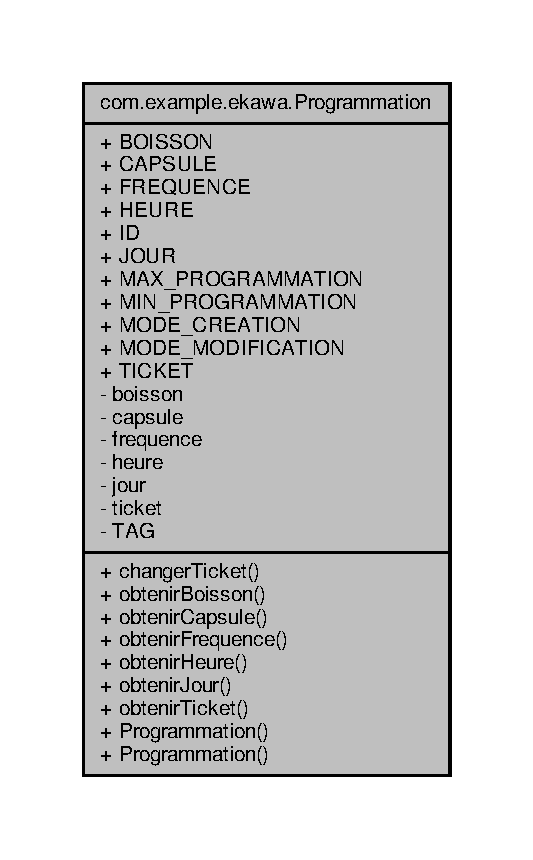
\includegraphics[width=256pt]{classcom_1_1example_1_1ekawa_1_1_programmation__coll__graph}
\end{center}
\end{figure}
\subsubsection*{Classes}
\begin{DoxyCompactItemize}
\item 
class \hyperlink{classcom_1_1example_1_1ekawa_1_1_programmation_1_1_frequences}{Frequences}
\item 
class \hyperlink{classcom_1_1example_1_1ekawa_1_1_programmation_1_1_jours}{Jours}
\end{DoxyCompactItemize}
\subsubsection*{Fonctions membres publiques}
\begin{DoxyCompactItemize}
\item 
void \hyperlink{classcom_1_1example_1_1ekawa_1_1_programmation_afb82bed29c60248fe8d966af8d6da897}{changer\+Ticket} (int \hyperlink{classcom_1_1example_1_1ekawa_1_1_programmation_a54ce49550025f7f5e5080f0548b08653}{ticket})
\begin{DoxyCompactList}\small\item\em Méthode qui permet de changer le ticket de la programmation. \end{DoxyCompactList}\item 
int \hyperlink{classcom_1_1example_1_1ekawa_1_1_programmation_a325b9fb3bb7e041e783ecc0ed8234c20}{obtenir\+Boisson} ()
\begin{DoxyCompactList}\small\item\em Méthode qui renvoie la boisson de la programmation. \end{DoxyCompactList}\item 
int \hyperlink{classcom_1_1example_1_1ekawa_1_1_programmation_a48d39b49a1250bbfaf51e4c32e934da0}{obtenir\+Capsule} ()
\begin{DoxyCompactList}\small\item\em Méthode qui renvoie la capsule de la programmation. \end{DoxyCompactList}\item 
int \hyperlink{classcom_1_1example_1_1ekawa_1_1_programmation_aa23acaed287ef27f86aec2771714a15f}{obtenir\+Frequence} ()
\begin{DoxyCompactList}\small\item\em Méthode qui renvoie la fréquence de la programmation. \end{DoxyCompactList}\item 
String \hyperlink{classcom_1_1example_1_1ekawa_1_1_programmation_ad8930be27ca5d1eed33c5e6729735897}{obtenir\+Heure} ()
\begin{DoxyCompactList}\small\item\em Méthode qui renvoie l\textquotesingle{}heure de la programmation. \end{DoxyCompactList}\item 
int \hyperlink{classcom_1_1example_1_1ekawa_1_1_programmation_a0e5090c0968474d6887518b7ef659337}{obtenir\+Jour} ()
\begin{DoxyCompactList}\small\item\em Méthode qui renvoie le jour de la programmation. \end{DoxyCompactList}\item 
int \hyperlink{classcom_1_1example_1_1ekawa_1_1_programmation_a63e8701af99c5bd974e028ba53209887}{obtenir\+Ticket} ()
\begin{DoxyCompactList}\small\item\em Méthode qui renvoie le ticket de la programmation. \end{DoxyCompactList}\item 
\hyperlink{classcom_1_1example_1_1ekawa_1_1_programmation_a9119f0bd9f104d0fbccdff1ab1f0eb64}{Programmation} (int \hyperlink{classcom_1_1example_1_1ekawa_1_1_programmation_a97573a66f9b2821a7445c69f346a5298}{capsule}, int \hyperlink{classcom_1_1example_1_1ekawa_1_1_programmation_a625a85ed4d0b16f52382fd458e0e5657}{boisson}, int \hyperlink{classcom_1_1example_1_1ekawa_1_1_programmation_a96605063cb4177fa382b1ce2388f544f}{jour}, String \hyperlink{classcom_1_1example_1_1ekawa_1_1_programmation_abfff674f6cd5f76ea4b8c37e8c558ffa}{heure}, int \hyperlink{classcom_1_1example_1_1ekawa_1_1_programmation_a6d0fd682b51727025ed8c4bf35fc8980}{frequence})
\begin{DoxyCompactList}\small\item\em Constructeur de la classe Cafetière. \end{DoxyCompactList}\item 
\hyperlink{classcom_1_1example_1_1ekawa_1_1_programmation_a06d8594e85da1735683f35228e7e6f8d}{Programmation} (int \hyperlink{classcom_1_1example_1_1ekawa_1_1_programmation_a97573a66f9b2821a7445c69f346a5298}{capsule}, int \hyperlink{classcom_1_1example_1_1ekawa_1_1_programmation_a625a85ed4d0b16f52382fd458e0e5657}{boisson}, int \hyperlink{classcom_1_1example_1_1ekawa_1_1_programmation_a96605063cb4177fa382b1ce2388f544f}{jour}, String \hyperlink{classcom_1_1example_1_1ekawa_1_1_programmation_abfff674f6cd5f76ea4b8c37e8c558ffa}{heure}, int \hyperlink{classcom_1_1example_1_1ekawa_1_1_programmation_a6d0fd682b51727025ed8c4bf35fc8980}{frequence}, int \hyperlink{classcom_1_1example_1_1ekawa_1_1_programmation_a54ce49550025f7f5e5080f0548b08653}{ticket})
\begin{DoxyCompactList}\small\item\em Constructeur de la classe Cafetière. \end{DoxyCompactList}\end{DoxyCompactItemize}
\subsubsection*{Attributs publics statiques}
\begin{DoxyCompactItemize}
\item 
static final String \hyperlink{classcom_1_1example_1_1ekawa_1_1_programmation_a87e9e78f01480283f2d4fa9f14443034}{B\+O\+I\+S\+S\+ON} = \char`\"{}boisson\char`\"{}
\item 
static final String \hyperlink{classcom_1_1example_1_1ekawa_1_1_programmation_a44b5687d27784aed685c77cf79d419fd}{C\+A\+P\+S\+U\+LE} = \char`\"{}capsule\char`\"{}
\item 
static final String \hyperlink{classcom_1_1example_1_1ekawa_1_1_programmation_aa5b1e7bbc58f4fef972e733498781a8e}{F\+R\+E\+Q\+U\+E\+N\+CE} = \char`\"{}frequence\char`\"{}
\item 
static final String \hyperlink{classcom_1_1example_1_1ekawa_1_1_programmation_aafa433ee13f4473d27cd7db34bbc4584}{H\+E\+U\+RE} = \char`\"{}heure\char`\"{}
\item 
static final String \hyperlink{classcom_1_1example_1_1ekawa_1_1_programmation_ae0552520e4ca9dc152bb503a7a00bf3a}{ID} = \char`\"{}programmation\char`\"{}
\item 
static final String \hyperlink{classcom_1_1example_1_1ekawa_1_1_programmation_a6ec3fe1846e45e6c0794eebdffeaf54b}{J\+O\+UR} = \char`\"{}jour\char`\"{}
\item 
static final int \hyperlink{classcom_1_1example_1_1ekawa_1_1_programmation_a056f8e2549c22393882b7306223a64c2}{M\+A\+X\+\_\+\+P\+R\+O\+G\+R\+A\+M\+M\+A\+T\+I\+ON} = 4
\item 
static final int \hyperlink{classcom_1_1example_1_1ekawa_1_1_programmation_a1167f22eb96c9c94bfc407aa3e166237}{M\+I\+N\+\_\+\+P\+R\+O\+G\+R\+A\+M\+M\+A\+T\+I\+ON} = 0
\item 
static final boolean \hyperlink{classcom_1_1example_1_1ekawa_1_1_programmation_a79242eac5d971bdb23eaf4ab930f774d}{M\+O\+D\+E\+\_\+\+C\+R\+E\+A\+T\+I\+ON} = false
\item 
static final boolean \hyperlink{classcom_1_1example_1_1ekawa_1_1_programmation_a33fb0a465e66ba5854a07e3050c12c04}{M\+O\+D\+E\+\_\+\+M\+O\+D\+I\+F\+I\+C\+A\+T\+I\+ON} = true
\item 
static final String \hyperlink{classcom_1_1example_1_1ekawa_1_1_programmation_aa04b411478bfe88f8f53057dfca5c650}{T\+I\+C\+K\+ET} = \char`\"{}ticket\char`\"{}
\end{DoxyCompactItemize}
\subsubsection*{Attributs privés}
\begin{DoxyCompactItemize}
\item 
int \hyperlink{classcom_1_1example_1_1ekawa_1_1_programmation_a625a85ed4d0b16f52382fd458e0e5657}{boisson}
\item 
int \hyperlink{classcom_1_1example_1_1ekawa_1_1_programmation_a97573a66f9b2821a7445c69f346a5298}{capsule}
\item 
int \hyperlink{classcom_1_1example_1_1ekawa_1_1_programmation_a6d0fd682b51727025ed8c4bf35fc8980}{frequence}
\item 
String \hyperlink{classcom_1_1example_1_1ekawa_1_1_programmation_abfff674f6cd5f76ea4b8c37e8c558ffa}{heure}
\item 
int \hyperlink{classcom_1_1example_1_1ekawa_1_1_programmation_a96605063cb4177fa382b1ce2388f544f}{jour}
\item 
int \hyperlink{classcom_1_1example_1_1ekawa_1_1_programmation_a54ce49550025f7f5e5080f0548b08653}{ticket}
\end{DoxyCompactItemize}
\subsubsection*{Attributs privés statiques}
\begin{DoxyCompactItemize}
\item 
static final String \hyperlink{classcom_1_1example_1_1ekawa_1_1_programmation_a85d255c2386eb6751905a45dba634742}{T\+AG} = \char`\"{}Programmation\char`\"{}
\end{DoxyCompactItemize}


\subsubsection{Description détaillée}
Définit les caractéristiques des programmations E\+K\+A\+WA. 

Définition à la ligne \hyperlink{_programmation_8java_source_l00015}{15} du fichier \hyperlink{_programmation_8java_source}{Programmation.\+java}.



\subsubsection{Documentation des constructeurs et destructeur}
\mbox{\Hypertarget{classcom_1_1example_1_1ekawa_1_1_programmation_a9119f0bd9f104d0fbccdff1ab1f0eb64}\label{classcom_1_1example_1_1ekawa_1_1_programmation_a9119f0bd9f104d0fbccdff1ab1f0eb64}} 
\index{com\+::example\+::ekawa\+::\+Programmation@{com\+::example\+::ekawa\+::\+Programmation}!Programmation@{Programmation}}
\index{Programmation@{Programmation}!com\+::example\+::ekawa\+::\+Programmation@{com\+::example\+::ekawa\+::\+Programmation}}
\paragraph{\texorpdfstring{Programmation()}{Programmation()}\hspace{0.1cm}{\footnotesize\ttfamily [1/2]}}
{\footnotesize\ttfamily com.\+example.\+ekawa.\+Programmation.\+Programmation (\begin{DoxyParamCaption}\item[{int}]{capsule,  }\item[{int}]{boisson,  }\item[{int}]{jour,  }\item[{String}]{heure,  }\item[{int}]{frequence }\end{DoxyParamCaption})}



Constructeur de la classe Cafetière. 


\begin{DoxyParams}{Paramètres}
{\em capsule} & la capsule demandée \\
\hline
{\em boisson} & la boisson demandée \\
\hline
{\em jour} & le jour demandé \\
\hline
{\em heure} & l\textquotesingle{}heure demandée \\
\hline
{\em frequence} & la fréquence demandée \\
\hline
\end{DoxyParams}


Définition à la ligne \hyperlink{_programmation_8java_source_l00091}{91} du fichier \hyperlink{_programmation_8java_source}{Programmation.\+java}.



Références \hyperlink{_programmation_8java_source_l00077}{com.\+example.\+ekawa.\+Programmation.\+boisson}, \hyperlink{_programmation_8java_source_l00076}{com.\+example.\+ekawa.\+Programmation.\+capsule}, \hyperlink{_programmation_8java_source_l00080}{com.\+example.\+ekawa.\+Programmation.\+frequence}, \hyperlink{_programmation_8java_source_l00079}{com.\+example.\+ekawa.\+Programmation.\+heure}, et \hyperlink{_programmation_8java_source_l00078}{com.\+example.\+ekawa.\+Programmation.\+jour}.


\begin{DoxyCode}
00092     \{
00093         this.\hyperlink{classcom_1_1example_1_1ekawa_1_1_programmation_a97573a66f9b2821a7445c69f346a5298}{capsule} = \hyperlink{classcom_1_1example_1_1ekawa_1_1_programmation_a97573a66f9b2821a7445c69f346a5298}{capsule};
00094         this.\hyperlink{classcom_1_1example_1_1ekawa_1_1_programmation_a625a85ed4d0b16f52382fd458e0e5657}{boisson} = \hyperlink{classcom_1_1example_1_1ekawa_1_1_programmation_a625a85ed4d0b16f52382fd458e0e5657}{boisson};
00095         this.\hyperlink{classcom_1_1example_1_1ekawa_1_1_programmation_a96605063cb4177fa382b1ce2388f544f}{jour} = \hyperlink{classcom_1_1example_1_1ekawa_1_1_programmation_a96605063cb4177fa382b1ce2388f544f}{jour};
00096         this.\hyperlink{classcom_1_1example_1_1ekawa_1_1_programmation_abfff674f6cd5f76ea4b8c37e8c558ffa}{heure} = \hyperlink{classcom_1_1example_1_1ekawa_1_1_programmation_abfff674f6cd5f76ea4b8c37e8c558ffa}{heure};
00097         this.\hyperlink{classcom_1_1example_1_1ekawa_1_1_programmation_a6d0fd682b51727025ed8c4bf35fc8980}{frequence} = \hyperlink{classcom_1_1example_1_1ekawa_1_1_programmation_a6d0fd682b51727025ed8c4bf35fc8980}{frequence};
00098         this.\hyperlink{classcom_1_1example_1_1ekawa_1_1_programmation_a54ce49550025f7f5e5080f0548b08653}{ticket} = 0;
00099     \}
\end{DoxyCode}
\mbox{\Hypertarget{classcom_1_1example_1_1ekawa_1_1_programmation_a06d8594e85da1735683f35228e7e6f8d}\label{classcom_1_1example_1_1ekawa_1_1_programmation_a06d8594e85da1735683f35228e7e6f8d}} 
\index{com\+::example\+::ekawa\+::\+Programmation@{com\+::example\+::ekawa\+::\+Programmation}!Programmation@{Programmation}}
\index{Programmation@{Programmation}!com\+::example\+::ekawa\+::\+Programmation@{com\+::example\+::ekawa\+::\+Programmation}}
\paragraph{\texorpdfstring{Programmation()}{Programmation()}\hspace{0.1cm}{\footnotesize\ttfamily [2/2]}}
{\footnotesize\ttfamily com.\+example.\+ekawa.\+Programmation.\+Programmation (\begin{DoxyParamCaption}\item[{int}]{capsule,  }\item[{int}]{boisson,  }\item[{int}]{jour,  }\item[{String}]{heure,  }\item[{int}]{frequence,  }\item[{int}]{ticket }\end{DoxyParamCaption})}



Constructeur de la classe Cafetière. 


\begin{DoxyParams}{Paramètres}
{\em capsule} & la capsule demandée \\
\hline
{\em boisson} & la boisson demandée \\
\hline
{\em jour} & le jour demandé \\
\hline
{\em heure} & l\textquotesingle{}heure demandée \\
\hline
{\em frequence} & la fréquence demandée \\
\hline
{\em ticket} & le ticket de la programmation \\
\hline
\end{DoxyParams}


Définition à la ligne \hyperlink{_programmation_8java_source_l00110}{110} du fichier \hyperlink{_programmation_8java_source}{Programmation.\+java}.



Références \hyperlink{_programmation_8java_source_l00077}{com.\+example.\+ekawa.\+Programmation.\+boisson}, \hyperlink{_programmation_8java_source_l00076}{com.\+example.\+ekawa.\+Programmation.\+capsule}, \hyperlink{_programmation_8java_source_l00080}{com.\+example.\+ekawa.\+Programmation.\+frequence}, \hyperlink{_programmation_8java_source_l00079}{com.\+example.\+ekawa.\+Programmation.\+heure}, \hyperlink{_programmation_8java_source_l00078}{com.\+example.\+ekawa.\+Programmation.\+jour}, et \hyperlink{_programmation_8java_source_l00081}{com.\+example.\+ekawa.\+Programmation.\+ticket}.


\begin{DoxyCode}
00111     \{
00112         this.\hyperlink{classcom_1_1example_1_1ekawa_1_1_programmation_a97573a66f9b2821a7445c69f346a5298}{capsule} = \hyperlink{classcom_1_1example_1_1ekawa_1_1_programmation_a97573a66f9b2821a7445c69f346a5298}{capsule};
00113         this.\hyperlink{classcom_1_1example_1_1ekawa_1_1_programmation_a625a85ed4d0b16f52382fd458e0e5657}{boisson} = \hyperlink{classcom_1_1example_1_1ekawa_1_1_programmation_a625a85ed4d0b16f52382fd458e0e5657}{boisson};
00114         this.\hyperlink{classcom_1_1example_1_1ekawa_1_1_programmation_a96605063cb4177fa382b1ce2388f544f}{jour} = \hyperlink{classcom_1_1example_1_1ekawa_1_1_programmation_a96605063cb4177fa382b1ce2388f544f}{jour};
00115         this.\hyperlink{classcom_1_1example_1_1ekawa_1_1_programmation_abfff674f6cd5f76ea4b8c37e8c558ffa}{heure} = \hyperlink{classcom_1_1example_1_1ekawa_1_1_programmation_abfff674f6cd5f76ea4b8c37e8c558ffa}{heure};
00116         this.\hyperlink{classcom_1_1example_1_1ekawa_1_1_programmation_a6d0fd682b51727025ed8c4bf35fc8980}{frequence} = \hyperlink{classcom_1_1example_1_1ekawa_1_1_programmation_a6d0fd682b51727025ed8c4bf35fc8980}{frequence};
00117         this.\hyperlink{classcom_1_1example_1_1ekawa_1_1_programmation_a54ce49550025f7f5e5080f0548b08653}{ticket} = \hyperlink{classcom_1_1example_1_1ekawa_1_1_programmation_a54ce49550025f7f5e5080f0548b08653}{ticket};
00118     \}
\end{DoxyCode}


\subsubsection{Documentation des fonctions membres}
\mbox{\Hypertarget{classcom_1_1example_1_1ekawa_1_1_programmation_afb82bed29c60248fe8d966af8d6da897}\label{classcom_1_1example_1_1ekawa_1_1_programmation_afb82bed29c60248fe8d966af8d6da897}} 
\index{com\+::example\+::ekawa\+::\+Programmation@{com\+::example\+::ekawa\+::\+Programmation}!changer\+Ticket@{changer\+Ticket}}
\index{changer\+Ticket@{changer\+Ticket}!com\+::example\+::ekawa\+::\+Programmation@{com\+::example\+::ekawa\+::\+Programmation}}
\paragraph{\texorpdfstring{changer\+Ticket()}{changerTicket()}}
{\footnotesize\ttfamily void com.\+example.\+ekawa.\+Programmation.\+changer\+Ticket (\begin{DoxyParamCaption}\item[{int}]{ticket }\end{DoxyParamCaption})}



Méthode qui permet de changer le ticket de la programmation. 


\begin{DoxyParams}{Paramètres}
{\em ticket} & le ticket de la programmation \\
\hline
\end{DoxyParams}


Définition à la ligne \hyperlink{_programmation_8java_source_l00178}{178} du fichier \hyperlink{_programmation_8java_source}{Programmation.\+java}.



Références \hyperlink{_programmation_8java_source_l00081}{com.\+example.\+ekawa.\+Programmation.\+ticket}.



Référencé par \hyperlink{_cafetiere_8java_source_l00731}{com.\+example.\+ekawa.\+Cafetiere.\+creer\+Une\+Programmation()}.


\begin{DoxyCode}
00179     \{
00180         this.\hyperlink{classcom_1_1example_1_1ekawa_1_1_programmation_a54ce49550025f7f5e5080f0548b08653}{ticket} = \hyperlink{classcom_1_1example_1_1ekawa_1_1_programmation_a54ce49550025f7f5e5080f0548b08653}{ticket};
00181     \}
\end{DoxyCode}
\mbox{\Hypertarget{classcom_1_1example_1_1ekawa_1_1_programmation_a325b9fb3bb7e041e783ecc0ed8234c20}\label{classcom_1_1example_1_1ekawa_1_1_programmation_a325b9fb3bb7e041e783ecc0ed8234c20}} 
\index{com\+::example\+::ekawa\+::\+Programmation@{com\+::example\+::ekawa\+::\+Programmation}!obtenir\+Boisson@{obtenir\+Boisson}}
\index{obtenir\+Boisson@{obtenir\+Boisson}!com\+::example\+::ekawa\+::\+Programmation@{com\+::example\+::ekawa\+::\+Programmation}}
\paragraph{\texorpdfstring{obtenir\+Boisson()}{obtenirBoisson()}}
{\footnotesize\ttfamily int com.\+example.\+ekawa.\+Programmation.\+obtenir\+Boisson (\begin{DoxyParamCaption}{ }\end{DoxyParamCaption})}



Méthode qui renvoie la boisson de la programmation. 

\begin{DoxyReturn}{Renvoie}
int la boisson de la programmation 
\end{DoxyReturn}


Définition à la ligne \hyperlink{_programmation_8java_source_l00133}{133} du fichier \hyperlink{_programmation_8java_source}{Programmation.\+java}.



Références \hyperlink{_programmation_8java_source_l00077}{com.\+example.\+ekawa.\+Programmation.\+boisson}.



Référencé par \hyperlink{_cafetiere_8java_source_l00731}{com.\+example.\+ekawa.\+Cafetiere.\+creer\+Une\+Programmation()}, et \hyperlink{_ihm_8java_source_l00668}{com.\+example.\+ekawa.\+Ihm.\+initialiser\+Page\+Programmer()}.


\begin{DoxyCode}
00134     \{
00135         \textcolor{keywordflow}{return} \hyperlink{classcom_1_1example_1_1ekawa_1_1_programmation_a625a85ed4d0b16f52382fd458e0e5657}{boisson};
00136     \}
\end{DoxyCode}
\mbox{\Hypertarget{classcom_1_1example_1_1ekawa_1_1_programmation_a48d39b49a1250bbfaf51e4c32e934da0}\label{classcom_1_1example_1_1ekawa_1_1_programmation_a48d39b49a1250bbfaf51e4c32e934da0}} 
\index{com\+::example\+::ekawa\+::\+Programmation@{com\+::example\+::ekawa\+::\+Programmation}!obtenir\+Capsule@{obtenir\+Capsule}}
\index{obtenir\+Capsule@{obtenir\+Capsule}!com\+::example\+::ekawa\+::\+Programmation@{com\+::example\+::ekawa\+::\+Programmation}}
\paragraph{\texorpdfstring{obtenir\+Capsule()}{obtenirCapsule()}}
{\footnotesize\ttfamily int com.\+example.\+ekawa.\+Programmation.\+obtenir\+Capsule (\begin{DoxyParamCaption}{ }\end{DoxyParamCaption})}



Méthode qui renvoie la capsule de la programmation. 

\begin{DoxyReturn}{Renvoie}
int la capsule de la programmation 
\end{DoxyReturn}


Définition à la ligne \hyperlink{_programmation_8java_source_l00124}{124} du fichier \hyperlink{_programmation_8java_source}{Programmation.\+java}.



Références \hyperlink{_programmation_8java_source_l00076}{com.\+example.\+ekawa.\+Programmation.\+capsule}.



Référencé par \hyperlink{_cafetiere_8java_source_l00731}{com.\+example.\+ekawa.\+Cafetiere.\+creer\+Une\+Programmation()}, et \hyperlink{_ihm_8java_source_l00668}{com.\+example.\+ekawa.\+Ihm.\+initialiser\+Page\+Programmer()}.


\begin{DoxyCode}
00125     \{
00126         \textcolor{keywordflow}{return} \hyperlink{classcom_1_1example_1_1ekawa_1_1_programmation_a97573a66f9b2821a7445c69f346a5298}{capsule};
00127     \}
\end{DoxyCode}
\mbox{\Hypertarget{classcom_1_1example_1_1ekawa_1_1_programmation_aa23acaed287ef27f86aec2771714a15f}\label{classcom_1_1example_1_1ekawa_1_1_programmation_aa23acaed287ef27f86aec2771714a15f}} 
\index{com\+::example\+::ekawa\+::\+Programmation@{com\+::example\+::ekawa\+::\+Programmation}!obtenir\+Frequence@{obtenir\+Frequence}}
\index{obtenir\+Frequence@{obtenir\+Frequence}!com\+::example\+::ekawa\+::\+Programmation@{com\+::example\+::ekawa\+::\+Programmation}}
\paragraph{\texorpdfstring{obtenir\+Frequence()}{obtenirFrequence()}}
{\footnotesize\ttfamily int com.\+example.\+ekawa.\+Programmation.\+obtenir\+Frequence (\begin{DoxyParamCaption}{ }\end{DoxyParamCaption})}



Méthode qui renvoie la fréquence de la programmation. 

\begin{DoxyReturn}{Renvoie}
int la fréquence de la programmation 
\end{DoxyReturn}


Définition à la ligne \hyperlink{_programmation_8java_source_l00160}{160} du fichier \hyperlink{_programmation_8java_source}{Programmation.\+java}.



Références \hyperlink{_programmation_8java_source_l00080}{com.\+example.\+ekawa.\+Programmation.\+frequence}.



Référencé par \hyperlink{_cafetiere_8java_source_l00731}{com.\+example.\+ekawa.\+Cafetiere.\+creer\+Une\+Programmation()}, et \hyperlink{_ihm_8java_source_l00668}{com.\+example.\+ekawa.\+Ihm.\+initialiser\+Page\+Programmer()}.


\begin{DoxyCode}
00161     \{
00162         \textcolor{keywordflow}{return} \hyperlink{classcom_1_1example_1_1ekawa_1_1_programmation_a6d0fd682b51727025ed8c4bf35fc8980}{frequence};
00163     \}
\end{DoxyCode}
\mbox{\Hypertarget{classcom_1_1example_1_1ekawa_1_1_programmation_ad8930be27ca5d1eed33c5e6729735897}\label{classcom_1_1example_1_1ekawa_1_1_programmation_ad8930be27ca5d1eed33c5e6729735897}} 
\index{com\+::example\+::ekawa\+::\+Programmation@{com\+::example\+::ekawa\+::\+Programmation}!obtenir\+Heure@{obtenir\+Heure}}
\index{obtenir\+Heure@{obtenir\+Heure}!com\+::example\+::ekawa\+::\+Programmation@{com\+::example\+::ekawa\+::\+Programmation}}
\paragraph{\texorpdfstring{obtenir\+Heure()}{obtenirHeure()}}
{\footnotesize\ttfamily String com.\+example.\+ekawa.\+Programmation.\+obtenir\+Heure (\begin{DoxyParamCaption}{ }\end{DoxyParamCaption})}



Méthode qui renvoie l\textquotesingle{}heure de la programmation. 

\begin{DoxyReturn}{Renvoie}
int l\textquotesingle{}heure de la programmation 
\end{DoxyReturn}


Définition à la ligne \hyperlink{_programmation_8java_source_l00151}{151} du fichier \hyperlink{_programmation_8java_source}{Programmation.\+java}.



Références \hyperlink{_programmation_8java_source_l00079}{com.\+example.\+ekawa.\+Programmation.\+heure}.



Référencé par \hyperlink{_cafetiere_8java_source_l00731}{com.\+example.\+ekawa.\+Cafetiere.\+creer\+Une\+Programmation()}, et \hyperlink{_ihm_8java_source_l00668}{com.\+example.\+ekawa.\+Ihm.\+initialiser\+Page\+Programmer()}.


\begin{DoxyCode}
00152     \{
00153         \textcolor{keywordflow}{return} \hyperlink{classcom_1_1example_1_1ekawa_1_1_programmation_abfff674f6cd5f76ea4b8c37e8c558ffa}{heure};
00154     \}
\end{DoxyCode}
\mbox{\Hypertarget{classcom_1_1example_1_1ekawa_1_1_programmation_a0e5090c0968474d6887518b7ef659337}\label{classcom_1_1example_1_1ekawa_1_1_programmation_a0e5090c0968474d6887518b7ef659337}} 
\index{com\+::example\+::ekawa\+::\+Programmation@{com\+::example\+::ekawa\+::\+Programmation}!obtenir\+Jour@{obtenir\+Jour}}
\index{obtenir\+Jour@{obtenir\+Jour}!com\+::example\+::ekawa\+::\+Programmation@{com\+::example\+::ekawa\+::\+Programmation}}
\paragraph{\texorpdfstring{obtenir\+Jour()}{obtenirJour()}}
{\footnotesize\ttfamily int com.\+example.\+ekawa.\+Programmation.\+obtenir\+Jour (\begin{DoxyParamCaption}{ }\end{DoxyParamCaption})}



Méthode qui renvoie le jour de la programmation. 

\begin{DoxyReturn}{Renvoie}
int le jour de la programmation 
\end{DoxyReturn}


Définition à la ligne \hyperlink{_programmation_8java_source_l00142}{142} du fichier \hyperlink{_programmation_8java_source}{Programmation.\+java}.



Références \hyperlink{_programmation_8java_source_l00078}{com.\+example.\+ekawa.\+Programmation.\+jour}.



Référencé par \hyperlink{_cafetiere_8java_source_l00731}{com.\+example.\+ekawa.\+Cafetiere.\+creer\+Une\+Programmation()}, et \hyperlink{_ihm_8java_source_l00668}{com.\+example.\+ekawa.\+Ihm.\+initialiser\+Page\+Programmer()}.


\begin{DoxyCode}
00143     \{
00144         \textcolor{keywordflow}{return} \hyperlink{classcom_1_1example_1_1ekawa_1_1_programmation_a96605063cb4177fa382b1ce2388f544f}{jour};
00145     \}
\end{DoxyCode}
\mbox{\Hypertarget{classcom_1_1example_1_1ekawa_1_1_programmation_a63e8701af99c5bd974e028ba53209887}\label{classcom_1_1example_1_1ekawa_1_1_programmation_a63e8701af99c5bd974e028ba53209887}} 
\index{com\+::example\+::ekawa\+::\+Programmation@{com\+::example\+::ekawa\+::\+Programmation}!obtenir\+Ticket@{obtenir\+Ticket}}
\index{obtenir\+Ticket@{obtenir\+Ticket}!com\+::example\+::ekawa\+::\+Programmation@{com\+::example\+::ekawa\+::\+Programmation}}
\paragraph{\texorpdfstring{obtenir\+Ticket()}{obtenirTicket()}}
{\footnotesize\ttfamily int com.\+example.\+ekawa.\+Programmation.\+obtenir\+Ticket (\begin{DoxyParamCaption}{ }\end{DoxyParamCaption})}



Méthode qui renvoie le ticket de la programmation. 

\begin{DoxyReturn}{Renvoie}
int le ticket de la programmation 
\end{DoxyReturn}


Définition à la ligne \hyperlink{_programmation_8java_source_l00169}{169} du fichier \hyperlink{_programmation_8java_source}{Programmation.\+java}.



Références \hyperlink{_programmation_8java_source_l00081}{com.\+example.\+ekawa.\+Programmation.\+ticket}.



Référencé par \hyperlink{_cafetiere_8java_source_l00731}{com.\+example.\+ekawa.\+Cafetiere.\+creer\+Une\+Programmation()}.


\begin{DoxyCode}
00170     \{
00171         \textcolor{keywordflow}{return} \hyperlink{classcom_1_1example_1_1ekawa_1_1_programmation_a54ce49550025f7f5e5080f0548b08653}{ticket};
00172     \}
\end{DoxyCode}


\subsubsection{Documentation des données membres}
\mbox{\Hypertarget{classcom_1_1example_1_1ekawa_1_1_programmation_a87e9e78f01480283f2d4fa9f14443034}\label{classcom_1_1example_1_1ekawa_1_1_programmation_a87e9e78f01480283f2d4fa9f14443034}} 
\index{com\+::example\+::ekawa\+::\+Programmation@{com\+::example\+::ekawa\+::\+Programmation}!B\+O\+I\+S\+S\+ON@{B\+O\+I\+S\+S\+ON}}
\index{B\+O\+I\+S\+S\+ON@{B\+O\+I\+S\+S\+ON}!com\+::example\+::ekawa\+::\+Programmation@{com\+::example\+::ekawa\+::\+Programmation}}
\paragraph{\texorpdfstring{B\+O\+I\+S\+S\+ON}{BOISSON}}
{\footnotesize\ttfamily final String com.\+example.\+ekawa.\+Programmation.\+B\+O\+I\+S\+S\+ON = \char`\"{}boisson\char`\"{}\hspace{0.3cm}{\ttfamily [static]}}



Définition à la ligne \hyperlink{_programmation_8java_source_l00027}{27} du fichier \hyperlink{_programmation_8java_source}{Programmation.\+java}.



Référencé par \hyperlink{_cafetiere_8java_source_l00731}{com.\+example.\+ekawa.\+Cafetiere.\+creer\+Une\+Programmation()}, \hyperlink{_cafetiere_8java_source_l00692}{com.\+example.\+ekawa.\+Cafetiere.\+initialiser\+Programmations()}, \hyperlink{_cafetiere_8java_source_l00775}{com.\+example.\+ekawa.\+Cafetiere.\+modifier\+Une\+Programmation()}, et \hyperlink{_preference_8java_source_l00157}{com.\+example.\+ekawa.\+Preference.\+reorganiser\+Les\+Programmations()}.

\mbox{\Hypertarget{classcom_1_1example_1_1ekawa_1_1_programmation_a625a85ed4d0b16f52382fd458e0e5657}\label{classcom_1_1example_1_1ekawa_1_1_programmation_a625a85ed4d0b16f52382fd458e0e5657}} 
\index{com\+::example\+::ekawa\+::\+Programmation@{com\+::example\+::ekawa\+::\+Programmation}!boisson@{boisson}}
\index{boisson@{boisson}!com\+::example\+::ekawa\+::\+Programmation@{com\+::example\+::ekawa\+::\+Programmation}}
\paragraph{\texorpdfstring{boisson}{boisson}}
{\footnotesize\ttfamily int com.\+example.\+ekawa.\+Programmation.\+boisson\hspace{0.3cm}{\ttfamily [private]}}



Définition à la ligne \hyperlink{_programmation_8java_source_l00077}{77} du fichier \hyperlink{_programmation_8java_source}{Programmation.\+java}.



Référencé par \hyperlink{_programmation_8java_source_l00133}{com.\+example.\+ekawa.\+Programmation.\+obtenir\+Boisson()}, et \hyperlink{_programmation_8java_source_l00091}{com.\+example.\+ekawa.\+Programmation.\+Programmation()}.

\mbox{\Hypertarget{classcom_1_1example_1_1ekawa_1_1_programmation_a44b5687d27784aed685c77cf79d419fd}\label{classcom_1_1example_1_1ekawa_1_1_programmation_a44b5687d27784aed685c77cf79d419fd}} 
\index{com\+::example\+::ekawa\+::\+Programmation@{com\+::example\+::ekawa\+::\+Programmation}!C\+A\+P\+S\+U\+LE@{C\+A\+P\+S\+U\+LE}}
\index{C\+A\+P\+S\+U\+LE@{C\+A\+P\+S\+U\+LE}!com\+::example\+::ekawa\+::\+Programmation@{com\+::example\+::ekawa\+::\+Programmation}}
\paragraph{\texorpdfstring{C\+A\+P\+S\+U\+LE}{CAPSULE}}
{\footnotesize\ttfamily final String com.\+example.\+ekawa.\+Programmation.\+C\+A\+P\+S\+U\+LE = \char`\"{}capsule\char`\"{}\hspace{0.3cm}{\ttfamily [static]}}



Définition à la ligne \hyperlink{_programmation_8java_source_l00026}{26} du fichier \hyperlink{_programmation_8java_source}{Programmation.\+java}.



Référencé par \hyperlink{_cafetiere_8java_source_l00731}{com.\+example.\+ekawa.\+Cafetiere.\+creer\+Une\+Programmation()}, \hyperlink{_cafetiere_8java_source_l00692}{com.\+example.\+ekawa.\+Cafetiere.\+initialiser\+Programmations()}, \hyperlink{_cafetiere_8java_source_l00775}{com.\+example.\+ekawa.\+Cafetiere.\+modifier\+Une\+Programmation()}, et \hyperlink{_preference_8java_source_l00157}{com.\+example.\+ekawa.\+Preference.\+reorganiser\+Les\+Programmations()}.

\mbox{\Hypertarget{classcom_1_1example_1_1ekawa_1_1_programmation_a97573a66f9b2821a7445c69f346a5298}\label{classcom_1_1example_1_1ekawa_1_1_programmation_a97573a66f9b2821a7445c69f346a5298}} 
\index{com\+::example\+::ekawa\+::\+Programmation@{com\+::example\+::ekawa\+::\+Programmation}!capsule@{capsule}}
\index{capsule@{capsule}!com\+::example\+::ekawa\+::\+Programmation@{com\+::example\+::ekawa\+::\+Programmation}}
\paragraph{\texorpdfstring{capsule}{capsule}}
{\footnotesize\ttfamily int com.\+example.\+ekawa.\+Programmation.\+capsule\hspace{0.3cm}{\ttfamily [private]}}



Définition à la ligne \hyperlink{_programmation_8java_source_l00076}{76} du fichier \hyperlink{_programmation_8java_source}{Programmation.\+java}.



Référencé par \hyperlink{_programmation_8java_source_l00124}{com.\+example.\+ekawa.\+Programmation.\+obtenir\+Capsule()}, et \hyperlink{_programmation_8java_source_l00091}{com.\+example.\+ekawa.\+Programmation.\+Programmation()}.

\mbox{\Hypertarget{classcom_1_1example_1_1ekawa_1_1_programmation_aa5b1e7bbc58f4fef972e733498781a8e}\label{classcom_1_1example_1_1ekawa_1_1_programmation_aa5b1e7bbc58f4fef972e733498781a8e}} 
\index{com\+::example\+::ekawa\+::\+Programmation@{com\+::example\+::ekawa\+::\+Programmation}!F\+R\+E\+Q\+U\+E\+N\+CE@{F\+R\+E\+Q\+U\+E\+N\+CE}}
\index{F\+R\+E\+Q\+U\+E\+N\+CE@{F\+R\+E\+Q\+U\+E\+N\+CE}!com\+::example\+::ekawa\+::\+Programmation@{com\+::example\+::ekawa\+::\+Programmation}}
\paragraph{\texorpdfstring{F\+R\+E\+Q\+U\+E\+N\+CE}{FREQUENCE}}
{\footnotesize\ttfamily final String com.\+example.\+ekawa.\+Programmation.\+F\+R\+E\+Q\+U\+E\+N\+CE = \char`\"{}frequence\char`\"{}\hspace{0.3cm}{\ttfamily [static]}}



Définition à la ligne \hyperlink{_programmation_8java_source_l00030}{30} du fichier \hyperlink{_programmation_8java_source}{Programmation.\+java}.



Référencé par \hyperlink{_cafetiere_8java_source_l00731}{com.\+example.\+ekawa.\+Cafetiere.\+creer\+Une\+Programmation()}, \hyperlink{_cafetiere_8java_source_l00692}{com.\+example.\+ekawa.\+Cafetiere.\+initialiser\+Programmations()}, \hyperlink{_cafetiere_8java_source_l00775}{com.\+example.\+ekawa.\+Cafetiere.\+modifier\+Une\+Programmation()}, et \hyperlink{_preference_8java_source_l00157}{com.\+example.\+ekawa.\+Preference.\+reorganiser\+Les\+Programmations()}.

\mbox{\Hypertarget{classcom_1_1example_1_1ekawa_1_1_programmation_a6d0fd682b51727025ed8c4bf35fc8980}\label{classcom_1_1example_1_1ekawa_1_1_programmation_a6d0fd682b51727025ed8c4bf35fc8980}} 
\index{com\+::example\+::ekawa\+::\+Programmation@{com\+::example\+::ekawa\+::\+Programmation}!frequence@{frequence}}
\index{frequence@{frequence}!com\+::example\+::ekawa\+::\+Programmation@{com\+::example\+::ekawa\+::\+Programmation}}
\paragraph{\texorpdfstring{frequence}{frequence}}
{\footnotesize\ttfamily int com.\+example.\+ekawa.\+Programmation.\+frequence\hspace{0.3cm}{\ttfamily [private]}}



Définition à la ligne \hyperlink{_programmation_8java_source_l00080}{80} du fichier \hyperlink{_programmation_8java_source}{Programmation.\+java}.



Référencé par \hyperlink{_programmation_8java_source_l00160}{com.\+example.\+ekawa.\+Programmation.\+obtenir\+Frequence()}, et \hyperlink{_programmation_8java_source_l00091}{com.\+example.\+ekawa.\+Programmation.\+Programmation()}.

\mbox{\Hypertarget{classcom_1_1example_1_1ekawa_1_1_programmation_aafa433ee13f4473d27cd7db34bbc4584}\label{classcom_1_1example_1_1ekawa_1_1_programmation_aafa433ee13f4473d27cd7db34bbc4584}} 
\index{com\+::example\+::ekawa\+::\+Programmation@{com\+::example\+::ekawa\+::\+Programmation}!H\+E\+U\+RE@{H\+E\+U\+RE}}
\index{H\+E\+U\+RE@{H\+E\+U\+RE}!com\+::example\+::ekawa\+::\+Programmation@{com\+::example\+::ekawa\+::\+Programmation}}
\paragraph{\texorpdfstring{H\+E\+U\+RE}{HEURE}}
{\footnotesize\ttfamily final String com.\+example.\+ekawa.\+Programmation.\+H\+E\+U\+RE = \char`\"{}heure\char`\"{}\hspace{0.3cm}{\ttfamily [static]}}



Définition à la ligne \hyperlink{_programmation_8java_source_l00029}{29} du fichier \hyperlink{_programmation_8java_source}{Programmation.\+java}.



Référencé par \hyperlink{_cafetiere_8java_source_l00731}{com.\+example.\+ekawa.\+Cafetiere.\+creer\+Une\+Programmation()}, \hyperlink{_cafetiere_8java_source_l00692}{com.\+example.\+ekawa.\+Cafetiere.\+initialiser\+Programmations()}, \hyperlink{_cafetiere_8java_source_l00775}{com.\+example.\+ekawa.\+Cafetiere.\+modifier\+Une\+Programmation()}, et \hyperlink{_preference_8java_source_l00157}{com.\+example.\+ekawa.\+Preference.\+reorganiser\+Les\+Programmations()}.

\mbox{\Hypertarget{classcom_1_1example_1_1ekawa_1_1_programmation_abfff674f6cd5f76ea4b8c37e8c558ffa}\label{classcom_1_1example_1_1ekawa_1_1_programmation_abfff674f6cd5f76ea4b8c37e8c558ffa}} 
\index{com\+::example\+::ekawa\+::\+Programmation@{com\+::example\+::ekawa\+::\+Programmation}!heure@{heure}}
\index{heure@{heure}!com\+::example\+::ekawa\+::\+Programmation@{com\+::example\+::ekawa\+::\+Programmation}}
\paragraph{\texorpdfstring{heure}{heure}}
{\footnotesize\ttfamily String com.\+example.\+ekawa.\+Programmation.\+heure\hspace{0.3cm}{\ttfamily [private]}}



Définition à la ligne \hyperlink{_programmation_8java_source_l00079}{79} du fichier \hyperlink{_programmation_8java_source}{Programmation.\+java}.



Référencé par \hyperlink{_programmation_8java_source_l00151}{com.\+example.\+ekawa.\+Programmation.\+obtenir\+Heure()}, et \hyperlink{_programmation_8java_source_l00091}{com.\+example.\+ekawa.\+Programmation.\+Programmation()}.

\mbox{\Hypertarget{classcom_1_1example_1_1ekawa_1_1_programmation_ae0552520e4ca9dc152bb503a7a00bf3a}\label{classcom_1_1example_1_1ekawa_1_1_programmation_ae0552520e4ca9dc152bb503a7a00bf3a}} 
\index{com\+::example\+::ekawa\+::\+Programmation@{com\+::example\+::ekawa\+::\+Programmation}!ID@{ID}}
\index{ID@{ID}!com\+::example\+::ekawa\+::\+Programmation@{com\+::example\+::ekawa\+::\+Programmation}}
\paragraph{\texorpdfstring{ID}{ID}}
{\footnotesize\ttfamily final String com.\+example.\+ekawa.\+Programmation.\+ID = \char`\"{}programmation\char`\"{}\hspace{0.3cm}{\ttfamily [static]}}



Définition à la ligne \hyperlink{_programmation_8java_source_l00025}{25} du fichier \hyperlink{_programmation_8java_source}{Programmation.\+java}.



Référencé par \hyperlink{_cafetiere_8java_source_l00731}{com.\+example.\+ekawa.\+Cafetiere.\+creer\+Une\+Programmation()}, \hyperlink{_cafetiere_8java_source_l00692}{com.\+example.\+ekawa.\+Cafetiere.\+initialiser\+Programmations()}, \hyperlink{_cafetiere_8java_source_l00775}{com.\+example.\+ekawa.\+Cafetiere.\+modifier\+Une\+Programmation()}, \hyperlink{_preference_8java_source_l00157}{com.\+example.\+ekawa.\+Preference.\+reorganiser\+Les\+Programmations()}, \hyperlink{_preference_8java_source_l00142}{com.\+example.\+ekawa.\+Preference.\+supprimer\+Les\+Programmations()}, et \hyperlink{_cafetiere_8java_source_l00820}{com.\+example.\+ekawa.\+Cafetiere.\+supprimer\+Une\+Programmation()}.

\mbox{\Hypertarget{classcom_1_1example_1_1ekawa_1_1_programmation_a6ec3fe1846e45e6c0794eebdffeaf54b}\label{classcom_1_1example_1_1ekawa_1_1_programmation_a6ec3fe1846e45e6c0794eebdffeaf54b}} 
\index{com\+::example\+::ekawa\+::\+Programmation@{com\+::example\+::ekawa\+::\+Programmation}!J\+O\+UR@{J\+O\+UR}}
\index{J\+O\+UR@{J\+O\+UR}!com\+::example\+::ekawa\+::\+Programmation@{com\+::example\+::ekawa\+::\+Programmation}}
\paragraph{\texorpdfstring{J\+O\+UR}{JOUR}}
{\footnotesize\ttfamily final String com.\+example.\+ekawa.\+Programmation.\+J\+O\+UR = \char`\"{}jour\char`\"{}\hspace{0.3cm}{\ttfamily [static]}}



Définition à la ligne \hyperlink{_programmation_8java_source_l00028}{28} du fichier \hyperlink{_programmation_8java_source}{Programmation.\+java}.



Référencé par \hyperlink{_cafetiere_8java_source_l00731}{com.\+example.\+ekawa.\+Cafetiere.\+creer\+Une\+Programmation()}, \hyperlink{_cafetiere_8java_source_l00692}{com.\+example.\+ekawa.\+Cafetiere.\+initialiser\+Programmations()}, \hyperlink{_cafetiere_8java_source_l00775}{com.\+example.\+ekawa.\+Cafetiere.\+modifier\+Une\+Programmation()}, et \hyperlink{_preference_8java_source_l00157}{com.\+example.\+ekawa.\+Preference.\+reorganiser\+Les\+Programmations()}.

\mbox{\Hypertarget{classcom_1_1example_1_1ekawa_1_1_programmation_a96605063cb4177fa382b1ce2388f544f}\label{classcom_1_1example_1_1ekawa_1_1_programmation_a96605063cb4177fa382b1ce2388f544f}} 
\index{com\+::example\+::ekawa\+::\+Programmation@{com\+::example\+::ekawa\+::\+Programmation}!jour@{jour}}
\index{jour@{jour}!com\+::example\+::ekawa\+::\+Programmation@{com\+::example\+::ekawa\+::\+Programmation}}
\paragraph{\texorpdfstring{jour}{jour}}
{\footnotesize\ttfamily int com.\+example.\+ekawa.\+Programmation.\+jour\hspace{0.3cm}{\ttfamily [private]}}



Définition à la ligne \hyperlink{_programmation_8java_source_l00078}{78} du fichier \hyperlink{_programmation_8java_source}{Programmation.\+java}.



Référencé par \hyperlink{_programmation_8java_source_l00142}{com.\+example.\+ekawa.\+Programmation.\+obtenir\+Jour()}, et \hyperlink{_programmation_8java_source_l00091}{com.\+example.\+ekawa.\+Programmation.\+Programmation()}.

\mbox{\Hypertarget{classcom_1_1example_1_1ekawa_1_1_programmation_a056f8e2549c22393882b7306223a64c2}\label{classcom_1_1example_1_1ekawa_1_1_programmation_a056f8e2549c22393882b7306223a64c2}} 
\index{com\+::example\+::ekawa\+::\+Programmation@{com\+::example\+::ekawa\+::\+Programmation}!M\+A\+X\+\_\+\+P\+R\+O\+G\+R\+A\+M\+M\+A\+T\+I\+ON@{M\+A\+X\+\_\+\+P\+R\+O\+G\+R\+A\+M\+M\+A\+T\+I\+ON}}
\index{M\+A\+X\+\_\+\+P\+R\+O\+G\+R\+A\+M\+M\+A\+T\+I\+ON@{M\+A\+X\+\_\+\+P\+R\+O\+G\+R\+A\+M\+M\+A\+T\+I\+ON}!com\+::example\+::ekawa\+::\+Programmation@{com\+::example\+::ekawa\+::\+Programmation}}
\paragraph{\texorpdfstring{M\+A\+X\+\_\+\+P\+R\+O\+G\+R\+A\+M\+M\+A\+T\+I\+ON}{MAX\_PROGRAMMATION}}
{\footnotesize\ttfamily final int com.\+example.\+ekawa.\+Programmation.\+M\+A\+X\+\_\+\+P\+R\+O\+G\+R\+A\+M\+M\+A\+T\+I\+ON = 4\hspace{0.3cm}{\ttfamily [static]}}



Définition à la ligne \hyperlink{_programmation_8java_source_l00023}{23} du fichier \hyperlink{_programmation_8java_source}{Programmation.\+java}.



Référencé par \hyperlink{_cafetiere_8java_source_l00731}{com.\+example.\+ekawa.\+Cafetiere.\+creer\+Une\+Programmation()}, \hyperlink{_cafetiere_8java_source_l00692}{com.\+example.\+ekawa.\+Cafetiere.\+initialiser\+Programmations()}, et \hyperlink{_preference_8java_source_l00157}{com.\+example.\+ekawa.\+Preference.\+reorganiser\+Les\+Programmations()}.

\mbox{\Hypertarget{classcom_1_1example_1_1ekawa_1_1_programmation_a1167f22eb96c9c94bfc407aa3e166237}\label{classcom_1_1example_1_1ekawa_1_1_programmation_a1167f22eb96c9c94bfc407aa3e166237}} 
\index{com\+::example\+::ekawa\+::\+Programmation@{com\+::example\+::ekawa\+::\+Programmation}!M\+I\+N\+\_\+\+P\+R\+O\+G\+R\+A\+M\+M\+A\+T\+I\+ON@{M\+I\+N\+\_\+\+P\+R\+O\+G\+R\+A\+M\+M\+A\+T\+I\+ON}}
\index{M\+I\+N\+\_\+\+P\+R\+O\+G\+R\+A\+M\+M\+A\+T\+I\+ON@{M\+I\+N\+\_\+\+P\+R\+O\+G\+R\+A\+M\+M\+A\+T\+I\+ON}!com\+::example\+::ekawa\+::\+Programmation@{com\+::example\+::ekawa\+::\+Programmation}}
\paragraph{\texorpdfstring{M\+I\+N\+\_\+\+P\+R\+O\+G\+R\+A\+M\+M\+A\+T\+I\+ON}{MIN\_PROGRAMMATION}}
{\footnotesize\ttfamily final int com.\+example.\+ekawa.\+Programmation.\+M\+I\+N\+\_\+\+P\+R\+O\+G\+R\+A\+M\+M\+A\+T\+I\+ON = 0\hspace{0.3cm}{\ttfamily [static]}}



Définition à la ligne \hyperlink{_programmation_8java_source_l00022}{22} du fichier \hyperlink{_programmation_8java_source}{Programmation.\+java}.



Référencé par \hyperlink{_preference_8java_source_l00157}{com.\+example.\+ekawa.\+Preference.\+reorganiser\+Les\+Programmations()}.

\mbox{\Hypertarget{classcom_1_1example_1_1ekawa_1_1_programmation_a79242eac5d971bdb23eaf4ab930f774d}\label{classcom_1_1example_1_1ekawa_1_1_programmation_a79242eac5d971bdb23eaf4ab930f774d}} 
\index{com\+::example\+::ekawa\+::\+Programmation@{com\+::example\+::ekawa\+::\+Programmation}!M\+O\+D\+E\+\_\+\+C\+R\+E\+A\+T\+I\+ON@{M\+O\+D\+E\+\_\+\+C\+R\+E\+A\+T\+I\+ON}}
\index{M\+O\+D\+E\+\_\+\+C\+R\+E\+A\+T\+I\+ON@{M\+O\+D\+E\+\_\+\+C\+R\+E\+A\+T\+I\+ON}!com\+::example\+::ekawa\+::\+Programmation@{com\+::example\+::ekawa\+::\+Programmation}}
\paragraph{\texorpdfstring{M\+O\+D\+E\+\_\+\+C\+R\+E\+A\+T\+I\+ON}{MODE\_CREATION}}
{\footnotesize\ttfamily final boolean com.\+example.\+ekawa.\+Programmation.\+M\+O\+D\+E\+\_\+\+C\+R\+E\+A\+T\+I\+ON = false\hspace{0.3cm}{\ttfamily [static]}}



Définition à la ligne \hyperlink{_programmation_8java_source_l00033}{33} du fichier \hyperlink{_programmation_8java_source}{Programmation.\+java}.



Référencé par \hyperlink{_ihm_8java_source_l00727}{com.\+example.\+ekawa.\+Ihm.\+initialiser\+Fenetre\+Programmer()}, et \hyperlink{_ihm_8java_source_l00668}{com.\+example.\+ekawa.\+Ihm.\+initialiser\+Page\+Programmer()}.

\mbox{\Hypertarget{classcom_1_1example_1_1ekawa_1_1_programmation_a33fb0a465e66ba5854a07e3050c12c04}\label{classcom_1_1example_1_1ekawa_1_1_programmation_a33fb0a465e66ba5854a07e3050c12c04}} 
\index{com\+::example\+::ekawa\+::\+Programmation@{com\+::example\+::ekawa\+::\+Programmation}!M\+O\+D\+E\+\_\+\+M\+O\+D\+I\+F\+I\+C\+A\+T\+I\+ON@{M\+O\+D\+E\+\_\+\+M\+O\+D\+I\+F\+I\+C\+A\+T\+I\+ON}}
\index{M\+O\+D\+E\+\_\+\+M\+O\+D\+I\+F\+I\+C\+A\+T\+I\+ON@{M\+O\+D\+E\+\_\+\+M\+O\+D\+I\+F\+I\+C\+A\+T\+I\+ON}!com\+::example\+::ekawa\+::\+Programmation@{com\+::example\+::ekawa\+::\+Programmation}}
\paragraph{\texorpdfstring{M\+O\+D\+E\+\_\+\+M\+O\+D\+I\+F\+I\+C\+A\+T\+I\+ON}{MODE\_MODIFICATION}}
{\footnotesize\ttfamily final boolean com.\+example.\+ekawa.\+Programmation.\+M\+O\+D\+E\+\_\+\+M\+O\+D\+I\+F\+I\+C\+A\+T\+I\+ON = true\hspace{0.3cm}{\ttfamily [static]}}



Définition à la ligne \hyperlink{_programmation_8java_source_l00034}{34} du fichier \hyperlink{_programmation_8java_source}{Programmation.\+java}.



Référencé par \hyperlink{_ihm_8java_source_l00727}{com.\+example.\+ekawa.\+Ihm.\+initialiser\+Fenetre\+Programmer()}, et \hyperlink{_ihm_8java_source_l00668}{com.\+example.\+ekawa.\+Ihm.\+initialiser\+Page\+Programmer()}.

\mbox{\Hypertarget{classcom_1_1example_1_1ekawa_1_1_programmation_a85d255c2386eb6751905a45dba634742}\label{classcom_1_1example_1_1ekawa_1_1_programmation_a85d255c2386eb6751905a45dba634742}} 
\index{com\+::example\+::ekawa\+::\+Programmation@{com\+::example\+::ekawa\+::\+Programmation}!T\+AG@{T\+AG}}
\index{T\+AG@{T\+AG}!com\+::example\+::ekawa\+::\+Programmation@{com\+::example\+::ekawa\+::\+Programmation}}
\paragraph{\texorpdfstring{T\+AG}{TAG}}
{\footnotesize\ttfamily final String com.\+example.\+ekawa.\+Programmation.\+T\+AG = \char`\"{}Programmation\char`\"{}\hspace{0.3cm}{\ttfamily [static]}, {\ttfamily [private]}}

Constantes 

Définition à la ligne \hyperlink{_programmation_8java_source_l00020}{20} du fichier \hyperlink{_programmation_8java_source}{Programmation.\+java}.

\mbox{\Hypertarget{classcom_1_1example_1_1ekawa_1_1_programmation_aa04b411478bfe88f8f53057dfca5c650}\label{classcom_1_1example_1_1ekawa_1_1_programmation_aa04b411478bfe88f8f53057dfca5c650}} 
\index{com\+::example\+::ekawa\+::\+Programmation@{com\+::example\+::ekawa\+::\+Programmation}!T\+I\+C\+K\+ET@{T\+I\+C\+K\+ET}}
\index{T\+I\+C\+K\+ET@{T\+I\+C\+K\+ET}!com\+::example\+::ekawa\+::\+Programmation@{com\+::example\+::ekawa\+::\+Programmation}}
\paragraph{\texorpdfstring{T\+I\+C\+K\+ET}{TICKET}}
{\footnotesize\ttfamily final String com.\+example.\+ekawa.\+Programmation.\+T\+I\+C\+K\+ET = \char`\"{}ticket\char`\"{}\hspace{0.3cm}{\ttfamily [static]}}



Définition à la ligne \hyperlink{_programmation_8java_source_l00031}{31} du fichier \hyperlink{_programmation_8java_source}{Programmation.\+java}.



Référencé par \hyperlink{_cafetiere_8java_source_l00731}{com.\+example.\+ekawa.\+Cafetiere.\+creer\+Une\+Programmation()}, \hyperlink{_cafetiere_8java_source_l00692}{com.\+example.\+ekawa.\+Cafetiere.\+initialiser\+Programmations()}, et \hyperlink{_preference_8java_source_l00157}{com.\+example.\+ekawa.\+Preference.\+reorganiser\+Les\+Programmations()}.

\mbox{\Hypertarget{classcom_1_1example_1_1ekawa_1_1_programmation_a54ce49550025f7f5e5080f0548b08653}\label{classcom_1_1example_1_1ekawa_1_1_programmation_a54ce49550025f7f5e5080f0548b08653}} 
\index{com\+::example\+::ekawa\+::\+Programmation@{com\+::example\+::ekawa\+::\+Programmation}!ticket@{ticket}}
\index{ticket@{ticket}!com\+::example\+::ekawa\+::\+Programmation@{com\+::example\+::ekawa\+::\+Programmation}}
\paragraph{\texorpdfstring{ticket}{ticket}}
{\footnotesize\ttfamily int com.\+example.\+ekawa.\+Programmation.\+ticket\hspace{0.3cm}{\ttfamily [private]}}



Définition à la ligne \hyperlink{_programmation_8java_source_l00081}{81} du fichier \hyperlink{_programmation_8java_source}{Programmation.\+java}.



Référencé par \hyperlink{_programmation_8java_source_l00178}{com.\+example.\+ekawa.\+Programmation.\+changer\+Ticket()}, \hyperlink{_programmation_8java_source_l00169}{com.\+example.\+ekawa.\+Programmation.\+obtenir\+Ticket()}, et \hyperlink{_programmation_8java_source_l00110}{com.\+example.\+ekawa.\+Programmation.\+Programmation()}.



La documentation de cette classe a été générée à partir du fichier suivant \+:\begin{DoxyCompactItemize}
\item 
\hyperlink{_programmation_8java}{Programmation.\+java}\end{DoxyCompactItemize}

\hypertarget{classcom_1_1example_1_1ekawa_1_1_protocole}{}\subsection{Référence de la classe com.\+example.\+ekawa.\+Protocole}
\label{classcom_1_1example_1_1ekawa_1_1_protocole}\index{com.\+example.\+ekawa.\+Protocole@{com.\+example.\+ekawa.\+Protocole}}


Définit les caractéristiques du protocole E\+K\+A\+WA.  




Graphe de collaboration de com.\+example.\+ekawa.\+Protocole\+:\nopagebreak
\begin{figure}[H]
\begin{center}
\leavevmode
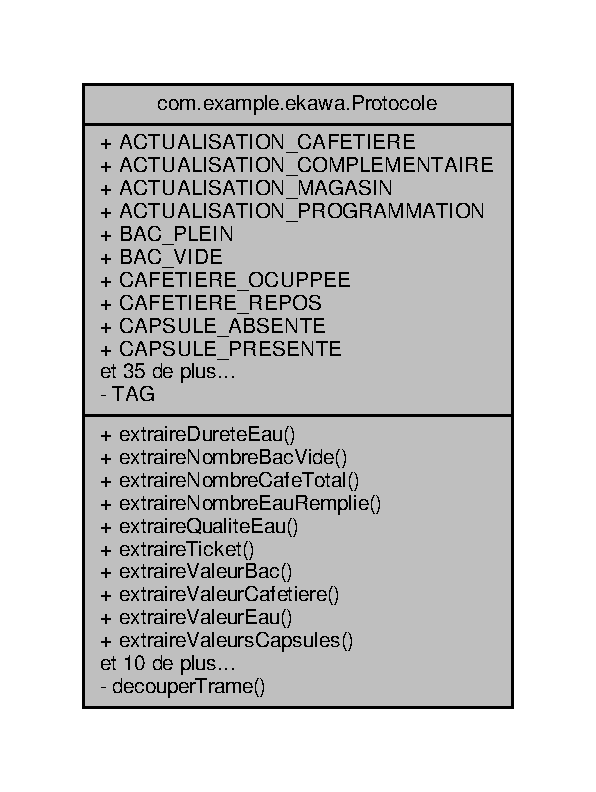
\includegraphics[width=286pt]{classcom_1_1example_1_1ekawa_1_1_protocole__coll__graph}
\end{center}
\end{figure}
\subsubsection*{Fonctions membres publiques statiques}
\begin{DoxyCompactItemize}
\item 
static int \hyperlink{classcom_1_1example_1_1ekawa_1_1_protocole_a3d092fccea3a5bf3a92810dbe90603b0}{extraire\+Durete\+Eau} (String trame)
\begin{DoxyCompactList}\small\item\em Methode qui permet d\textquotesingle{}extraire la dureté de l\textquotesingle{}eau. \end{DoxyCompactList}\item 
static int \hyperlink{classcom_1_1example_1_1ekawa_1_1_protocole_a7cdbcbd7aa67f4b0cebb963725b0c67e}{extraire\+Nombre\+Bac\+Vide} (String trame)
\begin{DoxyCompactList}\small\item\em Methode qui permet d\textquotesingle{}extraire le nombre de bac vidé \end{DoxyCompactList}\item 
static int \hyperlink{classcom_1_1example_1_1ekawa_1_1_protocole_ad76b79c64aaa9abed9a1219f3f28cb9a}{extraire\+Nombre\+Cafe\+Total} (String trame)
\begin{DoxyCompactList}\small\item\em Methode qui permet d\textquotesingle{}extraire le nombre de cafe effectué au total. \end{DoxyCompactList}\item 
static int \hyperlink{classcom_1_1example_1_1ekawa_1_1_protocole_ae4aa9859ca0f359284c931e31732477f}{extraire\+Nombre\+Eau\+Remplie} (String trame)
\begin{DoxyCompactList}\small\item\em Methode qui permet d\textquotesingle{}extraire le nombre d\textquotesingle{}eau remplie. \end{DoxyCompactList}\item 
static int \hyperlink{classcom_1_1example_1_1ekawa_1_1_protocole_a8f7c96aaa3fad76354e1cb4665c85e57}{extraire\+Qualite\+Eau} (String trame)
\begin{DoxyCompactList}\small\item\em Methode qui permet d\textquotesingle{}extraire la qualité de l\textquotesingle{}eau. \end{DoxyCompactList}\item 
static int \hyperlink{classcom_1_1example_1_1ekawa_1_1_protocole_a4997ef198a7f87d76c2f68849caae8d7}{extraire\+Ticket} (String trame)
\item 
static boolean \hyperlink{classcom_1_1example_1_1ekawa_1_1_protocole_a235ca0a3c40a50f4dc75346a60e54917}{extraire\+Valeur\+Bac} (String trame)
\begin{DoxyCompactList}\small\item\em Methode qui permet d\textquotesingle{}extraire la valeur du bac. \end{DoxyCompactList}\item 
static boolean \hyperlink{classcom_1_1example_1_1ekawa_1_1_protocole_abc2f21c6245695c5037bd0a2eac88799}{extraire\+Valeur\+Cafetiere} (String trame)
\begin{DoxyCompactList}\small\item\em Methode qui permet d\textquotesingle{}extraire la valeur de la cafetère. \end{DoxyCompactList}\item 
static int \hyperlink{classcom_1_1example_1_1ekawa_1_1_protocole_ad979442926a41d39052501267b5f5be3}{extraire\+Valeur\+Eau} (String trame)
\begin{DoxyCompactList}\small\item\em Methode qui permet d\textquotesingle{}extraire le niveau d\textquotesingle{}eau. \end{DoxyCompactList}\item 
static boolean \mbox{[}$\,$\mbox{]} \hyperlink{classcom_1_1example_1_1ekawa_1_1_protocole_ab9ea349bfe2b76585f8e71677cacd867}{extraire\+Valeurs\+Capsules} (String trame)
\begin{DoxyCompactList}\small\item\em Methode qui permet les etats des capsules. \end{DoxyCompactList}\item 
static boolean \hyperlink{classcom_1_1example_1_1ekawa_1_1_protocole_ae5e80461f082b4d2e469ee6841b9a380}{extraire\+Valeur\+Tasse} (String trame)
\begin{DoxyCompactList}\small\item\em Methode qui permet d\textquotesingle{}extraire la valeur de la tasse. \end{DoxyCompactList}\item 
static boolean \hyperlink{classcom_1_1example_1_1ekawa_1_1_protocole_add9d5727209d29af21fa468e6929fe0b}{extraire\+Verification} (String trame)
\begin{DoxyCompactList}\small\item\em Methode qui permet d\textquotesingle{}extraire la vérification. \end{DoxyCompactList}\item 
static String \hyperlink{classcom_1_1example_1_1ekawa_1_1_protocole_a71e172b9adefa345ebff98663129f833}{fabriquer\+Trame\+Actualisation\+Cafetiere} ()
\begin{DoxyCompactList}\small\item\em Methode qui permet de créer une trame pour actualiser les données de la cafetière. \end{DoxyCompactList}\item 
static String \hyperlink{classcom_1_1example_1_1ekawa_1_1_protocole_a4a7fde713ecc0e7d8653f4610b58f1bf}{fabriquer\+Trame\+Actualisation\+Complementaires} ()
\begin{DoxyCompactList}\small\item\em Methode qui permet de créer une trame pour actualiser les données complémentaires. \end{DoxyCompactList}\item 
static String \hyperlink{classcom_1_1example_1_1ekawa_1_1_protocole_aec8d32eecd3d497bc6c3d94c6e29450c}{fabriquer\+Trame\+Actualisation\+Magasin} ()
\begin{DoxyCompactList}\small\item\em Methode qui permet de créer une trame pour actualiser les données du magasin. \end{DoxyCompactList}\item 
static String \hyperlink{classcom_1_1example_1_1ekawa_1_1_protocole_ac967186423a451ede7e4b9bc16a96222}{fabriquer\+Trame\+Creer\+Programmation} (int capsule, int boisson, int jour, String heure, int frequence)
\begin{DoxyCompactList}\small\item\em Methode qui permet de créer une trame pour créer une programmation. \end{DoxyCompactList}\item 
static String \hyperlink{classcom_1_1example_1_1ekawa_1_1_protocole_a95497419a17cd6ba14663af6c20d7797}{fabriquer\+Trame\+Preparation\+Cafe} (int boisson\+Actuelle, int capsule\+Actuelle)
\begin{DoxyCompactList}\small\item\em Methode qui permet de créer une trame pour lancer la préparation d\textquotesingle{}un café \end{DoxyCompactList}\item 
static String \hyperlink{classcom_1_1example_1_1ekawa_1_1_protocole_a7b6e2d90184a17cdf7ee63b350486b3a}{fabriquer\+Trame\+Reinitialiser} ()
\begin{DoxyCompactList}\small\item\em Methode qui permet de créer une trame pour réinitialiser les données complémentaires. \end{DoxyCompactList}\item 
static String \hyperlink{classcom_1_1example_1_1ekawa_1_1_protocole_afa3ca73b737062d6048c1a6cc9c8c79d}{fabriquer\+Trame\+Supprimer\+Programmation} (int ticket)
\begin{DoxyCompactList}\small\item\em Methode qui permet de créer une trame pour supprimer une programmation. \end{DoxyCompactList}\item 
static String \hyperlink{classcom_1_1example_1_1ekawa_1_1_protocole_a6a93842b8987e56582d83c778305840a}{fabriquer\+Trame\+Test\+Alive} ()
\begin{DoxyCompactList}\small\item\em Methode qui permet de créer une trame pour tester la connection avec la machine. \end{DoxyCompactList}\end{DoxyCompactItemize}
\subsubsection*{Attributs publics statiques}
\begin{DoxyCompactItemize}
\item 
static final String \hyperlink{classcom_1_1example_1_1ekawa_1_1_protocole_ab35c00ac601a9f2037ba8c95d9c09983}{A\+C\+T\+U\+A\+L\+I\+S\+A\+T\+I\+O\+N\+\_\+\+C\+A\+F\+E\+T\+I\+E\+RE} = \char`\"{}S1\char`\"{}
\item 
static final String \hyperlink{classcom_1_1example_1_1ekawa_1_1_protocole_a7751357fc287fe44de89ebd3fc9cee9b}{A\+C\+T\+U\+A\+L\+I\+S\+A\+T\+I\+O\+N\+\_\+\+C\+O\+M\+P\+L\+E\+M\+E\+N\+T\+A\+I\+RE} = \char`\"{}S3\char`\"{}
\item 
static final String \hyperlink{classcom_1_1example_1_1ekawa_1_1_protocole_a8a6313d18d5ca2b55181302f6ec96330}{A\+C\+T\+U\+A\+L\+I\+S\+A\+T\+I\+O\+N\+\_\+\+M\+A\+G\+A\+S\+IN} = \char`\"{}S2\char`\"{}
\item 
static final String \hyperlink{classcom_1_1example_1_1ekawa_1_1_protocole_a8127ee50bdfb556779ad1c920c498e83}{A\+C\+T\+U\+A\+L\+I\+S\+A\+T\+I\+O\+N\+\_\+\+P\+R\+O\+G\+R\+A\+M\+M\+A\+T\+I\+ON} = \char`\"{}S4\char`\"{}
\item 
static final String \hyperlink{classcom_1_1example_1_1ekawa_1_1_protocole_a499d999d5a6644a3f02bc63bd764e469}{B\+A\+C\+\_\+\+P\+L\+E\+IN} = \char`\"{}0\char`\"{}
\item 
static final String \hyperlink{classcom_1_1example_1_1ekawa_1_1_protocole_a790736e534bd8f87d62c5e1bdb759f45}{B\+A\+C\+\_\+\+V\+I\+DE} = \char`\"{}1\char`\"{}
\item 
static final String \hyperlink{classcom_1_1example_1_1ekawa_1_1_protocole_a6ba36890a3e7ff61391884071fc25a21}{C\+A\+F\+E\+T\+I\+E\+R\+E\+\_\+\+O\+C\+U\+P\+P\+EE} = \char`\"{}0\char`\"{}
\item 
static final String \hyperlink{classcom_1_1example_1_1ekawa_1_1_protocole_a8a1722dd819850baa7e6ca765e66c581}{C\+A\+F\+E\+T\+I\+E\+R\+E\+\_\+\+R\+E\+P\+OS} = \char`\"{}1\char`\"{}
\item 
static final String \hyperlink{classcom_1_1example_1_1ekawa_1_1_protocole_ac7b6a2008b1195eae4628de3326bf97f}{C\+A\+P\+S\+U\+L\+E\+\_\+\+A\+B\+S\+E\+N\+TE} = \char`\"{}0\char`\"{}
\item 
static final String \hyperlink{classcom_1_1example_1_1ekawa_1_1_protocole_a4cd76f0386b4691063c48c0e4d8d8e40}{C\+A\+P\+S\+U\+L\+E\+\_\+\+P\+R\+E\+S\+E\+N\+TE} = \char`\"{}1\char`\"{}
\item 
static final String \hyperlink{classcom_1_1example_1_1ekawa_1_1_protocole_a2ca55536aa2d416dbc4bf7856c6bae3c}{C\+R\+E\+E\+R\+\_\+\+P\+R\+O\+G\+R\+A\+M\+M\+A\+T\+I\+ON} = \char`\"{}P\char`\"{}
\item 
static final String \hyperlink{classcom_1_1example_1_1ekawa_1_1_protocole_a9a73b15a5d0408ae423cc6f4ff3e7c21}{D\+E\+B\+U\+T\+\_\+\+T\+R\+A\+ME} = \char`\"{}\$ekawa;\char`\"{}
\item 
static final int \hyperlink{classcom_1_1example_1_1ekawa_1_1_protocole_ab60999720fc62237ae5f8c1e7921aa4d}{E\+M\+P\+L\+A\+C\+E\+M\+E\+N\+T\+\_\+\+B\+AC} = 2
\item 
static final int \hyperlink{classcom_1_1example_1_1ekawa_1_1_protocole_af6d747772dbddcd7e7b76745174645f0}{E\+M\+P\+L\+A\+C\+E\+M\+E\+N\+T\+\_\+\+C\+A\+F\+E\+T\+I\+E\+RE} = 0
\item 
static final int \hyperlink{classcom_1_1example_1_1ekawa_1_1_protocole_a9345f9120d147cf525afc440f4746129}{E\+M\+P\+L\+A\+C\+E\+M\+E\+N\+T\+\_\+\+D\+U\+R\+E\+T\+E\+\_\+\+E\+AU} = 3
\item 
static final int \hyperlink{classcom_1_1example_1_1ekawa_1_1_protocole_a2a6093ce136870c13b2ace7e46be9a5f}{E\+M\+P\+L\+A\+C\+E\+M\+E\+N\+T\+\_\+\+E\+AU} = 3
\item 
static final int \hyperlink{classcom_1_1example_1_1ekawa_1_1_protocole_ac637e46d16d675adb3c0729055d259cd}{E\+M\+P\+L\+A\+C\+E\+M\+E\+N\+T\+\_\+\+N\+B\+\_\+\+B\+A\+C\+\_\+\+V\+I\+D\+EE} = 1
\item 
static final int \hyperlink{classcom_1_1example_1_1ekawa_1_1_protocole_a328dc7d5ae0030abea78746a469d0301}{E\+M\+P\+L\+A\+C\+E\+M\+E\+N\+T\+\_\+\+N\+B\+\_\+\+C\+A\+FE} = 0
\item 
static final int \hyperlink{classcom_1_1example_1_1ekawa_1_1_protocole_a3c7e43fc0589bd18f2e4631c509cbb59}{E\+M\+P\+L\+A\+C\+E\+M\+E\+N\+T\+\_\+\+N\+B\+\_\+\+E\+A\+U\+\_\+\+R\+E\+M\+P\+L\+IE} = 2
\item 
static final int \hyperlink{classcom_1_1example_1_1ekawa_1_1_protocole_aeb21f04096c5f1220c172bfdfbdd5dae}{E\+M\+P\+L\+A\+C\+E\+M\+E\+N\+T\+\_\+\+Q\+U\+A\+L\+I\+T\+E\+\_\+\+E\+AU} = 4
\item 
static final int \hyperlink{classcom_1_1example_1_1ekawa_1_1_protocole_a4e694989f44fe628753f5e65f6c8c08e}{E\+M\+P\+L\+A\+C\+E\+M\+E\+N\+T\+\_\+\+R\+E\+T\+O\+UR} = 0
\item 
static final int \hyperlink{classcom_1_1example_1_1ekawa_1_1_protocole_a2ca3da411b9d68caf3ac2ff0cdf55216}{E\+M\+P\+L\+A\+C\+E\+M\+E\+N\+T\+\_\+\+T\+A\+S\+SE} = 1
\item 
static final int \hyperlink{classcom_1_1example_1_1ekawa_1_1_protocole_a6250b8095974b868336c880dc5c68f7f}{E\+M\+P\+L\+A\+C\+E\+M\+E\+N\+T\+\_\+\+T\+I\+C\+K\+ET} = 0
\item 
static final int \hyperlink{classcom_1_1example_1_1ekawa_1_1_protocole_ae76a20c0852f58c7dd77110816d8d809}{E\+M\+P\+L\+A\+C\+E\+M\+E\+N\+T\+\_\+\+V\+E\+R\+I\+F\+I\+C\+A\+T\+I\+ON} = 0
\item 
static final int \hyperlink{classcom_1_1example_1_1ekawa_1_1_protocole_aab437189a20d6f6447262ed50c666bde}{E\+M\+P\+L\+A\+C\+E\+M\+E\+N\+T\+\_\+\+V\+E\+R\+I\+F\+I\+C\+A\+T\+I\+O\+N\+\_\+\+P\+R\+O\+G\+R\+A\+M\+M\+A\+T\+I\+ON} = 1
\item 
static final int \hyperlink{classcom_1_1example_1_1ekawa_1_1_protocole_a18dec2fc4aa359cbcb7a7fe04ea5614a}{E\+R\+R\+E\+U\+R\+\_\+\+T\+I\+C\+K\+ET} = 0
\item 
static final String \hyperlink{classcom_1_1example_1_1ekawa_1_1_protocole_aece1e2c0e4110c3d91fb69da213e847f}{F\+I\+N\+\_\+\+T\+R\+A\+ME} = \char`\"{}\textbackslash{}r\textbackslash{}n\char`\"{}
\item 
static final String \hyperlink{classcom_1_1example_1_1ekawa_1_1_protocole_acb81150b5809d8635dd3301fa376a1d6}{I\+N\+D\+I\+C\+A\+T\+E\+U\+R\+\_\+\+P\+R\+E\+P\+A\+R\+A\+T\+I\+O\+N\+\_\+\+C\+A\+FE} = \char`\"{}C\char`\"{}
\item 
static final Integer \hyperlink{classcom_1_1example_1_1ekawa_1_1_protocole_a4318fa7c5638fd5da231029d1e2e9c99}{N\+I\+V\+E\+A\+U\+\_\+\+E\+A\+U\+\_\+\+M\+AX} = 100
\begin{DoxyCompactList}\small\item\em Le niveau d\textquotesingle{}eau max. \end{DoxyCompactList}\item 
static final Integer \hyperlink{classcom_1_1example_1_1ekawa_1_1_protocole_abba816d4dfe88be3a873669f2056aecc}{N\+I\+V\+E\+A\+U\+\_\+\+E\+A\+U\+\_\+\+M\+IN} = 0
\begin{DoxyCompactList}\small\item\em Le niveau d\textquotesingle{}eau min. \end{DoxyCompactList}\item 
static final String \hyperlink{classcom_1_1example_1_1ekawa_1_1_protocole_add67f8989ac6672f498b8c9f085cd445}{R\+E\+I\+N\+I\+T\+I\+A\+L\+I\+S\+ER} = \char`\"{}R\char`\"{}
\item 
static final int \hyperlink{classcom_1_1example_1_1ekawa_1_1_protocole_ad0aa6e75515c4a47cf40a32ef5d88928}{R\+E\+I\+N\+I\+T\+I\+A\+L\+I\+S\+E\+R\+\_\+\+D\+U\+R\+E\+T\+E\+\_\+\+E\+AU} = 0
\item 
static final int \hyperlink{classcom_1_1example_1_1ekawa_1_1_protocole_a534fcc2db3caed0e7e6f969edde12f4d}{R\+E\+I\+N\+I\+T\+I\+A\+L\+I\+S\+E\+R\+\_\+\+N\+B\+\_\+\+B\+A\+C\+\_\+\+V\+I\+D\+EE} = 1
\item 
static final int \hyperlink{classcom_1_1example_1_1ekawa_1_1_protocole_ab93072e61ae443c91f07700a3f754a1c}{R\+E\+I\+N\+I\+T\+I\+A\+L\+I\+S\+E\+R\+\_\+\+N\+B\+\_\+\+C\+A\+FE} = 1
\item 
static final int \hyperlink{classcom_1_1example_1_1ekawa_1_1_protocole_a627d052e923e3445296c0ea539ebc018}{R\+E\+I\+N\+I\+T\+I\+A\+L\+I\+S\+E\+R\+\_\+\+N\+B\+\_\+\+E\+A\+U\+\_\+\+R\+E\+M\+P\+L\+IE} = 1
\item 
static final int \hyperlink{classcom_1_1example_1_1ekawa_1_1_protocole_a2586e1d3430677cd425f4a462819c10c}{R\+E\+I\+N\+I\+T\+I\+A\+L\+I\+S\+E\+R\+\_\+\+P\+R\+O\+G\+R\+A\+M\+M\+A\+T\+I\+O\+NS} = 1
\item 
static final int \hyperlink{classcom_1_1example_1_1ekawa_1_1_protocole_a201cf97045945715a64c2b055e9a59c3}{R\+E\+I\+N\+I\+T\+I\+A\+L\+I\+S\+E\+R\+\_\+\+Q\+U\+A\+L\+I\+T\+E\+\_\+\+E\+AU} = 0
\item 
static final char \hyperlink{classcom_1_1example_1_1ekawa_1_1_protocole_ae7fcfc428ba9d1815daf59fcab12da13}{R\+E\+T\+O\+U\+R\+\_\+\+I\+N\+V\+A\+L\+I\+DE} = \textquotesingle{}0\textquotesingle{}
\item 
static final char \hyperlink{classcom_1_1example_1_1ekawa_1_1_protocole_aa9b59014b7359878297b002afa160a46}{R\+E\+T\+O\+U\+R\+\_\+\+V\+A\+L\+I\+DE} = \textquotesingle{}1\textquotesingle{}
\item 
static final String \hyperlink{classcom_1_1example_1_1ekawa_1_1_protocole_ad05ba92eb443c22bdcd6d7a5a6928558}{S\+U\+P\+P\+R\+I\+M\+E\+R\+\_\+\+P\+R\+O\+G\+R\+A\+M\+M\+A\+T\+I\+ON} = \char`\"{}S\char`\"{}
\item 
static final String \hyperlink{classcom_1_1example_1_1ekawa_1_1_protocole_aec2265bfb60660cbf5dfb716f694bcfb}{T\+A\+S\+S\+E\+\_\+\+A\+B\+S\+E\+N\+TE} = \char`\"{}0\char`\"{}
\item 
static final String \hyperlink{classcom_1_1example_1_1ekawa_1_1_protocole_a2f969365d74ec301bc9d76fb992ed9e6}{T\+A\+S\+S\+E\+\_\+\+P\+R\+E\+S\+E\+N\+TE} = \char`\"{}1\char`\"{}
\item 
static final String \hyperlink{classcom_1_1example_1_1ekawa_1_1_protocole_a710b865b4ce664d2adda2f5d5ccd6a72}{T\+E\+S\+T\+\_\+\+A\+L\+I\+VE} = \char`\"{}A\char`\"{}
\item 
static final int \hyperlink{classcom_1_1example_1_1ekawa_1_1_protocole_a85fcaa3a9fda1a44914a52d0c2f79ed9}{V\+E\+R\+I\+F\+I\+C\+A\+T\+I\+O\+N\+\_\+\+I\+N\+V\+A\+L\+I\+DE} = 0
\item 
static final int \hyperlink{classcom_1_1example_1_1ekawa_1_1_protocole_a9a84f1d8388a25297e50fbc3d293ecf3}{V\+E\+R\+I\+F\+I\+C\+A\+T\+I\+O\+N\+\_\+\+V\+A\+L\+I\+DE} = 1
\end{DoxyCompactItemize}
\subsubsection*{Fonctions membres privées statiques}
\begin{DoxyCompactItemize}
\item 
static String \mbox{[}$\,$\mbox{]} \hyperlink{classcom_1_1example_1_1ekawa_1_1_protocole_a23c261e4ab5ad3c2ac60187f04ae40ea}{decouper\+Trame} (String trame)
\begin{DoxyCompactList}\small\item\em Methode qui permet de découper une trame. \end{DoxyCompactList}\end{DoxyCompactItemize}
\subsubsection*{Attributs privés statiques}
\begin{DoxyCompactItemize}
\item 
static final String \hyperlink{classcom_1_1example_1_1ekawa_1_1_protocole_ae9b68fa0daac528421b887f19413f8f5}{T\+AG} = \char`\"{}Protocole\char`\"{}
\end{DoxyCompactItemize}


\subsubsection{Description détaillée}
Définit les caractéristiques du protocole E\+K\+A\+WA. 

Définition à la ligne \hyperlink{_protocole_8java_source_l00017}{17} du fichier \hyperlink{_protocole_8java_source}{Protocole.\+java}.



\subsubsection{Documentation des fonctions membres}
\mbox{\Hypertarget{classcom_1_1example_1_1ekawa_1_1_protocole_a23c261e4ab5ad3c2ac60187f04ae40ea}\label{classcom_1_1example_1_1ekawa_1_1_protocole_a23c261e4ab5ad3c2ac60187f04ae40ea}} 
\index{com\+::example\+::ekawa\+::\+Protocole@{com\+::example\+::ekawa\+::\+Protocole}!decouper\+Trame@{decouper\+Trame}}
\index{decouper\+Trame@{decouper\+Trame}!com\+::example\+::ekawa\+::\+Protocole@{com\+::example\+::ekawa\+::\+Protocole}}
\paragraph{\texorpdfstring{decouper\+Trame()}{decouperTrame()}}
{\footnotesize\ttfamily static String \mbox{[}$\,$\mbox{]} com.\+example.\+ekawa.\+Protocole.\+decouper\+Trame (\begin{DoxyParamCaption}\item[{String}]{trame }\end{DoxyParamCaption})\hspace{0.3cm}{\ttfamily [static]}, {\ttfamily [private]}}



Methode qui permet de découper une trame. 


\begin{DoxyParams}{Paramètres}
{\em trame} & la trame a découper \\
\hline
\end{DoxyParams}
\begin{DoxyReturn}{Renvoie}
String\mbox{[}\mbox{]} les données de la trame 
\end{DoxyReturn}


Définition à la ligne \hyperlink{_protocole_8java_source_l00208}{208} du fichier \hyperlink{_protocole_8java_source}{Protocole.\+java}.



Références \hyperlink{_protocole_8java_source_l00034}{com.\+example.\+ekawa.\+Protocole.\+A\+C\+T\+U\+A\+L\+I\+S\+A\+T\+I\+O\+N\+\_\+\+C\+A\+F\+E\+T\+I\+E\+RE}, \hyperlink{_protocole_8java_source_l00036}{com.\+example.\+ekawa.\+Protocole.\+A\+C\+T\+U\+A\+L\+I\+S\+A\+T\+I\+O\+N\+\_\+\+C\+O\+M\+P\+L\+E\+M\+E\+N\+T\+A\+I\+RE}, \hyperlink{_protocole_8java_source_l00035}{com.\+example.\+ekawa.\+Protocole.\+A\+C\+T\+U\+A\+L\+I\+S\+A\+T\+I\+O\+N\+\_\+\+M\+A\+G\+A\+S\+IN}, \hyperlink{_protocole_8java_source_l00037}{com.\+example.\+ekawa.\+Protocole.\+A\+C\+T\+U\+A\+L\+I\+S\+A\+T\+I\+O\+N\+\_\+\+P\+R\+O\+G\+R\+A\+M\+M\+A\+T\+I\+ON}, \hyperlink{_protocole_8java_source_l00032}{com.\+example.\+ekawa.\+Protocole.\+C\+R\+E\+E\+R\+\_\+\+P\+R\+O\+G\+R\+A\+M\+M\+A\+T\+I\+ON}, \hyperlink{_protocole_8java_source_l00031}{com.\+example.\+ekawa.\+Protocole.\+R\+E\+I\+N\+I\+T\+I\+A\+L\+I\+S\+ER}, et \hyperlink{_protocole_8java_source_l00033}{com.\+example.\+ekawa.\+Protocole.\+S\+U\+P\+P\+R\+I\+M\+E\+R\+\_\+\+P\+R\+O\+G\+R\+A\+M\+M\+A\+T\+I\+ON}.



Référencé par \hyperlink{_protocole_8java_source_l00394}{com.\+example.\+ekawa.\+Protocole.\+extraire\+Durete\+Eau()}, \hyperlink{_protocole_8java_source_l00360}{com.\+example.\+ekawa.\+Protocole.\+extraire\+Nombre\+Bac\+Vide()}, \hyperlink{_protocole_8java_source_l00343}{com.\+example.\+ekawa.\+Protocole.\+extraire\+Nombre\+Cafe\+Total()}, \hyperlink{_protocole_8java_source_l00377}{com.\+example.\+ekawa.\+Protocole.\+extraire\+Nombre\+Eau\+Remplie()}, \hyperlink{_protocole_8java_source_l00411}{com.\+example.\+ekawa.\+Protocole.\+extraire\+Qualite\+Eau()}, \hyperlink{_protocole_8java_source_l00423}{com.\+example.\+ekawa.\+Protocole.\+extraire\+Ticket()}, \hyperlink{_protocole_8java_source_l00277}{com.\+example.\+ekawa.\+Protocole.\+extraire\+Valeur\+Bac()}, \hyperlink{_protocole_8java_source_l00233}{com.\+example.\+ekawa.\+Protocole.\+extraire\+Valeur\+Cafetiere()}, \hyperlink{_protocole_8java_source_l00299}{com.\+example.\+ekawa.\+Protocole.\+extraire\+Valeur\+Eau()}, \hyperlink{_protocole_8java_source_l00319}{com.\+example.\+ekawa.\+Protocole.\+extraire\+Valeurs\+Capsules()}, \hyperlink{_protocole_8java_source_l00255}{com.\+example.\+ekawa.\+Protocole.\+extraire\+Valeur\+Tasse()}, et \hyperlink{_protocole_8java_source_l00440}{com.\+example.\+ekawa.\+Protocole.\+extraire\+Verification()}.


\begin{DoxyCode}
00209     \{
00210         Log.d(\hyperlink{classcom_1_1example_1_1ekawa_1_1_protocole_ae9b68fa0daac528421b887f19413f8f5}{TAG}, \textcolor{stringliteral}{"decouperTrame()"});
00211         \textcolor{keywordflow}{if}(trame.startsWith(Protocole.ACTUALISATION\_CAFETIERE))
00212             trame = trame.replace(Protocole.ACTUALISATION\_CAFETIERE + \textcolor{charliteral}{';'}, \textcolor{stringliteral}{""});
00213         \textcolor{keywordflow}{else} \textcolor{keywordflow}{if}(trame.startsWith(Protocole.ACTUALISATION\_MAGASIN))
00214             trame = trame.replace(Protocole.ACTUALISATION\_MAGASIN + \textcolor{charliteral}{';'}, \textcolor{stringliteral}{""});
00215         \textcolor{keywordflow}{else} \textcolor{keywordflow}{if}(trame.startsWith(Protocole.ACTUALISATION\_COMPLEMENTAIRE))
00216             trame = trame.replace(Protocole.ACTUALISATION\_COMPLEMENTAIRE + \textcolor{stringliteral}{";"}, \textcolor{stringliteral}{""});
00217         \textcolor{keywordflow}{else} \textcolor{keywordflow}{if}(trame.startsWith(Protocole.ACTUALISATION\_PROGRAMMATION))
00218             trame = trame.replace(Protocole.ACTUALISATION\_PROGRAMMATION + \textcolor{stringliteral}{";"}, \textcolor{stringliteral}{""});
00219         \textcolor{keywordflow}{else} \textcolor{keywordflow}{if}(trame.startsWith(Protocole.REINITIALISER))
00220             trame = trame.replace(Protocole.REINITIALISER + \textcolor{stringliteral}{";"}, \textcolor{stringliteral}{""});
00221         \textcolor{keywordflow}{else} \textcolor{keywordflow}{if}(trame.startsWith(Protocole.CREER\_PROGRAMMATION))
00222             trame = trame.replace(Protocole.CREER\_PROGRAMMATION + \textcolor{stringliteral}{";"}, \textcolor{stringliteral}{""});
00223         \textcolor{keywordflow}{else} \textcolor{keywordflow}{if}(trame.startsWith(Protocole.SUPPRIMER\_PROGRAMMATION))
00224             trame = trame.replace(Protocole.SUPPRIMER\_PROGRAMMATION + \textcolor{stringliteral}{";"}, \textcolor{stringliteral}{""});
00225         \textcolor{keywordflow}{return} trame.split(\textcolor{stringliteral}{";"});
00226     \}
\end{DoxyCode}
\mbox{\Hypertarget{classcom_1_1example_1_1ekawa_1_1_protocole_a3d092fccea3a5bf3a92810dbe90603b0}\label{classcom_1_1example_1_1ekawa_1_1_protocole_a3d092fccea3a5bf3a92810dbe90603b0}} 
\index{com\+::example\+::ekawa\+::\+Protocole@{com\+::example\+::ekawa\+::\+Protocole}!extraire\+Durete\+Eau@{extraire\+Durete\+Eau}}
\index{extraire\+Durete\+Eau@{extraire\+Durete\+Eau}!com\+::example\+::ekawa\+::\+Protocole@{com\+::example\+::ekawa\+::\+Protocole}}
\paragraph{\texorpdfstring{extraire\+Durete\+Eau()}{extraireDureteEau()}}
{\footnotesize\ttfamily static int com.\+example.\+ekawa.\+Protocole.\+extraire\+Durete\+Eau (\begin{DoxyParamCaption}\item[{String}]{trame }\end{DoxyParamCaption})\hspace{0.3cm}{\ttfamily [static]}}



Methode qui permet d\textquotesingle{}extraire la dureté de l\textquotesingle{}eau. 


\begin{DoxyParams}{Paramètres}
{\em trame} & la trame recue \\
\hline
\end{DoxyParams}
\begin{DoxyReturn}{Renvoie}
int la dureté de l\textquotesingle{}eau 
\end{DoxyReturn}


Définition à la ligne \hyperlink{_protocole_8java_source_l00394}{394} du fichier \hyperlink{_protocole_8java_source}{Protocole.\+java}.



Références \hyperlink{_protocole_8java_source_l00208}{com.\+example.\+ekawa.\+Protocole.\+decouper\+Trame()}, et \hyperlink{_protocole_8java_source_l00067}{com.\+example.\+ekawa.\+Protocole.\+E\+M\+P\+L\+A\+C\+E\+M\+E\+N\+T\+\_\+\+D\+U\+R\+E\+T\+E\+\_\+\+E\+AU}.



Référencé par \hyperlink{_cafetiere_8java_source_l00574}{com.\+example.\+ekawa.\+Cafetiere.\+actualiser\+Informations\+Complementaires()}.


\begin{DoxyCode}
00395     \{
00396         String[] valeurs = \hyperlink{classcom_1_1example_1_1ekawa_1_1_protocole_a23c261e4ab5ad3c2ac60187f04ae40ea}{decouperTrame}(trame);
00397 
00398         \textcolor{keywordtype}{int} dureteEau = 0;
00399         dureteEau = Integer.parseInt(valeurs[Protocole.EMPLACEMENT\_DURETE\_EAU]);
00400 
00401         Log.d(\hyperlink{classcom_1_1example_1_1ekawa_1_1_protocole_ae9b68fa0daac528421b887f19413f8f5}{TAG}, \textcolor{stringliteral}{"Extraire dureteEau = "} + dureteEau);
00402 
00403         \textcolor{keywordflow}{return} dureteEau;
00404     \}
\end{DoxyCode}
\mbox{\Hypertarget{classcom_1_1example_1_1ekawa_1_1_protocole_a7cdbcbd7aa67f4b0cebb963725b0c67e}\label{classcom_1_1example_1_1ekawa_1_1_protocole_a7cdbcbd7aa67f4b0cebb963725b0c67e}} 
\index{com\+::example\+::ekawa\+::\+Protocole@{com\+::example\+::ekawa\+::\+Protocole}!extraire\+Nombre\+Bac\+Vide@{extraire\+Nombre\+Bac\+Vide}}
\index{extraire\+Nombre\+Bac\+Vide@{extraire\+Nombre\+Bac\+Vide}!com\+::example\+::ekawa\+::\+Protocole@{com\+::example\+::ekawa\+::\+Protocole}}
\paragraph{\texorpdfstring{extraire\+Nombre\+Bac\+Vide()}{extraireNombreBacVide()}}
{\footnotesize\ttfamily static int com.\+example.\+ekawa.\+Protocole.\+extraire\+Nombre\+Bac\+Vide (\begin{DoxyParamCaption}\item[{String}]{trame }\end{DoxyParamCaption})\hspace{0.3cm}{\ttfamily [static]}}



Methode qui permet d\textquotesingle{}extraire le nombre de bac vidé 


\begin{DoxyParams}{Paramètres}
{\em trame} & la trame recue \\
\hline
\end{DoxyParams}
\begin{DoxyReturn}{Renvoie}
int le nombre de bac vidé 
\end{DoxyReturn}


Définition à la ligne \hyperlink{_protocole_8java_source_l00360}{360} du fichier \hyperlink{_protocole_8java_source}{Protocole.\+java}.



Références \hyperlink{_protocole_8java_source_l00208}{com.\+example.\+ekawa.\+Protocole.\+decouper\+Trame()}, et \hyperlink{_protocole_8java_source_l00065}{com.\+example.\+ekawa.\+Protocole.\+E\+M\+P\+L\+A\+C\+E\+M\+E\+N\+T\+\_\+\+N\+B\+\_\+\+B\+A\+C\+\_\+\+V\+I\+D\+EE}.



Référencé par \hyperlink{_cafetiere_8java_source_l00574}{com.\+example.\+ekawa.\+Cafetiere.\+actualiser\+Informations\+Complementaires()}.


\begin{DoxyCode}
00361     \{
00362         String[] valeurs = \hyperlink{classcom_1_1example_1_1ekawa_1_1_protocole_a23c261e4ab5ad3c2ac60187f04ae40ea}{decouperTrame}(trame);
00363 
00364         \textcolor{keywordtype}{int} nombreBacVide = 0;
00365         nombreBacVide = Integer.parseInt(valeurs[Protocole.EMPLACEMENT\_NB\_BAC\_VIDEE]);
00366 
00367         Log.d(\hyperlink{classcom_1_1example_1_1ekawa_1_1_protocole_ae9b68fa0daac528421b887f19413f8f5}{TAG}, \textcolor{stringliteral}{"Extraire nombreBacVide = "} + nombreBacVide);
00368 
00369         \textcolor{keywordflow}{return} nombreBacVide;
00370     \}
\end{DoxyCode}
\mbox{\Hypertarget{classcom_1_1example_1_1ekawa_1_1_protocole_ad76b79c64aaa9abed9a1219f3f28cb9a}\label{classcom_1_1example_1_1ekawa_1_1_protocole_ad76b79c64aaa9abed9a1219f3f28cb9a}} 
\index{com\+::example\+::ekawa\+::\+Protocole@{com\+::example\+::ekawa\+::\+Protocole}!extraire\+Nombre\+Cafe\+Total@{extraire\+Nombre\+Cafe\+Total}}
\index{extraire\+Nombre\+Cafe\+Total@{extraire\+Nombre\+Cafe\+Total}!com\+::example\+::ekawa\+::\+Protocole@{com\+::example\+::ekawa\+::\+Protocole}}
\paragraph{\texorpdfstring{extraire\+Nombre\+Cafe\+Total()}{extraireNombreCafeTotal()}}
{\footnotesize\ttfamily static int com.\+example.\+ekawa.\+Protocole.\+extraire\+Nombre\+Cafe\+Total (\begin{DoxyParamCaption}\item[{String}]{trame }\end{DoxyParamCaption})\hspace{0.3cm}{\ttfamily [static]}}



Methode qui permet d\textquotesingle{}extraire le nombre de cafe effectué au total. 


\begin{DoxyParams}{Paramètres}
{\em trame} & la trame recue \\
\hline
\end{DoxyParams}
\begin{DoxyReturn}{Renvoie}
int le nombre de cafe effectué au total 
\end{DoxyReturn}


Définition à la ligne \hyperlink{_protocole_8java_source_l00343}{343} du fichier \hyperlink{_protocole_8java_source}{Protocole.\+java}.



Références \hyperlink{_protocole_8java_source_l00208}{com.\+example.\+ekawa.\+Protocole.\+decouper\+Trame()}, et \hyperlink{_protocole_8java_source_l00064}{com.\+example.\+ekawa.\+Protocole.\+E\+M\+P\+L\+A\+C\+E\+M\+E\+N\+T\+\_\+\+N\+B\+\_\+\+C\+A\+FE}.



Référencé par \hyperlink{_cafetiere_8java_source_l00574}{com.\+example.\+ekawa.\+Cafetiere.\+actualiser\+Informations\+Complementaires()}.


\begin{DoxyCode}
00344     \{
00345         String[] valeurs = \hyperlink{classcom_1_1example_1_1ekawa_1_1_protocole_a23c261e4ab5ad3c2ac60187f04ae40ea}{decouperTrame}(trame);
00346 
00347         \textcolor{keywordtype}{int} nombreCafeTotal = 0;
00348         nombreCafeTotal = Integer.parseInt(valeurs[Protocole.EMPLACEMENT\_NB\_CAFE]);
00349 
00350         Log.d(\hyperlink{classcom_1_1example_1_1ekawa_1_1_protocole_ae9b68fa0daac528421b887f19413f8f5}{TAG}, \textcolor{stringliteral}{"Extraire nombreCafeTotal = "} + nombreCafeTotal);
00351 
00352         \textcolor{keywordflow}{return} nombreCafeTotal;
00353     \}
\end{DoxyCode}
\mbox{\Hypertarget{classcom_1_1example_1_1ekawa_1_1_protocole_ae4aa9859ca0f359284c931e31732477f}\label{classcom_1_1example_1_1ekawa_1_1_protocole_ae4aa9859ca0f359284c931e31732477f}} 
\index{com\+::example\+::ekawa\+::\+Protocole@{com\+::example\+::ekawa\+::\+Protocole}!extraire\+Nombre\+Eau\+Remplie@{extraire\+Nombre\+Eau\+Remplie}}
\index{extraire\+Nombre\+Eau\+Remplie@{extraire\+Nombre\+Eau\+Remplie}!com\+::example\+::ekawa\+::\+Protocole@{com\+::example\+::ekawa\+::\+Protocole}}
\paragraph{\texorpdfstring{extraire\+Nombre\+Eau\+Remplie()}{extraireNombreEauRemplie()}}
{\footnotesize\ttfamily static int com.\+example.\+ekawa.\+Protocole.\+extraire\+Nombre\+Eau\+Remplie (\begin{DoxyParamCaption}\item[{String}]{trame }\end{DoxyParamCaption})\hspace{0.3cm}{\ttfamily [static]}}



Methode qui permet d\textquotesingle{}extraire le nombre d\textquotesingle{}eau remplie. 


\begin{DoxyParams}{Paramètres}
{\em trame} & la trame recue \\
\hline
\end{DoxyParams}
\begin{DoxyReturn}{Renvoie}
int le nombre d\textquotesingle{}eau remplie 
\end{DoxyReturn}


Définition à la ligne \hyperlink{_protocole_8java_source_l00377}{377} du fichier \hyperlink{_protocole_8java_source}{Protocole.\+java}.



Références \hyperlink{_protocole_8java_source_l00208}{com.\+example.\+ekawa.\+Protocole.\+decouper\+Trame()}, et \hyperlink{_protocole_8java_source_l00066}{com.\+example.\+ekawa.\+Protocole.\+E\+M\+P\+L\+A\+C\+E\+M\+E\+N\+T\+\_\+\+N\+B\+\_\+\+E\+A\+U\+\_\+\+R\+E\+M\+P\+L\+IE}.



Référencé par \hyperlink{_cafetiere_8java_source_l00574}{com.\+example.\+ekawa.\+Cafetiere.\+actualiser\+Informations\+Complementaires()}.


\begin{DoxyCode}
00378     \{
00379         String[] valeurs = \hyperlink{classcom_1_1example_1_1ekawa_1_1_protocole_a23c261e4ab5ad3c2ac60187f04ae40ea}{decouperTrame}(trame);
00380 
00381         \textcolor{keywordtype}{int} nombreEauRemplie = 0;
00382         nombreEauRemplie = Integer.parseInt(valeurs[Protocole.EMPLACEMENT\_NB\_EAU\_REMPLIE]);
00383 
00384         Log.d(\hyperlink{classcom_1_1example_1_1ekawa_1_1_protocole_ae9b68fa0daac528421b887f19413f8f5}{TAG}, \textcolor{stringliteral}{"Extraire nombreEauRemplie = "} + nombreEauRemplie);
00385 
00386         \textcolor{keywordflow}{return} nombreEauRemplie;
00387     \}
\end{DoxyCode}
\mbox{\Hypertarget{classcom_1_1example_1_1ekawa_1_1_protocole_a8f7c96aaa3fad76354e1cb4665c85e57}\label{classcom_1_1example_1_1ekawa_1_1_protocole_a8f7c96aaa3fad76354e1cb4665c85e57}} 
\index{com\+::example\+::ekawa\+::\+Protocole@{com\+::example\+::ekawa\+::\+Protocole}!extraire\+Qualite\+Eau@{extraire\+Qualite\+Eau}}
\index{extraire\+Qualite\+Eau@{extraire\+Qualite\+Eau}!com\+::example\+::ekawa\+::\+Protocole@{com\+::example\+::ekawa\+::\+Protocole}}
\paragraph{\texorpdfstring{extraire\+Qualite\+Eau()}{extraireQualiteEau()}}
{\footnotesize\ttfamily static int com.\+example.\+ekawa.\+Protocole.\+extraire\+Qualite\+Eau (\begin{DoxyParamCaption}\item[{String}]{trame }\end{DoxyParamCaption})\hspace{0.3cm}{\ttfamily [static]}}



Methode qui permet d\textquotesingle{}extraire la qualité de l\textquotesingle{}eau. 


\begin{DoxyParams}{Paramètres}
{\em trame} & la trame recue \\
\hline
\end{DoxyParams}
\begin{DoxyReturn}{Renvoie}
int la qualité de l\textquotesingle{}eau 
\end{DoxyReturn}


Définition à la ligne \hyperlink{_protocole_8java_source_l00411}{411} du fichier \hyperlink{_protocole_8java_source}{Protocole.\+java}.



Références \hyperlink{_protocole_8java_source_l00208}{com.\+example.\+ekawa.\+Protocole.\+decouper\+Trame()}, et \hyperlink{_protocole_8java_source_l00068}{com.\+example.\+ekawa.\+Protocole.\+E\+M\+P\+L\+A\+C\+E\+M\+E\+N\+T\+\_\+\+Q\+U\+A\+L\+I\+T\+E\+\_\+\+E\+AU}.



Référencé par \hyperlink{_cafetiere_8java_source_l00574}{com.\+example.\+ekawa.\+Cafetiere.\+actualiser\+Informations\+Complementaires()}.


\begin{DoxyCode}
00412     \{
00413         String[] valeurs = \hyperlink{classcom_1_1example_1_1ekawa_1_1_protocole_a23c261e4ab5ad3c2ac60187f04ae40ea}{decouperTrame}(trame);
00414 
00415         \textcolor{keywordtype}{int} qualiteEau = 0;
00416         qualiteEau = Integer.parseInt(valeurs[Protocole.EMPLACEMENT\_QUALITE\_EAU]);
00417 
00418         Log.d(\hyperlink{classcom_1_1example_1_1ekawa_1_1_protocole_ae9b68fa0daac528421b887f19413f8f5}{TAG}, \textcolor{stringliteral}{"Extraire qualiteEau = "} + qualiteEau);
00419 
00420         \textcolor{keywordflow}{return} qualiteEau;
00421     \}
\end{DoxyCode}
\mbox{\Hypertarget{classcom_1_1example_1_1ekawa_1_1_protocole_a4997ef198a7f87d76c2f68849caae8d7}\label{classcom_1_1example_1_1ekawa_1_1_protocole_a4997ef198a7f87d76c2f68849caae8d7}} 
\index{com\+::example\+::ekawa\+::\+Protocole@{com\+::example\+::ekawa\+::\+Protocole}!extraire\+Ticket@{extraire\+Ticket}}
\index{extraire\+Ticket@{extraire\+Ticket}!com\+::example\+::ekawa\+::\+Protocole@{com\+::example\+::ekawa\+::\+Protocole}}
\paragraph{\texorpdfstring{extraire\+Ticket()}{extraireTicket()}}
{\footnotesize\ttfamily static int com.\+example.\+ekawa.\+Protocole.\+extraire\+Ticket (\begin{DoxyParamCaption}\item[{String}]{trame }\end{DoxyParamCaption})\hspace{0.3cm}{\ttfamily [static]}}



Définition à la ligne \hyperlink{_protocole_8java_source_l00423}{423} du fichier \hyperlink{_protocole_8java_source}{Protocole.\+java}.



Références \hyperlink{_protocole_8java_source_l00208}{com.\+example.\+ekawa.\+Protocole.\+decouper\+Trame()}, et \hyperlink{_protocole_8java_source_l00090}{com.\+example.\+ekawa.\+Protocole.\+E\+M\+P\+L\+A\+C\+E\+M\+E\+N\+T\+\_\+\+T\+I\+C\+K\+ET}.



Référencé par \hyperlink{_cafetiere_8java_source_l00731}{com.\+example.\+ekawa.\+Cafetiere.\+creer\+Une\+Programmation()}, et \hyperlink{_cafetiere_8java_source_l00606}{com.\+example.\+ekawa.\+Cafetiere.\+verifier\+Programmation()}.


\begin{DoxyCode}
00424     \{
00425         String[] valeurs = \hyperlink{classcom_1_1example_1_1ekawa_1_1_protocole_a23c261e4ab5ad3c2ac60187f04ae40ea}{decouperTrame}(trame);
00426 
00427         \textcolor{keywordtype}{int} ticket = 0;
00428         ticket = Integer.parseInt(valeurs[Protocole.EMPLACEMENT\_TICKET]);
00429 
00430         Log.d(\hyperlink{classcom_1_1example_1_1ekawa_1_1_protocole_ae9b68fa0daac528421b887f19413f8f5}{TAG}, \textcolor{stringliteral}{"Extraire ticket = "} + ticket);
00431 
00432         \textcolor{keywordflow}{return} ticket;
00433     \}
\end{DoxyCode}
\mbox{\Hypertarget{classcom_1_1example_1_1ekawa_1_1_protocole_a235ca0a3c40a50f4dc75346a60e54917}\label{classcom_1_1example_1_1ekawa_1_1_protocole_a235ca0a3c40a50f4dc75346a60e54917}} 
\index{com\+::example\+::ekawa\+::\+Protocole@{com\+::example\+::ekawa\+::\+Protocole}!extraire\+Valeur\+Bac@{extraire\+Valeur\+Bac}}
\index{extraire\+Valeur\+Bac@{extraire\+Valeur\+Bac}!com\+::example\+::ekawa\+::\+Protocole@{com\+::example\+::ekawa\+::\+Protocole}}
\paragraph{\texorpdfstring{extraire\+Valeur\+Bac()}{extraireValeurBac()}}
{\footnotesize\ttfamily static boolean com.\+example.\+ekawa.\+Protocole.\+extraire\+Valeur\+Bac (\begin{DoxyParamCaption}\item[{String}]{trame }\end{DoxyParamCaption})\hspace{0.3cm}{\ttfamily [static]}}



Methode qui permet d\textquotesingle{}extraire la valeur du bac. 


\begin{DoxyParams}{Paramètres}
{\em trame} & la trame recue \\
\hline
\end{DoxyParams}
\begin{DoxyReturn}{Renvoie}
boolean la valeur du bac 
\end{DoxyReturn}


Définition à la ligne \hyperlink{_protocole_8java_source_l00277}{277} du fichier \hyperlink{_protocole_8java_source}{Protocole.\+java}.



Références \hyperlink{_protocole_8java_source_l00051}{com.\+example.\+ekawa.\+Protocole.\+B\+A\+C\+\_\+\+P\+L\+E\+IN}, \hyperlink{_protocole_8java_source_l00052}{com.\+example.\+ekawa.\+Protocole.\+B\+A\+C\+\_\+\+V\+I\+DE}, \hyperlink{_protocole_8java_source_l00208}{com.\+example.\+ekawa.\+Protocole.\+decouper\+Trame()}, et \hyperlink{_protocole_8java_source_l00050}{com.\+example.\+ekawa.\+Protocole.\+E\+M\+P\+L\+A\+C\+E\+M\+E\+N\+T\+\_\+\+B\+AC}.



Référencé par \hyperlink{_cafetiere_8java_source_l00543}{com.\+example.\+ekawa.\+Cafetiere.\+actualiser\+Cafetiere()}.


\begin{DoxyCode}
00278     \{
00279         String[] valeurs = \hyperlink{classcom_1_1example_1_1ekawa_1_1_protocole_a23c261e4ab5ad3c2ac60187f04ae40ea}{decouperTrame}(trame);
00280 
00281         \textcolor{keywordtype}{boolean} etatBac = \textcolor{keyword}{false};
00282         \textcolor{keywordflow}{if}(valeurs[Protocole.EMPLACEMENT\_BAC].equals(Protocole.BAC\_VIDE))
00283             etatBac = \textcolor{keyword}{true};
00284         \textcolor{keywordflow}{else} \textcolor{keywordflow}{if}(valeurs[Protocole.EMPLACEMENT\_BAC].equals(Protocole.BAC\_PLEIN))
00285             etatBac = \textcolor{keyword}{false};
00286         \textcolor{keywordflow}{else}
00287             Log.d(\hyperlink{classcom_1_1example_1_1ekawa_1_1_protocole_ae9b68fa0daac528421b887f19413f8f5}{TAG}, \textcolor{stringliteral}{"Erreur extraire etatBac ! "} + valeurs[Protocole.EMPLACEMENT\_BAC]);
00288 
00289         Log.d(\hyperlink{classcom_1_1example_1_1ekawa_1_1_protocole_ae9b68fa0daac528421b887f19413f8f5}{TAG}, \textcolor{stringliteral}{"Extraire etatBac = "} + etatBac);
00290 
00291         \textcolor{keywordflow}{return} etatBac;
00292     \}
\end{DoxyCode}
\mbox{\Hypertarget{classcom_1_1example_1_1ekawa_1_1_protocole_abc2f21c6245695c5037bd0a2eac88799}\label{classcom_1_1example_1_1ekawa_1_1_protocole_abc2f21c6245695c5037bd0a2eac88799}} 
\index{com\+::example\+::ekawa\+::\+Protocole@{com\+::example\+::ekawa\+::\+Protocole}!extraire\+Valeur\+Cafetiere@{extraire\+Valeur\+Cafetiere}}
\index{extraire\+Valeur\+Cafetiere@{extraire\+Valeur\+Cafetiere}!com\+::example\+::ekawa\+::\+Protocole@{com\+::example\+::ekawa\+::\+Protocole}}
\paragraph{\texorpdfstring{extraire\+Valeur\+Cafetiere()}{extraireValeurCafetiere()}}
{\footnotesize\ttfamily static boolean com.\+example.\+ekawa.\+Protocole.\+extraire\+Valeur\+Cafetiere (\begin{DoxyParamCaption}\item[{String}]{trame }\end{DoxyParamCaption})\hspace{0.3cm}{\ttfamily [static]}}



Methode qui permet d\textquotesingle{}extraire la valeur de la cafetère. 


\begin{DoxyParams}{Paramètres}
{\em trame} & la trame recue \\
\hline
\end{DoxyParams}
\begin{DoxyReturn}{Renvoie}
boolean la valeur de la cafetère 
\end{DoxyReturn}


Définition à la ligne \hyperlink{_protocole_8java_source_l00233}{233} du fichier \hyperlink{_protocole_8java_source}{Protocole.\+java}.



Références \hyperlink{_protocole_8java_source_l00041}{com.\+example.\+ekawa.\+Protocole.\+C\+A\+F\+E\+T\+I\+E\+R\+E\+\_\+\+O\+C\+U\+P\+P\+EE}, \hyperlink{_protocole_8java_source_l00042}{com.\+example.\+ekawa.\+Protocole.\+C\+A\+F\+E\+T\+I\+E\+R\+E\+\_\+\+R\+E\+P\+OS}, \hyperlink{_protocole_8java_source_l00208}{com.\+example.\+ekawa.\+Protocole.\+decouper\+Trame()}, et \hyperlink{_protocole_8java_source_l00040}{com.\+example.\+ekawa.\+Protocole.\+E\+M\+P\+L\+A\+C\+E\+M\+E\+N\+T\+\_\+\+C\+A\+F\+E\+T\+I\+E\+RE}.



Référencé par \hyperlink{_cafetiere_8java_source_l00543}{com.\+example.\+ekawa.\+Cafetiere.\+actualiser\+Cafetiere()}.


\begin{DoxyCode}
00234     \{
00235         String[] valeurs = \hyperlink{classcom_1_1example_1_1ekawa_1_1_protocole_a23c261e4ab5ad3c2ac60187f04ae40ea}{decouperTrame}(trame);
00236 
00237         \textcolor{keywordtype}{boolean} etatCafetiere = \textcolor{keyword}{false};
00238         \textcolor{keywordflow}{if}(valeurs[Protocole.EMPLACEMENT\_CAFETIERE].equals(Protocole.CAFETIERE\_REPOS))
00239             etatCafetiere = \textcolor{keyword}{true};
00240         \textcolor{keywordflow}{else} \textcolor{keywordflow}{if}(valeurs[Protocole.EMPLACEMENT\_CAFETIERE].equals(Protocole.CAFETIERE\_OCUPPEE))
00241             etatCafetiere = \textcolor{keyword}{false};
00242         \textcolor{keywordflow}{else}
00243             Log.d(\hyperlink{classcom_1_1example_1_1ekawa_1_1_protocole_ae9b68fa0daac528421b887f19413f8f5}{TAG}, \textcolor{stringliteral}{"Erreur extraire etatCafetiere ! "} + valeurs[Protocole.EMPLACEMENT\_CAFETIERE]);
00244 
00245         Log.d(\hyperlink{classcom_1_1example_1_1ekawa_1_1_protocole_ae9b68fa0daac528421b887f19413f8f5}{TAG}, \textcolor{stringliteral}{"Extraire etatCafetiere = "} + etatCafetiere);
00246 
00247         \textcolor{keywordflow}{return} etatCafetiere;
00248     \}
\end{DoxyCode}
\mbox{\Hypertarget{classcom_1_1example_1_1ekawa_1_1_protocole_ad979442926a41d39052501267b5f5be3}\label{classcom_1_1example_1_1ekawa_1_1_protocole_ad979442926a41d39052501267b5f5be3}} 
\index{com\+::example\+::ekawa\+::\+Protocole@{com\+::example\+::ekawa\+::\+Protocole}!extraire\+Valeur\+Eau@{extraire\+Valeur\+Eau}}
\index{extraire\+Valeur\+Eau@{extraire\+Valeur\+Eau}!com\+::example\+::ekawa\+::\+Protocole@{com\+::example\+::ekawa\+::\+Protocole}}
\paragraph{\texorpdfstring{extraire\+Valeur\+Eau()}{extraireValeurEau()}}
{\footnotesize\ttfamily static int com.\+example.\+ekawa.\+Protocole.\+extraire\+Valeur\+Eau (\begin{DoxyParamCaption}\item[{String}]{trame }\end{DoxyParamCaption})\hspace{0.3cm}{\ttfamily [static]}}



Methode qui permet d\textquotesingle{}extraire le niveau d\textquotesingle{}eau. 


\begin{DoxyParams}{Paramètres}
{\em trame} & la trame recue \\
\hline
\end{DoxyParams}
\begin{DoxyReturn}{Renvoie}
boolean le niveau d\textquotesingle{}eau 
\end{DoxyReturn}


Définition à la ligne \hyperlink{_protocole_8java_source_l00299}{299} du fichier \hyperlink{_protocole_8java_source}{Protocole.\+java}.



Références \hyperlink{_protocole_8java_source_l00208}{com.\+example.\+ekawa.\+Protocole.\+decouper\+Trame()}, \hyperlink{_protocole_8java_source_l00055}{com.\+example.\+ekawa.\+Protocole.\+E\+M\+P\+L\+A\+C\+E\+M\+E\+N\+T\+\_\+\+E\+AU}, \hyperlink{_protocole_8java_source_l00057}{com.\+example.\+ekawa.\+Protocole.\+N\+I\+V\+E\+A\+U\+\_\+\+E\+A\+U\+\_\+\+M\+AX}, et \hyperlink{_protocole_8java_source_l00056}{com.\+example.\+ekawa.\+Protocole.\+N\+I\+V\+E\+A\+U\+\_\+\+E\+A\+U\+\_\+\+M\+IN}.



Référencé par \hyperlink{_cafetiere_8java_source_l00543}{com.\+example.\+ekawa.\+Cafetiere.\+actualiser\+Cafetiere()}.


\begin{DoxyCode}
00300     \{
00301         String[] valeurs = \hyperlink{classcom_1_1example_1_1ekawa_1_1_protocole_a23c261e4ab5ad3c2ac60187f04ae40ea}{decouperTrame}(trame);
00302 
00303         \textcolor{keywordtype}{int} niveauEau = 0;
00304         \textcolor{keywordflow}{if}(Integer.parseInt(valeurs[Protocole.EMPLACEMENT\_EAU]) >= Protocole.NIVEAU\_EAU\_MIN && Integer.
      parseInt(valeurs[3]) <= Protocole.NIVEAU\_EAU\_MAX)
00305             niveauEau = Integer.parseInt(valeurs[Protocole.EMPLACEMENT\_EAU]);
00306         \textcolor{keywordflow}{else}
00307             Log.d(\hyperlink{classcom_1_1example_1_1ekawa_1_1_protocole_ae9b68fa0daac528421b887f19413f8f5}{TAG}, \textcolor{stringliteral}{"Erreur extraire niveauEau ! "} + valeurs[Protocole.EMPLACEMENT\_EAU]);
00308 
00309         Log.d(\hyperlink{classcom_1_1example_1_1ekawa_1_1_protocole_ae9b68fa0daac528421b887f19413f8f5}{TAG}, \textcolor{stringliteral}{"Extraire niveauEau = "} + niveauEau);
00310 
00311         \textcolor{keywordflow}{return} niveauEau;
00312     \}
\end{DoxyCode}
\mbox{\Hypertarget{classcom_1_1example_1_1ekawa_1_1_protocole_ab9ea349bfe2b76585f8e71677cacd867}\label{classcom_1_1example_1_1ekawa_1_1_protocole_ab9ea349bfe2b76585f8e71677cacd867}} 
\index{com\+::example\+::ekawa\+::\+Protocole@{com\+::example\+::ekawa\+::\+Protocole}!extraire\+Valeurs\+Capsules@{extraire\+Valeurs\+Capsules}}
\index{extraire\+Valeurs\+Capsules@{extraire\+Valeurs\+Capsules}!com\+::example\+::ekawa\+::\+Protocole@{com\+::example\+::ekawa\+::\+Protocole}}
\paragraph{\texorpdfstring{extraire\+Valeurs\+Capsules()}{extraireValeursCapsules()}}
{\footnotesize\ttfamily static boolean \mbox{[}$\,$\mbox{]} com.\+example.\+ekawa.\+Protocole.\+extraire\+Valeurs\+Capsules (\begin{DoxyParamCaption}\item[{String}]{trame }\end{DoxyParamCaption})\hspace{0.3cm}{\ttfamily [static]}}



Methode qui permet les etats des capsules. 


\begin{DoxyParams}{Paramètres}
{\em trame} & la trame recue \\
\hline
\end{DoxyParams}
\begin{DoxyReturn}{Renvoie}
boolean les etats des capsules 
\end{DoxyReturn}


Définition à la ligne \hyperlink{_protocole_8java_source_l00319}{319} du fichier \hyperlink{_protocole_8java_source}{Protocole.\+java}.



Références \hyperlink{_protocole_8java_source_l00208}{com.\+example.\+ekawa.\+Protocole.\+decouper\+Trame()}, et \hyperlink{_cafetiere_8java_source_l00029}{com.\+example.\+ekawa.\+Cafetiere.\+N\+O\+M\+B\+R\+E\+\_\+\+C\+A\+P\+S\+U\+L\+E\+\_\+\+M\+AX}.



Référencé par \hyperlink{_cafetiere_8java_source_l00561}{com.\+example.\+ekawa.\+Cafetiere.\+actualiser\+Magasin()}.


\begin{DoxyCode}
00320     \{
00321         String[] valeurs = \hyperlink{classcom_1_1example_1_1ekawa_1_1_protocole_a23c261e4ab5ad3c2ac60187f04ae40ea}{decouperTrame}(trame);
00322 
00323         \textcolor{keywordtype}{boolean}[] etatsCapsules = \textcolor{keyword}{new} \textcolor{keywordtype}{boolean}[Cafetiere.NOMBRE\_CAPSULE\_MAX];
00324         \textcolor{keywordflow}{for}(\textcolor{keywordtype}{int} i = 0; i < Cafetiere.NOMBRE\_CAPSULE\_MAX; ++i)
00325         \{
00326             \textcolor{keywordflow}{if}(valeurs[i].equals(\hyperlink{classcom_1_1example_1_1ekawa_1_1_protocole_ac7b6a2008b1195eae4628de3326bf97f}{CAPSULE\_ABSENTE}))
00327                 etatsCapsules[i] = \textcolor{keyword}{false};
00328             \textcolor{keywordflow}{else} \textcolor{keywordflow}{if}(valeurs[i].equals(\hyperlink{classcom_1_1example_1_1ekawa_1_1_protocole_a4cd76f0386b4691063c48c0e4d8d8e40}{CAPSULE\_PRESENTE}))
00329                 etatsCapsules[i] = \textcolor{keyword}{true};
00330             \textcolor{keywordflow}{else}
00331                 Log.d(\hyperlink{classcom_1_1example_1_1ekawa_1_1_protocole_ae9b68fa0daac528421b887f19413f8f5}{TAG}, \textcolor{stringliteral}{"Erreur extraire état capsule n°"} + i + \textcolor{stringliteral}{" ! "} + valeurs[i]);
00332             Log.d(\hyperlink{classcom_1_1example_1_1ekawa_1_1_protocole_ae9b68fa0daac528421b887f19413f8f5}{TAG}, \textcolor{stringliteral}{"Extraire état capsule n°"} + i + \textcolor{stringliteral}{" = "} + etatsCapsules[i]);
00333         \}
00334 
00335         \textcolor{keywordflow}{return} etatsCapsules;
00336     \}
\end{DoxyCode}
\mbox{\Hypertarget{classcom_1_1example_1_1ekawa_1_1_protocole_ae5e80461f082b4d2e469ee6841b9a380}\label{classcom_1_1example_1_1ekawa_1_1_protocole_ae5e80461f082b4d2e469ee6841b9a380}} 
\index{com\+::example\+::ekawa\+::\+Protocole@{com\+::example\+::ekawa\+::\+Protocole}!extraire\+Valeur\+Tasse@{extraire\+Valeur\+Tasse}}
\index{extraire\+Valeur\+Tasse@{extraire\+Valeur\+Tasse}!com\+::example\+::ekawa\+::\+Protocole@{com\+::example\+::ekawa\+::\+Protocole}}
\paragraph{\texorpdfstring{extraire\+Valeur\+Tasse()}{extraireValeurTasse()}}
{\footnotesize\ttfamily static boolean com.\+example.\+ekawa.\+Protocole.\+extraire\+Valeur\+Tasse (\begin{DoxyParamCaption}\item[{String}]{trame }\end{DoxyParamCaption})\hspace{0.3cm}{\ttfamily [static]}}



Methode qui permet d\textquotesingle{}extraire la valeur de la tasse. 


\begin{DoxyParams}{Paramètres}
{\em trame} & la trame recue \\
\hline
\end{DoxyParams}
\begin{DoxyReturn}{Renvoie}
boolean la valeur de la tasse 
\end{DoxyReturn}


Définition à la ligne \hyperlink{_protocole_8java_source_l00255}{255} du fichier \hyperlink{_protocole_8java_source}{Protocole.\+java}.



Références \hyperlink{_protocole_8java_source_l00208}{com.\+example.\+ekawa.\+Protocole.\+decouper\+Trame()}, \hyperlink{_protocole_8java_source_l00045}{com.\+example.\+ekawa.\+Protocole.\+E\+M\+P\+L\+A\+C\+E\+M\+E\+N\+T\+\_\+\+T\+A\+S\+SE}, \hyperlink{_protocole_8java_source_l00046}{com.\+example.\+ekawa.\+Protocole.\+T\+A\+S\+S\+E\+\_\+\+A\+B\+S\+E\+N\+TE}, et \hyperlink{_protocole_8java_source_l00047}{com.\+example.\+ekawa.\+Protocole.\+T\+A\+S\+S\+E\+\_\+\+P\+R\+E\+S\+E\+N\+TE}.



Référencé par \hyperlink{_cafetiere_8java_source_l00543}{com.\+example.\+ekawa.\+Cafetiere.\+actualiser\+Cafetiere()}.


\begin{DoxyCode}
00256     \{
00257         String[] valeurs = \hyperlink{classcom_1_1example_1_1ekawa_1_1_protocole_a23c261e4ab5ad3c2ac60187f04ae40ea}{decouperTrame}(trame);
00258 
00259         \textcolor{keywordtype}{boolean} etatTasse = \textcolor{keyword}{false};
00260         \textcolor{keywordflow}{if}(valeurs[Protocole.EMPLACEMENT\_TASSE].equals(Protocole.TASSE\_PRESENTE))
00261             etatTasse = \textcolor{keyword}{true};
00262         \textcolor{keywordflow}{else} \textcolor{keywordflow}{if}(valeurs[Protocole.EMPLACEMENT\_TASSE].equals(Protocole.TASSE\_ABSENTE))
00263             etatTasse = \textcolor{keyword}{false};
00264         \textcolor{keywordflow}{else}
00265             Log.d(\hyperlink{classcom_1_1example_1_1ekawa_1_1_protocole_ae9b68fa0daac528421b887f19413f8f5}{TAG}, \textcolor{stringliteral}{"Erreur extraire etatTasse ! "} + valeurs[Protocole.EMPLACEMENT\_TASSE]);
00266 
00267         Log.d(\hyperlink{classcom_1_1example_1_1ekawa_1_1_protocole_ae9b68fa0daac528421b887f19413f8f5}{TAG}, \textcolor{stringliteral}{"Extraire etatTasse = "} + etatTasse);
00268 
00269         \textcolor{keywordflow}{return} etatTasse;
00270     \}
\end{DoxyCode}
\mbox{\Hypertarget{classcom_1_1example_1_1ekawa_1_1_protocole_add9d5727209d29af21fa468e6929fe0b}\label{classcom_1_1example_1_1ekawa_1_1_protocole_add9d5727209d29af21fa468e6929fe0b}} 
\index{com\+::example\+::ekawa\+::\+Protocole@{com\+::example\+::ekawa\+::\+Protocole}!extraire\+Verification@{extraire\+Verification}}
\index{extraire\+Verification@{extraire\+Verification}!com\+::example\+::ekawa\+::\+Protocole@{com\+::example\+::ekawa\+::\+Protocole}}
\paragraph{\texorpdfstring{extraire\+Verification()}{extraireVerification()}}
{\footnotesize\ttfamily static boolean com.\+example.\+ekawa.\+Protocole.\+extraire\+Verification (\begin{DoxyParamCaption}\item[{String}]{trame }\end{DoxyParamCaption})\hspace{0.3cm}{\ttfamily [static]}}



Methode qui permet d\textquotesingle{}extraire la vérification. 


\begin{DoxyParams}{Paramètres}
{\em trame} & la trame recue \\
\hline
\end{DoxyParams}
\begin{DoxyReturn}{Renvoie}
boolean la vérification 
\end{DoxyReturn}


Définition à la ligne \hyperlink{_protocole_8java_source_l00440}{440} du fichier \hyperlink{_protocole_8java_source}{Protocole.\+java}.



Références \hyperlink{_protocole_8java_source_l00037}{com.\+example.\+ekawa.\+Protocole.\+A\+C\+T\+U\+A\+L\+I\+S\+A\+T\+I\+O\+N\+\_\+\+P\+R\+O\+G\+R\+A\+M\+M\+A\+T\+I\+ON}, \hyperlink{_protocole_8java_source_l00208}{com.\+example.\+ekawa.\+Protocole.\+decouper\+Trame()}, \hyperlink{_protocole_8java_source_l00084}{com.\+example.\+ekawa.\+Protocole.\+E\+M\+P\+L\+A\+C\+E\+M\+E\+N\+T\+\_\+\+V\+E\+R\+I\+F\+I\+C\+A\+T\+I\+ON}, \hyperlink{_protocole_8java_source_l00085}{com.\+example.\+ekawa.\+Protocole.\+E\+M\+P\+L\+A\+C\+E\+M\+E\+N\+T\+\_\+\+V\+E\+R\+I\+F\+I\+C\+A\+T\+I\+O\+N\+\_\+\+P\+R\+O\+G\+R\+A\+M\+M\+A\+T\+I\+ON}, et \hyperlink{_protocole_8java_source_l00087}{com.\+example.\+ekawa.\+Protocole.\+V\+E\+R\+I\+F\+I\+C\+A\+T\+I\+O\+N\+\_\+\+V\+A\+L\+I\+DE}.



Référencé par \hyperlink{_cafetiere_8java_source_l00574}{com.\+example.\+ekawa.\+Cafetiere.\+actualiser\+Informations\+Complementaires()}, \hyperlink{_cafetiere_8java_source_l00606}{com.\+example.\+ekawa.\+Cafetiere.\+verifier\+Programmation()}, et \hyperlink{_cafetiere_8java_source_l00804}{com.\+example.\+ekawa.\+Cafetiere.\+verifier\+Suppression\+Dune\+Programmation()}.


\begin{DoxyCode}
00441     \{
00442         \textcolor{keywordtype}{int} position = Protocole.EMPLACEMENT\_VERIFICATION;;
00443         \textcolor{keywordflow}{if}(trame.startsWith(Protocole.ACTUALISATION\_PROGRAMMATION))
00444             position = Protocole.EMPLACEMENT\_VERIFICATION\_PROGRAMMATION;
00445 
00446         String[] valeurs = \hyperlink{classcom_1_1example_1_1ekawa_1_1_protocole_a23c261e4ab5ad3c2ac60187f04ae40ea}{decouperTrame}(trame);
00447 
00448         \textcolor{keywordtype}{int} verification = Integer.parseInt(valeurs[position]);
00449 
00450         Log.d(\hyperlink{classcom_1_1example_1_1ekawa_1_1_protocole_ae9b68fa0daac528421b887f19413f8f5}{TAG}, \textcolor{stringliteral}{"Extraire vérification = "} + verification);
00451 
00452         \textcolor{keywordflow}{if}(verification == Protocole.VERIFICATION\_VALIDE)
00453             \textcolor{keywordflow}{return} \textcolor{keyword}{true};
00454         \textcolor{keywordflow}{return} \textcolor{keyword}{false};
00455     \}
\end{DoxyCode}
\mbox{\Hypertarget{classcom_1_1example_1_1ekawa_1_1_protocole_a71e172b9adefa345ebff98663129f833}\label{classcom_1_1example_1_1ekawa_1_1_protocole_a71e172b9adefa345ebff98663129f833}} 
\index{com\+::example\+::ekawa\+::\+Protocole@{com\+::example\+::ekawa\+::\+Protocole}!fabriquer\+Trame\+Actualisation\+Cafetiere@{fabriquer\+Trame\+Actualisation\+Cafetiere}}
\index{fabriquer\+Trame\+Actualisation\+Cafetiere@{fabriquer\+Trame\+Actualisation\+Cafetiere}!com\+::example\+::ekawa\+::\+Protocole@{com\+::example\+::ekawa\+::\+Protocole}}
\paragraph{\texorpdfstring{fabriquer\+Trame\+Actualisation\+Cafetiere()}{fabriquerTrameActualisationCafetiere()}}
{\footnotesize\ttfamily static String com.\+example.\+ekawa.\+Protocole.\+fabriquer\+Trame\+Actualisation\+Cafetiere (\begin{DoxyParamCaption}{ }\end{DoxyParamCaption})\hspace{0.3cm}{\ttfamily [static]}}



Methode qui permet de créer une trame pour actualiser les données de la cafetière. 

\begin{DoxyReturn}{Renvoie}
String la trame fabriquée 
\end{DoxyReturn}


Définition à la ligne \hyperlink{_protocole_8java_source_l00145}{145} du fichier \hyperlink{_protocole_8java_source}{Protocole.\+java}.



Références \hyperlink{_protocole_8java_source_l00034}{com.\+example.\+ekawa.\+Protocole.\+A\+C\+T\+U\+A\+L\+I\+S\+A\+T\+I\+O\+N\+\_\+\+C\+A\+F\+E\+T\+I\+E\+RE}, \hyperlink{_protocole_8java_source_l00025}{com.\+example.\+ekawa.\+Protocole.\+D\+E\+B\+U\+T\+\_\+\+T\+R\+A\+ME}, et \hyperlink{_protocole_8java_source_l00026}{com.\+example.\+ekawa.\+Protocole.\+F\+I\+N\+\_\+\+T\+R\+A\+ME}.



Référencé par \hyperlink{_cafetiere_8java_source_l00495}{com.\+example.\+ekawa.\+Cafetiere.\+actualiser\+Donnees()}.


\begin{DoxyCode}
00146     \{
00147         Log.d(\hyperlink{classcom_1_1example_1_1ekawa_1_1_protocole_ae9b68fa0daac528421b887f19413f8f5}{TAG}, \textcolor{stringliteral}{"fabriquerTrameActualisationCafetiere()"});
00148         \textcolor{keywordflow}{return} Protocole.DEBUT\_TRAME + Protocole.ACTUALISATION\_CAFETIERE + Protocole.FIN\_TRAME;
00149     \}
\end{DoxyCode}
\mbox{\Hypertarget{classcom_1_1example_1_1ekawa_1_1_protocole_a4a7fde713ecc0e7d8653f4610b58f1bf}\label{classcom_1_1example_1_1ekawa_1_1_protocole_a4a7fde713ecc0e7d8653f4610b58f1bf}} 
\index{com\+::example\+::ekawa\+::\+Protocole@{com\+::example\+::ekawa\+::\+Protocole}!fabriquer\+Trame\+Actualisation\+Complementaires@{fabriquer\+Trame\+Actualisation\+Complementaires}}
\index{fabriquer\+Trame\+Actualisation\+Complementaires@{fabriquer\+Trame\+Actualisation\+Complementaires}!com\+::example\+::ekawa\+::\+Protocole@{com\+::example\+::ekawa\+::\+Protocole}}
\paragraph{\texorpdfstring{fabriquer\+Trame\+Actualisation\+Complementaires()}{fabriquerTrameActualisationComplementaires()}}
{\footnotesize\ttfamily static String com.\+example.\+ekawa.\+Protocole.\+fabriquer\+Trame\+Actualisation\+Complementaires (\begin{DoxyParamCaption}{ }\end{DoxyParamCaption})\hspace{0.3cm}{\ttfamily [static]}}



Methode qui permet de créer une trame pour actualiser les données complémentaires. 

\begin{DoxyReturn}{Renvoie}
String la trame fabriquée 
\end{DoxyReturn}


Définition à la ligne \hyperlink{_protocole_8java_source_l00165}{165} du fichier \hyperlink{_protocole_8java_source}{Protocole.\+java}.



Références \hyperlink{_protocole_8java_source_l00036}{com.\+example.\+ekawa.\+Protocole.\+A\+C\+T\+U\+A\+L\+I\+S\+A\+T\+I\+O\+N\+\_\+\+C\+O\+M\+P\+L\+E\+M\+E\+N\+T\+A\+I\+RE}, \hyperlink{_protocole_8java_source_l00025}{com.\+example.\+ekawa.\+Protocole.\+D\+E\+B\+U\+T\+\_\+\+T\+R\+A\+ME}, et \hyperlink{_protocole_8java_source_l00026}{com.\+example.\+ekawa.\+Protocole.\+F\+I\+N\+\_\+\+T\+R\+A\+ME}.



Référencé par \hyperlink{_cafetiere_8java_source_l00495}{com.\+example.\+ekawa.\+Cafetiere.\+actualiser\+Donnees()}.


\begin{DoxyCode}
00166     \{
00167         Log.d(\hyperlink{classcom_1_1example_1_1ekawa_1_1_protocole_ae9b68fa0daac528421b887f19413f8f5}{TAG}, \textcolor{stringliteral}{"fabriquerTrameActualisationComplementaires()"});
00168         \textcolor{keywordflow}{return} Protocole.DEBUT\_TRAME + Protocole.ACTUALISATION\_COMPLEMENTAIRE + Protocole.FIN\_TRAME;
00169     \}
\end{DoxyCode}
\mbox{\Hypertarget{classcom_1_1example_1_1ekawa_1_1_protocole_aec8d32eecd3d497bc6c3d94c6e29450c}\label{classcom_1_1example_1_1ekawa_1_1_protocole_aec8d32eecd3d497bc6c3d94c6e29450c}} 
\index{com\+::example\+::ekawa\+::\+Protocole@{com\+::example\+::ekawa\+::\+Protocole}!fabriquer\+Trame\+Actualisation\+Magasin@{fabriquer\+Trame\+Actualisation\+Magasin}}
\index{fabriquer\+Trame\+Actualisation\+Magasin@{fabriquer\+Trame\+Actualisation\+Magasin}!com\+::example\+::ekawa\+::\+Protocole@{com\+::example\+::ekawa\+::\+Protocole}}
\paragraph{\texorpdfstring{fabriquer\+Trame\+Actualisation\+Magasin()}{fabriquerTrameActualisationMagasin()}}
{\footnotesize\ttfamily static String com.\+example.\+ekawa.\+Protocole.\+fabriquer\+Trame\+Actualisation\+Magasin (\begin{DoxyParamCaption}{ }\end{DoxyParamCaption})\hspace{0.3cm}{\ttfamily [static]}}



Methode qui permet de créer une trame pour actualiser les données du magasin. 

\begin{DoxyReturn}{Renvoie}
String la trame fabriquée 
\end{DoxyReturn}


Définition à la ligne \hyperlink{_protocole_8java_source_l00155}{155} du fichier \hyperlink{_protocole_8java_source}{Protocole.\+java}.



Références \hyperlink{_protocole_8java_source_l00035}{com.\+example.\+ekawa.\+Protocole.\+A\+C\+T\+U\+A\+L\+I\+S\+A\+T\+I\+O\+N\+\_\+\+M\+A\+G\+A\+S\+IN}, \hyperlink{_protocole_8java_source_l00025}{com.\+example.\+ekawa.\+Protocole.\+D\+E\+B\+U\+T\+\_\+\+T\+R\+A\+ME}, et \hyperlink{_protocole_8java_source_l00026}{com.\+example.\+ekawa.\+Protocole.\+F\+I\+N\+\_\+\+T\+R\+A\+ME}.



Référencé par \hyperlink{_cafetiere_8java_source_l00495}{com.\+example.\+ekawa.\+Cafetiere.\+actualiser\+Donnees()}.


\begin{DoxyCode}
00156     \{
00157         Log.d(\hyperlink{classcom_1_1example_1_1ekawa_1_1_protocole_ae9b68fa0daac528421b887f19413f8f5}{TAG}, \textcolor{stringliteral}{"fabriquerTrameActualisationMagasin()"});
00158         \textcolor{keywordflow}{return} Protocole.DEBUT\_TRAME + Protocole.ACTUALISATION\_MAGASIN + Protocole.FIN\_TRAME;
00159     \}
\end{DoxyCode}
\mbox{\Hypertarget{classcom_1_1example_1_1ekawa_1_1_protocole_ac967186423a451ede7e4b9bc16a96222}\label{classcom_1_1example_1_1ekawa_1_1_protocole_ac967186423a451ede7e4b9bc16a96222}} 
\index{com\+::example\+::ekawa\+::\+Protocole@{com\+::example\+::ekawa\+::\+Protocole}!fabriquer\+Trame\+Creer\+Programmation@{fabriquer\+Trame\+Creer\+Programmation}}
\index{fabriquer\+Trame\+Creer\+Programmation@{fabriquer\+Trame\+Creer\+Programmation}!com\+::example\+::ekawa\+::\+Protocole@{com\+::example\+::ekawa\+::\+Protocole}}
\paragraph{\texorpdfstring{fabriquer\+Trame\+Creer\+Programmation()}{fabriquerTrameCreerProgrammation()}}
{\footnotesize\ttfamily static String com.\+example.\+ekawa.\+Protocole.\+fabriquer\+Trame\+Creer\+Programmation (\begin{DoxyParamCaption}\item[{int}]{capsule,  }\item[{int}]{boisson,  }\item[{int}]{jour,  }\item[{String}]{heure,  }\item[{int}]{frequence }\end{DoxyParamCaption})\hspace{0.3cm}{\ttfamily [static]}}



Methode qui permet de créer une trame pour créer une programmation. 

\begin{DoxyReturn}{Renvoie}
String la trame fabriquée 
\end{DoxyReturn}


Définition à la ligne \hyperlink{_protocole_8java_source_l00175}{175} du fichier \hyperlink{_protocole_8java_source}{Protocole.\+java}.



Références \hyperlink{_protocole_8java_source_l00032}{com.\+example.\+ekawa.\+Protocole.\+C\+R\+E\+E\+R\+\_\+\+P\+R\+O\+G\+R\+A\+M\+M\+A\+T\+I\+ON}, \hyperlink{_protocole_8java_source_l00025}{com.\+example.\+ekawa.\+Protocole.\+D\+E\+B\+U\+T\+\_\+\+T\+R\+A\+ME}, et \hyperlink{_protocole_8java_source_l00026}{com.\+example.\+ekawa.\+Protocole.\+F\+I\+N\+\_\+\+T\+R\+A\+ME}.



Référencé par \hyperlink{_cafetiere_8java_source_l00720}{com.\+example.\+ekawa.\+Cafetiere.\+demander\+Creation\+Une\+Programmation()}.


\begin{DoxyCode}
00176     \{
00177         Log.d(\hyperlink{classcom_1_1example_1_1ekawa_1_1_protocole_ae9b68fa0daac528421b887f19413f8f5}{TAG}, \textcolor{stringliteral}{"fabriquerTrameCreerProgrammation()"});
00178         String trame = Protocole.DEBUT\_TRAME;
00179         trame += Protocole.CREER\_PROGRAMMATION + \textcolor{stringliteral}{";"};
00180         trame += capsule + \textcolor{stringliteral}{";"};
00181         trame += boisson + \textcolor{stringliteral}{";"};
00182         trame += jour + \textcolor{stringliteral}{";"};
00183         trame += heure + \textcolor{stringliteral}{";"};
00184         trame += frequence;
00185         trame += Protocole.FIN\_TRAME;
00186         \textcolor{keywordflow}{return} trame;
00187     \}
\end{DoxyCode}
\mbox{\Hypertarget{classcom_1_1example_1_1ekawa_1_1_protocole_a95497419a17cd6ba14663af6c20d7797}\label{classcom_1_1example_1_1ekawa_1_1_protocole_a95497419a17cd6ba14663af6c20d7797}} 
\index{com\+::example\+::ekawa\+::\+Protocole@{com\+::example\+::ekawa\+::\+Protocole}!fabriquer\+Trame\+Preparation\+Cafe@{fabriquer\+Trame\+Preparation\+Cafe}}
\index{fabriquer\+Trame\+Preparation\+Cafe@{fabriquer\+Trame\+Preparation\+Cafe}!com\+::example\+::ekawa\+::\+Protocole@{com\+::example\+::ekawa\+::\+Protocole}}
\paragraph{\texorpdfstring{fabriquer\+Trame\+Preparation\+Cafe()}{fabriquerTramePreparationCafe()}}
{\footnotesize\ttfamily static String com.\+example.\+ekawa.\+Protocole.\+fabriquer\+Trame\+Preparation\+Cafe (\begin{DoxyParamCaption}\item[{int}]{boisson\+Actuelle,  }\item[{int}]{capsule\+Actuelle }\end{DoxyParamCaption})\hspace{0.3cm}{\ttfamily [static]}}



Methode qui permet de créer une trame pour lancer la préparation d\textquotesingle{}un café 


\begin{DoxyParams}{Paramètres}
{\em boisson\+Actuelle} & la boissons actuelle \\
\hline
{\em capsule\+Actuelle} & la capsule actuelle \\
\hline
\end{DoxyParams}
\begin{DoxyReturn}{Renvoie}
String la trame fabriquée 
\end{DoxyReturn}


Définition à la ligne \hyperlink{_protocole_8java_source_l00099}{99} du fichier \hyperlink{_protocole_8java_source}{Protocole.\+java}.



Références \hyperlink{_protocole_8java_source_l00025}{com.\+example.\+ekawa.\+Protocole.\+D\+E\+B\+U\+T\+\_\+\+T\+R\+A\+ME}, \hyperlink{_protocole_8java_source_l00026}{com.\+example.\+ekawa.\+Protocole.\+F\+I\+N\+\_\+\+T\+R\+A\+ME}, et \hyperlink{_protocole_8java_source_l00030}{com.\+example.\+ekawa.\+Protocole.\+I\+N\+D\+I\+C\+A\+T\+E\+U\+R\+\_\+\+P\+R\+E\+P\+A\+R\+A\+T\+I\+O\+N\+\_\+\+C\+A\+FE}.



Référencé par \hyperlink{_cafetiere_8java_source_l00397}{com.\+example.\+ekawa.\+Cafetiere.\+demander\+Preparation\+Cafe()}.


\begin{DoxyCode}
00100     \{
00101         String trame = Protocole.DEBUT\_TRAME;
00102         trame += Protocole.INDICATEUR\_PREPARATION\_CAFE + \textcolor{stringliteral}{";"};
00103         trame += boissonActuelle + \textcolor{stringliteral}{";"};
00104         trame += capsuleActuelle;
00105         trame += Protocole.FIN\_TRAME;
00106 
00107         Log.d(\hyperlink{classcom_1_1example_1_1ekawa_1_1_protocole_ae9b68fa0daac528421b887f19413f8f5}{TAG}, \textcolor{stringliteral}{"Fabriquer trame = "} + trame);
00108 
00109         \textcolor{keywordflow}{return} trame;
00110     \}
\end{DoxyCode}
\mbox{\Hypertarget{classcom_1_1example_1_1ekawa_1_1_protocole_a7b6e2d90184a17cdf7ee63b350486b3a}\label{classcom_1_1example_1_1ekawa_1_1_protocole_a7b6e2d90184a17cdf7ee63b350486b3a}} 
\index{com\+::example\+::ekawa\+::\+Protocole@{com\+::example\+::ekawa\+::\+Protocole}!fabriquer\+Trame\+Reinitialiser@{fabriquer\+Trame\+Reinitialiser}}
\index{fabriquer\+Trame\+Reinitialiser@{fabriquer\+Trame\+Reinitialiser}!com\+::example\+::ekawa\+::\+Protocole@{com\+::example\+::ekawa\+::\+Protocole}}
\paragraph{\texorpdfstring{fabriquer\+Trame\+Reinitialiser()}{fabriquerTrameReinitialiser()}}
{\footnotesize\ttfamily static String com.\+example.\+ekawa.\+Protocole.\+fabriquer\+Trame\+Reinitialiser (\begin{DoxyParamCaption}{ }\end{DoxyParamCaption})\hspace{0.3cm}{\ttfamily [static]}}



Methode qui permet de créer une trame pour réinitialiser les données complémentaires. 

\begin{DoxyReturn}{Renvoie}
String la trame fabriquée 
\end{DoxyReturn}


Définition à la ligne \hyperlink{_protocole_8java_source_l00126}{126} du fichier \hyperlink{_protocole_8java_source}{Protocole.\+java}.



Références \hyperlink{_protocole_8java_source_l00025}{com.\+example.\+ekawa.\+Protocole.\+D\+E\+B\+U\+T\+\_\+\+T\+R\+A\+ME}, \hyperlink{_protocole_8java_source_l00026}{com.\+example.\+ekawa.\+Protocole.\+F\+I\+N\+\_\+\+T\+R\+A\+ME}, \hyperlink{_protocole_8java_source_l00031}{com.\+example.\+ekawa.\+Protocole.\+R\+E\+I\+N\+I\+T\+I\+A\+L\+I\+S\+ER}, \hyperlink{_protocole_8java_source_l00079}{com.\+example.\+ekawa.\+Protocole.\+R\+E\+I\+N\+I\+T\+I\+A\+L\+I\+S\+E\+R\+\_\+\+D\+U\+R\+E\+T\+E\+\_\+\+E\+AU}, \hyperlink{_protocole_8java_source_l00077}{com.\+example.\+ekawa.\+Protocole.\+R\+E\+I\+N\+I\+T\+I\+A\+L\+I\+S\+E\+R\+\_\+\+N\+B\+\_\+\+B\+A\+C\+\_\+\+V\+I\+D\+EE}, \hyperlink{_protocole_8java_source_l00076}{com.\+example.\+ekawa.\+Protocole.\+R\+E\+I\+N\+I\+T\+I\+A\+L\+I\+S\+E\+R\+\_\+\+N\+B\+\_\+\+C\+A\+FE}, \hyperlink{_protocole_8java_source_l00078}{com.\+example.\+ekawa.\+Protocole.\+R\+E\+I\+N\+I\+T\+I\+A\+L\+I\+S\+E\+R\+\_\+\+N\+B\+\_\+\+E\+A\+U\+\_\+\+R\+E\+M\+P\+L\+IE}, \hyperlink{_protocole_8java_source_l00081}{com.\+example.\+ekawa.\+Protocole.\+R\+E\+I\+N\+I\+T\+I\+A\+L\+I\+S\+E\+R\+\_\+\+P\+R\+O\+G\+R\+A\+M\+M\+A\+T\+I\+O\+NS}, et \hyperlink{_protocole_8java_source_l00080}{com.\+example.\+ekawa.\+Protocole.\+R\+E\+I\+N\+I\+T\+I\+A\+L\+I\+S\+E\+R\+\_\+\+Q\+U\+A\+L\+I\+T\+E\+\_\+\+E\+AU}.



Référencé par \hyperlink{_cafetiere_8java_source_l00683}{com.\+example.\+ekawa.\+Cafetiere.\+reinitialiser\+Informations()}.


\begin{DoxyCode}
00127     \{
00128         Log.d(\hyperlink{classcom_1_1example_1_1ekawa_1_1_protocole_ae9b68fa0daac528421b887f19413f8f5}{TAG}, \textcolor{stringliteral}{"fabriquerTrameReinitialiser()"});
00129         String trame = Protocole.DEBUT\_TRAME;
00130         trame += Protocole.REINITIALISER + \textcolor{stringliteral}{";"};
00131         trame += Protocole.REINITIALISER\_NB\_CAFE + \textcolor{stringliteral}{";"};
00132         trame += Protocole.REINITIALISER\_NB\_BAC\_VIDEE + \textcolor{stringliteral}{";"};
00133         trame += Protocole.REINITIALISER\_NB\_EAU\_REMPLIE + \textcolor{stringliteral}{";"};
00134         trame += Protocole.REINITIALISER\_DURETE\_EAU + \textcolor{stringliteral}{";"};
00135         trame += Protocole.REINITIALISER\_QUALITE\_EAU + \textcolor{stringliteral}{";"};
00136         trame += Protocole.REINITIALISER\_PROGRAMMATIONS;
00137         trame += Protocole.FIN\_TRAME;
00138         \textcolor{keywordflow}{return} trame;
00139     \}
\end{DoxyCode}
\mbox{\Hypertarget{classcom_1_1example_1_1ekawa_1_1_protocole_afa3ca73b737062d6048c1a6cc9c8c79d}\label{classcom_1_1example_1_1ekawa_1_1_protocole_afa3ca73b737062d6048c1a6cc9c8c79d}} 
\index{com\+::example\+::ekawa\+::\+Protocole@{com\+::example\+::ekawa\+::\+Protocole}!fabriquer\+Trame\+Supprimer\+Programmation@{fabriquer\+Trame\+Supprimer\+Programmation}}
\index{fabriquer\+Trame\+Supprimer\+Programmation@{fabriquer\+Trame\+Supprimer\+Programmation}!com\+::example\+::ekawa\+::\+Protocole@{com\+::example\+::ekawa\+::\+Protocole}}
\paragraph{\texorpdfstring{fabriquer\+Trame\+Supprimer\+Programmation()}{fabriquerTrameSupprimerProgrammation()}}
{\footnotesize\ttfamily static String com.\+example.\+ekawa.\+Protocole.\+fabriquer\+Trame\+Supprimer\+Programmation (\begin{DoxyParamCaption}\item[{int}]{ticket }\end{DoxyParamCaption})\hspace{0.3cm}{\ttfamily [static]}}



Methode qui permet de créer une trame pour supprimer une programmation. 

\begin{DoxyReturn}{Renvoie}
String la trame fabriquée 
\end{DoxyReturn}


Définition à la ligne \hyperlink{_protocole_8java_source_l00193}{193} du fichier \hyperlink{_protocole_8java_source}{Protocole.\+java}.



Références \hyperlink{_protocole_8java_source_l00025}{com.\+example.\+ekawa.\+Protocole.\+D\+E\+B\+U\+T\+\_\+\+T\+R\+A\+ME}, \hyperlink{_protocole_8java_source_l00026}{com.\+example.\+ekawa.\+Protocole.\+F\+I\+N\+\_\+\+T\+R\+A\+ME}, et \hyperlink{_protocole_8java_source_l00033}{com.\+example.\+ekawa.\+Protocole.\+S\+U\+P\+P\+R\+I\+M\+E\+R\+\_\+\+P\+R\+O\+G\+R\+A\+M\+M\+A\+T\+I\+ON}.



Référencé par \hyperlink{_cafetiere_8java_source_l00793}{com.\+example.\+ekawa.\+Cafetiere.\+demander\+Suppression\+Une\+Programmation()}.


\begin{DoxyCode}
00194     \{
00195         Log.d(\hyperlink{classcom_1_1example_1_1ekawa_1_1_protocole_ae9b68fa0daac528421b887f19413f8f5}{TAG}, \textcolor{stringliteral}{"fabriquerTrameCreerProgrammation()"});
00196         String trame = Protocole.DEBUT\_TRAME;
00197         trame += Protocole.SUPPRIMER\_PROGRAMMATION + \textcolor{stringliteral}{";"};
00198         trame += ticket;
00199         trame += Protocole.FIN\_TRAME;
00200         \textcolor{keywordflow}{return} trame;
00201     \}
\end{DoxyCode}
\mbox{\Hypertarget{classcom_1_1example_1_1ekawa_1_1_protocole_a6a93842b8987e56582d83c778305840a}\label{classcom_1_1example_1_1ekawa_1_1_protocole_a6a93842b8987e56582d83c778305840a}} 
\index{com\+::example\+::ekawa\+::\+Protocole@{com\+::example\+::ekawa\+::\+Protocole}!fabriquer\+Trame\+Test\+Alive@{fabriquer\+Trame\+Test\+Alive}}
\index{fabriquer\+Trame\+Test\+Alive@{fabriquer\+Trame\+Test\+Alive}!com\+::example\+::ekawa\+::\+Protocole@{com\+::example\+::ekawa\+::\+Protocole}}
\paragraph{\texorpdfstring{fabriquer\+Trame\+Test\+Alive()}{fabriquerTrameTestAlive()}}
{\footnotesize\ttfamily static String com.\+example.\+ekawa.\+Protocole.\+fabriquer\+Trame\+Test\+Alive (\begin{DoxyParamCaption}{ }\end{DoxyParamCaption})\hspace{0.3cm}{\ttfamily [static]}}



Methode qui permet de créer une trame pour tester la connection avec la machine. 

\begin{DoxyReturn}{Renvoie}
String la trame fabriquée 
\end{DoxyReturn}


Définition à la ligne \hyperlink{_protocole_8java_source_l00116}{116} du fichier \hyperlink{_protocole_8java_source}{Protocole.\+java}.



Références \hyperlink{_protocole_8java_source_l00025}{com.\+example.\+ekawa.\+Protocole.\+D\+E\+B\+U\+T\+\_\+\+T\+R\+A\+ME}, \hyperlink{_protocole_8java_source_l00026}{com.\+example.\+ekawa.\+Protocole.\+F\+I\+N\+\_\+\+T\+R\+A\+ME}, et \hyperlink{_protocole_8java_source_l00029}{com.\+example.\+ekawa.\+Protocole.\+T\+E\+S\+T\+\_\+\+A\+L\+I\+VE}.


\begin{DoxyCode}
00117     \{
00118         Log.d(\hyperlink{classcom_1_1example_1_1ekawa_1_1_protocole_ae9b68fa0daac528421b887f19413f8f5}{TAG}, \textcolor{stringliteral}{"fabriquerTrameTestAlive()"});
00119         \textcolor{keywordflow}{return} Protocole.DEBUT\_TRAME + Protocole.TEST\_ALIVE + Protocole.FIN\_TRAME;
00120     \}
\end{DoxyCode}


\subsubsection{Documentation des données membres}
\mbox{\Hypertarget{classcom_1_1example_1_1ekawa_1_1_protocole_ab35c00ac601a9f2037ba8c95d9c09983}\label{classcom_1_1example_1_1ekawa_1_1_protocole_ab35c00ac601a9f2037ba8c95d9c09983}} 
\index{com\+::example\+::ekawa\+::\+Protocole@{com\+::example\+::ekawa\+::\+Protocole}!A\+C\+T\+U\+A\+L\+I\+S\+A\+T\+I\+O\+N\+\_\+\+C\+A\+F\+E\+T\+I\+E\+RE@{A\+C\+T\+U\+A\+L\+I\+S\+A\+T\+I\+O\+N\+\_\+\+C\+A\+F\+E\+T\+I\+E\+RE}}
\index{A\+C\+T\+U\+A\+L\+I\+S\+A\+T\+I\+O\+N\+\_\+\+C\+A\+F\+E\+T\+I\+E\+RE@{A\+C\+T\+U\+A\+L\+I\+S\+A\+T\+I\+O\+N\+\_\+\+C\+A\+F\+E\+T\+I\+E\+RE}!com\+::example\+::ekawa\+::\+Protocole@{com\+::example\+::ekawa\+::\+Protocole}}
\paragraph{\texorpdfstring{A\+C\+T\+U\+A\+L\+I\+S\+A\+T\+I\+O\+N\+\_\+\+C\+A\+F\+E\+T\+I\+E\+RE}{ACTUALISATION\_CAFETIERE}}
{\footnotesize\ttfamily final String com.\+example.\+ekawa.\+Protocole.\+A\+C\+T\+U\+A\+L\+I\+S\+A\+T\+I\+O\+N\+\_\+\+C\+A\+F\+E\+T\+I\+E\+RE = \char`\"{}S1\char`\"{}\hspace{0.3cm}{\ttfamily [static]}}



Définition à la ligne \hyperlink{_protocole_8java_source_l00034}{34} du fichier \hyperlink{_protocole_8java_source}{Protocole.\+java}.



Référencé par \hyperlink{_cafetiere_8java_source_l00463}{com.\+example.\+ekawa.\+Cafetiere.\+changer\+Etats()}, \hyperlink{_protocole_8java_source_l00208}{com.\+example.\+ekawa.\+Protocole.\+decouper\+Trame()}, et \hyperlink{_protocole_8java_source_l00145}{com.\+example.\+ekawa.\+Protocole.\+fabriquer\+Trame\+Actualisation\+Cafetiere()}.

\mbox{\Hypertarget{classcom_1_1example_1_1ekawa_1_1_protocole_a7751357fc287fe44de89ebd3fc9cee9b}\label{classcom_1_1example_1_1ekawa_1_1_protocole_a7751357fc287fe44de89ebd3fc9cee9b}} 
\index{com\+::example\+::ekawa\+::\+Protocole@{com\+::example\+::ekawa\+::\+Protocole}!A\+C\+T\+U\+A\+L\+I\+S\+A\+T\+I\+O\+N\+\_\+\+C\+O\+M\+P\+L\+E\+M\+E\+N\+T\+A\+I\+RE@{A\+C\+T\+U\+A\+L\+I\+S\+A\+T\+I\+O\+N\+\_\+\+C\+O\+M\+P\+L\+E\+M\+E\+N\+T\+A\+I\+RE}}
\index{A\+C\+T\+U\+A\+L\+I\+S\+A\+T\+I\+O\+N\+\_\+\+C\+O\+M\+P\+L\+E\+M\+E\+N\+T\+A\+I\+RE@{A\+C\+T\+U\+A\+L\+I\+S\+A\+T\+I\+O\+N\+\_\+\+C\+O\+M\+P\+L\+E\+M\+E\+N\+T\+A\+I\+RE}!com\+::example\+::ekawa\+::\+Protocole@{com\+::example\+::ekawa\+::\+Protocole}}
\paragraph{\texorpdfstring{A\+C\+T\+U\+A\+L\+I\+S\+A\+T\+I\+O\+N\+\_\+\+C\+O\+M\+P\+L\+E\+M\+E\+N\+T\+A\+I\+RE}{ACTUALISATION\_COMPLEMENTAIRE}}
{\footnotesize\ttfamily final String com.\+example.\+ekawa.\+Protocole.\+A\+C\+T\+U\+A\+L\+I\+S\+A\+T\+I\+O\+N\+\_\+\+C\+O\+M\+P\+L\+E\+M\+E\+N\+T\+A\+I\+RE = \char`\"{}S3\char`\"{}\hspace{0.3cm}{\ttfamily [static]}}



Définition à la ligne \hyperlink{_protocole_8java_source_l00036}{36} du fichier \hyperlink{_protocole_8java_source}{Protocole.\+java}.



Référencé par \hyperlink{_cafetiere_8java_source_l00574}{com.\+example.\+ekawa.\+Cafetiere.\+actualiser\+Informations\+Complementaires()}, \hyperlink{_cafetiere_8java_source_l00463}{com.\+example.\+ekawa.\+Cafetiere.\+changer\+Etats()}, \hyperlink{_protocole_8java_source_l00208}{com.\+example.\+ekawa.\+Protocole.\+decouper\+Trame()}, et \hyperlink{_protocole_8java_source_l00165}{com.\+example.\+ekawa.\+Protocole.\+fabriquer\+Trame\+Actualisation\+Complementaires()}.

\mbox{\Hypertarget{classcom_1_1example_1_1ekawa_1_1_protocole_a8a6313d18d5ca2b55181302f6ec96330}\label{classcom_1_1example_1_1ekawa_1_1_protocole_a8a6313d18d5ca2b55181302f6ec96330}} 
\index{com\+::example\+::ekawa\+::\+Protocole@{com\+::example\+::ekawa\+::\+Protocole}!A\+C\+T\+U\+A\+L\+I\+S\+A\+T\+I\+O\+N\+\_\+\+M\+A\+G\+A\+S\+IN@{A\+C\+T\+U\+A\+L\+I\+S\+A\+T\+I\+O\+N\+\_\+\+M\+A\+G\+A\+S\+IN}}
\index{A\+C\+T\+U\+A\+L\+I\+S\+A\+T\+I\+O\+N\+\_\+\+M\+A\+G\+A\+S\+IN@{A\+C\+T\+U\+A\+L\+I\+S\+A\+T\+I\+O\+N\+\_\+\+M\+A\+G\+A\+S\+IN}!com\+::example\+::ekawa\+::\+Protocole@{com\+::example\+::ekawa\+::\+Protocole}}
\paragraph{\texorpdfstring{A\+C\+T\+U\+A\+L\+I\+S\+A\+T\+I\+O\+N\+\_\+\+M\+A\+G\+A\+S\+IN}{ACTUALISATION\_MAGASIN}}
{\footnotesize\ttfamily final String com.\+example.\+ekawa.\+Protocole.\+A\+C\+T\+U\+A\+L\+I\+S\+A\+T\+I\+O\+N\+\_\+\+M\+A\+G\+A\+S\+IN = \char`\"{}S2\char`\"{}\hspace{0.3cm}{\ttfamily [static]}}



Définition à la ligne \hyperlink{_protocole_8java_source_l00035}{35} du fichier \hyperlink{_protocole_8java_source}{Protocole.\+java}.



Référencé par \hyperlink{_cafetiere_8java_source_l00463}{com.\+example.\+ekawa.\+Cafetiere.\+changer\+Etats()}, \hyperlink{_protocole_8java_source_l00208}{com.\+example.\+ekawa.\+Protocole.\+decouper\+Trame()}, et \hyperlink{_protocole_8java_source_l00155}{com.\+example.\+ekawa.\+Protocole.\+fabriquer\+Trame\+Actualisation\+Magasin()}.

\mbox{\Hypertarget{classcom_1_1example_1_1ekawa_1_1_protocole_a8127ee50bdfb556779ad1c920c498e83}\label{classcom_1_1example_1_1ekawa_1_1_protocole_a8127ee50bdfb556779ad1c920c498e83}} 
\index{com\+::example\+::ekawa\+::\+Protocole@{com\+::example\+::ekawa\+::\+Protocole}!A\+C\+T\+U\+A\+L\+I\+S\+A\+T\+I\+O\+N\+\_\+\+P\+R\+O\+G\+R\+A\+M\+M\+A\+T\+I\+ON@{A\+C\+T\+U\+A\+L\+I\+S\+A\+T\+I\+O\+N\+\_\+\+P\+R\+O\+G\+R\+A\+M\+M\+A\+T\+I\+ON}}
\index{A\+C\+T\+U\+A\+L\+I\+S\+A\+T\+I\+O\+N\+\_\+\+P\+R\+O\+G\+R\+A\+M\+M\+A\+T\+I\+ON@{A\+C\+T\+U\+A\+L\+I\+S\+A\+T\+I\+O\+N\+\_\+\+P\+R\+O\+G\+R\+A\+M\+M\+A\+T\+I\+ON}!com\+::example\+::ekawa\+::\+Protocole@{com\+::example\+::ekawa\+::\+Protocole}}
\paragraph{\texorpdfstring{A\+C\+T\+U\+A\+L\+I\+S\+A\+T\+I\+O\+N\+\_\+\+P\+R\+O\+G\+R\+A\+M\+M\+A\+T\+I\+ON}{ACTUALISATION\_PROGRAMMATION}}
{\footnotesize\ttfamily final String com.\+example.\+ekawa.\+Protocole.\+A\+C\+T\+U\+A\+L\+I\+S\+A\+T\+I\+O\+N\+\_\+\+P\+R\+O\+G\+R\+A\+M\+M\+A\+T\+I\+ON = \char`\"{}S4\char`\"{}\hspace{0.3cm}{\ttfamily [static]}}



Définition à la ligne \hyperlink{_protocole_8java_source_l00037}{37} du fichier \hyperlink{_protocole_8java_source}{Protocole.\+java}.



Référencé par \hyperlink{_cafetiere_8java_source_l00463}{com.\+example.\+ekawa.\+Cafetiere.\+changer\+Etats()}, \hyperlink{_protocole_8java_source_l00208}{com.\+example.\+ekawa.\+Protocole.\+decouper\+Trame()}, et \hyperlink{_protocole_8java_source_l00440}{com.\+example.\+ekawa.\+Protocole.\+extraire\+Verification()}.

\mbox{\Hypertarget{classcom_1_1example_1_1ekawa_1_1_protocole_a499d999d5a6644a3f02bc63bd764e469}\label{classcom_1_1example_1_1ekawa_1_1_protocole_a499d999d5a6644a3f02bc63bd764e469}} 
\index{com\+::example\+::ekawa\+::\+Protocole@{com\+::example\+::ekawa\+::\+Protocole}!B\+A\+C\+\_\+\+P\+L\+E\+IN@{B\+A\+C\+\_\+\+P\+L\+E\+IN}}
\index{B\+A\+C\+\_\+\+P\+L\+E\+IN@{B\+A\+C\+\_\+\+P\+L\+E\+IN}!com\+::example\+::ekawa\+::\+Protocole@{com\+::example\+::ekawa\+::\+Protocole}}
\paragraph{\texorpdfstring{B\+A\+C\+\_\+\+P\+L\+E\+IN}{BAC\_PLEIN}}
{\footnotesize\ttfamily final String com.\+example.\+ekawa.\+Protocole.\+B\+A\+C\+\_\+\+P\+L\+E\+IN = \char`\"{}0\char`\"{}\hspace{0.3cm}{\ttfamily [static]}}



Définition à la ligne \hyperlink{_protocole_8java_source_l00051}{51} du fichier \hyperlink{_protocole_8java_source}{Protocole.\+java}.



Référencé par \hyperlink{_protocole_8java_source_l00277}{com.\+example.\+ekawa.\+Protocole.\+extraire\+Valeur\+Bac()}.

\mbox{\Hypertarget{classcom_1_1example_1_1ekawa_1_1_protocole_a790736e534bd8f87d62c5e1bdb759f45}\label{classcom_1_1example_1_1ekawa_1_1_protocole_a790736e534bd8f87d62c5e1bdb759f45}} 
\index{com\+::example\+::ekawa\+::\+Protocole@{com\+::example\+::ekawa\+::\+Protocole}!B\+A\+C\+\_\+\+V\+I\+DE@{B\+A\+C\+\_\+\+V\+I\+DE}}
\index{B\+A\+C\+\_\+\+V\+I\+DE@{B\+A\+C\+\_\+\+V\+I\+DE}!com\+::example\+::ekawa\+::\+Protocole@{com\+::example\+::ekawa\+::\+Protocole}}
\paragraph{\texorpdfstring{B\+A\+C\+\_\+\+V\+I\+DE}{BAC\_VIDE}}
{\footnotesize\ttfamily final String com.\+example.\+ekawa.\+Protocole.\+B\+A\+C\+\_\+\+V\+I\+DE = \char`\"{}1\char`\"{}\hspace{0.3cm}{\ttfamily [static]}}



Définition à la ligne \hyperlink{_protocole_8java_source_l00052}{52} du fichier \hyperlink{_protocole_8java_source}{Protocole.\+java}.



Référencé par \hyperlink{_protocole_8java_source_l00277}{com.\+example.\+ekawa.\+Protocole.\+extraire\+Valeur\+Bac()}.

\mbox{\Hypertarget{classcom_1_1example_1_1ekawa_1_1_protocole_a6ba36890a3e7ff61391884071fc25a21}\label{classcom_1_1example_1_1ekawa_1_1_protocole_a6ba36890a3e7ff61391884071fc25a21}} 
\index{com\+::example\+::ekawa\+::\+Protocole@{com\+::example\+::ekawa\+::\+Protocole}!C\+A\+F\+E\+T\+I\+E\+R\+E\+\_\+\+O\+C\+U\+P\+P\+EE@{C\+A\+F\+E\+T\+I\+E\+R\+E\+\_\+\+O\+C\+U\+P\+P\+EE}}
\index{C\+A\+F\+E\+T\+I\+E\+R\+E\+\_\+\+O\+C\+U\+P\+P\+EE@{C\+A\+F\+E\+T\+I\+E\+R\+E\+\_\+\+O\+C\+U\+P\+P\+EE}!com\+::example\+::ekawa\+::\+Protocole@{com\+::example\+::ekawa\+::\+Protocole}}
\paragraph{\texorpdfstring{C\+A\+F\+E\+T\+I\+E\+R\+E\+\_\+\+O\+C\+U\+P\+P\+EE}{CAFETIERE\_OCUPPEE}}
{\footnotesize\ttfamily final String com.\+example.\+ekawa.\+Protocole.\+C\+A\+F\+E\+T\+I\+E\+R\+E\+\_\+\+O\+C\+U\+P\+P\+EE = \char`\"{}0\char`\"{}\hspace{0.3cm}{\ttfamily [static]}}



Définition à la ligne \hyperlink{_protocole_8java_source_l00041}{41} du fichier \hyperlink{_protocole_8java_source}{Protocole.\+java}.



Référencé par \hyperlink{_protocole_8java_source_l00233}{com.\+example.\+ekawa.\+Protocole.\+extraire\+Valeur\+Cafetiere()}.

\mbox{\Hypertarget{classcom_1_1example_1_1ekawa_1_1_protocole_a8a1722dd819850baa7e6ca765e66c581}\label{classcom_1_1example_1_1ekawa_1_1_protocole_a8a1722dd819850baa7e6ca765e66c581}} 
\index{com\+::example\+::ekawa\+::\+Protocole@{com\+::example\+::ekawa\+::\+Protocole}!C\+A\+F\+E\+T\+I\+E\+R\+E\+\_\+\+R\+E\+P\+OS@{C\+A\+F\+E\+T\+I\+E\+R\+E\+\_\+\+R\+E\+P\+OS}}
\index{C\+A\+F\+E\+T\+I\+E\+R\+E\+\_\+\+R\+E\+P\+OS@{C\+A\+F\+E\+T\+I\+E\+R\+E\+\_\+\+R\+E\+P\+OS}!com\+::example\+::ekawa\+::\+Protocole@{com\+::example\+::ekawa\+::\+Protocole}}
\paragraph{\texorpdfstring{C\+A\+F\+E\+T\+I\+E\+R\+E\+\_\+\+R\+E\+P\+OS}{CAFETIERE\_REPOS}}
{\footnotesize\ttfamily final String com.\+example.\+ekawa.\+Protocole.\+C\+A\+F\+E\+T\+I\+E\+R\+E\+\_\+\+R\+E\+P\+OS = \char`\"{}1\char`\"{}\hspace{0.3cm}{\ttfamily [static]}}



Définition à la ligne \hyperlink{_protocole_8java_source_l00042}{42} du fichier \hyperlink{_protocole_8java_source}{Protocole.\+java}.



Référencé par \hyperlink{_protocole_8java_source_l00233}{com.\+example.\+ekawa.\+Protocole.\+extraire\+Valeur\+Cafetiere()}.

\mbox{\Hypertarget{classcom_1_1example_1_1ekawa_1_1_protocole_ac7b6a2008b1195eae4628de3326bf97f}\label{classcom_1_1example_1_1ekawa_1_1_protocole_ac7b6a2008b1195eae4628de3326bf97f}} 
\index{com\+::example\+::ekawa\+::\+Protocole@{com\+::example\+::ekawa\+::\+Protocole}!C\+A\+P\+S\+U\+L\+E\+\_\+\+A\+B\+S\+E\+N\+TE@{C\+A\+P\+S\+U\+L\+E\+\_\+\+A\+B\+S\+E\+N\+TE}}
\index{C\+A\+P\+S\+U\+L\+E\+\_\+\+A\+B\+S\+E\+N\+TE@{C\+A\+P\+S\+U\+L\+E\+\_\+\+A\+B\+S\+E\+N\+TE}!com\+::example\+::ekawa\+::\+Protocole@{com\+::example\+::ekawa\+::\+Protocole}}
\paragraph{\texorpdfstring{C\+A\+P\+S\+U\+L\+E\+\_\+\+A\+B\+S\+E\+N\+TE}{CAPSULE\_ABSENTE}}
{\footnotesize\ttfamily final String com.\+example.\+ekawa.\+Protocole.\+C\+A\+P\+S\+U\+L\+E\+\_\+\+A\+B\+S\+E\+N\+TE = \char`\"{}0\char`\"{}\hspace{0.3cm}{\ttfamily [static]}}



Définition à la ligne \hyperlink{_protocole_8java_source_l00060}{60} du fichier \hyperlink{_protocole_8java_source}{Protocole.\+java}.

\mbox{\Hypertarget{classcom_1_1example_1_1ekawa_1_1_protocole_a4cd76f0386b4691063c48c0e4d8d8e40}\label{classcom_1_1example_1_1ekawa_1_1_protocole_a4cd76f0386b4691063c48c0e4d8d8e40}} 
\index{com\+::example\+::ekawa\+::\+Protocole@{com\+::example\+::ekawa\+::\+Protocole}!C\+A\+P\+S\+U\+L\+E\+\_\+\+P\+R\+E\+S\+E\+N\+TE@{C\+A\+P\+S\+U\+L\+E\+\_\+\+P\+R\+E\+S\+E\+N\+TE}}
\index{C\+A\+P\+S\+U\+L\+E\+\_\+\+P\+R\+E\+S\+E\+N\+TE@{C\+A\+P\+S\+U\+L\+E\+\_\+\+P\+R\+E\+S\+E\+N\+TE}!com\+::example\+::ekawa\+::\+Protocole@{com\+::example\+::ekawa\+::\+Protocole}}
\paragraph{\texorpdfstring{C\+A\+P\+S\+U\+L\+E\+\_\+\+P\+R\+E\+S\+E\+N\+TE}{CAPSULE\_PRESENTE}}
{\footnotesize\ttfamily final String com.\+example.\+ekawa.\+Protocole.\+C\+A\+P\+S\+U\+L\+E\+\_\+\+P\+R\+E\+S\+E\+N\+TE = \char`\"{}1\char`\"{}\hspace{0.3cm}{\ttfamily [static]}}



Définition à la ligne \hyperlink{_protocole_8java_source_l00061}{61} du fichier \hyperlink{_protocole_8java_source}{Protocole.\+java}.

\mbox{\Hypertarget{classcom_1_1example_1_1ekawa_1_1_protocole_a2ca55536aa2d416dbc4bf7856c6bae3c}\label{classcom_1_1example_1_1ekawa_1_1_protocole_a2ca55536aa2d416dbc4bf7856c6bae3c}} 
\index{com\+::example\+::ekawa\+::\+Protocole@{com\+::example\+::ekawa\+::\+Protocole}!C\+R\+E\+E\+R\+\_\+\+P\+R\+O\+G\+R\+A\+M\+M\+A\+T\+I\+ON@{C\+R\+E\+E\+R\+\_\+\+P\+R\+O\+G\+R\+A\+M\+M\+A\+T\+I\+ON}}
\index{C\+R\+E\+E\+R\+\_\+\+P\+R\+O\+G\+R\+A\+M\+M\+A\+T\+I\+ON@{C\+R\+E\+E\+R\+\_\+\+P\+R\+O\+G\+R\+A\+M\+M\+A\+T\+I\+ON}!com\+::example\+::ekawa\+::\+Protocole@{com\+::example\+::ekawa\+::\+Protocole}}
\paragraph{\texorpdfstring{C\+R\+E\+E\+R\+\_\+\+P\+R\+O\+G\+R\+A\+M\+M\+A\+T\+I\+ON}{CREER\_PROGRAMMATION}}
{\footnotesize\ttfamily final String com.\+example.\+ekawa.\+Protocole.\+C\+R\+E\+E\+R\+\_\+\+P\+R\+O\+G\+R\+A\+M\+M\+A\+T\+I\+ON = \char`\"{}P\char`\"{}\hspace{0.3cm}{\ttfamily [static]}}



Définition à la ligne \hyperlink{_protocole_8java_source_l00032}{32} du fichier \hyperlink{_protocole_8java_source}{Protocole.\+java}.



Référencé par \hyperlink{_cafetiere_8java_source_l00463}{com.\+example.\+ekawa.\+Cafetiere.\+changer\+Etats()}, \hyperlink{_protocole_8java_source_l00208}{com.\+example.\+ekawa.\+Protocole.\+decouper\+Trame()}, et \hyperlink{_protocole_8java_source_l00175}{com.\+example.\+ekawa.\+Protocole.\+fabriquer\+Trame\+Creer\+Programmation()}.

\mbox{\Hypertarget{classcom_1_1example_1_1ekawa_1_1_protocole_a9a73b15a5d0408ae423cc6f4ff3e7c21}\label{classcom_1_1example_1_1ekawa_1_1_protocole_a9a73b15a5d0408ae423cc6f4ff3e7c21}} 
\index{com\+::example\+::ekawa\+::\+Protocole@{com\+::example\+::ekawa\+::\+Protocole}!D\+E\+B\+U\+T\+\_\+\+T\+R\+A\+ME@{D\+E\+B\+U\+T\+\_\+\+T\+R\+A\+ME}}
\index{D\+E\+B\+U\+T\+\_\+\+T\+R\+A\+ME@{D\+E\+B\+U\+T\+\_\+\+T\+R\+A\+ME}!com\+::example\+::ekawa\+::\+Protocole@{com\+::example\+::ekawa\+::\+Protocole}}
\paragraph{\texorpdfstring{D\+E\+B\+U\+T\+\_\+\+T\+R\+A\+ME}{DEBUT\_TRAME}}
{\footnotesize\ttfamily final String com.\+example.\+ekawa.\+Protocole.\+D\+E\+B\+U\+T\+\_\+\+T\+R\+A\+ME = \char`\"{}\$ekawa;\char`\"{}\hspace{0.3cm}{\ttfamily [static]}}



Définition à la ligne \hyperlink{_protocole_8java_source_l00025}{25} du fichier \hyperlink{_protocole_8java_source}{Protocole.\+java}.



Référencé par \hyperlink{_cafetiere_8java_source_l00463}{com.\+example.\+ekawa.\+Cafetiere.\+changer\+Etats()}, \hyperlink{_protocole_8java_source_l00145}{com.\+example.\+ekawa.\+Protocole.\+fabriquer\+Trame\+Actualisation\+Cafetiere()}, \hyperlink{_protocole_8java_source_l00165}{com.\+example.\+ekawa.\+Protocole.\+fabriquer\+Trame\+Actualisation\+Complementaires()}, \hyperlink{_protocole_8java_source_l00155}{com.\+example.\+ekawa.\+Protocole.\+fabriquer\+Trame\+Actualisation\+Magasin()}, \hyperlink{_protocole_8java_source_l00175}{com.\+example.\+ekawa.\+Protocole.\+fabriquer\+Trame\+Creer\+Programmation()}, \hyperlink{_protocole_8java_source_l00099}{com.\+example.\+ekawa.\+Protocole.\+fabriquer\+Trame\+Preparation\+Cafe()}, \hyperlink{_protocole_8java_source_l00126}{com.\+example.\+ekawa.\+Protocole.\+fabriquer\+Trame\+Reinitialiser()}, \hyperlink{_protocole_8java_source_l00193}{com.\+example.\+ekawa.\+Protocole.\+fabriquer\+Trame\+Supprimer\+Programmation()}, \hyperlink{_protocole_8java_source_l00116}{com.\+example.\+ekawa.\+Protocole.\+fabriquer\+Trame\+Test\+Alive()}, et \hyperlink{_communication_8java_source_l00329}{com.\+example.\+ekawa.\+Communication.\+verifier\+Trame()}.

\mbox{\Hypertarget{classcom_1_1example_1_1ekawa_1_1_protocole_ab60999720fc62237ae5f8c1e7921aa4d}\label{classcom_1_1example_1_1ekawa_1_1_protocole_ab60999720fc62237ae5f8c1e7921aa4d}} 
\index{com\+::example\+::ekawa\+::\+Protocole@{com\+::example\+::ekawa\+::\+Protocole}!E\+M\+P\+L\+A\+C\+E\+M\+E\+N\+T\+\_\+\+B\+AC@{E\+M\+P\+L\+A\+C\+E\+M\+E\+N\+T\+\_\+\+B\+AC}}
\index{E\+M\+P\+L\+A\+C\+E\+M\+E\+N\+T\+\_\+\+B\+AC@{E\+M\+P\+L\+A\+C\+E\+M\+E\+N\+T\+\_\+\+B\+AC}!com\+::example\+::ekawa\+::\+Protocole@{com\+::example\+::ekawa\+::\+Protocole}}
\paragraph{\texorpdfstring{E\+M\+P\+L\+A\+C\+E\+M\+E\+N\+T\+\_\+\+B\+AC}{EMPLACEMENT\_BAC}}
{\footnotesize\ttfamily final int com.\+example.\+ekawa.\+Protocole.\+E\+M\+P\+L\+A\+C\+E\+M\+E\+N\+T\+\_\+\+B\+AC = 2\hspace{0.3cm}{\ttfamily [static]}}



Définition à la ligne \hyperlink{_protocole_8java_source_l00050}{50} du fichier \hyperlink{_protocole_8java_source}{Protocole.\+java}.



Référencé par \hyperlink{_protocole_8java_source_l00277}{com.\+example.\+ekawa.\+Protocole.\+extraire\+Valeur\+Bac()}.

\mbox{\Hypertarget{classcom_1_1example_1_1ekawa_1_1_protocole_af6d747772dbddcd7e7b76745174645f0}\label{classcom_1_1example_1_1ekawa_1_1_protocole_af6d747772dbddcd7e7b76745174645f0}} 
\index{com\+::example\+::ekawa\+::\+Protocole@{com\+::example\+::ekawa\+::\+Protocole}!E\+M\+P\+L\+A\+C\+E\+M\+E\+N\+T\+\_\+\+C\+A\+F\+E\+T\+I\+E\+RE@{E\+M\+P\+L\+A\+C\+E\+M\+E\+N\+T\+\_\+\+C\+A\+F\+E\+T\+I\+E\+RE}}
\index{E\+M\+P\+L\+A\+C\+E\+M\+E\+N\+T\+\_\+\+C\+A\+F\+E\+T\+I\+E\+RE@{E\+M\+P\+L\+A\+C\+E\+M\+E\+N\+T\+\_\+\+C\+A\+F\+E\+T\+I\+E\+RE}!com\+::example\+::ekawa\+::\+Protocole@{com\+::example\+::ekawa\+::\+Protocole}}
\paragraph{\texorpdfstring{E\+M\+P\+L\+A\+C\+E\+M\+E\+N\+T\+\_\+\+C\+A\+F\+E\+T\+I\+E\+RE}{EMPLACEMENT\_CAFETIERE}}
{\footnotesize\ttfamily final int com.\+example.\+ekawa.\+Protocole.\+E\+M\+P\+L\+A\+C\+E\+M\+E\+N\+T\+\_\+\+C\+A\+F\+E\+T\+I\+E\+RE = 0\hspace{0.3cm}{\ttfamily [static]}}



Définition à la ligne \hyperlink{_protocole_8java_source_l00040}{40} du fichier \hyperlink{_protocole_8java_source}{Protocole.\+java}.



Référencé par \hyperlink{_protocole_8java_source_l00233}{com.\+example.\+ekawa.\+Protocole.\+extraire\+Valeur\+Cafetiere()}.

\mbox{\Hypertarget{classcom_1_1example_1_1ekawa_1_1_protocole_a9345f9120d147cf525afc440f4746129}\label{classcom_1_1example_1_1ekawa_1_1_protocole_a9345f9120d147cf525afc440f4746129}} 
\index{com\+::example\+::ekawa\+::\+Protocole@{com\+::example\+::ekawa\+::\+Protocole}!E\+M\+P\+L\+A\+C\+E\+M\+E\+N\+T\+\_\+\+D\+U\+R\+E\+T\+E\+\_\+\+E\+AU@{E\+M\+P\+L\+A\+C\+E\+M\+E\+N\+T\+\_\+\+D\+U\+R\+E\+T\+E\+\_\+\+E\+AU}}
\index{E\+M\+P\+L\+A\+C\+E\+M\+E\+N\+T\+\_\+\+D\+U\+R\+E\+T\+E\+\_\+\+E\+AU@{E\+M\+P\+L\+A\+C\+E\+M\+E\+N\+T\+\_\+\+D\+U\+R\+E\+T\+E\+\_\+\+E\+AU}!com\+::example\+::ekawa\+::\+Protocole@{com\+::example\+::ekawa\+::\+Protocole}}
\paragraph{\texorpdfstring{E\+M\+P\+L\+A\+C\+E\+M\+E\+N\+T\+\_\+\+D\+U\+R\+E\+T\+E\+\_\+\+E\+AU}{EMPLACEMENT\_DURETE\_EAU}}
{\footnotesize\ttfamily final int com.\+example.\+ekawa.\+Protocole.\+E\+M\+P\+L\+A\+C\+E\+M\+E\+N\+T\+\_\+\+D\+U\+R\+E\+T\+E\+\_\+\+E\+AU = 3\hspace{0.3cm}{\ttfamily [static]}}



Définition à la ligne \hyperlink{_protocole_8java_source_l00067}{67} du fichier \hyperlink{_protocole_8java_source}{Protocole.\+java}.



Référencé par \hyperlink{_protocole_8java_source_l00394}{com.\+example.\+ekawa.\+Protocole.\+extraire\+Durete\+Eau()}.

\mbox{\Hypertarget{classcom_1_1example_1_1ekawa_1_1_protocole_a2a6093ce136870c13b2ace7e46be9a5f}\label{classcom_1_1example_1_1ekawa_1_1_protocole_a2a6093ce136870c13b2ace7e46be9a5f}} 
\index{com\+::example\+::ekawa\+::\+Protocole@{com\+::example\+::ekawa\+::\+Protocole}!E\+M\+P\+L\+A\+C\+E\+M\+E\+N\+T\+\_\+\+E\+AU@{E\+M\+P\+L\+A\+C\+E\+M\+E\+N\+T\+\_\+\+E\+AU}}
\index{E\+M\+P\+L\+A\+C\+E\+M\+E\+N\+T\+\_\+\+E\+AU@{E\+M\+P\+L\+A\+C\+E\+M\+E\+N\+T\+\_\+\+E\+AU}!com\+::example\+::ekawa\+::\+Protocole@{com\+::example\+::ekawa\+::\+Protocole}}
\paragraph{\texorpdfstring{E\+M\+P\+L\+A\+C\+E\+M\+E\+N\+T\+\_\+\+E\+AU}{EMPLACEMENT\_EAU}}
{\footnotesize\ttfamily final int com.\+example.\+ekawa.\+Protocole.\+E\+M\+P\+L\+A\+C\+E\+M\+E\+N\+T\+\_\+\+E\+AU = 3\hspace{0.3cm}{\ttfamily [static]}}



Définition à la ligne \hyperlink{_protocole_8java_source_l00055}{55} du fichier \hyperlink{_protocole_8java_source}{Protocole.\+java}.



Référencé par \hyperlink{_protocole_8java_source_l00299}{com.\+example.\+ekawa.\+Protocole.\+extraire\+Valeur\+Eau()}.

\mbox{\Hypertarget{classcom_1_1example_1_1ekawa_1_1_protocole_ac637e46d16d675adb3c0729055d259cd}\label{classcom_1_1example_1_1ekawa_1_1_protocole_ac637e46d16d675adb3c0729055d259cd}} 
\index{com\+::example\+::ekawa\+::\+Protocole@{com\+::example\+::ekawa\+::\+Protocole}!E\+M\+P\+L\+A\+C\+E\+M\+E\+N\+T\+\_\+\+N\+B\+\_\+\+B\+A\+C\+\_\+\+V\+I\+D\+EE@{E\+M\+P\+L\+A\+C\+E\+M\+E\+N\+T\+\_\+\+N\+B\+\_\+\+B\+A\+C\+\_\+\+V\+I\+D\+EE}}
\index{E\+M\+P\+L\+A\+C\+E\+M\+E\+N\+T\+\_\+\+N\+B\+\_\+\+B\+A\+C\+\_\+\+V\+I\+D\+EE@{E\+M\+P\+L\+A\+C\+E\+M\+E\+N\+T\+\_\+\+N\+B\+\_\+\+B\+A\+C\+\_\+\+V\+I\+D\+EE}!com\+::example\+::ekawa\+::\+Protocole@{com\+::example\+::ekawa\+::\+Protocole}}
\paragraph{\texorpdfstring{E\+M\+P\+L\+A\+C\+E\+M\+E\+N\+T\+\_\+\+N\+B\+\_\+\+B\+A\+C\+\_\+\+V\+I\+D\+EE}{EMPLACEMENT\_NB\_BAC\_VIDEE}}
{\footnotesize\ttfamily final int com.\+example.\+ekawa.\+Protocole.\+E\+M\+P\+L\+A\+C\+E\+M\+E\+N\+T\+\_\+\+N\+B\+\_\+\+B\+A\+C\+\_\+\+V\+I\+D\+EE = 1\hspace{0.3cm}{\ttfamily [static]}}



Définition à la ligne \hyperlink{_protocole_8java_source_l00065}{65} du fichier \hyperlink{_protocole_8java_source}{Protocole.\+java}.



Référencé par \hyperlink{_protocole_8java_source_l00360}{com.\+example.\+ekawa.\+Protocole.\+extraire\+Nombre\+Bac\+Vide()}.

\mbox{\Hypertarget{classcom_1_1example_1_1ekawa_1_1_protocole_a328dc7d5ae0030abea78746a469d0301}\label{classcom_1_1example_1_1ekawa_1_1_protocole_a328dc7d5ae0030abea78746a469d0301}} 
\index{com\+::example\+::ekawa\+::\+Protocole@{com\+::example\+::ekawa\+::\+Protocole}!E\+M\+P\+L\+A\+C\+E\+M\+E\+N\+T\+\_\+\+N\+B\+\_\+\+C\+A\+FE@{E\+M\+P\+L\+A\+C\+E\+M\+E\+N\+T\+\_\+\+N\+B\+\_\+\+C\+A\+FE}}
\index{E\+M\+P\+L\+A\+C\+E\+M\+E\+N\+T\+\_\+\+N\+B\+\_\+\+C\+A\+FE@{E\+M\+P\+L\+A\+C\+E\+M\+E\+N\+T\+\_\+\+N\+B\+\_\+\+C\+A\+FE}!com\+::example\+::ekawa\+::\+Protocole@{com\+::example\+::ekawa\+::\+Protocole}}
\paragraph{\texorpdfstring{E\+M\+P\+L\+A\+C\+E\+M\+E\+N\+T\+\_\+\+N\+B\+\_\+\+C\+A\+FE}{EMPLACEMENT\_NB\_CAFE}}
{\footnotesize\ttfamily final int com.\+example.\+ekawa.\+Protocole.\+E\+M\+P\+L\+A\+C\+E\+M\+E\+N\+T\+\_\+\+N\+B\+\_\+\+C\+A\+FE = 0\hspace{0.3cm}{\ttfamily [static]}}



Définition à la ligne \hyperlink{_protocole_8java_source_l00064}{64} du fichier \hyperlink{_protocole_8java_source}{Protocole.\+java}.



Référencé par \hyperlink{_protocole_8java_source_l00343}{com.\+example.\+ekawa.\+Protocole.\+extraire\+Nombre\+Cafe\+Total()}.

\mbox{\Hypertarget{classcom_1_1example_1_1ekawa_1_1_protocole_a3c7e43fc0589bd18f2e4631c509cbb59}\label{classcom_1_1example_1_1ekawa_1_1_protocole_a3c7e43fc0589bd18f2e4631c509cbb59}} 
\index{com\+::example\+::ekawa\+::\+Protocole@{com\+::example\+::ekawa\+::\+Protocole}!E\+M\+P\+L\+A\+C\+E\+M\+E\+N\+T\+\_\+\+N\+B\+\_\+\+E\+A\+U\+\_\+\+R\+E\+M\+P\+L\+IE@{E\+M\+P\+L\+A\+C\+E\+M\+E\+N\+T\+\_\+\+N\+B\+\_\+\+E\+A\+U\+\_\+\+R\+E\+M\+P\+L\+IE}}
\index{E\+M\+P\+L\+A\+C\+E\+M\+E\+N\+T\+\_\+\+N\+B\+\_\+\+E\+A\+U\+\_\+\+R\+E\+M\+P\+L\+IE@{E\+M\+P\+L\+A\+C\+E\+M\+E\+N\+T\+\_\+\+N\+B\+\_\+\+E\+A\+U\+\_\+\+R\+E\+M\+P\+L\+IE}!com\+::example\+::ekawa\+::\+Protocole@{com\+::example\+::ekawa\+::\+Protocole}}
\paragraph{\texorpdfstring{E\+M\+P\+L\+A\+C\+E\+M\+E\+N\+T\+\_\+\+N\+B\+\_\+\+E\+A\+U\+\_\+\+R\+E\+M\+P\+L\+IE}{EMPLACEMENT\_NB\_EAU\_REMPLIE}}
{\footnotesize\ttfamily final int com.\+example.\+ekawa.\+Protocole.\+E\+M\+P\+L\+A\+C\+E\+M\+E\+N\+T\+\_\+\+N\+B\+\_\+\+E\+A\+U\+\_\+\+R\+E\+M\+P\+L\+IE = 2\hspace{0.3cm}{\ttfamily [static]}}



Définition à la ligne \hyperlink{_protocole_8java_source_l00066}{66} du fichier \hyperlink{_protocole_8java_source}{Protocole.\+java}.



Référencé par \hyperlink{_protocole_8java_source_l00377}{com.\+example.\+ekawa.\+Protocole.\+extraire\+Nombre\+Eau\+Remplie()}.

\mbox{\Hypertarget{classcom_1_1example_1_1ekawa_1_1_protocole_aeb21f04096c5f1220c172bfdfbdd5dae}\label{classcom_1_1example_1_1ekawa_1_1_protocole_aeb21f04096c5f1220c172bfdfbdd5dae}} 
\index{com\+::example\+::ekawa\+::\+Protocole@{com\+::example\+::ekawa\+::\+Protocole}!E\+M\+P\+L\+A\+C\+E\+M\+E\+N\+T\+\_\+\+Q\+U\+A\+L\+I\+T\+E\+\_\+\+E\+AU@{E\+M\+P\+L\+A\+C\+E\+M\+E\+N\+T\+\_\+\+Q\+U\+A\+L\+I\+T\+E\+\_\+\+E\+AU}}
\index{E\+M\+P\+L\+A\+C\+E\+M\+E\+N\+T\+\_\+\+Q\+U\+A\+L\+I\+T\+E\+\_\+\+E\+AU@{E\+M\+P\+L\+A\+C\+E\+M\+E\+N\+T\+\_\+\+Q\+U\+A\+L\+I\+T\+E\+\_\+\+E\+AU}!com\+::example\+::ekawa\+::\+Protocole@{com\+::example\+::ekawa\+::\+Protocole}}
\paragraph{\texorpdfstring{E\+M\+P\+L\+A\+C\+E\+M\+E\+N\+T\+\_\+\+Q\+U\+A\+L\+I\+T\+E\+\_\+\+E\+AU}{EMPLACEMENT\_QUALITE\_EAU}}
{\footnotesize\ttfamily final int com.\+example.\+ekawa.\+Protocole.\+E\+M\+P\+L\+A\+C\+E\+M\+E\+N\+T\+\_\+\+Q\+U\+A\+L\+I\+T\+E\+\_\+\+E\+AU = 4\hspace{0.3cm}{\ttfamily [static]}}



Définition à la ligne \hyperlink{_protocole_8java_source_l00068}{68} du fichier \hyperlink{_protocole_8java_source}{Protocole.\+java}.



Référencé par \hyperlink{_protocole_8java_source_l00411}{com.\+example.\+ekawa.\+Protocole.\+extraire\+Qualite\+Eau()}.

\mbox{\Hypertarget{classcom_1_1example_1_1ekawa_1_1_protocole_a4e694989f44fe628753f5e65f6c8c08e}\label{classcom_1_1example_1_1ekawa_1_1_protocole_a4e694989f44fe628753f5e65f6c8c08e}} 
\index{com\+::example\+::ekawa\+::\+Protocole@{com\+::example\+::ekawa\+::\+Protocole}!E\+M\+P\+L\+A\+C\+E\+M\+E\+N\+T\+\_\+\+R\+E\+T\+O\+UR@{E\+M\+P\+L\+A\+C\+E\+M\+E\+N\+T\+\_\+\+R\+E\+T\+O\+UR}}
\index{E\+M\+P\+L\+A\+C\+E\+M\+E\+N\+T\+\_\+\+R\+E\+T\+O\+UR@{E\+M\+P\+L\+A\+C\+E\+M\+E\+N\+T\+\_\+\+R\+E\+T\+O\+UR}!com\+::example\+::ekawa\+::\+Protocole@{com\+::example\+::ekawa\+::\+Protocole}}
\paragraph{\texorpdfstring{E\+M\+P\+L\+A\+C\+E\+M\+E\+N\+T\+\_\+\+R\+E\+T\+O\+UR}{EMPLACEMENT\_RETOUR}}
{\footnotesize\ttfamily final int com.\+example.\+ekawa.\+Protocole.\+E\+M\+P\+L\+A\+C\+E\+M\+E\+N\+T\+\_\+\+R\+E\+T\+O\+UR = 0\hspace{0.3cm}{\ttfamily [static]}}



Définition à la ligne \hyperlink{_protocole_8java_source_l00071}{71} du fichier \hyperlink{_protocole_8java_source}{Protocole.\+java}.



Référencé par \hyperlink{_cafetiere_8java_source_l00509}{com.\+example.\+ekawa.\+Cafetiere.\+verifier\+Preparation\+Cafe()}.

\mbox{\Hypertarget{classcom_1_1example_1_1ekawa_1_1_protocole_a2ca3da411b9d68caf3ac2ff0cdf55216}\label{classcom_1_1example_1_1ekawa_1_1_protocole_a2ca3da411b9d68caf3ac2ff0cdf55216}} 
\index{com\+::example\+::ekawa\+::\+Protocole@{com\+::example\+::ekawa\+::\+Protocole}!E\+M\+P\+L\+A\+C\+E\+M\+E\+N\+T\+\_\+\+T\+A\+S\+SE@{E\+M\+P\+L\+A\+C\+E\+M\+E\+N\+T\+\_\+\+T\+A\+S\+SE}}
\index{E\+M\+P\+L\+A\+C\+E\+M\+E\+N\+T\+\_\+\+T\+A\+S\+SE@{E\+M\+P\+L\+A\+C\+E\+M\+E\+N\+T\+\_\+\+T\+A\+S\+SE}!com\+::example\+::ekawa\+::\+Protocole@{com\+::example\+::ekawa\+::\+Protocole}}
\paragraph{\texorpdfstring{E\+M\+P\+L\+A\+C\+E\+M\+E\+N\+T\+\_\+\+T\+A\+S\+SE}{EMPLACEMENT\_TASSE}}
{\footnotesize\ttfamily final int com.\+example.\+ekawa.\+Protocole.\+E\+M\+P\+L\+A\+C\+E\+M\+E\+N\+T\+\_\+\+T\+A\+S\+SE = 1\hspace{0.3cm}{\ttfamily [static]}}



Définition à la ligne \hyperlink{_protocole_8java_source_l00045}{45} du fichier \hyperlink{_protocole_8java_source}{Protocole.\+java}.



Référencé par \hyperlink{_protocole_8java_source_l00255}{com.\+example.\+ekawa.\+Protocole.\+extraire\+Valeur\+Tasse()}.

\mbox{\Hypertarget{classcom_1_1example_1_1ekawa_1_1_protocole_a6250b8095974b868336c880dc5c68f7f}\label{classcom_1_1example_1_1ekawa_1_1_protocole_a6250b8095974b868336c880dc5c68f7f}} 
\index{com\+::example\+::ekawa\+::\+Protocole@{com\+::example\+::ekawa\+::\+Protocole}!E\+M\+P\+L\+A\+C\+E\+M\+E\+N\+T\+\_\+\+T\+I\+C\+K\+ET@{E\+M\+P\+L\+A\+C\+E\+M\+E\+N\+T\+\_\+\+T\+I\+C\+K\+ET}}
\index{E\+M\+P\+L\+A\+C\+E\+M\+E\+N\+T\+\_\+\+T\+I\+C\+K\+ET@{E\+M\+P\+L\+A\+C\+E\+M\+E\+N\+T\+\_\+\+T\+I\+C\+K\+ET}!com\+::example\+::ekawa\+::\+Protocole@{com\+::example\+::ekawa\+::\+Protocole}}
\paragraph{\texorpdfstring{E\+M\+P\+L\+A\+C\+E\+M\+E\+N\+T\+\_\+\+T\+I\+C\+K\+ET}{EMPLACEMENT\_TICKET}}
{\footnotesize\ttfamily final int com.\+example.\+ekawa.\+Protocole.\+E\+M\+P\+L\+A\+C\+E\+M\+E\+N\+T\+\_\+\+T\+I\+C\+K\+ET = 0\hspace{0.3cm}{\ttfamily [static]}}



Définition à la ligne \hyperlink{_protocole_8java_source_l00090}{90} du fichier \hyperlink{_protocole_8java_source}{Protocole.\+java}.



Référencé par \hyperlink{_protocole_8java_source_l00423}{com.\+example.\+ekawa.\+Protocole.\+extraire\+Ticket()}.

\mbox{\Hypertarget{classcom_1_1example_1_1ekawa_1_1_protocole_ae76a20c0852f58c7dd77110816d8d809}\label{classcom_1_1example_1_1ekawa_1_1_protocole_ae76a20c0852f58c7dd77110816d8d809}} 
\index{com\+::example\+::ekawa\+::\+Protocole@{com\+::example\+::ekawa\+::\+Protocole}!E\+M\+P\+L\+A\+C\+E\+M\+E\+N\+T\+\_\+\+V\+E\+R\+I\+F\+I\+C\+A\+T\+I\+ON@{E\+M\+P\+L\+A\+C\+E\+M\+E\+N\+T\+\_\+\+V\+E\+R\+I\+F\+I\+C\+A\+T\+I\+ON}}
\index{E\+M\+P\+L\+A\+C\+E\+M\+E\+N\+T\+\_\+\+V\+E\+R\+I\+F\+I\+C\+A\+T\+I\+ON@{E\+M\+P\+L\+A\+C\+E\+M\+E\+N\+T\+\_\+\+V\+E\+R\+I\+F\+I\+C\+A\+T\+I\+ON}!com\+::example\+::ekawa\+::\+Protocole@{com\+::example\+::ekawa\+::\+Protocole}}
\paragraph{\texorpdfstring{E\+M\+P\+L\+A\+C\+E\+M\+E\+N\+T\+\_\+\+V\+E\+R\+I\+F\+I\+C\+A\+T\+I\+ON}{EMPLACEMENT\_VERIFICATION}}
{\footnotesize\ttfamily final int com.\+example.\+ekawa.\+Protocole.\+E\+M\+P\+L\+A\+C\+E\+M\+E\+N\+T\+\_\+\+V\+E\+R\+I\+F\+I\+C\+A\+T\+I\+ON = 0\hspace{0.3cm}{\ttfamily [static]}}



Définition à la ligne \hyperlink{_protocole_8java_source_l00084}{84} du fichier \hyperlink{_protocole_8java_source}{Protocole.\+java}.



Référencé par \hyperlink{_protocole_8java_source_l00440}{com.\+example.\+ekawa.\+Protocole.\+extraire\+Verification()}.

\mbox{\Hypertarget{classcom_1_1example_1_1ekawa_1_1_protocole_aab437189a20d6f6447262ed50c666bde}\label{classcom_1_1example_1_1ekawa_1_1_protocole_aab437189a20d6f6447262ed50c666bde}} 
\index{com\+::example\+::ekawa\+::\+Protocole@{com\+::example\+::ekawa\+::\+Protocole}!E\+M\+P\+L\+A\+C\+E\+M\+E\+N\+T\+\_\+\+V\+E\+R\+I\+F\+I\+C\+A\+T\+I\+O\+N\+\_\+\+P\+R\+O\+G\+R\+A\+M\+M\+A\+T\+I\+ON@{E\+M\+P\+L\+A\+C\+E\+M\+E\+N\+T\+\_\+\+V\+E\+R\+I\+F\+I\+C\+A\+T\+I\+O\+N\+\_\+\+P\+R\+O\+G\+R\+A\+M\+M\+A\+T\+I\+ON}}
\index{E\+M\+P\+L\+A\+C\+E\+M\+E\+N\+T\+\_\+\+V\+E\+R\+I\+F\+I\+C\+A\+T\+I\+O\+N\+\_\+\+P\+R\+O\+G\+R\+A\+M\+M\+A\+T\+I\+ON@{E\+M\+P\+L\+A\+C\+E\+M\+E\+N\+T\+\_\+\+V\+E\+R\+I\+F\+I\+C\+A\+T\+I\+O\+N\+\_\+\+P\+R\+O\+G\+R\+A\+M\+M\+A\+T\+I\+ON}!com\+::example\+::ekawa\+::\+Protocole@{com\+::example\+::ekawa\+::\+Protocole}}
\paragraph{\texorpdfstring{E\+M\+P\+L\+A\+C\+E\+M\+E\+N\+T\+\_\+\+V\+E\+R\+I\+F\+I\+C\+A\+T\+I\+O\+N\+\_\+\+P\+R\+O\+G\+R\+A\+M\+M\+A\+T\+I\+ON}{EMPLACEMENT\_VERIFICATION\_PROGRAMMATION}}
{\footnotesize\ttfamily final int com.\+example.\+ekawa.\+Protocole.\+E\+M\+P\+L\+A\+C\+E\+M\+E\+N\+T\+\_\+\+V\+E\+R\+I\+F\+I\+C\+A\+T\+I\+O\+N\+\_\+\+P\+R\+O\+G\+R\+A\+M\+M\+A\+T\+I\+ON = 1\hspace{0.3cm}{\ttfamily [static]}}



Définition à la ligne \hyperlink{_protocole_8java_source_l00085}{85} du fichier \hyperlink{_protocole_8java_source}{Protocole.\+java}.



Référencé par \hyperlink{_protocole_8java_source_l00440}{com.\+example.\+ekawa.\+Protocole.\+extraire\+Verification()}.

\mbox{\Hypertarget{classcom_1_1example_1_1ekawa_1_1_protocole_a18dec2fc4aa359cbcb7a7fe04ea5614a}\label{classcom_1_1example_1_1ekawa_1_1_protocole_a18dec2fc4aa359cbcb7a7fe04ea5614a}} 
\index{com\+::example\+::ekawa\+::\+Protocole@{com\+::example\+::ekawa\+::\+Protocole}!E\+R\+R\+E\+U\+R\+\_\+\+T\+I\+C\+K\+ET@{E\+R\+R\+E\+U\+R\+\_\+\+T\+I\+C\+K\+ET}}
\index{E\+R\+R\+E\+U\+R\+\_\+\+T\+I\+C\+K\+ET@{E\+R\+R\+E\+U\+R\+\_\+\+T\+I\+C\+K\+ET}!com\+::example\+::ekawa\+::\+Protocole@{com\+::example\+::ekawa\+::\+Protocole}}
\paragraph{\texorpdfstring{E\+R\+R\+E\+U\+R\+\_\+\+T\+I\+C\+K\+ET}{ERREUR\_TICKET}}
{\footnotesize\ttfamily final int com.\+example.\+ekawa.\+Protocole.\+E\+R\+R\+E\+U\+R\+\_\+\+T\+I\+C\+K\+ET = 0\hspace{0.3cm}{\ttfamily [static]}}



Définition à la ligne \hyperlink{_protocole_8java_source_l00091}{91} du fichier \hyperlink{_protocole_8java_source}{Protocole.\+java}.



Référencé par \hyperlink{_cafetiere_8java_source_l00731}{com.\+example.\+ekawa.\+Cafetiere.\+creer\+Une\+Programmation()}.

\mbox{\Hypertarget{classcom_1_1example_1_1ekawa_1_1_protocole_aece1e2c0e4110c3d91fb69da213e847f}\label{classcom_1_1example_1_1ekawa_1_1_protocole_aece1e2c0e4110c3d91fb69da213e847f}} 
\index{com\+::example\+::ekawa\+::\+Protocole@{com\+::example\+::ekawa\+::\+Protocole}!F\+I\+N\+\_\+\+T\+R\+A\+ME@{F\+I\+N\+\_\+\+T\+R\+A\+ME}}
\index{F\+I\+N\+\_\+\+T\+R\+A\+ME@{F\+I\+N\+\_\+\+T\+R\+A\+ME}!com\+::example\+::ekawa\+::\+Protocole@{com\+::example\+::ekawa\+::\+Protocole}}
\paragraph{\texorpdfstring{F\+I\+N\+\_\+\+T\+R\+A\+ME}{FIN\_TRAME}}
{\footnotesize\ttfamily final String com.\+example.\+ekawa.\+Protocole.\+F\+I\+N\+\_\+\+T\+R\+A\+ME = \char`\"{}\textbackslash{}r\textbackslash{}n\char`\"{}\hspace{0.3cm}{\ttfamily [static]}}



Définition à la ligne \hyperlink{_protocole_8java_source_l00026}{26} du fichier \hyperlink{_protocole_8java_source}{Protocole.\+java}.



Référencé par \hyperlink{_protocole_8java_source_l00145}{com.\+example.\+ekawa.\+Protocole.\+fabriquer\+Trame\+Actualisation\+Cafetiere()}, \hyperlink{_protocole_8java_source_l00165}{com.\+example.\+ekawa.\+Protocole.\+fabriquer\+Trame\+Actualisation\+Complementaires()}, \hyperlink{_protocole_8java_source_l00155}{com.\+example.\+ekawa.\+Protocole.\+fabriquer\+Trame\+Actualisation\+Magasin()}, \hyperlink{_protocole_8java_source_l00175}{com.\+example.\+ekawa.\+Protocole.\+fabriquer\+Trame\+Creer\+Programmation()}, \hyperlink{_protocole_8java_source_l00099}{com.\+example.\+ekawa.\+Protocole.\+fabriquer\+Trame\+Preparation\+Cafe()}, \hyperlink{_protocole_8java_source_l00126}{com.\+example.\+ekawa.\+Protocole.\+fabriquer\+Trame\+Reinitialiser()}, \hyperlink{_protocole_8java_source_l00193}{com.\+example.\+ekawa.\+Protocole.\+fabriquer\+Trame\+Supprimer\+Programmation()}, et \hyperlink{_protocole_8java_source_l00116}{com.\+example.\+ekawa.\+Protocole.\+fabriquer\+Trame\+Test\+Alive()}.

\mbox{\Hypertarget{classcom_1_1example_1_1ekawa_1_1_protocole_acb81150b5809d8635dd3301fa376a1d6}\label{classcom_1_1example_1_1ekawa_1_1_protocole_acb81150b5809d8635dd3301fa376a1d6}} 
\index{com\+::example\+::ekawa\+::\+Protocole@{com\+::example\+::ekawa\+::\+Protocole}!I\+N\+D\+I\+C\+A\+T\+E\+U\+R\+\_\+\+P\+R\+E\+P\+A\+R\+A\+T\+I\+O\+N\+\_\+\+C\+A\+FE@{I\+N\+D\+I\+C\+A\+T\+E\+U\+R\+\_\+\+P\+R\+E\+P\+A\+R\+A\+T\+I\+O\+N\+\_\+\+C\+A\+FE}}
\index{I\+N\+D\+I\+C\+A\+T\+E\+U\+R\+\_\+\+P\+R\+E\+P\+A\+R\+A\+T\+I\+O\+N\+\_\+\+C\+A\+FE@{I\+N\+D\+I\+C\+A\+T\+E\+U\+R\+\_\+\+P\+R\+E\+P\+A\+R\+A\+T\+I\+O\+N\+\_\+\+C\+A\+FE}!com\+::example\+::ekawa\+::\+Protocole@{com\+::example\+::ekawa\+::\+Protocole}}
\paragraph{\texorpdfstring{I\+N\+D\+I\+C\+A\+T\+E\+U\+R\+\_\+\+P\+R\+E\+P\+A\+R\+A\+T\+I\+O\+N\+\_\+\+C\+A\+FE}{INDICATEUR\_PREPARATION\_CAFE}}
{\footnotesize\ttfamily final String com.\+example.\+ekawa.\+Protocole.\+I\+N\+D\+I\+C\+A\+T\+E\+U\+R\+\_\+\+P\+R\+E\+P\+A\+R\+A\+T\+I\+O\+N\+\_\+\+C\+A\+FE = \char`\"{}C\char`\"{}\hspace{0.3cm}{\ttfamily [static]}}



Définition à la ligne \hyperlink{_protocole_8java_source_l00030}{30} du fichier \hyperlink{_protocole_8java_source}{Protocole.\+java}.



Référencé par \hyperlink{_cafetiere_8java_source_l00463}{com.\+example.\+ekawa.\+Cafetiere.\+changer\+Etats()}, \hyperlink{_protocole_8java_source_l00099}{com.\+example.\+ekawa.\+Protocole.\+fabriquer\+Trame\+Preparation\+Cafe()}, et \hyperlink{_cafetiere_8java_source_l00509}{com.\+example.\+ekawa.\+Cafetiere.\+verifier\+Preparation\+Cafe()}.

\mbox{\Hypertarget{classcom_1_1example_1_1ekawa_1_1_protocole_a4318fa7c5638fd5da231029d1e2e9c99}\label{classcom_1_1example_1_1ekawa_1_1_protocole_a4318fa7c5638fd5da231029d1e2e9c99}} 
\index{com\+::example\+::ekawa\+::\+Protocole@{com\+::example\+::ekawa\+::\+Protocole}!N\+I\+V\+E\+A\+U\+\_\+\+E\+A\+U\+\_\+\+M\+AX@{N\+I\+V\+E\+A\+U\+\_\+\+E\+A\+U\+\_\+\+M\+AX}}
\index{N\+I\+V\+E\+A\+U\+\_\+\+E\+A\+U\+\_\+\+M\+AX@{N\+I\+V\+E\+A\+U\+\_\+\+E\+A\+U\+\_\+\+M\+AX}!com\+::example\+::ekawa\+::\+Protocole@{com\+::example\+::ekawa\+::\+Protocole}}
\paragraph{\texorpdfstring{N\+I\+V\+E\+A\+U\+\_\+\+E\+A\+U\+\_\+\+M\+AX}{NIVEAU\_EAU\_MAX}}
{\footnotesize\ttfamily final Integer com.\+example.\+ekawa.\+Protocole.\+N\+I\+V\+E\+A\+U\+\_\+\+E\+A\+U\+\_\+\+M\+AX = 100\hspace{0.3cm}{\ttfamily [static]}}



Le niveau d\textquotesingle{}eau max. 



Définition à la ligne \hyperlink{_protocole_8java_source_l00057}{57} du fichier \hyperlink{_protocole_8java_source}{Protocole.\+java}.



Référencé par \hyperlink{_protocole_8java_source_l00299}{com.\+example.\+ekawa.\+Protocole.\+extraire\+Valeur\+Eau()}.

\mbox{\Hypertarget{classcom_1_1example_1_1ekawa_1_1_protocole_abba816d4dfe88be3a873669f2056aecc}\label{classcom_1_1example_1_1ekawa_1_1_protocole_abba816d4dfe88be3a873669f2056aecc}} 
\index{com\+::example\+::ekawa\+::\+Protocole@{com\+::example\+::ekawa\+::\+Protocole}!N\+I\+V\+E\+A\+U\+\_\+\+E\+A\+U\+\_\+\+M\+IN@{N\+I\+V\+E\+A\+U\+\_\+\+E\+A\+U\+\_\+\+M\+IN}}
\index{N\+I\+V\+E\+A\+U\+\_\+\+E\+A\+U\+\_\+\+M\+IN@{N\+I\+V\+E\+A\+U\+\_\+\+E\+A\+U\+\_\+\+M\+IN}!com\+::example\+::ekawa\+::\+Protocole@{com\+::example\+::ekawa\+::\+Protocole}}
\paragraph{\texorpdfstring{N\+I\+V\+E\+A\+U\+\_\+\+E\+A\+U\+\_\+\+M\+IN}{NIVEAU\_EAU\_MIN}}
{\footnotesize\ttfamily final Integer com.\+example.\+ekawa.\+Protocole.\+N\+I\+V\+E\+A\+U\+\_\+\+E\+A\+U\+\_\+\+M\+IN = 0\hspace{0.3cm}{\ttfamily [static]}}



Le niveau d\textquotesingle{}eau min. 



Définition à la ligne \hyperlink{_protocole_8java_source_l00056}{56} du fichier \hyperlink{_protocole_8java_source}{Protocole.\+java}.



Référencé par \hyperlink{_protocole_8java_source_l00299}{com.\+example.\+ekawa.\+Protocole.\+extraire\+Valeur\+Eau()}.

\mbox{\Hypertarget{classcom_1_1example_1_1ekawa_1_1_protocole_add67f8989ac6672f498b8c9f085cd445}\label{classcom_1_1example_1_1ekawa_1_1_protocole_add67f8989ac6672f498b8c9f085cd445}} 
\index{com\+::example\+::ekawa\+::\+Protocole@{com\+::example\+::ekawa\+::\+Protocole}!R\+E\+I\+N\+I\+T\+I\+A\+L\+I\+S\+ER@{R\+E\+I\+N\+I\+T\+I\+A\+L\+I\+S\+ER}}
\index{R\+E\+I\+N\+I\+T\+I\+A\+L\+I\+S\+ER@{R\+E\+I\+N\+I\+T\+I\+A\+L\+I\+S\+ER}!com\+::example\+::ekawa\+::\+Protocole@{com\+::example\+::ekawa\+::\+Protocole}}
\paragraph{\texorpdfstring{R\+E\+I\+N\+I\+T\+I\+A\+L\+I\+S\+ER}{REINITIALISER}}
{\footnotesize\ttfamily final String com.\+example.\+ekawa.\+Protocole.\+R\+E\+I\+N\+I\+T\+I\+A\+L\+I\+S\+ER = \char`\"{}R\char`\"{}\hspace{0.3cm}{\ttfamily [static]}}



Définition à la ligne \hyperlink{_protocole_8java_source_l00031}{31} du fichier \hyperlink{_protocole_8java_source}{Protocole.\+java}.



Référencé par \hyperlink{_cafetiere_8java_source_l00574}{com.\+example.\+ekawa.\+Cafetiere.\+actualiser\+Informations\+Complementaires()}, \hyperlink{_cafetiere_8java_source_l00463}{com.\+example.\+ekawa.\+Cafetiere.\+changer\+Etats()}, \hyperlink{_protocole_8java_source_l00208}{com.\+example.\+ekawa.\+Protocole.\+decouper\+Trame()}, et \hyperlink{_protocole_8java_source_l00126}{com.\+example.\+ekawa.\+Protocole.\+fabriquer\+Trame\+Reinitialiser()}.

\mbox{\Hypertarget{classcom_1_1example_1_1ekawa_1_1_protocole_ad0aa6e75515c4a47cf40a32ef5d88928}\label{classcom_1_1example_1_1ekawa_1_1_protocole_ad0aa6e75515c4a47cf40a32ef5d88928}} 
\index{com\+::example\+::ekawa\+::\+Protocole@{com\+::example\+::ekawa\+::\+Protocole}!R\+E\+I\+N\+I\+T\+I\+A\+L\+I\+S\+E\+R\+\_\+\+D\+U\+R\+E\+T\+E\+\_\+\+E\+AU@{R\+E\+I\+N\+I\+T\+I\+A\+L\+I\+S\+E\+R\+\_\+\+D\+U\+R\+E\+T\+E\+\_\+\+E\+AU}}
\index{R\+E\+I\+N\+I\+T\+I\+A\+L\+I\+S\+E\+R\+\_\+\+D\+U\+R\+E\+T\+E\+\_\+\+E\+AU@{R\+E\+I\+N\+I\+T\+I\+A\+L\+I\+S\+E\+R\+\_\+\+D\+U\+R\+E\+T\+E\+\_\+\+E\+AU}!com\+::example\+::ekawa\+::\+Protocole@{com\+::example\+::ekawa\+::\+Protocole}}
\paragraph{\texorpdfstring{R\+E\+I\+N\+I\+T\+I\+A\+L\+I\+S\+E\+R\+\_\+\+D\+U\+R\+E\+T\+E\+\_\+\+E\+AU}{REINITIALISER\_DURETE\_EAU}}
{\footnotesize\ttfamily final int com.\+example.\+ekawa.\+Protocole.\+R\+E\+I\+N\+I\+T\+I\+A\+L\+I\+S\+E\+R\+\_\+\+D\+U\+R\+E\+T\+E\+\_\+\+E\+AU = 0\hspace{0.3cm}{\ttfamily [static]}}



Définition à la ligne \hyperlink{_protocole_8java_source_l00079}{79} du fichier \hyperlink{_protocole_8java_source}{Protocole.\+java}.



Référencé par \hyperlink{_protocole_8java_source_l00126}{com.\+example.\+ekawa.\+Protocole.\+fabriquer\+Trame\+Reinitialiser()}.

\mbox{\Hypertarget{classcom_1_1example_1_1ekawa_1_1_protocole_a534fcc2db3caed0e7e6f969edde12f4d}\label{classcom_1_1example_1_1ekawa_1_1_protocole_a534fcc2db3caed0e7e6f969edde12f4d}} 
\index{com\+::example\+::ekawa\+::\+Protocole@{com\+::example\+::ekawa\+::\+Protocole}!R\+E\+I\+N\+I\+T\+I\+A\+L\+I\+S\+E\+R\+\_\+\+N\+B\+\_\+\+B\+A\+C\+\_\+\+V\+I\+D\+EE@{R\+E\+I\+N\+I\+T\+I\+A\+L\+I\+S\+E\+R\+\_\+\+N\+B\+\_\+\+B\+A\+C\+\_\+\+V\+I\+D\+EE}}
\index{R\+E\+I\+N\+I\+T\+I\+A\+L\+I\+S\+E\+R\+\_\+\+N\+B\+\_\+\+B\+A\+C\+\_\+\+V\+I\+D\+EE@{R\+E\+I\+N\+I\+T\+I\+A\+L\+I\+S\+E\+R\+\_\+\+N\+B\+\_\+\+B\+A\+C\+\_\+\+V\+I\+D\+EE}!com\+::example\+::ekawa\+::\+Protocole@{com\+::example\+::ekawa\+::\+Protocole}}
\paragraph{\texorpdfstring{R\+E\+I\+N\+I\+T\+I\+A\+L\+I\+S\+E\+R\+\_\+\+N\+B\+\_\+\+B\+A\+C\+\_\+\+V\+I\+D\+EE}{REINITIALISER\_NB\_BAC\_VIDEE}}
{\footnotesize\ttfamily final int com.\+example.\+ekawa.\+Protocole.\+R\+E\+I\+N\+I\+T\+I\+A\+L\+I\+S\+E\+R\+\_\+\+N\+B\+\_\+\+B\+A\+C\+\_\+\+V\+I\+D\+EE = 1\hspace{0.3cm}{\ttfamily [static]}}



Définition à la ligne \hyperlink{_protocole_8java_source_l00077}{77} du fichier \hyperlink{_protocole_8java_source}{Protocole.\+java}.



Référencé par \hyperlink{_protocole_8java_source_l00126}{com.\+example.\+ekawa.\+Protocole.\+fabriquer\+Trame\+Reinitialiser()}.

\mbox{\Hypertarget{classcom_1_1example_1_1ekawa_1_1_protocole_ab93072e61ae443c91f07700a3f754a1c}\label{classcom_1_1example_1_1ekawa_1_1_protocole_ab93072e61ae443c91f07700a3f754a1c}} 
\index{com\+::example\+::ekawa\+::\+Protocole@{com\+::example\+::ekawa\+::\+Protocole}!R\+E\+I\+N\+I\+T\+I\+A\+L\+I\+S\+E\+R\+\_\+\+N\+B\+\_\+\+C\+A\+FE@{R\+E\+I\+N\+I\+T\+I\+A\+L\+I\+S\+E\+R\+\_\+\+N\+B\+\_\+\+C\+A\+FE}}
\index{R\+E\+I\+N\+I\+T\+I\+A\+L\+I\+S\+E\+R\+\_\+\+N\+B\+\_\+\+C\+A\+FE@{R\+E\+I\+N\+I\+T\+I\+A\+L\+I\+S\+E\+R\+\_\+\+N\+B\+\_\+\+C\+A\+FE}!com\+::example\+::ekawa\+::\+Protocole@{com\+::example\+::ekawa\+::\+Protocole}}
\paragraph{\texorpdfstring{R\+E\+I\+N\+I\+T\+I\+A\+L\+I\+S\+E\+R\+\_\+\+N\+B\+\_\+\+C\+A\+FE}{REINITIALISER\_NB\_CAFE}}
{\footnotesize\ttfamily final int com.\+example.\+ekawa.\+Protocole.\+R\+E\+I\+N\+I\+T\+I\+A\+L\+I\+S\+E\+R\+\_\+\+N\+B\+\_\+\+C\+A\+FE = 1\hspace{0.3cm}{\ttfamily [static]}}



Définition à la ligne \hyperlink{_protocole_8java_source_l00076}{76} du fichier \hyperlink{_protocole_8java_source}{Protocole.\+java}.



Référencé par \hyperlink{_protocole_8java_source_l00126}{com.\+example.\+ekawa.\+Protocole.\+fabriquer\+Trame\+Reinitialiser()}.

\mbox{\Hypertarget{classcom_1_1example_1_1ekawa_1_1_protocole_a627d052e923e3445296c0ea539ebc018}\label{classcom_1_1example_1_1ekawa_1_1_protocole_a627d052e923e3445296c0ea539ebc018}} 
\index{com\+::example\+::ekawa\+::\+Protocole@{com\+::example\+::ekawa\+::\+Protocole}!R\+E\+I\+N\+I\+T\+I\+A\+L\+I\+S\+E\+R\+\_\+\+N\+B\+\_\+\+E\+A\+U\+\_\+\+R\+E\+M\+P\+L\+IE@{R\+E\+I\+N\+I\+T\+I\+A\+L\+I\+S\+E\+R\+\_\+\+N\+B\+\_\+\+E\+A\+U\+\_\+\+R\+E\+M\+P\+L\+IE}}
\index{R\+E\+I\+N\+I\+T\+I\+A\+L\+I\+S\+E\+R\+\_\+\+N\+B\+\_\+\+E\+A\+U\+\_\+\+R\+E\+M\+P\+L\+IE@{R\+E\+I\+N\+I\+T\+I\+A\+L\+I\+S\+E\+R\+\_\+\+N\+B\+\_\+\+E\+A\+U\+\_\+\+R\+E\+M\+P\+L\+IE}!com\+::example\+::ekawa\+::\+Protocole@{com\+::example\+::ekawa\+::\+Protocole}}
\paragraph{\texorpdfstring{R\+E\+I\+N\+I\+T\+I\+A\+L\+I\+S\+E\+R\+\_\+\+N\+B\+\_\+\+E\+A\+U\+\_\+\+R\+E\+M\+P\+L\+IE}{REINITIALISER\_NB\_EAU\_REMPLIE}}
{\footnotesize\ttfamily final int com.\+example.\+ekawa.\+Protocole.\+R\+E\+I\+N\+I\+T\+I\+A\+L\+I\+S\+E\+R\+\_\+\+N\+B\+\_\+\+E\+A\+U\+\_\+\+R\+E\+M\+P\+L\+IE = 1\hspace{0.3cm}{\ttfamily [static]}}



Définition à la ligne \hyperlink{_protocole_8java_source_l00078}{78} du fichier \hyperlink{_protocole_8java_source}{Protocole.\+java}.



Référencé par \hyperlink{_protocole_8java_source_l00126}{com.\+example.\+ekawa.\+Protocole.\+fabriquer\+Trame\+Reinitialiser()}.

\mbox{\Hypertarget{classcom_1_1example_1_1ekawa_1_1_protocole_a2586e1d3430677cd425f4a462819c10c}\label{classcom_1_1example_1_1ekawa_1_1_protocole_a2586e1d3430677cd425f4a462819c10c}} 
\index{com\+::example\+::ekawa\+::\+Protocole@{com\+::example\+::ekawa\+::\+Protocole}!R\+E\+I\+N\+I\+T\+I\+A\+L\+I\+S\+E\+R\+\_\+\+P\+R\+O\+G\+R\+A\+M\+M\+A\+T\+I\+O\+NS@{R\+E\+I\+N\+I\+T\+I\+A\+L\+I\+S\+E\+R\+\_\+\+P\+R\+O\+G\+R\+A\+M\+M\+A\+T\+I\+O\+NS}}
\index{R\+E\+I\+N\+I\+T\+I\+A\+L\+I\+S\+E\+R\+\_\+\+P\+R\+O\+G\+R\+A\+M\+M\+A\+T\+I\+O\+NS@{R\+E\+I\+N\+I\+T\+I\+A\+L\+I\+S\+E\+R\+\_\+\+P\+R\+O\+G\+R\+A\+M\+M\+A\+T\+I\+O\+NS}!com\+::example\+::ekawa\+::\+Protocole@{com\+::example\+::ekawa\+::\+Protocole}}
\paragraph{\texorpdfstring{R\+E\+I\+N\+I\+T\+I\+A\+L\+I\+S\+E\+R\+\_\+\+P\+R\+O\+G\+R\+A\+M\+M\+A\+T\+I\+O\+NS}{REINITIALISER\_PROGRAMMATIONS}}
{\footnotesize\ttfamily final int com.\+example.\+ekawa.\+Protocole.\+R\+E\+I\+N\+I\+T\+I\+A\+L\+I\+S\+E\+R\+\_\+\+P\+R\+O\+G\+R\+A\+M\+M\+A\+T\+I\+O\+NS = 1\hspace{0.3cm}{\ttfamily [static]}}



Définition à la ligne \hyperlink{_protocole_8java_source_l00081}{81} du fichier \hyperlink{_protocole_8java_source}{Protocole.\+java}.



Référencé par \hyperlink{_protocole_8java_source_l00126}{com.\+example.\+ekawa.\+Protocole.\+fabriquer\+Trame\+Reinitialiser()}.

\mbox{\Hypertarget{classcom_1_1example_1_1ekawa_1_1_protocole_a201cf97045945715a64c2b055e9a59c3}\label{classcom_1_1example_1_1ekawa_1_1_protocole_a201cf97045945715a64c2b055e9a59c3}} 
\index{com\+::example\+::ekawa\+::\+Protocole@{com\+::example\+::ekawa\+::\+Protocole}!R\+E\+I\+N\+I\+T\+I\+A\+L\+I\+S\+E\+R\+\_\+\+Q\+U\+A\+L\+I\+T\+E\+\_\+\+E\+AU@{R\+E\+I\+N\+I\+T\+I\+A\+L\+I\+S\+E\+R\+\_\+\+Q\+U\+A\+L\+I\+T\+E\+\_\+\+E\+AU}}
\index{R\+E\+I\+N\+I\+T\+I\+A\+L\+I\+S\+E\+R\+\_\+\+Q\+U\+A\+L\+I\+T\+E\+\_\+\+E\+AU@{R\+E\+I\+N\+I\+T\+I\+A\+L\+I\+S\+E\+R\+\_\+\+Q\+U\+A\+L\+I\+T\+E\+\_\+\+E\+AU}!com\+::example\+::ekawa\+::\+Protocole@{com\+::example\+::ekawa\+::\+Protocole}}
\paragraph{\texorpdfstring{R\+E\+I\+N\+I\+T\+I\+A\+L\+I\+S\+E\+R\+\_\+\+Q\+U\+A\+L\+I\+T\+E\+\_\+\+E\+AU}{REINITIALISER\_QUALITE\_EAU}}
{\footnotesize\ttfamily final int com.\+example.\+ekawa.\+Protocole.\+R\+E\+I\+N\+I\+T\+I\+A\+L\+I\+S\+E\+R\+\_\+\+Q\+U\+A\+L\+I\+T\+E\+\_\+\+E\+AU = 0\hspace{0.3cm}{\ttfamily [static]}}



Définition à la ligne \hyperlink{_protocole_8java_source_l00080}{80} du fichier \hyperlink{_protocole_8java_source}{Protocole.\+java}.



Référencé par \hyperlink{_protocole_8java_source_l00126}{com.\+example.\+ekawa.\+Protocole.\+fabriquer\+Trame\+Reinitialiser()}.

\mbox{\Hypertarget{classcom_1_1example_1_1ekawa_1_1_protocole_ae7fcfc428ba9d1815daf59fcab12da13}\label{classcom_1_1example_1_1ekawa_1_1_protocole_ae7fcfc428ba9d1815daf59fcab12da13}} 
\index{com\+::example\+::ekawa\+::\+Protocole@{com\+::example\+::ekawa\+::\+Protocole}!R\+E\+T\+O\+U\+R\+\_\+\+I\+N\+V\+A\+L\+I\+DE@{R\+E\+T\+O\+U\+R\+\_\+\+I\+N\+V\+A\+L\+I\+DE}}
\index{R\+E\+T\+O\+U\+R\+\_\+\+I\+N\+V\+A\+L\+I\+DE@{R\+E\+T\+O\+U\+R\+\_\+\+I\+N\+V\+A\+L\+I\+DE}!com\+::example\+::ekawa\+::\+Protocole@{com\+::example\+::ekawa\+::\+Protocole}}
\paragraph{\texorpdfstring{R\+E\+T\+O\+U\+R\+\_\+\+I\+N\+V\+A\+L\+I\+DE}{RETOUR\_INVALIDE}}
{\footnotesize\ttfamily final char com.\+example.\+ekawa.\+Protocole.\+R\+E\+T\+O\+U\+R\+\_\+\+I\+N\+V\+A\+L\+I\+DE = \textquotesingle{}0\textquotesingle{}\hspace{0.3cm}{\ttfamily [static]}}



Définition à la ligne \hyperlink{_protocole_8java_source_l00072}{72} du fichier \hyperlink{_protocole_8java_source}{Protocole.\+java}.



Référencé par \hyperlink{_cafetiere_8java_source_l00509}{com.\+example.\+ekawa.\+Cafetiere.\+verifier\+Preparation\+Cafe()}.

\mbox{\Hypertarget{classcom_1_1example_1_1ekawa_1_1_protocole_aa9b59014b7359878297b002afa160a46}\label{classcom_1_1example_1_1ekawa_1_1_protocole_aa9b59014b7359878297b002afa160a46}} 
\index{com\+::example\+::ekawa\+::\+Protocole@{com\+::example\+::ekawa\+::\+Protocole}!R\+E\+T\+O\+U\+R\+\_\+\+V\+A\+L\+I\+DE@{R\+E\+T\+O\+U\+R\+\_\+\+V\+A\+L\+I\+DE}}
\index{R\+E\+T\+O\+U\+R\+\_\+\+V\+A\+L\+I\+DE@{R\+E\+T\+O\+U\+R\+\_\+\+V\+A\+L\+I\+DE}!com\+::example\+::ekawa\+::\+Protocole@{com\+::example\+::ekawa\+::\+Protocole}}
\paragraph{\texorpdfstring{R\+E\+T\+O\+U\+R\+\_\+\+V\+A\+L\+I\+DE}{RETOUR\_VALIDE}}
{\footnotesize\ttfamily final char com.\+example.\+ekawa.\+Protocole.\+R\+E\+T\+O\+U\+R\+\_\+\+V\+A\+L\+I\+DE = \textquotesingle{}1\textquotesingle{}\hspace{0.3cm}{\ttfamily [static]}}



Définition à la ligne \hyperlink{_protocole_8java_source_l00073}{73} du fichier \hyperlink{_protocole_8java_source}{Protocole.\+java}.

\mbox{\Hypertarget{classcom_1_1example_1_1ekawa_1_1_protocole_ad05ba92eb443c22bdcd6d7a5a6928558}\label{classcom_1_1example_1_1ekawa_1_1_protocole_ad05ba92eb443c22bdcd6d7a5a6928558}} 
\index{com\+::example\+::ekawa\+::\+Protocole@{com\+::example\+::ekawa\+::\+Protocole}!S\+U\+P\+P\+R\+I\+M\+E\+R\+\_\+\+P\+R\+O\+G\+R\+A\+M\+M\+A\+T\+I\+ON@{S\+U\+P\+P\+R\+I\+M\+E\+R\+\_\+\+P\+R\+O\+G\+R\+A\+M\+M\+A\+T\+I\+ON}}
\index{S\+U\+P\+P\+R\+I\+M\+E\+R\+\_\+\+P\+R\+O\+G\+R\+A\+M\+M\+A\+T\+I\+ON@{S\+U\+P\+P\+R\+I\+M\+E\+R\+\_\+\+P\+R\+O\+G\+R\+A\+M\+M\+A\+T\+I\+ON}!com\+::example\+::ekawa\+::\+Protocole@{com\+::example\+::ekawa\+::\+Protocole}}
\paragraph{\texorpdfstring{S\+U\+P\+P\+R\+I\+M\+E\+R\+\_\+\+P\+R\+O\+G\+R\+A\+M\+M\+A\+T\+I\+ON}{SUPPRIMER\_PROGRAMMATION}}
{\footnotesize\ttfamily final String com.\+example.\+ekawa.\+Protocole.\+S\+U\+P\+P\+R\+I\+M\+E\+R\+\_\+\+P\+R\+O\+G\+R\+A\+M\+M\+A\+T\+I\+ON = \char`\"{}S\char`\"{}\hspace{0.3cm}{\ttfamily [static]}}



Définition à la ligne \hyperlink{_protocole_8java_source_l00033}{33} du fichier \hyperlink{_protocole_8java_source}{Protocole.\+java}.



Référencé par \hyperlink{_cafetiere_8java_source_l00463}{com.\+example.\+ekawa.\+Cafetiere.\+changer\+Etats()}, \hyperlink{_protocole_8java_source_l00208}{com.\+example.\+ekawa.\+Protocole.\+decouper\+Trame()}, et \hyperlink{_protocole_8java_source_l00193}{com.\+example.\+ekawa.\+Protocole.\+fabriquer\+Trame\+Supprimer\+Programmation()}.

\mbox{\Hypertarget{classcom_1_1example_1_1ekawa_1_1_protocole_ae9b68fa0daac528421b887f19413f8f5}\label{classcom_1_1example_1_1ekawa_1_1_protocole_ae9b68fa0daac528421b887f19413f8f5}} 
\index{com\+::example\+::ekawa\+::\+Protocole@{com\+::example\+::ekawa\+::\+Protocole}!T\+AG@{T\+AG}}
\index{T\+AG@{T\+AG}!com\+::example\+::ekawa\+::\+Protocole@{com\+::example\+::ekawa\+::\+Protocole}}
\paragraph{\texorpdfstring{T\+AG}{TAG}}
{\footnotesize\ttfamily final String com.\+example.\+ekawa.\+Protocole.\+T\+AG = \char`\"{}Protocole\char`\"{}\hspace{0.3cm}{\ttfamily [static]}, {\ttfamily [private]}}

Constantes 

Définition à la ligne \hyperlink{_protocole_8java_source_l00022}{22} du fichier \hyperlink{_protocole_8java_source}{Protocole.\+java}.

\mbox{\Hypertarget{classcom_1_1example_1_1ekawa_1_1_protocole_aec2265bfb60660cbf5dfb716f694bcfb}\label{classcom_1_1example_1_1ekawa_1_1_protocole_aec2265bfb60660cbf5dfb716f694bcfb}} 
\index{com\+::example\+::ekawa\+::\+Protocole@{com\+::example\+::ekawa\+::\+Protocole}!T\+A\+S\+S\+E\+\_\+\+A\+B\+S\+E\+N\+TE@{T\+A\+S\+S\+E\+\_\+\+A\+B\+S\+E\+N\+TE}}
\index{T\+A\+S\+S\+E\+\_\+\+A\+B\+S\+E\+N\+TE@{T\+A\+S\+S\+E\+\_\+\+A\+B\+S\+E\+N\+TE}!com\+::example\+::ekawa\+::\+Protocole@{com\+::example\+::ekawa\+::\+Protocole}}
\paragraph{\texorpdfstring{T\+A\+S\+S\+E\+\_\+\+A\+B\+S\+E\+N\+TE}{TASSE\_ABSENTE}}
{\footnotesize\ttfamily final String com.\+example.\+ekawa.\+Protocole.\+T\+A\+S\+S\+E\+\_\+\+A\+B\+S\+E\+N\+TE = \char`\"{}0\char`\"{}\hspace{0.3cm}{\ttfamily [static]}}



Définition à la ligne \hyperlink{_protocole_8java_source_l00046}{46} du fichier \hyperlink{_protocole_8java_source}{Protocole.\+java}.



Référencé par \hyperlink{_protocole_8java_source_l00255}{com.\+example.\+ekawa.\+Protocole.\+extraire\+Valeur\+Tasse()}.

\mbox{\Hypertarget{classcom_1_1example_1_1ekawa_1_1_protocole_a2f969365d74ec301bc9d76fb992ed9e6}\label{classcom_1_1example_1_1ekawa_1_1_protocole_a2f969365d74ec301bc9d76fb992ed9e6}} 
\index{com\+::example\+::ekawa\+::\+Protocole@{com\+::example\+::ekawa\+::\+Protocole}!T\+A\+S\+S\+E\+\_\+\+P\+R\+E\+S\+E\+N\+TE@{T\+A\+S\+S\+E\+\_\+\+P\+R\+E\+S\+E\+N\+TE}}
\index{T\+A\+S\+S\+E\+\_\+\+P\+R\+E\+S\+E\+N\+TE@{T\+A\+S\+S\+E\+\_\+\+P\+R\+E\+S\+E\+N\+TE}!com\+::example\+::ekawa\+::\+Protocole@{com\+::example\+::ekawa\+::\+Protocole}}
\paragraph{\texorpdfstring{T\+A\+S\+S\+E\+\_\+\+P\+R\+E\+S\+E\+N\+TE}{TASSE\_PRESENTE}}
{\footnotesize\ttfamily final String com.\+example.\+ekawa.\+Protocole.\+T\+A\+S\+S\+E\+\_\+\+P\+R\+E\+S\+E\+N\+TE = \char`\"{}1\char`\"{}\hspace{0.3cm}{\ttfamily [static]}}



Définition à la ligne \hyperlink{_protocole_8java_source_l00047}{47} du fichier \hyperlink{_protocole_8java_source}{Protocole.\+java}.



Référencé par \hyperlink{_protocole_8java_source_l00255}{com.\+example.\+ekawa.\+Protocole.\+extraire\+Valeur\+Tasse()}.

\mbox{\Hypertarget{classcom_1_1example_1_1ekawa_1_1_protocole_a710b865b4ce664d2adda2f5d5ccd6a72}\label{classcom_1_1example_1_1ekawa_1_1_protocole_a710b865b4ce664d2adda2f5d5ccd6a72}} 
\index{com\+::example\+::ekawa\+::\+Protocole@{com\+::example\+::ekawa\+::\+Protocole}!T\+E\+S\+T\+\_\+\+A\+L\+I\+VE@{T\+E\+S\+T\+\_\+\+A\+L\+I\+VE}}
\index{T\+E\+S\+T\+\_\+\+A\+L\+I\+VE@{T\+E\+S\+T\+\_\+\+A\+L\+I\+VE}!com\+::example\+::ekawa\+::\+Protocole@{com\+::example\+::ekawa\+::\+Protocole}}
\paragraph{\texorpdfstring{T\+E\+S\+T\+\_\+\+A\+L\+I\+VE}{TEST\_ALIVE}}
{\footnotesize\ttfamily final String com.\+example.\+ekawa.\+Protocole.\+T\+E\+S\+T\+\_\+\+A\+L\+I\+VE = \char`\"{}A\char`\"{}\hspace{0.3cm}{\ttfamily [static]}}



Définition à la ligne \hyperlink{_protocole_8java_source_l00029}{29} du fichier \hyperlink{_protocole_8java_source}{Protocole.\+java}.



Référencé par \hyperlink{_cafetiere_8java_source_l00463}{com.\+example.\+ekawa.\+Cafetiere.\+changer\+Etats()}, et \hyperlink{_protocole_8java_source_l00116}{com.\+example.\+ekawa.\+Protocole.\+fabriquer\+Trame\+Test\+Alive()}.

\mbox{\Hypertarget{classcom_1_1example_1_1ekawa_1_1_protocole_a85fcaa3a9fda1a44914a52d0c2f79ed9}\label{classcom_1_1example_1_1ekawa_1_1_protocole_a85fcaa3a9fda1a44914a52d0c2f79ed9}} 
\index{com\+::example\+::ekawa\+::\+Protocole@{com\+::example\+::ekawa\+::\+Protocole}!V\+E\+R\+I\+F\+I\+C\+A\+T\+I\+O\+N\+\_\+\+I\+N\+V\+A\+L\+I\+DE@{V\+E\+R\+I\+F\+I\+C\+A\+T\+I\+O\+N\+\_\+\+I\+N\+V\+A\+L\+I\+DE}}
\index{V\+E\+R\+I\+F\+I\+C\+A\+T\+I\+O\+N\+\_\+\+I\+N\+V\+A\+L\+I\+DE@{V\+E\+R\+I\+F\+I\+C\+A\+T\+I\+O\+N\+\_\+\+I\+N\+V\+A\+L\+I\+DE}!com\+::example\+::ekawa\+::\+Protocole@{com\+::example\+::ekawa\+::\+Protocole}}
\paragraph{\texorpdfstring{V\+E\+R\+I\+F\+I\+C\+A\+T\+I\+O\+N\+\_\+\+I\+N\+V\+A\+L\+I\+DE}{VERIFICATION\_INVALIDE}}
{\footnotesize\ttfamily final int com.\+example.\+ekawa.\+Protocole.\+V\+E\+R\+I\+F\+I\+C\+A\+T\+I\+O\+N\+\_\+\+I\+N\+V\+A\+L\+I\+DE = 0\hspace{0.3cm}{\ttfamily [static]}}



Définition à la ligne \hyperlink{_protocole_8java_source_l00086}{86} du fichier \hyperlink{_protocole_8java_source}{Protocole.\+java}.

\mbox{\Hypertarget{classcom_1_1example_1_1ekawa_1_1_protocole_a9a84f1d8388a25297e50fbc3d293ecf3}\label{classcom_1_1example_1_1ekawa_1_1_protocole_a9a84f1d8388a25297e50fbc3d293ecf3}} 
\index{com\+::example\+::ekawa\+::\+Protocole@{com\+::example\+::ekawa\+::\+Protocole}!V\+E\+R\+I\+F\+I\+C\+A\+T\+I\+O\+N\+\_\+\+V\+A\+L\+I\+DE@{V\+E\+R\+I\+F\+I\+C\+A\+T\+I\+O\+N\+\_\+\+V\+A\+L\+I\+DE}}
\index{V\+E\+R\+I\+F\+I\+C\+A\+T\+I\+O\+N\+\_\+\+V\+A\+L\+I\+DE@{V\+E\+R\+I\+F\+I\+C\+A\+T\+I\+O\+N\+\_\+\+V\+A\+L\+I\+DE}!com\+::example\+::ekawa\+::\+Protocole@{com\+::example\+::ekawa\+::\+Protocole}}
\paragraph{\texorpdfstring{V\+E\+R\+I\+F\+I\+C\+A\+T\+I\+O\+N\+\_\+\+V\+A\+L\+I\+DE}{VERIFICATION\_VALIDE}}
{\footnotesize\ttfamily final int com.\+example.\+ekawa.\+Protocole.\+V\+E\+R\+I\+F\+I\+C\+A\+T\+I\+O\+N\+\_\+\+V\+A\+L\+I\+DE = 1\hspace{0.3cm}{\ttfamily [static]}}



Définition à la ligne \hyperlink{_protocole_8java_source_l00087}{87} du fichier \hyperlink{_protocole_8java_source}{Protocole.\+java}.



Référencé par \hyperlink{_protocole_8java_source_l00440}{com.\+example.\+ekawa.\+Protocole.\+extraire\+Verification()}.



La documentation de cette classe a été générée à partir du fichier suivant \+:\begin{DoxyCompactItemize}
\item 
\hyperlink{_protocole_8java}{Protocole.\+java}\end{DoxyCompactItemize}

\hypertarget{classcom_1_1example_1_1ekawa_1_1_reception}{}\subsection{Référence de la classe com.\+example.\+ekawa.\+Reception}
\label{classcom_1_1example_1_1ekawa_1_1_reception}\index{com.\+example.\+ekawa.\+Reception@{com.\+example.\+ekawa.\+Reception}}


Permet la réception des trames du périphérique Bluetooth de la cafetière.  




Graphe de collaboration de com.\+example.\+ekawa.\+Reception\+:\nopagebreak
\begin{figure}[H]
\begin{center}
\leavevmode
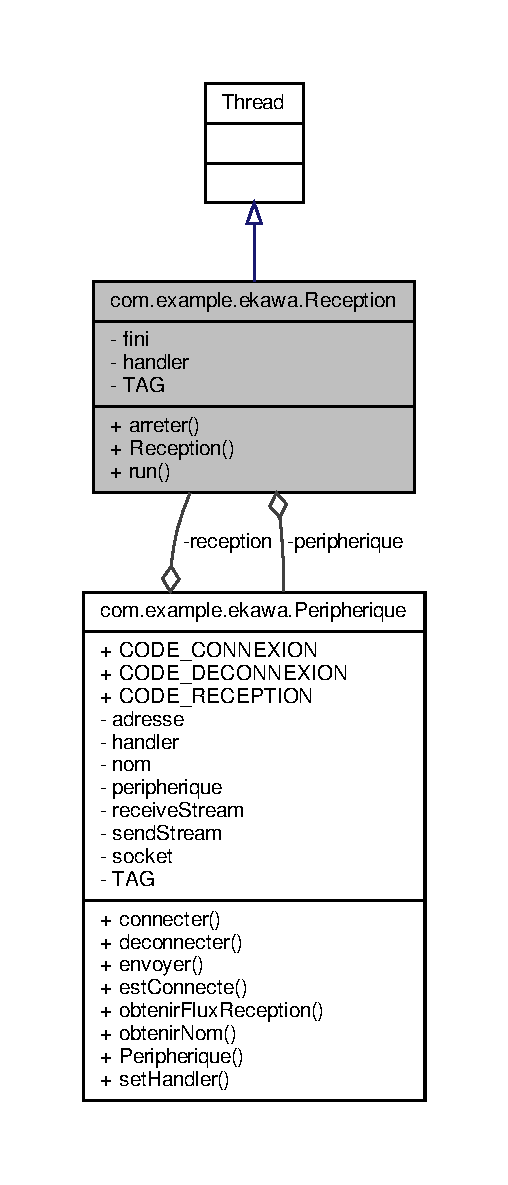
\includegraphics[height=550pt]{classcom_1_1example_1_1ekawa_1_1_reception__coll__graph}
\end{center}
\end{figure}
\subsubsection*{Fonctions membres publiques}
\begin{DoxyCompactItemize}
\item 
void \hyperlink{classcom_1_1example_1_1ekawa_1_1_reception_a844c65410aaeee936f6b0d44f9df56db}{arreter} ()
\begin{DoxyCompactList}\small\item\em Méthode qui permet d\textquotesingle{}arreter la réception de trame. \end{DoxyCompactList}\item 
\hyperlink{classcom_1_1example_1_1ekawa_1_1_reception_a82ddcbf05814957889ace3961d8cfde6}{Reception} (\hyperlink{classcom_1_1example_1_1ekawa_1_1_peripherique}{Peripherique} \hyperlink{classcom_1_1example_1_1ekawa_1_1_reception_a9f41511c4449d90da78017ca698367ef}{peripherique}, Handler \hyperlink{classcom_1_1example_1_1ekawa_1_1_reception_ab6273fbebb5aca17b9f95e275f1d3d38}{handler})
\begin{DoxyCompactList}\small\item\em Constructeur de la classe \hyperlink{classcom_1_1example_1_1ekawa_1_1_peripherique}{Peripherique}. \end{DoxyCompactList}\item 
void \hyperlink{classcom_1_1example_1_1ekawa_1_1_reception_ae5731cf974df539d32bfaded7b29d3c0}{run} ()
\begin{DoxyCompactList}\small\item\em Méthode qui permet de recevoir des trames de la cafetière (thread) \end{DoxyCompactList}\end{DoxyCompactItemize}
\subsubsection*{Attributs privés}
\begin{DoxyCompactItemize}
\item 
boolean \hyperlink{classcom_1_1example_1_1ekawa_1_1_reception_a10e50f0a5152056cf0c79c53bfa01cc9}{fini} = false
\item 
Handler \hyperlink{classcom_1_1example_1_1ekawa_1_1_reception_ab6273fbebb5aca17b9f95e275f1d3d38}{handler}
\item 
\hyperlink{classcom_1_1example_1_1ekawa_1_1_peripherique}{Peripherique} \hyperlink{classcom_1_1example_1_1ekawa_1_1_reception_a9f41511c4449d90da78017ca698367ef}{peripherique}
\end{DoxyCompactItemize}
\subsubsection*{Attributs privés statiques}
\begin{DoxyCompactItemize}
\item 
static final String \hyperlink{classcom_1_1example_1_1ekawa_1_1_reception_a4e155d4690591616f1064e17764df72b}{T\+AG} = \char`\"{}Reception\char`\"{}
\begin{DoxyCompactList}\small\item\em T\+AG pour les logs. \end{DoxyCompactList}\end{DoxyCompactItemize}


\subsubsection{Description détaillée}
Permet la réception des trames du périphérique Bluetooth de la cafetière. 

Définition à la ligne \hyperlink{_reception_8java_source_l00023}{23} du fichier \hyperlink{_reception_8java_source}{Reception.\+java}.



\subsubsection{Documentation des constructeurs et destructeur}
\mbox{\Hypertarget{classcom_1_1example_1_1ekawa_1_1_reception_a82ddcbf05814957889ace3961d8cfde6}\label{classcom_1_1example_1_1ekawa_1_1_reception_a82ddcbf05814957889ace3961d8cfde6}} 
\index{com\+::example\+::ekawa\+::\+Reception@{com\+::example\+::ekawa\+::\+Reception}!Reception@{Reception}}
\index{Reception@{Reception}!com\+::example\+::ekawa\+::\+Reception@{com\+::example\+::ekawa\+::\+Reception}}
\paragraph{\texorpdfstring{Reception()}{Reception()}}
{\footnotesize\ttfamily com.\+example.\+ekawa.\+Reception.\+Reception (\begin{DoxyParamCaption}\item[{\hyperlink{classcom_1_1example_1_1ekawa_1_1_peripherique}{Peripherique}}]{peripherique,  }\item[{Handler}]{handler }\end{DoxyParamCaption})}



Constructeur de la classe \hyperlink{classcom_1_1example_1_1ekawa_1_1_peripherique}{Peripherique}. 



Définition à la ligne \hyperlink{_reception_8java_source_l00033}{33} du fichier \hyperlink{_reception_8java_source}{Reception.\+java}.



Références \hyperlink{_reception_8java_source_l00027}{com.\+example.\+ekawa.\+Reception.\+handler}, et \hyperlink{_reception_8java_source_l00026}{com.\+example.\+ekawa.\+Reception.\+peripherique}.


\begin{DoxyCode}
00034     \{
00035         this.\hyperlink{classcom_1_1example_1_1ekawa_1_1_reception_a9f41511c4449d90da78017ca698367ef}{peripherique} = \hyperlink{classcom_1_1example_1_1ekawa_1_1_reception_a9f41511c4449d90da78017ca698367ef}{peripherique};
00036         this.\hyperlink{classcom_1_1example_1_1ekawa_1_1_reception_ab6273fbebb5aca17b9f95e275f1d3d38}{handler} = \hyperlink{classcom_1_1example_1_1ekawa_1_1_reception_ab6273fbebb5aca17b9f95e275f1d3d38}{handler};
00037     \}
\end{DoxyCode}


\subsubsection{Documentation des fonctions membres}
\mbox{\Hypertarget{classcom_1_1example_1_1ekawa_1_1_reception_a844c65410aaeee936f6b0d44f9df56db}\label{classcom_1_1example_1_1ekawa_1_1_reception_a844c65410aaeee936f6b0d44f9df56db}} 
\index{com\+::example\+::ekawa\+::\+Reception@{com\+::example\+::ekawa\+::\+Reception}!arreter@{arreter}}
\index{arreter@{arreter}!com\+::example\+::ekawa\+::\+Reception@{com\+::example\+::ekawa\+::\+Reception}}
\paragraph{\texorpdfstring{arreter()}{arreter()}}
{\footnotesize\ttfamily void com.\+example.\+ekawa.\+Reception.\+arreter (\begin{DoxyParamCaption}{ }\end{DoxyParamCaption})}



Méthode qui permet d\textquotesingle{}arreter la réception de trame. 



Définition à la ligne \hyperlink{_reception_8java_source_l00088}{88} du fichier \hyperlink{_reception_8java_source}{Reception.\+java}.



Référencé par \hyperlink{_peripherique_8java_source_l00150}{com.\+example.\+ekawa.\+Peripherique.\+deconnecter()}.


\begin{DoxyCode}
00089     \{
00090         \textcolor{keywordflow}{if} (\hyperlink{classcom_1_1example_1_1ekawa_1_1_reception_a10e50f0a5152056cf0c79c53bfa01cc9}{fini} == \textcolor{keyword}{false})
00091         \{
00092             \hyperlink{classcom_1_1example_1_1ekawa_1_1_reception_a10e50f0a5152056cf0c79c53bfa01cc9}{fini} = \textcolor{keyword}{true};
00093         \}
00094         \textcolor{keywordflow}{try}
00095         \{
00096             \hyperlink{class_thread}{Thread}.sleep(250);
00097         \}
00098         \textcolor{keywordflow}{catch} (InterruptedException e)
00099         \{
00100             e.printStackTrace();
00101         \}
00102     \}
\end{DoxyCode}
\mbox{\Hypertarget{classcom_1_1example_1_1ekawa_1_1_reception_ae5731cf974df539d32bfaded7b29d3c0}\label{classcom_1_1example_1_1ekawa_1_1_reception_ae5731cf974df539d32bfaded7b29d3c0}} 
\index{com\+::example\+::ekawa\+::\+Reception@{com\+::example\+::ekawa\+::\+Reception}!run@{run}}
\index{run@{run}!com\+::example\+::ekawa\+::\+Reception@{com\+::example\+::ekawa\+::\+Reception}}
\paragraph{\texorpdfstring{run()}{run()}}
{\footnotesize\ttfamily void com.\+example.\+ekawa.\+Reception.\+run (\begin{DoxyParamCaption}{ }\end{DoxyParamCaption})}



Méthode qui permet de recevoir des trames de la cafetière (thread) 



Définition à la ligne \hyperlink{_reception_8java_source_l00043}{43} du fichier \hyperlink{_reception_8java_source}{Reception.\+java}.



Références \hyperlink{_peripherique_8java_source_l00034}{com.\+example.\+ekawa.\+Peripherique.\+C\+O\+D\+E\+\_\+\+R\+E\+C\+E\+P\+T\+I\+ON}, et \hyperlink{_peripherique_8java_source_l00252}{com.\+example.\+ekawa.\+Peripherique.\+obtenir\+Flux\+Reception()}.


\begin{DoxyCode}
00044     \{
00045         Log.d(\hyperlink{classcom_1_1example_1_1ekawa_1_1_reception_a4e155d4690591616f1064e17764df72b}{TAG}, \textcolor{stringliteral}{"Thread réception démarré"});
00046         BufferedReader reception = \textcolor{keyword}{new} BufferedReader(\textcolor{keyword}{new} InputStreamReader(
      \hyperlink{classcom_1_1example_1_1ekawa_1_1_reception_a9f41511c4449d90da78017ca698367ef}{peripherique}.\hyperlink{classcom_1_1example_1_1ekawa_1_1_peripherique_a8b88d0a0d9e0c1b1aae04ba7c9d24619}{obtenirFluxReception}()));
00047         \textcolor{keywordflow}{while}(!\hyperlink{classcom_1_1example_1_1ekawa_1_1_reception_a10e50f0a5152056cf0c79c53bfa01cc9}{fini})
00048         \{
00049             \textcolor{keywordflow}{try}
00050             \{
00051                 String trame = \textcolor{stringliteral}{""};
00052                 \textcolor{keywordflow}{if}(reception.ready())
00053                 \{
00054                     trame = reception.readLine(); \textcolor{comment}{// Recupère la trame recue sans les délimiteurs de fin
       (\(\backslash\)r\(\backslash\)n)}
00055                 \}
00056                 \textcolor{keywordflow}{if}(trame.length() > 0)
00057                 \{
00058                     Log.d(\hyperlink{classcom_1_1example_1_1ekawa_1_1_reception_a4e155d4690591616f1064e17764df72b}{TAG}, \textcolor{stringliteral}{"run() trame : "} + trame);
00059                     \textcolor{keywordflow}{if}(\hyperlink{classcom_1_1example_1_1ekawa_1_1_reception_ab6273fbebb5aca17b9f95e275f1d3d38}{handler} != null)
00060                     \{
00061                         Message msg = Message.obtain();
00062                         msg.what = Peripherique.CODE\_RECEPTION;
00063                         msg.obj = trame;
00064                         \hyperlink{classcom_1_1example_1_1ekawa_1_1_reception_ab6273fbebb5aca17b9f95e275f1d3d38}{handler}.sendMessage(msg);
00065                     \}
00066                 \}
00067             \}
00068             \textcolor{keywordflow}{catch} (IOException e)
00069             \{
00070                 Log.d(\hyperlink{classcom_1_1example_1_1ekawa_1_1_reception_a4e155d4690591616f1064e17764df72b}{TAG}, \textcolor{stringliteral}{"Erreur lecture socket !"});
00071                  e.printStackTrace();
00072             \}
00073             \textcolor{keywordflow}{try}
00074             \{
00075                 \hyperlink{class_thread}{Thread}.sleep(250);
00076             \}
00077             \textcolor{keywordflow}{catch} (InterruptedException e)
00078             \{
00079                 e.printStackTrace();
00080             \}
00081         \}
00082         Log.d(\hyperlink{classcom_1_1example_1_1ekawa_1_1_reception_a4e155d4690591616f1064e17764df72b}{TAG}, \textcolor{stringliteral}{"Thread réception arrêté"});
00083     \}
\end{DoxyCode}


\subsubsection{Documentation des données membres}
\mbox{\Hypertarget{classcom_1_1example_1_1ekawa_1_1_reception_a10e50f0a5152056cf0c79c53bfa01cc9}\label{classcom_1_1example_1_1ekawa_1_1_reception_a10e50f0a5152056cf0c79c53bfa01cc9}} 
\index{com\+::example\+::ekawa\+::\+Reception@{com\+::example\+::ekawa\+::\+Reception}!fini@{fini}}
\index{fini@{fini}!com\+::example\+::ekawa\+::\+Reception@{com\+::example\+::ekawa\+::\+Reception}}
\paragraph{\texorpdfstring{fini}{fini}}
{\footnotesize\ttfamily boolean com.\+example.\+ekawa.\+Reception.\+fini = false\hspace{0.3cm}{\ttfamily [private]}}



Définition à la ligne \hyperlink{_reception_8java_source_l00028}{28} du fichier \hyperlink{_reception_8java_source}{Reception.\+java}.

\mbox{\Hypertarget{classcom_1_1example_1_1ekawa_1_1_reception_ab6273fbebb5aca17b9f95e275f1d3d38}\label{classcom_1_1example_1_1ekawa_1_1_reception_ab6273fbebb5aca17b9f95e275f1d3d38}} 
\index{com\+::example\+::ekawa\+::\+Reception@{com\+::example\+::ekawa\+::\+Reception}!handler@{handler}}
\index{handler@{handler}!com\+::example\+::ekawa\+::\+Reception@{com\+::example\+::ekawa\+::\+Reception}}
\paragraph{\texorpdfstring{handler}{handler}}
{\footnotesize\ttfamily Handler com.\+example.\+ekawa.\+Reception.\+handler\hspace{0.3cm}{\ttfamily [private]}}



Définition à la ligne \hyperlink{_reception_8java_source_l00027}{27} du fichier \hyperlink{_reception_8java_source}{Reception.\+java}.



Référencé par \hyperlink{_reception_8java_source_l00033}{com.\+example.\+ekawa.\+Reception.\+Reception()}.

\mbox{\Hypertarget{classcom_1_1example_1_1ekawa_1_1_reception_a9f41511c4449d90da78017ca698367ef}\label{classcom_1_1example_1_1ekawa_1_1_reception_a9f41511c4449d90da78017ca698367ef}} 
\index{com\+::example\+::ekawa\+::\+Reception@{com\+::example\+::ekawa\+::\+Reception}!peripherique@{peripherique}}
\index{peripherique@{peripherique}!com\+::example\+::ekawa\+::\+Reception@{com\+::example\+::ekawa\+::\+Reception}}
\paragraph{\texorpdfstring{peripherique}{peripherique}}
{\footnotesize\ttfamily \hyperlink{classcom_1_1example_1_1ekawa_1_1_peripherique}{Peripherique} com.\+example.\+ekawa.\+Reception.\+peripherique\hspace{0.3cm}{\ttfamily [private]}}



Définition à la ligne \hyperlink{_reception_8java_source_l00026}{26} du fichier \hyperlink{_reception_8java_source}{Reception.\+java}.



Référencé par \hyperlink{_reception_8java_source_l00033}{com.\+example.\+ekawa.\+Reception.\+Reception()}.

\mbox{\Hypertarget{classcom_1_1example_1_1ekawa_1_1_reception_a4e155d4690591616f1064e17764df72b}\label{classcom_1_1example_1_1ekawa_1_1_reception_a4e155d4690591616f1064e17764df72b}} 
\index{com\+::example\+::ekawa\+::\+Reception@{com\+::example\+::ekawa\+::\+Reception}!T\+AG@{T\+AG}}
\index{T\+AG@{T\+AG}!com\+::example\+::ekawa\+::\+Reception@{com\+::example\+::ekawa\+::\+Reception}}
\paragraph{\texorpdfstring{T\+AG}{TAG}}
{\footnotesize\ttfamily final String com.\+example.\+ekawa.\+Reception.\+T\+AG = \char`\"{}Reception\char`\"{}\hspace{0.3cm}{\ttfamily [static]}, {\ttfamily [private]}}



T\+AG pour les logs. 



Définition à la ligne \hyperlink{_reception_8java_source_l00025}{25} du fichier \hyperlink{_reception_8java_source}{Reception.\+java}.



La documentation de cette classe a été générée à partir du fichier suivant \+:\begin{DoxyCompactItemize}
\item 
\hyperlink{_reception_8java}{Reception.\+java}\end{DoxyCompactItemize}

\hypertarget{class_thread}{}\subsection{Référence de la classe Thread}
\label{class_thread}\index{Thread@{Thread}}


Graphe de collaboration de Thread\+:\nopagebreak
\begin{figure}[H]
\begin{center}
\leavevmode
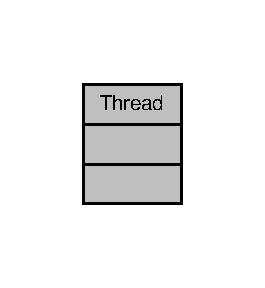
\includegraphics[width=127pt]{class_thread__coll__graph}
\end{center}
\end{figure}


La documentation de cette classe a été générée à partir du fichier suivant \+:\begin{DoxyCompactItemize}
\item 
\hyperlink{_reception_8java}{Reception.\+java}\end{DoxyCompactItemize}

\section{Documentation des fichiers}
\hypertarget{_boisson_8java}{}\subsection{Référence du fichier Boisson.\+java}
\label{_boisson_8java}\index{Boisson.\+java@{Boisson.\+java}}


Déclaration de la classe Boisson.  


\subsubsection*{Classes}
\begin{DoxyCompactItemize}
\item 
class \hyperlink{classcom_1_1example_1_1ekawa_1_1_boisson}{com.\+example.\+ekawa.\+Boisson}
\begin{DoxyCompactList}\small\item\em Définit les caractéristiques des boissons d\textquotesingle{}E\+K\+A\+WA. \end{DoxyCompactList}\end{DoxyCompactItemize}
\subsubsection*{Paquetages}
\begin{DoxyCompactItemize}
\item 
package \hyperlink{namespacecom_1_1example_1_1ekawa}{com.\+example.\+ekawa}
\end{DoxyCompactItemize}


\subsubsection{Description détaillée}
Déclaration de la classe Boisson. 

\begin{DoxyAuthor}{Auteur}
Jean-\/\+Luc Lecomte 
\end{DoxyAuthor}
\begin{DoxyParagraph}{Last\+Changed\+Revision}
76 
\end{DoxyParagraph}
\begin{DoxyParagraph}{Last\+Changed\+Date}
2021-\/04-\/27 21\+:54\+:24 +0200 (mar. 27 avril 2021) 
\end{DoxyParagraph}


Définition dans le fichier \hyperlink{_boisson_8java_source}{Boisson.\+java}.


\hypertarget{_boisson_8java_source}{}\subsection{Boisson.\+java}
\label{_boisson_8java_source}\index{Boisson.\+java@{Boisson.\+java}}

\begin{DoxyCode}
\Hypertarget{_boisson_8java_source_l00001}\hyperlink{namespacecom_1_1example_1_1ekawa}{00001} \textcolor{keyword}{package }com.example.ekawa;
00002 
\Hypertarget{_boisson_8java_source_l00015}\hyperlink{classcom_1_1example_1_1ekawa_1_1_boisson}{00015} \textcolor{keyword}{public} \textcolor{keyword}{class }\hyperlink{classcom_1_1example_1_1ekawa_1_1_boisson}{Boisson}
00016 \{
\Hypertarget{_boisson_8java_source_l00017}\hyperlink{classcom_1_1example_1_1ekawa_1_1_boisson_a9c932ca6665790c36acb6d4792a5a31a}{00017}     \textcolor{keyword}{private} String \hyperlink{classcom_1_1example_1_1ekawa_1_1_boisson_a9c932ca6665790c36acb6d4792a5a31a}{nom};
\Hypertarget{_boisson_8java_source_l00018}\hyperlink{classcom_1_1example_1_1ekawa_1_1_boisson_ac73d259d39e459b00e5cfdf73a2aaf98}{00018}     \textcolor{keyword}{private} Integer \hyperlink{classcom_1_1example_1_1ekawa_1_1_boisson_ac73d259d39e459b00e5cfdf73a2aaf98}{identifiantImage};
00019 
\Hypertarget{_boisson_8java_source_l00025}\hyperlink{classcom_1_1example_1_1ekawa_1_1_boisson_a4dd8019f54eb6d1293a179ffe5e8b918}{00025}     \textcolor{keyword}{public} \hyperlink{classcom_1_1example_1_1ekawa_1_1_boisson_a4dd8019f54eb6d1293a179ffe5e8b918}{Boisson}(String nom, Integer identifiantImage)
00026     \{
00027         this.nom = \hyperlink{classcom_1_1example_1_1ekawa_1_1_boisson_a9c932ca6665790c36acb6d4792a5a31a}{nom};
00028         this.identifiantImage = \hyperlink{classcom_1_1example_1_1ekawa_1_1_boisson_ac73d259d39e459b00e5cfdf73a2aaf98}{identifiantImage};
00029     \}
00030 
\Hypertarget{_boisson_8java_source_l00035}\hyperlink{classcom_1_1example_1_1ekawa_1_1_boisson_a410781851622f3c4b87a30d7381f9082}{00035}     \textcolor{keyword}{public} String \hyperlink{classcom_1_1example_1_1ekawa_1_1_boisson_a410781851622f3c4b87a30d7381f9082}{obtenirNom}()
00036     \{
00037         \textcolor{keywordflow}{return} this.\hyperlink{classcom_1_1example_1_1ekawa_1_1_boisson_a9c932ca6665790c36acb6d4792a5a31a}{nom};
00038     \}
00039 
\Hypertarget{_boisson_8java_source_l00044}\hyperlink{classcom_1_1example_1_1ekawa_1_1_boisson_a6edf9114dd70c1c16382136e57e6d345}{00044}     \textcolor{keyword}{public} Integer \hyperlink{classcom_1_1example_1_1ekawa_1_1_boisson_a6edf9114dd70c1c16382136e57e6d345}{obtenirImage}()
00045     \{
00046         \textcolor{keywordflow}{return} this.\hyperlink{classcom_1_1example_1_1ekawa_1_1_boisson_ac73d259d39e459b00e5cfdf73a2aaf98}{identifiantImage};
00047     \}
00048 \}
\end{DoxyCode}

\hypertarget{_cafetiere_8java}{}\subsection{Référence du fichier Cafetiere.\+java}
\label{_cafetiere_8java}\index{Cafetiere.\+java@{Cafetiere.\+java}}


Déclaration de la classe Cafetiere.  


\subsubsection*{Classes}
\begin{DoxyCompactItemize}
\item 
class \hyperlink{classcom_1_1example_1_1ekawa_1_1_cafetiere}{com.\+example.\+ekawa.\+Cafetiere}
\begin{DoxyCompactList}\small\item\em Déclaration de la classe principale de l\textquotesingle{}application. \end{DoxyCompactList}\end{DoxyCompactItemize}
\subsubsection*{Paquetages}
\begin{DoxyCompactItemize}
\item 
package \hyperlink{namespacecom_1_1example_1_1ekawa}{com.\+example.\+ekawa}
\end{DoxyCompactItemize}


\subsubsection{Description détaillée}
Déclaration de la classe Cafetiere. 

\begin{DoxyAuthor}{Auteur}
Jean-\/\+Luc Lecomte 
\end{DoxyAuthor}
\begin{DoxyParagraph}{Last\+Changed\+Revision}
76 
\end{DoxyParagraph}
\begin{DoxyParagraph}{Last\+Changed\+Date}
2021-\/04-\/27 21\+:54\+:24 +0200 (mar. 27 avril 2021) 
\end{DoxyParagraph}


Définition dans le fichier \hyperlink{_cafetiere_8java_source}{Cafetiere.\+java}.


\hypertarget{_cafetiere_8java_source}{}\subsection{Cafetiere.\+java}
\label{_cafetiere_8java_source}\index{Cafetiere.\+java@{Cafetiere.\+java}}

\begin{DoxyCode}
00001 \textcolor{keyword}{package }com.example.ekawa;
00002 
00003 \textcolor{keyword}{import} android.util.Log;
00004 
00005 \textcolor{keyword}{import} android.widget.Toast;
00006 
00007 \textcolor{keyword}{import} java.lang.reflect.ParameterizedType;
00008 \textcolor{keyword}{import} java.util.ArrayList;
00009 
\Hypertarget{_cafetiere_8java_source_l00022}\hyperlink{classcom_1_1example_1_1ekawa_1_1_cafetiere}{00022} \textcolor{keyword}{public} \textcolor{keyword}{class }\hyperlink{classcom_1_1example_1_1ekawa_1_1_cafetiere}{Cafetiere}
00023 \{
\Hypertarget{_cafetiere_8java_source_l00027}\hyperlink{classcom_1_1example_1_1ekawa_1_1_cafetiere_aa0c1fd99a2508b06c462aea17034aa91}{00027}     \textcolor{keyword}{private} \textcolor{keyword}{static} \textcolor{keyword}{final} String \hyperlink{classcom_1_1example_1_1ekawa_1_1_cafetiere_aa0c1fd99a2508b06c462aea17034aa91}{TAG} = \textcolor{stringliteral}{"Cafetiere"};          
\Hypertarget{_cafetiere_8java_source_l00028}\hyperlink{classcom_1_1example_1_1ekawa_1_1_cafetiere_a5a23a636fa5f2e5826458e700f453c16}{00028}     \textcolor{keyword}{public} \textcolor{keyword}{static} \textcolor{keyword}{final} \textcolor{keywordtype}{int} \hyperlink{classcom_1_1example_1_1ekawa_1_1_cafetiere_a5a23a636fa5f2e5826458e700f453c16}{AUCUNE\_CAPSULE} = -1;            
\Hypertarget{_cafetiere_8java_source_l00029}\hyperlink{classcom_1_1example_1_1ekawa_1_1_cafetiere_a183d96e89c056c4ac9c565bf8f24851e}{00029}     \textcolor{keyword}{public} \textcolor{keyword}{static} \textcolor{keyword}{final} Integer \hyperlink{classcom_1_1example_1_1ekawa_1_1_cafetiere_a183d96e89c056c4ac9c565bf8f24851e}{NOMBRE\_CAPSULE\_MAX} = 8;     
\Hypertarget{_cafetiere_8java_source_l00030}\hyperlink{classcom_1_1example_1_1ekawa_1_1_cafetiere_a2be5950bf3bb155b8396593d390b808b}{00030}     \textcolor{keyword}{public} \textcolor{keyword}{static} \textcolor{keyword}{final} Integer \hyperlink{classcom_1_1example_1_1ekawa_1_1_cafetiere_a2be5950bf3bb155b8396593d390b808b}{NOMBRE\_BOISSON\_MAX} = 2;     
\Hypertarget{_cafetiere_8java_source_l00031}\hyperlink{classcom_1_1example_1_1ekawa_1_1_cafetiere_a9e0cce07580820dfbc85696f1fb82aef}{00031}     \textcolor{keyword}{public} \textcolor{keyword}{final} \textcolor{keyword}{static} \textcolor{keywordtype}{int} \hyperlink{classcom_1_1example_1_1ekawa_1_1_cafetiere_a9e0cce07580820dfbc85696f1fb82aef}{NB\_MAX\_CAFE\_CONSEILLEE} = 4;     
\Hypertarget{_cafetiere_8java_source_l00032}\hyperlink{classcom_1_1example_1_1ekawa_1_1_cafetiere_a5b10663105c7e3fd28dfd9d51b5e925f}{00032}     \textcolor{keyword}{public} \textcolor{keyword}{final} \textcolor{keyword}{static} String \hyperlink{classcom_1_1example_1_1ekawa_1_1_cafetiere_a5b10663105c7e3fd28dfd9d51b5e925f}{NOM\_CAFETIERE\_NON\_CONNECTEE} = \textcolor{stringliteral}{"Aucune"}; 
00033 
\Hypertarget{_cafetiere_8java_source_l00037}\hyperlink{classcom_1_1example_1_1ekawa_1_1_cafetiere_a127a27c8f3b4c6c5dc4bfb639f654b3d}{00037}     \textcolor{keyword}{private} String[] \hyperlink{classcom_1_1example_1_1ekawa_1_1_cafetiere_a127a27c8f3b4c6c5dc4bfb639f654b3d}{nomsCapusles} = \{
00038             \textcolor{stringliteral}{"Colombia"},
00039             \textcolor{stringliteral}{"Indonesia"},
00040             \textcolor{stringliteral}{"Ethiopia"},
00041             \textcolor{stringliteral}{"Volluto"},
00042             \textcolor{stringliteral}{"Capriccio"},
00043             \textcolor{stringliteral}{"Cosi"},
00044             \textcolor{stringliteral}{"Scuro"},
00045             \textcolor{stringliteral}{"Vanilla Eclair"}
00046     \}; 
00047 
\Hypertarget{_cafetiere_8java_source_l00048}\hyperlink{classcom_1_1example_1_1ekawa_1_1_cafetiere_a7558b3f423bd53d4198a7c143bd2d657}{00048}     \textcolor{keyword}{private} Integer[] \hyperlink{classcom_1_1example_1_1ekawa_1_1_cafetiere_a7558b3f423bd53d4198a7c143bd2d657}{idImagesCapsules} =
00049     \{
00050             R.mipmap.ic\_capsule\_colombia,
00051             R.mipmap.ic\_capsule\_indonesia,
00052             R.mipmap.ic\_capsule\_ethiopia,
00053             R.mipmap.ic\_capsule\_volluto,
00054             R.mipmap.ic\_capsule\_capriccio,
00055             R.mipmap.ic\_capsule\_cosi,
00056             R.mipmap.ic\_capsule\_scuro,
00057             R.mipmap.ic\_capsule\_vanilla\_eclair
00058     \};
00059 
\Hypertarget{_cafetiere_8java_source_l00060}\hyperlink{classcom_1_1example_1_1ekawa_1_1_cafetiere_aebaaf300362a258e047ae31b7e56e622}{00060}     \textcolor{keyword}{private} \textcolor{keywordtype}{boolean}[] \hyperlink{classcom_1_1example_1_1ekawa_1_1_cafetiere_aebaaf300362a258e047ae31b7e56e622}{presencesCapsules} = \{ \textcolor{keyword}{true}, \textcolor{keyword}{true}, \textcolor{keyword}{true}, \textcolor{keyword}{true}, \textcolor{keyword}{true}, \textcolor{keyword}{true}, \textcolor{keyword}{true}, \textcolor{keyword}{true}
       \};
00061 
\Hypertarget{_cafetiere_8java_source_l00062}\hyperlink{classcom_1_1example_1_1ekawa_1_1_cafetiere_a59db420b33a9f03aad97d6cad4f87c03}{00062}     \textcolor{keyword}{private} String[] \hyperlink{classcom_1_1example_1_1ekawa_1_1_cafetiere_a59db420b33a9f03aad97d6cad4f87c03}{nomsBoissons} = \{ \textcolor{stringliteral}{"Court"}, \textcolor{stringliteral}{"Long"} \};
00063 
\Hypertarget{_cafetiere_8java_source_l00064}\hyperlink{classcom_1_1example_1_1ekawa_1_1_cafetiere_a10645115a166d3529e63aeb4ea16a869}{00064}     \textcolor{keyword}{private} Integer[] \hyperlink{classcom_1_1example_1_1ekawa_1_1_cafetiere_a10645115a166d3529e63aeb4ea16a869}{idImagesBoissons} = \{ R.drawable.ic\_cafe\_court, R.drawable.
      ic\_cafe\_long \};
00065 
\Hypertarget{_cafetiere_8java_source_l00066}\hyperlink{classcom_1_1example_1_1ekawa_1_1_cafetiere_a054b6a7668e317cfa1da3d8600311e4e}{00066}     \textcolor{keyword}{private} Integer[] \hyperlink{classcom_1_1example_1_1ekawa_1_1_cafetiere_a054b6a7668e317cfa1da3d8600311e4e}{descriptionCapsules} = \{
00067             R.string.colombia,
00068             R.string.indonesia,
00069             R.string.ethiopia,
00070             R.string.volluto,
00071             R.string.capriccio,
00072             R.string.cosi,
00073             R.string.scuro,
00074             R.string.vanilla\_eclair
00075     \};
00076 
\Hypertarget{_cafetiere_8java_source_l00077}\hyperlink{classcom_1_1example_1_1ekawa_1_1_cafetiere_ae5fa359f1ddcbd80ce3651e2d7368ff8}{00077}     \textcolor{keyword}{private} \hyperlink{classcom_1_1example_1_1ekawa_1_1_programmation}{Programmation} \hyperlink{classcom_1_1example_1_1ekawa_1_1_cafetiere_ae5fa359f1ddcbd80ce3651e2d7368ff8}{derniereProgrammation};
\Hypertarget{_cafetiere_8java_source_l00078}\hyperlink{classcom_1_1example_1_1ekawa_1_1_cafetiere_a79faede6506425563ec617affef48e09}{00078}     \textcolor{keyword}{private} \textcolor{keywordtype}{int} \hyperlink{classcom_1_1example_1_1ekawa_1_1_cafetiere_a79faede6506425563ec617affef48e09}{derniereSuppressionProgrammation};
00079 
\Hypertarget{_cafetiere_8java_source_l00080}\hyperlink{classcom_1_1example_1_1ekawa_1_1_cafetiere_a7db4a63088834eda5f6a3e951611bf82}{00080}     \textcolor{keyword}{private} \hyperlink{classcom_1_1example_1_1ekawa_1_1_ihm}{Ihm} \hyperlink{classcom_1_1example_1_1ekawa_1_1_cafetiere_a7db4a63088834eda5f6a3e951611bf82}{ihm};
\Hypertarget{_cafetiere_8java_source_l00081}\hyperlink{classcom_1_1example_1_1ekawa_1_1_cafetiere_af9506a7805d000d2cb83444cdb8ea889}{00081}     \textcolor{keyword}{private} \hyperlink{classcom_1_1example_1_1ekawa_1_1_communication}{Communication} \hyperlink{classcom_1_1example_1_1ekawa_1_1_cafetiere_af9506a7805d000d2cb83444cdb8ea889}{communication} = null;
\Hypertarget{_cafetiere_8java_source_l00082}\hyperlink{classcom_1_1example_1_1ekawa_1_1_cafetiere_aee3f9b78df63bc8dd73bf564954d51ca}{00082}     \textcolor{keyword}{private} \hyperlink{classcom_1_1example_1_1ekawa_1_1_preference}{Preference} \hyperlink{classcom_1_1example_1_1ekawa_1_1_cafetiere_aee3f9b78df63bc8dd73bf564954d51ca}{preference} = null;
\Hypertarget{_cafetiere_8java_source_l00083}\hyperlink{classcom_1_1example_1_1ekawa_1_1_cafetiere_a987c8e1bcea506b65f4b05f955b3f699}{00083}     \textcolor{keyword}{private} ArrayList<Programmation> \hyperlink{classcom_1_1example_1_1ekawa_1_1_cafetiere_a987c8e1bcea506b65f4b05f955b3f699}{programmations};
00084 
\Hypertarget{_cafetiere_8java_source_l00085}\hyperlink{classcom_1_1example_1_1ekawa_1_1_cafetiere_ae9590789503a6ae2094c86cf93299821}{00085}     \textcolor{keyword}{private} ArrayList<Capsule> \hyperlink{classcom_1_1example_1_1ekawa_1_1_cafetiere_ae9590789503a6ae2094c86cf93299821}{capsules};
\Hypertarget{_cafetiere_8java_source_l00086}\hyperlink{classcom_1_1example_1_1ekawa_1_1_cafetiere_aad375efbc01f1db83572f4ae567189de}{00086}     \textcolor{keyword}{private} ArrayList<Boisson> \hyperlink{classcom_1_1example_1_1ekawa_1_1_cafetiere_aad375efbc01f1db83572f4ae567189de}{boissons};
\Hypertarget{_cafetiere_8java_source_l00087}\hyperlink{classcom_1_1example_1_1ekawa_1_1_cafetiere_ac8fa3d1ad76eccf431ee04b395a557a3}{00087}     \textcolor{keyword}{private} \textcolor{keywordtype}{int} \hyperlink{classcom_1_1example_1_1ekawa_1_1_cafetiere_ac8fa3d1ad76eccf431ee04b395a557a3}{capsuleActuelle} = \hyperlink{classcom_1_1example_1_1ekawa_1_1_cafetiere_a5a23a636fa5f2e5826458e700f453c16}{AUCUNE\_CAPSULE};
\Hypertarget{_cafetiere_8java_source_l00088}\hyperlink{classcom_1_1example_1_1ekawa_1_1_cafetiere_a73c5fa3b510655e1e3425140336b7f5b}{00088}     \textcolor{keyword}{private} \textcolor{keywordtype}{int} \hyperlink{classcom_1_1example_1_1ekawa_1_1_cafetiere_a73c5fa3b510655e1e3425140336b7f5b}{boissonActuelle} = 0;
00089 
\Hypertarget{_cafetiere_8java_source_l00090}\hyperlink{classcom_1_1example_1_1ekawa_1_1_cafetiere_ae170dd018d1e740b3bda080d1cc3d900}{00090}     \textcolor{keyword}{private} \textcolor{keywordtype}{boolean} \hyperlink{classcom_1_1example_1_1ekawa_1_1_cafetiere_ae170dd018d1e740b3bda080d1cc3d900}{etatCafetiere} = \textcolor{keyword}{false};
\Hypertarget{_cafetiere_8java_source_l00091}\hyperlink{classcom_1_1example_1_1ekawa_1_1_cafetiere_a93c5021591facf06397e760c11556904}{00091}     \textcolor{keyword}{private} \textcolor{keywordtype}{boolean} \hyperlink{classcom_1_1example_1_1ekawa_1_1_cafetiere_a93c5021591facf06397e760c11556904}{etatTasse} = \textcolor{keyword}{false};
\Hypertarget{_cafetiere_8java_source_l00092}\hyperlink{classcom_1_1example_1_1ekawa_1_1_cafetiere_a058f7a18cd9c0567d583b8bc6250d143}{00092}     \textcolor{keyword}{private} \textcolor{keywordtype}{boolean} \hyperlink{classcom_1_1example_1_1ekawa_1_1_cafetiere_a058f7a18cd9c0567d583b8bc6250d143}{etatBac} = \textcolor{keyword}{false};
\Hypertarget{_cafetiere_8java_source_l00093}\hyperlink{classcom_1_1example_1_1ekawa_1_1_cafetiere_aaf8e1a960f803c2de4defa414b5984a4}{00093}     \textcolor{keyword}{private} \textcolor{keywordtype}{int} \hyperlink{classcom_1_1example_1_1ekawa_1_1_cafetiere_aaf8e1a960f803c2de4defa414b5984a4}{niveauEau} = 0;
00094 
00095 
\Hypertarget{_cafetiere_8java_source_l00096}\hyperlink{classcom_1_1example_1_1ekawa_1_1_cafetiere_a123b6fcb9a9c1decae40e026660e716b}{00096}     \textcolor{keyword}{private} \textcolor{keywordtype}{int} \hyperlink{classcom_1_1example_1_1ekawa_1_1_cafetiere_a123b6fcb9a9c1decae40e026660e716b}{nombreCafeDuJour} = 0; 
\Hypertarget{_cafetiere_8java_source_l00097}\hyperlink{classcom_1_1example_1_1ekawa_1_1_cafetiere_a61e4ab1e5ebdc60ffea39a344711e477}{00097}     \textcolor{keyword}{private} String \hyperlink{classcom_1_1example_1_1ekawa_1_1_cafetiere_a61e4ab1e5ebdc60ffea39a344711e477}{date} = null;
\Hypertarget{_cafetiere_8java_source_l00098}\hyperlink{classcom_1_1example_1_1ekawa_1_1_cafetiere_ac22f9da8ed59c7362871b8f22e501e23}{00098}     \textcolor{keyword}{private} \textcolor{keywordtype}{int} \hyperlink{classcom_1_1example_1_1ekawa_1_1_cafetiere_ac22f9da8ed59c7362871b8f22e501e23}{nombreCafeTotal} = 0; 
\Hypertarget{_cafetiere_8java_source_l00099}\hyperlink{classcom_1_1example_1_1ekawa_1_1_cafetiere_a6491d6d04db5d6e7da868565b84f6d7f}{00099}     \textcolor{keyword}{private} \textcolor{keywordtype}{int} \hyperlink{classcom_1_1example_1_1ekawa_1_1_cafetiere_a6491d6d04db5d6e7da868565b84f6d7f}{nombreBacVide} = 0;
\Hypertarget{_cafetiere_8java_source_l00100}\hyperlink{classcom_1_1example_1_1ekawa_1_1_cafetiere_a2332c2e33acff5084b4571663b48bd89}{00100}     \textcolor{keyword}{private} \textcolor{keywordtype}{int} \hyperlink{classcom_1_1example_1_1ekawa_1_1_cafetiere_a2332c2e33acff5084b4571663b48bd89}{nombreEauRemplie} = 0;
\Hypertarget{_cafetiere_8java_source_l00101}\hyperlink{classcom_1_1example_1_1ekawa_1_1_cafetiere_aafc365a43172fca9166fb2a9006c6ecf}{00101}     \textcolor{keyword}{private} \textcolor{keywordtype}{int} \hyperlink{classcom_1_1example_1_1ekawa_1_1_cafetiere_aafc365a43172fca9166fb2a9006c6ecf}{dureteeEau} = 0;
\Hypertarget{_cafetiere_8java_source_l00102}\hyperlink{classcom_1_1example_1_1ekawa_1_1_cafetiere_a27aba2ce49934d0bf7b2d2230b3003d7}{00102}     \textcolor{keyword}{private} \textcolor{keywordtype}{int} \hyperlink{classcom_1_1example_1_1ekawa_1_1_cafetiere_a27aba2ce49934d0bf7b2d2230b3003d7}{qualiteeEau} = 0;
00103 
\Hypertarget{_cafetiere_8java_source_l00108}\hyperlink{classcom_1_1example_1_1ekawa_1_1_cafetiere_a8a8b762148526c605b13daeaf9d2e7cb}{00108}     \textcolor{keyword}{public} \hyperlink{classcom_1_1example_1_1ekawa_1_1_cafetiere_a8a8b762148526c605b13daeaf9d2e7cb}{Cafetiere}(\hyperlink{classcom_1_1example_1_1ekawa_1_1_ihm}{Ihm} ihm)
00109     \{
00110         Log.d(TAG, \textcolor{stringliteral}{"Cafetiere()"});
00111         this.ihm = \hyperlink{classcom_1_1example_1_1ekawa_1_1_cafetiere_a7db4a63088834eda5f6a3e951611bf82}{ihm};
00112         \hyperlink{classcom_1_1example_1_1ekawa_1_1_cafetiere_a20f3b74112d4e668a382882c4c8ccd07}{initialiserPreference}();
00113         \hyperlink{classcom_1_1example_1_1ekawa_1_1_cafetiere_a75d0df422427eed8b12e7b46a6e11a35}{initialiserCapsules}();
00114         \hyperlink{classcom_1_1example_1_1ekawa_1_1_cafetiere_ae9092a9540897e60c4cf7307073a75ab}{initialiserBoissons}();
00115         \hyperlink{classcom_1_1example_1_1ekawa_1_1_cafetiere_ad7c3e155b2ddf4dae05da8cd9c38518a}{initialiserCommunication}();
00116         \hyperlink{classcom_1_1example_1_1ekawa_1_1_cafetiere_aae065b86cdb3a8df2c904068aab7e9bf}{initaliserProgrammation}();
00117     \}
00118 
\Hypertarget{_cafetiere_8java_source_l00122}\hyperlink{classcom_1_1example_1_1ekawa_1_1_cafetiere_a20f3b74112d4e668a382882c4c8ccd07}{00122}     \textcolor{keyword}{private} \textcolor{keywordtype}{void} \hyperlink{classcom_1_1example_1_1ekawa_1_1_cafetiere_a20f3b74112d4e668a382882c4c8ccd07}{initialiserPreference}()
00123     \{
00124         preference = \textcolor{keyword}{new} \hyperlink{classcom_1_1example_1_1ekawa_1_1_preference}{Preference}(ihm);
00125         \textcolor{comment}{//if(preference.contient(Preference.CAPSULE))}
00126         String donnee = preference.\hyperlink{classcom_1_1example_1_1ekawa_1_1_preference_a485d7fe31708aa1b85c0e2dcdcc05c0d}{obtenir}(\hyperlink{classcom_1_1example_1_1ekawa_1_1_preference}{Preference}.\hyperlink{classcom_1_1example_1_1ekawa_1_1_preference_a64416823eba6f35e817636b31cb12265}{CAPSULE}).toString();
00127         \textcolor{keywordflow}{if}(!donnee.isEmpty())
00128             capsuleActuelle = Integer.valueOf(donnee);
00129         \textcolor{keywordflow}{else}
00130             capsuleActuelle = 0; \textcolor{comment}{// première capsule}
00131         \textcolor{comment}{//if(preference.contient(Preference.CAPSULE))}
00132         donnee = preference.\hyperlink{classcom_1_1example_1_1ekawa_1_1_preference_a485d7fe31708aa1b85c0e2dcdcc05c0d}{obtenir}(\hyperlink{classcom_1_1example_1_1ekawa_1_1_preference}{Preference}.\hyperlink{classcom_1_1example_1_1ekawa_1_1_preference_a6923224bd12c5b50259e5f376ed58a35}{BOISSON}).toString();
00133         \textcolor{keywordflow}{if}(!donnee.isEmpty())
00134             boissonActuelle = Integer.valueOf(donnee);
00135         \textcolor{keywordflow}{else}
00136             boissonActuelle = 0; \textcolor{comment}{// café court}
00137         nombreCafeDuJour = preference.\hyperlink{classcom_1_1example_1_1ekawa_1_1_preference_a5a8f4c9f845924a0ebb3aec5ca99a5f5}{obtenirNombreCafeDuJour}(date, nombreCafeDuJour
      );
00138         Log.d(TAG, \textcolor{stringliteral}{"initialiserPreference() capsuleActuelle = "} + capsuleActuelle);
00139         Log.d(TAG, \textcolor{stringliteral}{"initialiserPreference() boissonActuelle = "} + boissonActuelle);
00140         Log.d(TAG, \textcolor{stringliteral}{"initialiserPreference() nombreCafeDuJour = "} + nombreCafeDuJour);
00141     \}
00142 
\Hypertarget{_cafetiere_8java_source_l00143}\hyperlink{classcom_1_1example_1_1ekawa_1_1_cafetiere_aae065b86cdb3a8df2c904068aab7e9bf}{00143}     \textcolor{keyword}{private} \textcolor{keywordtype}{void} \hyperlink{classcom_1_1example_1_1ekawa_1_1_cafetiere_aae065b86cdb3a8df2c904068aab7e9bf}{initaliserProgrammation}()
00144     \{
00145         Log.d(TAG, \textcolor{stringliteral}{"initaliserProgrammation()"});
00146         programmations = \textcolor{keyword}{new} ArrayList<Programmation>();
00147         \hyperlink{classcom_1_1example_1_1ekawa_1_1_cafetiere_a406e5771edb1663ebb1fc571365b75ac}{initialiserProgrammations}();
00148     \}
00149 
\Hypertarget{_cafetiere_8java_source_l00153}\hyperlink{classcom_1_1example_1_1ekawa_1_1_cafetiere_ad7c3e155b2ddf4dae05da8cd9c38518a}{00153}     \textcolor{keyword}{private} \textcolor{keywordtype}{void} \hyperlink{classcom_1_1example_1_1ekawa_1_1_cafetiere_ad7c3e155b2ddf4dae05da8cd9c38518a}{initialiserCommunication}()
00154     \{
00155         Log.d(TAG, \textcolor{stringliteral}{"initialiserCommunication()"});
00156         communication = \textcolor{keyword}{new} \hyperlink{classcom_1_1example_1_1ekawa_1_1_communication}{Communication}(ihm, \textcolor{keyword}{this});
00157     \}
00158 
\Hypertarget{_cafetiere_8java_source_l00162}\hyperlink{classcom_1_1example_1_1ekawa_1_1_cafetiere_a75d0df422427eed8b12e7b46a6e11a35}{00162}     \textcolor{keyword}{private} \textcolor{keywordtype}{void} \hyperlink{classcom_1_1example_1_1ekawa_1_1_cafetiere_a75d0df422427eed8b12e7b46a6e11a35}{initialiserCapsules}()
00163     \{
00164         Log.d(TAG, \textcolor{stringliteral}{"initialiserCapsules()"});
00165         capsules = \textcolor{keyword}{new} ArrayList<>();
00166         \textcolor{keywordflow}{for}(\textcolor{keywordtype}{int} i = 0; i < \hyperlink{classcom_1_1example_1_1ekawa_1_1_cafetiere_a183d96e89c056c4ac9c565bf8f24851e}{NOMBRE\_CAPSULE\_MAX}; ++i)
00167             capsules.add(\textcolor{keyword}{new} \hyperlink{classcom_1_1example_1_1ekawa_1_1_capsule}{Capsule}(nomsCapusles[i], idImagesCapsules[i], presencesCapsules[i]));
00168     \}
00169 
\Hypertarget{_cafetiere_8java_source_l00173}\hyperlink{classcom_1_1example_1_1ekawa_1_1_cafetiere_ae9092a9540897e60c4cf7307073a75ab}{00173}     \textcolor{keyword}{private} \textcolor{keywordtype}{void} \hyperlink{classcom_1_1example_1_1ekawa_1_1_cafetiere_ae9092a9540897e60c4cf7307073a75ab}{initialiserBoissons}()
00174     \{
00175         Log.d(TAG, \textcolor{stringliteral}{"initialiserBoissons()"});
00176         boissons = \textcolor{keyword}{new} ArrayList<>();
00177         \textcolor{keywordflow}{for}(\textcolor{keywordtype}{int} i = 0; i < \hyperlink{classcom_1_1example_1_1ekawa_1_1_cafetiere_a2be5950bf3bb155b8396593d390b808b}{NOMBRE\_BOISSON\_MAX}; ++i)
00178             boissons.add(\textcolor{keyword}{new} \hyperlink{classcom_1_1example_1_1ekawa_1_1_boisson}{Boisson}(nomsBoissons[i], idImagesBoissons[i]));
00179     \}
00180 
\Hypertarget{_cafetiere_8java_source_l00184}\hyperlink{classcom_1_1example_1_1ekawa_1_1_cafetiere_a86149d999dc196c3d97c855be0073e99}{00184}     \textcolor{keyword}{public} ArrayList<Capsule> \hyperlink{classcom_1_1example_1_1ekawa_1_1_cafetiere_a86149d999dc196c3d97c855be0073e99}{listerCapsules}()
00185     \{
00186         Log.d(TAG, \textcolor{stringliteral}{"listerCapsules()"});
00187         \textcolor{keywordflow}{return} \hyperlink{classcom_1_1example_1_1ekawa_1_1_cafetiere_ae9590789503a6ae2094c86cf93299821}{capsules};
00188     \}
00189 
\Hypertarget{_cafetiere_8java_source_l00193}\hyperlink{classcom_1_1example_1_1ekawa_1_1_cafetiere_a508a256d85a4e78c2b5c1a45899fcd99}{00193}     \textcolor{keyword}{public} ArrayList<Boisson> \hyperlink{classcom_1_1example_1_1ekawa_1_1_cafetiere_a508a256d85a4e78c2b5c1a45899fcd99}{listerBoissons}()
00194     \{
00195         Log.d(TAG, \textcolor{stringliteral}{"listerBoissons()"});
00196         \textcolor{keywordflow}{return} \hyperlink{classcom_1_1example_1_1ekawa_1_1_cafetiere_aad375efbc01f1db83572f4ae567189de}{boissons};
00197     \}
00198 
\Hypertarget{_cafetiere_8java_source_l00202}\hyperlink{classcom_1_1example_1_1ekawa_1_1_cafetiere_ac9ff316ec5e971d52f595dc4594e7b5b}{00202}     \textcolor{keyword}{public} Integer \hyperlink{classcom_1_1example_1_1ekawa_1_1_cafetiere_ac9ff316ec5e971d52f595dc4594e7b5b}{obtenirDescriptionCapsule}(\textcolor{keywordtype}{int} position)
00203     \{
00204         Log.d(TAG, \textcolor{stringliteral}{"obtenirDescriptionCapsule()"});
00205         \textcolor{keywordflow}{return} descriptionCapsules[position];
00206     \}
00207 
\Hypertarget{_cafetiere_8java_source_l00212}\hyperlink{classcom_1_1example_1_1ekawa_1_1_cafetiere_a686b4e821ea9164323753eb123576921}{00212}     \textcolor{keyword}{public} \textcolor{keywordtype}{void} \hyperlink{classcom_1_1example_1_1ekawa_1_1_cafetiere_a686b4e821ea9164323753eb123576921}{changerCapsuleActuelle}(\textcolor{keywordtype}{int} capsule)
00213     \{
00214         Log.d(TAG, \textcolor{stringliteral}{"changerCapsuleActuelle()"});
00215         this.capsuleActuelle = capsule;
00216         preference.\hyperlink{classcom_1_1example_1_1ekawa_1_1_preference_a5af7a0595acfd41f1bd0b34ca0bfcb2a}{editer}(\hyperlink{classcom_1_1example_1_1ekawa_1_1_preference}{Preference}.\hyperlink{classcom_1_1example_1_1ekawa_1_1_preference_a64416823eba6f35e817636b31cb12265}{CAPSULE}, capsuleActuelle);
00217         ihm.\hyperlink{classcom_1_1example_1_1ekawa_1_1_ihm_a2c3740dd5be20b3111b36649514fd41e}{actualiserIndicateurs}();
00218     \}
00219 
\Hypertarget{_cafetiere_8java_source_l00224}\hyperlink{classcom_1_1example_1_1ekawa_1_1_cafetiere_a50775b093a7f6d1b0fe8ad3662d80fc5}{00224}     \textcolor{keyword}{public} \textcolor{keywordtype}{void} \hyperlink{classcom_1_1example_1_1ekawa_1_1_cafetiere_a50775b093a7f6d1b0fe8ad3662d80fc5}{changerBoissonActuelle}(\textcolor{keywordtype}{int} boisson)
00225     \{
00226         Log.d(TAG, \textcolor{stringliteral}{"changerBoissonActuelle()"});
00227         this.boissonActuelle = boisson;
00228         preference.\hyperlink{classcom_1_1example_1_1ekawa_1_1_preference_a5af7a0595acfd41f1bd0b34ca0bfcb2a}{editer}(\hyperlink{classcom_1_1example_1_1ekawa_1_1_preference}{Preference}.\hyperlink{classcom_1_1example_1_1ekawa_1_1_preference_a6923224bd12c5b50259e5f376ed58a35}{BOISSON}, boissonActuelle);
00229     \}
00230 
\Hypertarget{_cafetiere_8java_source_l00235}\hyperlink{classcom_1_1example_1_1ekawa_1_1_cafetiere_a3251d1865f3a4113553e1743a971984d}{00235}     \textcolor{keyword}{public} \textcolor{keywordtype}{int} \hyperlink{classcom_1_1example_1_1ekawa_1_1_cafetiere_a3251d1865f3a4113553e1743a971984d}{informerCapsuleActuelle}()
00236     \{
00237         Log.d(TAG, \textcolor{stringliteral}{"informerCapsuleActuelle()"});
00238         \textcolor{keywordflow}{return} \hyperlink{classcom_1_1example_1_1ekawa_1_1_cafetiere_ac8fa3d1ad76eccf431ee04b395a557a3}{capsuleActuelle};
00239     \}
00240 
\Hypertarget{_cafetiere_8java_source_l00245}\hyperlink{classcom_1_1example_1_1ekawa_1_1_cafetiere_aa7022512d5a36d2b911722ae6400379f}{00245}     \textcolor{keyword}{public} \textcolor{keywordtype}{int} \hyperlink{classcom_1_1example_1_1ekawa_1_1_cafetiere_aa7022512d5a36d2b911722ae6400379f}{informerBoissonActuelle}()
00246     \{
00247         Log.d(TAG, \textcolor{stringliteral}{"informerBoissonActuelle()"});
00248         \textcolor{keywordflow}{return} \hyperlink{classcom_1_1example_1_1ekawa_1_1_cafetiere_a73c5fa3b510655e1e3425140336b7f5b}{boissonActuelle};
00249     \}
00250 
\Hypertarget{_cafetiere_8java_source_l00255}\hyperlink{classcom_1_1example_1_1ekawa_1_1_cafetiere_a4253a092cf9c84f7b97021e628d5bfb4}{00255}     \textcolor{keyword}{public} \textcolor{keywordtype}{boolean} \hyperlink{classcom_1_1example_1_1ekawa_1_1_cafetiere_a4253a092cf9c84f7b97021e628d5bfb4}{informerEtatCafetiere}()
00256     \{
00257         Log.d(TAG, \textcolor{stringliteral}{"informerEtatCafetiere()"});
00258         \textcolor{keywordflow}{return} \hyperlink{classcom_1_1example_1_1ekawa_1_1_cafetiere_ae170dd018d1e740b3bda080d1cc3d900}{etatCafetiere};
00259     \}
00260 
\Hypertarget{_cafetiere_8java_source_l00265}\hyperlink{classcom_1_1example_1_1ekawa_1_1_cafetiere_aeff88ad385713a7897074dcdb76077a5}{00265}     \textcolor{keyword}{public} \textcolor{keywordtype}{boolean} \hyperlink{classcom_1_1example_1_1ekawa_1_1_cafetiere_aeff88ad385713a7897074dcdb76077a5}{informerEtatBluetooth}()
00266     \{
00267         Log.d(TAG, \textcolor{stringliteral}{"informerEtatBluetooth()"});
00268         \textcolor{keywordflow}{return} communication.\hyperlink{classcom_1_1example_1_1ekawa_1_1_communication_a1007662e44cb2d0af3bef6d36246bf9a}{estActivee}();
00269     \}
00270 
\Hypertarget{_cafetiere_8java_source_l00275}\hyperlink{classcom_1_1example_1_1ekawa_1_1_cafetiere_a97d9ca4701a961fe8865ecfa1d5bf64a}{00275}     \textcolor{keyword}{public} \textcolor{keywordtype}{boolean} \hyperlink{classcom_1_1example_1_1ekawa_1_1_cafetiere_a97d9ca4701a961fe8865ecfa1d5bf64a}{informerConnexionBluetooth}()
00276     \{
00277         Log.d(TAG, \textcolor{stringliteral}{"informerConnexionBluetooth()"});
00278         \textcolor{keywordflow}{return} communication.\hyperlink{classcom_1_1example_1_1ekawa_1_1_communication_a0c591a578528edaa5bb665cede5738bc}{estConnectee}();
00279     \}
00280 
\Hypertarget{_cafetiere_8java_source_l00285}\hyperlink{classcom_1_1example_1_1ekawa_1_1_cafetiere_ae3c04cc0258cbe554eee5894655c379e}{00285}     \textcolor{keyword}{public} \textcolor{keywordtype}{boolean} \hyperlink{classcom_1_1example_1_1ekawa_1_1_cafetiere_ae3c04cc0258cbe554eee5894655c379e}{informerEtatTasse}()
00286     \{
00287         Log.d(TAG, \textcolor{stringliteral}{"informerEtatTasse()"});
00288         \textcolor{keywordflow}{return} \hyperlink{classcom_1_1example_1_1ekawa_1_1_cafetiere_a93c5021591facf06397e760c11556904}{etatTasse};
00289     \}
00290 
\Hypertarget{_cafetiere_8java_source_l00295}\hyperlink{classcom_1_1example_1_1ekawa_1_1_cafetiere_a1e5aad72cec77a755c8b70eb1be5e6e5}{00295}     \textcolor{keyword}{public} \textcolor{keywordtype}{boolean} \hyperlink{classcom_1_1example_1_1ekawa_1_1_cafetiere_a1e5aad72cec77a755c8b70eb1be5e6e5}{informerEtatBac}()
00296     \{
00297         Log.d(TAG, \textcolor{stringliteral}{"informerEtatBac()"});
00298         \textcolor{keywordflow}{return} \hyperlink{classcom_1_1example_1_1ekawa_1_1_cafetiere_a058f7a18cd9c0567d583b8bc6250d143}{etatBac};
00299     \}
00300 
\Hypertarget{_cafetiere_8java_source_l00305}\hyperlink{classcom_1_1example_1_1ekawa_1_1_cafetiere_ab8113e922056276f8097744991ca76b6}{00305}     \textcolor{keyword}{public} \textcolor{keywordtype}{int} \hyperlink{classcom_1_1example_1_1ekawa_1_1_cafetiere_ab8113e922056276f8097744991ca76b6}{informerNiveauEau}()
00306     \{
00307         Log.d(TAG, \textcolor{stringliteral}{"informerNiveauEau()"});
00308         \textcolor{keywordflow}{return} \hyperlink{classcom_1_1example_1_1ekawa_1_1_cafetiere_aaf8e1a960f803c2de4defa414b5984a4}{niveauEau};
00309     \}
00310 
\Hypertarget{_cafetiere_8java_source_l00316}\hyperlink{classcom_1_1example_1_1ekawa_1_1_cafetiere_a35a291f849346b374f63324bc3ecd70b}{00316}     \textcolor{keyword}{public} \textcolor{keywordtype}{boolean} \hyperlink{classcom_1_1example_1_1ekawa_1_1_cafetiere_a35a291f849346b374f63324bc3ecd70b}{informerPresenceCapsule}(\textcolor{keywordtype}{int} position)
00317     \{
00318         Log.d(TAG, \textcolor{stringliteral}{"informerPresenceCapsule()"});
00319         \textcolor{keywordflow}{return} capsules.get(position).obtenirPresence();
00320     \}
00321 
\Hypertarget{_cafetiere_8java_source_l00326}\hyperlink{classcom_1_1example_1_1ekawa_1_1_cafetiere_ac93a294ca5d2dcd4cc9c54bf5c41c3e4}{00326}     \textcolor{keyword}{public} \textcolor{keywordtype}{int} \hyperlink{classcom_1_1example_1_1ekawa_1_1_cafetiere_ac93a294ca5d2dcd4cc9c54bf5c41c3e4}{informerNombreCafeDuJour}()
00327     \{
00328         Log.d(TAG, \textcolor{stringliteral}{"informerNombreCafeDuJour()"});
00329         \textcolor{keywordflow}{return} \hyperlink{classcom_1_1example_1_1ekawa_1_1_cafetiere_a123b6fcb9a9c1decae40e026660e716b}{nombreCafeDuJour};
00330     \}
00331 
\Hypertarget{_cafetiere_8java_source_l00336}\hyperlink{classcom_1_1example_1_1ekawa_1_1_cafetiere_aa267545b22527a434e812f8c001d1e8a}{00336}     \textcolor{keyword}{public} String \hyperlink{classcom_1_1example_1_1ekawa_1_1_cafetiere_aa267545b22527a434e812f8c001d1e8a}{informerNomCafetiere}()
00337     \{
00338         Log.d(TAG, \textcolor{stringliteral}{"informerNomCafetiere()"});
00339         \textcolor{keywordflow}{if}(communication.\hyperlink{classcom_1_1example_1_1ekawa_1_1_communication_a0c591a578528edaa5bb665cede5738bc}{estConnectee}())
00340             \textcolor{keywordflow}{return} communication.\hyperlink{classcom_1_1example_1_1ekawa_1_1_communication_a133dd63afcf2d2f1229a416abe099494}{obtenirNomPeripherique}();
00341         \textcolor{keywordflow}{return} \hyperlink{classcom_1_1example_1_1ekawa_1_1_cafetiere_a5b10663105c7e3fd28dfd9d51b5e925f}{NOM\_CAFETIERE\_NON\_CONNECTEE};
00342     \}
00343 
\Hypertarget{_cafetiere_8java_source_l00348}\hyperlink{classcom_1_1example_1_1ekawa_1_1_cafetiere_a01de1ada0bfd9d75e9c873ca1bdb62df}{00348}     \textcolor{keyword}{public} \textcolor{keywordtype}{int} \hyperlink{classcom_1_1example_1_1ekawa_1_1_cafetiere_a01de1ada0bfd9d75e9c873ca1bdb62df}{informerNombreCafeTotal}()
00349     \{
00350         Log.d(TAG, \textcolor{stringliteral}{"informerNombreCafeTotal()"});
00351         \textcolor{keywordflow}{return} \hyperlink{classcom_1_1example_1_1ekawa_1_1_cafetiere_ac22f9da8ed59c7362871b8f22e501e23}{nombreCafeTotal};
00352     \}
00353 
\Hypertarget{_cafetiere_8java_source_l00358}\hyperlink{classcom_1_1example_1_1ekawa_1_1_cafetiere_a6c708e64b24c32926eb787c3e7b8645a}{00358}     \textcolor{keyword}{public} \textcolor{keywordtype}{int} \hyperlink{classcom_1_1example_1_1ekawa_1_1_cafetiere_a6c708e64b24c32926eb787c3e7b8645a}{informerNombreBacVide}()
00359     \{
00360         Log.d(TAG, \textcolor{stringliteral}{"informerNombreBacVide()"});
00361         \textcolor{keywordflow}{return} \hyperlink{classcom_1_1example_1_1ekawa_1_1_cafetiere_a6491d6d04db5d6e7da868565b84f6d7f}{nombreBacVide};
00362     \}
00363 
\Hypertarget{_cafetiere_8java_source_l00368}\hyperlink{classcom_1_1example_1_1ekawa_1_1_cafetiere_a456c870bf52bcd639abdc299e50ddd73}{00368}     \textcolor{keyword}{public} \textcolor{keywordtype}{int} \hyperlink{classcom_1_1example_1_1ekawa_1_1_cafetiere_a456c870bf52bcd639abdc299e50ddd73}{informerNombreEauRemplie}()
00369     \{
00370         Log.d(TAG, \textcolor{stringliteral}{"informerNombreEauRemplie()"});
00371         \textcolor{keywordflow}{return} \hyperlink{classcom_1_1example_1_1ekawa_1_1_cafetiere_a2332c2e33acff5084b4571663b48bd89}{nombreEauRemplie};
00372     \}
00373 
\Hypertarget{_cafetiere_8java_source_l00378}\hyperlink{classcom_1_1example_1_1ekawa_1_1_cafetiere_a078b7b5343bfbc06dec35dbd8fb292be}{00378}     \textcolor{keyword}{public} \textcolor{keywordtype}{int} \hyperlink{classcom_1_1example_1_1ekawa_1_1_cafetiere_a078b7b5343bfbc06dec35dbd8fb292be}{informerDureteeEau}()
00379     \{
00380         Log.d(TAG, \textcolor{stringliteral}{"informerDureteeEau()"});
00381         \textcolor{keywordflow}{return} \hyperlink{classcom_1_1example_1_1ekawa_1_1_cafetiere_aafc365a43172fca9166fb2a9006c6ecf}{dureteeEau};
00382     \}
00383 
\Hypertarget{_cafetiere_8java_source_l00388}\hyperlink{classcom_1_1example_1_1ekawa_1_1_cafetiere_a1c04bcbd87ed47f8abf08e36e0629e13}{00388}     \textcolor{keyword}{public} \textcolor{keywordtype}{int} \hyperlink{classcom_1_1example_1_1ekawa_1_1_cafetiere_a1c04bcbd87ed47f8abf08e36e0629e13}{informerQualiteeEau}()
00389     \{
00390         Log.d(TAG, \textcolor{stringliteral}{"informerQualiteeEau()"});
00391         \textcolor{keywordflow}{return} \hyperlink{classcom_1_1example_1_1ekawa_1_1_cafetiere_a27aba2ce49934d0bf7b2d2230b3003d7}{qualiteeEau};
00392     \}
00393 
\Hypertarget{_cafetiere_8java_source_l00397}\hyperlink{classcom_1_1example_1_1ekawa_1_1_cafetiere_a76eb3aa494815ac3b43371e21de21db3}{00397}     \textcolor{keyword}{public} \textcolor{keywordtype}{void} \hyperlink{classcom_1_1example_1_1ekawa_1_1_cafetiere_a76eb3aa494815ac3b43371e21de21db3}{demanderPreparationCafe}()
00398     \{
00399         \textcolor{keywordflow}{if}(capsuleActuelle != AUCUNE\_CAPSULE)
00400         \{
00401             String trame = \hyperlink{classcom_1_1example_1_1ekawa_1_1_protocole}{Protocole}.\hyperlink{classcom_1_1example_1_1ekawa_1_1_protocole_a95497419a17cd6ba14663af6c20d7797}{fabriquerTramePreparationCafe}(
      boissonActuelle, capsuleActuelle);
00402             communication.\hyperlink{classcom_1_1example_1_1ekawa_1_1_communication_a98808d0236e547b9a3ee485f66aa7af0}{envoyerTrame}(trame);
00403             Log.d(TAG, \textcolor{stringliteral}{"demanderPreparationCafe() : trame "} + trame);
00404         \}
00405         \textcolor{keywordflow}{else}
00406         \{
00407             ihm.\hyperlink{classcom_1_1example_1_1ekawa_1_1_ihm_ab1ca33ad18d42540299e3a58a82f4d9a}{afficherMessage}(\textcolor{stringliteral}{"Veuillez sélectionner une capsule !"});
00408         \}
00409     \}
00410 
\Hypertarget{_cafetiere_8java_source_l00414}\hyperlink{classcom_1_1example_1_1ekawa_1_1_cafetiere_afa405dc114a82fe74c06ff0971fa6cfc}{00414}     \textcolor{keyword}{public} \textcolor{keywordtype}{void} \hyperlink{classcom_1_1example_1_1ekawa_1_1_cafetiere_afa405dc114a82fe74c06ff0971fa6cfc}{allumer}()
00415     \{
00416         Log.d(TAG,\textcolor{stringliteral}{"allumer()"});
00417         \textcolor{keywordflow}{if}(communication != null)
00418             communication.\hyperlink{classcom_1_1example_1_1ekawa_1_1_communication_a64e0731414722f27a990d8ac884aca83}{activer}();
00419     \}
00420 
\Hypertarget{_cafetiere_8java_source_l00424}\hyperlink{classcom_1_1example_1_1ekawa_1_1_cafetiere_acca6b757d8fad0d0faf64f3266557ca2}{00424}     \textcolor{keyword}{public} \textcolor{keywordtype}{void} \hyperlink{classcom_1_1example_1_1ekawa_1_1_cafetiere_acca6b757d8fad0d0faf64f3266557ca2}{eteindre}()
00425     \{
00426         Log.d(TAG,\textcolor{stringliteral}{"eteindre()"});
00427         \textcolor{keywordflow}{if}(communication != null)
00428             communication.\hyperlink{classcom_1_1example_1_1ekawa_1_1_communication_a230dde1900a47e26832b7467eddc556a}{desactiver}();
00429         etatCafetiere = \textcolor{keyword}{false};
00430         etatTasse = \textcolor{keyword}{false};
00431         etatBac = \textcolor{keyword}{false};
00432         niveauEau = 0;
00433     \}
00434 
\Hypertarget{_cafetiere_8java_source_l00438}\hyperlink{classcom_1_1example_1_1ekawa_1_1_cafetiere_a7ea38fe01cdeb8588fc34de028907a9c}{00438}     \textcolor{keyword}{public} \textcolor{keywordtype}{void} \hyperlink{classcom_1_1example_1_1ekawa_1_1_cafetiere_a7ea38fe01cdeb8588fc34de028907a9c}{connecter}()
00439     \{
00440         Log.d(TAG,\textcolor{stringliteral}{"connecter()"});
00441         \textcolor{keywordflow}{if}(communication != null)
00442             communication.\hyperlink{classcom_1_1example_1_1ekawa_1_1_communication_af0cb2a6a5c1674a7204174ba786e8596}{connecter}();
00443     \}
00444 
\Hypertarget{_cafetiere_8java_source_l00448}\hyperlink{classcom_1_1example_1_1ekawa_1_1_cafetiere_a8bf7e4352dafd60485555ee68edb9e52}{00448}     \textcolor{keyword}{public} \textcolor{keywordtype}{void} \hyperlink{classcom_1_1example_1_1ekawa_1_1_cafetiere_a8bf7e4352dafd60485555ee68edb9e52}{deconnecter}()
00449     \{
00450         Log.d(TAG,\textcolor{stringliteral}{"deconnecter()"});
00451         \textcolor{keywordflow}{if}(communication != null)
00452             communication.\hyperlink{classcom_1_1example_1_1ekawa_1_1_communication_a024ca42abcc8727d303a54ec44b4c99b}{deconnecter}();
00453         etatCafetiere = \textcolor{keyword}{false};
00454         etatTasse = \textcolor{keyword}{false};
00455         etatBac = \textcolor{keyword}{false};
00456         niveauEau = 0;
00457     \}
00458 
\Hypertarget{_cafetiere_8java_source_l00463}\hyperlink{classcom_1_1example_1_1ekawa_1_1_cafetiere_aba42bba06ffbf08735d7f548bcce9f42}{00463}     \textcolor{keyword}{public} \textcolor{keywordtype}{void} \hyperlink{classcom_1_1example_1_1ekawa_1_1_cafetiere_aba42bba06ffbf08735d7f548bcce9f42}{changerEtats}(String trame)
00464     \{
00465         Log.d(TAG, \textcolor{stringliteral}{"changerEtats()"});
00466         trame = trame.replace(\hyperlink{classcom_1_1example_1_1ekawa_1_1_protocole}{Protocole}.\hyperlink{classcom_1_1example_1_1ekawa_1_1_protocole_a9a73b15a5d0408ae423cc6f4ff3e7c21}{DEBUT\_TRAME}, \textcolor{stringliteral}{""});
00467 
00468         \textcolor{keywordflow}{if}(trame != null)
00469         \{
00470             \textcolor{keywordflow}{if} (trame.startsWith(\hyperlink{classcom_1_1example_1_1ekawa_1_1_protocole}{Protocole}.\hyperlink{classcom_1_1example_1_1ekawa_1_1_protocole_a710b865b4ce664d2adda2f5d5ccd6a72}{TEST\_ALIVE}))
00471                 \hyperlink{classcom_1_1example_1_1ekawa_1_1_cafetiere_a1c6b2ea0e069cda876260e18ea8f6e84}{actualiserDonnees}();
00472             \textcolor{keywordflow}{else} \textcolor{keywordflow}{if} (trame.startsWith(\hyperlink{classcom_1_1example_1_1ekawa_1_1_protocole}{Protocole}.
      \hyperlink{classcom_1_1example_1_1ekawa_1_1_protocole_acb81150b5809d8635dd3301fa376a1d6}{INDICATEUR\_PREPARATION\_CAFE}))
00473                 \hyperlink{classcom_1_1example_1_1ekawa_1_1_cafetiere_ac2f81a08528b9f7017bfe6183fde876f}{verifierPreparationCafe}(trame);
00474             \textcolor{keywordflow}{else} \textcolor{keywordflow}{if} (trame.startsWith(\hyperlink{classcom_1_1example_1_1ekawa_1_1_protocole}{Protocole}.\hyperlink{classcom_1_1example_1_1ekawa_1_1_protocole_ab35c00ac601a9f2037ba8c95d9c09983}{ACTUALISATION\_CAFETIERE}))
00475                 \hyperlink{classcom_1_1example_1_1ekawa_1_1_cafetiere_a6485aa7504eeb5c3c09accab52bb3ad1}{actualiserCafetiere}(trame);
00476             \textcolor{keywordflow}{else} \textcolor{keywordflow}{if} (trame.startsWith(\hyperlink{classcom_1_1example_1_1ekawa_1_1_protocole}{Protocole}.\hyperlink{classcom_1_1example_1_1ekawa_1_1_protocole_a8a6313d18d5ca2b55181302f6ec96330}{ACTUALISATION\_MAGASIN}))
00477                 \hyperlink{classcom_1_1example_1_1ekawa_1_1_cafetiere_a406c04398043ee4abca9902828197d91}{actualiserMagasin}(trame);
00478             \textcolor{keywordflow}{else} \textcolor{keywordflow}{if} (trame.startsWith(\hyperlink{classcom_1_1example_1_1ekawa_1_1_protocole}{Protocole}.
      \hyperlink{classcom_1_1example_1_1ekawa_1_1_protocole_a7751357fc287fe44de89ebd3fc9cee9b}{ACTUALISATION\_COMPLEMENTAIRE}) || trame.startsWith(
      \hyperlink{classcom_1_1example_1_1ekawa_1_1_protocole}{Protocole}.\hyperlink{classcom_1_1example_1_1ekawa_1_1_protocole_add67f8989ac6672f498b8c9f085cd445}{REINITIALISER}))
00479                 \hyperlink{classcom_1_1example_1_1ekawa_1_1_cafetiere_af968afecce6625f466b145a54e8b1d44}{actualiserInformationsComplementaires}(trame);
00480             \textcolor{keywordflow}{else} \textcolor{keywordflow}{if} (trame.startsWith(\hyperlink{classcom_1_1example_1_1ekawa_1_1_protocole}{Protocole}.
      \hyperlink{classcom_1_1example_1_1ekawa_1_1_protocole_a8127ee50bdfb556779ad1c920c498e83}{ACTUALISATION\_PROGRAMMATION}))
00481             \{
00482                 \textcolor{keywordflow}{if} (\hyperlink{classcom_1_1example_1_1ekawa_1_1_cafetiere_ac3f2b337d1fd091faa312c2c6ec08bfc}{verifierProgrammation}(trame))
00483                     \hyperlink{classcom_1_1example_1_1ekawa_1_1_cafetiere_ac79907a8b3499bb9b2f50e31f8c904e8}{lancerPreparationCafe}();
00484             \}
00485             \textcolor{keywordflow}{else} \textcolor{keywordflow}{if} (trame.startsWith(\hyperlink{classcom_1_1example_1_1ekawa_1_1_protocole}{Protocole}.\hyperlink{classcom_1_1example_1_1ekawa_1_1_protocole_a2ca55536aa2d416dbc4bf7856c6bae3c}{CREER\_PROGRAMMATION}))
00486                 \hyperlink{classcom_1_1example_1_1ekawa_1_1_cafetiere_a8664d05f55227160182de50a7c31ccf3}{creerUneProgrammation}(trame);
00487             \textcolor{keywordflow}{else} \textcolor{keywordflow}{if} (trame.startsWith(\hyperlink{classcom_1_1example_1_1ekawa_1_1_protocole}{Protocole}.\hyperlink{classcom_1_1example_1_1ekawa_1_1_protocole_ad05ba92eb443c22bdcd6d7a5a6928558}{SUPPRIMER\_PROGRAMMATION}))
00488                 \hyperlink{classcom_1_1example_1_1ekawa_1_1_cafetiere_a316296ae1fad708259a403c60099caa1}{verifierSuppressionDuneProgrammation}(trame);
00489         \}
00490     \}
00491 
\Hypertarget{_cafetiere_8java_source_l00495}\hyperlink{classcom_1_1example_1_1ekawa_1_1_cafetiere_a1c6b2ea0e069cda876260e18ea8f6e84}{00495}     \textcolor{keyword}{public} \textcolor{keywordtype}{void} \hyperlink{classcom_1_1example_1_1ekawa_1_1_cafetiere_a1c6b2ea0e069cda876260e18ea8f6e84}{actualiserDonnees}()
00496     \{
00497         \textcolor{keywordflow}{if}(communication.\hyperlink{classcom_1_1example_1_1ekawa_1_1_communication_a0c591a578528edaa5bb665cede5738bc}{estConnectee}())
00498         \{
00499             communication.\hyperlink{classcom_1_1example_1_1ekawa_1_1_communication_a98808d0236e547b9a3ee485f66aa7af0}{envoyerTrame}(\hyperlink{classcom_1_1example_1_1ekawa_1_1_protocole}{Protocole}.
      \hyperlink{classcom_1_1example_1_1ekawa_1_1_protocole_a71e172b9adefa345ebff98663129f833}{fabriquerTrameActualisationCafetiere}());
00500             communication.\hyperlink{classcom_1_1example_1_1ekawa_1_1_communication_a98808d0236e547b9a3ee485f66aa7af0}{envoyerTrame}(\hyperlink{classcom_1_1example_1_1ekawa_1_1_protocole}{Protocole}.
      \hyperlink{classcom_1_1example_1_1ekawa_1_1_protocole_aec8d32eecd3d497bc6c3d94c6e29450c}{fabriquerTrameActualisationMagasin}());
00501             communication.\hyperlink{classcom_1_1example_1_1ekawa_1_1_communication_a98808d0236e547b9a3ee485f66aa7af0}{envoyerTrame}(\hyperlink{classcom_1_1example_1_1ekawa_1_1_protocole}{Protocole}.
      \hyperlink{classcom_1_1example_1_1ekawa_1_1_protocole_a4a7fde713ecc0e7d8653f4610b58f1bf}{fabriquerTrameActualisationComplementaires}());
00502         \}
00503     \}
00504 
\Hypertarget{_cafetiere_8java_source_l00509}\hyperlink{classcom_1_1example_1_1ekawa_1_1_cafetiere_ac2f81a08528b9f7017bfe6183fde876f}{00509}     \textcolor{keyword}{private} \textcolor{keywordtype}{void} \hyperlink{classcom_1_1example_1_1ekawa_1_1_cafetiere_ac2f81a08528b9f7017bfe6183fde876f}{verifierPreparationCafe}(String trame)
00510     \{
00511         trame = trame.replace(\hyperlink{classcom_1_1example_1_1ekawa_1_1_protocole}{Protocole}.\hyperlink{classcom_1_1example_1_1ekawa_1_1_protocole_acb81150b5809d8635dd3301fa376a1d6}{INDICATEUR\_PREPARATION\_CAFE} + \textcolor{charliteral}{
      ';'}, \textcolor{stringliteral}{""});
00512 
00513         \textcolor{keywordflow}{if}(trame.charAt(\hyperlink{classcom_1_1example_1_1ekawa_1_1_protocole}{Protocole}.\hyperlink{classcom_1_1example_1_1ekawa_1_1_protocole_a4e694989f44fe628753f5e65f6c8c08e}{EMPLACEMENT\_RETOUR}) == 
      \hyperlink{classcom_1_1example_1_1ekawa_1_1_protocole}{Protocole}.\hyperlink{classcom_1_1example_1_1ekawa_1_1_protocole_ae7fcfc428ba9d1815daf59fcab12da13}{RETOUR\_INVALIDE})
00514         \{
00515             Log.d(TAG, \textcolor{stringliteral}{"Erreur préparataion café !"});
00516             Toast.makeText(ihm.getApplicationContext(), \textcolor{stringliteral}{"Impossible de préparer le café !"}, Toast.
      LENGTH\_LONG).show();
00517         \}
00518         \textcolor{keywordflow}{else}
00519         \{
00520             \hyperlink{classcom_1_1example_1_1ekawa_1_1_cafetiere_ac79907a8b3499bb9b2f50e31f8c904e8}{lancerPreparationCafe}();
00521         \}
00522     \}
00523 
\Hypertarget{_cafetiere_8java_source_l00527}\hyperlink{classcom_1_1example_1_1ekawa_1_1_cafetiere_ac79907a8b3499bb9b2f50e31f8c904e8}{00527}     \textcolor{keyword}{private} \textcolor{keywordtype}{void} \hyperlink{classcom_1_1example_1_1ekawa_1_1_cafetiere_ac79907a8b3499bb9b2f50e31f8c904e8}{lancerPreparationCafe}()
00528     \{
00529         Log.d(TAG, \textcolor{stringliteral}{"lancerPreparationCafe()"});
00530         Toast.makeText(ihm.getApplicationContext(), \textcolor{stringliteral}{"Votre café est en cours de préparation"}, Toast.
      LENGTH\_LONG).show();
00531         ++\hyperlink{classcom_1_1example_1_1ekawa_1_1_cafetiere_a123b6fcb9a9c1decae40e026660e716b}{nombreCafeDuJour};
00532         ++\hyperlink{classcom_1_1example_1_1ekawa_1_1_cafetiere_ac22f9da8ed59c7362871b8f22e501e23}{nombreCafeTotal};
00533         etatCafetiere = \textcolor{keyword}{false};
00534         preference.\hyperlink{classcom_1_1example_1_1ekawa_1_1_preference_a5af7a0595acfd41f1bd0b34ca0bfcb2a}{editer}(\hyperlink{classcom_1_1example_1_1ekawa_1_1_preference}{Preference}.\hyperlink{classcom_1_1example_1_1ekawa_1_1_preference_a75bf6df7d252d793f34494240571a9ee}{NB\_CAFE\_DU\_JOUR}, nombreCafeDuJour);
00535         ihm.\hyperlink{classcom_1_1example_1_1ekawa_1_1_ihm_a2c3740dd5be20b3111b36649514fd41e}{actualiserIndicateurs}();
00536         ihm.\hyperlink{classcom_1_1example_1_1ekawa_1_1_ihm_a2422719a8e893b23e95f80b5899adb76}{actualiserPageInformations}();
00537     \}
00538 
\Hypertarget{_cafetiere_8java_source_l00543}\hyperlink{classcom_1_1example_1_1ekawa_1_1_cafetiere_a6485aa7504eeb5c3c09accab52bb3ad1}{00543}     \textcolor{keyword}{private} \textcolor{keywordtype}{void} \hyperlink{classcom_1_1example_1_1ekawa_1_1_cafetiere_a6485aa7504eeb5c3c09accab52bb3ad1}{actualiserCafetiere}(String trame)
00544     \{
00545         Log.d(TAG, \textcolor{stringliteral}{"actualiserCafetiere()"});
00546 
00547         \textcolor{keywordtype}{boolean} etatCafetiere = \hyperlink{classcom_1_1example_1_1ekawa_1_1_protocole}{Protocole}.\hyperlink{classcom_1_1example_1_1ekawa_1_1_protocole_abc2f21c6245695c5037bd0a2eac88799}{extraireValeurCafetiere}(trame);
00548         \textcolor{keywordtype}{boolean} etatTasse = \hyperlink{classcom_1_1example_1_1ekawa_1_1_protocole}{Protocole}.\hyperlink{classcom_1_1example_1_1ekawa_1_1_protocole_ae5e80461f082b4d2e469ee6841b9a380}{extraireValeurTasse}(trame);
00549         \textcolor{keywordtype}{boolean} etatBac = \hyperlink{classcom_1_1example_1_1ekawa_1_1_protocole}{Protocole}.\hyperlink{classcom_1_1example_1_1ekawa_1_1_protocole_a235ca0a3c40a50f4dc75346a60e54917}{extraireValeurBac}(trame);
00550         \textcolor{keywordtype}{int} niveauEau = \hyperlink{classcom_1_1example_1_1ekawa_1_1_protocole}{Protocole}.\hyperlink{classcom_1_1example_1_1ekawa_1_1_protocole_ad979442926a41d39052501267b5f5be3}{extraireValeurEau}(trame);
00551 
00552         \hyperlink{classcom_1_1example_1_1ekawa_1_1_cafetiere_a6fa4b1560875b71d339a9f6c24c5336d}{changerEtatsCafetiere}(etatCafetiere, etatTasse, etatBac, niveauEau);
00553 
00554         ihm.\hyperlink{classcom_1_1example_1_1ekawa_1_1_ihm_a2c3740dd5be20b3111b36649514fd41e}{actualiserIndicateurs}();
00555     \}
00556 
\Hypertarget{_cafetiere_8java_source_l00561}\hyperlink{classcom_1_1example_1_1ekawa_1_1_cafetiere_a406c04398043ee4abca9902828197d91}{00561}     \textcolor{keyword}{private} \textcolor{keywordtype}{void} \hyperlink{classcom_1_1example_1_1ekawa_1_1_cafetiere_a406c04398043ee4abca9902828197d91}{actualiserMagasin}(String trame)
00562     \{
00563         Log.d(TAG, \textcolor{stringliteral}{"actualiserMagasin()"});
00564         presencesCapsules = \hyperlink{classcom_1_1example_1_1ekawa_1_1_protocole}{Protocole}.\hyperlink{classcom_1_1example_1_1ekawa_1_1_protocole_ab9ea349bfe2b76585f8e71677cacd867}{extraireValeursCapsules}(trame);
00565         \textcolor{keywordflow}{for}(\textcolor{keywordtype}{int} i = 0; i < \hyperlink{classcom_1_1example_1_1ekawa_1_1_cafetiere_a183d96e89c056c4ac9c565bf8f24851e}{NOMBRE\_CAPSULE\_MAX}; ++i)
00566             capsules.get(i).changerPresence(presencesCapsules[i]);
00567         ihm.\hyperlink{classcom_1_1example_1_1ekawa_1_1_ihm_a2d7fd2fe397785acc2b9a32e65cfd52f}{actualiserSelection}();
00568     \}
00569 
\Hypertarget{_cafetiere_8java_source_l00574}\hyperlink{classcom_1_1example_1_1ekawa_1_1_cafetiere_af968afecce6625f466b145a54e8b1d44}{00574}     \textcolor{keyword}{private} \textcolor{keywordtype}{void} \hyperlink{classcom_1_1example_1_1ekawa_1_1_cafetiere_af968afecce6625f466b145a54e8b1d44}{actualiserInformationsComplementaires}(String trame)
00575     \{
00576         Log.d(TAG, \textcolor{stringliteral}{"actualiserInformationsComplementaires()"});
00577 
00578         \textcolor{keywordflow}{if}(trame.startsWith(\hyperlink{classcom_1_1example_1_1ekawa_1_1_protocole}{Protocole}.\hyperlink{classcom_1_1example_1_1ekawa_1_1_protocole_a7751357fc287fe44de89ebd3fc9cee9b}{ACTUALISATION\_COMPLEMENTAIRE}))
00579         \{
00580             nombreCafeTotal = \hyperlink{classcom_1_1example_1_1ekawa_1_1_protocole}{Protocole}.\hyperlink{classcom_1_1example_1_1ekawa_1_1_protocole_ad76b79c64aaa9abed9a1219f3f28cb9a}{extraireNombreCafeTotal}(trame);
00581             nombreBacVide = \hyperlink{classcom_1_1example_1_1ekawa_1_1_protocole}{Protocole}.\hyperlink{classcom_1_1example_1_1ekawa_1_1_protocole_a7cdbcbd7aa67f4b0cebb963725b0c67e}{extraireNombreBacVide}(trame);
00582             nombreEauRemplie = \hyperlink{classcom_1_1example_1_1ekawa_1_1_protocole}{Protocole}.\hyperlink{classcom_1_1example_1_1ekawa_1_1_protocole_ae4aa9859ca0f359284c931e31732477f}{extraireNombreEauRemplie}(trame);
00583             dureteeEau = \hyperlink{classcom_1_1example_1_1ekawa_1_1_protocole}{Protocole}.\hyperlink{classcom_1_1example_1_1ekawa_1_1_protocole_a3d092fccea3a5bf3a92810dbe90603b0}{extraireDureteEau}(trame);
00584             qualiteeEau = \hyperlink{classcom_1_1example_1_1ekawa_1_1_protocole}{Protocole}.\hyperlink{classcom_1_1example_1_1ekawa_1_1_protocole_a8f7c96aaa3fad76354e1cb4665c85e57}{extraireQualiteEau}(trame);
00585         \}
00586         \textcolor{keywordflow}{else} \textcolor{keywordflow}{if}(trame.startsWith(\hyperlink{classcom_1_1example_1_1ekawa_1_1_protocole}{Protocole}.\hyperlink{classcom_1_1example_1_1ekawa_1_1_protocole_add67f8989ac6672f498b8c9f085cd445}{REINITIALISER}))
00587         \{
00588             \textcolor{keywordflow}{if}(\hyperlink{classcom_1_1example_1_1ekawa_1_1_protocole}{Protocole}.\hyperlink{classcom_1_1example_1_1ekawa_1_1_protocole_add9d5727209d29af21fa468e6929fe0b}{extraireVerification}(trame))
00589             \{
00590                 nombreCafeTotal = 0;
00591                 nombreBacVide = 0;
00592                 nombreEauRemplie = 0;
00593                 dureteeEau = 0;
00594                 qualiteeEau = 0;
00595                 \hyperlink{classcom_1_1example_1_1ekawa_1_1_cafetiere_a6d1bc4321c372f7639a3305cf74f10db}{supprimerLesProgrammations}();
00596                 ihm.\hyperlink{classcom_1_1example_1_1ekawa_1_1_ihm_ab1ca33ad18d42540299e3a58a82f4d9a}{afficherMessage}(\textcolor{stringliteral}{"Données réinitialisées"});
00597             \}
00598         \}
00599         ihm.\hyperlink{classcom_1_1example_1_1ekawa_1_1_ihm_a2422719a8e893b23e95f80b5899adb76}{actualiserPageInformations}();
00600     \}
00601 
\Hypertarget{_cafetiere_8java_source_l00606}\hyperlink{classcom_1_1example_1_1ekawa_1_1_cafetiere_ac3f2b337d1fd091faa312c2c6ec08bfc}{00606}     \textcolor{keyword}{private} \textcolor{keywordtype}{boolean} \hyperlink{classcom_1_1example_1_1ekawa_1_1_cafetiere_ac3f2b337d1fd091faa312c2c6ec08bfc}{verifierProgrammation}(String trame)
00607     \{
00608         Log.d(TAG, \textcolor{stringliteral}{"verifierProgrammation()"});
00609         \textcolor{keywordtype}{int} ticket = \hyperlink{classcom_1_1example_1_1ekawa_1_1_protocole}{Protocole}.\hyperlink{classcom_1_1example_1_1ekawa_1_1_protocole_a4997ef198a7f87d76c2f68849caae8d7}{extraireTicket}(trame);
00610         \textcolor{keywordtype}{boolean} valide = \textcolor{keyword}{false};
00611         \textcolor{keywordflow}{for}(\hyperlink{classcom_1_1example_1_1ekawa_1_1_programmation}{Programmation} programmation:programmations)
00612         \{
00613             \textcolor{keywordflow}{if}(programmation.obtenirTicket() == ticket)
00614             \{
00615                 valide = \textcolor{keyword}{true};
00616                 derniereSuppressionProgrammation = programmations.indexOf(programmation);
00617                 \textcolor{keywordflow}{break};
00618             \}
00619         \}
00620         \textcolor{keywordflow}{if}(valide && \hyperlink{classcom_1_1example_1_1ekawa_1_1_protocole}{Protocole}.\hyperlink{classcom_1_1example_1_1ekawa_1_1_protocole_add9d5727209d29af21fa468e6929fe0b}{extraireVerification}(trame))
00621         \{
00622             \hyperlink{classcom_1_1example_1_1ekawa_1_1_cafetiere_a40880363bf27354c1a7cb5df139fae53}{supprimerUneProgrammation}();
00623             \textcolor{keywordflow}{return} \textcolor{keyword}{true};
00624         \}
00625         ihm.\hyperlink{classcom_1_1example_1_1ekawa_1_1_ihm_ab1ca33ad18d42540299e3a58a82f4d9a}{afficherMessage}(\textcolor{stringliteral}{"Erreur lors du lancement de votre programmation"});
00626         \textcolor{keywordflow}{return} \textcolor{keyword}{false};
00627     \}
00628 
\Hypertarget{_cafetiere_8java_source_l00636}\hyperlink{classcom_1_1example_1_1ekawa_1_1_cafetiere_a6fa4b1560875b71d339a9f6c24c5336d}{00636}     \textcolor{keyword}{private} \textcolor{keywordtype}{void} \hyperlink{classcom_1_1example_1_1ekawa_1_1_cafetiere_a6fa4b1560875b71d339a9f6c24c5336d}{changerEtatsCafetiere}(\textcolor{keywordtype}{boolean} etatCafetiere, \textcolor{keywordtype}{boolean} etatTasse, \textcolor{keywordtype}{
      boolean} etatBac, \textcolor{keywordtype}{int} niveauEau)
00637     \{
00638         Log.d(TAG, \textcolor{stringliteral}{"changerEtatsCafetiere()"});
00639         \textcolor{keywordflow}{if}(communication.\hyperlink{classcom_1_1example_1_1ekawa_1_1_communication_a1007662e44cb2d0af3bef6d36246bf9a}{estActivee}() && communication.\hyperlink{classcom_1_1example_1_1ekawa_1_1_communication_a0c591a578528edaa5bb665cede5738bc}{estConnectee}())
00640         \{
00641             this.etatCafetiere = \hyperlink{classcom_1_1example_1_1ekawa_1_1_cafetiere_ae170dd018d1e740b3bda080d1cc3d900}{etatCafetiere};
00642             this.etatTasse = \hyperlink{classcom_1_1example_1_1ekawa_1_1_cafetiere_a93c5021591facf06397e760c11556904}{etatTasse};
00643             this.etatBac = \hyperlink{classcom_1_1example_1_1ekawa_1_1_cafetiere_a058f7a18cd9c0567d583b8bc6250d143}{etatBac};
00644             this.niveauEau = \hyperlink{classcom_1_1example_1_1ekawa_1_1_cafetiere_aaf8e1a960f803c2de4defa414b5984a4}{niveauEau};
00645         \}
00646         \textcolor{keywordflow}{else}
00647         \{
00648             this.etatCafetiere = \textcolor{keyword}{false};
00649             this.etatTasse = \textcolor{keyword}{false};
00650             this.etatBac = \textcolor{keyword}{false};
00651             this.niveauEau = 0;
00652         \}
00653     \}
00654 
\Hypertarget{_cafetiere_8java_source_l00658}\hyperlink{classcom_1_1example_1_1ekawa_1_1_cafetiere_a10a040b45cfaac52cd5c26049bf2d7b7}{00658}     \textcolor{keyword}{public} \textcolor{keywordtype}{void} \hyperlink{classcom_1_1example_1_1ekawa_1_1_cafetiere_a10a040b45cfaac52cd5c26049bf2d7b7}{remettreAZero}()
00659     \{
00660         Log.d(TAG, \textcolor{stringliteral}{"remettreAZero()"});
00661         capsuleActuelle = \hyperlink{classcom_1_1example_1_1ekawa_1_1_cafetiere_a5a23a636fa5f2e5826458e700f453c16}{AUCUNE\_CAPSULE};
00662         boissonActuelle = 0;
00663         etatCafetiere = \textcolor{keyword}{false};
00664         etatTasse = \textcolor{keyword}{false};
00665         etatBac = \textcolor{keyword}{false};
00666         niveauEau = 0;
00667         ihm.\hyperlink{classcom_1_1example_1_1ekawa_1_1_ihm_a2c3740dd5be20b3111b36649514fd41e}{actualiserIndicateurs}();
00668         ihm.\hyperlink{classcom_1_1example_1_1ekawa_1_1_ihm_a2d7fd2fe397785acc2b9a32e65cfd52f}{actualiserSelection}();
00669     \}
00670 
\Hypertarget{_cafetiere_8java_source_l00674}\hyperlink{classcom_1_1example_1_1ekawa_1_1_cafetiere_ad8c8b7d410315f55a216de809571fd87}{00674}     \textcolor{keyword}{public} \textcolor{keywordtype}{void} \hyperlink{classcom_1_1example_1_1ekawa_1_1_cafetiere_ad8c8b7d410315f55a216de809571fd87}{actualiserIHM}()
00675     \{
00676         Log.d(TAG, \textcolor{stringliteral}{"actualiserIHM()"});
00677         ihm.\hyperlink{classcom_1_1example_1_1ekawa_1_1_ihm_a2c3740dd5be20b3111b36649514fd41e}{actualiserIndicateurs}();
00678     \}
00679 
\Hypertarget{_cafetiere_8java_source_l00683}\hyperlink{classcom_1_1example_1_1ekawa_1_1_cafetiere_a18e77fd60191cc0b2c7e247f72807096}{00683}     \textcolor{keyword}{public} \textcolor{keywordtype}{void} \hyperlink{classcom_1_1example_1_1ekawa_1_1_cafetiere_a18e77fd60191cc0b2c7e247f72807096}{reinitialiserInformations}()
00684     \{
00685         Log.d(TAG, \textcolor{stringliteral}{"reinitialiserInformations()"});
00686         communication.\hyperlink{classcom_1_1example_1_1ekawa_1_1_communication_a98808d0236e547b9a3ee485f66aa7af0}{envoyerTrame}(\hyperlink{classcom_1_1example_1_1ekawa_1_1_protocole}{Protocole}.
      \hyperlink{classcom_1_1example_1_1ekawa_1_1_protocole_a7b6e2d90184a17cdf7ee63b350486b3a}{fabriquerTrameReinitialiser}());
00687     \}
00688 
\Hypertarget{_cafetiere_8java_source_l00692}\hyperlink{classcom_1_1example_1_1ekawa_1_1_cafetiere_a406e5771edb1663ebb1fc571365b75ac}{00692}     \textcolor{keyword}{private} \textcolor{keywordtype}{void} \hyperlink{classcom_1_1example_1_1ekawa_1_1_cafetiere_a406e5771edb1663ebb1fc571365b75ac}{initialiserProgrammations}()
00693     \{
00694         Log.d(TAG, \textcolor{stringliteral}{"initialiserProgrammations()"});
00695         \textcolor{keywordflow}{for} (\textcolor{keywordtype}{int} i = 0; i < \hyperlink{classcom_1_1example_1_1ekawa_1_1_programmation}{Programmation}.\hyperlink{classcom_1_1example_1_1ekawa_1_1_programmation_a056f8e2549c22393882b7306223a64c2}{MAX\_PROGRAMMATION}; ++i)
00696         \{
00697             String idNouvelleProgrammation = \hyperlink{classcom_1_1example_1_1ekawa_1_1_programmation}{Programmation}.\hyperlink{classcom_1_1example_1_1ekawa_1_1_programmation_ae0552520e4ca9dc152bb503a7a00bf3a}{ID} + i;
00698             \textcolor{keywordflow}{if}(preference.\hyperlink{classcom_1_1example_1_1ekawa_1_1_preference_a25b7a4cfcc9fe5f9258471ce454a718a}{contient}(idNouvelleProgrammation))
00699             \{
00700                 programmations.add(\textcolor{keyword}{new} \hyperlink{classcom_1_1example_1_1ekawa_1_1_programmation}{Programmation}(
00701                         (\textcolor{keywordtype}{int}) preference.\hyperlink{classcom_1_1example_1_1ekawa_1_1_preference_a485d7fe31708aa1b85c0e2dcdcc05c0d}{obtenir}(idNouvelleProgrammation + \textcolor{stringliteral}{"\_"} + 
      \hyperlink{classcom_1_1example_1_1ekawa_1_1_programmation}{Programmation}.\hyperlink{classcom_1_1example_1_1ekawa_1_1_programmation_a44b5687d27784aed685c77cf79d419fd}{CAPSULE}),
00702                         (int) preference.\hyperlink{classcom_1_1example_1_1ekawa_1_1_preference_a485d7fe31708aa1b85c0e2dcdcc05c0d}{obtenir}(idNouvelleProgrammation + \textcolor{stringliteral}{"\_"} + 
      \hyperlink{classcom_1_1example_1_1ekawa_1_1_programmation}{Programmation}.\hyperlink{classcom_1_1example_1_1ekawa_1_1_programmation_a87e9e78f01480283f2d4fa9f14443034}{BOISSON}),
00703                         (int) preference.\hyperlink{classcom_1_1example_1_1ekawa_1_1_preference_a485d7fe31708aa1b85c0e2dcdcc05c0d}{obtenir}(idNouvelleProgrammation + \textcolor{stringliteral}{"\_"} + 
      \hyperlink{classcom_1_1example_1_1ekawa_1_1_programmation}{Programmation}.\hyperlink{classcom_1_1example_1_1ekawa_1_1_programmation_a6ec3fe1846e45e6c0794eebdffeaf54b}{JOUR}),
00704                         (String) preference.\hyperlink{classcom_1_1example_1_1ekawa_1_1_preference_a485d7fe31708aa1b85c0e2dcdcc05c0d}{obtenir}(idNouvelleProgrammation + \textcolor{stringliteral}{"\_"} + 
      \hyperlink{classcom_1_1example_1_1ekawa_1_1_programmation}{Programmation}.\hyperlink{classcom_1_1example_1_1ekawa_1_1_programmation_aafa433ee13f4473d27cd7db34bbc4584}{HEURE}),
00705                         (int) preference.\hyperlink{classcom_1_1example_1_1ekawa_1_1_preference_a485d7fe31708aa1b85c0e2dcdcc05c0d}{obtenir}(idNouvelleProgrammation + \textcolor{stringliteral}{"\_"} + 
      \hyperlink{classcom_1_1example_1_1ekawa_1_1_programmation}{Programmation}.\hyperlink{classcom_1_1example_1_1ekawa_1_1_programmation_aa5b1e7bbc58f4fef972e733498781a8e}{FREQUENCE}),
00706                         (int) preference.\hyperlink{classcom_1_1example_1_1ekawa_1_1_preference_a485d7fe31708aa1b85c0e2dcdcc05c0d}{obtenir}(idNouvelleProgrammation + \textcolor{stringliteral}{"\_"} + 
      \hyperlink{classcom_1_1example_1_1ekawa_1_1_programmation}{Programmation}.\hyperlink{classcom_1_1example_1_1ekawa_1_1_programmation_aa04b411478bfe88f8f53057dfca5c650}{TICKET})
00707                 ));
00708             \}
00709         \}
00710     \}
00711 
\Hypertarget{_cafetiere_8java_source_l00720}\hyperlink{classcom_1_1example_1_1ekawa_1_1_cafetiere_a2657310905f93ef4fba5b5f1dad81be9}{00720}     \textcolor{keyword}{public} \textcolor{keywordtype}{void} \hyperlink{classcom_1_1example_1_1ekawa_1_1_cafetiere_a2657310905f93ef4fba5b5f1dad81be9}{demanderCreationUneProgrammation}(\textcolor{keywordtype}{int} capsule, \textcolor{keywordtype}{int} boisson, \textcolor{keywordtype}{
      int} jour, String heure, \textcolor{keywordtype}{int} frequence)
00721     \{
00722         Log.d(TAG, \textcolor{stringliteral}{"demanderCreationUneProgrammation()"});
00723         communication.\hyperlink{classcom_1_1example_1_1ekawa_1_1_communication_a98808d0236e547b9a3ee485f66aa7af0}{envoyerTrame}(\hyperlink{classcom_1_1example_1_1ekawa_1_1_protocole}{Protocole}.
      \hyperlink{classcom_1_1example_1_1ekawa_1_1_protocole_ac967186423a451ede7e4b9bc16a96222}{fabriquerTrameCreerProgrammation}(capsule, boisson, jour, heure, frequence))
      ;
00724         derniereProgrammation = \textcolor{keyword}{new} \hyperlink{classcom_1_1example_1_1ekawa_1_1_programmation}{Programmation}(capsule, boisson, jour, heure, frequence);
00725     \}
00726 
\Hypertarget{_cafetiere_8java_source_l00731}\hyperlink{classcom_1_1example_1_1ekawa_1_1_cafetiere_a8664d05f55227160182de50a7c31ccf3}{00731}     \textcolor{keyword}{private} \textcolor{keywordtype}{void} \hyperlink{classcom_1_1example_1_1ekawa_1_1_cafetiere_a8664d05f55227160182de50a7c31ccf3}{creerUneProgrammation}(String trame)
00732     \{
00733         Log.d(TAG, \textcolor{stringliteral}{"creerUneProgrammation()"});
00734         \textcolor{keywordtype}{int} i = 0;
00735         \textcolor{keywordflow}{while}(preference.\hyperlink{classcom_1_1example_1_1ekawa_1_1_preference_a25b7a4cfcc9fe5f9258471ce454a718a}{contient}(\hyperlink{classcom_1_1example_1_1ekawa_1_1_programmation}{Programmation}.\hyperlink{classcom_1_1example_1_1ekawa_1_1_programmation_ae0552520e4ca9dc152bb503a7a00bf3a}{ID} + i))
00736         \{
00737             ++i;
00738         \}
00739 
00740         \textcolor{keywordflow}{if}(i >= \hyperlink{classcom_1_1example_1_1ekawa_1_1_programmation}{Programmation}.\hyperlink{classcom_1_1example_1_1ekawa_1_1_programmation_a056f8e2549c22393882b7306223a64c2}{MAX\_PROGRAMMATION})
00741         \{
00742             ihm.\hyperlink{classcom_1_1example_1_1ekawa_1_1_ihm_ab1ca33ad18d42540299e3a58a82f4d9a}{afficherMessage}(\textcolor{stringliteral}{"Désolé, vous ne pouvez faire que 4 programmations !"});
00743             \textcolor{keywordflow}{return};
00744         \}
00745 
00746         \textcolor{keywordflow}{if}(\hyperlink{classcom_1_1example_1_1ekawa_1_1_protocole}{Protocole}.\hyperlink{classcom_1_1example_1_1ekawa_1_1_protocole_a4997ef198a7f87d76c2f68849caae8d7}{extraireTicket}(trame) == \hyperlink{classcom_1_1example_1_1ekawa_1_1_protocole}{Protocole}.
      \hyperlink{classcom_1_1example_1_1ekawa_1_1_protocole_a18dec2fc4aa359cbcb7a7fe04ea5614a}{ERREUR\_TICKET})
00747         \{
00748             ihm.\hyperlink{classcom_1_1example_1_1ekawa_1_1_ihm_ab1ca33ad18d42540299e3a58a82f4d9a}{afficherMessage}(\textcolor{stringliteral}{"Erreur lors de la création de la programmation !"});
00749             \textcolor{keywordflow}{return};
00750         \}
00751         derniereProgrammation.\hyperlink{classcom_1_1example_1_1ekawa_1_1_programmation_afb82bed29c60248fe8d966af8d6da897}{changerTicket}(\hyperlink{classcom_1_1example_1_1ekawa_1_1_protocole}{Protocole}.
      \hyperlink{classcom_1_1example_1_1ekawa_1_1_protocole_a4997ef198a7f87d76c2f68849caae8d7}{extraireTicket}(trame));
00752         programmations.add(derniereProgrammation);
00753 
00754         String idNouvelleProgrammation = \hyperlink{classcom_1_1example_1_1ekawa_1_1_programmation}{Programmation}.\hyperlink{classcom_1_1example_1_1ekawa_1_1_programmation_ae0552520e4ca9dc152bb503a7a00bf3a}{ID} + i;
00755         preference.\hyperlink{classcom_1_1example_1_1ekawa_1_1_preference_a5af7a0595acfd41f1bd0b34ca0bfcb2a}{editer}(idNouvelleProgrammation, i);
00756         preference.\hyperlink{classcom_1_1example_1_1ekawa_1_1_preference_a5af7a0595acfd41f1bd0b34ca0bfcb2a}{editer}(idNouvelleProgrammation + \textcolor{stringliteral}{"\_"} + \hyperlink{classcom_1_1example_1_1ekawa_1_1_programmation}{Programmation}.
      \hyperlink{classcom_1_1example_1_1ekawa_1_1_programmation_a44b5687d27784aed685c77cf79d419fd}{CAPSULE}, derniereProgrammation.\hyperlink{classcom_1_1example_1_1ekawa_1_1_programmation_a48d39b49a1250bbfaf51e4c32e934da0}{obtenirCapsule}());
00757         preference.\hyperlink{classcom_1_1example_1_1ekawa_1_1_preference_a5af7a0595acfd41f1bd0b34ca0bfcb2a}{editer}(idNouvelleProgrammation + \textcolor{stringliteral}{"\_"} + \hyperlink{classcom_1_1example_1_1ekawa_1_1_programmation}{Programmation}.
      \hyperlink{classcom_1_1example_1_1ekawa_1_1_programmation_a87e9e78f01480283f2d4fa9f14443034}{BOISSON}, derniereProgrammation.\hyperlink{classcom_1_1example_1_1ekawa_1_1_programmation_a325b9fb3bb7e041e783ecc0ed8234c20}{obtenirBoisson}());
00758         preference.\hyperlink{classcom_1_1example_1_1ekawa_1_1_preference_a5af7a0595acfd41f1bd0b34ca0bfcb2a}{editer}(idNouvelleProgrammation + \textcolor{stringliteral}{"\_"} + \hyperlink{classcom_1_1example_1_1ekawa_1_1_programmation}{Programmation}.
      \hyperlink{classcom_1_1example_1_1ekawa_1_1_programmation_a6ec3fe1846e45e6c0794eebdffeaf54b}{JOUR}, derniereProgrammation.\hyperlink{classcom_1_1example_1_1ekawa_1_1_programmation_a0e5090c0968474d6887518b7ef659337}{obtenirJour}());
00759         preference.\hyperlink{classcom_1_1example_1_1ekawa_1_1_preference_a5af7a0595acfd41f1bd0b34ca0bfcb2a}{editer}(idNouvelleProgrammation + \textcolor{stringliteral}{"\_"} + \hyperlink{classcom_1_1example_1_1ekawa_1_1_programmation}{Programmation}.
      \hyperlink{classcom_1_1example_1_1ekawa_1_1_programmation_aafa433ee13f4473d27cd7db34bbc4584}{HEURE}, derniereProgrammation.\hyperlink{classcom_1_1example_1_1ekawa_1_1_programmation_ad8930be27ca5d1eed33c5e6729735897}{obtenirHeure}());
00760         preference.\hyperlink{classcom_1_1example_1_1ekawa_1_1_preference_a5af7a0595acfd41f1bd0b34ca0bfcb2a}{editer}(idNouvelleProgrammation + \textcolor{stringliteral}{"\_"} + \hyperlink{classcom_1_1example_1_1ekawa_1_1_programmation}{Programmation}.
      \hyperlink{classcom_1_1example_1_1ekawa_1_1_programmation_aa5b1e7bbc58f4fef972e733498781a8e}{FREQUENCE}, derniereProgrammation.\hyperlink{classcom_1_1example_1_1ekawa_1_1_programmation_aa23acaed287ef27f86aec2771714a15f}{obtenirFrequence}());
00761         preference.\hyperlink{classcom_1_1example_1_1ekawa_1_1_preference_a5af7a0595acfd41f1bd0b34ca0bfcb2a}{editer}(idNouvelleProgrammation + \textcolor{stringliteral}{"\_"} + \hyperlink{classcom_1_1example_1_1ekawa_1_1_programmation}{Programmation}.
      \hyperlink{classcom_1_1example_1_1ekawa_1_1_programmation_aa04b411478bfe88f8f53057dfca5c650}{TICKET}, derniereProgrammation.\hyperlink{classcom_1_1example_1_1ekawa_1_1_programmation_a63e8701af99c5bd974e028ba53209887}{obtenirTicket}());
00762 
00763         ihm.\hyperlink{classcom_1_1example_1_1ekawa_1_1_ihm_adbeeac61b5a53c52d21da490659de983}{actualiserPageProgrammer}();
00764     \}
00765 
\Hypertarget{_cafetiere_8java_source_l00775}\hyperlink{classcom_1_1example_1_1ekawa_1_1_cafetiere_ae15274dce04b0f875727b29e573fc83f}{00775}     \textcolor{keyword}{public} \textcolor{keywordtype}{void} \hyperlink{classcom_1_1example_1_1ekawa_1_1_cafetiere_ae15274dce04b0f875727b29e573fc83f}{modifierUneProgrammation}(\textcolor{keywordtype}{int} position, \textcolor{keywordtype}{int} capsule, \textcolor{keywordtype}{int} boisson, \textcolor{keywordtype}{
      int} jour, String heure, \textcolor{keywordtype}{int} frequence)
00776     \{
00777         Log.d(TAG, \textcolor{stringliteral}{"modifierUneProgrammation()"});
00778         programmations.set(position, \textcolor{keyword}{new} \hyperlink{classcom_1_1example_1_1ekawa_1_1_programmation}{Programmation}(capsule, boisson, jour, heure, 
      frequence));
00779         String idNouvelleProgrammation = \hyperlink{classcom_1_1example_1_1ekawa_1_1_programmation}{Programmation}.\hyperlink{classcom_1_1example_1_1ekawa_1_1_programmation_ae0552520e4ca9dc152bb503a7a00bf3a}{ID} + position;
00780         preference.\hyperlink{classcom_1_1example_1_1ekawa_1_1_preference_a5af7a0595acfd41f1bd0b34ca0bfcb2a}{editer}(idNouvelleProgrammation, position);
00781         preference.\hyperlink{classcom_1_1example_1_1ekawa_1_1_preference_a5af7a0595acfd41f1bd0b34ca0bfcb2a}{editer}(idNouvelleProgrammation + \textcolor{stringliteral}{"\_"} + \hyperlink{classcom_1_1example_1_1ekawa_1_1_programmation}{Programmation}.
      \hyperlink{classcom_1_1example_1_1ekawa_1_1_programmation_a44b5687d27784aed685c77cf79d419fd}{CAPSULE}, capsule);
00782         preference.\hyperlink{classcom_1_1example_1_1ekawa_1_1_preference_a5af7a0595acfd41f1bd0b34ca0bfcb2a}{editer}(idNouvelleProgrammation + \textcolor{stringliteral}{"\_"} + \hyperlink{classcom_1_1example_1_1ekawa_1_1_programmation}{Programmation}.
      \hyperlink{classcom_1_1example_1_1ekawa_1_1_programmation_a87e9e78f01480283f2d4fa9f14443034}{BOISSON}, boisson);
00783         preference.\hyperlink{classcom_1_1example_1_1ekawa_1_1_preference_a5af7a0595acfd41f1bd0b34ca0bfcb2a}{editer}(idNouvelleProgrammation + \textcolor{stringliteral}{"\_"} + \hyperlink{classcom_1_1example_1_1ekawa_1_1_programmation}{Programmation}.
      \hyperlink{classcom_1_1example_1_1ekawa_1_1_programmation_a6ec3fe1846e45e6c0794eebdffeaf54b}{JOUR}, jour);
00784         preference.\hyperlink{classcom_1_1example_1_1ekawa_1_1_preference_a5af7a0595acfd41f1bd0b34ca0bfcb2a}{editer}(idNouvelleProgrammation + \textcolor{stringliteral}{"\_"} + \hyperlink{classcom_1_1example_1_1ekawa_1_1_programmation}{Programmation}.
      \hyperlink{classcom_1_1example_1_1ekawa_1_1_programmation_aafa433ee13f4473d27cd7db34bbc4584}{HEURE}, heure);
00785         preference.\hyperlink{classcom_1_1example_1_1ekawa_1_1_preference_a5af7a0595acfd41f1bd0b34ca0bfcb2a}{editer}(idNouvelleProgrammation + \textcolor{stringliteral}{"\_"} + \hyperlink{classcom_1_1example_1_1ekawa_1_1_programmation}{Programmation}.
      \hyperlink{classcom_1_1example_1_1ekawa_1_1_programmation_aa5b1e7bbc58f4fef972e733498781a8e}{FREQUENCE}, frequence);
00786         ihm.\hyperlink{classcom_1_1example_1_1ekawa_1_1_ihm_adbeeac61b5a53c52d21da490659de983}{actualiserPageProgrammer}();
00787     \}
00788 
\Hypertarget{_cafetiere_8java_source_l00793}\hyperlink{classcom_1_1example_1_1ekawa_1_1_cafetiere_a0af9bf8f80c745c7919ea3efdc2183d0}{00793}     \textcolor{keyword}{public} \textcolor{keywordtype}{void} \hyperlink{classcom_1_1example_1_1ekawa_1_1_cafetiere_a0af9bf8f80c745c7919ea3efdc2183d0}{demanderSuppressionUneProgrammation}(\textcolor{keywordtype}{int} position)
00794     \{
00795         Log.d(TAG, \textcolor{stringliteral}{"demanderSuppressionUneProgrammation()"});
00796         communication.\hyperlink{classcom_1_1example_1_1ekawa_1_1_communication_a98808d0236e547b9a3ee485f66aa7af0}{envoyerTrame}(\hyperlink{classcom_1_1example_1_1ekawa_1_1_protocole}{Protocole}.
      \hyperlink{classcom_1_1example_1_1ekawa_1_1_protocole_afa3ca73b737062d6048c1a6cc9c8c79d}{fabriquerTrameSupprimerProgrammation}(programmations.get(position).
      obtenirTicket()));
00797         derniereSuppressionProgrammation = position;
00798     \}
00799 
\Hypertarget{_cafetiere_8java_source_l00804}\hyperlink{classcom_1_1example_1_1ekawa_1_1_cafetiere_a316296ae1fad708259a403c60099caa1}{00804}     \textcolor{keyword}{private} \textcolor{keywordtype}{void} \hyperlink{classcom_1_1example_1_1ekawa_1_1_cafetiere_a316296ae1fad708259a403c60099caa1}{verifierSuppressionDuneProgrammation}(String trame)
00805     \{
00806         Log.d(TAG, \textcolor{stringliteral}{"verifierSuppressionDuneProgrammation()"});
00807         \textcolor{keywordflow}{if}(\hyperlink{classcom_1_1example_1_1ekawa_1_1_protocole}{Protocole}.\hyperlink{classcom_1_1example_1_1ekawa_1_1_protocole_add9d5727209d29af21fa468e6929fe0b}{extraireVerification}(trame))
00808         \{
00809             \hyperlink{classcom_1_1example_1_1ekawa_1_1_cafetiere_a40880363bf27354c1a7cb5df139fae53}{supprimerUneProgrammation}();
00810         \}
00811         \textcolor{keywordflow}{else}
00812         \{
00813             ihm.\hyperlink{classcom_1_1example_1_1ekawa_1_1_ihm_ab1ca33ad18d42540299e3a58a82f4d9a}{afficherMessage}(\textcolor{stringliteral}{"Erreur lors de la suppression de votre programmation"});
00814         \}
00815     \}
00816 
\Hypertarget{_cafetiere_8java_source_l00820}\hyperlink{classcom_1_1example_1_1ekawa_1_1_cafetiere_a40880363bf27354c1a7cb5df139fae53}{00820}     \textcolor{keyword}{private} \textcolor{keywordtype}{void} \hyperlink{classcom_1_1example_1_1ekawa_1_1_cafetiere_a40880363bf27354c1a7cb5df139fae53}{supprimerUneProgrammation}()
00821     \{
00822         Log.d(TAG, \textcolor{stringliteral}{"supprimerUneProgrammation()"});
00823         String idProgrammation = \hyperlink{classcom_1_1example_1_1ekawa_1_1_programmation}{Programmation}.\hyperlink{classcom_1_1example_1_1ekawa_1_1_programmation_ae0552520e4ca9dc152bb503a7a00bf3a}{ID} + 
      \hyperlink{classcom_1_1example_1_1ekawa_1_1_cafetiere_a79faede6506425563ec617affef48e09}{derniereSuppressionProgrammation};
00824         programmations.remove(derniereSuppressionProgrammation);
00825         preference.\hyperlink{classcom_1_1example_1_1ekawa_1_1_preference_a63914421a8e7b8f79822853e3aff3106}{supprimer}(idProgrammation);
00826         preference.\hyperlink{classcom_1_1example_1_1ekawa_1_1_preference_a98ab818534d930d51fa09de962780fe3}{reorganiserLesProgrammations}(
      derniereSuppressionProgrammation);
00827         ihm.\hyperlink{classcom_1_1example_1_1ekawa_1_1_ihm_ab1ca33ad18d42540299e3a58a82f4d9a}{afficherMessage}(\textcolor{stringliteral}{"Vous avez supprimé une programmation !"});
00828         ihm.\hyperlink{classcom_1_1example_1_1ekawa_1_1_ihm_adbeeac61b5a53c52d21da490659de983}{actualiserPageProgrammer}();
00829     \}
00830 
\Hypertarget{_cafetiere_8java_source_l00834}\hyperlink{classcom_1_1example_1_1ekawa_1_1_cafetiere_a6d1bc4321c372f7639a3305cf74f10db}{00834}     \textcolor{keyword}{private} \textcolor{keywordtype}{void} \hyperlink{classcom_1_1example_1_1ekawa_1_1_cafetiere_a6d1bc4321c372f7639a3305cf74f10db}{supprimerLesProgrammations}()
00835     \{
00836         Log.d(TAG, \textcolor{stringliteral}{"supprimerLesProgrammations()"});
00837         programmations = \textcolor{keyword}{new} ArrayList<>();
00838         preference.\hyperlink{classcom_1_1example_1_1ekawa_1_1_preference_aec0e98bb3cfb4d104c5c86a4259c56b5}{supprimerLesProgrammations}();
00839         ihm.\hyperlink{classcom_1_1example_1_1ekawa_1_1_ihm_adbeeac61b5a53c52d21da490659de983}{actualiserPageProgrammer}();
00840     \}
00841 
\Hypertarget{_cafetiere_8java_source_l00846}\hyperlink{classcom_1_1example_1_1ekawa_1_1_cafetiere_af82120eee3f2f7dbb28f74e663bfe15a}{00846}     \textcolor{keyword}{public} ArrayList<Programmation> \hyperlink{classcom_1_1example_1_1ekawa_1_1_cafetiere_af82120eee3f2f7dbb28f74e663bfe15a}{listerProgrammations}()
00847     \{
00848         \textcolor{keywordflow}{return} \hyperlink{classcom_1_1example_1_1ekawa_1_1_cafetiere_a987c8e1bcea506b65f4b05f955b3f699}{programmations};
00849     \}
00850 
\Hypertarget{_cafetiere_8java_source_l00856}\hyperlink{classcom_1_1example_1_1ekawa_1_1_cafetiere_aaaaa95b5ed36da9d14f5aa60116a66b8}{00856}     \textcolor{keyword}{public} \hyperlink{classcom_1_1example_1_1ekawa_1_1_programmation}{Programmation} \hyperlink{classcom_1_1example_1_1ekawa_1_1_cafetiere_aaaaa95b5ed36da9d14f5aa60116a66b8}{obtenirProgrammation}(\textcolor{keywordtype}{int} position)
00857     \{
00858         \textcolor{keywordflow}{return} programmations.get(position);
00859     \}
00860 \}
\end{DoxyCode}

\hypertarget{_capsule_8java}{}\subsection{Référence du fichier Capsule.\+java}
\label{_capsule_8java}\index{Capsule.\+java@{Capsule.\+java}}


Déclaration de la classe Capsule.  


\subsubsection*{Classes}
\begin{DoxyCompactItemize}
\item 
class \hyperlink{classcom_1_1example_1_1ekawa_1_1_capsule}{com.\+example.\+ekawa.\+Capsule}
\begin{DoxyCompactList}\small\item\em Définit les caractéristiques des capsules d\textquotesingle{}E\+K\+A\+WA. \end{DoxyCompactList}\end{DoxyCompactItemize}
\subsubsection*{Paquetages}
\begin{DoxyCompactItemize}
\item 
package \hyperlink{namespacecom_1_1example_1_1ekawa}{com.\+example.\+ekawa}
\end{DoxyCompactItemize}


\subsubsection{Description détaillée}
Déclaration de la classe Capsule. 

\begin{DoxyAuthor}{Auteur}
Jean-\/\+Luc Lecomte 
\end{DoxyAuthor}
\begin{DoxyParagraph}{Last\+Changed\+Revision}
76 
\end{DoxyParagraph}
\begin{DoxyParagraph}{Last\+Changed\+Date}
2021-\/04-\/27 21\+:54\+:24 +0200 (mar. 27 avril 2021) 
\end{DoxyParagraph}


Définition dans le fichier \hyperlink{_capsule_8java_source}{Capsule.\+java}.


\hypertarget{_capsule_8java_source}{}\subsection{Capsule.\+java}
\label{_capsule_8java_source}\index{Capsule.\+java@{Capsule.\+java}}

\begin{DoxyCode}
00001 \textcolor{keyword}{package }com.example.ekawa;
00002 
\Hypertarget{_capsule_8java_source_l00016}\hyperlink{classcom_1_1example_1_1ekawa_1_1_capsule}{00016} \textcolor{keyword}{public} \textcolor{keyword}{class }\hyperlink{classcom_1_1example_1_1ekawa_1_1_capsule}{Capsule}
00017 \{
\Hypertarget{_capsule_8java_source_l00018}\hyperlink{classcom_1_1example_1_1ekawa_1_1_capsule_a936a082e9bcfdda4bb8fbffd33665cb0}{00018}     \textcolor{keyword}{private} String \hyperlink{classcom_1_1example_1_1ekawa_1_1_capsule_a936a082e9bcfdda4bb8fbffd33665cb0}{nom};
\Hypertarget{_capsule_8java_source_l00019}\hyperlink{classcom_1_1example_1_1ekawa_1_1_capsule_a05fa50e416ea3a48d6b8dab73174c9d0}{00019}     \textcolor{keyword}{private} Integer \hyperlink{classcom_1_1example_1_1ekawa_1_1_capsule_a05fa50e416ea3a48d6b8dab73174c9d0}{identifiantImage};
\Hypertarget{_capsule_8java_source_l00020}\hyperlink{classcom_1_1example_1_1ekawa_1_1_capsule_a351ef1f4b4258f4651d24b206fc38a94}{00020}     \textcolor{keyword}{private} \textcolor{keywordtype}{boolean} \hyperlink{classcom_1_1example_1_1ekawa_1_1_capsule_a351ef1f4b4258f4651d24b206fc38a94}{presence};
00021 
\Hypertarget{_capsule_8java_source_l00027}\hyperlink{classcom_1_1example_1_1ekawa_1_1_capsule_a7d802ab4d4c4732063c997d1be472186}{00027}     \textcolor{keyword}{public} \hyperlink{classcom_1_1example_1_1ekawa_1_1_capsule_a7d802ab4d4c4732063c997d1be472186}{Capsule}(String nom, Integer identifiantImage, \textcolor{keywordtype}{boolean} presence)
00028     \{
00029         this.nom = \hyperlink{classcom_1_1example_1_1ekawa_1_1_capsule_a936a082e9bcfdda4bb8fbffd33665cb0}{nom};
00030         this.identifiantImage = \hyperlink{classcom_1_1example_1_1ekawa_1_1_capsule_a05fa50e416ea3a48d6b8dab73174c9d0}{identifiantImage};
00031         this.presence = \hyperlink{classcom_1_1example_1_1ekawa_1_1_capsule_a351ef1f4b4258f4651d24b206fc38a94}{presence};
00032     \}
00033 
\Hypertarget{_capsule_8java_source_l00038}\hyperlink{classcom_1_1example_1_1ekawa_1_1_capsule_a56668990154945141a80702633efc123}{00038}     \textcolor{keyword}{public} String \hyperlink{classcom_1_1example_1_1ekawa_1_1_capsule_a56668990154945141a80702633efc123}{obtenirNom}()
00039     \{
00040         \textcolor{keywordflow}{return} this.\hyperlink{classcom_1_1example_1_1ekawa_1_1_capsule_a936a082e9bcfdda4bb8fbffd33665cb0}{nom};
00041     \}
00042 
\Hypertarget{_capsule_8java_source_l00047}\hyperlink{classcom_1_1example_1_1ekawa_1_1_capsule_ab03475c7f750fd6319a5899da8393252}{00047}     \textcolor{keyword}{public} Integer \hyperlink{classcom_1_1example_1_1ekawa_1_1_capsule_ab03475c7f750fd6319a5899da8393252}{obtenirImage}()
00048     \{
00049         \textcolor{keywordflow}{return} this.\hyperlink{classcom_1_1example_1_1ekawa_1_1_capsule_a05fa50e416ea3a48d6b8dab73174c9d0}{identifiantImage};
00050     \}
00051 
\Hypertarget{_capsule_8java_source_l00056}\hyperlink{classcom_1_1example_1_1ekawa_1_1_capsule_a66a878ce2dd20d39cf49d1d66cc5c600}{00056}     \textcolor{keyword}{public} \textcolor{keywordtype}{boolean} \hyperlink{classcom_1_1example_1_1ekawa_1_1_capsule_a66a878ce2dd20d39cf49d1d66cc5c600}{obtenirPresence}()
00057     \{
00058         \textcolor{keywordflow}{return} this.\hyperlink{classcom_1_1example_1_1ekawa_1_1_capsule_a351ef1f4b4258f4651d24b206fc38a94}{presence};
00059     \}
00060 
\Hypertarget{_capsule_8java_source_l00061}\hyperlink{classcom_1_1example_1_1ekawa_1_1_capsule_ad9c3e6efb116092fc0dfc26cf8ea6c2f}{00061}     \textcolor{keyword}{public} \textcolor{keywordtype}{void} \hyperlink{classcom_1_1example_1_1ekawa_1_1_capsule_ad9c3e6efb116092fc0dfc26cf8ea6c2f}{changerPresence}(\textcolor{keywordtype}{boolean} presence)
00062     \{
00063         this.presence = \hyperlink{classcom_1_1example_1_1ekawa_1_1_capsule_a351ef1f4b4258f4651d24b206fc38a94}{presence};
00064     \}
00065 \}
\end{DoxyCode}

\hypertarget{_communication_8java}{}\subsection{Référence du fichier Communication.\+java}
\label{_communication_8java}\index{Communication.\+java@{Communication.\+java}}


Déclaration de la classe Communication.  


\subsubsection*{Classes}
\begin{DoxyCompactItemize}
\item 
class \hyperlink{classcom_1_1example_1_1ekawa_1_1_communication}{com.\+example.\+ekawa.\+Communication}
\begin{DoxyCompactList}\small\item\em Permet la communication Bluetooth avec la cafetière. \end{DoxyCompactList}\end{DoxyCompactItemize}
\subsubsection*{Paquetages}
\begin{DoxyCompactItemize}
\item 
package \hyperlink{namespacecom_1_1example_1_1ekawa}{com.\+example.\+ekawa}
\end{DoxyCompactItemize}


\subsubsection{Description détaillée}
Déclaration de la classe Communication. 

\begin{DoxyAuthor}{Auteur}
Jean-\/\+Luc Lecomte 
\end{DoxyAuthor}
\begin{DoxyParagraph}{Last\+Changed\+Revision}
76 
\end{DoxyParagraph}
\begin{DoxyParagraph}{Last\+Changed\+Date}
2021-\/04-\/27 21\+:54\+:24 +0200 (mar. 27 avril 2021) 
\end{DoxyParagraph}


Définition dans le fichier \hyperlink{_communication_8java_source}{Communication.\+java}.


\hypertarget{_communication_8java_source}{}\subsection{Communication.\+java}
\label{_communication_8java_source}\index{Communication.\+java@{Communication.\+java}}

\begin{DoxyCode}
00001 \textcolor{keyword}{package }com.example.ekawa;
00002 
00003 \textcolor{keyword}{import} android.bluetooth.BluetoothAdapter;
00004 \textcolor{keyword}{import} android.bluetooth.BluetoothDevice;
00005 \textcolor{keyword}{import} android.content.BroadcastReceiver;
00006 \textcolor{keyword}{import} android.content.Context;
00007 \textcolor{keyword}{import} android.content.Intent;
00008 \textcolor{keyword}{import} android.content.IntentFilter;
00009 \textcolor{keyword}{import} android.os.Build;
00010 \textcolor{keyword}{import} android.os.Handler;
00011 \textcolor{keyword}{import} android.os.Message;
00012 \textcolor{keyword}{import} android.util.Log;
00013 \textcolor{keyword}{import} android.widget.Toast;
00014 
00015 \textcolor{keyword}{import} androidx.appcompat.app.AppCompatActivity;
00016 
00017 \textcolor{keyword}{import} java.util.Set;
00018 
\Hypertarget{_communication_8java_source_l00031}\hyperlink{classcom_1_1example_1_1ekawa_1_1_communication}{00031} \textcolor{keyword}{public} \textcolor{keyword}{class }\hyperlink{classcom_1_1example_1_1ekawa_1_1_communication}{Communication}
00032 \{
\Hypertarget{_communication_8java_source_l00036}\hyperlink{classcom_1_1example_1_1ekawa_1_1_communication_af355bac38153a4e6d1cda0b3e74bc1c7}{00036}     \textcolor{keyword}{private} \textcolor{keyword}{static} \textcolor{keyword}{final} String \hyperlink{classcom_1_1example_1_1ekawa_1_1_communication_af355bac38153a4e6d1cda0b3e74bc1c7}{TAG} = \textcolor{stringliteral}{"Communication"}; 
\Hypertarget{_communication_8java_source_l00037}\hyperlink{classcom_1_1example_1_1ekawa_1_1_communication_a85da929bac3fd83864a79ed4c3a57044}{00037}     \textcolor{keyword}{private} \textcolor{keyword}{final} \textcolor{keyword}{static} String \hyperlink{classcom_1_1example_1_1ekawa_1_1_communication_a85da929bac3fd83864a79ed4c3a57044}{EKAWA} = \textcolor{stringliteral}{"ekawa-"}; 
00038 
\Hypertarget{_communication_8java_source_l00042}\hyperlink{classcom_1_1example_1_1ekawa_1_1_communication_a2f49177a9865ed41a759bce83658bb6e}{00042}     \textcolor{keyword}{private} \textcolor{keywordtype}{boolean} \hyperlink{classcom_1_1example_1_1ekawa_1_1_communication_a2f49177a9865ed41a759bce83658bb6e}{activee} = \textcolor{keyword}{false}; 
\Hypertarget{_communication_8java_source_l00043}\hyperlink{classcom_1_1example_1_1ekawa_1_1_communication_a93d9caaa9d4454a32d9dc28a6f22d2eb}{00043}     \textcolor{keyword}{private} \textcolor{keywordtype}{boolean} \hyperlink{classcom_1_1example_1_1ekawa_1_1_communication_a93d9caaa9d4454a32d9dc28a6f22d2eb}{connectee} = \textcolor{keyword}{false}; 
\Hypertarget{_communication_8java_source_l00044}\hyperlink{classcom_1_1example_1_1ekawa_1_1_communication_a0ed43f74b2eae7e8f150b049953da384}{00044}     \textcolor{keyword}{private} BluetoothAdapter \hyperlink{classcom_1_1example_1_1ekawa_1_1_communication_a0ed43f74b2eae7e8f150b049953da384}{bluetooth} = null; 
\Hypertarget{_communication_8java_source_l00045}\hyperlink{classcom_1_1example_1_1ekawa_1_1_communication_a59a25b4807148701560e4341f79c0c16}{00045}     \textcolor{keyword}{private} \hyperlink{classcom_1_1example_1_1ekawa_1_1_peripherique}{Peripherique} \hyperlink{classcom_1_1example_1_1ekawa_1_1_communication_a59a25b4807148701560e4341f79c0c16}{peripherique} = null; 
\Hypertarget{_communication_8java_source_l00046}\hyperlink{classcom_1_1example_1_1ekawa_1_1_communication_aa5ae3c4eaab6ec31d3b358431e812d00}{00046}     \textcolor{keyword}{private} Context \hyperlink{classcom_1_1example_1_1ekawa_1_1_communication_aa5ae3c4eaab6ec31d3b358431e812d00}{context}; 
\Hypertarget{_communication_8java_source_l00047}\hyperlink{classcom_1_1example_1_1ekawa_1_1_communication_a3b69b78cdf60bc35b2e3e564519dc1b6}{00047}     \textcolor{keyword}{private} \hyperlink{classcom_1_1example_1_1ekawa_1_1_cafetiere}{Cafetiere} \hyperlink{classcom_1_1example_1_1ekawa_1_1_communication_a3b69b78cdf60bc35b2e3e564519dc1b6}{cafetiere}; 
00048 
\Hypertarget{_communication_8java_source_l00052}\hyperlink{classcom_1_1example_1_1ekawa_1_1_communication_ae1e1b4415de23491b36f0bd70da2f164}{00052}     \textcolor{keyword}{private} \textcolor{keyword}{final} Handler \hyperlink{classcom_1_1example_1_1ekawa_1_1_communication_ae1e1b4415de23491b36f0bd70da2f164}{handler} = \textcolor{keyword}{new} Handler()
00053     \{
00054         \textcolor{keyword}{public} \textcolor{keywordtype}{void} handleMessage(Message msg)
00055         \{
00056             super.handleMessage(msg);
00057             \textcolor{keywordflow}{switch} (msg.what)
00058             \{
00059                 \textcolor{keywordflow}{case} \hyperlink{classcom_1_1example_1_1ekawa_1_1_peripherique}{Peripherique}.\hyperlink{classcom_1_1example_1_1ekawa_1_1_peripherique_addb8ee767dc82567360551db1004463e}{CODE\_CONNEXION}:
00060                     connectee = \textcolor{keyword}{true};
00061                     cafetiere.\hyperlink{classcom_1_1example_1_1ekawa_1_1_cafetiere_ad8c8b7d410315f55a216de809571fd87}{actualiserIHM}();
00062                     peripherique.\hyperlink{classcom_1_1example_1_1ekawa_1_1_peripherique_ac1361bc1a445b00c4c7ebb56dfee274d}{envoyer}(\hyperlink{classcom_1_1example_1_1ekawa_1_1_protocole}{Protocole}.
      \hyperlink{classcom_1_1example_1_1ekawa_1_1_protocole_a6a93842b8987e56582d83c778305840a}{fabriquerTrameTestAlive}());
00063                     \textcolor{keywordflow}{break};
00064                 \textcolor{keywordflow}{case} \hyperlink{classcom_1_1example_1_1ekawa_1_1_peripherique}{Peripherique}.\hyperlink{classcom_1_1example_1_1ekawa_1_1_peripherique_a532f5da1747b68217b8764db9b85e845}{CODE\_RECEPTION}:
00065                     cafetiere.\hyperlink{classcom_1_1example_1_1ekawa_1_1_cafetiere_aba42bba06ffbf08735d7f548bcce9f42}{changerEtats}(\hyperlink{classcom_1_1example_1_1ekawa_1_1_communication_a0ca98776b3fe48fa76e134607edb7871}{recevoirTrame}((String) msg.obj));
00066                     \textcolor{keywordflow}{break};
00067                 \textcolor{keywordflow}{case} \hyperlink{classcom_1_1example_1_1ekawa_1_1_peripherique}{Peripherique}.\hyperlink{classcom_1_1example_1_1ekawa_1_1_peripherique_a99f0e30a113d64b30598c6305657dcee}{CODE\_DECONNEXION}:
00068                     connectee = \textcolor{keyword}{false};
00069                     cafetiere.\hyperlink{classcom_1_1example_1_1ekawa_1_1_cafetiere_ad8c8b7d410315f55a216de809571fd87}{actualiserIHM}();
00070                     \textcolor{keywordflow}{break};
00071             \}
00072         \}
00073     \};
00074 
\Hypertarget{_communication_8java_source_l00078}\hyperlink{classcom_1_1example_1_1ekawa_1_1_communication_a7fb7acee2a343c884103481715ab4e65}{00078}     \textcolor{keyword}{private} \textcolor{keyword}{final} BroadcastReceiver \hyperlink{classcom_1_1example_1_1ekawa_1_1_communication_a7fb7acee2a343c884103481715ab4e65}{detectionChangementEtatBluetooth}()
00079     \{
00080         BroadcastReceiver receiverEtatBluetooth = \textcolor{keyword}{new} BroadcastReceiver()
00081         \{
00082             @Override
00083             \textcolor{keyword}{public} \textcolor{keywordtype}{void} onReceive(Context context, Intent intent)
00084             \{
00085                 \textcolor{keyword}{final} String action = intent.getAction();
00086                 Log.d(TAG,\textcolor{stringliteral}{"[detectionChangementEtatBluetooth] action : "} + action);
00087                 \textcolor{keywordflow}{if} (action.equals(BluetoothAdapter.ACTION\_STATE\_CHANGED))
00088                 \{
00089                     \textcolor{keyword}{final} \textcolor{keywordtype}{int} state = intent.getIntExtra(BluetoothAdapter.EXTRA\_STATE, BluetoothAdapter.
      ERROR);
00090                     \textcolor{keywordflow}{switch} (state)
00091                     \{
00092                         \textcolor{keywordflow}{case} BluetoothAdapter.STATE\_OFF:
00093                             Log.d(TAG,\textcolor{stringliteral}{"[detectionChangementEtatBluetooth] bluetooth désactivé !"});
00094                             activee = \textcolor{keyword}{false};
00095                             cafetiere.\hyperlink{classcom_1_1example_1_1ekawa_1_1_cafetiere_ad8c8b7d410315f55a216de809571fd87}{actualiserIHM}();
00096                             \textcolor{keywordflow}{break};
00097                         \textcolor{keywordflow}{case} BluetoothAdapter.STATE\_TURNING\_OFF:
00098                             Log.d(TAG,\textcolor{stringliteral}{"[detectionChangementEtatBluetooth] bluetooth en cours de
       désactivation !"});
00099                             \textcolor{keywordflow}{break};
00100                         \textcolor{keywordflow}{case} BluetoothAdapter.STATE\_ON:
00101                             Log.d(TAG,\textcolor{stringliteral}{"[detectionChangementEtatBluetooth] bluetooth activé !"});
00102                             activee = \textcolor{keyword}{true};
00103                             cafetiere.\hyperlink{classcom_1_1example_1_1ekawa_1_1_cafetiere_ad8c8b7d410315f55a216de809571fd87}{actualiserIHM}();
00104                             \hyperlink{classcom_1_1example_1_1ekawa_1_1_communication_afc96e58f53fc167fe9fc76a229c01cb0}{chercherCafetiere}();
00105                             \textcolor{keywordflow}{break};
00106                         \textcolor{keywordflow}{case} BluetoothAdapter.STATE\_TURNING\_ON:
00107                             Log.d(TAG,\textcolor{stringliteral}{"[detectionChangementEtatBluetooth] bluetooth en cours d'activation !
      "});
00108                             \textcolor{keywordflow}{break};
00109                         \textcolor{keywordflow}{default}:
00110                             Log.d(TAG,\textcolor{stringliteral}{"[detectionChangementEtatBluetooth] etat : "} + state);
00111                             \textcolor{keywordflow}{break};
00112                     \}
00113                 \}
00114                 \textcolor{keywordflow}{else} \textcolor{keywordflow}{if} (action.equals(BluetoothDevice.ACTION\_ACL\_DISCONNECTED))
00115                 \{
00116                     Log.d(TAG,\textcolor{stringliteral}{"[detectionChangementEtatBluetooth] bluetooth déconnecté !"});
00117                     connectee = \textcolor{keyword}{false};
00118                     cafetiere.\hyperlink{classcom_1_1example_1_1ekawa_1_1_cafetiere_a10a040b45cfaac52cd5c26049bf2d7b7}{remettreAZero}();
00119                 \}
00120                 \textcolor{keywordflow}{else} \textcolor{keywordflow}{if}(action.equals(BluetoothDevice.ACTION\_BOND\_STATE\_CHANGED))
00121                 \{
00122                     \textcolor{keyword}{final} \textcolor{keywordtype}{int} state = intent.getIntExtra(BluetoothDevice.EXTRA\_BOND\_STATE, BluetoothAdapter
      .ERROR);
00123                     \textcolor{keywordflow}{if}(state == BluetoothDevice.BOND\_BONDED)
00124                     \{
00125                         Log.d(TAG,\textcolor{stringliteral}{"[detectionChangementEtatBluetooth] cafetière appairée !"});
00126                         peripherique.\hyperlink{classcom_1_1example_1_1ekawa_1_1_peripherique_aeec8c1b360496726a5aecd6c129de81b}{connecter}();
00127                         \textcolor{keywordflow}{if}(peripherique.\hyperlink{classcom_1_1example_1_1ekawa_1_1_peripherique_a963c20e3fba4ed926e9dee972e3b6b39}{estConnecte}())
00128                             connectee = \textcolor{keyword}{true};
00129                     \}
00130                 \}
00131             \}
00132         \};
00133 
00134         \textcolor{keywordflow}{return} receiverEtatBluetooth;
00135     \}
00136 
\Hypertarget{_communication_8java_source_l00140}\hyperlink{classcom_1_1example_1_1ekawa_1_1_communication_a4e46e30e8c22ae617b52260d198a76ca}{00140}     \textcolor{keyword}{private} \textcolor{keyword}{final} BroadcastReceiver \hyperlink{classcom_1_1example_1_1ekawa_1_1_communication_a4e46e30e8c22ae617b52260d198a76ca}{detectionPeripherique}()
00141     \{
00142         BroadcastReceiver receiverDetectionBluetooth = \textcolor{keyword}{new} BroadcastReceiver()
00143         \{
00144             \textcolor{keyword}{public} \textcolor{keywordtype}{void} onReceive(Context context, Intent intent)
00145             \{
00146                 \textcolor{keywordtype}{boolean} appaire = \textcolor{keyword}{false};
00147 
00148                 String action = intent.getAction();
00149                 Log.d(TAG, \textcolor{stringliteral}{"[receiverDetectionBluetooth] action : "} + action);
00150 
00151                 \textcolor{keywordflow}{if} (BluetoothAdapter.ACTION\_DISCOVERY\_STARTED.equals(action))
00152                 \{
00153                     Log.d(TAG, \textcolor{stringliteral}{"[receiverDetectionBluetooth] découverte démarrée"});
00154                 \}
00155                 \textcolor{keywordflow}{else} \textcolor{keywordflow}{if} (BluetoothAdapter.ACTION\_DISCOVERY\_FINISHED.equals(action))
00156                 \{
00157                     Log.d(TAG, \textcolor{stringliteral}{"[receiverDetectionBluetooth] découverte terminée"});
00158                 \}
00159                 \textcolor{keywordflow}{else} \textcolor{keywordflow}{if} (BluetoothDevice.ACTION\_FOUND.equals(action))
00160                 \{
00161                     BluetoothDevice device = intent.getParcelableExtra(BluetoothDevice.EXTRA\_DEVICE);
00162                     Log.d(TAG,\textcolor{stringliteral}{"[receiverDetectionBluetooth] device détecté : "} + device.getName() + \textcolor{stringliteral}{" ["} + 
      device.getAddress() + \textcolor{stringliteral}{"]"});
00163                     \textcolor{keywordflow}{if} (device.getName() != null && device.getName().startsWith(EKAWA))
00164                     \{
00165                         Toast.makeText(context, \textcolor{stringliteral}{"Trouvé : "} + device.getName(), Toast.LENGTH\_LONG).show();
00166                         \textcolor{keywordflow}{if} (device.getBondState() != BluetoothDevice.BOND\_BONDED)
00167                         \{
00168                             Log.d(TAG,\textcolor{stringliteral}{"[receiverDetectionBluetooth] cafetière détectée mais non appairée !"}
      );
00169                             \textcolor{keywordflow}{if}(Build.VERSION.SDK\_INT >= 19)
00170                             \{
00171                                 appaire = device.createBond(); \textcolor{comment}{// appairage}
00172                             \}
00173                             \textcolor{keywordflow}{else}
00174                             \{
00175                                 Toast.makeText(context, \textcolor{stringliteral}{"Veuillez associer votre cafetière Ekawa au
       bluetooth manuellement."}, Toast.LENGTH\_LONG).show();
00176                             \}
00177                         \}
00178                         \textcolor{keywordflow}{if} (device.getBondState() == BluetoothDevice.BOND\_BONDED || appaire)
00179                         \{
00180                             Log.d(TAG, \textcolor{stringliteral}{"[receiverDetectionBluetooth] cafetière appairée : "} + device.
      getName() + \textcolor{stringliteral}{" ["} + device.getAddress() + \textcolor{stringliteral}{"]"});
00181                             \hyperlink{classcom_1_1example_1_1ekawa_1_1_communication_a41f24da10de9e598f65941bf55320566}{creerPeripherique}(device);
00182                             bluetooth.cancelDiscovery();
00183                         \}
00184                     \}
00185                 \}
00186             \}
00187         \};
00188 
00189         \textcolor{keywordflow}{return} receiverDetectionBluetooth;
00190     \};
00191 
\Hypertarget{_communication_8java_source_l00195}\hyperlink{classcom_1_1example_1_1ekawa_1_1_communication_a78557db29f39808417c9fa4435b90d3b}{00195}     \textcolor{keyword}{public} \hyperlink{classcom_1_1example_1_1ekawa_1_1_communication_a78557db29f39808417c9fa4435b90d3b}{Communication}(AppCompatActivity activity, \hyperlink{classcom_1_1example_1_1ekawa_1_1_cafetiere}{Cafetiere} cafetiere)
00196     \{
00197         Log.d(TAG,\textcolor{stringliteral}{"Communication()"});
00198         this.context = activity.getApplicationContext();
00199         this.cafetiere = \hyperlink{classcom_1_1example_1_1ekawa_1_1_communication_a3b69b78cdf60bc35b2e3e564519dc1b6}{cafetiere};
00200         bluetooth = BluetoothAdapter.getDefaultAdapter();
00201         \textcolor{keywordflow}{if}(bluetooth != null)
00202         \{
00203             \hyperlink{classcom_1_1example_1_1ekawa_1_1_communication_a6640c878b7a4c97af7ccda45e33ead80}{installerDetectionEtatBluetooth}();
00204             \hyperlink{classcom_1_1example_1_1ekawa_1_1_communication_a64e0731414722f27a990d8ac884aca83}{activer}();
00205         \}
00206         \textcolor{keywordflow}{else}
00207         \{
00208             Log.d(TAG,\textcolor{stringliteral}{"Pas de bluetooth ?"});
00209         \}
00210     \}
00211 
\Hypertarget{_communication_8java_source_l00215}\hyperlink{classcom_1_1example_1_1ekawa_1_1_communication_a64e0731414722f27a990d8ac884aca83}{00215}     \textcolor{keyword}{public} \textcolor{keywordtype}{void} \hyperlink{classcom_1_1example_1_1ekawa_1_1_communication_a64e0731414722f27a990d8ac884aca83}{activer}()
00216     \{
00217         \textcolor{keywordflow}{if} (!bluetooth.isEnabled())
00218             bluetooth.enable();
00219         activee = \textcolor{keyword}{true};
00220         \hyperlink{classcom_1_1example_1_1ekawa_1_1_communication_afc96e58f53fc167fe9fc76a229c01cb0}{chercherCafetiere}();
00221     \}
00222 
\Hypertarget{_communication_8java_source_l00226}\hyperlink{classcom_1_1example_1_1ekawa_1_1_communication_af0cb2a6a5c1674a7204174ba786e8596}{00226}     \textcolor{keyword}{public} \textcolor{keywordtype}{void} \hyperlink{classcom_1_1example_1_1ekawa_1_1_communication_af0cb2a6a5c1674a7204174ba786e8596}{connecter}()
00227     \{
00228         \textcolor{keywordflow}{if}(bluetooth.isEnabled())
00229         \{
00230             \hyperlink{classcom_1_1example_1_1ekawa_1_1_communication_afc96e58f53fc167fe9fc76a229c01cb0}{chercherCafetiere}();
00231         \}
00232     \}
00233 
\Hypertarget{_communication_8java_source_l00237}\hyperlink{classcom_1_1example_1_1ekawa_1_1_communication_a230dde1900a47e26832b7467eddc556a}{00237}     \textcolor{keyword}{public} \textcolor{keywordtype}{void} \hyperlink{classcom_1_1example_1_1ekawa_1_1_communication_a230dde1900a47e26832b7467eddc556a}{desactiver}()
00238     \{
00239         \textcolor{keywordflow}{if}(bluetooth.isEnabled())
00240         \{
00241             \hyperlink{classcom_1_1example_1_1ekawa_1_1_communication_a024ca42abcc8727d303a54ec44b4c99b}{deconnecter}();
00242             bluetooth.disable();
00243             activee = \textcolor{keyword}{false};
00244         \}
00245     \}
00246 
\Hypertarget{_communication_8java_source_l00250}\hyperlink{classcom_1_1example_1_1ekawa_1_1_communication_a024ca42abcc8727d303a54ec44b4c99b}{00250}     \textcolor{keyword}{public} \textcolor{keywordtype}{void} \hyperlink{classcom_1_1example_1_1ekawa_1_1_communication_a024ca42abcc8727d303a54ec44b4c99b}{deconnecter}()
00251     \{
00252         \textcolor{keywordflow}{if}(bluetooth.isEnabled())
00253             peripherique.\hyperlink{classcom_1_1example_1_1ekawa_1_1_peripherique_aadfd24f4d783a7834c044041c7c035bb}{deconnecter}();
00254         connectee = \textcolor{keyword}{false};
00255     \}
00256 
\Hypertarget{_communication_8java_source_l00260}\hyperlink{classcom_1_1example_1_1ekawa_1_1_communication_a0c591a578528edaa5bb665cede5738bc}{00260}     \textcolor{keyword}{public} \textcolor{keywordtype}{boolean} \hyperlink{classcom_1_1example_1_1ekawa_1_1_communication_a0c591a578528edaa5bb665cede5738bc}{estConnectee}()
00261     \{
00262         \textcolor{keywordflow}{return} \hyperlink{classcom_1_1example_1_1ekawa_1_1_communication_a93d9caaa9d4454a32d9dc28a6f22d2eb}{connectee};
00263     \}
00264 
\Hypertarget{_communication_8java_source_l00268}\hyperlink{classcom_1_1example_1_1ekawa_1_1_communication_a1007662e44cb2d0af3bef6d36246bf9a}{00268}     \textcolor{keyword}{public} \textcolor{keywordtype}{boolean} \hyperlink{classcom_1_1example_1_1ekawa_1_1_communication_a1007662e44cb2d0af3bef6d36246bf9a}{estActivee}()
00269     \{
00270         \textcolor{keywordflow}{return} \hyperlink{classcom_1_1example_1_1ekawa_1_1_communication_a2f49177a9865ed41a759bce83658bb6e}{activee};
00271     \}
00272 
\Hypertarget{_communication_8java_source_l00276}\hyperlink{classcom_1_1example_1_1ekawa_1_1_communication_afc96e58f53fc167fe9fc76a229c01cb0}{00276}     \textcolor{keyword}{private} \textcolor{keywordtype}{void} \hyperlink{classcom_1_1example_1_1ekawa_1_1_communication_afc96e58f53fc167fe9fc76a229c01cb0}{chercherCafetiere}()
00277     \{
00278         Set<BluetoothDevice> devices;
00279 
00280         \textcolor{keywordflow}{if}(peripherique != null)
00281             peripherique = null;
00282 
00283         devices = bluetooth.getBondedDevices();
00284         \textcolor{keywordflow}{for}(BluetoothDevice blueDevice : devices)
00285         \{
00286             Log.d(TAG,\textcolor{stringliteral}{"[chercherCafetiere] device : "} + blueDevice.getName() + \textcolor{stringliteral}{" ["} + blueDevice.getAddress
      () + \textcolor{stringliteral}{"]"});
00287             \textcolor{keywordflow}{if}(blueDevice.getName().startsWith(EKAWA))
00288             \{
00289                 Log.d(TAG,\textcolor{stringliteral}{"[chercherCafetiere] cafetière : "} + blueDevice.getName() + \textcolor{stringliteral}{" ["} + blueDevice.
      getAddress() + \textcolor{stringliteral}{"]"});
00290                 \hyperlink{classcom_1_1example_1_1ekawa_1_1_communication_a41f24da10de9e598f65941bf55320566}{creerPeripherique}(blueDevice);
00291                 peripherique.\hyperlink{classcom_1_1example_1_1ekawa_1_1_peripherique_aeec8c1b360496726a5aecd6c129de81b}{connecter}();
00292                 \textcolor{keywordflow}{if}(peripherique.\hyperlink{classcom_1_1example_1_1ekawa_1_1_peripherique_a963c20e3fba4ed926e9dee972e3b6b39}{estConnecte}())
00293                     connectee = \textcolor{keyword}{true};
00294                 Toast.makeText(context, \textcolor{stringliteral}{"Cafetière : "} + peripherique.\hyperlink{classcom_1_1example_1_1ekawa_1_1_peripherique_ad54cfafe03dfcf18cbd9b20602c4d86e}{obtenirNom}(), Toast.
      LENGTH\_LONG).show();
00295                 \textcolor{keywordflow}{break};
00296             \}
00297         \}
00298 
00299         \textcolor{keywordflow}{if}(peripherique == null)
00300         \{
00301             Log.d(TAG,\textcolor{stringliteral}{"[chercherCafetiere] cafetière ekawa non trouvée !"});
00302             \hyperlink{classcom_1_1example_1_1ekawa_1_1_communication_a4b8036f1d4f4f37e15c85886af645900}{demarrerRecherche}();
00303         \}
00304     \}
00305 
\Hypertarget{_communication_8java_source_l00309}\hyperlink{classcom_1_1example_1_1ekawa_1_1_communication_a98808d0236e547b9a3ee485f66aa7af0}{00309}     \textcolor{keyword}{public} \textcolor{keywordtype}{void} \hyperlink{classcom_1_1example_1_1ekawa_1_1_communication_a98808d0236e547b9a3ee485f66aa7af0}{envoyerTrame}(String trame)
00310     \{
00311         \textcolor{keywordflow}{if}(peripherique != null)
00312             peripherique.\hyperlink{classcom_1_1example_1_1ekawa_1_1_peripherique_ac1361bc1a445b00c4c7ebb56dfee274d}{envoyer}(trame);
00313     \}
00314 
\Hypertarget{_communication_8java_source_l00318}\hyperlink{classcom_1_1example_1_1ekawa_1_1_communication_a0ca98776b3fe48fa76e134607edb7871}{00318}     \textcolor{keyword}{public} String \hyperlink{classcom_1_1example_1_1ekawa_1_1_communication_a0ca98776b3fe48fa76e134607edb7871}{recevoirTrame}(String trame)
00319     \{
00320         Log.d(TAG,\textcolor{stringliteral}{"Recu : "} + trame);
00321         \textcolor{keywordflow}{if}(\hyperlink{classcom_1_1example_1_1ekawa_1_1_communication_a6421eb8129e103841f088870610b1b33}{verifierTrame}(trame))
00322             \textcolor{keywordflow}{return} trame;
00323         \textcolor{keywordflow}{return} null;
00324     \}
00325 
\Hypertarget{_communication_8java_source_l00329}\hyperlink{classcom_1_1example_1_1ekawa_1_1_communication_a6421eb8129e103841f088870610b1b33}{00329}     \textcolor{keyword}{private} \textcolor{keywordtype}{boolean} \hyperlink{classcom_1_1example_1_1ekawa_1_1_communication_a6421eb8129e103841f088870610b1b33}{verifierTrame}(String trame)
00330     \{
00331         \textcolor{keywordflow}{if}(trame.startsWith(\hyperlink{classcom_1_1example_1_1ekawa_1_1_protocole}{Protocole}.\hyperlink{classcom_1_1example_1_1ekawa_1_1_protocole_a9a73b15a5d0408ae423cc6f4ff3e7c21}{DEBUT\_TRAME}))
00332             \textcolor{keywordflow}{return} \textcolor{keyword}{true};
00333         \textcolor{keywordflow}{return} \textcolor{keyword}{false};
00334     \}
00335 
\Hypertarget{_communication_8java_source_l00339}\hyperlink{classcom_1_1example_1_1ekawa_1_1_communication_a6640c878b7a4c97af7ccda45e33ead80}{00339}     \textcolor{keyword}{private} \textcolor{keywordtype}{void} \hyperlink{classcom_1_1example_1_1ekawa_1_1_communication_a6640c878b7a4c97af7ccda45e33ead80}{installerDetectionEtatBluetooth}()
00340     \{
00341         IntentFilter filter = \textcolor{keyword}{new} IntentFilter(BluetoothAdapter.ACTION\_STATE\_CHANGED);
00342         filter.addAction(BluetoothDevice.ACTION\_ACL\_DISCONNECTED);
00343         filter.addAction(BluetoothDevice.ACTION\_BOND\_STATE\_CHANGED);
00344         context.registerReceiver(\hyperlink{classcom_1_1example_1_1ekawa_1_1_communication_a7fb7acee2a343c884103481715ab4e65}{detectionChangementEtatBluetooth}(), filter
      );
00345     \}
00346 
\Hypertarget{_communication_8java_source_l00350}\hyperlink{classcom_1_1example_1_1ekawa_1_1_communication_a4b8036f1d4f4f37e15c85886af645900}{00350}     \textcolor{keyword}{private} \textcolor{keywordtype}{void} \hyperlink{classcom_1_1example_1_1ekawa_1_1_communication_a4b8036f1d4f4f37e15c85886af645900}{demarrerRecherche}()
00351     \{
00352         IntentFilter filter = \textcolor{keyword}{new} IntentFilter(BluetoothDevice.ACTION\_FOUND);
00353         filter.addAction(BluetoothAdapter.ACTION\_DISCOVERY\_STARTED);
00354         filter.addAction(BluetoothAdapter.ACTION\_DISCOVERY\_FINISHED);
00355         context.registerReceiver(\hyperlink{classcom_1_1example_1_1ekawa_1_1_communication_a4e46e30e8c22ae617b52260d198a76ca}{detectionPeripherique}(), filter);
00356         \textcolor{keywordflow}{if}(bluetooth.isDiscovering())
00357             bluetooth.cancelDiscovery();
00358         \textcolor{keywordtype}{boolean} etatDemarrageDecouverte = bluetooth.startDiscovery();
00359         Log.d(TAG,\textcolor{stringliteral}{"[chercherCafetiere] démarrage découverte bluetooth "} + etatDemarrageDecouverte);
00360     \}
00361 
\Hypertarget{_communication_8java_source_l00365}\hyperlink{classcom_1_1example_1_1ekawa_1_1_communication_a41f24da10de9e598f65941bf55320566}{00365}     \textcolor{keyword}{private} \textcolor{keywordtype}{void} \hyperlink{classcom_1_1example_1_1ekawa_1_1_communication_a41f24da10de9e598f65941bf55320566}{creerPeripherique}(BluetoothDevice peripherique)
00366     \{
00367         Log.d(TAG,\textcolor{stringliteral}{"[definirPeripherique] nom : "} + peripherique.getName());
00368         \textcolor{keywordflow}{if}(this.peripherique != null)
00369         \{
00370             this.peripherique.deconnecter();
00371             this.peripherique = null;
00372         \}
00373         this.peripherique = \textcolor{keyword}{new} \hyperlink{classcom_1_1example_1_1ekawa_1_1_peripherique}{Peripherique}(peripherique, handler);
00374     \}
00375 
\Hypertarget{_communication_8java_source_l00379}\hyperlink{classcom_1_1example_1_1ekawa_1_1_communication_a133dd63afcf2d2f1229a416abe099494}{00379}     \textcolor{keyword}{public} String \hyperlink{classcom_1_1example_1_1ekawa_1_1_communication_a133dd63afcf2d2f1229a416abe099494}{obtenirNomPeripherique}()
00380     \{
00381         \textcolor{keywordflow}{if}(peripherique != null)
00382             \textcolor{keywordflow}{return} peripherique.\hyperlink{classcom_1_1example_1_1ekawa_1_1_peripherique_ad54cfafe03dfcf18cbd9b20602c4d86e}{obtenirNom}();
00383         \textcolor{keywordflow}{return} null;
00384     \}
00385 \}
\end{DoxyCode}

\hypertarget{_ihm_8java}{}\subsection{Référence du fichier Ihm.\+java}
\label{_ihm_8java}\index{Ihm.\+java@{Ihm.\+java}}


Déclaration de la classe Ihm.  


\subsubsection*{Classes}
\begin{DoxyCompactItemize}
\item 
class \hyperlink{classcom_1_1example_1_1ekawa_1_1_ihm_1_1_adaptateur_programmer}{com.\+example.\+ekawa.\+Ihm.\+Adaptateur\+Programmer}
\item 
class \hyperlink{classcom_1_1example_1_1ekawa_1_1_ihm_1_1_adaptateur_selection}{com.\+example.\+ekawa.\+Ihm.\+Adaptateur\+Selection}
\item 
class \hyperlink{classcom_1_1example_1_1ekawa_1_1_ihm}{com.\+example.\+ekawa.\+Ihm}
\begin{DoxyCompactList}\small\item\em Déclaration de l\textquotesingle{}activité principale de l\textquotesingle{}application Ekawa. \end{DoxyCompactList}\end{DoxyCompactItemize}
\subsubsection*{Paquetages}
\begin{DoxyCompactItemize}
\item 
package \hyperlink{namespacecom_1_1example_1_1ekawa}{com.\+example.\+ekawa}
\end{DoxyCompactItemize}


\subsubsection{Description détaillée}
Déclaration de la classe Ihm. 

\begin{DoxyAuthor}{Auteur}
Jean-\/\+Luc Lecomte 
\end{DoxyAuthor}
\begin{DoxyParagraph}{Last\+Changed\+Revision}
76 
\end{DoxyParagraph}
\begin{DoxyParagraph}{Last\+Changed\+Date}
2021-\/04-\/27 21\+:54\+:24 +0200 (mar. 27 avril 2021) 
\end{DoxyParagraph}


Définition dans le fichier \hyperlink{_ihm_8java_source}{Ihm.\+java}.


\hypertarget{_ihm_8java_source}{}\subsection{Ihm.\+java}
\label{_ihm_8java_source}\index{Ihm.\+java@{Ihm.\+java}}

\begin{DoxyCode}
00001 \textcolor{keyword}{package }com.example.ekawa;
00002 
00003 \textcolor{keyword}{import} android.Manifest;
00004 
00005 \textcolor{keyword}{import} android.app.Activity;
00006 \textcolor{keyword}{import} android.app.AlertDialog;
00007 
00008 \textcolor{keyword}{import} android.content.DialogInterface;
00009 \textcolor{keyword}{import} android.content.pm.PackageManager;
00010 
00011 \textcolor{keyword}{import} android.os.Build;
00012 \textcolor{keyword}{import} android.os.Bundle;
00013 
00014 \textcolor{keyword}{import} android.util.Log;
00015 
00016 \textcolor{keyword}{import} android.view.LayoutInflater;
00017 \textcolor{keyword}{import} android.view.View;
00018 \textcolor{keyword}{import} android.view.ViewGroup;
00019 
00020 \textcolor{keyword}{import} android.widget.AdapterView;
00021 \textcolor{keyword}{import} android.widget.ArrayAdapter;
00022 \textcolor{keyword}{import} android.widget.Button;
00023 \textcolor{keyword}{import} android.widget.FrameLayout;
00024 \textcolor{keyword}{import} android.widget.ImageButton;
00025 \textcolor{keyword}{import} android.widget.ImageView;
00026 \textcolor{keyword}{import} android.widget.LinearLayout;
00027 \textcolor{keyword}{import} android.widget.ListView;
00028 \textcolor{keyword}{import} android.widget.ProgressBar;
00029 \textcolor{keyword}{import} android.widget.Spinner;
00030 \textcolor{keyword}{import} android.widget.TextView;
00031 \textcolor{keyword}{import} android.widget.TimePicker;
00032 \textcolor{keyword}{import} android.widget.Toast;
00033 
00034 \textcolor{keyword}{import} androidx.annotation.RequiresApi;
00035 \textcolor{keyword}{import} androidx.appcompat.app.AppCompatActivity;
00036 
00037 \textcolor{keyword}{import} androidx.core.app.ActivityCompat;
00038 \textcolor{keyword}{import} androidx.core.content.ContextCompat;
00039 
00040 \textcolor{keyword}{import} java.util.ArrayList;
00041 
\Hypertarget{_ihm_8java_source_l00054}\hyperlink{classcom_1_1example_1_1ekawa_1_1_ihm}{00054} \textcolor{keyword}{public} \textcolor{keyword}{class }\hyperlink{classcom_1_1example_1_1ekawa_1_1_ihm}{Ihm} \textcolor{keyword}{extends} AppCompatActivity
00055 \{
\Hypertarget{_ihm_8java_source_l00059}\hyperlink{classcom_1_1example_1_1ekawa_1_1_ihm_a95cd92c2acaf9f8982302da08d94f9aa}{00059}     \textcolor{keyword}{private} \textcolor{keyword}{static} \textcolor{keyword}{final} String \hyperlink{classcom_1_1example_1_1ekawa_1_1_ihm_a95cd92c2acaf9f8982302da08d94f9aa}{TAG} = \textcolor{stringliteral}{"\_Ihm"};                
00060 
00061     \textcolor{keyword}{final} \textcolor{keyword}{static} \textcolor{keywordtype}{int} CODE\_REQUETE\_PERMISSION = 1;
00062     \textcolor{keyword}{final} \textcolor{keyword}{static} String PERMISSION\_LOCATION = Manifest.permission.ACCESS\_FINE\_LOCATION;
00063     \textcolor{keyword}{final} \textcolor{keyword}{static} String PERMISSION\_BLUETOOTH = Manifest.permission.BLUETOOTH;
00064     \textcolor{keyword}{final} \textcolor{keyword}{static} String PERMISSION\_BLUETOOTH\_ADMIN = Manifest.permission.BLUETOOTH\_ADMIN;
00065 
00069     \hyperlink{classcom_1_1example_1_1ekawa_1_1_cafetiere}{Cafetiere} cafetiere; 
00070 
00074     \textcolor{comment}{// Indicateurs}
\Hypertarget{_ihm_8java_source_l00075}\hyperlink{classcom_1_1example_1_1ekawa_1_1_ihm_a0c2ec4e1fa0085520fa9db31ee4284fc}{00075}     \textcolor{keyword}{private} ImageButton \hyperlink{classcom_1_1example_1_1ekawa_1_1_ihm_a0c2ec4e1fa0085520fa9db31ee4284fc}{boutonBluetooth};
\Hypertarget{_ihm_8java_source_l00076}\hyperlink{classcom_1_1example_1_1ekawa_1_1_ihm_a32e7322f35858a93cdfb75e06f788842}{00076}     \textcolor{keyword}{private} ImageButton \hyperlink{classcom_1_1example_1_1ekawa_1_1_ihm_a32e7322f35858a93cdfb75e06f788842}{boutonTasse};
\Hypertarget{_ihm_8java_source_l00077}\hyperlink{classcom_1_1example_1_1ekawa_1_1_ihm_a6c4ca9f4166d4ceee1bee82b4f7508a4}{00077}     \textcolor{keyword}{private} ImageButton \hyperlink{classcom_1_1example_1_1ekawa_1_1_ihm_a6c4ca9f4166d4ceee1bee82b4f7508a4}{boutonBac};
\Hypertarget{_ihm_8java_source_l00078}\hyperlink{classcom_1_1example_1_1ekawa_1_1_ihm_a104a80153a74a9cbcbd757c24ce84a36}{00078}     \textcolor{keyword}{private} ProgressBar \hyperlink{classcom_1_1example_1_1ekawa_1_1_ihm_a104a80153a74a9cbcbd757c24ce84a36}{barNiveauEauFond};
\Hypertarget{_ihm_8java_source_l00079}\hyperlink{classcom_1_1example_1_1ekawa_1_1_ihm_a9023d37b98385b21d2b5dd6910c13020}{00079}     \textcolor{keyword}{private} ProgressBar \hyperlink{classcom_1_1example_1_1ekawa_1_1_ihm_a9023d37b98385b21d2b5dd6910c13020}{barNiveauEau};
\Hypertarget{_ihm_8java_source_l00080}\hyperlink{classcom_1_1example_1_1ekawa_1_1_ihm_aa20f5ea009dec0e50b6df5aaffbb690c}{00080}     \textcolor{keyword}{private} TextView \hyperlink{classcom_1_1example_1_1ekawa_1_1_ihm_aa20f5ea009dec0e50b6df5aaffbb690c}{texteNiveauEau};
00081 
00082     \textcolor{comment}{// Selection capsule}
\Hypertarget{_ihm_8java_source_l00083}\hyperlink{classcom_1_1example_1_1ekawa_1_1_ihm_a866bc916203a767c5f9def913b59175d}{00083}     \textcolor{keyword}{private} FrameLayout \hyperlink{classcom_1_1example_1_1ekawa_1_1_ihm_a866bc916203a767c5f9def913b59175d}{boutonSelectionCapsule};
\Hypertarget{_ihm_8java_source_l00084}\hyperlink{classcom_1_1example_1_1ekawa_1_1_ihm_a82418c4769be80ea67628e2ae8e85ee4}{00084}     \textcolor{keyword}{private} ImageView \hyperlink{classcom_1_1example_1_1ekawa_1_1_ihm_a82418c4769be80ea67628e2ae8e85ee4}{imageCapsuleActuelle};
\Hypertarget{_ihm_8java_source_l00085}\hyperlink{classcom_1_1example_1_1ekawa_1_1_ihm_a3a9c8a185607e09fed0df62e46925786}{00085}     \textcolor{keyword}{private} TextView \hyperlink{classcom_1_1example_1_1ekawa_1_1_ihm_a3a9c8a185607e09fed0df62e46925786}{texteCapsuleActuelle};
\Hypertarget{_ihm_8java_source_l00086}\hyperlink{classcom_1_1example_1_1ekawa_1_1_ihm_a0842447d70bca2098431fa532c1c94e8}{00086}     \textcolor{keyword}{private} ListView \hyperlink{classcom_1_1example_1_1ekawa_1_1_ihm_a0842447d70bca2098431fa532c1c94e8}{listeSelectionCapsule};
\Hypertarget{_ihm_8java_source_l00087}\hyperlink{classcom_1_1example_1_1ekawa_1_1_ihm_aa6b9cda83ef1aba8816fd43797fb7ab2}{00087}     \textcolor{keyword}{private} \textcolor{keywordtype}{boolean} \hyperlink{classcom_1_1example_1_1ekawa_1_1_ihm_aa6b9cda83ef1aba8816fd43797fb7ab2}{visibiliteListeSelectionCapsule} = \textcolor{keyword}{false};
\Hypertarget{_ihm_8java_source_l00088}\hyperlink{classcom_1_1example_1_1ekawa_1_1_ihm_a9d61b7bfd998d449bb405dcf5e6e4e89}{00088}     \textcolor{keyword}{private} String[] \hyperlink{classcom_1_1example_1_1ekawa_1_1_ihm_a9d61b7bfd998d449bb405dcf5e6e4e89}{nomsCapsules};
\Hypertarget{_ihm_8java_source_l00089}\hyperlink{classcom_1_1example_1_1ekawa_1_1_ihm_af35b42764d9f7b10c8bc0e210c3ba76d}{00089}     \textcolor{keyword}{private} Integer[] \hyperlink{classcom_1_1example_1_1ekawa_1_1_ihm_af35b42764d9f7b10c8bc0e210c3ba76d}{identifiantsImagesCapsules};
00090 
00091     \textcolor{comment}{// Selection boisson}
\Hypertarget{_ihm_8java_source_l00092}\hyperlink{classcom_1_1example_1_1ekawa_1_1_ihm_a5aec848e98e7bd8b933b87e390de809e}{00092}     \textcolor{keyword}{private} FrameLayout \hyperlink{classcom_1_1example_1_1ekawa_1_1_ihm_a5aec848e98e7bd8b933b87e390de809e}{boutonSelectionBoisson};
\Hypertarget{_ihm_8java_source_l00093}\hyperlink{classcom_1_1example_1_1ekawa_1_1_ihm_a2d83809a52b5f9a97f7817ae183c456d}{00093}     \textcolor{keyword}{private} ImageView \hyperlink{classcom_1_1example_1_1ekawa_1_1_ihm_a2d83809a52b5f9a97f7817ae183c456d}{imageBoissonActuelle};
\Hypertarget{_ihm_8java_source_l00094}\hyperlink{classcom_1_1example_1_1ekawa_1_1_ihm_a6655fee013d48228f2c7981f1cd8f74e}{00094}     \textcolor{keyword}{private} TextView \hyperlink{classcom_1_1example_1_1ekawa_1_1_ihm_a6655fee013d48228f2c7981f1cd8f74e}{texteBoissonActuelle};
\Hypertarget{_ihm_8java_source_l00095}\hyperlink{classcom_1_1example_1_1ekawa_1_1_ihm_a6f81eeec5d65c16e33b7ac67b4e771cb}{00095}     \textcolor{keyword}{private} ListView \hyperlink{classcom_1_1example_1_1ekawa_1_1_ihm_a6f81eeec5d65c16e33b7ac67b4e771cb}{listeSelectionBoisson};
\Hypertarget{_ihm_8java_source_l00096}\hyperlink{classcom_1_1example_1_1ekawa_1_1_ihm_a874a157d2a92d1a386a06512f36182ff}{00096}     \textcolor{keyword}{private} \textcolor{keywordtype}{boolean} \hyperlink{classcom_1_1example_1_1ekawa_1_1_ihm_a874a157d2a92d1a386a06512f36182ff}{visibiliteListeSelectionBoisson} = \textcolor{keyword}{false};
\Hypertarget{_ihm_8java_source_l00097}\hyperlink{classcom_1_1example_1_1ekawa_1_1_ihm_abafa700d1d1f943bd3e9678f698ed33a}{00097}     \textcolor{keyword}{private} String[] \hyperlink{classcom_1_1example_1_1ekawa_1_1_ihm_abafa700d1d1f943bd3e9678f698ed33a}{nomsBoisson};
\Hypertarget{_ihm_8java_source_l00098}\hyperlink{classcom_1_1example_1_1ekawa_1_1_ihm_aab3ed36de15018dd29af2df4b3e150e4}{00098}     \textcolor{keyword}{private} Integer[] \hyperlink{classcom_1_1example_1_1ekawa_1_1_ihm_aab3ed36de15018dd29af2df4b3e150e4}{identifiantsImagesBoisson};
00099 
00100     \textcolor{comment}{// Bouton Lancer Cafe}
\Hypertarget{_ihm_8java_source_l00101}\hyperlink{classcom_1_1example_1_1ekawa_1_1_ihm_af64465b03533ddddfaac1a55b0f14012}{00101}     \textcolor{keyword}{private} FrameLayout \hyperlink{classcom_1_1example_1_1ekawa_1_1_ihm_af64465b03533ddddfaac1a55b0f14012}{boutonLancerCafe};
00102 
00103     \textcolor{comment}{// Menu}
\Hypertarget{_ihm_8java_source_l00104}\hyperlink{classcom_1_1example_1_1ekawa_1_1_ihm_a93dd279f2c6fa8d4e22ce298b1c4ab16}{00104}     \textcolor{keyword}{private} LinearLayout \hyperlink{classcom_1_1example_1_1ekawa_1_1_ihm_a93dd279f2c6fa8d4e22ce298b1c4ab16}{boutonPageInformations};
\Hypertarget{_ihm_8java_source_l00105}\hyperlink{classcom_1_1example_1_1ekawa_1_1_ihm_a15ad5787c0800a7a2e2f00964787255f}{00105}     \textcolor{keyword}{private} LinearLayout \hyperlink{classcom_1_1example_1_1ekawa_1_1_ihm_a15ad5787c0800a7a2e2f00964787255f}{boutonPageProgrammer};
\Hypertarget{_ihm_8java_source_l00106}\hyperlink{classcom_1_1example_1_1ekawa_1_1_ihm_a11fe63d247e6b4966aac0086c06bd495}{00106}     \textcolor{keyword}{private} LinearLayout \hyperlink{classcom_1_1example_1_1ekawa_1_1_ihm_a11fe63d247e6b4966aac0086c06bd495}{boutonPageParametres};
\Hypertarget{_ihm_8java_source_l00107}\hyperlink{classcom_1_1example_1_1ekawa_1_1_ihm_a554ab8cbe600e837516ec78e62312fea}{00107}     \textcolor{keyword}{private} LinearLayout \hyperlink{classcom_1_1example_1_1ekawa_1_1_ihm_a554ab8cbe600e837516ec78e62312fea}{pageInformations};
\Hypertarget{_ihm_8java_source_l00108}\hyperlink{classcom_1_1example_1_1ekawa_1_1_ihm_a3a1aee8b3e12447c5a73aa16de64b1f0}{00108}     \textcolor{keyword}{private} \textcolor{keywordtype}{boolean} \hyperlink{classcom_1_1example_1_1ekawa_1_1_ihm_a3a1aee8b3e12447c5a73aa16de64b1f0}{visibilitePageInformations} = \textcolor{keyword}{false};
\Hypertarget{_ihm_8java_source_l00109}\hyperlink{classcom_1_1example_1_1ekawa_1_1_ihm_a9a3747e82c5917a681a8d8a726cd5fa8}{00109}     \textcolor{keyword}{private} LinearLayout \hyperlink{classcom_1_1example_1_1ekawa_1_1_ihm_a9a3747e82c5917a681a8d8a726cd5fa8}{pageProgrammer};
\Hypertarget{_ihm_8java_source_l00110}\hyperlink{classcom_1_1example_1_1ekawa_1_1_ihm_a1db719bfa9b48f6c1f64259e37703963}{00110}     \textcolor{keyword}{private} \textcolor{keywordtype}{boolean} \hyperlink{classcom_1_1example_1_1ekawa_1_1_ihm_a1db719bfa9b48f6c1f64259e37703963}{visibilitePageProgrammer} = \textcolor{keyword}{false};
\Hypertarget{_ihm_8java_source_l00111}\hyperlink{classcom_1_1example_1_1ekawa_1_1_ihm_a12537211f4d695c3dc62713da00ffa35}{00111}     \textcolor{keyword}{private} LinearLayout \hyperlink{classcom_1_1example_1_1ekawa_1_1_ihm_a12537211f4d695c3dc62713da00ffa35}{pageParametres};
\Hypertarget{_ihm_8java_source_l00112}\hyperlink{classcom_1_1example_1_1ekawa_1_1_ihm_abc6f7d562f994f120a9034a9e11b72d0}{00112}     \textcolor{keyword}{private} \textcolor{keywordtype}{boolean} \hyperlink{classcom_1_1example_1_1ekawa_1_1_ihm_abc6f7d562f994f120a9034a9e11b72d0}{visibilitePageParametres} = \textcolor{keyword}{false};
00113 
00114     \textcolor{comment}{// Page Informations}
\Hypertarget{_ihm_8java_source_l00115}\hyperlink{classcom_1_1example_1_1ekawa_1_1_ihm_a06f0f159882f0c5c3e3cca7f698489c9}{00115}     \textcolor{keyword}{private} TextView \hyperlink{classcom_1_1example_1_1ekawa_1_1_ihm_a06f0f159882f0c5c3e3cca7f698489c9}{texteNbCafeJour};
\Hypertarget{_ihm_8java_source_l00116}\hyperlink{classcom_1_1example_1_1ekawa_1_1_ihm_abc84321aabf4b59d9e452afdb878357f}{00116}     \textcolor{keyword}{private} TextView \hyperlink{classcom_1_1example_1_1ekawa_1_1_ihm_abc84321aabf4b59d9e452afdb878357f}{texteNomCafetiere};
\Hypertarget{_ihm_8java_source_l00117}\hyperlink{classcom_1_1example_1_1ekawa_1_1_ihm_a30418331964030ba9c2cb5f4e7b34b2c}{00117}     \textcolor{keyword}{private} TextView \hyperlink{classcom_1_1example_1_1ekawa_1_1_ihm_a30418331964030ba9c2cb5f4e7b34b2c}{texteNbCafe};
\Hypertarget{_ihm_8java_source_l00118}\hyperlink{classcom_1_1example_1_1ekawa_1_1_ihm_a96074c1992a3a44734b3c82e5cdf073b}{00118}     \textcolor{keyword}{private} TextView \hyperlink{classcom_1_1example_1_1ekawa_1_1_ihm_a96074c1992a3a44734b3c82e5cdf073b}{texteNbBac};
\Hypertarget{_ihm_8java_source_l00119}\hyperlink{classcom_1_1example_1_1ekawa_1_1_ihm_a6abf08d241bab230727c22069aa7913c}{00119}     \textcolor{keyword}{private} TextView \hyperlink{classcom_1_1example_1_1ekawa_1_1_ihm_a6abf08d241bab230727c22069aa7913c}{texteNbEau};
\Hypertarget{_ihm_8java_source_l00120}\hyperlink{classcom_1_1example_1_1ekawa_1_1_ihm_ac19dc1f761f988fcd51bbdb6f67a4009}{00120}     \textcolor{keyword}{private} TextView \hyperlink{classcom_1_1example_1_1ekawa_1_1_ihm_ac19dc1f761f988fcd51bbdb6f67a4009}{texteDureteeEau};
\Hypertarget{_ihm_8java_source_l00121}\hyperlink{classcom_1_1example_1_1ekawa_1_1_ihm_af66cb31129c00413279e8254a6599143}{00121}     \textcolor{keyword}{private} TextView \hyperlink{classcom_1_1example_1_1ekawa_1_1_ihm_af66cb31129c00413279e8254a6599143}{texteQualiteeEau};
\Hypertarget{_ihm_8java_source_l00122}\hyperlink{classcom_1_1example_1_1ekawa_1_1_ihm_a955e0c1674ee1ddfbf05f3ef6a081d67}{00122}     \textcolor{keyword}{private} ListView \hyperlink{classcom_1_1example_1_1ekawa_1_1_ihm_a955e0c1674ee1ddfbf05f3ef6a081d67}{listeCapsule};
00123 
\Hypertarget{_ihm_8java_source_l00124}\hyperlink{classcom_1_1example_1_1ekawa_1_1_ihm_a610b25d0bf8b26fbf1ed24345acef189}{00124}     \textcolor{keyword}{private} AlertDialog.Builder \hyperlink{classcom_1_1example_1_1ekawa_1_1_ihm_a610b25d0bf8b26fbf1ed24345acef189}{parametresFenetreInformations};
\Hypertarget{_ihm_8java_source_l00125}\hyperlink{classcom_1_1example_1_1ekawa_1_1_ihm_a369f219339f23afe8a6d1d93bf6611ca}{00125}     \textcolor{keyword}{private} AlertDialog \hyperlink{classcom_1_1example_1_1ekawa_1_1_ihm_a369f219339f23afe8a6d1d93bf6611ca}{fenetreInformations};
00126 
00127 
00128     \textcolor{comment}{// Page Programmer}
\Hypertarget{_ihm_8java_source_l00129}\hyperlink{classcom_1_1example_1_1ekawa_1_1_ihm_acc8db4ba4fa39c343412d6ff57c2acbd}{00129}     \textcolor{keyword}{private} \textcolor{keywordtype}{boolean} \hyperlink{classcom_1_1example_1_1ekawa_1_1_ihm_acc8db4ba4fa39c343412d6ff57c2acbd}{modeProgrammer};
\Hypertarget{_ihm_8java_source_l00130}\hyperlink{classcom_1_1example_1_1ekawa_1_1_ihm_ada29cde0c67d8614d47b27ed04c337e9}{00130}     \textcolor{keyword}{private} \textcolor{keywordtype}{int} \hyperlink{classcom_1_1example_1_1ekawa_1_1_ihm_ada29cde0c67d8614d47b27ed04c337e9}{positionProgrammer};
00131 
\Hypertarget{_ihm_8java_source_l00132}\hyperlink{classcom_1_1example_1_1ekawa_1_1_ihm_a2ddf5b95e2a3fbb3a15d160ba266295a}{00132}     \textcolor{keyword}{private} \textcolor{keywordtype}{int} \hyperlink{classcom_1_1example_1_1ekawa_1_1_ihm_a2ddf5b95e2a3fbb3a15d160ba266295a}{capsuleProgrammation} = 0;
\Hypertarget{_ihm_8java_source_l00133}\hyperlink{classcom_1_1example_1_1ekawa_1_1_ihm_a6ad8136ec35fff9e96476c4f35726fea}{00133}     \textcolor{keyword}{private} \textcolor{keywordtype}{int} \hyperlink{classcom_1_1example_1_1ekawa_1_1_ihm_a6ad8136ec35fff9e96476c4f35726fea}{boissonProgrammation} = 0;
00134 
\Hypertarget{_ihm_8java_source_l00135}\hyperlink{classcom_1_1example_1_1ekawa_1_1_ihm_a4fd152e506a6b1130477795d8c2d2a83}{00135}     \textcolor{keyword}{private} ListView \hyperlink{classcom_1_1example_1_1ekawa_1_1_ihm_a4fd152e506a6b1130477795d8c2d2a83}{listeProgrammer};
00136 
\Hypertarget{_ihm_8java_source_l00137}\hyperlink{classcom_1_1example_1_1ekawa_1_1_ihm_a6eb2afb2fe8da7f3a749089c84934145}{00137}     \textcolor{keyword}{private} AlertDialog.Builder \hyperlink{classcom_1_1example_1_1ekawa_1_1_ihm_a6eb2afb2fe8da7f3a749089c84934145}{parametresFenetreProgrammer};
\Hypertarget{_ihm_8java_source_l00138}\hyperlink{classcom_1_1example_1_1ekawa_1_1_ihm_addac9c5f93086d06e5131cd42f3be941}{00138}     \textcolor{keyword}{private} AlertDialog \hyperlink{classcom_1_1example_1_1ekawa_1_1_ihm_addac9c5f93086d06e5131cd42f3be941}{fenetreProgrammer};
\Hypertarget{_ihm_8java_source_l00139}\hyperlink{classcom_1_1example_1_1ekawa_1_1_ihm_aa8beb9a05b4f2c2030b9829642f87d3f}{00139}     \textcolor{keyword}{private} View \hyperlink{classcom_1_1example_1_1ekawa_1_1_ihm_aa8beb9a05b4f2c2030b9829642f87d3f}{apparenceFenetreProgrammer};
00140 
\Hypertarget{_ihm_8java_source_l00141}\hyperlink{classcom_1_1example_1_1ekawa_1_1_ihm_adfeb58df0ce9fa2088a7a708a54ffe07}{00141}     \textcolor{keyword}{private} ListView \hyperlink{classcom_1_1example_1_1ekawa_1_1_ihm_adfeb58df0ce9fa2088a7a708a54ffe07}{listeCapsuleProgrammer};
\Hypertarget{_ihm_8java_source_l00142}\hyperlink{classcom_1_1example_1_1ekawa_1_1_ihm_a8badf9f0485d205f8a379e54b01deab7}{00142}     \textcolor{keyword}{private} ListView \hyperlink{classcom_1_1example_1_1ekawa_1_1_ihm_a8badf9f0485d205f8a379e54b01deab7}{listeBoissonProgrammer};
\Hypertarget{_ihm_8java_source_l00143}\hyperlink{classcom_1_1example_1_1ekawa_1_1_ihm_a49e6261929f259b2fcc81bf13d21ad7f}{00143}     \textcolor{keyword}{private} Spinner \hyperlink{classcom_1_1example_1_1ekawa_1_1_ihm_a49e6261929f259b2fcc81bf13d21ad7f}{spinnerJourProgrammer};
\Hypertarget{_ihm_8java_source_l00144}\hyperlink{classcom_1_1example_1_1ekawa_1_1_ihm_ac6f46062030a20efac18673970d37547}{00144}     \textcolor{keyword}{private} TimePicker \hyperlink{classcom_1_1example_1_1ekawa_1_1_ihm_ac6f46062030a20efac18673970d37547}{heureProgrammer};
\Hypertarget{_ihm_8java_source_l00145}\hyperlink{classcom_1_1example_1_1ekawa_1_1_ihm_ab266576a3855dbd6e36e346ddb27247a}{00145}     \textcolor{keyword}{private} Spinner \hyperlink{classcom_1_1example_1_1ekawa_1_1_ihm_ab266576a3855dbd6e36e346ddb27247a}{spinnerFrequenceProgrammer};
00146 
00147     \textcolor{comment}{// Page Parametre}
\Hypertarget{_ihm_8java_source_l00148}\hyperlink{classcom_1_1example_1_1ekawa_1_1_ihm_aa910a5ff04c7003b0035f89572310652}{00148}     \textcolor{keyword}{private} Button \hyperlink{classcom_1_1example_1_1ekawa_1_1_ihm_aa910a5ff04c7003b0035f89572310652}{boutonReinitialiserInformations};
00149 
\Hypertarget{_ihm_8java_source_l00150}\hyperlink{classcom_1_1example_1_1ekawa_1_1_ihm_1_1_adaptateur_selection}{00150}     \textcolor{keyword}{public} \textcolor{keyword}{class }\hyperlink{classcom_1_1example_1_1ekawa_1_1_ihm_1_1_adaptateur_selection}{AdaptateurSelection} \textcolor{keyword}{extends} ArrayAdapter
00151     \{
\Hypertarget{_ihm_8java_source_l00152}\hyperlink{classcom_1_1example_1_1ekawa_1_1_ihm_1_1_adaptateur_selection_a9605d2f9384114fcb57da610a7071676}{00152}         \textcolor{keyword}{private} Activity \hyperlink{classcom_1_1example_1_1ekawa_1_1_ihm_1_1_adaptateur_selection_a9605d2f9384114fcb57da610a7071676}{context};
\Hypertarget{_ihm_8java_source_l00153}\hyperlink{classcom_1_1example_1_1ekawa_1_1_ihm_1_1_adaptateur_selection_a5d71a6dd60ad53aa95ae59bb094b4002}{00153}         \textcolor{keyword}{private} String[] \hyperlink{classcom_1_1example_1_1ekawa_1_1_ihm_1_1_adaptateur_selection_a5d71a6dd60ad53aa95ae59bb094b4002}{noms};
\Hypertarget{_ihm_8java_source_l00154}\hyperlink{classcom_1_1example_1_1ekawa_1_1_ihm_1_1_adaptateur_selection_ac242f0e242c82c556fb9bba16a5207d1}{00154}         \textcolor{keyword}{private} Integer[] \hyperlink{classcom_1_1example_1_1ekawa_1_1_ihm_1_1_adaptateur_selection_ac242f0e242c82c556fb9bba16a5207d1}{identifiantsImages};
00155 
\Hypertarget{_ihm_8java_source_l00156}\hyperlink{classcom_1_1example_1_1ekawa_1_1_ihm_1_1_adaptateur_selection_a41746ec1a290651b4cacb0894a32307b}{00156}         \textcolor{keyword}{public} \hyperlink{classcom_1_1example_1_1ekawa_1_1_ihm_1_1_adaptateur_selection_a41746ec1a290651b4cacb0894a32307b}{AdaptateurSelection}(Activity context, String[] noms, Integer[] 
      identidiantsImages)
00157         \{
00158             super(context, R.layout.item\_selection, noms);
00159             this.context = \hyperlink{classcom_1_1example_1_1ekawa_1_1_ihm_1_1_adaptateur_selection_a9605d2f9384114fcb57da610a7071676}{context};
00160             this.noms = \hyperlink{classcom_1_1example_1_1ekawa_1_1_ihm_1_1_adaptateur_selection_a5d71a6dd60ad53aa95ae59bb094b4002}{noms};
00161             this.identifiantsImages = identidiantsImages;
00162         \}
00163 
00164         @Override
\Hypertarget{_ihm_8java_source_l00165}\hyperlink{classcom_1_1example_1_1ekawa_1_1_ihm_1_1_adaptateur_selection_a9c763267cefd3c67f449b8a797cdf916}{00165}         \textcolor{keyword}{public} View \hyperlink{classcom_1_1example_1_1ekawa_1_1_ihm_1_1_adaptateur_selection_a9c763267cefd3c67f449b8a797cdf916}{getView}(\textcolor{keywordtype}{int} position, View itemConverti, ViewGroup parent)
00166         \{
00167             View item = itemConverti;
00168             LayoutInflater inflater = context.getLayoutInflater();
00169             \textcolor{keywordflow}{if} (itemConverti == null)
00170                 item = inflater.inflate(R.layout.item\_selection, null, \textcolor{keyword}{true});
00171             ImageView imageItem = (ImageView) item.findViewById(R.id.item\_image);
00172             TextView texteItem = (TextView) item.findViewById(R.id.item\_texte);
00173 
00174             imageItem.setImageResource(identifiantsImages[position]);
00175             texteItem.setText(String.valueOf(position) + \textcolor{stringliteral}{" - "} + noms[position]);
00176             \textcolor{keywordflow}{return} item;
00177         \}
00178     \}
00179 
\Hypertarget{_ihm_8java_source_l00180}\hyperlink{classcom_1_1example_1_1ekawa_1_1_ihm_1_1_adaptateur_programmer}{00180}     \textcolor{keyword}{public} \textcolor{keyword}{class }\hyperlink{classcom_1_1example_1_1ekawa_1_1_ihm_1_1_adaptateur_programmer}{AdaptateurProgrammer} \textcolor{keyword}{extends} ArrayAdapter
00181     \{
\Hypertarget{_ihm_8java_source_l00182}\hyperlink{classcom_1_1example_1_1ekawa_1_1_ihm_1_1_adaptateur_programmer_aa2573f7d985ef662075730cb36a80f8a}{00182}         \textcolor{keyword}{private} Activity \hyperlink{classcom_1_1example_1_1ekawa_1_1_ihm_1_1_adaptateur_programmer_aa2573f7d985ef662075730cb36a80f8a}{context};
\Hypertarget{_ihm_8java_source_l00183}\hyperlink{classcom_1_1example_1_1ekawa_1_1_ihm_1_1_adaptateur_programmer_ae079ecc919f92004afb238e01bb53928}{00183}         \textcolor{keyword}{private} ArrayList<String> \hyperlink{classcom_1_1example_1_1ekawa_1_1_ihm_1_1_adaptateur_programmer_ae079ecc919f92004afb238e01bb53928}{nomsCapsulesProgrammer};
\Hypertarget{_ihm_8java_source_l00184}\hyperlink{classcom_1_1example_1_1ekawa_1_1_ihm_1_1_adaptateur_programmer_a6cf686ef8f8c82dee10e609c7544a8e6}{00184}         \textcolor{keyword}{private} ArrayList<String> \hyperlink{classcom_1_1example_1_1ekawa_1_1_ihm_1_1_adaptateur_programmer_a6cf686ef8f8c82dee10e609c7544a8e6}{nomsBoissonsProgrammer};
\Hypertarget{_ihm_8java_source_l00185}\hyperlink{classcom_1_1example_1_1ekawa_1_1_ihm_1_1_adaptateur_programmer_a468b21b654bd1c5cc663e1abf34c62ba}{00185}         \textcolor{keyword}{private} ArrayList<Integer> \hyperlink{classcom_1_1example_1_1ekawa_1_1_ihm_1_1_adaptateur_programmer_a468b21b654bd1c5cc663e1abf34c62ba}{identifiantsImagesCapsulesProgrammer}
      ;
\Hypertarget{_ihm_8java_source_l00186}\hyperlink{classcom_1_1example_1_1ekawa_1_1_ihm_1_1_adaptateur_programmer_a935bc1f05da276a491141ff78b66dad6}{00186}         \textcolor{keyword}{private} ArrayList<String> \hyperlink{classcom_1_1example_1_1ekawa_1_1_ihm_1_1_adaptateur_programmer_a935bc1f05da276a491141ff78b66dad6}{joursProgrammer};
\Hypertarget{_ihm_8java_source_l00187}\hyperlink{classcom_1_1example_1_1ekawa_1_1_ihm_1_1_adaptateur_programmer_a114578f4eb2a34e7d3a258635c2ad9f1}{00187}         \textcolor{keyword}{private} ArrayList<String> \hyperlink{classcom_1_1example_1_1ekawa_1_1_ihm_1_1_adaptateur_programmer_a114578f4eb2a34e7d3a258635c2ad9f1}{heuresProgrammer};
\Hypertarget{_ihm_8java_source_l00188}\hyperlink{classcom_1_1example_1_1ekawa_1_1_ihm_1_1_adaptateur_programmer_a877b83e1a28ac8f704052df39aad695e}{00188}         \textcolor{keyword}{private} ArrayList<String> \hyperlink{classcom_1_1example_1_1ekawa_1_1_ihm_1_1_adaptateur_programmer_a877b83e1a28ac8f704052df39aad695e}{frequencesProgrammer};
00189 
\Hypertarget{_ihm_8java_source_l00190}\hyperlink{classcom_1_1example_1_1ekawa_1_1_ihm_1_1_adaptateur_programmer_a8a6bb79a26e790339065f37777890a34}{00190}         \textcolor{keyword}{public} \hyperlink{classcom_1_1example_1_1ekawa_1_1_ihm_1_1_adaptateur_programmer_a8a6bb79a26e790339065f37777890a34}{AdaptateurProgrammer}(Activity context, ArrayList<Programmation> 
      programmations)
00191         \{
00192             super(context, R.layout.item\_selection, programmations);
00193             this.context = \hyperlink{classcom_1_1example_1_1ekawa_1_1_ihm_1_1_adaptateur_selection_a9605d2f9384114fcb57da610a7071676}{context};
00194             nomsCapsulesProgrammer = \textcolor{keyword}{new} ArrayList<String>();
00195             nomsBoissonsProgrammer = \textcolor{keyword}{new} ArrayList<String>();
00196             identifiantsImagesCapsulesProgrammer = \textcolor{keyword}{new} ArrayList<Integer>();
00197             joursProgrammer = \textcolor{keyword}{new} ArrayList<String>();
00198             heuresProgrammer = \textcolor{keyword}{new} ArrayList<String>();
00199             frequencesProgrammer = \textcolor{keyword}{new} ArrayList<String>();
00200             \textcolor{keywordflow}{for} (\hyperlink{classcom_1_1example_1_1ekawa_1_1_programmation}{Programmation} programmation : programmations)
00201             \{
00202                 this.nomsCapsulesProgrammer.add(nomsCapsules[programmation.obtenirCapsule()]);
00203                 this.nomsBoissonsProgrammer.add(nomsBoisson[programmation.obtenirBoisson()]);
00204                 this.identifiantsImagesCapsulesProgrammer.add(identifiantsImagesCapsules[programmation.
      obtenirCapsule()]);
00205                 this.joursProgrammer.add(\hyperlink{classcom_1_1example_1_1ekawa_1_1_programmation}{Programmation}.\hyperlink{classcom_1_1example_1_1ekawa_1_1_programmation_1_1_jours}{Jours}.
      \hyperlink{classcom_1_1example_1_1ekawa_1_1_programmation_1_1_jours_a45d873d90f82a1cdeabeba21a37b7aba}{JOURS}[programmation.obtenirJour()]);
00206                 this.heuresProgrammer.add(programmation.obtenirHeure());
00207                 this.frequencesProgrammer.add(\hyperlink{classcom_1_1example_1_1ekawa_1_1_programmation}{Programmation}.
      \hyperlink{classcom_1_1example_1_1ekawa_1_1_programmation_1_1_frequences}{Frequences}.\hyperlink{classcom_1_1example_1_1ekawa_1_1_programmation_1_1_frequences_afdc0109428ca2cc827cff55b8427cd50}{FREQUENCES}[programmation.obtenirFrequence()]);
00208             \}
00209         \}
00210 
00211         @Override
\Hypertarget{_ihm_8java_source_l00212}\hyperlink{classcom_1_1example_1_1ekawa_1_1_ihm_1_1_adaptateur_programmer_a948e7fa6ac9d148823e9f9dd3fba2f64}{00212}         \textcolor{keyword}{public} View \hyperlink{classcom_1_1example_1_1ekawa_1_1_ihm_1_1_adaptateur_programmer_a948e7fa6ac9d148823e9f9dd3fba2f64}{getView}(\textcolor{keywordtype}{int} position, View itemConverti, ViewGroup parent)
00213         \{
00214             View item = itemConverti;
00215             LayoutInflater inflater = context.getLayoutInflater();
00216             \textcolor{keywordflow}{if} (itemConverti == null)
00217                 item = inflater.inflate(R.layout.item\_programmer, null, \textcolor{keyword}{true});
00218             ImageView imageItem = (ImageView) item.findViewById(R.id.item\_image\_programmer);
00219             TextView texteCapsuleItem = (TextView) item.findViewById(R.id.item\_capsule);
00220             TextView texteBoissonItem = (TextView) item.findViewById(R.id.item\_boisson);
00221             TextView texteJourHeureItem = (TextView) item.findViewById(R.id.item\_jour\_heure);
00222             TextView texteFrequenceItem = (TextView) item.findViewById(R.id.item\_frequence);
00223 
00224             \textcolor{keywordflow}{if}(position == 0)
00225             \{
00226                 imageItem.setImageResource(R.drawable.ic\_plus);
00227                 texteCapsuleItem.setText(\textcolor{stringliteral}{""});
00228                 texteBoissonItem.setText(\textcolor{stringliteral}{""});
00229                 texteJourHeureItem.setText(\textcolor{stringliteral}{""});
00230                 texteFrequenceItem.setText(\textcolor{stringliteral}{""});
00231             \}
00232             \textcolor{keywordflow}{else}
00233             \{
00234                 imageItem.setImageResource(identifiantsImagesCapsulesProgrammer.get(position));
00235                 texteCapsuleItem.setText(nomsCapsulesProgrammer.get(position));
00236                 texteBoissonItem.setText(nomsBoissonsProgrammer.get(position));
00237                 texteJourHeureItem.setText(joursProgrammer.get(position) + \textcolor{stringliteral}{" - "} + heuresProgrammer.get(
      position));
00238                 texteFrequenceItem.setText(frequencesProgrammer.get(position));
00239             \}
00240             \textcolor{keywordflow}{return} item;
00241         \}
00242     \}
00243 
00247     @Override
\Hypertarget{_ihm_8java_source_l00248}\hyperlink{classcom_1_1example_1_1ekawa_1_1_ihm_af37a1d1d731eaed5e9cc19d23475ede3}{00248}     \textcolor{keyword}{protected} \textcolor{keywordtype}{void} \hyperlink{classcom_1_1example_1_1ekawa_1_1_ihm_af37a1d1d731eaed5e9cc19d23475ede3}{onCreate}(Bundle savedInstanceState)
00249     \{
00250         super.onCreate(savedInstanceState);
00251         setContentView(R.layout.ihm);
00252         Log.d(TAG, \textcolor{stringliteral}{"Création de l'activité"});
00253 
00254         \textcolor{comment}{// instancie l'objet principal de l'application}
00255         cafetiere = \textcolor{keyword}{new} \hyperlink{classcom_1_1example_1_1ekawa_1_1_cafetiere}{Cafetiere}(\textcolor{keyword}{this});
00256 
00257         \textcolor{comment}{// initialise l'application}
00258         \hyperlink{classcom_1_1example_1_1ekawa_1_1_ihm_a30e0dc3bf57b1abc608cb8b932527566}{demanderPermissions}();
00259         \hyperlink{classcom_1_1example_1_1ekawa_1_1_ihm_ae38db41c355bc415b46f21f9d608d4b9}{initialiserBoutonsIndicateurs}();
00260         \hyperlink{classcom_1_1example_1_1ekawa_1_1_ihm_a32a1b0d802eef67b6c838d8839de7bdb}{initialiserSelectionCapsule}();
00261         \hyperlink{classcom_1_1example_1_1ekawa_1_1_ihm_a0a4086cea2ee9d6d18c957513706cbce}{initialiserSelectionBoisson}();
00262         \hyperlink{classcom_1_1example_1_1ekawa_1_1_ihm_a6616a5f240867f43c8e56f2b432e43be}{initialiserBoutonLancerCafe}();
00263         \hyperlink{classcom_1_1example_1_1ekawa_1_1_ihm_a60968cecc69df879805b531a5f2ae19c}{initialiserMenu}();
00264         \hyperlink{classcom_1_1example_1_1ekawa_1_1_ihm_ad431346f0a437b4f23697208c5048a02}{initialiserPageInformations}();
00265         \hyperlink{classcom_1_1example_1_1ekawa_1_1_ihm_aa5ef2c0c4b4cefb518ec4f3e05b098aa}{initialiserPageProgrammer}();
00266         \hyperlink{classcom_1_1example_1_1ekawa_1_1_ihm_af18a3c8df11503003c92e8e5de89b7c3}{initialiserPageParametres}();
00267         \hyperlink{classcom_1_1example_1_1ekawa_1_1_ihm_a2c3740dd5be20b3111b36649514fd41e}{actualiserIndicateurs}();
00268     \}
00269 
00273     @Override
\Hypertarget{_ihm_8java_source_l00274}\hyperlink{classcom_1_1example_1_1ekawa_1_1_ihm_a5cf91e6625760cbdca208988a08e86f6}{00274}     \textcolor{keyword}{protected} \textcolor{keywordtype}{void} \hyperlink{classcom_1_1example_1_1ekawa_1_1_ihm_a5cf91e6625760cbdca208988a08e86f6}{onStart}()
00275     \{
00276         super.onStart();
00277         Log.d(TAG, \textcolor{stringliteral}{"onStart()"});
00278     \}
00279 
00283     @Override
\Hypertarget{_ihm_8java_source_l00284}\hyperlink{classcom_1_1example_1_1ekawa_1_1_ihm_aec9b38c2990ae4bdee8df0b49253120f}{00284}     \textcolor{keyword}{protected} \textcolor{keywordtype}{void} \hyperlink{classcom_1_1example_1_1ekawa_1_1_ihm_aec9b38c2990ae4bdee8df0b49253120f}{onResume}()
00285     \{
00286         super.onResume();
00287         Log.d(TAG, \textcolor{stringliteral}{"onResume()"});
00288         \hyperlink{classcom_1_1example_1_1ekawa_1_1_ihm_a2c3740dd5be20b3111b36649514fd41e}{actualiserIndicateurs}();
00289     \}
00290 
00294     @Override
\Hypertarget{_ihm_8java_source_l00295}\hyperlink{classcom_1_1example_1_1ekawa_1_1_ihm_a4cf2ee6861e571d2634a4dd2492e9be9}{00295}     \textcolor{keyword}{protected} \textcolor{keywordtype}{void} \hyperlink{classcom_1_1example_1_1ekawa_1_1_ihm_a4cf2ee6861e571d2634a4dd2492e9be9}{onPause}()
00296     \{
00297         super.onPause();
00298         Log.d(TAG, \textcolor{stringliteral}{"onPause()"});
00299     \}
00300 
00304     @Override
\Hypertarget{_ihm_8java_source_l00305}\hyperlink{classcom_1_1example_1_1ekawa_1_1_ihm_adc7bc6671d8cd5018724bcbf4fbc0d75}{00305}     \textcolor{keyword}{protected} \textcolor{keywordtype}{void} \hyperlink{classcom_1_1example_1_1ekawa_1_1_ihm_adc7bc6671d8cd5018724bcbf4fbc0d75}{onStop}()
00306     \{
00307         super.onStop();
00308         Log.d(TAG, \textcolor{stringliteral}{"onStop()"});
00309     \}
00310 
00314     @Override
\Hypertarget{_ihm_8java_source_l00315}\hyperlink{classcom_1_1example_1_1ekawa_1_1_ihm_a5ae27969ec39afede5d0cd36b469f145}{00315}     \textcolor{keyword}{protected} \textcolor{keywordtype}{void} \hyperlink{classcom_1_1example_1_1ekawa_1_1_ihm_a5ae27969ec39afede5d0cd36b469f145}{onDestroy}()
00316     \{
00317         super.onDestroy();
00318         cafetiere.\hyperlink{classcom_1_1example_1_1ekawa_1_1_cafetiere_acca6b757d8fad0d0faf64f3266557ca2}{eteindre}();
00319         Log.d(TAG, \textcolor{stringliteral}{"onDestroy()"});
00320     \}
00321 
\Hypertarget{_ihm_8java_source_l00325}\hyperlink{classcom_1_1example_1_1ekawa_1_1_ihm_a30e0dc3bf57b1abc608cb8b932527566}{00325}     \textcolor{keyword}{private} \textcolor{keywordtype}{void} \hyperlink{classcom_1_1example_1_1ekawa_1_1_ihm_a30e0dc3bf57b1abc608cb8b932527566}{demanderPermissions}()
00326     \{
00327         Log.d(TAG, \textcolor{stringliteral}{"demanderPermissions()"});
00328         \textcolor{keywordflow}{if} (ActivityCompat.checkSelfPermission(getApplicationContext(), PERMISSION\_LOCATION) != 
      PackageManager.PERMISSION\_GRANTED)
00329         \{
00330             ActivityCompat.requestPermissions(\textcolor{keyword}{this}, \textcolor{keyword}{new} String[]\{PERMISSION\_LOCATION\}, 
      CODE\_REQUETE\_PERMISSION);
00331         \}
00332     \}
00333 
00337     @Override
\Hypertarget{_ihm_8java_source_l00338}\hyperlink{classcom_1_1example_1_1ekawa_1_1_ihm_a708f7d3adb02a942cb67a5d6ec42b64f}{00338}     \textcolor{keyword}{public} \textcolor{keywordtype}{void} \hyperlink{classcom_1_1example_1_1ekawa_1_1_ihm_a708f7d3adb02a942cb67a5d6ec42b64f}{onRequestPermissionsResult}(\textcolor{keywordtype}{int} requestCode, String permissions[],
       \textcolor{keywordtype}{int}[] grantResults)
00339     \{
00340         Log.d(TAG, \textcolor{stringliteral}{"onRequestPermissionsResult()"});
00341         \textcolor{keywordflow}{switch} (requestCode)
00342         \{
00343             \textcolor{keywordflow}{case} CODE\_REQUETE\_PERMISSION:
00344             \{
00345                 \textcolor{keywordflow}{if} (grantResults.length > 0 && grantResults[0] == PackageManager.PERMISSION\_GRANTED)
00346                     cafetiere.\hyperlink{classcom_1_1example_1_1ekawa_1_1_cafetiere_afa405dc114a82fe74c06ff0971fa6cfc}{allumer}();
00347                 \textcolor{keywordflow}{else}
00348                     \hyperlink{classcom_1_1example_1_1ekawa_1_1_ihm_a5ae27969ec39afede5d0cd36b469f145}{onDestroy}();
00349                 \textcolor{keywordflow}{return};
00350             \}
00351         \}
00352     \}
00353 
\Hypertarget{_ihm_8java_source_l00357}\hyperlink{classcom_1_1example_1_1ekawa_1_1_ihm_ae38db41c355bc415b46f21f9d608d4b9}{00357}     \textcolor{keyword}{private} \textcolor{keywordtype}{void} \hyperlink{classcom_1_1example_1_1ekawa_1_1_ihm_ae38db41c355bc415b46f21f9d608d4b9}{initialiserBoutonsIndicateurs}()
00358     \{
00359         Log.d(TAG, \textcolor{stringliteral}{"initialiserBoutonsIndicateurs()"});
00360         boutonBluetooth = (ImageButton) findViewById(R.id.bouton\_bluetooth);
00361         boutonBluetooth.setOnClickListener(\textcolor{keyword}{new} View.OnClickListener()
00362         \{
00363             @Override
00364             \textcolor{keyword}{public} \textcolor{keywordtype}{void} onClick(View v)
00365             \{
00366                 Log.d(TAG, \textcolor{stringliteral}{"[boutonBluetooth] onClick : EtatBluetooth = "} + cafetiere.
      \hyperlink{classcom_1_1example_1_1ekawa_1_1_cafetiere_aeff88ad385713a7897074dcdb76077a5}{informerEtatBluetooth}() + \textcolor{stringliteral}{" - Connexion = "} + cafetiere.
      \hyperlink{classcom_1_1example_1_1ekawa_1_1_cafetiere_a97d9ca4701a961fe8865ecfa1d5bf64a}{informerConnexionBluetooth}());
00367                 \textcolor{keywordflow}{if}(cafetiere.\hyperlink{classcom_1_1example_1_1ekawa_1_1_cafetiere_aeff88ad385713a7897074dcdb76077a5}{informerEtatBluetooth}() && cafetiere.
      \hyperlink{classcom_1_1example_1_1ekawa_1_1_cafetiere_a97d9ca4701a961fe8865ecfa1d5bf64a}{informerConnexionBluetooth}())
00368                     cafetiere.\hyperlink{classcom_1_1example_1_1ekawa_1_1_cafetiere_acca6b757d8fad0d0faf64f3266557ca2}{eteindre}();
00369                 \textcolor{keywordflow}{else} \textcolor{keywordflow}{if}(cafetiere.\hyperlink{classcom_1_1example_1_1ekawa_1_1_cafetiere_aeff88ad385713a7897074dcdb76077a5}{informerEtatBluetooth}() && !cafetiere.
      \hyperlink{classcom_1_1example_1_1ekawa_1_1_cafetiere_a97d9ca4701a961fe8865ecfa1d5bf64a}{informerConnexionBluetooth}())
00370                     cafetiere.\hyperlink{classcom_1_1example_1_1ekawa_1_1_cafetiere_a7ea38fe01cdeb8588fc34de028907a9c}{connecter}();
00371                 \textcolor{keywordflow}{else}
00372                     cafetiere.\hyperlink{classcom_1_1example_1_1ekawa_1_1_cafetiere_afa405dc114a82fe74c06ff0971fa6cfc}{allumer}();
00373                 cafetiere.\hyperlink{classcom_1_1example_1_1ekawa_1_1_cafetiere_a1c6b2ea0e069cda876260e18ea8f6e84}{actualiserDonnees}();
00374             \}
00375         \});
00376 
00377         boutonTasse = (ImageButton) findViewById(R.id.bouton\_tasse);
00378         boutonTasse.setOnClickListener(\textcolor{keyword}{new} View.OnClickListener()
00379         \{
00380             @Override
00381             \textcolor{keyword}{public} \textcolor{keywordtype}{void} onClick(View v)
00382             \{
00383                 cafetiere.\hyperlink{classcom_1_1example_1_1ekawa_1_1_cafetiere_a1c6b2ea0e069cda876260e18ea8f6e84}{actualiserDonnees}();
00384             \}
00385         \});
00386 
00387         boutonBac = (ImageButton) findViewById(R.id.bouton\_bac);
00388         boutonBac.setOnClickListener(\textcolor{keyword}{new} View.OnClickListener()
00389         \{
00390             @Override
00391             \textcolor{keyword}{public} \textcolor{keywordtype}{void} onClick(View v)
00392             \{
00393                 cafetiere.\hyperlink{classcom_1_1example_1_1ekawa_1_1_cafetiere_a1c6b2ea0e069cda876260e18ea8f6e84}{actualiserDonnees}();
00394             \}
00395         \});
00396 
00397         barNiveauEauFond = (ProgressBar) findViewById(R.id.fond\_niveau\_eau);
00398         barNiveauEau = (ProgressBar) findViewById(R.id.bar\_niveau\_eau);
00399         texteNiveauEau = (TextView) findViewById(R.id.texte\_niveau\_eau);
00400         texteNiveauEau.setOnClickListener(\textcolor{keyword}{new} View.OnClickListener()
00401         \{
00402             @Override
00403             \textcolor{keyword}{public} \textcolor{keywordtype}{void} onClick(View v)
00404             \{
00405                 cafetiere.\hyperlink{classcom_1_1example_1_1ekawa_1_1_cafetiere_a1c6b2ea0e069cda876260e18ea8f6e84}{actualiserDonnees}();
00406             \}
00407         \});
00408     \}
00409 
\Hypertarget{_ihm_8java_source_l00413}\hyperlink{classcom_1_1example_1_1ekawa_1_1_ihm_a32a1b0d802eef67b6c838d8839de7bdb}{00413}     \textcolor{keyword}{private} \textcolor{keywordtype}{void} \hyperlink{classcom_1_1example_1_1ekawa_1_1_ihm_a32a1b0d802eef67b6c838d8839de7bdb}{initialiserSelectionCapsule}()
00414     \{
00415         Log.d(TAG, \textcolor{stringliteral}{"initialiserSelectionCapsule()"});
00416         boutonSelectionCapsule = (FrameLayout) findViewById(R.id.bouton\_selection\_capsule);
00417         listeSelectionCapsule = (ListView) findViewById(R.id.liste\_selection\_capsule);
00418         imageCapsuleActuelle = (ImageView) findViewById(R.id.image\_selection\_capsule);
00419         texteCapsuleActuelle = (TextView) findViewById(R.id.texte\_capsule\_actuelle);
00420         boutonSelectionCapsule.setOnClickListener(\textcolor{keyword}{new} View.OnClickListener()
00421         \{
00422             @Override
00423             \textcolor{keyword}{public} \textcolor{keywordtype}{void} onClick(View v)
00424             \{
00425                 \textcolor{keywordflow}{if} (visibiliteListeSelectionCapsule)
00426                 \{
00427                     listeSelectionCapsule.setVisibility(View.INVISIBLE);
00428                     visibiliteListeSelectionCapsule = \textcolor{keyword}{false};
00429                 \}
00430                 \textcolor{keywordflow}{else}
00431                 \{
00432                     listeSelectionCapsule.setVisibility(View.VISIBLE);
00433                     visibiliteListeSelectionCapsule = \textcolor{keyword}{true};
00434                     \textcolor{keywordflow}{if} (visibiliteListeSelectionBoisson)
00435                         boutonSelectionBoisson.callOnClick();
00436                 \}
00437             \}
00438         \});
00439 
00440         nomsCapsules = \textcolor{keyword}{new} String[\hyperlink{classcom_1_1example_1_1ekawa_1_1_cafetiere}{Cafetiere}.\hyperlink{classcom_1_1example_1_1ekawa_1_1_cafetiere_a183d96e89c056c4ac9c565bf8f24851e}{NOMBRE\_CAPSULE\_MAX}];
00441         identifiantsImagesCapsules = \textcolor{keyword}{new} Integer[\hyperlink{classcom_1_1example_1_1ekawa_1_1_cafetiere}{Cafetiere}.
      \hyperlink{classcom_1_1example_1_1ekawa_1_1_cafetiere_a183d96e89c056c4ac9c565bf8f24851e}{NOMBRE\_CAPSULE\_MAX}];
00442 
00443         \textcolor{keywordflow}{for} (\textcolor{keywordtype}{int} i = 0; i < \hyperlink{classcom_1_1example_1_1ekawa_1_1_cafetiere}{Cafetiere}.\hyperlink{classcom_1_1example_1_1ekawa_1_1_cafetiere_a183d96e89c056c4ac9c565bf8f24851e}{NOMBRE\_CAPSULE\_MAX}; ++i) \{
00444             nomsCapsules[i] = cafetiere.\hyperlink{classcom_1_1example_1_1ekawa_1_1_cafetiere_a86149d999dc196c3d97c855be0073e99}{listerCapsules}().get(i).obtenirNom();
00445             identifiantsImagesCapsules[i] = cafetiere.\hyperlink{classcom_1_1example_1_1ekawa_1_1_cafetiere_a86149d999dc196c3d97c855be0073e99}{listerCapsules}().get(i).obtenirImage();
00446         \}
00447 
00448         \hyperlink{classcom_1_1example_1_1ekawa_1_1_ihm_1_1_adaptateur_selection}{AdaptateurSelection} adaptateurSelectionCapsule = \textcolor{keyword}{new} 
      \hyperlink{classcom_1_1example_1_1ekawa_1_1_ihm_1_1_adaptateur_selection_a41746ec1a290651b4cacb0894a32307b}{AdaptateurSelection}(\textcolor{keyword}{this}, nomsCapsules, identifiantsImagesCapsules);
00449         listeSelectionCapsule.setAdapter(adaptateurSelectionCapsule);
00450 
00451         listeSelectionCapsule.setOnItemClickListener(\textcolor{keyword}{new} AdapterView.OnItemClickListener()
00452         \{
00453             @Override
00454             \textcolor{keyword}{public} \textcolor{keywordtype}{void} onItemClick(AdapterView<?> a, View v, \textcolor{keywordtype}{int} position, \textcolor{keywordtype}{long} \textcolor{keywordtype}{id})
00455             \{
00456                 \textcolor{keywordflow}{if}(cafetiere.\hyperlink{classcom_1_1example_1_1ekawa_1_1_cafetiere_a35a291f849346b374f63324bc3ecd70b}{informerPresenceCapsule}(position))
00457                 \{
00458                     texteCapsuleActuelle.setText(nomsCapsules[position]);
00459                     imageCapsuleActuelle.setImageResource(identifiantsImagesCapsules[position]);
00460                     cafetiere.\hyperlink{classcom_1_1example_1_1ekawa_1_1_cafetiere_a686b4e821ea9164323753eb123576921}{changerCapsuleActuelle}(position);
00461                     boutonSelectionCapsule.callOnClick();
00462                 \}
00463             \}
00464         \});
00465     \}
00466 
\Hypertarget{_ihm_8java_source_l00470}\hyperlink{classcom_1_1example_1_1ekawa_1_1_ihm_a0a4086cea2ee9d6d18c957513706cbce}{00470}     \textcolor{keyword}{private} \textcolor{keywordtype}{void} \hyperlink{classcom_1_1example_1_1ekawa_1_1_ihm_a0a4086cea2ee9d6d18c957513706cbce}{initialiserSelectionBoisson}()
00471     \{
00472         Log.d(TAG, \textcolor{stringliteral}{"initialiserSelectionBoisson()"});
00473         boutonSelectionBoisson = (FrameLayout) findViewById(R.id.bouton\_selection\_boisson);
00474         listeSelectionBoisson = (ListView) findViewById(R.id.liste\_selection\_boisson);
00475         imageBoissonActuelle = (ImageView) findViewById(R.id.image\_selection\_boisson);
00476         texteBoissonActuelle = (TextView) findViewById(R.id.texte\_boisson\_actuelle);
00477         boutonSelectionBoisson.setOnClickListener(\textcolor{keyword}{new} View.OnClickListener()
00478         \{
00479             @Override
00480             \textcolor{keyword}{public} \textcolor{keywordtype}{void} onClick(View v)
00481             \{
00482                 \textcolor{keywordflow}{if} (visibiliteListeSelectionBoisson)
00483                 \{
00484                     listeSelectionBoisson.setVisibility(View.INVISIBLE);
00485                     visibiliteListeSelectionBoisson = \textcolor{keyword}{false};
00486                 \}
00487                 \textcolor{keywordflow}{else}
00488                 \{
00489                     listeSelectionBoisson.setVisibility(View.VISIBLE);
00490                     visibiliteListeSelectionBoisson = \textcolor{keyword}{true};
00491                     \textcolor{keywordflow}{if} (visibiliteListeSelectionCapsule)
00492                         boutonSelectionCapsule.callOnClick();
00493                 \}
00494             \}
00495         \});
00496 
00497         nomsBoisson = \textcolor{keyword}{new} String[\hyperlink{classcom_1_1example_1_1ekawa_1_1_cafetiere}{Cafetiere}.\hyperlink{classcom_1_1example_1_1ekawa_1_1_cafetiere_a2be5950bf3bb155b8396593d390b808b}{NOMBRE\_BOISSON\_MAX}];
00498         identifiantsImagesBoisson = \textcolor{keyword}{new} Integer[\hyperlink{classcom_1_1example_1_1ekawa_1_1_cafetiere}{Cafetiere}.
      \hyperlink{classcom_1_1example_1_1ekawa_1_1_cafetiere_a2be5950bf3bb155b8396593d390b808b}{NOMBRE\_BOISSON\_MAX}];
00499 
00500         \textcolor{keywordflow}{for} (\textcolor{keywordtype}{int} i = 0; i < \hyperlink{classcom_1_1example_1_1ekawa_1_1_cafetiere}{Cafetiere}.\hyperlink{classcom_1_1example_1_1ekawa_1_1_cafetiere_a2be5950bf3bb155b8396593d390b808b}{NOMBRE\_BOISSON\_MAX}; ++i) \{
00501             nomsBoisson[i] = cafetiere.\hyperlink{classcom_1_1example_1_1ekawa_1_1_cafetiere_a508a256d85a4e78c2b5c1a45899fcd99}{listerBoissons}().get(i).obtenirNom();
00502             identifiantsImagesBoisson[i] = cafetiere.\hyperlink{classcom_1_1example_1_1ekawa_1_1_cafetiere_a508a256d85a4e78c2b5c1a45899fcd99}{listerBoissons}().get(i).obtenirImage();
00503         \}
00504 
00505         \hyperlink{classcom_1_1example_1_1ekawa_1_1_ihm_1_1_adaptateur_selection}{AdaptateurSelection} adaptateurSelectionBoisson = \textcolor{keyword}{new} 
      \hyperlink{classcom_1_1example_1_1ekawa_1_1_ihm_1_1_adaptateur_selection_a41746ec1a290651b4cacb0894a32307b}{AdaptateurSelection}(\textcolor{keyword}{this}, nomsBoisson, identifiantsImagesBoisson);
00506         listeSelectionBoisson.setAdapter(adaptateurSelectionBoisson);
00507 
00508         listeSelectionBoisson.setOnItemClickListener(\textcolor{keyword}{new} AdapterView.OnItemClickListener()
00509         \{
00510             @Override
00511             \textcolor{keyword}{public} \textcolor{keywordtype}{void} onItemClick(AdapterView<?> a, View v, \textcolor{keywordtype}{int} position, \textcolor{keywordtype}{long} \textcolor{keywordtype}{id})
00512             \{
00513                 texteBoissonActuelle.setText(nomsBoisson[position]);
00514                 imageBoissonActuelle.setImageResource(identifiantsImagesBoisson[position]);
00515                 cafetiere.\hyperlink{classcom_1_1example_1_1ekawa_1_1_cafetiere_a50775b093a7f6d1b0fe8ad3662d80fc5}{changerBoissonActuelle}(position);
00516                 boutonSelectionBoisson.callOnClick();
00517             \}
00518         \});
00519         texteBoissonActuelle.setText(nomsBoisson[0]);
00520         imageBoissonActuelle.setImageResource(identifiantsImagesBoisson[0]);
00521     \}
00522 
\Hypertarget{_ihm_8java_source_l00526}\hyperlink{classcom_1_1example_1_1ekawa_1_1_ihm_a6616a5f240867f43c8e56f2b432e43be}{00526}     \textcolor{keyword}{private} \textcolor{keywordtype}{void} \hyperlink{classcom_1_1example_1_1ekawa_1_1_ihm_a6616a5f240867f43c8e56f2b432e43be}{initialiserBoutonLancerCafe}()
00527     \{
00528         Log.d(TAG, \textcolor{stringliteral}{"initialiserBoutonLancerCafe()"});
00529         boutonLancerCafe = (FrameLayout) findViewById(R.id.bouton\_lancer\_cafe);
00530         boutonLancerCafe.setOnClickListener(\textcolor{keyword}{new} View.OnClickListener()
00531         \{
00532             @Override
00533             \textcolor{keyword}{public} \textcolor{keywordtype}{void} onClick(View v)
00534             \{
00535                 \textcolor{keywordflow}{if} (cafetiere.\hyperlink{classcom_1_1example_1_1ekawa_1_1_cafetiere_aeff88ad385713a7897074dcdb76077a5}{informerEtatBluetooth}() && cafetiere.
      \hyperlink{classcom_1_1example_1_1ekawa_1_1_cafetiere_a97d9ca4701a961fe8865ecfa1d5bf64a}{informerConnexionBluetooth}() && cafetiere.
      \hyperlink{classcom_1_1example_1_1ekawa_1_1_cafetiere_a3251d1865f3a4113553e1743a971984d}{informerCapsuleActuelle}() != \hyperlink{classcom_1_1example_1_1ekawa_1_1_cafetiere}{Cafetiere}.
      \hyperlink{classcom_1_1example_1_1ekawa_1_1_cafetiere_a5a23a636fa5f2e5826458e700f453c16}{AUCUNE\_CAPSULE} && cafetiere.\hyperlink{classcom_1_1example_1_1ekawa_1_1_cafetiere_a4253a092cf9c84f7b97021e628d5bfb4}{informerEtatCafetiere}() && cafetiere.
      \hyperlink{classcom_1_1example_1_1ekawa_1_1_cafetiere_ae3c04cc0258cbe554eee5894655c379e}{informerEtatTasse}() && cafetiere.\hyperlink{classcom_1_1example_1_1ekawa_1_1_cafetiere_a1e5aad72cec77a755c8b70eb1be5e6e5}{informerEtatBac}() && cafetiere.
      \hyperlink{classcom_1_1example_1_1ekawa_1_1_cafetiere_ab8113e922056276f8097744991ca76b6}{informerNiveauEau}() != 0)
00536                 \{
00537                     cafetiere.\hyperlink{classcom_1_1example_1_1ekawa_1_1_cafetiere_a76eb3aa494815ac3b43371e21de21db3}{demanderPreparationCafe}();
00538                 \}
00539                 \textcolor{keywordflow}{else}
00540                 \{
00541                     cafetiere.\hyperlink{classcom_1_1example_1_1ekawa_1_1_cafetiere_a1c6b2ea0e069cda876260e18ea8f6e84}{actualiserDonnees}();
00542                 \}
00543             \}
00544         \});
00545     \}
00546 
\Hypertarget{_ihm_8java_source_l00550}\hyperlink{classcom_1_1example_1_1ekawa_1_1_ihm_a60968cecc69df879805b531a5f2ae19c}{00550}     \textcolor{keyword}{private} \textcolor{keywordtype}{void} \hyperlink{classcom_1_1example_1_1ekawa_1_1_ihm_a60968cecc69df879805b531a5f2ae19c}{initialiserMenu}()
00551     \{
00552         Log.d(TAG, \textcolor{stringliteral}{"initialiserMenu()"});
00553         boutonPageInformations = (LinearLayout) findViewById(R.id.bouton\_page\_informations);
00554         boutonPageProgrammer = (LinearLayout) findViewById(R.id.bouton\_page\_programmer);
00555         boutonPageParametres = (LinearLayout) findViewById(R.id.bouton\_page\_parametres);
00556         pageInformations = (LinearLayout) findViewById(R.id.page\_informations);
00557         pageProgrammer = (LinearLayout) findViewById(R.id.page\_programmer);
00558         pageParametres = (LinearLayout) findViewById(R.id.page\_parametres);
00559 
00560         boutonPageInformations.setOnClickListener(\textcolor{keyword}{new} View.OnClickListener()
00561         \{
00562             @Override
00563             \textcolor{keyword}{public} \textcolor{keywordtype}{void} onClick(View v)
00564             \{
00565                 \textcolor{keywordflow}{if}(!visibilitePageInformations)
00566                 \{
00567                     pageInformations.setVisibility(View.VISIBLE);
00568                     pageProgrammer.setVisibility(View.INVISIBLE);
00569                     pageParametres.setVisibility(View.INVISIBLE);
00570                     visibilitePageInformations = \textcolor{keyword}{true};
00571                     visibilitePageProgrammer = \textcolor{keyword}{false};
00572                     visibilitePageParametres = \textcolor{keyword}{false};
00573                     boutonLancerCafe.setEnabled(\textcolor{keyword}{false});
00574                 \}
00575                 \textcolor{keywordflow}{else}
00576                 \{
00577                     pageInformations.setVisibility(View.INVISIBLE);
00578                     visibilitePageInformations = \textcolor{keyword}{false};
00579                     boutonLancerCafe.setEnabled(\textcolor{keyword}{true});
00580                 \}
00581                 \hyperlink{classcom_1_1example_1_1ekawa_1_1_ihm_a2422719a8e893b23e95f80b5899adb76}{actualiserPageInformations}();
00582             \}
00583         \});
00584 
00585         boutonPageProgrammer.setOnClickListener(\textcolor{keyword}{new} View.OnClickListener()
00586         \{
00587             @Override
00588             \textcolor{keyword}{public} \textcolor{keywordtype}{void} onClick(View v)
00589             \{
00590                 \textcolor{keywordflow}{if}(!visibilitePageProgrammer)
00591                 \{
00592                     pageInformations.setVisibility(View.INVISIBLE);
00593                     pageProgrammer.setVisibility(View.VISIBLE);
00594                     pageParametres.setVisibility(View.INVISIBLE);
00595                     visibilitePageInformations = \textcolor{keyword}{false};
00596                     visibilitePageProgrammer = \textcolor{keyword}{true};
00597                     visibilitePageParametres = \textcolor{keyword}{false};
00598                     boutonLancerCafe.setEnabled(\textcolor{keyword}{false});
00599                 \}
00600                 \textcolor{keywordflow}{else}
00601                 \{
00602                     pageProgrammer.setVisibility(View.INVISIBLE);
00603                     visibilitePageProgrammer = \textcolor{keyword}{false};
00604                     boutonLancerCafe.setEnabled(\textcolor{keyword}{true});
00605                 \}
00606             \}
00607         \});
00608 
00609         boutonPageParametres.setOnClickListener(\textcolor{keyword}{new} View.OnClickListener()
00610         \{
00611             @Override
00612             \textcolor{keyword}{public} \textcolor{keywordtype}{void} onClick(View v)
00613             \{
00614                 \textcolor{keywordflow}{if}(!visibilitePageParametres)
00615                 \{
00616                     pageInformations.setVisibility(View.INVISIBLE);
00617                     pageProgrammer.setVisibility(View.INVISIBLE);
00618                     pageParametres.setVisibility(View.VISIBLE);
00619                     visibilitePageInformations = \textcolor{keyword}{false};
00620                     visibilitePageProgrammer = \textcolor{keyword}{false};
00621                     visibilitePageParametres = \textcolor{keyword}{true};
00622                     boutonLancerCafe.setEnabled(\textcolor{keyword}{false});
00623                 \}
00624                 \textcolor{keywordflow}{else}
00625                 \{
00626                     pageParametres.setVisibility(View.INVISIBLE);
00627                     visibilitePageParametres = \textcolor{keyword}{false};
00628                     boutonLancerCafe.setEnabled(\textcolor{keyword}{true});
00629                 \}
00630             \}
00631         \});
00632     \}
00633 
\Hypertarget{_ihm_8java_source_l00637}\hyperlink{classcom_1_1example_1_1ekawa_1_1_ihm_ad431346f0a437b4f23697208c5048a02}{00637}     \textcolor{keyword}{private} \textcolor{keywordtype}{void} \hyperlink{classcom_1_1example_1_1ekawa_1_1_ihm_ad431346f0a437b4f23697208c5048a02}{initialiserPageInformations}()
00638     \{
00639         Log.d(TAG, \textcolor{stringliteral}{"initialiserPageInformations()"});
00640         texteNbCafeJour = (TextView) findViewById(R.id.nb\_cafe\_jour);
00641         texteNomCafetiere = (TextView) findViewById(R.id.nom\_cafetiere);
00642         texteNbCafe = (TextView) findViewById(R.id.nb\_cafe);
00643         texteNbBac = (TextView) findViewById(R.id.nb\_bac);
00644         texteNbEau = (TextView) findViewById(R.id.nb\_eau);
00645         texteDureteeEau = (TextView) findViewById(R.id.durete\_eau);
00646         texteQualiteeEau = (TextView) findViewById(R.id.qualite\_eau);
00647         listeCapsule = (ListView) findViewById(R.id.liste\_capsule\_informations);
00648         \hyperlink{classcom_1_1example_1_1ekawa_1_1_ihm_1_1_adaptateur_selection}{AdaptateurSelection} adaptateurSelectionCapsule = \textcolor{keyword}{new} 
      \hyperlink{classcom_1_1example_1_1ekawa_1_1_ihm_1_1_adaptateur_selection_a41746ec1a290651b4cacb0894a32307b}{AdaptateurSelection}(\textcolor{keyword}{this}, nomsCapsules, identifiantsImagesCapsules);
00649         listeCapsule.setAdapter(adaptateurSelectionCapsule);
00650         \hyperlink{classcom_1_1example_1_1ekawa_1_1_ihm_a610b25d0bf8b26fbf1ed24345acef189}{parametresFenetreInformations} = \textcolor{keyword}{new} AlertDialog.Builder(\textcolor{keyword}{this});
00651         listeCapsule.setOnItemClickListener(\textcolor{keyword}{new} AdapterView.OnItemClickListener()
00652         \{
00653             @Override
00654             \textcolor{keyword}{public} \textcolor{keywordtype}{void} onItemClick(AdapterView<?> parent, View view, \textcolor{keywordtype}{int} position, \textcolor{keywordtype}{long} \textcolor{keywordtype}{id})
00655             \{
00656                 \hyperlink{classcom_1_1example_1_1ekawa_1_1_ihm_a610b25d0bf8b26fbf1ed24345acef189}{parametresFenetreInformations}.setIcon(
      identifiantsImagesCapsules[position])
00657                         .setTitle(nomsCapsules[position])
00658                         .setMessage(\textcolor{stringliteral}{"Position : "} + position + \textcolor{stringliteral}{"\(\backslash\)n"} + getString(cafetiere.
      \hyperlink{classcom_1_1example_1_1ekawa_1_1_cafetiere_ac9ff316ec5e971d52f595dc4594e7b5b}{obtenirDescriptionCapsule}(position)));
00659                 fenetreInformations = \hyperlink{classcom_1_1example_1_1ekawa_1_1_ihm_a610b25d0bf8b26fbf1ed24345acef189}{parametresFenetreInformations}.create();
00660                 fenetreInformations.show();
00661             \}
00662         \});
00663     \}
00664 
\Hypertarget{_ihm_8java_source_l00668}\hyperlink{classcom_1_1example_1_1ekawa_1_1_ihm_aa5ef2c0c4b4cefb518ec4f3e05b098aa}{00668}     \textcolor{keyword}{private} \textcolor{keywordtype}{void} \hyperlink{classcom_1_1example_1_1ekawa_1_1_ihm_aa5ef2c0c4b4cefb518ec4f3e05b098aa}{initialiserPageProgrammer}()
00669     \{
00670         Log.d(TAG, \textcolor{stringliteral}{"initialiserPageProgrammer()"});
00671         listeProgrammer = (ListView) findViewById(R.id.liste\_programmer);
00672         \hyperlink{classcom_1_1example_1_1ekawa_1_1_ihm_adbeeac61b5a53c52d21da490659de983}{actualiserPageProgrammer}();
00673         \hyperlink{classcom_1_1example_1_1ekawa_1_1_ihm_a6eb2afb2fe8da7f3a749089c84934145}{parametresFenetreProgrammer} = \textcolor{keyword}{new} AlertDialog.Builder(\textcolor{keyword}{this});
00674         apparenceFenetreProgrammer = getLayoutInflater().inflate(R.layout.page\_programmer, null);
00675         \hyperlink{classcom_1_1example_1_1ekawa_1_1_ihm_a6eb2afb2fe8da7f3a749089c84934145}{parametresFenetreProgrammer}.setView(apparenceFenetreProgrammer);
00676 
00677         \hyperlink{classcom_1_1example_1_1ekawa_1_1_ihm_a08b1da8fdc68effff9a6da918e14d12d}{initialiserFenetreProgrammer}();
00678 
00679         listeProgrammer.setOnItemClickListener(\textcolor{keyword}{new} AdapterView.OnItemClickListener()
00680         \{
00681             @RequiresApi(api = Build.VERSION\_CODES.M)
00682             @Override
00683             \textcolor{keyword}{public} \textcolor{keywordtype}{void} onItemClick(AdapterView<?> a, View v, \textcolor{keywordtype}{int} position, \textcolor{keywordtype}{long} \textcolor{keywordtype}{id})
00684             \{
00685                 Log.d(TAG, \textcolor{stringliteral}{"initialiserPageProgrammer() onItemClick = "} + position);
00686 
00687                 positionProgrammer = position - 1;
00688                 \textcolor{keywordflow}{if}(position == 0)
00689                 \{
00690                     modeProgrammer = \hyperlink{classcom_1_1example_1_1ekawa_1_1_programmation}{Programmation}.\hyperlink{classcom_1_1example_1_1ekawa_1_1_programmation_a79242eac5d971bdb23eaf4ab930f774d}{MODE\_CREATION};
00691                     capsuleProgrammation = cafetiere.\hyperlink{classcom_1_1example_1_1ekawa_1_1_cafetiere_a3251d1865f3a4113553e1743a971984d}{informerCapsuleActuelle}();
00692                     boissonProgrammation = cafetiere.\hyperlink{classcom_1_1example_1_1ekawa_1_1_cafetiere_aa7022512d5a36d2b911722ae6400379f}{informerBoissonActuelle}();
00693                 \}
00694                 \textcolor{keywordflow}{else}
00695                 \{
00696                     modeProgrammer = \hyperlink{classcom_1_1example_1_1ekawa_1_1_programmation}{Programmation}.
      \hyperlink{classcom_1_1example_1_1ekawa_1_1_programmation_a33fb0a465e66ba5854a07e3050c12c04}{MODE\_MODIFICATION};
00697                     \hyperlink{classcom_1_1example_1_1ekawa_1_1_programmation}{Programmation} programmation = cafetiere.
      \hyperlink{classcom_1_1example_1_1ekawa_1_1_cafetiere_aaaaa95b5ed36da9d14f5aa60116a66b8}{obtenirProgrammation}(positionProgrammer);
00698                     capsuleProgrammation = programmation.\hyperlink{classcom_1_1example_1_1ekawa_1_1_programmation_a48d39b49a1250bbfaf51e4c32e934da0}{obtenirCapsule}();
00699                     boissonProgrammation = programmation.\hyperlink{classcom_1_1example_1_1ekawa_1_1_programmation_a325b9fb3bb7e041e783ecc0ed8234c20}{obtenirBoisson}();
00700                     spinnerJourProgrammer.setSelection(programmation.\hyperlink{classcom_1_1example_1_1ekawa_1_1_programmation_a0e5090c0968474d6887518b7ef659337}{obtenirJour}());
00701                     String heureMinute = programmation.\hyperlink{classcom_1_1example_1_1ekawa_1_1_programmation_ad8930be27ca5d1eed33c5e6729735897}{obtenirHeure}();
00702                     String[] splitHeureMinute = heureMinute.split(\textcolor{stringliteral}{"h"});
00703                     heureProgrammer.setHour(Integer.parseInt(splitHeureMinute[0]));
00704                     heureProgrammer.setMinute(Integer.parseInt(splitHeureMinute[1]));
00705                     spinnerFrequenceProgrammer.setSelection(programmation.
      \hyperlink{classcom_1_1example_1_1ekawa_1_1_programmation_aa23acaed287ef27f86aec2771714a15f}{obtenirFrequence}());
00706                 \}
00707 
00708                 fenetreProgrammer.show();
00709 
00710                 \textcolor{keywordflow}{if}(listeCapsuleProgrammer.getChildAt(capsuleProgrammation) != null)
00711                 \{
00712                     \hyperlink{classcom_1_1example_1_1ekawa_1_1_ihm_a4c6ea5a7de9f8fc5c820fa4c8ce14838}{reinitialiserListe}(listeCapsuleProgrammer);
00713                     listeCapsuleProgrammer.getChildAt(capsuleProgrammation).setBackgroundColor(
      ContextCompat.getColor(getApplicationContext(), R.color.grey));
00714                 \}
00715                 \textcolor{keywordflow}{if}(listeBoissonProgrammer.getChildAt(boissonProgrammation) != null)
00716                 \{
00717                     \hyperlink{classcom_1_1example_1_1ekawa_1_1_ihm_a4c6ea5a7de9f8fc5c820fa4c8ce14838}{reinitialiserListe}(listeBoissonProgrammer);
00718                     listeBoissonProgrammer.getChildAt(boissonProgrammation).setBackgroundColor(
      ContextCompat.getColor(getApplicationContext(), R.color.grey));
00719                 \}
00720             \}
00721         \});
00722     \}
00723 
\Hypertarget{_ihm_8java_source_l00727}\hyperlink{classcom_1_1example_1_1ekawa_1_1_ihm_a08b1da8fdc68effff9a6da918e14d12d}{00727}     \textcolor{keyword}{private} \textcolor{keywordtype}{void} \hyperlink{classcom_1_1example_1_1ekawa_1_1_ihm_a08b1da8fdc68effff9a6da918e14d12d}{initialiserFenetreProgrammer}()
00728     \{
00729         Log.d(TAG, \textcolor{stringliteral}{"initialiserFenetreProgrammer()"});
00730         \hyperlink{classcom_1_1example_1_1ekawa_1_1_ihm_a6eb2afb2fe8da7f3a749089c84934145}{parametresFenetreProgrammer}.setTitle(\textcolor{stringliteral}{"Créer ou modifier une
       programmation"});
00731 
00732         capsuleProgrammation = cafetiere.\hyperlink{classcom_1_1example_1_1ekawa_1_1_cafetiere_a3251d1865f3a4113553e1743a971984d}{informerCapsuleActuelle}();
00733         boissonProgrammation = cafetiere.\hyperlink{classcom_1_1example_1_1ekawa_1_1_cafetiere_aa7022512d5a36d2b911722ae6400379f}{informerBoissonActuelle}();
00734         Log.d(TAG, \textcolor{stringliteral}{"initialiserFenetreProgrammer() capsuleProgrammation = "} + capsuleProgrammation);
00735         Log.d(TAG, \textcolor{stringliteral}{"initialiserFenetreProgrammer() boissonProgrammation = "} + boissonProgrammation);
00736 
00737         listeCapsuleProgrammer = (ListView) apparenceFenetreProgrammer.findViewById(R.id.
      liste\_capsule\_programmer);
00738         listeBoissonProgrammer = (ListView) apparenceFenetreProgrammer.findViewById(R.id.
      liste\_boisson\_programmer);
00739         spinnerJourProgrammer = (Spinner) apparenceFenetreProgrammer.findViewById(R.id.
      liste\_jour\_programmer);
00740         heureProgrammer = (TimePicker) apparenceFenetreProgrammer.findViewById(R.id.temps\_programmer);
00741         spinnerFrequenceProgrammer = (Spinner) apparenceFenetreProgrammer.findViewById(R.id.
      liste\_frequence\_programmer);
00742 
00743         listeCapsuleProgrammer.setAdapter(\textcolor{keyword}{new} \hyperlink{classcom_1_1example_1_1ekawa_1_1_ihm_1_1_adaptateur_selection_a41746ec1a290651b4cacb0894a32307b}{AdaptateurSelection}(\textcolor{keyword}{this}, nomsCapsules, 
      identifiantsImagesCapsules));
00744         listeCapsuleProgrammer.setOnItemClickListener(\textcolor{keyword}{new} AdapterView.OnItemClickListener()
00745         \{
00746             @Override
00747             \textcolor{keyword}{public} \textcolor{keywordtype}{void} onItemClick(AdapterView<?> parent, View view, \textcolor{keywordtype}{int} position, \textcolor{keywordtype}{long} \textcolor{keywordtype}{id})
00748             \{
00749                 \hyperlink{classcom_1_1example_1_1ekawa_1_1_ihm_a4c6ea5a7de9f8fc5c820fa4c8ce14838}{reinitialiserListe}(listeCapsuleProgrammer);
00750                 listeCapsuleProgrammer.getChildAt(position).setBackgroundColor(ContextCompat.getColor(
      getApplicationContext(), R.color.grey));
00751                 capsuleProgrammation = position;
00752             \}
00753         \});
00754 
00755         listeBoissonProgrammer.setAdapter(\textcolor{keyword}{new} \hyperlink{classcom_1_1example_1_1ekawa_1_1_ihm_1_1_adaptateur_selection_a41746ec1a290651b4cacb0894a32307b}{AdaptateurSelection}(\textcolor{keyword}{this}, nomsBoisson, 
      identifiantsImagesBoisson));
00756         listeBoissonProgrammer.setOnItemClickListener(\textcolor{keyword}{new} AdapterView.OnItemClickListener()
00757         \{
00758             @Override
00759             \textcolor{keyword}{public} \textcolor{keywordtype}{void} onItemClick(AdapterView<?> parent, View view, \textcolor{keywordtype}{int} position, \textcolor{keywordtype}{long} \textcolor{keywordtype}{id})
00760             \{
00761                 \hyperlink{classcom_1_1example_1_1ekawa_1_1_ihm_a4c6ea5a7de9f8fc5c820fa4c8ce14838}{reinitialiserListe}(listeBoissonProgrammer);
00762                 listeBoissonProgrammer.getChildAt(position).setBackgroundColor(ContextCompat.getColor(
      getApplicationContext(), R.color.grey));
00763                 boissonProgrammation = position;
00764             \}
00765         \});
00766 
00767         spinnerJourProgrammer.setAdapter(\textcolor{keyword}{new} ArrayAdapter<String>(\textcolor{keyword}{this}, android.R.layout.
      simple\_spinner\_item, \hyperlink{classcom_1_1example_1_1ekawa_1_1_programmation}{Programmation}.\hyperlink{classcom_1_1example_1_1ekawa_1_1_programmation_1_1_jours}{Jours}.\hyperlink{classcom_1_1example_1_1ekawa_1_1_programmation_1_1_jours_a45d873d90f82a1cdeabeba21a37b7aba}{JOURS}));
00768         heureProgrammer.setIs24HourView(\textcolor{keyword}{true});
00769         spinnerFrequenceProgrammer.setAdapter(\textcolor{keyword}{new} ArrayAdapter<String>(\textcolor{keyword}{this}, android.R.layout.
      simple\_spinner\_item, \hyperlink{classcom_1_1example_1_1ekawa_1_1_programmation}{Programmation}.\hyperlink{classcom_1_1example_1_1ekawa_1_1_programmation_1_1_frequences}{Frequences}.\hyperlink{classcom_1_1example_1_1ekawa_1_1_programmation_1_1_frequences_afdc0109428ca2cc827cff55b8427cd50}{FREQUENCES}));
00770 
00771         \hyperlink{classcom_1_1example_1_1ekawa_1_1_ihm_a6eb2afb2fe8da7f3a749089c84934145}{parametresFenetreProgrammer}.setPositiveButton(\textcolor{stringliteral}{"OK"}, \textcolor{keyword}{new} DialogInterface.
      OnClickListener() \{
00772             @RequiresApi(api = Build.VERSION\_CODES.M)
00773             @Override
00774             \textcolor{keyword}{public} \textcolor{keywordtype}{void} onClick(DialogInterface dialog, \textcolor{keywordtype}{int} which)
00775             \{
00776                 \textcolor{keywordflow}{if}(modeProgrammer == \hyperlink{classcom_1_1example_1_1ekawa_1_1_programmation}{Programmation}.\hyperlink{classcom_1_1example_1_1ekawa_1_1_programmation_a79242eac5d971bdb23eaf4ab930f774d}{MODE\_CREATION})
00777                 \{
00778                     cafetiere.\hyperlink{classcom_1_1example_1_1ekawa_1_1_cafetiere_a2657310905f93ef4fba5b5f1dad81be9}{demanderCreationUneProgrammation}(
00779                         capsuleProgrammation,
00780                         boissonProgrammation,
00781                         spinnerJourProgrammer.getSelectedItemPosition(),
00782                         heureProgrammer.getHour() + \textcolor{stringliteral}{"h"} + heureProgrammer.getMinute(),
00783                         spinnerFrequenceProgrammer.getSelectedItemPosition()
00784                     );
00785                 \}
00786                 \textcolor{keywordflow}{if}(modeProgrammer == \hyperlink{classcom_1_1example_1_1ekawa_1_1_programmation}{Programmation}.
      \hyperlink{classcom_1_1example_1_1ekawa_1_1_programmation_a33fb0a465e66ba5854a07e3050c12c04}{MODE\_MODIFICATION})
00787                 \{
00788                     cafetiere.\hyperlink{classcom_1_1example_1_1ekawa_1_1_cafetiere_ae15274dce04b0f875727b29e573fc83f}{modifierUneProgrammation}(
00789                             positionProgrammer,
00790                             capsuleProgrammation,
00791                             boissonProgrammation,
00792                             spinnerJourProgrammer.getSelectedItemPosition(),
00793                             heureProgrammer.getHour() + \textcolor{stringliteral}{"h"} + heureProgrammer.getMinute(),
00794                             spinnerFrequenceProgrammer.getSelectedItemPosition()
00795                     );
00796                 \}
00797                 \hyperlink{classcom_1_1example_1_1ekawa_1_1_ihm_adbeeac61b5a53c52d21da490659de983}{actualiserPageProgrammer}();
00798             \}
00799         \});
00800 
00801         \hyperlink{classcom_1_1example_1_1ekawa_1_1_ihm_a6eb2afb2fe8da7f3a749089c84934145}{parametresFenetreProgrammer}.setNegativeButton(\textcolor{stringliteral}{"Annuler"}, \textcolor{keyword}{new} 
      DialogInterface.OnClickListener() \{
00802             @Override
00803             \textcolor{keyword}{public} \textcolor{keywordtype}{void} onClick(DialogInterface dialog, \textcolor{keywordtype}{int} which)
00804             \{
00805 
00806             \}
00807         \});
00808 
00809         \hyperlink{classcom_1_1example_1_1ekawa_1_1_ihm_a6eb2afb2fe8da7f3a749089c84934145}{parametresFenetreProgrammer}.setNeutralButton(\textcolor{stringliteral}{"Supprimer"}, \textcolor{keyword}{new} 
      DialogInterface.OnClickListener() \{
00810             @Override
00811             \textcolor{keyword}{public} \textcolor{keywordtype}{void} onClick(DialogInterface dialog, \textcolor{keywordtype}{int} which)
00812             \{
00813                 \textcolor{keywordflow}{if}(modeProgrammer == \hyperlink{classcom_1_1example_1_1ekawa_1_1_programmation}{Programmation}.
      \hyperlink{classcom_1_1example_1_1ekawa_1_1_programmation_a33fb0a465e66ba5854a07e3050c12c04}{MODE\_MODIFICATION})
00814                 \{
00815                     cafetiere.\hyperlink{classcom_1_1example_1_1ekawa_1_1_cafetiere_a0af9bf8f80c745c7919ea3efdc2183d0}{demanderSuppressionUneProgrammation}(
      positionProgrammer);
00816                     \hyperlink{classcom_1_1example_1_1ekawa_1_1_ihm_adbeeac61b5a53c52d21da490659de983}{actualiserPageProgrammer}();
00817                 \}
00818             \}
00819         \});
00820 
00821         fenetreProgrammer = \hyperlink{classcom_1_1example_1_1ekawa_1_1_ihm_a6eb2afb2fe8da7f3a749089c84934145}{parametresFenetreProgrammer}.create();
00822         fenetreProgrammer.setOnShowListener(\textcolor{keyword}{new} DialogInterface.OnShowListener()\{
00823             @Override
00824             \textcolor{keyword}{public} \textcolor{keywordtype}{void} onShow(DialogInterface dialogInterface)\{
00825                 Log.d(TAG, \textcolor{stringliteral}{"fenetreProgrammer.onShow()"});
00826                 listeCapsuleProgrammer.performItemClick(listeCapsuleProgrammer, capsuleProgrammation, 
      listeCapsuleProgrammer.getItemIdAtPosition(capsuleProgrammation));
00827                 listeBoissonProgrammer.performItemClick(listeBoissonProgrammer, boissonProgrammation, 
      listeBoissonProgrammer.getItemIdAtPosition(boissonProgrammation));
00828             \}
00829         \});
00830     \}
00831 
\Hypertarget{_ihm_8java_source_l00835}\hyperlink{classcom_1_1example_1_1ekawa_1_1_ihm_af18a3c8df11503003c92e8e5de89b7c3}{00835}     \textcolor{keyword}{private} \textcolor{keywordtype}{void} \hyperlink{classcom_1_1example_1_1ekawa_1_1_ihm_af18a3c8df11503003c92e8e5de89b7c3}{initialiserPageParametres}()
00836     \{
00837         Log.d(TAG, \textcolor{stringliteral}{"initialiserPageParametres()"});
00841         boutonReinitialiserInformations = (Button) findViewById(R.id.bouton\_reinitialiser\_valeurs);
00842         boutonReinitialiserInformations.setOnClickListener(\textcolor{keyword}{new} View.OnClickListener()
00843         \{
00844             @Override
00845             \textcolor{keyword}{public} \textcolor{keywordtype}{void} onClick(View v)
00846             \{
00847                 cafetiere.\hyperlink{classcom_1_1example_1_1ekawa_1_1_cafetiere_a18e77fd60191cc0b2c7e247f72807096}{reinitialiserInformations}();
00848             \}
00849         \});
00850     \}
00851 
\Hypertarget{_ihm_8java_source_l00855}\hyperlink{classcom_1_1example_1_1ekawa_1_1_ihm_a2c3740dd5be20b3111b36649514fd41e}{00855}     \textcolor{keyword}{public} \textcolor{keywordtype}{void} \hyperlink{classcom_1_1example_1_1ekawa_1_1_ihm_a2c3740dd5be20b3111b36649514fd41e}{actualiserIndicateurs}()
00856     \{
00857         Log.d(TAG, \textcolor{stringliteral}{"actualiserIndicateurs()"});
00858         \textcolor{keywordflow}{if} (cafetiere.\hyperlink{classcom_1_1example_1_1ekawa_1_1_cafetiere_aeff88ad385713a7897074dcdb76077a5}{informerEtatBluetooth}() && cafetiere.
      \hyperlink{classcom_1_1example_1_1ekawa_1_1_cafetiere_a97d9ca4701a961fe8865ecfa1d5bf64a}{informerConnexionBluetooth}())
00859             boutonBluetooth.setBackgroundResource(R.drawable.style\_bouton\_valide);
00860         \textcolor{keywordflow}{else} \textcolor{keywordflow}{if} (cafetiere.\hyperlink{classcom_1_1example_1_1ekawa_1_1_cafetiere_aeff88ad385713a7897074dcdb76077a5}{informerEtatBluetooth}() && !cafetiere.
      \hyperlink{classcom_1_1example_1_1ekawa_1_1_cafetiere_a97d9ca4701a961fe8865ecfa1d5bf64a}{informerConnexionBluetooth}())
00861             boutonBluetooth.setBackgroundResource(R.drawable.style\_bouton\_semi\_valide);
00862         \textcolor{keywordflow}{else}
00863             boutonBluetooth.setBackgroundResource(R.drawable.style\_bouton\_invalide);
00864 
00865         \textcolor{keywordflow}{if} (cafetiere.\hyperlink{classcom_1_1example_1_1ekawa_1_1_cafetiere_ae3c04cc0258cbe554eee5894655c379e}{informerEtatTasse}())
00866             boutonTasse.setBackgroundResource(R.drawable.style\_bouton\_valide);
00867         \textcolor{keywordflow}{else}
00868             boutonTasse.setBackgroundResource(R.drawable.style\_bouton\_invalide);
00869 
00870         \textcolor{keywordflow}{if} (cafetiere.\hyperlink{classcom_1_1example_1_1ekawa_1_1_cafetiere_a1e5aad72cec77a755c8b70eb1be5e6e5}{informerEtatBac}())
00871             boutonBac.setBackgroundResource(R.drawable.style\_bouton\_valide);
00872         \textcolor{keywordflow}{else}
00873             boutonBac.setBackgroundResource(R.drawable.style\_bouton\_invalide);
00874 
00875         \textcolor{keywordflow}{if} (cafetiere.\hyperlink{classcom_1_1example_1_1ekawa_1_1_cafetiere_aeff88ad385713a7897074dcdb76077a5}{informerEtatBluetooth}() && cafetiere.
      \hyperlink{classcom_1_1example_1_1ekawa_1_1_cafetiere_a97d9ca4701a961fe8865ecfa1d5bf64a}{informerConnexionBluetooth}() && cafetiere.
      \hyperlink{classcom_1_1example_1_1ekawa_1_1_cafetiere_a3251d1865f3a4113553e1743a971984d}{informerCapsuleActuelle}() != \hyperlink{classcom_1_1example_1_1ekawa_1_1_cafetiere}{Cafetiere}.
      \hyperlink{classcom_1_1example_1_1ekawa_1_1_cafetiere_a5a23a636fa5f2e5826458e700f453c16}{AUCUNE\_CAPSULE} && cafetiere.\hyperlink{classcom_1_1example_1_1ekawa_1_1_cafetiere_a4253a092cf9c84f7b97021e628d5bfb4}{informerEtatCafetiere}() && cafetiere.
      \hyperlink{classcom_1_1example_1_1ekawa_1_1_cafetiere_ae3c04cc0258cbe554eee5894655c379e}{informerEtatTasse}() && cafetiere.\hyperlink{classcom_1_1example_1_1ekawa_1_1_cafetiere_a1e5aad72cec77a755c8b70eb1be5e6e5}{informerEtatBac}() && cafetiere.
      \hyperlink{classcom_1_1example_1_1ekawa_1_1_cafetiere_ab8113e922056276f8097744991ca76b6}{informerNiveauEau}() != 0)
00876         \{
00877             boutonLancerCafe.setBackgroundResource(R.drawable.style\_bouton\_valide);
00878         \}
00879         \textcolor{keywordflow}{else}
00880         \{
00881             boutonLancerCafe.setBackgroundResource(R.drawable.style\_bouton\_invalide);
00882         \}
00883 
00884         barNiveauEauFond.setProgress(cafetiere.\hyperlink{classcom_1_1example_1_1ekawa_1_1_cafetiere_ab8113e922056276f8097744991ca76b6}{informerNiveauEau}());
00885         barNiveauEau.setProgress(cafetiere.\hyperlink{classcom_1_1example_1_1ekawa_1_1_cafetiere_ab8113e922056276f8097744991ca76b6}{informerNiveauEau}());
00886         texteNiveauEau.setText(cafetiere.\hyperlink{classcom_1_1example_1_1ekawa_1_1_cafetiere_ab8113e922056276f8097744991ca76b6}{informerNiveauEau}() + \textcolor{stringliteral}{"%"});
00887     \}
00888 
\Hypertarget{_ihm_8java_source_l00892}\hyperlink{classcom_1_1example_1_1ekawa_1_1_ihm_a2d7fd2fe397785acc2b9a32e65cfd52f}{00892}     \textcolor{keyword}{public} \textcolor{keywordtype}{void} \hyperlink{classcom_1_1example_1_1ekawa_1_1_ihm_a2d7fd2fe397785acc2b9a32e65cfd52f}{actualiserSelection}()
00893     \{
00894         Log.d(TAG, \textcolor{stringliteral}{"actualiserSelection()"});
00895         \textcolor{keywordflow}{if}(cafetiere.\hyperlink{classcom_1_1example_1_1ekawa_1_1_cafetiere_a3251d1865f3a4113553e1743a971984d}{informerCapsuleActuelle}() == 
      \hyperlink{classcom_1_1example_1_1ekawa_1_1_cafetiere}{Cafetiere}.\hyperlink{classcom_1_1example_1_1ekawa_1_1_cafetiere_a5a23a636fa5f2e5826458e700f453c16}{AUCUNE\_CAPSULE})
00896         \{
00897             texteCapsuleActuelle.setText(\textcolor{stringliteral}{"Aucune"});
00898             imageCapsuleActuelle.setImageResource(R.drawable.ic\_capsule);
00899         \}
00900         \textcolor{keywordflow}{else}
00901         \{
00902             texteCapsuleActuelle.setText(nomsCapsules[cafetiere.
      \hyperlink{classcom_1_1example_1_1ekawa_1_1_cafetiere_a3251d1865f3a4113553e1743a971984d}{informerCapsuleActuelle}()]);
00903             imageCapsuleActuelle.setImageResource(identifiantsImagesCapsules[cafetiere.
      \hyperlink{classcom_1_1example_1_1ekawa_1_1_cafetiere_a3251d1865f3a4113553e1743a971984d}{informerCapsuleActuelle}()]);
00904         \}
00905         \textcolor{keywordflow}{for} (\textcolor{keywordtype}{int} i = 0; i < \hyperlink{classcom_1_1example_1_1ekawa_1_1_cafetiere}{Cafetiere}.\hyperlink{classcom_1_1example_1_1ekawa_1_1_cafetiere_a183d96e89c056c4ac9c565bf8f24851e}{NOMBRE\_CAPSULE\_MAX}; ++i)
00906         \{
00907             \textcolor{keywordflow}{if}(cafetiere.\hyperlink{classcom_1_1example_1_1ekawa_1_1_cafetiere_a35a291f849346b374f63324bc3ecd70b}{informerPresenceCapsule}(i))
00908                 listeSelectionCapsule.getChildAt(i).setBackgroundColor(ContextCompat.getColor(
      getApplicationContext(), R.color.white));
00909             \textcolor{keywordflow}{else}
00910                 listeSelectionCapsule.getChildAt(i).setBackgroundColor(ContextCompat.getColor(
      getApplicationContext(), R.color.grey));
00911         \}
00912         texteBoissonActuelle.setText(nomsBoisson[cafetiere.
      \hyperlink{classcom_1_1example_1_1ekawa_1_1_cafetiere_aa7022512d5a36d2b911722ae6400379f}{informerBoissonActuelle}()]);
00913         imageBoissonActuelle.setImageResource(identifiantsImagesBoisson[cafetiere.
      \hyperlink{classcom_1_1example_1_1ekawa_1_1_cafetiere_aa7022512d5a36d2b911722ae6400379f}{informerBoissonActuelle}()]);
00914     \}
00915 
\Hypertarget{_ihm_8java_source_l00919}\hyperlink{classcom_1_1example_1_1ekawa_1_1_ihm_a2422719a8e893b23e95f80b5899adb76}{00919}     \textcolor{keyword}{public} \textcolor{keywordtype}{void} \hyperlink{classcom_1_1example_1_1ekawa_1_1_ihm_a2422719a8e893b23e95f80b5899adb76}{actualiserPageInformations}()
00920     \{
00921         Log.d(TAG, \textcolor{stringliteral}{"actualiserPageInformations()"});
00922         texteNbCafeJour.setText(String.valueOf(cafetiere.
      \hyperlink{classcom_1_1example_1_1ekawa_1_1_cafetiere_ac93a294ca5d2dcd4cc9c54bf5c41c3e4}{informerNombreCafeDuJour}()));
00923         \textcolor{keywordflow}{if}(cafetiere.\hyperlink{classcom_1_1example_1_1ekawa_1_1_cafetiere_ac93a294ca5d2dcd4cc9c54bf5c41c3e4}{informerNombreCafeDuJour}() >= 
      \hyperlink{classcom_1_1example_1_1ekawa_1_1_cafetiere}{Cafetiere}.\hyperlink{classcom_1_1example_1_1ekawa_1_1_cafetiere_a9e0cce07580820dfbc85696f1fb82aef}{NB\_MAX\_CAFE\_CONSEILLEE})
00924             texteNbCafeJour.setTextColor(ContextCompat.getColor(getApplicationContext(), R.color.red));
00925         \textcolor{keywordflow}{else}
00926             texteNbCafeJour.setTextColor(ContextCompat.getColor(getApplicationContext(), R.color.black));
00927         texteNomCafetiere.setText(cafetiere.\hyperlink{classcom_1_1example_1_1ekawa_1_1_cafetiere_aa267545b22527a434e812f8c001d1e8a}{informerNomCafetiere}());
00928         texteNbCafe.setText(String.valueOf(cafetiere.\hyperlink{classcom_1_1example_1_1ekawa_1_1_cafetiere_a01de1ada0bfd9d75e9c873ca1bdb62df}{informerNombreCafeTotal}()));
00929         texteNbBac.setText(String.valueOf(cafetiere.\hyperlink{classcom_1_1example_1_1ekawa_1_1_cafetiere_a6c708e64b24c32926eb787c3e7b8645a}{informerNombreBacVide}()));
00930         texteNbEau.setText(String.valueOf(cafetiere.\hyperlink{classcom_1_1example_1_1ekawa_1_1_cafetiere_a456c870bf52bcd639abdc299e50ddd73}{informerNombreEauRemplie}()));
00931         texteDureteeEau.setText(String.valueOf(cafetiere.\hyperlink{classcom_1_1example_1_1ekawa_1_1_cafetiere_a078b7b5343bfbc06dec35dbd8fb292be}{informerDureteeEau}()));
00932         texteQualiteeEau.setText(String.valueOf(cafetiere.\hyperlink{classcom_1_1example_1_1ekawa_1_1_cafetiere_a1c04bcbd87ed47f8abf08e36e0629e13}{informerQualiteeEau}()));
00933     \}
00934 
\Hypertarget{_ihm_8java_source_l00938}\hyperlink{classcom_1_1example_1_1ekawa_1_1_ihm_adbeeac61b5a53c52d21da490659de983}{00938}     \textcolor{keyword}{public} \textcolor{keywordtype}{void} \hyperlink{classcom_1_1example_1_1ekawa_1_1_ihm_adbeeac61b5a53c52d21da490659de983}{actualiserPageProgrammer}()
00939     \{
00940         Log.d(TAG, \textcolor{stringliteral}{"actualiserPageProgrammer()"});
00941         ArrayList<Programmation> programmations = \textcolor{keyword}{new} ArrayList<Programmation>();
00942         programmations.add(\textcolor{keyword}{new} \hyperlink{classcom_1_1example_1_1ekawa_1_1_programmation}{Programmation}(0,0, \hyperlink{classcom_1_1example_1_1ekawa_1_1_programmation}{Programmation}.
      \hyperlink{classcom_1_1example_1_1ekawa_1_1_programmation_1_1_jours}{Jours}.\hyperlink{classcom_1_1example_1_1ekawa_1_1_programmation_1_1_jours_af73668910813425a74baccc5940153ef}{LUNDI},\textcolor{stringliteral}{""}, \hyperlink{classcom_1_1example_1_1ekawa_1_1_programmation}{Programmation}.\hyperlink{classcom_1_1example_1_1ekawa_1_1_programmation_1_1_frequences}{Frequences}.
      \hyperlink{classcom_1_1example_1_1ekawa_1_1_programmation_1_1_frequences_a92b76aab3e8479b140194ab329a0f3de}{UNE\_SEULE\_FOIS}));
00943         \textcolor{keywordflow}{if}(cafetiere.\hyperlink{classcom_1_1example_1_1ekawa_1_1_cafetiere_af82120eee3f2f7dbb28f74e663bfe15a}{listerProgrammations}() != null)
00944             programmations.addAll(cafetiere.\hyperlink{classcom_1_1example_1_1ekawa_1_1_cafetiere_af82120eee3f2f7dbb28f74e663bfe15a}{listerProgrammations}());
00945         \hyperlink{classcom_1_1example_1_1ekawa_1_1_ihm_1_1_adaptateur_programmer}{AdaptateurProgrammer} adaptateurProgrammer = \textcolor{keyword}{new} 
      \hyperlink{classcom_1_1example_1_1ekawa_1_1_ihm_1_1_adaptateur_programmer}{AdaptateurProgrammer}(\textcolor{keyword}{this}, programmations);
00946         listeProgrammer.setAdapter(adaptateurProgrammer);
00947     \}
00948 
\Hypertarget{_ihm_8java_source_l00952}\hyperlink{classcom_1_1example_1_1ekawa_1_1_ihm_a7eca80c1cbf9a0f0f5c82dd79d32f4f4}{00952}     \textcolor{keyword}{public} \textcolor{keywordtype}{void} \hyperlink{classcom_1_1example_1_1ekawa_1_1_ihm_a7eca80c1cbf9a0f0f5c82dd79d32f4f4}{actualiserPageParametres}()
00953     \{
00954         Log.d(TAG, \textcolor{stringliteral}{"actualiserPageParametres()"});
00958     \}
00959 
\Hypertarget{_ihm_8java_source_l00964}\hyperlink{classcom_1_1example_1_1ekawa_1_1_ihm_ab1ca33ad18d42540299e3a58a82f4d9a}{00964}     \textcolor{keyword}{public} \textcolor{keywordtype}{void} \hyperlink{classcom_1_1example_1_1ekawa_1_1_ihm_ab1ca33ad18d42540299e3a58a82f4d9a}{afficherMessage}(String texte)
00965     \{
00966         Log.d(TAG, \textcolor{stringliteral}{"afficherMessage()"});
00967         Toast.makeText(getApplicationContext(), texte, Toast.LENGTH\_LONG).show();
00968     \}
00969 
\Hypertarget{_ihm_8java_source_l00974}\hyperlink{classcom_1_1example_1_1ekawa_1_1_ihm_a4c6ea5a7de9f8fc5c820fa4c8ce14838}{00974}     \textcolor{keyword}{private} \textcolor{keywordtype}{void} \hyperlink{classcom_1_1example_1_1ekawa_1_1_ihm_a4c6ea5a7de9f8fc5c820fa4c8ce14838}{reinitialiserListe}(ListView liste)
00975     \{
00976         Log.d(TAG, \textcolor{stringliteral}{"reinitialiserListe()"});
00977         \textcolor{keywordflow}{for}(\textcolor{keywordtype}{int} i = 0; i < liste.getAdapter().getCount(); ++i)
00978         \{
00979             liste.getChildAt(i).setBackgroundColor(ContextCompat.getColor(getApplicationContext(), R.color.
      white));
00980         \}
00981     \}
00982 \}
\end{DoxyCode}

\hypertarget{_peripherique_8java}{}\subsection{Référence du fichier Peripherique.\+java}
\label{_peripherique_8java}\index{Peripherique.\+java@{Peripherique.\+java}}


Déclaration de la classe Peripherique.  


\subsubsection*{Classes}
\begin{DoxyCompactItemize}
\item 
class \hyperlink{classcom_1_1example_1_1ekawa_1_1_peripherique}{com.\+example.\+ekawa.\+Peripherique}
\begin{DoxyCompactList}\small\item\em Permet le dialogue avec le périphérique Bluetooth de la cafetière. \end{DoxyCompactList}\end{DoxyCompactItemize}
\subsubsection*{Paquetages}
\begin{DoxyCompactItemize}
\item 
package \hyperlink{namespacecom_1_1example_1_1ekawa}{com.\+example.\+ekawa}
\end{DoxyCompactItemize}


\subsubsection{Description détaillée}
Déclaration de la classe Peripherique. 

\begin{DoxyAuthor}{Auteur}
Jean-\/\+Luc Lecomte 
\end{DoxyAuthor}
\begin{DoxyParagraph}{Last\+Changed\+Revision}
76 
\end{DoxyParagraph}
\begin{DoxyParagraph}{Last\+Changed\+Date}
2021-\/04-\/27 21\+:54\+:24 +0200 (mar. 27 avril 2021) 
\end{DoxyParagraph}


Définition dans le fichier \hyperlink{_peripherique_8java_source}{Peripherique.\+java}.


\hypertarget{_peripherique_8java_source}{}\subsection{Peripherique.\+java}
\label{_peripherique_8java_source}\index{Peripherique.\+java@{Peripherique.\+java}}

\begin{DoxyCode}
00001 \textcolor{keyword}{package }com.example.ekawa;
00002 
00003 \textcolor{keyword}{import} android.bluetooth.BluetoothDevice;
00004 \textcolor{keyword}{import} android.bluetooth.BluetoothSocket;
00005 
00006 \textcolor{keyword}{import} android.os.Handler;
00007 \textcolor{keyword}{import} android.os.Message;
00008 
00009 \textcolor{keyword}{import} android.util.Log;
00010 
00011 \textcolor{keyword}{import} java.io.IOException;
00012 \textcolor{keyword}{import} java.io.InputStream;
00013 \textcolor{keyword}{import} java.io.OutputStream;
00014 
00015 \textcolor{keyword}{import} java.util.UUID;
00016 
\Hypertarget{_peripherique_8java_source_l00029}\hyperlink{classcom_1_1example_1_1ekawa_1_1_peripherique}{00029} \textcolor{keyword}{public} \textcolor{keyword}{class }\hyperlink{classcom_1_1example_1_1ekawa_1_1_peripherique}{Peripherique}
00030 \{
\Hypertarget{_peripherique_8java_source_l00031}\hyperlink{classcom_1_1example_1_1ekawa_1_1_peripherique_a80ad0e52c530c7dc114109ff777ae975}{00031}     \textcolor{keyword}{private} \textcolor{keyword}{static} \textcolor{keyword}{final} String \hyperlink{classcom_1_1example_1_1ekawa_1_1_peripherique_a80ad0e52c530c7dc114109ff777ae975}{TAG} = \textcolor{stringliteral}{"Peripherique"}; 
00032 
\Hypertarget{_peripherique_8java_source_l00033}\hyperlink{classcom_1_1example_1_1ekawa_1_1_peripherique_addb8ee767dc82567360551db1004463e}{00033}     \textcolor{keyword}{public} \textcolor{keyword}{final} \textcolor{keyword}{static} \textcolor{keywordtype}{int} \hyperlink{classcom_1_1example_1_1ekawa_1_1_peripherique_addb8ee767dc82567360551db1004463e}{CODE\_CONNEXION} = 0;
\Hypertarget{_peripherique_8java_source_l00034}\hyperlink{classcom_1_1example_1_1ekawa_1_1_peripherique_a532f5da1747b68217b8764db9b85e845}{00034}     \textcolor{keyword}{public} \textcolor{keyword}{final} \textcolor{keyword}{static} \textcolor{keywordtype}{int} \hyperlink{classcom_1_1example_1_1ekawa_1_1_peripherique_a532f5da1747b68217b8764db9b85e845}{CODE\_RECEPTION} = 1;
\Hypertarget{_peripherique_8java_source_l00035}\hyperlink{classcom_1_1example_1_1ekawa_1_1_peripherique_a99f0e30a113d64b30598c6305657dcee}{00035}     \textcolor{keyword}{public} \textcolor{keyword}{final} \textcolor{keyword}{static} \textcolor{keywordtype}{int} \hyperlink{classcom_1_1example_1_1ekawa_1_1_peripherique_a99f0e30a113d64b30598c6305657dcee}{CODE\_DECONNEXION} = 2;
00036 
\Hypertarget{_peripherique_8java_source_l00037}\hyperlink{classcom_1_1example_1_1ekawa_1_1_peripherique_a0fb529bb80d55dd616821bce74a2af8c}{00037}     \textcolor{keyword}{private} String \hyperlink{classcom_1_1example_1_1ekawa_1_1_peripherique_a0fb529bb80d55dd616821bce74a2af8c}{nom};
\Hypertarget{_peripherique_8java_source_l00038}\hyperlink{classcom_1_1example_1_1ekawa_1_1_peripherique_a2617309b5112a289fcd9f9570154341c}{00038}     \textcolor{keyword}{private} String \hyperlink{classcom_1_1example_1_1ekawa_1_1_peripherique_a2617309b5112a289fcd9f9570154341c}{adresse};
\Hypertarget{_peripherique_8java_source_l00039}\hyperlink{classcom_1_1example_1_1ekawa_1_1_peripherique_ab509bd2180c53845197423813a97f025}{00039}     \textcolor{keyword}{private} BluetoothDevice \hyperlink{classcom_1_1example_1_1ekawa_1_1_peripherique_ab509bd2180c53845197423813a97f025}{peripherique} = null;
00040 
\Hypertarget{_peripherique_8java_source_l00041}\hyperlink{classcom_1_1example_1_1ekawa_1_1_peripherique_a00e15bc5bdafff61d45d4e39d7dd21e0}{00041}     \textcolor{keyword}{private} BluetoothSocket \hyperlink{classcom_1_1example_1_1ekawa_1_1_peripherique_a00e15bc5bdafff61d45d4e39d7dd21e0}{socket} = null;
\Hypertarget{_peripherique_8java_source_l00042}\hyperlink{classcom_1_1example_1_1ekawa_1_1_peripherique_af46a939491178c90c1ecd75dd781f4b6}{00042}     \textcolor{keyword}{private} InputStream \hyperlink{classcom_1_1example_1_1ekawa_1_1_peripherique_af46a939491178c90c1ecd75dd781f4b6}{receiveStream} = null;
\Hypertarget{_peripherique_8java_source_l00043}\hyperlink{classcom_1_1example_1_1ekawa_1_1_peripherique_a9bacd88ef2a26eedac31fda999734639}{00043}     \textcolor{keyword}{private} OutputStream \hyperlink{classcom_1_1example_1_1ekawa_1_1_peripherique_a9bacd88ef2a26eedac31fda999734639}{sendStream} = null;
00044 
\Hypertarget{_peripherique_8java_source_l00045}\hyperlink{classcom_1_1example_1_1ekawa_1_1_peripherique_a0192ad260e727ed46efa968a79364338}{00045}     \textcolor{keyword}{private} \hyperlink{classcom_1_1example_1_1ekawa_1_1_reception}{Reception} \hyperlink{classcom_1_1example_1_1ekawa_1_1_peripherique_a0192ad260e727ed46efa968a79364338}{reception} = null;
00046 
\Hypertarget{_peripherique_8java_source_l00047}\hyperlink{classcom_1_1example_1_1ekawa_1_1_peripherique_ab6a0c0cae2eb087315d0d04d1cf6c3dc}{00047}     \textcolor{keyword}{private} Handler \hyperlink{classcom_1_1example_1_1ekawa_1_1_peripherique_ab6a0c0cae2eb087315d0d04d1cf6c3dc}{handler};
00048 
\Hypertarget{_peripherique_8java_source_l00052}\hyperlink{classcom_1_1example_1_1ekawa_1_1_peripherique_af952f48e767069b44804a96119bf3c75}{00052}     \textcolor{keyword}{public} \hyperlink{classcom_1_1example_1_1ekawa_1_1_peripherique_af952f48e767069b44804a96119bf3c75}{Peripherique}(BluetoothDevice peripherique, Handler handler)
00053     \{
00054         Log.d(TAG,\textcolor{stringliteral}{"Peripherique()"});
00055         \textcolor{keywordflow}{if} (peripherique != null)
00056         \{
00057             this.peripherique = \hyperlink{classcom_1_1example_1_1ekawa_1_1_peripherique_ab509bd2180c53845197423813a97f025}{peripherique};
00058             this.nom = peripherique.getName();
00059             this.adresse = peripherique.getAddress();
00060             this.handler = \hyperlink{classcom_1_1example_1_1ekawa_1_1_peripherique_ab6a0c0cae2eb087315d0d04d1cf6c3dc}{handler};
00061 
00062             \textcolor{keywordflow}{try}
00063             \{
00064                 socket = peripherique.createRfcommSocketToServiceRecord(UUID.fromString(\textcolor{stringliteral}{"
      00001101-0000-1000-8000-00805F9B34FB"}));
00065                 receiveStream = socket.getInputStream();
00066                 sendStream = socket.getOutputStream();
00067             \}
00068             \textcolor{keywordflow}{catch}(IOException e)
00069             \{
00070                 e.printStackTrace();
00071                 socket = null;
00072                 Log.d(TAG,\textcolor{stringliteral}{"Erreur création socket !"});
00073             \}
00074         \}
00075         \textcolor{keywordflow}{else}
00076         \{
00077             this.peripherique = \hyperlink{classcom_1_1example_1_1ekawa_1_1_peripherique_ab509bd2180c53845197423813a97f025}{peripherique};
00078             this.nom = \textcolor{stringliteral}{"Aucun"};
00079             this.adresse = \textcolor{stringliteral}{""};
00080             this.handler = null;
00081         \}
00082 
00083         \textcolor{keywordflow}{if}(socket != null)
00084         \{
00085             reception = \textcolor{keyword}{new} \hyperlink{classcom_1_1example_1_1ekawa_1_1_reception}{Reception}(\textcolor{keyword}{this}, handler);
00086             Log.v(TAG, \textcolor{stringliteral}{"Périphérique "} + \hyperlink{classcom_1_1example_1_1ekawa_1_1_peripherique_ad54cfafe03dfcf18cbd9b20602c4d86e}{obtenirNom}() + \textcolor{stringliteral}{" prêt"});
00087         \}
00088     \}
00089 
\Hypertarget{_peripherique_8java_source_l00093}\hyperlink{classcom_1_1example_1_1ekawa_1_1_peripherique_a2cfa1b391efb3f2e7a78e761e965e7e3}{00093}     \textcolor{keyword}{public} \textcolor{keywordtype}{void} \hyperlink{classcom_1_1example_1_1ekawa_1_1_peripherique_a2cfa1b391efb3f2e7a78e761e965e7e3}{setHandler}(Handler handler)
00094     \{
00095         this.handler = \hyperlink{classcom_1_1example_1_1ekawa_1_1_peripherique_ab6a0c0cae2eb087315d0d04d1cf6c3dc}{handler};
00096     \}
00097 
\Hypertarget{_peripherique_8java_source_l00101}\hyperlink{classcom_1_1example_1_1ekawa_1_1_peripherique_aeec8c1b360496726a5aecd6c129de81b}{00101}     \textcolor{keyword}{public} \textcolor{keywordtype}{void} \hyperlink{classcom_1_1example_1_1ekawa_1_1_peripherique_aeec8c1b360496726a5aecd6c129de81b}{connecter}()
00102     \{
00103         \textcolor{keywordflow}{if}(peripherique == null)
00104             \textcolor{keywordflow}{return};
00105 
00106         \textcolor{keyword}{new} \hyperlink{class_thread}{Thread}()
00107         \{
00108             @Override \textcolor{keyword}{public} \textcolor{keywordtype}{void} run()
00109             \{
00110                 \textcolor{keywordflow}{try}
00111                 \{
00112                     \textcolor{keywordflow}{if}(socket != null)
00113                     \{
00114                         \textcolor{keywordflow}{if}(!socket.isConnected())
00115                         \{
00116                             Log.d(TAG, \textcolor{stringliteral}{"Socket connexion à "} + \hyperlink{classcom_1_1example_1_1ekawa_1_1_peripherique_ad54cfafe03dfcf18cbd9b20602c4d86e}{obtenirNom}());
00117                             socket.connect();
00118                         \}
00119 
00120                         \textcolor{keywordflow}{if}(socket.isConnected())
00121                         \{
00122                             Log.d(TAG, \textcolor{stringliteral}{"Socket connecté à "} + \hyperlink{classcom_1_1example_1_1ekawa_1_1_peripherique_ad54cfafe03dfcf18cbd9b20602c4d86e}{obtenirNom}());
00123                             \textcolor{keywordflow}{if}(handler != null)
00124                             \{
00125                                 Message msg = Message.obtain();
00126                                 msg.what = \hyperlink{classcom_1_1example_1_1ekawa_1_1_peripherique_addb8ee767dc82567360551db1004463e}{CODE\_CONNEXION};
00127                                 handler.sendMessage(msg);
00128                             \}
00129                         \}
00130 
00131                         \textcolor{keywordflow}{if} (reception != null)
00132                         \{
00133                             reception.start();
00134                             Log.d(TAG, \textcolor{stringliteral}{"Démarrage thread réception"});
00135                         \}
00136                     \}
00137                 \}
00138                 \textcolor{keywordflow}{catch} (IOException e)
00139                 \{
00140                     Log.d(TAG,\textcolor{stringliteral}{"Erreur connexion socket !"});
00141                     e.printStackTrace();
00142                 \}
00143             \}
00144         \}.start();
00145     \}
00146 
\Hypertarget{_peripherique_8java_source_l00150}\hyperlink{classcom_1_1example_1_1ekawa_1_1_peripherique_aadfd24f4d783a7834c044041c7c035bb}{00150}     \textcolor{keyword}{public} \textcolor{keywordtype}{void} \hyperlink{classcom_1_1example_1_1ekawa_1_1_peripherique_aadfd24f4d783a7834c044041c7c035bb}{deconnecter}()
00151     \{
00152         \textcolor{keywordflow}{if}(peripherique == null)
00153             \textcolor{keywordflow}{return};
00154 
00155         \textcolor{keyword}{new} \hyperlink{class_thread}{Thread}()
00156         \{
00157             @Override \textcolor{keyword}{public} \textcolor{keywordtype}{void} run()
00158             \{
00159             \textcolor{keywordflow}{try}
00160             \{
00161                 \textcolor{keywordflow}{if} (reception != null)
00162                 \{
00163                     Log.d(TAG,\textcolor{stringliteral}{"Arrêt thread réception"});
00164                     reception.\hyperlink{classcom_1_1example_1_1ekawa_1_1_reception_a844c65410aaeee936f6b0d44f9df56db}{arreter}();
00165                     receiveStream.close();
00166                     sendStream.close();
00167                     \textcolor{keywordflow}{if} (socket != null)
00168                     \{
00169                         Log.d(TAG, \textcolor{stringliteral}{"Socket déconnexion de "} + \hyperlink{classcom_1_1example_1_1ekawa_1_1_peripherique_ad54cfafe03dfcf18cbd9b20602c4d86e}{obtenirNom}());
00170                         socket.close();
00171 
00172                         \textcolor{keywordflow}{if} (!socket.isConnected())
00173                         \{
00174                             Log.d(TAG, \textcolor{stringliteral}{"Socket déconnecté de "} + \hyperlink{classcom_1_1example_1_1ekawa_1_1_peripherique_ad54cfafe03dfcf18cbd9b20602c4d86e}{obtenirNom}());
00175                             \textcolor{keywordflow}{if} (handler != null)
00176                             \{
00177                                 Message msg = Message.obtain();
00178                                 msg.what = \hyperlink{classcom_1_1example_1_1ekawa_1_1_peripherique_a99f0e30a113d64b30598c6305657dcee}{CODE\_DECONNEXION};
00179                                 handler.sendMessage(msg);
00180                             \}
00181                         \}
00182                     \}
00183                 \}
00184             \}
00185             \textcolor{keywordflow}{catch} (IOException e)
00186             \{
00187                 Log.d(TAG,\textcolor{stringliteral}{"Erreur fermeture socket !"});
00188                 e.printStackTrace();
00189             \}
00190             \}
00191         \}.start();
00192     \}
00193 
\Hypertarget{_peripherique_8java_source_l00197}\hyperlink{classcom_1_1example_1_1ekawa_1_1_peripherique_ac1361bc1a445b00c4c7ebb56dfee274d}{00197}     \textcolor{keyword}{public} \textcolor{keywordtype}{boolean} \hyperlink{classcom_1_1example_1_1ekawa_1_1_peripherique_ac1361bc1a445b00c4c7ebb56dfee274d}{envoyer}(String trame)
00198     \{
00199         \textcolor{keyword}{final} String trameEnvoyee = trame;
00200 
00201         \textcolor{keywordflow}{if}(socket == null)
00202             \textcolor{keywordflow}{return} \textcolor{keyword}{false};
00203 
00204         \textcolor{keywordflow}{if}(!socket.isConnected())
00205             \textcolor{keywordflow}{return} \textcolor{keyword}{false};
00206 
00207         \textcolor{keyword}{new} \hyperlink{class_thread}{Thread}()
00208         \{
00209             @Override \textcolor{keyword}{public} \textcolor{keywordtype}{void} run()
00210             \{
00211                 \textcolor{keywordflow}{try}
00212                 \{
00213                     \textcolor{keywordflow}{if}(socket.isConnected())
00214                     \{
00215                         sendStream.write(trameEnvoyee.getBytes());
00216                         sendStream.flush();
00217                         Log.d(TAG, \textcolor{stringliteral}{"envoyer() : "} + trameEnvoyee);
00218                     \}
00219                 \}
00220                 \textcolor{keywordflow}{catch} (IOException e)
00221                 \{
00222                     Log.d(TAG,\textcolor{stringliteral}{"Erreur écriture socket !"});
00223                     e.printStackTrace();
00224                 \}
00225             \}
00226         \}.start();
00227 
00228         \textcolor{keywordflow}{return} \textcolor{keyword}{true};
00229     \}
00230 
\Hypertarget{_peripherique_8java_source_l00234}\hyperlink{classcom_1_1example_1_1ekawa_1_1_peripherique_a963c20e3fba4ed926e9dee972e3b6b39}{00234}     \textcolor{keyword}{public} \textcolor{keywordtype}{boolean} \hyperlink{classcom_1_1example_1_1ekawa_1_1_peripherique_a963c20e3fba4ed926e9dee972e3b6b39}{estConnecte}()
00235     \{
00236         \textcolor{keywordflow}{if}(socket != null)
00237             \textcolor{keywordflow}{return} socket.isConnected();
00238         \textcolor{keywordflow}{return} \textcolor{keyword}{false};
00239     \}
00240 
\Hypertarget{_peripherique_8java_source_l00244}\hyperlink{classcom_1_1example_1_1ekawa_1_1_peripherique_ad54cfafe03dfcf18cbd9b20602c4d86e}{00244}     \textcolor{keyword}{public} String \hyperlink{classcom_1_1example_1_1ekawa_1_1_peripherique_ad54cfafe03dfcf18cbd9b20602c4d86e}{obtenirNom}()
00245     \{
00246         \textcolor{keywordflow}{return} \hyperlink{classcom_1_1example_1_1ekawa_1_1_peripherique_a0fb529bb80d55dd616821bce74a2af8c}{nom};
00247     \}
00248 
\Hypertarget{_peripherique_8java_source_l00252}\hyperlink{classcom_1_1example_1_1ekawa_1_1_peripherique_a8b88d0a0d9e0c1b1aae04ba7c9d24619}{00252}     \textcolor{keyword}{public} InputStream \hyperlink{classcom_1_1example_1_1ekawa_1_1_peripherique_a8b88d0a0d9e0c1b1aae04ba7c9d24619}{obtenirFluxReception}()
00253     \{
00254         \textcolor{keywordflow}{return} \hyperlink{classcom_1_1example_1_1ekawa_1_1_peripherique_af46a939491178c90c1ecd75dd781f4b6}{receiveStream};
00255     \}
00256 \}
\end{DoxyCode}

\hypertarget{_planification_01_i_r_8md}{}\subsection{Référence du fichier Planification I\+R.\+md}
\label{_planification_01_i_r_8md}\index{Planification I\+R.\+md@{Planification I\+R.\+md}}

\hypertarget{_planification_01_i_r_8md_source}{}\subsection{Planification I\+R.\+md}

\begin{DoxyCode}
00001 # PLANIFICATION
00002 
00003 | Taches                                                                                              
              |   Priorité   |  Itération  |
00004 
      |-------------------------------------------------------------------------------------------------------------|--------------|-------------|
00005 | Créer le squelette de l'IHM                                                                         
              |    Haute     |      1      |
00006 | - Lancer la préparation de son café                                                                 
              |    Haute     |      2      |
00007 | - Choisir le type de capsule                                                                        
              |    Haute     |      2      |
00008 | - Programmer la préparation d'un café                                                               
              |    Basse     |      3      |
00009 | Afficher des informations relative à la machine :                                                   
              |   Moyenne    |      2      |
00010 |   - Présence de capsule                                                                             
              |   Moyenne    |      2      |
00011 |   - Présence de tasse                                                                               
              |   Moyenne    |      2      |
00012 |   - Quantité d'eau restante                                                                         
              |   Moyenne    |      2      |
00013 |   - Etat de la machine                                                                              
              |   Moyenne    |      2      |
00014 |   - Statistiques sur le nombre de cafés réalisés                                                    
              |   Moyenne    |      2      |
00015 |   - Cycle d’entretien                                                                               
              |   Moyenne    |      2      |
00016 |   - Dureté et qualité de l'eau                                                                      
              |   Moyenne    |      2      |
00017 | Afficher des informations relatives au café :                                                       
              |    Basse     |      3      |
00018 |   - Nombre de cafés max par jour                                                                    
              |    Basse     |      3      |
00019 |   - Informations sur chaque capsule et son contenu                                                  
              |    Basse     |      3      |
00020 | - Enregistrer des préférence utilisateurs :                                                         
              |    Basse     |      3      |
00021 |   - Types de capsules préférées                                                                     
              |    Basse     |      3      |
00022 |   - Jours et Heures préférés pour lancer la préparation d'un café                                   
              |    Basse     |      3      | 
00023 | Effectuer une connexion sans-fil avec la machine                                                    
              |    Haute     |     1,2     |
00024 | - Détection                                                                                         
              |    Haute     |      1      |
00025 | - Envoyer une trame                                                                                 
              |    Haute     |      2      |
00026 | - Recevoir une trame                                                                                
              |    Haute     |      2      |
00027 | - Effectuer une connexion automatique avec la machine                                               
              |    Basse     |      2      |
00028 
00029 Remarques :
00030 
00031 - Nombre de cafés recommandé par EFSA (\_European Food Safety Authority\_) de 400m/j soit 4 cafés/j
\end{DoxyCode}

\hypertarget{_preference_8java}{}\subsection{Référence du fichier Preference.\+java}
\label{_preference_8java}\index{Preference.\+java@{Preference.\+java}}


Déclaration de la classe Preference.  


\subsubsection*{Classes}
\begin{DoxyCompactItemize}
\item 
class \hyperlink{classcom_1_1example_1_1ekawa_1_1_preference}{com.\+example.\+ekawa.\+Preference}
\begin{DoxyCompactList}\small\item\em Définit les caractéristiques des préfences de l\textquotesingle{}utilisateur d\textquotesingle{}E\+K\+A\+WA. \end{DoxyCompactList}\end{DoxyCompactItemize}
\subsubsection*{Paquetages}
\begin{DoxyCompactItemize}
\item 
package \hyperlink{namespacecom_1_1example_1_1ekawa}{com.\+example.\+ekawa}
\end{DoxyCompactItemize}


\subsubsection{Description détaillée}
Déclaration de la classe Preference. 

\begin{DoxyAuthor}{Auteur}
Jean-\/\+Luc Lecomte 
\end{DoxyAuthor}
\begin{DoxyParagraph}{Last\+Changed\+Revision}
76 
\end{DoxyParagraph}
\begin{DoxyParagraph}{Last\+Changed\+Date}
2021-\/04-\/27 21\+:54\+:24 +0200 (mar. 27 avril 2021) 
\end{DoxyParagraph}


Définition dans le fichier \hyperlink{_preference_8java_source}{Preference.\+java}.


\hypertarget{_preference_8java_source}{}\subsection{Preference.\+java}
\label{_preference_8java_source}\index{Preference.\+java@{Preference.\+java}}

\begin{DoxyCode}
00001 \textcolor{keyword}{package }com.example.ekawa;
00002 
00003 \textcolor{keyword}{import} android.content.SharedPreferences;
00004 
00005 \textcolor{keyword}{import} android.util.Log;
00006 
00007 \textcolor{keyword}{import} java.text.DateFormat;
00008 \textcolor{keyword}{import} java.util.Date;
00009 \textcolor{keyword}{import} java.util.Map;
00010 
\Hypertarget{_preference_8java_source_l00023}\hyperlink{classcom_1_1example_1_1ekawa_1_1_preference}{00023} \textcolor{keyword}{public} \textcolor{keyword}{class }\hyperlink{classcom_1_1example_1_1ekawa_1_1_preference}{Preference}
00024 \{
\Hypertarget{_preference_8java_source_l00028}\hyperlink{classcom_1_1example_1_1ekawa_1_1_preference_aeb5e1e787153c37929839622ac5d0339}{00028}     \textcolor{keyword}{private} \textcolor{keyword}{static} \textcolor{keyword}{final} String \hyperlink{classcom_1_1example_1_1ekawa_1_1_preference_aeb5e1e787153c37929839622ac5d0339}{TAG} = \textcolor{stringliteral}{"Preference"};          
00029 
00030     \textcolor{comment}{// Noms des préférences de l'utilisateur}
\Hypertarget{_preference_8java_source_l00031}\hyperlink{classcom_1_1example_1_1ekawa_1_1_preference_a64416823eba6f35e817636b31cb12265}{00031}     \textcolor{keyword}{public} \textcolor{keyword}{final} \textcolor{keyword}{static} String \hyperlink{classcom_1_1example_1_1ekawa_1_1_preference_a64416823eba6f35e817636b31cb12265}{CAPSULE} = \textcolor{stringliteral}{"capsulePreferee"};
\Hypertarget{_preference_8java_source_l00032}\hyperlink{classcom_1_1example_1_1ekawa_1_1_preference_a6923224bd12c5b50259e5f376ed58a35}{00032}     \textcolor{keyword}{public} \textcolor{keyword}{final} \textcolor{keyword}{static} String \hyperlink{classcom_1_1example_1_1ekawa_1_1_preference_a6923224bd12c5b50259e5f376ed58a35}{BOISSON} = \textcolor{stringliteral}{"boissonPreferee"};
\Hypertarget{_preference_8java_source_l00033}\hyperlink{classcom_1_1example_1_1ekawa_1_1_preference_a70095b2dd8748ba4bae554ff09d75d52}{00033}     \textcolor{keyword}{public} \textcolor{keyword}{final} \textcolor{keyword}{static} String \hyperlink{classcom_1_1example_1_1ekawa_1_1_preference_a70095b2dd8748ba4bae554ff09d75d52}{DERNIERE\_DATE} = \textcolor{stringliteral}{"derniereDate"};
\Hypertarget{_preference_8java_source_l00034}\hyperlink{classcom_1_1example_1_1ekawa_1_1_preference_a75bf6df7d252d793f34494240571a9ee}{00034}     \textcolor{keyword}{public} \textcolor{keyword}{final} \textcolor{keyword}{static} String \hyperlink{classcom_1_1example_1_1ekawa_1_1_preference_a75bf6df7d252d793f34494240571a9ee}{NB\_CAFE\_DU\_JOUR} = \textcolor{stringliteral}{"nombreCafeDuJour"};
00035 
\Hypertarget{_preference_8java_source_l00036}\hyperlink{classcom_1_1example_1_1ekawa_1_1_preference_a5ac49439bd1c8c3ff12dd9eb2475b894}{00036}     \textcolor{keyword}{private} SharedPreferences \hyperlink{classcom_1_1example_1_1ekawa_1_1_preference_a5ac49439bd1c8c3ff12dd9eb2475b894}{donneesUtilisateurs};
00037 
\Hypertarget{_preference_8java_source_l00041}\hyperlink{classcom_1_1example_1_1ekawa_1_1_preference_a2594deda470fb764d1ac8e06cf504411}{00041}     \textcolor{keyword}{public} \hyperlink{classcom_1_1example_1_1ekawa_1_1_preference_a2594deda470fb764d1ac8e06cf504411}{Preference}(\hyperlink{classcom_1_1example_1_1ekawa_1_1_ihm}{Ihm} ihm)
00042     \{
00043         Log.d(TAG, \textcolor{stringliteral}{"Preference()"});
00044         donneesUtilisateurs = ihm.getPreferences(ihm.MODE\_PRIVATE);
00045     \}
00046 
\Hypertarget{_preference_8java_source_l00052}\hyperlink{classcom_1_1example_1_1ekawa_1_1_preference_a485d7fe31708aa1b85c0e2dcdcc05c0d}{00052}     \textcolor{keyword}{public} Object \hyperlink{classcom_1_1example_1_1ekawa_1_1_preference_a485d7fe31708aa1b85c0e2dcdcc05c0d}{obtenir}(String nomPreference)
00053     \{
00054         Log.d(TAG, \textcolor{stringliteral}{"obtenir() nomPreference = "} + nomPreference);
00055         Map<String,?> donnees = donneesUtilisateurs.getAll();
00056         Log.d(TAG, \textcolor{stringliteral}{"obtenir() donnees = "} + donnees);
00057         \textcolor{keywordflow}{if}(\hyperlink{classcom_1_1example_1_1ekawa_1_1_preference_a25b7a4cfcc9fe5f9258471ce454a718a}{contient}(nomPreference))
00058             \textcolor{keywordflow}{return} donnees.get(nomPreference);
00059         \textcolor{keywordflow}{else}
00060             \textcolor{keywordflow}{return} \textcolor{stringliteral}{""};
00061     \}
00062 
\Hypertarget{_preference_8java_source_l00063}\hyperlink{classcom_1_1example_1_1ekawa_1_1_preference_a5a8f4c9f845924a0ebb3aec5ca99a5f5}{00063}     \textcolor{keyword}{public} \textcolor{keywordtype}{int} \hyperlink{classcom_1_1example_1_1ekawa_1_1_preference_a5a8f4c9f845924a0ebb3aec5ca99a5f5}{obtenirNombreCafeDuJour}(String date, \textcolor{keywordtype}{int} nombreCafeDuJour)
00064     \{
00065         date = DateFormat.getDateInstance().format(\textcolor{keyword}{new} Date());
00066         \textcolor{keywordflow}{if}(!\hyperlink{classcom_1_1example_1_1ekawa_1_1_preference_a25b7a4cfcc9fe5f9258471ce454a718a}{contient}(\hyperlink{classcom_1_1example_1_1ekawa_1_1_preference}{Preference}.\hyperlink{classcom_1_1example_1_1ekawa_1_1_preference_a70095b2dd8748ba4bae554ff09d75d52}{DERNIERE\_DATE}))
00067             \hyperlink{classcom_1_1example_1_1ekawa_1_1_preference_a5af7a0595acfd41f1bd0b34ca0bfcb2a}{editer}(\hyperlink{classcom_1_1example_1_1ekawa_1_1_preference}{Preference}.\hyperlink{classcom_1_1example_1_1ekawa_1_1_preference_a70095b2dd8748ba4bae554ff09d75d52}{DERNIERE\_DATE}, date);
00068         \textcolor{keywordflow}{if}(!\hyperlink{classcom_1_1example_1_1ekawa_1_1_preference_a25b7a4cfcc9fe5f9258471ce454a718a}{contient}(\hyperlink{classcom_1_1example_1_1ekawa_1_1_preference}{Preference}.\hyperlink{classcom_1_1example_1_1ekawa_1_1_preference_a75bf6df7d252d793f34494240571a9ee}{NB\_CAFE\_DU\_JOUR}))
00069             \hyperlink{classcom_1_1example_1_1ekawa_1_1_preference_a5af7a0595acfd41f1bd0b34ca0bfcb2a}{editer}(\hyperlink{classcom_1_1example_1_1ekawa_1_1_preference}{Preference}.\hyperlink{classcom_1_1example_1_1ekawa_1_1_preference_a75bf6df7d252d793f34494240571a9ee}{NB\_CAFE\_DU\_JOUR}, nombreCafeDuJour);
00070 
00071         \textcolor{keywordflow}{if}(date.equals((String) \hyperlink{classcom_1_1example_1_1ekawa_1_1_preference_a485d7fe31708aa1b85c0e2dcdcc05c0d}{obtenir}(\hyperlink{classcom_1_1example_1_1ekawa_1_1_preference}{Preference}.
      \hyperlink{classcom_1_1example_1_1ekawa_1_1_preference_a70095b2dd8748ba4bae554ff09d75d52}{DERNIERE\_DATE})))
00072             nombreCafeDuJour = (\textcolor{keywordtype}{int}) \hyperlink{classcom_1_1example_1_1ekawa_1_1_preference_a485d7fe31708aa1b85c0e2dcdcc05c0d}{obtenir}(\hyperlink{classcom_1_1example_1_1ekawa_1_1_preference}{Preference}.
      \hyperlink{classcom_1_1example_1_1ekawa_1_1_preference_a75bf6df7d252d793f34494240571a9ee}{NB\_CAFE\_DU\_JOUR});
00073         \textcolor{keywordflow}{else}
00074         \{
00075             \hyperlink{classcom_1_1example_1_1ekawa_1_1_preference_a5af7a0595acfd41f1bd0b34ca0bfcb2a}{editer}(\hyperlink{classcom_1_1example_1_1ekawa_1_1_preference}{Preference}.\hyperlink{classcom_1_1example_1_1ekawa_1_1_preference_a75bf6df7d252d793f34494240571a9ee}{NB\_CAFE\_DU\_JOUR}, nombreCafeDuJour);
00076             \hyperlink{classcom_1_1example_1_1ekawa_1_1_preference_a5af7a0595acfd41f1bd0b34ca0bfcb2a}{editer}(\hyperlink{classcom_1_1example_1_1ekawa_1_1_preference}{Preference}.\hyperlink{classcom_1_1example_1_1ekawa_1_1_preference_a70095b2dd8748ba4bae554ff09d75d52}{DERNIERE\_DATE}, date);
00077             nombreCafeDuJour = 0;
00078         \}
00079         \textcolor{keywordflow}{return} nombreCafeDuJour;
00080     \}
00081 
\Hypertarget{_preference_8java_source_l00087}\hyperlink{classcom_1_1example_1_1ekawa_1_1_preference_a25b7a4cfcc9fe5f9258471ce454a718a}{00087}     \textcolor{keyword}{public} \textcolor{keywordtype}{boolean} \hyperlink{classcom_1_1example_1_1ekawa_1_1_preference_a25b7a4cfcc9fe5f9258471ce454a718a}{contient}(String nomPreference)
00088     \{
00089         Log.d(TAG, \textcolor{stringliteral}{"contient()"});
00090         \textcolor{keywordflow}{if}(donneesUtilisateurs.contains(nomPreference))
00091             \textcolor{keywordflow}{return} \textcolor{keyword}{true};
00092         \textcolor{keywordflow}{return} \textcolor{keyword}{false};
00093     \}
00094 
\Hypertarget{_preference_8java_source_l00100}\hyperlink{classcom_1_1example_1_1ekawa_1_1_preference_a5af7a0595acfd41f1bd0b34ca0bfcb2a}{00100}     \textcolor{keyword}{public} \textcolor{keywordtype}{void} \hyperlink{classcom_1_1example_1_1ekawa_1_1_preference_a5af7a0595acfd41f1bd0b34ca0bfcb2a}{editer}(String nomPreference, String valeur)
00101     \{
00102         Log.d(TAG, \textcolor{stringliteral}{"editer(String)"});
00103         donneesUtilisateurs.edit().putString(nomPreference, valeur).apply();
00104     \}
00105 
\Hypertarget{_preference_8java_source_l00111}\hyperlink{classcom_1_1example_1_1ekawa_1_1_preference_a7c14e4d338ffca5c03fda6b16289d8ce}{00111}     \textcolor{keyword}{public} \textcolor{keywordtype}{void} \hyperlink{classcom_1_1example_1_1ekawa_1_1_preference_a7c14e4d338ffca5c03fda6b16289d8ce}{editer}(String nomPreference, \textcolor{keywordtype}{int} valeur)
00112     \{
00113         Log.d(TAG, \textcolor{stringliteral}{"editer(int)"});
00114         donneesUtilisateurs.edit().putInt(nomPreference, valeur).apply();
00115     \}
00116 
\Hypertarget{_preference_8java_source_l00122}\hyperlink{classcom_1_1example_1_1ekawa_1_1_preference_a701dc293c4474f59028733e94b49b9da}{00122}     \textcolor{keyword}{public} \textcolor{keywordtype}{void} \hyperlink{classcom_1_1example_1_1ekawa_1_1_preference_a701dc293c4474f59028733e94b49b9da}{editer}(String nomPreference, \textcolor{keywordtype}{boolean} valeur)
00123     \{
00124         Log.d(TAG, \textcolor{stringliteral}{"editer(boolean)"});
00125         donneesUtilisateurs.edit().putBoolean(nomPreference, valeur).apply();
00126     \}
00127 
\Hypertarget{_preference_8java_source_l00132}\hyperlink{classcom_1_1example_1_1ekawa_1_1_preference_a63914421a8e7b8f79822853e3aff3106}{00132}     \textcolor{keyword}{public} \textcolor{keywordtype}{void} \hyperlink{classcom_1_1example_1_1ekawa_1_1_preference_a63914421a8e7b8f79822853e3aff3106}{supprimer}(String nomPreference)
00133     \{
00134         Log.d(TAG, \textcolor{stringliteral}{"supprimer()"});
00135         donneesUtilisateurs.edit().remove(nomPreference).apply();
00136     \}
00137 
00138 
\Hypertarget{_preference_8java_source_l00142}\hyperlink{classcom_1_1example_1_1ekawa_1_1_preference_aec0e98bb3cfb4d104c5c86a4259c56b5}{00142}     \textcolor{keyword}{public} \textcolor{keywordtype}{void} \hyperlink{classcom_1_1example_1_1ekawa_1_1_preference_aec0e98bb3cfb4d104c5c86a4259c56b5}{supprimerLesProgrammations}()
00143     \{
00144         Log.d(TAG, \textcolor{stringliteral}{"supprimerLesProgrammations()"});
00145         \textcolor{keywordtype}{int} \textcolor{keywordtype}{id} = 0;
00146         \textcolor{keywordflow}{while}(\hyperlink{classcom_1_1example_1_1ekawa_1_1_preference_a25b7a4cfcc9fe5f9258471ce454a718a}{contient}(\hyperlink{classcom_1_1example_1_1ekawa_1_1_programmation}{Programmation}.\hyperlink{classcom_1_1example_1_1ekawa_1_1_programmation_ae0552520e4ca9dc152bb503a7a00bf3a}{ID} + \textcolor{keywordtype}{id}))
00147         \{
00148             String idProgrammation = \hyperlink{classcom_1_1example_1_1ekawa_1_1_programmation}{Programmation}.\hyperlink{classcom_1_1example_1_1ekawa_1_1_programmation_ae0552520e4ca9dc152bb503a7a00bf3a}{ID} + id;
00149             \hyperlink{classcom_1_1example_1_1ekawa_1_1_preference_a63914421a8e7b8f79822853e3aff3106}{supprimer}(idProgrammation);
00150             ++id;
00151         \}
00152     \}
00153 
\Hypertarget{_preference_8java_source_l00157}\hyperlink{classcom_1_1example_1_1ekawa_1_1_preference_a98ab818534d930d51fa09de962780fe3}{00157}     \textcolor{keyword}{public} \textcolor{keywordtype}{void} \hyperlink{classcom_1_1example_1_1ekawa_1_1_preference_a98ab818534d930d51fa09de962780fe3}{reorganiserLesProgrammations}(\textcolor{keywordtype}{int} position)
00158     \{
00159         Log.d(TAG, \textcolor{stringliteral}{"reorganiserLesProgrammations()"});
00160         \textcolor{keywordflow}{if}(position >= \hyperlink{classcom_1_1example_1_1ekawa_1_1_programmation}{Programmation}.\hyperlink{classcom_1_1example_1_1ekawa_1_1_programmation_a1167f22eb96c9c94bfc407aa3e166237}{MIN\_PROGRAMMATION} && position < 
      \hyperlink{classcom_1_1example_1_1ekawa_1_1_programmation}{Programmation}.\hyperlink{classcom_1_1example_1_1ekawa_1_1_programmation_a056f8e2549c22393882b7306223a64c2}{MAX\_PROGRAMMATION})
00161         \{
00162             \textcolor{keywordtype}{int} anciennePosition = position + 1;
00163             String idAncienneProgrammation = \hyperlink{classcom_1_1example_1_1ekawa_1_1_programmation}{Programmation}.\hyperlink{classcom_1_1example_1_1ekawa_1_1_programmation_ae0552520e4ca9dc152bb503a7a00bf3a}{ID} + anciennePosition;
00164             String idNouvelleProgrammation = \hyperlink{classcom_1_1example_1_1ekawa_1_1_programmation}{Programmation}.\hyperlink{classcom_1_1example_1_1ekawa_1_1_programmation_ae0552520e4ca9dc152bb503a7a00bf3a}{ID} + position;
00165             \textcolor{keywordflow}{if}(\hyperlink{classcom_1_1example_1_1ekawa_1_1_preference_a25b7a4cfcc9fe5f9258471ce454a718a}{contient}(idAncienneProgrammation))
00166             \{
00167                 \hyperlink{classcom_1_1example_1_1ekawa_1_1_preference_a5af7a0595acfd41f1bd0b34ca0bfcb2a}{editer}(idNouvelleProgrammation, (\textcolor{keywordtype}{int}) \hyperlink{classcom_1_1example_1_1ekawa_1_1_preference_a485d7fe31708aa1b85c0e2dcdcc05c0d}{obtenir}(idAncienneProgrammation));
00168                 \hyperlink{classcom_1_1example_1_1ekawa_1_1_preference_a5af7a0595acfd41f1bd0b34ca0bfcb2a}{editer}(idNouvelleProgrammation + \textcolor{stringliteral}{"\_"} + \hyperlink{classcom_1_1example_1_1ekawa_1_1_programmation}{Programmation}.
      \hyperlink{classcom_1_1example_1_1ekawa_1_1_programmation_a44b5687d27784aed685c77cf79d419fd}{CAPSULE}, (\textcolor{keywordtype}{int}) \hyperlink{classcom_1_1example_1_1ekawa_1_1_preference_a485d7fe31708aa1b85c0e2dcdcc05c0d}{obtenir}(idAncienneProgrammation + \textcolor{stringliteral}{"\_"} + 
      \hyperlink{classcom_1_1example_1_1ekawa_1_1_programmation}{Programmation}.\hyperlink{classcom_1_1example_1_1ekawa_1_1_programmation_a44b5687d27784aed685c77cf79d419fd}{CAPSULE}));
00169                 \hyperlink{classcom_1_1example_1_1ekawa_1_1_preference_a5af7a0595acfd41f1bd0b34ca0bfcb2a}{editer}(idNouvelleProgrammation + \textcolor{stringliteral}{"\_"} + \hyperlink{classcom_1_1example_1_1ekawa_1_1_programmation}{Programmation}.
      \hyperlink{classcom_1_1example_1_1ekawa_1_1_programmation_a87e9e78f01480283f2d4fa9f14443034}{BOISSON}, (\textcolor{keywordtype}{int}) \hyperlink{classcom_1_1example_1_1ekawa_1_1_preference_a485d7fe31708aa1b85c0e2dcdcc05c0d}{obtenir}(idAncienneProgrammation + \textcolor{stringliteral}{"\_"} + 
      \hyperlink{classcom_1_1example_1_1ekawa_1_1_programmation}{Programmation}.\hyperlink{classcom_1_1example_1_1ekawa_1_1_programmation_a87e9e78f01480283f2d4fa9f14443034}{BOISSON}));
00170                 \hyperlink{classcom_1_1example_1_1ekawa_1_1_preference_a5af7a0595acfd41f1bd0b34ca0bfcb2a}{editer}(idNouvelleProgrammation + \textcolor{stringliteral}{"\_"} + \hyperlink{classcom_1_1example_1_1ekawa_1_1_programmation}{Programmation}.
      \hyperlink{classcom_1_1example_1_1ekawa_1_1_programmation_a6ec3fe1846e45e6c0794eebdffeaf54b}{JOUR}, (\textcolor{keywordtype}{int}) \hyperlink{classcom_1_1example_1_1ekawa_1_1_preference_a485d7fe31708aa1b85c0e2dcdcc05c0d}{obtenir}(idAncienneProgrammation + \textcolor{stringliteral}{"\_"} + \hyperlink{classcom_1_1example_1_1ekawa_1_1_programmation}{Programmation}.
      \hyperlink{classcom_1_1example_1_1ekawa_1_1_programmation_a6ec3fe1846e45e6c0794eebdffeaf54b}{JOUR}));
00171                 \hyperlink{classcom_1_1example_1_1ekawa_1_1_preference_a5af7a0595acfd41f1bd0b34ca0bfcb2a}{editer}(idNouvelleProgrammation + \textcolor{stringliteral}{"\_"} + \hyperlink{classcom_1_1example_1_1ekawa_1_1_programmation}{Programmation}.
      \hyperlink{classcom_1_1example_1_1ekawa_1_1_programmation_aafa433ee13f4473d27cd7db34bbc4584}{HEURE}, (String) \hyperlink{classcom_1_1example_1_1ekawa_1_1_preference_a485d7fe31708aa1b85c0e2dcdcc05c0d}{obtenir}(idAncienneProgrammation + \textcolor{stringliteral}{"\_"} + 
      \hyperlink{classcom_1_1example_1_1ekawa_1_1_programmation}{Programmation}.\hyperlink{classcom_1_1example_1_1ekawa_1_1_programmation_aafa433ee13f4473d27cd7db34bbc4584}{HEURE}));
00172                 \hyperlink{classcom_1_1example_1_1ekawa_1_1_preference_a5af7a0595acfd41f1bd0b34ca0bfcb2a}{editer}(idNouvelleProgrammation + \textcolor{stringliteral}{"\_"} + \hyperlink{classcom_1_1example_1_1ekawa_1_1_programmation}{Programmation}.
      \hyperlink{classcom_1_1example_1_1ekawa_1_1_programmation_aa5b1e7bbc58f4fef972e733498781a8e}{FREQUENCE}, (\textcolor{keywordtype}{int}) \hyperlink{classcom_1_1example_1_1ekawa_1_1_preference_a485d7fe31708aa1b85c0e2dcdcc05c0d}{obtenir}(idAncienneProgrammation + \textcolor{stringliteral}{"\_"} + 
      \hyperlink{classcom_1_1example_1_1ekawa_1_1_programmation}{Programmation}.\hyperlink{classcom_1_1example_1_1ekawa_1_1_programmation_aa5b1e7bbc58f4fef972e733498781a8e}{FREQUENCE}));
00173                 \hyperlink{classcom_1_1example_1_1ekawa_1_1_preference_a5af7a0595acfd41f1bd0b34ca0bfcb2a}{editer}(idNouvelleProgrammation + \textcolor{stringliteral}{"\_"} + \hyperlink{classcom_1_1example_1_1ekawa_1_1_programmation}{Programmation}.
      \hyperlink{classcom_1_1example_1_1ekawa_1_1_programmation_aa04b411478bfe88f8f53057dfca5c650}{TICKET}, (\textcolor{keywordtype}{int}) \hyperlink{classcom_1_1example_1_1ekawa_1_1_preference_a485d7fe31708aa1b85c0e2dcdcc05c0d}{obtenir}(idAncienneProgrammation + \textcolor{stringliteral}{"\_"} + \hyperlink{classcom_1_1example_1_1ekawa_1_1_programmation}{Programmation}.
      \hyperlink{classcom_1_1example_1_1ekawa_1_1_programmation_aa04b411478bfe88f8f53057dfca5c650}{TICKET}));
00174 
00175                 \hyperlink{classcom_1_1example_1_1ekawa_1_1_preference_a63914421a8e7b8f79822853e3aff3106}{supprimer}(idAncienneProgrammation);
00176             \}
00177             \hyperlink{classcom_1_1example_1_1ekawa_1_1_preference_a98ab818534d930d51fa09de962780fe3}{reorganiserLesProgrammations}(anciennePosition);
00178         \}
00179     \}
00180 \}
\end{DoxyCode}

\hypertarget{_programmation_8java}{}\subsection{Référence du fichier Programmation.\+java}
\label{_programmation_8java}\index{Programmation.\+java@{Programmation.\+java}}


Déclaration de la classe Programmation.  


\subsubsection*{Classes}
\begin{DoxyCompactItemize}
\item 
class \hyperlink{classcom_1_1example_1_1ekawa_1_1_programmation_1_1_frequences}{com.\+example.\+ekawa.\+Programmation.\+Frequences}
\item 
class \hyperlink{classcom_1_1example_1_1ekawa_1_1_programmation_1_1_jours}{com.\+example.\+ekawa.\+Programmation.\+Jours}
\item 
class \hyperlink{classcom_1_1example_1_1ekawa_1_1_programmation}{com.\+example.\+ekawa.\+Programmation}
\begin{DoxyCompactList}\small\item\em Définit les caractéristiques des programmations E\+K\+A\+WA. \end{DoxyCompactList}\end{DoxyCompactItemize}
\subsubsection*{Paquetages}
\begin{DoxyCompactItemize}
\item 
package \hyperlink{namespacecom_1_1example_1_1ekawa}{com.\+example.\+ekawa}
\end{DoxyCompactItemize}


\subsubsection{Description détaillée}
Déclaration de la classe Programmation. 

\begin{DoxyAuthor}{Auteur}
Jean-\/\+Luc Lecomte 
\end{DoxyAuthor}
\begin{DoxyParagraph}{Last\+Changed\+Revision}
76 
\end{DoxyParagraph}
\begin{DoxyParagraph}{Last\+Changed\+Date}
2021-\/04-\/27 21\+:54\+:24 +0200 (mar. 27 avril 2021) 
\end{DoxyParagraph}


Définition dans le fichier \hyperlink{_programmation_8java_source}{Programmation.\+java}.


\hypertarget{_programmation_8java_source}{}\subsection{Programmation.\+java}
\label{_programmation_8java_source}\index{Programmation.\+java@{Programmation.\+java}}

\begin{DoxyCode}
00001 \textcolor{keyword}{package }com.example.ekawa;
00002 
\Hypertarget{_programmation_8java_source_l00015}\hyperlink{classcom_1_1example_1_1ekawa_1_1_programmation}{00015} \textcolor{keyword}{public} \textcolor{keyword}{class }\hyperlink{classcom_1_1example_1_1ekawa_1_1_programmation}{Programmation}
00016 \{
\Hypertarget{_programmation_8java_source_l00020}\hyperlink{classcom_1_1example_1_1ekawa_1_1_programmation_a85d255c2386eb6751905a45dba634742}{00020}     \textcolor{keyword}{private} \textcolor{keyword}{static} \textcolor{keyword}{final} String \hyperlink{classcom_1_1example_1_1ekawa_1_1_programmation_a85d255c2386eb6751905a45dba634742}{TAG} = \textcolor{stringliteral}{"Programmation"};
00021 
\Hypertarget{_programmation_8java_source_l00022}\hyperlink{classcom_1_1example_1_1ekawa_1_1_programmation_a1167f22eb96c9c94bfc407aa3e166237}{00022}     \textcolor{keyword}{public} \textcolor{keyword}{final} \textcolor{keyword}{static} \textcolor{keywordtype}{int} \hyperlink{classcom_1_1example_1_1ekawa_1_1_programmation_a1167f22eb96c9c94bfc407aa3e166237}{MIN\_PROGRAMMATION} = 0;
\Hypertarget{_programmation_8java_source_l00023}\hyperlink{classcom_1_1example_1_1ekawa_1_1_programmation_a056f8e2549c22393882b7306223a64c2}{00023}     \textcolor{keyword}{public} \textcolor{keyword}{final} \textcolor{keyword}{static} \textcolor{keywordtype}{int} \hyperlink{classcom_1_1example_1_1ekawa_1_1_programmation_a056f8e2549c22393882b7306223a64c2}{MAX\_PROGRAMMATION} = 4;
00024 
\Hypertarget{_programmation_8java_source_l00025}\hyperlink{classcom_1_1example_1_1ekawa_1_1_programmation_ae0552520e4ca9dc152bb503a7a00bf3a}{00025}     \textcolor{keyword}{public} \textcolor{keyword}{final} \textcolor{keyword}{static} String \hyperlink{classcom_1_1example_1_1ekawa_1_1_programmation_ae0552520e4ca9dc152bb503a7a00bf3a}{ID} = \textcolor{stringliteral}{"programmation"};
\Hypertarget{_programmation_8java_source_l00026}\hyperlink{classcom_1_1example_1_1ekawa_1_1_programmation_a44b5687d27784aed685c77cf79d419fd}{00026}     \textcolor{keyword}{public} \textcolor{keyword}{final} \textcolor{keyword}{static} String \hyperlink{classcom_1_1example_1_1ekawa_1_1_programmation_a44b5687d27784aed685c77cf79d419fd}{CAPSULE} = \textcolor{stringliteral}{"capsule"};
\Hypertarget{_programmation_8java_source_l00027}\hyperlink{classcom_1_1example_1_1ekawa_1_1_programmation_a87e9e78f01480283f2d4fa9f14443034}{00027}     \textcolor{keyword}{public} \textcolor{keyword}{final} \textcolor{keyword}{static} String \hyperlink{classcom_1_1example_1_1ekawa_1_1_programmation_a87e9e78f01480283f2d4fa9f14443034}{BOISSON} = \textcolor{stringliteral}{"boisson"};
\Hypertarget{_programmation_8java_source_l00028}\hyperlink{classcom_1_1example_1_1ekawa_1_1_programmation_a6ec3fe1846e45e6c0794eebdffeaf54b}{00028}     \textcolor{keyword}{public} \textcolor{keyword}{final} \textcolor{keyword}{static} String \hyperlink{classcom_1_1example_1_1ekawa_1_1_programmation_a6ec3fe1846e45e6c0794eebdffeaf54b}{JOUR} = \textcolor{stringliteral}{"jour"};
\Hypertarget{_programmation_8java_source_l00029}\hyperlink{classcom_1_1example_1_1ekawa_1_1_programmation_aafa433ee13f4473d27cd7db34bbc4584}{00029}     \textcolor{keyword}{public} \textcolor{keyword}{final} \textcolor{keyword}{static} String \hyperlink{classcom_1_1example_1_1ekawa_1_1_programmation_aafa433ee13f4473d27cd7db34bbc4584}{HEURE} = \textcolor{stringliteral}{"heure"};
\Hypertarget{_programmation_8java_source_l00030}\hyperlink{classcom_1_1example_1_1ekawa_1_1_programmation_aa5b1e7bbc58f4fef972e733498781a8e}{00030}     \textcolor{keyword}{public} \textcolor{keyword}{final} \textcolor{keyword}{static} String \hyperlink{classcom_1_1example_1_1ekawa_1_1_programmation_aa5b1e7bbc58f4fef972e733498781a8e}{FREQUENCE} = \textcolor{stringliteral}{"frequence"};
\Hypertarget{_programmation_8java_source_l00031}\hyperlink{classcom_1_1example_1_1ekawa_1_1_programmation_aa04b411478bfe88f8f53057dfca5c650}{00031}     \textcolor{keyword}{public} \textcolor{keyword}{final} \textcolor{keyword}{static} String \hyperlink{classcom_1_1example_1_1ekawa_1_1_programmation_aa04b411478bfe88f8f53057dfca5c650}{TICKET} = \textcolor{stringliteral}{"ticket"};
00032 
\Hypertarget{_programmation_8java_source_l00033}\hyperlink{classcom_1_1example_1_1ekawa_1_1_programmation_a79242eac5d971bdb23eaf4ab930f774d}{00033}     \textcolor{keyword}{public} \textcolor{keyword}{final} \textcolor{keyword}{static} \textcolor{keywordtype}{boolean} \hyperlink{classcom_1_1example_1_1ekawa_1_1_programmation_a79242eac5d971bdb23eaf4ab930f774d}{MODE\_CREATION} = \textcolor{keyword}{false};
\Hypertarget{_programmation_8java_source_l00034}\hyperlink{classcom_1_1example_1_1ekawa_1_1_programmation_a33fb0a465e66ba5854a07e3050c12c04}{00034}     \textcolor{keyword}{public} \textcolor{keyword}{final} \textcolor{keyword}{static} \textcolor{keywordtype}{boolean} \hyperlink{classcom_1_1example_1_1ekawa_1_1_programmation_a33fb0a465e66ba5854a07e3050c12c04}{MODE\_MODIFICATION} = \textcolor{keyword}{true};
00035 
\Hypertarget{_programmation_8java_source_l00036}\hyperlink{classcom_1_1example_1_1ekawa_1_1_programmation_1_1_jours}{00036}     \textcolor{keyword}{public} \textcolor{keyword}{static} \textcolor{keyword}{class }\hyperlink{classcom_1_1example_1_1ekawa_1_1_programmation_1_1_jours}{Jours}
00037     \{
00038         \textcolor{keyword}{public} \textcolor{keyword}{final} \textcolor{keyword}{static} \textcolor{keywordtype}{int}
\Hypertarget{_programmation_8java_source_l00039}\hyperlink{classcom_1_1example_1_1ekawa_1_1_programmation_1_1_jours_af73668910813425a74baccc5940153ef}{00039}             \hyperlink{classcom_1_1example_1_1ekawa_1_1_programmation_1_1_jours_af73668910813425a74baccc5940153ef}{LUNDI} = 0,
00040             MARDI = 1,
00041             MERCREDI = 2,
00042             JEUDI = 3,
00043             VENDREDI = 4,
00044             SAMEDI = 5,
00045             DIMANCHE = 6;
00046 
\Hypertarget{_programmation_8java_source_l00047}\hyperlink{classcom_1_1example_1_1ekawa_1_1_programmation_1_1_jours_a45d873d90f82a1cdeabeba21a37b7aba}{00047}         \textcolor{keyword}{public} \textcolor{keyword}{final} \textcolor{keyword}{static} String[] \hyperlink{classcom_1_1example_1_1ekawa_1_1_programmation_1_1_jours_a45d873d90f82a1cdeabeba21a37b7aba}{JOURS} =
00048         \{
00049             \textcolor{stringliteral}{"Lundi"},
00050             \textcolor{stringliteral}{"Mardi"},
00051             \textcolor{stringliteral}{"Mercredi"},
00052             \textcolor{stringliteral}{"Jeudi"},
00053             \textcolor{stringliteral}{"Vendredi"},
00054             \textcolor{stringliteral}{"Samedi"},
00055             \textcolor{stringliteral}{"Dimanche"}
00056         \};
00057     \}
00058 
\Hypertarget{_programmation_8java_source_l00059}\hyperlink{classcom_1_1example_1_1ekawa_1_1_programmation_1_1_frequences}{00059}     \textcolor{keyword}{public} \textcolor{keyword}{static} \textcolor{keyword}{class }\hyperlink{classcom_1_1example_1_1ekawa_1_1_programmation_1_1_frequences}{Frequences}
00060     \{
00061         \textcolor{keyword}{public} \textcolor{keyword}{final} \textcolor{keyword}{static} \textcolor{keywordtype}{int}
\Hypertarget{_programmation_8java_source_l00062}\hyperlink{classcom_1_1example_1_1ekawa_1_1_programmation_1_1_frequences_a92b76aab3e8479b140194ab329a0f3de}{00062}             UNE\_SEULE\_FOIS = 0,
00063             TOUS\_LES\_JOURS = 1,
00064             TOUTES\_LES\_SEMAINES = 2,
00065             TOUS\_LES\_MOIS = 3;
00066 
\Hypertarget{_programmation_8java_source_l00067}\hyperlink{classcom_1_1example_1_1ekawa_1_1_programmation_1_1_frequences_afdc0109428ca2cc827cff55b8427cd50}{00067}         \textcolor{keyword}{public} \textcolor{keyword}{final} \textcolor{keyword}{static} String[] FREQUENCES =
00068         \{
00069             \textcolor{stringliteral}{"Une seule fois"},
00070             \textcolor{stringliteral}{"Tous les jours"},
00071             \textcolor{stringliteral}{"Toutes les semaines"},
00072             \textcolor{stringliteral}{"Tous les mois"}
00073         \};
00074     \}
00075 
\Hypertarget{_programmation_8java_source_l00076}\hyperlink{classcom_1_1example_1_1ekawa_1_1_programmation_a97573a66f9b2821a7445c69f346a5298}{00076}     \textcolor{keyword}{private} \textcolor{keywordtype}{int} \hyperlink{classcom_1_1example_1_1ekawa_1_1_programmation_a97573a66f9b2821a7445c69f346a5298}{capsule};
\Hypertarget{_programmation_8java_source_l00077}\hyperlink{classcom_1_1example_1_1ekawa_1_1_programmation_a625a85ed4d0b16f52382fd458e0e5657}{00077}     \textcolor{keyword}{private} \textcolor{keywordtype}{int} \hyperlink{classcom_1_1example_1_1ekawa_1_1_programmation_a625a85ed4d0b16f52382fd458e0e5657}{boisson};
\Hypertarget{_programmation_8java_source_l00078}\hyperlink{classcom_1_1example_1_1ekawa_1_1_programmation_a96605063cb4177fa382b1ce2388f544f}{00078}     \textcolor{keyword}{private} \textcolor{keywordtype}{int} \hyperlink{classcom_1_1example_1_1ekawa_1_1_programmation_a96605063cb4177fa382b1ce2388f544f}{jour};
\Hypertarget{_programmation_8java_source_l00079}\hyperlink{classcom_1_1example_1_1ekawa_1_1_programmation_abfff674f6cd5f76ea4b8c37e8c558ffa}{00079}     \textcolor{keyword}{private} String \hyperlink{classcom_1_1example_1_1ekawa_1_1_programmation_abfff674f6cd5f76ea4b8c37e8c558ffa}{heure};
\Hypertarget{_programmation_8java_source_l00080}\hyperlink{classcom_1_1example_1_1ekawa_1_1_programmation_a6d0fd682b51727025ed8c4bf35fc8980}{00080}     \textcolor{keyword}{private} \textcolor{keywordtype}{int} \hyperlink{classcom_1_1example_1_1ekawa_1_1_programmation_a6d0fd682b51727025ed8c4bf35fc8980}{frequence};
\Hypertarget{_programmation_8java_source_l00081}\hyperlink{classcom_1_1example_1_1ekawa_1_1_programmation_a54ce49550025f7f5e5080f0548b08653}{00081}     \textcolor{keyword}{private} \textcolor{keywordtype}{int} \hyperlink{classcom_1_1example_1_1ekawa_1_1_programmation_a54ce49550025f7f5e5080f0548b08653}{ticket};
00082 
\Hypertarget{_programmation_8java_source_l00091}\hyperlink{classcom_1_1example_1_1ekawa_1_1_programmation_a9119f0bd9f104d0fbccdff1ab1f0eb64}{00091}     \textcolor{keyword}{public} \hyperlink{classcom_1_1example_1_1ekawa_1_1_programmation_a9119f0bd9f104d0fbccdff1ab1f0eb64}{Programmation}(\textcolor{keywordtype}{int} capsule, \textcolor{keywordtype}{int} boisson, \textcolor{keywordtype}{int} jour, String heure, \textcolor{keywordtype}{int} frequence)
00092     \{
00093         this.capsule = \hyperlink{classcom_1_1example_1_1ekawa_1_1_programmation_a97573a66f9b2821a7445c69f346a5298}{capsule};
00094         this.boisson = \hyperlink{classcom_1_1example_1_1ekawa_1_1_programmation_a625a85ed4d0b16f52382fd458e0e5657}{boisson};
00095         this.jour = \hyperlink{classcom_1_1example_1_1ekawa_1_1_programmation_a96605063cb4177fa382b1ce2388f544f}{jour};
00096         this.heure = \hyperlink{classcom_1_1example_1_1ekawa_1_1_programmation_abfff674f6cd5f76ea4b8c37e8c558ffa}{heure};
00097         this.frequence = \hyperlink{classcom_1_1example_1_1ekawa_1_1_programmation_a6d0fd682b51727025ed8c4bf35fc8980}{frequence};
00098         this.ticket = 0;
00099     \}
00100 
\Hypertarget{_programmation_8java_source_l00110}\hyperlink{classcom_1_1example_1_1ekawa_1_1_programmation_a06d8594e85da1735683f35228e7e6f8d}{00110}     \textcolor{keyword}{public} \hyperlink{classcom_1_1example_1_1ekawa_1_1_programmation_a06d8594e85da1735683f35228e7e6f8d}{Programmation}(\textcolor{keywordtype}{int} capsule, \textcolor{keywordtype}{int} boisson, \textcolor{keywordtype}{int} jour, String heure, \textcolor{keywordtype}{int} frequence, \textcolor{keywordtype}{int} 
      ticket)
00111     \{
00112         this.capsule = \hyperlink{classcom_1_1example_1_1ekawa_1_1_programmation_a97573a66f9b2821a7445c69f346a5298}{capsule};
00113         this.boisson = \hyperlink{classcom_1_1example_1_1ekawa_1_1_programmation_a625a85ed4d0b16f52382fd458e0e5657}{boisson};
00114         this.jour = \hyperlink{classcom_1_1example_1_1ekawa_1_1_programmation_a96605063cb4177fa382b1ce2388f544f}{jour};
00115         this.heure = \hyperlink{classcom_1_1example_1_1ekawa_1_1_programmation_abfff674f6cd5f76ea4b8c37e8c558ffa}{heure};
00116         this.frequence = \hyperlink{classcom_1_1example_1_1ekawa_1_1_programmation_a6d0fd682b51727025ed8c4bf35fc8980}{frequence};
00117         this.ticket = \hyperlink{classcom_1_1example_1_1ekawa_1_1_programmation_a54ce49550025f7f5e5080f0548b08653}{ticket};
00118     \}
00119 
\Hypertarget{_programmation_8java_source_l00124}\hyperlink{classcom_1_1example_1_1ekawa_1_1_programmation_a48d39b49a1250bbfaf51e4c32e934da0}{00124}     \textcolor{keyword}{public} \textcolor{keywordtype}{int} \hyperlink{classcom_1_1example_1_1ekawa_1_1_programmation_a48d39b49a1250bbfaf51e4c32e934da0}{obtenirCapsule}()
00125     \{
00126         \textcolor{keywordflow}{return} \hyperlink{classcom_1_1example_1_1ekawa_1_1_programmation_a97573a66f9b2821a7445c69f346a5298}{capsule};
00127     \}
00128 
\Hypertarget{_programmation_8java_source_l00133}\hyperlink{classcom_1_1example_1_1ekawa_1_1_programmation_a325b9fb3bb7e041e783ecc0ed8234c20}{00133}     \textcolor{keyword}{public} \textcolor{keywordtype}{int} \hyperlink{classcom_1_1example_1_1ekawa_1_1_programmation_a325b9fb3bb7e041e783ecc0ed8234c20}{obtenirBoisson}()
00134     \{
00135         \textcolor{keywordflow}{return} \hyperlink{classcom_1_1example_1_1ekawa_1_1_programmation_a625a85ed4d0b16f52382fd458e0e5657}{boisson};
00136     \}
00137 
\Hypertarget{_programmation_8java_source_l00142}\hyperlink{classcom_1_1example_1_1ekawa_1_1_programmation_a0e5090c0968474d6887518b7ef659337}{00142}     \textcolor{keyword}{public} \textcolor{keywordtype}{int} \hyperlink{classcom_1_1example_1_1ekawa_1_1_programmation_a0e5090c0968474d6887518b7ef659337}{obtenirJour}()
00143     \{
00144         \textcolor{keywordflow}{return} \hyperlink{classcom_1_1example_1_1ekawa_1_1_programmation_a96605063cb4177fa382b1ce2388f544f}{jour};
00145     \}
00146 
\Hypertarget{_programmation_8java_source_l00151}\hyperlink{classcom_1_1example_1_1ekawa_1_1_programmation_ad8930be27ca5d1eed33c5e6729735897}{00151}     \textcolor{keyword}{public} String \hyperlink{classcom_1_1example_1_1ekawa_1_1_programmation_ad8930be27ca5d1eed33c5e6729735897}{obtenirHeure}()
00152     \{
00153         \textcolor{keywordflow}{return} \hyperlink{classcom_1_1example_1_1ekawa_1_1_programmation_abfff674f6cd5f76ea4b8c37e8c558ffa}{heure};
00154     \}
00155 
\Hypertarget{_programmation_8java_source_l00160}\hyperlink{classcom_1_1example_1_1ekawa_1_1_programmation_aa23acaed287ef27f86aec2771714a15f}{00160}     \textcolor{keyword}{public} \textcolor{keywordtype}{int} \hyperlink{classcom_1_1example_1_1ekawa_1_1_programmation_aa23acaed287ef27f86aec2771714a15f}{obtenirFrequence}()
00161     \{
00162         \textcolor{keywordflow}{return} \hyperlink{classcom_1_1example_1_1ekawa_1_1_programmation_a6d0fd682b51727025ed8c4bf35fc8980}{frequence};
00163     \}
00164 
\Hypertarget{_programmation_8java_source_l00169}\hyperlink{classcom_1_1example_1_1ekawa_1_1_programmation_a63e8701af99c5bd974e028ba53209887}{00169}     \textcolor{keyword}{public} \textcolor{keywordtype}{int} \hyperlink{classcom_1_1example_1_1ekawa_1_1_programmation_a63e8701af99c5bd974e028ba53209887}{obtenirTicket}()
00170     \{
00171         \textcolor{keywordflow}{return} \hyperlink{classcom_1_1example_1_1ekawa_1_1_programmation_a54ce49550025f7f5e5080f0548b08653}{ticket};
00172     \}
00173 
\Hypertarget{_programmation_8java_source_l00178}\hyperlink{classcom_1_1example_1_1ekawa_1_1_programmation_afb82bed29c60248fe8d966af8d6da897}{00178}     \textcolor{keyword}{public} \textcolor{keywordtype}{void} \hyperlink{classcom_1_1example_1_1ekawa_1_1_programmation_afb82bed29c60248fe8d966af8d6da897}{changerTicket}(\textcolor{keywordtype}{int} ticket)
00179     \{
00180         this.ticket = \hyperlink{classcom_1_1example_1_1ekawa_1_1_programmation_a54ce49550025f7f5e5080f0548b08653}{ticket};
00181     \}
00182 \}
\end{DoxyCode}

\hypertarget{_protocole_8java}{}\subsection{Référence du fichier Protocole.\+java}
\label{_protocole_8java}\index{Protocole.\+java@{Protocole.\+java}}


Déclaration de la classe Protocole.  


\subsubsection*{Classes}
\begin{DoxyCompactItemize}
\item 
class \hyperlink{classcom_1_1example_1_1ekawa_1_1_protocole}{com.\+example.\+ekawa.\+Protocole}
\begin{DoxyCompactList}\small\item\em Définit les caractéristiques du protocole E\+K\+A\+WA. \end{DoxyCompactList}\end{DoxyCompactItemize}
\subsubsection*{Paquetages}
\begin{DoxyCompactItemize}
\item 
package \hyperlink{namespacecom_1_1example_1_1ekawa}{com.\+example.\+ekawa}
\end{DoxyCompactItemize}


\subsubsection{Description détaillée}
Déclaration de la classe Protocole. 

\begin{DoxyAuthor}{Auteur}
Jean-\/\+Luc Lecomte 
\end{DoxyAuthor}
\begin{DoxyParagraph}{Last\+Changed\+Revision}
76 
\end{DoxyParagraph}
\begin{DoxyParagraph}{Last\+Changed\+Date}
2021-\/04-\/27 21\+:54\+:24 +0200 (mar. 27 avril 2021) 
\end{DoxyParagraph}


Définition dans le fichier \hyperlink{_protocole_8java_source}{Protocole.\+java}.


\hypertarget{_protocole_8java_source}{}\subsection{Protocole.\+java}
\label{_protocole_8java_source}\index{Protocole.\+java@{Protocole.\+java}}

\begin{DoxyCode}
00001 \textcolor{keyword}{package }com.example.ekawa;
00002 
00003 \textcolor{keyword}{import} android.util.Log;
00004 
\Hypertarget{_protocole_8java_source_l00017}\hyperlink{classcom_1_1example_1_1ekawa_1_1_protocole}{00017} \textcolor{keyword}{public} \textcolor{keyword}{class }\hyperlink{classcom_1_1example_1_1ekawa_1_1_protocole}{Protocole}
00018 \{
\Hypertarget{_protocole_8java_source_l00022}\hyperlink{classcom_1_1example_1_1ekawa_1_1_protocole_ae9b68fa0daac528421b887f19413f8f5}{00022}     \textcolor{keyword}{private} \textcolor{keyword}{static} \textcolor{keyword}{final} String \hyperlink{classcom_1_1example_1_1ekawa_1_1_protocole_ae9b68fa0daac528421b887f19413f8f5}{TAG} = \textcolor{stringliteral}{"Protocole"};
00023 
00024     \textcolor{comment}{// Délimiteurs}
\Hypertarget{_protocole_8java_source_l00025}\hyperlink{classcom_1_1example_1_1ekawa_1_1_protocole_a9a73b15a5d0408ae423cc6f4ff3e7c21}{00025}     \textcolor{keyword}{public} \textcolor{keyword}{final} \textcolor{keyword}{static} String \hyperlink{classcom_1_1example_1_1ekawa_1_1_protocole_a9a73b15a5d0408ae423cc6f4ff3e7c21}{DEBUT\_TRAME} = \textcolor{stringliteral}{"$ekawa;"};
\Hypertarget{_protocole_8java_source_l00026}\hyperlink{classcom_1_1example_1_1ekawa_1_1_protocole_aece1e2c0e4110c3d91fb69da213e847f}{00026}     \textcolor{keyword}{public} \textcolor{keyword}{final} \textcolor{keyword}{static} String \hyperlink{classcom_1_1example_1_1ekawa_1_1_protocole_aece1e2c0e4110c3d91fb69da213e847f}{FIN\_TRAME} = \textcolor{stringliteral}{"\(\backslash\)r\(\backslash\)n"};
00027 
00028     \textcolor{comment}{// Les types de trame}
\Hypertarget{_protocole_8java_source_l00029}\hyperlink{classcom_1_1example_1_1ekawa_1_1_protocole_a710b865b4ce664d2adda2f5d5ccd6a72}{00029}     \textcolor{keyword}{public} \textcolor{keyword}{final} \textcolor{keyword}{static} String \hyperlink{classcom_1_1example_1_1ekawa_1_1_protocole_a710b865b4ce664d2adda2f5d5ccd6a72}{TEST\_ALIVE} = \textcolor{stringliteral}{"A"};
\Hypertarget{_protocole_8java_source_l00030}\hyperlink{classcom_1_1example_1_1ekawa_1_1_protocole_acb81150b5809d8635dd3301fa376a1d6}{00030}     \textcolor{keyword}{public} \textcolor{keyword}{final} \textcolor{keyword}{static} String \hyperlink{classcom_1_1example_1_1ekawa_1_1_protocole_acb81150b5809d8635dd3301fa376a1d6}{INDICATEUR\_PREPARATION\_CAFE} = \textcolor{stringliteral}{"C"};
\Hypertarget{_protocole_8java_source_l00031}\hyperlink{classcom_1_1example_1_1ekawa_1_1_protocole_add67f8989ac6672f498b8c9f085cd445}{00031}     \textcolor{keyword}{public} \textcolor{keyword}{final} \textcolor{keyword}{static} String \hyperlink{classcom_1_1example_1_1ekawa_1_1_protocole_add67f8989ac6672f498b8c9f085cd445}{REINITIALISER} = \textcolor{stringliteral}{"R"};
\Hypertarget{_protocole_8java_source_l00032}\hyperlink{classcom_1_1example_1_1ekawa_1_1_protocole_a2ca55536aa2d416dbc4bf7856c6bae3c}{00032}     \textcolor{keyword}{public} \textcolor{keyword}{final} \textcolor{keyword}{static} String \hyperlink{classcom_1_1example_1_1ekawa_1_1_protocole_a2ca55536aa2d416dbc4bf7856c6bae3c}{CREER\_PROGRAMMATION} = \textcolor{stringliteral}{"P"};
\Hypertarget{_protocole_8java_source_l00033}\hyperlink{classcom_1_1example_1_1ekawa_1_1_protocole_ad05ba92eb443c22bdcd6d7a5a6928558}{00033}     \textcolor{keyword}{public} \textcolor{keyword}{final} \textcolor{keyword}{static} String \hyperlink{classcom_1_1example_1_1ekawa_1_1_protocole_ad05ba92eb443c22bdcd6d7a5a6928558}{SUPPRIMER\_PROGRAMMATION} = \textcolor{stringliteral}{"S"};
\Hypertarget{_protocole_8java_source_l00034}\hyperlink{classcom_1_1example_1_1ekawa_1_1_protocole_ab35c00ac601a9f2037ba8c95d9c09983}{00034}     \textcolor{keyword}{public} \textcolor{keyword}{final} \textcolor{keyword}{static} String \hyperlink{classcom_1_1example_1_1ekawa_1_1_protocole_ab35c00ac601a9f2037ba8c95d9c09983}{ACTUALISATION\_CAFETIERE} = \textcolor{stringliteral}{"S1"};
\Hypertarget{_protocole_8java_source_l00035}\hyperlink{classcom_1_1example_1_1ekawa_1_1_protocole_a8a6313d18d5ca2b55181302f6ec96330}{00035}     \textcolor{keyword}{public} \textcolor{keyword}{final} \textcolor{keyword}{static} String \hyperlink{classcom_1_1example_1_1ekawa_1_1_protocole_a8a6313d18d5ca2b55181302f6ec96330}{ACTUALISATION\_MAGASIN} = \textcolor{stringliteral}{"S2"};
\Hypertarget{_protocole_8java_source_l00036}\hyperlink{classcom_1_1example_1_1ekawa_1_1_protocole_a7751357fc287fe44de89ebd3fc9cee9b}{00036}     \textcolor{keyword}{public} \textcolor{keyword}{final} \textcolor{keyword}{static} String \hyperlink{classcom_1_1example_1_1ekawa_1_1_protocole_a7751357fc287fe44de89ebd3fc9cee9b}{ACTUALISATION\_COMPLEMENTAIRE} = \textcolor{stringliteral}{"S3"};
\Hypertarget{_protocole_8java_source_l00037}\hyperlink{classcom_1_1example_1_1ekawa_1_1_protocole_a8127ee50bdfb556779ad1c920c498e83}{00037}     \textcolor{keyword}{public} \textcolor{keyword}{final} \textcolor{keyword}{static} String \hyperlink{classcom_1_1example_1_1ekawa_1_1_protocole_a8127ee50bdfb556779ad1c920c498e83}{ACTUALISATION\_PROGRAMMATION} = \textcolor{stringliteral}{"S4"};
00038 
00039     \textcolor{comment}{// Partie Cafetière}
\Hypertarget{_protocole_8java_source_l00040}\hyperlink{classcom_1_1example_1_1ekawa_1_1_protocole_af6d747772dbddcd7e7b76745174645f0}{00040}     \textcolor{keyword}{public} \textcolor{keyword}{final} \textcolor{keyword}{static} \textcolor{keywordtype}{int} \hyperlink{classcom_1_1example_1_1ekawa_1_1_protocole_af6d747772dbddcd7e7b76745174645f0}{EMPLACEMENT\_CAFETIERE} = 0;
\Hypertarget{_protocole_8java_source_l00041}\hyperlink{classcom_1_1example_1_1ekawa_1_1_protocole_a6ba36890a3e7ff61391884071fc25a21}{00041}     \textcolor{keyword}{public} \textcolor{keyword}{final} \textcolor{keyword}{static} String \hyperlink{classcom_1_1example_1_1ekawa_1_1_protocole_a6ba36890a3e7ff61391884071fc25a21}{CAFETIERE\_OCUPPEE} = \textcolor{stringliteral}{"0"};
\Hypertarget{_protocole_8java_source_l00042}\hyperlink{classcom_1_1example_1_1ekawa_1_1_protocole_a8a1722dd819850baa7e6ca765e66c581}{00042}     \textcolor{keyword}{public} \textcolor{keyword}{final} \textcolor{keyword}{static} String \hyperlink{classcom_1_1example_1_1ekawa_1_1_protocole_a8a1722dd819850baa7e6ca765e66c581}{CAFETIERE\_REPOS} = \textcolor{stringliteral}{"1"};
00043 
00044     \textcolor{comment}{// Partie Tasse}
\Hypertarget{_protocole_8java_source_l00045}\hyperlink{classcom_1_1example_1_1ekawa_1_1_protocole_a2ca3da411b9d68caf3ac2ff0cdf55216}{00045}     \textcolor{keyword}{public} \textcolor{keyword}{final} \textcolor{keyword}{static} \textcolor{keywordtype}{int} \hyperlink{classcom_1_1example_1_1ekawa_1_1_protocole_a2ca3da411b9d68caf3ac2ff0cdf55216}{EMPLACEMENT\_TASSE} = 1;
\Hypertarget{_protocole_8java_source_l00046}\hyperlink{classcom_1_1example_1_1ekawa_1_1_protocole_aec2265bfb60660cbf5dfb716f694bcfb}{00046}     \textcolor{keyword}{public} \textcolor{keyword}{final} \textcolor{keyword}{static} String \hyperlink{classcom_1_1example_1_1ekawa_1_1_protocole_aec2265bfb60660cbf5dfb716f694bcfb}{TASSE\_ABSENTE} = \textcolor{stringliteral}{"0"};
\Hypertarget{_protocole_8java_source_l00047}\hyperlink{classcom_1_1example_1_1ekawa_1_1_protocole_a2f969365d74ec301bc9d76fb992ed9e6}{00047}     \textcolor{keyword}{public} \textcolor{keyword}{final} \textcolor{keyword}{static} String \hyperlink{classcom_1_1example_1_1ekawa_1_1_protocole_a2f969365d74ec301bc9d76fb992ed9e6}{TASSE\_PRESENTE} = \textcolor{stringliteral}{"1"};
00048 
00049     \textcolor{comment}{// Partie Bac}
\Hypertarget{_protocole_8java_source_l00050}\hyperlink{classcom_1_1example_1_1ekawa_1_1_protocole_ab60999720fc62237ae5f8c1e7921aa4d}{00050}     \textcolor{keyword}{public} \textcolor{keyword}{final} \textcolor{keyword}{static} \textcolor{keywordtype}{int} \hyperlink{classcom_1_1example_1_1ekawa_1_1_protocole_ab60999720fc62237ae5f8c1e7921aa4d}{EMPLACEMENT\_BAC} = 2;
\Hypertarget{_protocole_8java_source_l00051}\hyperlink{classcom_1_1example_1_1ekawa_1_1_protocole_a499d999d5a6644a3f02bc63bd764e469}{00051}     \textcolor{keyword}{public} \textcolor{keyword}{final} \textcolor{keyword}{static} String \hyperlink{classcom_1_1example_1_1ekawa_1_1_protocole_a499d999d5a6644a3f02bc63bd764e469}{BAC\_PLEIN} = \textcolor{stringliteral}{"0"};
\Hypertarget{_protocole_8java_source_l00052}\hyperlink{classcom_1_1example_1_1ekawa_1_1_protocole_a790736e534bd8f87d62c5e1bdb759f45}{00052}     \textcolor{keyword}{public} \textcolor{keyword}{final} \textcolor{keyword}{static} String \hyperlink{classcom_1_1example_1_1ekawa_1_1_protocole_a790736e534bd8f87d62c5e1bdb759f45}{BAC\_VIDE} = \textcolor{stringliteral}{"1"};
00053 
00054     \textcolor{comment}{// Partie Eau}
\Hypertarget{_protocole_8java_source_l00055}\hyperlink{classcom_1_1example_1_1ekawa_1_1_protocole_a2a6093ce136870c13b2ace7e46be9a5f}{00055}     \textcolor{keyword}{public} \textcolor{keyword}{final} \textcolor{keyword}{static} \textcolor{keywordtype}{int} \hyperlink{classcom_1_1example_1_1ekawa_1_1_protocole_a2a6093ce136870c13b2ace7e46be9a5f}{EMPLACEMENT\_EAU} = 3;
\Hypertarget{_protocole_8java_source_l00056}\hyperlink{classcom_1_1example_1_1ekawa_1_1_protocole_abba816d4dfe88be3a873669f2056aecc}{00056}     \textcolor{keyword}{public} \textcolor{keyword}{static} \textcolor{keyword}{final} Integer \hyperlink{classcom_1_1example_1_1ekawa_1_1_protocole_abba816d4dfe88be3a873669f2056aecc}{NIVEAU\_EAU\_MIN} = 0;         
\Hypertarget{_protocole_8java_source_l00057}\hyperlink{classcom_1_1example_1_1ekawa_1_1_protocole_a4318fa7c5638fd5da231029d1e2e9c99}{00057}     \textcolor{keyword}{public} \textcolor{keyword}{static} \textcolor{keyword}{final} Integer \hyperlink{classcom_1_1example_1_1ekawa_1_1_protocole_a4318fa7c5638fd5da231029d1e2e9c99}{NIVEAU\_EAU\_MAX} = 100;       
00058 
00059     \textcolor{comment}{// Partie Capsules}
\Hypertarget{_protocole_8java_source_l00060}\hyperlink{classcom_1_1example_1_1ekawa_1_1_protocole_ac7b6a2008b1195eae4628de3326bf97f}{00060}     \textcolor{keyword}{public} \textcolor{keyword}{static} \textcolor{keyword}{final} String \hyperlink{classcom_1_1example_1_1ekawa_1_1_protocole_ac7b6a2008b1195eae4628de3326bf97f}{CAPSULE\_ABSENTE} = \textcolor{stringliteral}{"0"};
\Hypertarget{_protocole_8java_source_l00061}\hyperlink{classcom_1_1example_1_1ekawa_1_1_protocole_a4cd76f0386b4691063c48c0e4d8d8e40}{00061}     \textcolor{keyword}{public} \textcolor{keyword}{static} \textcolor{keyword}{final} String \hyperlink{classcom_1_1example_1_1ekawa_1_1_protocole_a4cd76f0386b4691063c48c0e4d8d8e40}{CAPSULE\_PRESENTE} = \textcolor{stringliteral}{"1"};
00062 
00063     \textcolor{comment}{// Partie Infomations complémentaires}
\Hypertarget{_protocole_8java_source_l00064}\hyperlink{classcom_1_1example_1_1ekawa_1_1_protocole_a328dc7d5ae0030abea78746a469d0301}{00064}     \textcolor{keyword}{public} \textcolor{keyword}{final} \textcolor{keyword}{static} \textcolor{keywordtype}{int} \hyperlink{classcom_1_1example_1_1ekawa_1_1_protocole_a328dc7d5ae0030abea78746a469d0301}{EMPLACEMENT\_NB\_CAFE} = 0;
\Hypertarget{_protocole_8java_source_l00065}\hyperlink{classcom_1_1example_1_1ekawa_1_1_protocole_ac637e46d16d675adb3c0729055d259cd}{00065}     \textcolor{keyword}{public} \textcolor{keyword}{final} \textcolor{keyword}{static} \textcolor{keywordtype}{int} \hyperlink{classcom_1_1example_1_1ekawa_1_1_protocole_ac637e46d16d675adb3c0729055d259cd}{EMPLACEMENT\_NB\_BAC\_VIDEE} = 1;
\Hypertarget{_protocole_8java_source_l00066}\hyperlink{classcom_1_1example_1_1ekawa_1_1_protocole_a3c7e43fc0589bd18f2e4631c509cbb59}{00066}     \textcolor{keyword}{public} \textcolor{keyword}{final} \textcolor{keyword}{static} \textcolor{keywordtype}{int} \hyperlink{classcom_1_1example_1_1ekawa_1_1_protocole_a3c7e43fc0589bd18f2e4631c509cbb59}{EMPLACEMENT\_NB\_EAU\_REMPLIE} = 2;
\Hypertarget{_protocole_8java_source_l00067}\hyperlink{classcom_1_1example_1_1ekawa_1_1_protocole_a9345f9120d147cf525afc440f4746129}{00067}     \textcolor{keyword}{public} \textcolor{keyword}{final} \textcolor{keyword}{static} \textcolor{keywordtype}{int} \hyperlink{classcom_1_1example_1_1ekawa_1_1_protocole_a9345f9120d147cf525afc440f4746129}{EMPLACEMENT\_DURETE\_EAU} = 3;
\Hypertarget{_protocole_8java_source_l00068}\hyperlink{classcom_1_1example_1_1ekawa_1_1_protocole_aeb21f04096c5f1220c172bfdfbdd5dae}{00068}     \textcolor{keyword}{public} \textcolor{keyword}{final} \textcolor{keyword}{static} \textcolor{keywordtype}{int} \hyperlink{classcom_1_1example_1_1ekawa_1_1_protocole_aeb21f04096c5f1220c172bfdfbdd5dae}{EMPLACEMENT\_QUALITE\_EAU} = 4;
00069 
00070     \textcolor{comment}{// Retours}
\Hypertarget{_protocole_8java_source_l00071}\hyperlink{classcom_1_1example_1_1ekawa_1_1_protocole_a4e694989f44fe628753f5e65f6c8c08e}{00071}     \textcolor{keyword}{public} \textcolor{keyword}{static} \textcolor{keyword}{final} \textcolor{keywordtype}{int} \hyperlink{classcom_1_1example_1_1ekawa_1_1_protocole_a4e694989f44fe628753f5e65f6c8c08e}{EMPLACEMENT\_RETOUR} = 0;
\Hypertarget{_protocole_8java_source_l00072}\hyperlink{classcom_1_1example_1_1ekawa_1_1_protocole_ae7fcfc428ba9d1815daf59fcab12da13}{00072}     \textcolor{keyword}{public} \textcolor{keyword}{static} \textcolor{keyword}{final} \textcolor{keywordtype}{char} \hyperlink{classcom_1_1example_1_1ekawa_1_1_protocole_ae7fcfc428ba9d1815daf59fcab12da13}{RETOUR\_INVALIDE} = \textcolor{charliteral}{'0'};
\Hypertarget{_protocole_8java_source_l00073}\hyperlink{classcom_1_1example_1_1ekawa_1_1_protocole_aa9b59014b7359878297b002afa160a46}{00073}     \textcolor{keyword}{public} \textcolor{keyword}{static} \textcolor{keyword}{final} \textcolor{keywordtype}{char} \hyperlink{classcom_1_1example_1_1ekawa_1_1_protocole_aa9b59014b7359878297b002afa160a46}{RETOUR\_VALIDE} = \textcolor{charliteral}{'1'};
00074 
00075     \textcolor{comment}{// Reinitialiser}
\Hypertarget{_protocole_8java_source_l00076}\hyperlink{classcom_1_1example_1_1ekawa_1_1_protocole_ab93072e61ae443c91f07700a3f754a1c}{00076}     \textcolor{keyword}{public} \textcolor{keyword}{static} \textcolor{keyword}{final} \textcolor{keywordtype}{int} \hyperlink{classcom_1_1example_1_1ekawa_1_1_protocole_ab93072e61ae443c91f07700a3f754a1c}{REINITIALISER\_NB\_CAFE} = 1;
\Hypertarget{_protocole_8java_source_l00077}\hyperlink{classcom_1_1example_1_1ekawa_1_1_protocole_a534fcc2db3caed0e7e6f969edde12f4d}{00077}     \textcolor{keyword}{public} \textcolor{keyword}{static} \textcolor{keyword}{final} \textcolor{keywordtype}{int} \hyperlink{classcom_1_1example_1_1ekawa_1_1_protocole_a534fcc2db3caed0e7e6f969edde12f4d}{REINITIALISER\_NB\_BAC\_VIDEE} = 1;
\Hypertarget{_protocole_8java_source_l00078}\hyperlink{classcom_1_1example_1_1ekawa_1_1_protocole_a627d052e923e3445296c0ea539ebc018}{00078}     \textcolor{keyword}{public} \textcolor{keyword}{static} \textcolor{keyword}{final} \textcolor{keywordtype}{int} \hyperlink{classcom_1_1example_1_1ekawa_1_1_protocole_a627d052e923e3445296c0ea539ebc018}{REINITIALISER\_NB\_EAU\_REMPLIE} = 1;
\Hypertarget{_protocole_8java_source_l00079}\hyperlink{classcom_1_1example_1_1ekawa_1_1_protocole_ad0aa6e75515c4a47cf40a32ef5d88928}{00079}     \textcolor{keyword}{public} \textcolor{keyword}{static} \textcolor{keyword}{final} \textcolor{keywordtype}{int} \hyperlink{classcom_1_1example_1_1ekawa_1_1_protocole_ad0aa6e75515c4a47cf40a32ef5d88928}{REINITIALISER\_DURETE\_EAU} = 0;
\Hypertarget{_protocole_8java_source_l00080}\hyperlink{classcom_1_1example_1_1ekawa_1_1_protocole_a201cf97045945715a64c2b055e9a59c3}{00080}     \textcolor{keyword}{public} \textcolor{keyword}{static} \textcolor{keyword}{final} \textcolor{keywordtype}{int} \hyperlink{classcom_1_1example_1_1ekawa_1_1_protocole_a201cf97045945715a64c2b055e9a59c3}{REINITIALISER\_QUALITE\_EAU} = 0;
\Hypertarget{_protocole_8java_source_l00081}\hyperlink{classcom_1_1example_1_1ekawa_1_1_protocole_a2586e1d3430677cd425f4a462819c10c}{00081}     \textcolor{keyword}{public} \textcolor{keyword}{static} \textcolor{keyword}{final} \textcolor{keywordtype}{int} \hyperlink{classcom_1_1example_1_1ekawa_1_1_protocole_a2586e1d3430677cd425f4a462819c10c}{REINITIALISER\_PROGRAMMATIONS} = 1;
00082 
00083     \textcolor{comment}{// Vérification}
\Hypertarget{_protocole_8java_source_l00084}\hyperlink{classcom_1_1example_1_1ekawa_1_1_protocole_ae76a20c0852f58c7dd77110816d8d809}{00084}     \textcolor{keyword}{public} \textcolor{keyword}{static} \textcolor{keyword}{final} \textcolor{keywordtype}{int} \hyperlink{classcom_1_1example_1_1ekawa_1_1_protocole_ae76a20c0852f58c7dd77110816d8d809}{EMPLACEMENT\_VERIFICATION} = 0;
\Hypertarget{_protocole_8java_source_l00085}\hyperlink{classcom_1_1example_1_1ekawa_1_1_protocole_aab437189a20d6f6447262ed50c666bde}{00085}     \textcolor{keyword}{public} \textcolor{keyword}{static} \textcolor{keyword}{final} \textcolor{keywordtype}{int} \hyperlink{classcom_1_1example_1_1ekawa_1_1_protocole_aab437189a20d6f6447262ed50c666bde}{EMPLACEMENT\_VERIFICATION\_PROGRAMMATION} = 
      1;
\Hypertarget{_protocole_8java_source_l00086}\hyperlink{classcom_1_1example_1_1ekawa_1_1_protocole_a85fcaa3a9fda1a44914a52d0c2f79ed9}{00086}     \textcolor{keyword}{public} \textcolor{keyword}{static} \textcolor{keyword}{final} \textcolor{keywordtype}{int} \hyperlink{classcom_1_1example_1_1ekawa_1_1_protocole_a85fcaa3a9fda1a44914a52d0c2f79ed9}{VERIFICATION\_INVALIDE} = 0;
\Hypertarget{_protocole_8java_source_l00087}\hyperlink{classcom_1_1example_1_1ekawa_1_1_protocole_a9a84f1d8388a25297e50fbc3d293ecf3}{00087}     \textcolor{keyword}{public} \textcolor{keyword}{static} \textcolor{keyword}{final} \textcolor{keywordtype}{int} \hyperlink{classcom_1_1example_1_1ekawa_1_1_protocole_a9a84f1d8388a25297e50fbc3d293ecf3}{VERIFICATION\_VALIDE} = 1;
00088 
00089     \textcolor{comment}{// Programmation}
\Hypertarget{_protocole_8java_source_l00090}\hyperlink{classcom_1_1example_1_1ekawa_1_1_protocole_a6250b8095974b868336c880dc5c68f7f}{00090}     \textcolor{keyword}{public} \textcolor{keyword}{static} \textcolor{keyword}{final} \textcolor{keywordtype}{int} \hyperlink{classcom_1_1example_1_1ekawa_1_1_protocole_a6250b8095974b868336c880dc5c68f7f}{EMPLACEMENT\_TICKET} = 0;
\Hypertarget{_protocole_8java_source_l00091}\hyperlink{classcom_1_1example_1_1ekawa_1_1_protocole_a18dec2fc4aa359cbcb7a7fe04ea5614a}{00091}     \textcolor{keyword}{public} \textcolor{keyword}{static} \textcolor{keyword}{final} \textcolor{keywordtype}{int} \hyperlink{classcom_1_1example_1_1ekawa_1_1_protocole_a18dec2fc4aa359cbcb7a7fe04ea5614a}{ERREUR\_TICKET} = 0;
00092 
\Hypertarget{_protocole_8java_source_l00099}\hyperlink{classcom_1_1example_1_1ekawa_1_1_protocole_a95497419a17cd6ba14663af6c20d7797}{00099}     \textcolor{keyword}{public} \textcolor{keyword}{static} String \hyperlink{classcom_1_1example_1_1ekawa_1_1_protocole_a95497419a17cd6ba14663af6c20d7797}{fabriquerTramePreparationCafe}(\textcolor{keywordtype}{int} boissonActuelle, \textcolor{keywordtype}{
      int} capsuleActuelle)
00100     \{
00101         String trame = \hyperlink{classcom_1_1example_1_1ekawa_1_1_protocole}{Protocole}.\hyperlink{classcom_1_1example_1_1ekawa_1_1_protocole_a9a73b15a5d0408ae423cc6f4ff3e7c21}{DEBUT\_TRAME};
00102         trame += \hyperlink{classcom_1_1example_1_1ekawa_1_1_protocole}{Protocole}.\hyperlink{classcom_1_1example_1_1ekawa_1_1_protocole_acb81150b5809d8635dd3301fa376a1d6}{INDICATEUR\_PREPARATION\_CAFE} + \textcolor{stringliteral}{";"};
00103         trame += boissonActuelle + \textcolor{stringliteral}{";"};
00104         trame += capsuleActuelle;
00105         trame += \hyperlink{classcom_1_1example_1_1ekawa_1_1_protocole}{Protocole}.\hyperlink{classcom_1_1example_1_1ekawa_1_1_protocole_aece1e2c0e4110c3d91fb69da213e847f}{FIN\_TRAME};
00106 
00107         Log.d(TAG, \textcolor{stringliteral}{"Fabriquer trame = "} + trame);
00108 
00109         \textcolor{keywordflow}{return} trame;
00110     \}
00111 
\Hypertarget{_protocole_8java_source_l00116}\hyperlink{classcom_1_1example_1_1ekawa_1_1_protocole_a6a93842b8987e56582d83c778305840a}{00116}     \textcolor{keyword}{public} \textcolor{keyword}{static} String \hyperlink{classcom_1_1example_1_1ekawa_1_1_protocole_a6a93842b8987e56582d83c778305840a}{fabriquerTrameTestAlive}()
00117     \{
00118         Log.d(TAG, \textcolor{stringliteral}{"fabriquerTrameTestAlive()"});
00119         \textcolor{keywordflow}{return} \hyperlink{classcom_1_1example_1_1ekawa_1_1_protocole}{Protocole}.\hyperlink{classcom_1_1example_1_1ekawa_1_1_protocole_a9a73b15a5d0408ae423cc6f4ff3e7c21}{DEBUT\_TRAME} + \hyperlink{classcom_1_1example_1_1ekawa_1_1_protocole}{Protocole}.
      \hyperlink{classcom_1_1example_1_1ekawa_1_1_protocole_a710b865b4ce664d2adda2f5d5ccd6a72}{TEST\_ALIVE} + \hyperlink{classcom_1_1example_1_1ekawa_1_1_protocole}{Protocole}.\hyperlink{classcom_1_1example_1_1ekawa_1_1_protocole_aece1e2c0e4110c3d91fb69da213e847f}{FIN\_TRAME};
00120     \}
00121 
\Hypertarget{_protocole_8java_source_l00126}\hyperlink{classcom_1_1example_1_1ekawa_1_1_protocole_a7b6e2d90184a17cdf7ee63b350486b3a}{00126}     \textcolor{keyword}{public} \textcolor{keyword}{static} String \hyperlink{classcom_1_1example_1_1ekawa_1_1_protocole_a7b6e2d90184a17cdf7ee63b350486b3a}{fabriquerTrameReinitialiser}()
00127     \{
00128         Log.d(TAG, \textcolor{stringliteral}{"fabriquerTrameReinitialiser()"});
00129         String trame = \hyperlink{classcom_1_1example_1_1ekawa_1_1_protocole}{Protocole}.\hyperlink{classcom_1_1example_1_1ekawa_1_1_protocole_a9a73b15a5d0408ae423cc6f4ff3e7c21}{DEBUT\_TRAME};
00130         trame += \hyperlink{classcom_1_1example_1_1ekawa_1_1_protocole}{Protocole}.\hyperlink{classcom_1_1example_1_1ekawa_1_1_protocole_add67f8989ac6672f498b8c9f085cd445}{REINITIALISER} + \textcolor{stringliteral}{";"};
00131         trame += \hyperlink{classcom_1_1example_1_1ekawa_1_1_protocole}{Protocole}.\hyperlink{classcom_1_1example_1_1ekawa_1_1_protocole_ab93072e61ae443c91f07700a3f754a1c}{REINITIALISER\_NB\_CAFE} + \textcolor{stringliteral}{";"};
00132         trame += \hyperlink{classcom_1_1example_1_1ekawa_1_1_protocole}{Protocole}.\hyperlink{classcom_1_1example_1_1ekawa_1_1_protocole_a534fcc2db3caed0e7e6f969edde12f4d}{REINITIALISER\_NB\_BAC\_VIDEE} + \textcolor{stringliteral}{";"};
00133         trame += \hyperlink{classcom_1_1example_1_1ekawa_1_1_protocole}{Protocole}.\hyperlink{classcom_1_1example_1_1ekawa_1_1_protocole_a627d052e923e3445296c0ea539ebc018}{REINITIALISER\_NB\_EAU\_REMPLIE} + \textcolor{stringliteral}{";"};
00134         trame += \hyperlink{classcom_1_1example_1_1ekawa_1_1_protocole}{Protocole}.\hyperlink{classcom_1_1example_1_1ekawa_1_1_protocole_ad0aa6e75515c4a47cf40a32ef5d88928}{REINITIALISER\_DURETE\_EAU} + \textcolor{stringliteral}{";"};
00135         trame += \hyperlink{classcom_1_1example_1_1ekawa_1_1_protocole}{Protocole}.\hyperlink{classcom_1_1example_1_1ekawa_1_1_protocole_a201cf97045945715a64c2b055e9a59c3}{REINITIALISER\_QUALITE\_EAU} + \textcolor{stringliteral}{";"};
00136         trame += \hyperlink{classcom_1_1example_1_1ekawa_1_1_protocole}{Protocole}.\hyperlink{classcom_1_1example_1_1ekawa_1_1_protocole_a2586e1d3430677cd425f4a462819c10c}{REINITIALISER\_PROGRAMMATIONS};
00137         trame += \hyperlink{classcom_1_1example_1_1ekawa_1_1_protocole}{Protocole}.\hyperlink{classcom_1_1example_1_1ekawa_1_1_protocole_aece1e2c0e4110c3d91fb69da213e847f}{FIN\_TRAME};
00138         \textcolor{keywordflow}{return} trame;
00139     \}
00140 
\Hypertarget{_protocole_8java_source_l00145}\hyperlink{classcom_1_1example_1_1ekawa_1_1_protocole_a71e172b9adefa345ebff98663129f833}{00145}     \textcolor{keyword}{public} \textcolor{keyword}{static} String \hyperlink{classcom_1_1example_1_1ekawa_1_1_protocole_a71e172b9adefa345ebff98663129f833}{fabriquerTrameActualisationCafetiere}()
00146     \{
00147         Log.d(TAG, \textcolor{stringliteral}{"fabriquerTrameActualisationCafetiere()"});
00148         \textcolor{keywordflow}{return} \hyperlink{classcom_1_1example_1_1ekawa_1_1_protocole}{Protocole}.\hyperlink{classcom_1_1example_1_1ekawa_1_1_protocole_a9a73b15a5d0408ae423cc6f4ff3e7c21}{DEBUT\_TRAME} + \hyperlink{classcom_1_1example_1_1ekawa_1_1_protocole}{Protocole}.
      \hyperlink{classcom_1_1example_1_1ekawa_1_1_protocole_ab35c00ac601a9f2037ba8c95d9c09983}{ACTUALISATION\_CAFETIERE} + \hyperlink{classcom_1_1example_1_1ekawa_1_1_protocole}{Protocole}.\hyperlink{classcom_1_1example_1_1ekawa_1_1_protocole_aece1e2c0e4110c3d91fb69da213e847f}{FIN\_TRAME};
00149     \}
00150 
\Hypertarget{_protocole_8java_source_l00155}\hyperlink{classcom_1_1example_1_1ekawa_1_1_protocole_aec8d32eecd3d497bc6c3d94c6e29450c}{00155}     \textcolor{keyword}{public} \textcolor{keyword}{static} String \hyperlink{classcom_1_1example_1_1ekawa_1_1_protocole_aec8d32eecd3d497bc6c3d94c6e29450c}{fabriquerTrameActualisationMagasin}()
00156     \{
00157         Log.d(TAG, \textcolor{stringliteral}{"fabriquerTrameActualisationMagasin()"});
00158         \textcolor{keywordflow}{return} \hyperlink{classcom_1_1example_1_1ekawa_1_1_protocole}{Protocole}.\hyperlink{classcom_1_1example_1_1ekawa_1_1_protocole_a9a73b15a5d0408ae423cc6f4ff3e7c21}{DEBUT\_TRAME} + \hyperlink{classcom_1_1example_1_1ekawa_1_1_protocole}{Protocole}.
      \hyperlink{classcom_1_1example_1_1ekawa_1_1_protocole_a8a6313d18d5ca2b55181302f6ec96330}{ACTUALISATION\_MAGASIN} + \hyperlink{classcom_1_1example_1_1ekawa_1_1_protocole}{Protocole}.\hyperlink{classcom_1_1example_1_1ekawa_1_1_protocole_aece1e2c0e4110c3d91fb69da213e847f}{FIN\_TRAME};
00159     \}
00160 
\Hypertarget{_protocole_8java_source_l00165}\hyperlink{classcom_1_1example_1_1ekawa_1_1_protocole_a4a7fde713ecc0e7d8653f4610b58f1bf}{00165}     \textcolor{keyword}{public} \textcolor{keyword}{static} String \hyperlink{classcom_1_1example_1_1ekawa_1_1_protocole_a4a7fde713ecc0e7d8653f4610b58f1bf}{fabriquerTrameActualisationComplementaires}
      ()
00166     \{
00167         Log.d(TAG, \textcolor{stringliteral}{"fabriquerTrameActualisationComplementaires()"});
00168         \textcolor{keywordflow}{return} \hyperlink{classcom_1_1example_1_1ekawa_1_1_protocole}{Protocole}.\hyperlink{classcom_1_1example_1_1ekawa_1_1_protocole_a9a73b15a5d0408ae423cc6f4ff3e7c21}{DEBUT\_TRAME} + \hyperlink{classcom_1_1example_1_1ekawa_1_1_protocole}{Protocole}.
      \hyperlink{classcom_1_1example_1_1ekawa_1_1_protocole_a7751357fc287fe44de89ebd3fc9cee9b}{ACTUALISATION\_COMPLEMENTAIRE} + \hyperlink{classcom_1_1example_1_1ekawa_1_1_protocole}{Protocole}.
      \hyperlink{classcom_1_1example_1_1ekawa_1_1_protocole_aece1e2c0e4110c3d91fb69da213e847f}{FIN\_TRAME};
00169     \}
00170 
\Hypertarget{_protocole_8java_source_l00175}\hyperlink{classcom_1_1example_1_1ekawa_1_1_protocole_ac967186423a451ede7e4b9bc16a96222}{00175}     \textcolor{keyword}{public} \textcolor{keyword}{static} String \hyperlink{classcom_1_1example_1_1ekawa_1_1_protocole_ac967186423a451ede7e4b9bc16a96222}{fabriquerTrameCreerProgrammation}(\textcolor{keywordtype}{int} capsule, \textcolor{keywordtype}{int} 
      boisson, \textcolor{keywordtype}{int} jour, String heure, \textcolor{keywordtype}{int} frequence)
00176     \{
00177         Log.d(TAG, \textcolor{stringliteral}{"fabriquerTrameCreerProgrammation()"});
00178         String trame = \hyperlink{classcom_1_1example_1_1ekawa_1_1_protocole}{Protocole}.\hyperlink{classcom_1_1example_1_1ekawa_1_1_protocole_a9a73b15a5d0408ae423cc6f4ff3e7c21}{DEBUT\_TRAME};
00179         trame += \hyperlink{classcom_1_1example_1_1ekawa_1_1_protocole}{Protocole}.\hyperlink{classcom_1_1example_1_1ekawa_1_1_protocole_a2ca55536aa2d416dbc4bf7856c6bae3c}{CREER\_PROGRAMMATION} + \textcolor{stringliteral}{";"};
00180         trame += capsule + \textcolor{stringliteral}{";"};
00181         trame += boisson + \textcolor{stringliteral}{";"};
00182         trame += jour + \textcolor{stringliteral}{";"};
00183         trame += heure + \textcolor{stringliteral}{";"};
00184         trame += frequence;
00185         trame += \hyperlink{classcom_1_1example_1_1ekawa_1_1_protocole}{Protocole}.\hyperlink{classcom_1_1example_1_1ekawa_1_1_protocole_aece1e2c0e4110c3d91fb69da213e847f}{FIN\_TRAME};
00186         \textcolor{keywordflow}{return} trame;
00187     \}
00188 
\Hypertarget{_protocole_8java_source_l00193}\hyperlink{classcom_1_1example_1_1ekawa_1_1_protocole_afa3ca73b737062d6048c1a6cc9c8c79d}{00193}     \textcolor{keyword}{public} \textcolor{keyword}{static} String \hyperlink{classcom_1_1example_1_1ekawa_1_1_protocole_afa3ca73b737062d6048c1a6cc9c8c79d}{fabriquerTrameSupprimerProgrammation}(\textcolor{keywordtype}{int} 
      ticket)
00194     \{
00195         Log.d(TAG, \textcolor{stringliteral}{"fabriquerTrameCreerProgrammation()"});
00196         String trame = \hyperlink{classcom_1_1example_1_1ekawa_1_1_protocole}{Protocole}.\hyperlink{classcom_1_1example_1_1ekawa_1_1_protocole_a9a73b15a5d0408ae423cc6f4ff3e7c21}{DEBUT\_TRAME};
00197         trame += \hyperlink{classcom_1_1example_1_1ekawa_1_1_protocole}{Protocole}.\hyperlink{classcom_1_1example_1_1ekawa_1_1_protocole_ad05ba92eb443c22bdcd6d7a5a6928558}{SUPPRIMER\_PROGRAMMATION} + \textcolor{stringliteral}{";"};
00198         trame += ticket;
00199         trame += \hyperlink{classcom_1_1example_1_1ekawa_1_1_protocole}{Protocole}.\hyperlink{classcom_1_1example_1_1ekawa_1_1_protocole_aece1e2c0e4110c3d91fb69da213e847f}{FIN\_TRAME};
00200         \textcolor{keywordflow}{return} trame;
00201     \}
00202 
\Hypertarget{_protocole_8java_source_l00208}\hyperlink{classcom_1_1example_1_1ekawa_1_1_protocole_a23c261e4ab5ad3c2ac60187f04ae40ea}{00208}     \textcolor{keyword}{private} \textcolor{keyword}{static} String[] \hyperlink{classcom_1_1example_1_1ekawa_1_1_protocole_a23c261e4ab5ad3c2ac60187f04ae40ea}{decouperTrame}(String trame)
00209     \{
00210         Log.d(TAG, \textcolor{stringliteral}{"decouperTrame()"});
00211         \textcolor{keywordflow}{if}(trame.startsWith(\hyperlink{classcom_1_1example_1_1ekawa_1_1_protocole}{Protocole}.\hyperlink{classcom_1_1example_1_1ekawa_1_1_protocole_ab35c00ac601a9f2037ba8c95d9c09983}{ACTUALISATION\_CAFETIERE}))
00212             trame = trame.replace(\hyperlink{classcom_1_1example_1_1ekawa_1_1_protocole}{Protocole}.\hyperlink{classcom_1_1example_1_1ekawa_1_1_protocole_ab35c00ac601a9f2037ba8c95d9c09983}{ACTUALISATION\_CAFETIERE} + \textcolor{charliteral}{';'}, \textcolor{stringliteral}{
      ""});
00213         \textcolor{keywordflow}{else} \textcolor{keywordflow}{if}(trame.startsWith(\hyperlink{classcom_1_1example_1_1ekawa_1_1_protocole}{Protocole}.\hyperlink{classcom_1_1example_1_1ekawa_1_1_protocole_a8a6313d18d5ca2b55181302f6ec96330}{ACTUALISATION\_MAGASIN}))
00214             trame = trame.replace(\hyperlink{classcom_1_1example_1_1ekawa_1_1_protocole}{Protocole}.\hyperlink{classcom_1_1example_1_1ekawa_1_1_protocole_a8a6313d18d5ca2b55181302f6ec96330}{ACTUALISATION\_MAGASIN} + \textcolor{charliteral}{';'}, \textcolor{stringliteral}{""});
00215         \textcolor{keywordflow}{else} \textcolor{keywordflow}{if}(trame.startsWith(\hyperlink{classcom_1_1example_1_1ekawa_1_1_protocole}{Protocole}.\hyperlink{classcom_1_1example_1_1ekawa_1_1_protocole_a7751357fc287fe44de89ebd3fc9cee9b}{ACTUALISATION\_COMPLEMENTAIRE}
      ))
00216             trame = trame.replace(\hyperlink{classcom_1_1example_1_1ekawa_1_1_protocole}{Protocole}.
      \hyperlink{classcom_1_1example_1_1ekawa_1_1_protocole_a7751357fc287fe44de89ebd3fc9cee9b}{ACTUALISATION\_COMPLEMENTAIRE} + \textcolor{stringliteral}{";"}, \textcolor{stringliteral}{""});
00217         \textcolor{keywordflow}{else} \textcolor{keywordflow}{if}(trame.startsWith(\hyperlink{classcom_1_1example_1_1ekawa_1_1_protocole}{Protocole}.\hyperlink{classcom_1_1example_1_1ekawa_1_1_protocole_a8127ee50bdfb556779ad1c920c498e83}{ACTUALISATION\_PROGRAMMATION})
      )
00218             trame = trame.replace(\hyperlink{classcom_1_1example_1_1ekawa_1_1_protocole}{Protocole}.\hyperlink{classcom_1_1example_1_1ekawa_1_1_protocole_a8127ee50bdfb556779ad1c920c498e83}{ACTUALISATION\_PROGRAMMATION}
       + \textcolor{stringliteral}{";"}, \textcolor{stringliteral}{""});
00219         \textcolor{keywordflow}{else} \textcolor{keywordflow}{if}(trame.startsWith(\hyperlink{classcom_1_1example_1_1ekawa_1_1_protocole}{Protocole}.\hyperlink{classcom_1_1example_1_1ekawa_1_1_protocole_add67f8989ac6672f498b8c9f085cd445}{REINITIALISER}))
00220             trame = trame.replace(\hyperlink{classcom_1_1example_1_1ekawa_1_1_protocole}{Protocole}.\hyperlink{classcom_1_1example_1_1ekawa_1_1_protocole_add67f8989ac6672f498b8c9f085cd445}{REINITIALISER} + \textcolor{stringliteral}{";"}, \textcolor{stringliteral}{""});
00221         \textcolor{keywordflow}{else} \textcolor{keywordflow}{if}(trame.startsWith(\hyperlink{classcom_1_1example_1_1ekawa_1_1_protocole}{Protocole}.\hyperlink{classcom_1_1example_1_1ekawa_1_1_protocole_a2ca55536aa2d416dbc4bf7856c6bae3c}{CREER\_PROGRAMMATION}))
00222             trame = trame.replace(\hyperlink{classcom_1_1example_1_1ekawa_1_1_protocole}{Protocole}.\hyperlink{classcom_1_1example_1_1ekawa_1_1_protocole_a2ca55536aa2d416dbc4bf7856c6bae3c}{CREER\_PROGRAMMATION} + \textcolor{stringliteral}{";"}, \textcolor{stringliteral}{""});
00223         \textcolor{keywordflow}{else} \textcolor{keywordflow}{if}(trame.startsWith(\hyperlink{classcom_1_1example_1_1ekawa_1_1_protocole}{Protocole}.\hyperlink{classcom_1_1example_1_1ekawa_1_1_protocole_ad05ba92eb443c22bdcd6d7a5a6928558}{SUPPRIMER\_PROGRAMMATION}))
00224             trame = trame.replace(\hyperlink{classcom_1_1example_1_1ekawa_1_1_protocole}{Protocole}.\hyperlink{classcom_1_1example_1_1ekawa_1_1_protocole_ad05ba92eb443c22bdcd6d7a5a6928558}{SUPPRIMER\_PROGRAMMATION} + \textcolor{stringliteral}{";"}, \textcolor{stringliteral}{
      ""});
00225         \textcolor{keywordflow}{return} trame.split(\textcolor{stringliteral}{";"});
00226     \}
00227 
\Hypertarget{_protocole_8java_source_l00233}\hyperlink{classcom_1_1example_1_1ekawa_1_1_protocole_abc2f21c6245695c5037bd0a2eac88799}{00233}     \textcolor{keyword}{public} \textcolor{keyword}{static} \textcolor{keywordtype}{boolean} \hyperlink{classcom_1_1example_1_1ekawa_1_1_protocole_abc2f21c6245695c5037bd0a2eac88799}{extraireValeurCafetiere}(String trame)
00234     \{
00235         String[] valeurs = \hyperlink{classcom_1_1example_1_1ekawa_1_1_protocole_a23c261e4ab5ad3c2ac60187f04ae40ea}{decouperTrame}(trame);
00236 
00237         \textcolor{keywordtype}{boolean} etatCafetiere = \textcolor{keyword}{false};
00238         \textcolor{keywordflow}{if}(valeurs[\hyperlink{classcom_1_1example_1_1ekawa_1_1_protocole}{Protocole}.\hyperlink{classcom_1_1example_1_1ekawa_1_1_protocole_af6d747772dbddcd7e7b76745174645f0}{EMPLACEMENT\_CAFETIERE}].equals(
      \hyperlink{classcom_1_1example_1_1ekawa_1_1_protocole}{Protocole}.\hyperlink{classcom_1_1example_1_1ekawa_1_1_protocole_a8a1722dd819850baa7e6ca765e66c581}{CAFETIERE\_REPOS}))
00239             etatCafetiere = \textcolor{keyword}{true};
00240         \textcolor{keywordflow}{else} \textcolor{keywordflow}{if}(valeurs[\hyperlink{classcom_1_1example_1_1ekawa_1_1_protocole}{Protocole}.\hyperlink{classcom_1_1example_1_1ekawa_1_1_protocole_af6d747772dbddcd7e7b76745174645f0}{EMPLACEMENT\_CAFETIERE}].equals(
      \hyperlink{classcom_1_1example_1_1ekawa_1_1_protocole}{Protocole}.\hyperlink{classcom_1_1example_1_1ekawa_1_1_protocole_a6ba36890a3e7ff61391884071fc25a21}{CAFETIERE\_OCUPPEE}))
00241             etatCafetiere = \textcolor{keyword}{false};
00242         \textcolor{keywordflow}{else}
00243             Log.d(TAG, \textcolor{stringliteral}{"Erreur extraire etatCafetiere ! "} + valeurs[\hyperlink{classcom_1_1example_1_1ekawa_1_1_protocole}{Protocole}.
      \hyperlink{classcom_1_1example_1_1ekawa_1_1_protocole_af6d747772dbddcd7e7b76745174645f0}{EMPLACEMENT\_CAFETIERE}]);
00244 
00245         Log.d(TAG, \textcolor{stringliteral}{"Extraire etatCafetiere = "} + etatCafetiere);
00246 
00247         \textcolor{keywordflow}{return} etatCafetiere;
00248     \}
00249 
\Hypertarget{_protocole_8java_source_l00255}\hyperlink{classcom_1_1example_1_1ekawa_1_1_protocole_ae5e80461f082b4d2e469ee6841b9a380}{00255}     \textcolor{keyword}{public} \textcolor{keyword}{static} \textcolor{keywordtype}{boolean} \hyperlink{classcom_1_1example_1_1ekawa_1_1_protocole_ae5e80461f082b4d2e469ee6841b9a380}{extraireValeurTasse}(String trame)
00256     \{
00257         String[] valeurs = \hyperlink{classcom_1_1example_1_1ekawa_1_1_protocole_a23c261e4ab5ad3c2ac60187f04ae40ea}{decouperTrame}(trame);
00258 
00259         \textcolor{keywordtype}{boolean} etatTasse = \textcolor{keyword}{false};
00260         \textcolor{keywordflow}{if}(valeurs[\hyperlink{classcom_1_1example_1_1ekawa_1_1_protocole}{Protocole}.\hyperlink{classcom_1_1example_1_1ekawa_1_1_protocole_a2ca3da411b9d68caf3ac2ff0cdf55216}{EMPLACEMENT\_TASSE}].equals(
      \hyperlink{classcom_1_1example_1_1ekawa_1_1_protocole}{Protocole}.\hyperlink{classcom_1_1example_1_1ekawa_1_1_protocole_a2f969365d74ec301bc9d76fb992ed9e6}{TASSE\_PRESENTE}))
00261             etatTasse = \textcolor{keyword}{true};
00262         \textcolor{keywordflow}{else} \textcolor{keywordflow}{if}(valeurs[\hyperlink{classcom_1_1example_1_1ekawa_1_1_protocole}{Protocole}.\hyperlink{classcom_1_1example_1_1ekawa_1_1_protocole_a2ca3da411b9d68caf3ac2ff0cdf55216}{EMPLACEMENT\_TASSE}].equals(
      \hyperlink{classcom_1_1example_1_1ekawa_1_1_protocole}{Protocole}.\hyperlink{classcom_1_1example_1_1ekawa_1_1_protocole_aec2265bfb60660cbf5dfb716f694bcfb}{TASSE\_ABSENTE}))
00263             etatTasse = \textcolor{keyword}{false};
00264         \textcolor{keywordflow}{else}
00265             Log.d(TAG, \textcolor{stringliteral}{"Erreur extraire etatTasse ! "} + valeurs[\hyperlink{classcom_1_1example_1_1ekawa_1_1_protocole}{Protocole}.
      \hyperlink{classcom_1_1example_1_1ekawa_1_1_protocole_a2ca3da411b9d68caf3ac2ff0cdf55216}{EMPLACEMENT\_TASSE}]);
00266 
00267         Log.d(TAG, \textcolor{stringliteral}{"Extraire etatTasse = "} + etatTasse);
00268 
00269         \textcolor{keywordflow}{return} etatTasse;
00270     \}
00271 
\Hypertarget{_protocole_8java_source_l00277}\hyperlink{classcom_1_1example_1_1ekawa_1_1_protocole_a235ca0a3c40a50f4dc75346a60e54917}{00277}     \textcolor{keyword}{public} \textcolor{keyword}{static} \textcolor{keywordtype}{boolean} \hyperlink{classcom_1_1example_1_1ekawa_1_1_protocole_a235ca0a3c40a50f4dc75346a60e54917}{extraireValeurBac}(String trame)
00278     \{
00279         String[] valeurs = \hyperlink{classcom_1_1example_1_1ekawa_1_1_protocole_a23c261e4ab5ad3c2ac60187f04ae40ea}{decouperTrame}(trame);
00280 
00281         \textcolor{keywordtype}{boolean} etatBac = \textcolor{keyword}{false};
00282         \textcolor{keywordflow}{if}(valeurs[\hyperlink{classcom_1_1example_1_1ekawa_1_1_protocole}{Protocole}.\hyperlink{classcom_1_1example_1_1ekawa_1_1_protocole_ab60999720fc62237ae5f8c1e7921aa4d}{EMPLACEMENT\_BAC}].equals(
      \hyperlink{classcom_1_1example_1_1ekawa_1_1_protocole}{Protocole}.\hyperlink{classcom_1_1example_1_1ekawa_1_1_protocole_a790736e534bd8f87d62c5e1bdb759f45}{BAC\_VIDE}))
00283             etatBac = \textcolor{keyword}{true};
00284         \textcolor{keywordflow}{else} \textcolor{keywordflow}{if}(valeurs[\hyperlink{classcom_1_1example_1_1ekawa_1_1_protocole}{Protocole}.\hyperlink{classcom_1_1example_1_1ekawa_1_1_protocole_ab60999720fc62237ae5f8c1e7921aa4d}{EMPLACEMENT\_BAC}].equals(
      \hyperlink{classcom_1_1example_1_1ekawa_1_1_protocole}{Protocole}.\hyperlink{classcom_1_1example_1_1ekawa_1_1_protocole_a499d999d5a6644a3f02bc63bd764e469}{BAC\_PLEIN}))
00285             etatBac = \textcolor{keyword}{false};
00286         \textcolor{keywordflow}{else}
00287             Log.d(TAG, \textcolor{stringliteral}{"Erreur extraire etatBac ! "} + valeurs[\hyperlink{classcom_1_1example_1_1ekawa_1_1_protocole}{Protocole}.
      \hyperlink{classcom_1_1example_1_1ekawa_1_1_protocole_ab60999720fc62237ae5f8c1e7921aa4d}{EMPLACEMENT\_BAC}]);
00288 
00289         Log.d(TAG, \textcolor{stringliteral}{"Extraire etatBac = "} + etatBac);
00290 
00291         \textcolor{keywordflow}{return} etatBac;
00292     \}
00293 
\Hypertarget{_protocole_8java_source_l00299}\hyperlink{classcom_1_1example_1_1ekawa_1_1_protocole_ad979442926a41d39052501267b5f5be3}{00299}     \textcolor{keyword}{public} \textcolor{keyword}{static} \textcolor{keywordtype}{int} \hyperlink{classcom_1_1example_1_1ekawa_1_1_protocole_ad979442926a41d39052501267b5f5be3}{extraireValeurEau}(String trame)
00300     \{
00301         String[] valeurs = \hyperlink{classcom_1_1example_1_1ekawa_1_1_protocole_a23c261e4ab5ad3c2ac60187f04ae40ea}{decouperTrame}(trame);
00302 
00303         \textcolor{keywordtype}{int} niveauEau = 0;
00304         \textcolor{keywordflow}{if}(Integer.parseInt(valeurs[\hyperlink{classcom_1_1example_1_1ekawa_1_1_protocole}{Protocole}.\hyperlink{classcom_1_1example_1_1ekawa_1_1_protocole_a2a6093ce136870c13b2ace7e46be9a5f}{EMPLACEMENT\_EAU}]) >= 
      \hyperlink{classcom_1_1example_1_1ekawa_1_1_protocole}{Protocole}.\hyperlink{classcom_1_1example_1_1ekawa_1_1_protocole_abba816d4dfe88be3a873669f2056aecc}{NIVEAU\_EAU\_MIN} && Integer.parseInt(valeurs[3]) <= 
      \hyperlink{classcom_1_1example_1_1ekawa_1_1_protocole}{Protocole}.\hyperlink{classcom_1_1example_1_1ekawa_1_1_protocole_a4318fa7c5638fd5da231029d1e2e9c99}{NIVEAU\_EAU\_MAX})
00305             niveauEau = Integer.parseInt(valeurs[\hyperlink{classcom_1_1example_1_1ekawa_1_1_protocole}{Protocole}.
      \hyperlink{classcom_1_1example_1_1ekawa_1_1_protocole_a2a6093ce136870c13b2ace7e46be9a5f}{EMPLACEMENT\_EAU}]);
00306         \textcolor{keywordflow}{else}
00307             Log.d(TAG, \textcolor{stringliteral}{"Erreur extraire niveauEau ! "} + valeurs[\hyperlink{classcom_1_1example_1_1ekawa_1_1_protocole}{Protocole}.
      \hyperlink{classcom_1_1example_1_1ekawa_1_1_protocole_a2a6093ce136870c13b2ace7e46be9a5f}{EMPLACEMENT\_EAU}]);
00308 
00309         Log.d(TAG, \textcolor{stringliteral}{"Extraire niveauEau = "} + niveauEau);
00310 
00311         \textcolor{keywordflow}{return} niveauEau;
00312     \}
00313 
\Hypertarget{_protocole_8java_source_l00319}\hyperlink{classcom_1_1example_1_1ekawa_1_1_protocole_ab9ea349bfe2b76585f8e71677cacd867}{00319}     \textcolor{keyword}{public} \textcolor{keyword}{static} \textcolor{keywordtype}{boolean}[] \hyperlink{classcom_1_1example_1_1ekawa_1_1_protocole_ab9ea349bfe2b76585f8e71677cacd867}{extraireValeursCapsules}(String trame)
00320     \{
00321         String[] valeurs = \hyperlink{classcom_1_1example_1_1ekawa_1_1_protocole_a23c261e4ab5ad3c2ac60187f04ae40ea}{decouperTrame}(trame);
00322 
00323         \textcolor{keywordtype}{boolean}[] etatsCapsules = \textcolor{keyword}{new} \textcolor{keywordtype}{boolean}[\hyperlink{classcom_1_1example_1_1ekawa_1_1_cafetiere}{Cafetiere}.
      \hyperlink{classcom_1_1example_1_1ekawa_1_1_cafetiere_a183d96e89c056c4ac9c565bf8f24851e}{NOMBRE\_CAPSULE\_MAX}];
00324         \textcolor{keywordflow}{for}(\textcolor{keywordtype}{int} i = 0; i < \hyperlink{classcom_1_1example_1_1ekawa_1_1_cafetiere}{Cafetiere}.\hyperlink{classcom_1_1example_1_1ekawa_1_1_cafetiere_a183d96e89c056c4ac9c565bf8f24851e}{NOMBRE\_CAPSULE\_MAX}; ++i)
00325         \{
00326             \textcolor{keywordflow}{if}(valeurs[i].equals(CAPSULE\_ABSENTE))
00327                 etatsCapsules[i] = \textcolor{keyword}{false};
00328             \textcolor{keywordflow}{else} \textcolor{keywordflow}{if}(valeurs[i].equals(CAPSULE\_PRESENTE))
00329                 etatsCapsules[i] = \textcolor{keyword}{true};
00330             \textcolor{keywordflow}{else}
00331                 Log.d(TAG, \textcolor{stringliteral}{"Erreur extraire état capsule n°"} + i + \textcolor{stringliteral}{" ! "} + valeurs[i]);
00332             Log.d(TAG, \textcolor{stringliteral}{"Extraire état capsule n°"} + i + \textcolor{stringliteral}{" = "} + etatsCapsules[i]);
00333         \}
00334 
00335         \textcolor{keywordflow}{return} etatsCapsules;
00336     \}
00337 
\Hypertarget{_protocole_8java_source_l00343}\hyperlink{classcom_1_1example_1_1ekawa_1_1_protocole_ad76b79c64aaa9abed9a1219f3f28cb9a}{00343}     \textcolor{keyword}{public} \textcolor{keyword}{static} \textcolor{keywordtype}{int} \hyperlink{classcom_1_1example_1_1ekawa_1_1_protocole_ad76b79c64aaa9abed9a1219f3f28cb9a}{extraireNombreCafeTotal}(String trame)
00344     \{
00345         String[] valeurs = \hyperlink{classcom_1_1example_1_1ekawa_1_1_protocole_a23c261e4ab5ad3c2ac60187f04ae40ea}{decouperTrame}(trame);
00346 
00347         \textcolor{keywordtype}{int} nombreCafeTotal = 0;
00348         nombreCafeTotal = Integer.parseInt(valeurs[\hyperlink{classcom_1_1example_1_1ekawa_1_1_protocole}{Protocole}.
      \hyperlink{classcom_1_1example_1_1ekawa_1_1_protocole_a328dc7d5ae0030abea78746a469d0301}{EMPLACEMENT\_NB\_CAFE}]);
00349 
00350         Log.d(TAG, \textcolor{stringliteral}{"Extraire nombreCafeTotal = "} + nombreCafeTotal);
00351 
00352         \textcolor{keywordflow}{return} nombreCafeTotal;
00353     \}
00354 
\Hypertarget{_protocole_8java_source_l00360}\hyperlink{classcom_1_1example_1_1ekawa_1_1_protocole_a7cdbcbd7aa67f4b0cebb963725b0c67e}{00360}     \textcolor{keyword}{public} \textcolor{keyword}{static} \textcolor{keywordtype}{int} \hyperlink{classcom_1_1example_1_1ekawa_1_1_protocole_a7cdbcbd7aa67f4b0cebb963725b0c67e}{extraireNombreBacVide}(String trame)
00361     \{
00362         String[] valeurs = \hyperlink{classcom_1_1example_1_1ekawa_1_1_protocole_a23c261e4ab5ad3c2ac60187f04ae40ea}{decouperTrame}(trame);
00363 
00364         \textcolor{keywordtype}{int} nombreBacVide = 0;
00365         nombreBacVide = Integer.parseInt(valeurs[\hyperlink{classcom_1_1example_1_1ekawa_1_1_protocole}{Protocole}.
      \hyperlink{classcom_1_1example_1_1ekawa_1_1_protocole_ac637e46d16d675adb3c0729055d259cd}{EMPLACEMENT\_NB\_BAC\_VIDEE}]);
00366 
00367         Log.d(TAG, \textcolor{stringliteral}{"Extraire nombreBacVide = "} + nombreBacVide);
00368 
00369         \textcolor{keywordflow}{return} nombreBacVide;
00370     \}
00371 
\Hypertarget{_protocole_8java_source_l00377}\hyperlink{classcom_1_1example_1_1ekawa_1_1_protocole_ae4aa9859ca0f359284c931e31732477f}{00377}     \textcolor{keyword}{public} \textcolor{keyword}{static} \textcolor{keywordtype}{int} \hyperlink{classcom_1_1example_1_1ekawa_1_1_protocole_ae4aa9859ca0f359284c931e31732477f}{extraireNombreEauRemplie}(String trame)
00378     \{
00379         String[] valeurs = \hyperlink{classcom_1_1example_1_1ekawa_1_1_protocole_a23c261e4ab5ad3c2ac60187f04ae40ea}{decouperTrame}(trame);
00380 
00381         \textcolor{keywordtype}{int} nombreEauRemplie = 0;
00382         nombreEauRemplie = Integer.parseInt(valeurs[\hyperlink{classcom_1_1example_1_1ekawa_1_1_protocole}{Protocole}.
      \hyperlink{classcom_1_1example_1_1ekawa_1_1_protocole_a3c7e43fc0589bd18f2e4631c509cbb59}{EMPLACEMENT\_NB\_EAU\_REMPLIE}]);
00383 
00384         Log.d(TAG, \textcolor{stringliteral}{"Extraire nombreEauRemplie = "} + nombreEauRemplie);
00385 
00386         \textcolor{keywordflow}{return} nombreEauRemplie;
00387     \}
00388 
\Hypertarget{_protocole_8java_source_l00394}\hyperlink{classcom_1_1example_1_1ekawa_1_1_protocole_a3d092fccea3a5bf3a92810dbe90603b0}{00394}     \textcolor{keyword}{public} \textcolor{keyword}{static} \textcolor{keywordtype}{int} \hyperlink{classcom_1_1example_1_1ekawa_1_1_protocole_a3d092fccea3a5bf3a92810dbe90603b0}{extraireDureteEau}(String trame)
00395     \{
00396         String[] valeurs = \hyperlink{classcom_1_1example_1_1ekawa_1_1_protocole_a23c261e4ab5ad3c2ac60187f04ae40ea}{decouperTrame}(trame);
00397 
00398         \textcolor{keywordtype}{int} dureteEau = 0;
00399         dureteEau = Integer.parseInt(valeurs[\hyperlink{classcom_1_1example_1_1ekawa_1_1_protocole}{Protocole}.
      \hyperlink{classcom_1_1example_1_1ekawa_1_1_protocole_a9345f9120d147cf525afc440f4746129}{EMPLACEMENT\_DURETE\_EAU}]);
00400 
00401         Log.d(TAG, \textcolor{stringliteral}{"Extraire dureteEau = "} + dureteEau);
00402 
00403         \textcolor{keywordflow}{return} dureteEau;
00404     \}
00405 
\Hypertarget{_protocole_8java_source_l00411}\hyperlink{classcom_1_1example_1_1ekawa_1_1_protocole_a8f7c96aaa3fad76354e1cb4665c85e57}{00411}     \textcolor{keyword}{public} \textcolor{keyword}{static} \textcolor{keywordtype}{int} \hyperlink{classcom_1_1example_1_1ekawa_1_1_protocole_a8f7c96aaa3fad76354e1cb4665c85e57}{extraireQualiteEau}(String trame)
00412     \{
00413         String[] valeurs = \hyperlink{classcom_1_1example_1_1ekawa_1_1_protocole_a23c261e4ab5ad3c2ac60187f04ae40ea}{decouperTrame}(trame);
00414 
00415         \textcolor{keywordtype}{int} qualiteEau = 0;
00416         qualiteEau = Integer.parseInt(valeurs[\hyperlink{classcom_1_1example_1_1ekawa_1_1_protocole}{Protocole}.
      \hyperlink{classcom_1_1example_1_1ekawa_1_1_protocole_aeb21f04096c5f1220c172bfdfbdd5dae}{EMPLACEMENT\_QUALITE\_EAU}]);
00417 
00418         Log.d(TAG, \textcolor{stringliteral}{"Extraire qualiteEau = "} + qualiteEau);
00419 
00420         \textcolor{keywordflow}{return} qualiteEau;
00421     \}
00422 
\Hypertarget{_protocole_8java_source_l00423}\hyperlink{classcom_1_1example_1_1ekawa_1_1_protocole_a4997ef198a7f87d76c2f68849caae8d7}{00423}     \textcolor{keyword}{public} \textcolor{keyword}{static} \textcolor{keywordtype}{int} \hyperlink{classcom_1_1example_1_1ekawa_1_1_protocole_a4997ef198a7f87d76c2f68849caae8d7}{extraireTicket}(String trame)
00424     \{
00425         String[] valeurs = \hyperlink{classcom_1_1example_1_1ekawa_1_1_protocole_a23c261e4ab5ad3c2ac60187f04ae40ea}{decouperTrame}(trame);
00426 
00427         \textcolor{keywordtype}{int} ticket = 0;
00428         ticket = Integer.parseInt(valeurs[\hyperlink{classcom_1_1example_1_1ekawa_1_1_protocole}{Protocole}.\hyperlink{classcom_1_1example_1_1ekawa_1_1_protocole_a6250b8095974b868336c880dc5c68f7f}{EMPLACEMENT\_TICKET}]);
00429 
00430         Log.d(TAG, \textcolor{stringliteral}{"Extraire ticket = "} + ticket);
00431 
00432         \textcolor{keywordflow}{return} ticket;
00433     \}
00434 
\Hypertarget{_protocole_8java_source_l00440}\hyperlink{classcom_1_1example_1_1ekawa_1_1_protocole_add9d5727209d29af21fa468e6929fe0b}{00440}     \textcolor{keyword}{public} \textcolor{keyword}{static} \textcolor{keywordtype}{boolean} \hyperlink{classcom_1_1example_1_1ekawa_1_1_protocole_add9d5727209d29af21fa468e6929fe0b}{extraireVerification}(String trame)
00441     \{
00442         \textcolor{keywordtype}{int} position = \hyperlink{classcom_1_1example_1_1ekawa_1_1_protocole}{Protocole}.\hyperlink{classcom_1_1example_1_1ekawa_1_1_protocole_ae76a20c0852f58c7dd77110816d8d809}{EMPLACEMENT\_VERIFICATION};;
00443         \textcolor{keywordflow}{if}(trame.startsWith(\hyperlink{classcom_1_1example_1_1ekawa_1_1_protocole}{Protocole}.\hyperlink{classcom_1_1example_1_1ekawa_1_1_protocole_a8127ee50bdfb556779ad1c920c498e83}{ACTUALISATION\_PROGRAMMATION}))
00444             position = \hyperlink{classcom_1_1example_1_1ekawa_1_1_protocole}{Protocole}.\hyperlink{classcom_1_1example_1_1ekawa_1_1_protocole_aab437189a20d6f6447262ed50c666bde}{EMPLACEMENT\_VERIFICATION\_PROGRAMMATION}
      ;
00445 
00446         String[] valeurs = \hyperlink{classcom_1_1example_1_1ekawa_1_1_protocole_a23c261e4ab5ad3c2ac60187f04ae40ea}{decouperTrame}(trame);
00447 
00448         \textcolor{keywordtype}{int} verification = Integer.parseInt(valeurs[position]);
00449 
00450         Log.d(TAG, \textcolor{stringliteral}{"Extraire vérification = "} + verification);
00451 
00452         \textcolor{keywordflow}{if}(verification == \hyperlink{classcom_1_1example_1_1ekawa_1_1_protocole}{Protocole}.\hyperlink{classcom_1_1example_1_1ekawa_1_1_protocole_a9a84f1d8388a25297e50fbc3d293ecf3}{VERIFICATION\_VALIDE})
00453             \textcolor{keywordflow}{return} \textcolor{keyword}{true};
00454         \textcolor{keywordflow}{return} \textcolor{keyword}{false};
00455     \}
00456 \}
\end{DoxyCode}

\hypertarget{_r_e_a_d_m_e_8md}{}\subsection{Référence du fichier R\+E\+A\+D\+M\+E.\+md}
\label{_r_e_a_d_m_e_8md}\index{R\+E\+A\+D\+M\+E.\+md@{R\+E\+A\+D\+M\+E.\+md}}

\hypertarget{_r_e_a_d_m_e_8md_source}{}\subsection{R\+E\+A\+D\+M\+E.\+md}

\begin{DoxyCode}
00001 \(\backslash\)mainpage Ekawa
00002 
00003 \(\backslash\)tableofcontents
00004 
00005 \(\backslash\)section section\_tdm Table des matières
00006 - \(\backslash\)ref page\_README
00007 - \(\backslash\)ref page\_about
00008 - \(\backslash\)ref page\_licence
00009 
00010 \(\backslash\)section section\_infos Informations
00011 
00012 \(\backslash\)author Jean-Luc Lecomte
00013 \(\backslash\)date 2021
00014 \(\backslash\)version 0.2
00015 \(\backslash\)see https://svn.riouxsvn.com/ekawa-2021/
00016 
00017 
00018 \(\backslash\)page page\_README README
00019 
00020 [TOC]
00021 
00022 # Meeting \{#projet\}
00023 
00024 ## Présentation \{#presentation\}
00025 
00026 Ekawa est ...
00027 
00028 ## Informations \{#informations\}
00029 
00030 \(\backslash\)author Jean-Luc Lecomte
00031 \(\backslash\)date 2021
00032 \(\backslash\)version 0.2
00033 \(\backslash\)see https://svn.riouxsvn.com/ekawa-2021/
00034 
00035 
00036 \(\backslash\)page page\_about A propos
00037 
00038 \(\backslash\)author Jean-Luc Lecomte
00039 
00040 
00041 \(\backslash\)page page\_licence Licence GPL
00042 
00043 This program is free software; you can redistribute it and/or modify
00044 it under the terms of the GNU General Public License as published by
00045 the Free Software Foundation; either version 2 of the License, or
00046 (at your option) any later version.
00047 
00048 This program is distributed in the hope that it will be useful,
00049 but WITHOUT ANY WARRANTY; without even the implied warranty of
00050 MERCHANTABILITY or FITNESS FOR A PARTICULAR PURPOSE. See the
00051 GNU General Public License for more details.
00052 
00053 You should have received a copy of the GNU General Public License
00054 along with this program; if not, write to the Free Software
00055 Foundation, Inc., 59 Temple Place, Suite 330, Boston, MA 02111-1307 USA
\end{DoxyCode}

\hypertarget{_reception_8java}{}\subsection{Référence du fichier Reception.\+java}
\label{_reception_8java}\index{Reception.\+java@{Reception.\+java}}


Déclaration de la classe Reception.  


\subsubsection*{Classes}
\begin{DoxyCompactItemize}
\item 
class \hyperlink{classcom_1_1example_1_1ekawa_1_1_reception}{com.\+example.\+ekawa.\+Reception}
\begin{DoxyCompactList}\small\item\em Permet la réception des trames du périphérique Bluetooth de la cafetière. \end{DoxyCompactList}\end{DoxyCompactItemize}
\subsubsection*{Paquetages}
\begin{DoxyCompactItemize}
\item 
package \hyperlink{namespacecom_1_1example_1_1ekawa}{com.\+example.\+ekawa}
\end{DoxyCompactItemize}


\subsubsection{Description détaillée}
Déclaration de la classe Reception. 

\begin{DoxyAuthor}{Auteur}
Jean-\/\+Luc Lecomte 
\end{DoxyAuthor}
\begin{DoxyParagraph}{Last\+Changed\+Revision}
76 
\end{DoxyParagraph}
\begin{DoxyParagraph}{Last\+Changed\+Date}
2021-\/04-\/27 21\+:54\+:24 +0200 (mar. 27 avril 2021) 
\end{DoxyParagraph}
s 

Définition dans le fichier \hyperlink{_reception_8java_source}{Reception.\+java}.


\hypertarget{_reception_8java_source}{}\subsection{Reception.\+java}
\label{_reception_8java_source}\index{Reception.\+java@{Reception.\+java}}

\begin{DoxyCode}
00001 \textcolor{keyword}{package }com.example.ekawa;
00002 
00003 \textcolor{keyword}{import} android.os.Handler;
00004 \textcolor{keyword}{import} android.os.Message;
00005 \textcolor{keyword}{import} android.util.Log;
00006 
00007 \textcolor{keyword}{import} java.io.BufferedReader;
00008 \textcolor{keyword}{import} java.io.IOException;
00009 \textcolor{keyword}{import} java.io.InputStreamReader;
00010 
\Hypertarget{_reception_8java_source_l00023}\hyperlink{classcom_1_1example_1_1ekawa_1_1_reception}{00023} \textcolor{keyword}{public} \textcolor{keyword}{class }\hyperlink{classcom_1_1example_1_1ekawa_1_1_reception}{Reception} \textcolor{keyword}{extends} \hyperlink{class_thread}{Thread}
00024 \{
\Hypertarget{_reception_8java_source_l00025}\hyperlink{classcom_1_1example_1_1ekawa_1_1_reception_a4e155d4690591616f1064e17764df72b}{00025}     \textcolor{keyword}{private} \textcolor{keyword}{static} \textcolor{keyword}{final} String \hyperlink{classcom_1_1example_1_1ekawa_1_1_reception_a4e155d4690591616f1064e17764df72b}{TAG} = \textcolor{stringliteral}{"Reception"}; 
\Hypertarget{_reception_8java_source_l00026}\hyperlink{classcom_1_1example_1_1ekawa_1_1_reception_a9f41511c4449d90da78017ca698367ef}{00026}     \textcolor{keyword}{private} \hyperlink{classcom_1_1example_1_1ekawa_1_1_peripherique}{Peripherique} \hyperlink{classcom_1_1example_1_1ekawa_1_1_reception_a9f41511c4449d90da78017ca698367ef}{peripherique};
\Hypertarget{_reception_8java_source_l00027}\hyperlink{classcom_1_1example_1_1ekawa_1_1_reception_ab6273fbebb5aca17b9f95e275f1d3d38}{00027}     \textcolor{keyword}{private} Handler \hyperlink{classcom_1_1example_1_1ekawa_1_1_reception_ab6273fbebb5aca17b9f95e275f1d3d38}{handler};
\Hypertarget{_reception_8java_source_l00028}\hyperlink{classcom_1_1example_1_1ekawa_1_1_reception_a10e50f0a5152056cf0c79c53bfa01cc9}{00028}     \textcolor{keyword}{private} \textcolor{keywordtype}{boolean} \hyperlink{classcom_1_1example_1_1ekawa_1_1_reception_a10e50f0a5152056cf0c79c53bfa01cc9}{fini} = \textcolor{keyword}{false};
00029 
\Hypertarget{_reception_8java_source_l00033}\hyperlink{classcom_1_1example_1_1ekawa_1_1_reception_a82ddcbf05814957889ace3961d8cfde6}{00033}     \textcolor{keyword}{public} \hyperlink{classcom_1_1example_1_1ekawa_1_1_reception_a82ddcbf05814957889ace3961d8cfde6}{Reception}(\hyperlink{classcom_1_1example_1_1ekawa_1_1_peripherique}{Peripherique} peripherique, Handler handler)
00034     \{
00035         this.peripherique = \hyperlink{classcom_1_1example_1_1ekawa_1_1_reception_a9f41511c4449d90da78017ca698367ef}{peripherique};
00036         this.handler = \hyperlink{classcom_1_1example_1_1ekawa_1_1_reception_ab6273fbebb5aca17b9f95e275f1d3d38}{handler};
00037     \}
00038 
00042     @Override
\Hypertarget{_reception_8java_source_l00043}\hyperlink{classcom_1_1example_1_1ekawa_1_1_reception_ae5731cf974df539d32bfaded7b29d3c0}{00043}     \textcolor{keyword}{public} \textcolor{keywordtype}{void} \hyperlink{classcom_1_1example_1_1ekawa_1_1_reception_ae5731cf974df539d32bfaded7b29d3c0}{run}()
00044     \{
00045         Log.d(TAG, \textcolor{stringliteral}{"Thread réception démarré"});
00046         BufferedReader reception = \textcolor{keyword}{new} BufferedReader(\textcolor{keyword}{new} InputStreamReader(peripherique.
      \hyperlink{classcom_1_1example_1_1ekawa_1_1_peripherique_a8b88d0a0d9e0c1b1aae04ba7c9d24619}{obtenirFluxReception}()));
00047         \textcolor{keywordflow}{while}(!fini)
00048         \{
00049             \textcolor{keywordflow}{try}
00050             \{
00051                 String trame = \textcolor{stringliteral}{""};
00052                 \textcolor{keywordflow}{if}(reception.ready())
00053                 \{
00054                     trame = reception.readLine(); \textcolor{comment}{// Recupère la trame recue sans les délimiteurs de fin
       (\(\backslash\)r\(\backslash\)n)}
00055                 \}
00056                 \textcolor{keywordflow}{if}(trame.length() > 0)
00057                 \{
00058                     Log.d(TAG, \textcolor{stringliteral}{"run() trame : "} + trame);
00059                     \textcolor{keywordflow}{if}(handler != null)
00060                     \{
00061                         Message msg = Message.obtain();
00062                         msg.what = \hyperlink{classcom_1_1example_1_1ekawa_1_1_peripherique}{Peripherique}.\hyperlink{classcom_1_1example_1_1ekawa_1_1_peripherique_a532f5da1747b68217b8764db9b85e845}{CODE\_RECEPTION};
00063                         msg.obj = trame;
00064                         handler.sendMessage(msg);
00065                     \}
00066                 \}
00067             \}
00068             \textcolor{keywordflow}{catch} (IOException e)
00069             \{
00070                 Log.d(TAG, \textcolor{stringliteral}{"Erreur lecture socket !"});
00071                  e.printStackTrace();
00072             \}
00073             \textcolor{keywordflow}{try}
00074             \{
00075                 \hyperlink{class_thread}{Thread}.sleep(250);
00076             \}
00077             \textcolor{keywordflow}{catch} (InterruptedException e)
00078             \{
00079                 e.printStackTrace();
00080             \}
00081         \}
00082         Log.d(TAG, \textcolor{stringliteral}{"Thread réception arrêté"});
00083     \}
00084 
\Hypertarget{_reception_8java_source_l00088}\hyperlink{classcom_1_1example_1_1ekawa_1_1_reception_a844c65410aaeee936f6b0d44f9df56db}{00088}     \textcolor{keyword}{public} \textcolor{keywordtype}{void} \hyperlink{classcom_1_1example_1_1ekawa_1_1_reception_a844c65410aaeee936f6b0d44f9df56db}{arreter}()
00089     \{
00090         \textcolor{keywordflow}{if} (fini == \textcolor{keyword}{false})
00091         \{
00092             fini = \textcolor{keyword}{true};
00093         \}
00094         \textcolor{keywordflow}{try}
00095         \{
00096             \hyperlink{class_thread}{Thread}.sleep(250);
00097         \}
00098         \textcolor{keywordflow}{catch} (InterruptedException e)
00099         \{
00100             e.printStackTrace();
00101         \}
00102     \}
00103 \}
\end{DoxyCode}

%--- End generated contents ---

% Index
\newpage
\phantomsection
\clearemptydoublepage
\addcontentsline{toc}{section}{Index}
\printindex

\end{document}
